\documentclass[twoside]{book}

% Packages required by doxygen
\usepackage{calc}
\usepackage{doxygen}
\usepackage{graphicx}
\usepackage[utf8]{inputenc}
\usepackage{makeidx}
\usepackage{multicol}
\usepackage{multirow}
\usepackage{textcomp}
\usepackage[table]{xcolor}

% Font selection
\usepackage[T1]{fontenc}
\usepackage{mathptmx}
\usepackage[scaled=.90]{helvet}
\usepackage{courier}
\usepackage{amssymb}
\usepackage{sectsty}
\renewcommand{\familydefault}{\sfdefault}
\allsectionsfont{%
  \fontseries{bc}\selectfont%
  \color{darkgray}%
}
\renewcommand{\DoxyLabelFont}{%
  \fontseries{bc}\selectfont%
  \color{darkgray}%
}

% Page & text layout
\usepackage{geometry}
\geometry{%
  a4paper,%
  top=2.5cm,%
  bottom=2.5cm,%
  left=2.5cm,%
  right=2.5cm%
}
\tolerance=750
\hfuzz=15pt
\hbadness=750
\setlength{\emergencystretch}{15pt}
\setlength{\parindent}{0cm}
\setlength{\parskip}{0.2cm}
\makeatletter
\renewcommand{\paragraph}{%
  \@startsection{paragraph}{4}{0ex}{-1.0ex}{1.0ex}{%
    \normalfont\normalsize\bfseries\SS@parafont%
  }%
}
\renewcommand{\subparagraph}{%
  \@startsection{subparagraph}{5}{0ex}{-1.0ex}{1.0ex}{%
    \normalfont\normalsize\bfseries\SS@subparafont%
  }%
}
\makeatother

% Headers & footers
\usepackage{fancyhdr}
\pagestyle{fancyplain}
\fancyhead[LE]{\fancyplain{}{\bfseries\thepage}}
\fancyhead[CE]{\fancyplain{}{}}
\fancyhead[RE]{\fancyplain{}{\bfseries\leftmark}}
\fancyhead[LO]{\fancyplain{}{\bfseries\rightmark}}
\fancyhead[CO]{\fancyplain{}{}}
\fancyhead[RO]{\fancyplain{}{\bfseries\thepage}}
\fancyfoot[LE]{\fancyplain{}{}}
\fancyfoot[CE]{\fancyplain{}{}}
\fancyfoot[RE]{\fancyplain{}{\bfseries\scriptsize Generated on Sat Apr 22 2017 23\-:46\-:03 for Trabalho 2 Métodos de Programação -\/ Alexander -\/ 13/0039853 by Doxygen }}
\fancyfoot[LO]{\fancyplain{}{\bfseries\scriptsize Generated on Sat Apr 22 2017 23\-:46\-:03 for Trabalho 2 Métodos de Programação -\/ Alexander -\/ 13/0039853 by Doxygen }}
\fancyfoot[CO]{\fancyplain{}{}}
\fancyfoot[RO]{\fancyplain{}{}}
\renewcommand{\footrulewidth}{0.4pt}
\renewcommand{\chaptermark}[1]{%
  \markboth{#1}{}%
}
\renewcommand{\sectionmark}[1]{%
  \markright{\thesection\ #1}%
}

% Indices & bibliography
\usepackage{natbib}
\usepackage[titles]{tocloft}
\setcounter{tocdepth}{3}
\setcounter{secnumdepth}{5}
\makeindex

% Hyperlinks (required, but should be loaded last)
\usepackage{ifpdf}
\ifpdf
  \usepackage[pdftex,pagebackref=true]{hyperref}
\else
  \usepackage[ps2pdf,pagebackref=true]{hyperref}
\fi
\hypersetup{%
  colorlinks=true,%
  linkcolor=blue,%
  citecolor=blue,%
  unicode%
}

% Custom commands
\newcommand{\clearemptydoublepage}{%
  \newpage{\pagestyle{empty}\cleardoublepage}%
}


%===== C O N T E N T S =====

\begin{document}

% Titlepage & ToC
\hypersetup{pageanchor=false}
\pagenumbering{roman}
\begin{titlepage}
\vspace*{7cm}
\begin{center}%
{\Large Trabalho 2 Métodos de Programação -\/ Alexander -\/ 13/0039853 }\\
\vspace*{1cm}
{\large Generated by Doxygen 1.8.6}\\
\vspace*{0.5cm}
{\small Sat Apr 22 2017 23:46:03}\\
\end{center}
\end{titlepage}
\clearemptydoublepage
\tableofcontents
\clearemptydoublepage
\pagenumbering{arabic}
\hypersetup{pageanchor=true}

%--- Begin generated contents ---
\chapter{Namespace Index}
\section{Namespace List}
Here is a list of all namespaces with brief descriptions\-:\begin{DoxyCompactList}
\item\contentsline{section}{\hyperlink{namespaceCatch}{Catch} }{\pageref{namespaceCatch}}{}
\item\contentsline{section}{\hyperlink{namespaceCatch_1_1Detail}{Catch\-::\-Detail} }{\pageref{namespaceCatch_1_1Detail}}{}
\item\contentsline{section}{\hyperlink{namespaceCatch_1_1Generators}{Catch\-::\-Generators} }{\pageref{namespaceCatch_1_1Generators}}{}
\item\contentsline{section}{\hyperlink{namespaceCatch_1_1Internal}{Catch\-::\-Internal} }{\pageref{namespaceCatch_1_1Internal}}{}
\item\contentsline{section}{\hyperlink{namespaceCatch_1_1Matchers}{Catch\-::\-Matchers} }{\pageref{namespaceCatch_1_1Matchers}}{}
\item\contentsline{section}{\hyperlink{namespaceCatch_1_1Matchers_1_1Impl}{Catch\-::\-Matchers\-::\-Impl} }{\pageref{namespaceCatch_1_1Matchers_1_1Impl}}{}
\item\contentsline{section}{\hyperlink{namespaceCatch_1_1Matchers_1_1StdString}{Catch\-::\-Matchers\-::\-Std\-String} }{\pageref{namespaceCatch_1_1Matchers_1_1StdString}}{}
\item\contentsline{section}{\hyperlink{namespaceCatch_1_1Matchers_1_1Vector}{Catch\-::\-Matchers\-::\-Vector} }{\pageref{namespaceCatch_1_1Matchers_1_1Vector}}{}
\end{DoxyCompactList}

\chapter{Hierarchical Index}
\section{Class Hierarchy}
This inheritance list is sorted roughly, but not completely, alphabetically\-:\begin{DoxyCompactList}
\item \contentsline{section}{Catch\-:\-:Detail\-:\-:Approx}{\pageref{classCatch_1_1Detail_1_1Approx}}{}
\item \contentsline{section}{Catch\-:\-:Assertion\-Info}{\pageref{structCatch_1_1AssertionInfo}}{}
\item \contentsline{section}{Catch\-:\-:Assertion\-Result}{\pageref{classCatch_1_1AssertionResult}}{}
\item \contentsline{section}{Catch\-:\-:Assertion\-Result\-Data}{\pageref{structCatch_1_1AssertionResultData}}{}
\item \contentsline{section}{Catch\-:\-:Auto\-Reg}{\pageref{structCatch_1_1AutoReg}}{}
\item \contentsline{section}{Catch\-:\-:Detail\-:\-:Borg\-Type}{\pageref{structCatch_1_1Detail_1_1BorgType}}{}
\item \contentsline{section}{Catch\-:\-:Matchers\-:\-:Std\-String\-:\-:Cased\-String}{\pageref{structCatch_1_1Matchers_1_1StdString_1_1CasedString}}{}
\item \contentsline{section}{Catch\-:\-:Case\-Sensitive}{\pageref{structCatch_1_1CaseSensitive}}{}
\item \contentsline{section}{Catch\-:\-:Composite\-Generator$<$ T $>$}{\pageref{classCatch_1_1CompositeGenerator}}{}
\item \contentsline{section}{Catch\-:\-:Copyable\-Stream}{\pageref{structCatch_1_1CopyableStream}}{}
\item \contentsline{section}{Catch\-:\-:Counts}{\pageref{structCatch_1_1Counts}}{}
\item \contentsline{section}{Catch\-:\-:Decomposed\-Expression}{\pageref{structCatch_1_1DecomposedExpression}}{}
\begin{DoxyCompactList}
\item \contentsline{section}{Catch\-:\-:Binary\-Expression$<$ Lhs\-T, Op, Rhs\-T $>$}{\pageref{classCatch_1_1BinaryExpression}}{}
\item \contentsline{section}{Catch\-:\-:Expression\-Lhs$<$ T $>$}{\pageref{classCatch_1_1ExpressionLhs}}{}
\item \contentsline{section}{Catch\-:\-:Match\-Expression$<$ Arg\-T, Matcher\-T $>$}{\pageref{classCatch_1_1MatchExpression}}{}
\item \contentsline{section}{Catch\-:\-:Result\-Builder}{\pageref{classCatch_1_1ResultBuilder}}{}
\end{DoxyCompactList}
\item \contentsline{section}{Catch\-:\-:Internal\-:\-:Evaluator$<$ T1, T2, Op $>$}{\pageref{classCatch_1_1Internal_1_1Evaluator}}{}
\item \contentsline{section}{Catch\-:\-:Internal\-:\-:Evaluator$<$ T1, T2, Is\-Equal\-To $>$}{\pageref{structCatch_1_1Internal_1_1Evaluator_3_01T1_00_01T2_00_01IsEqualTo_01_4}}{}
\item \contentsline{section}{Catch\-:\-:Internal\-:\-:Evaluator$<$ T1, T2, Is\-Greater\-Than $>$}{\pageref{structCatch_1_1Internal_1_1Evaluator_3_01T1_00_01T2_00_01IsGreaterThan_01_4}}{}
\item \contentsline{section}{Catch\-:\-:Internal\-:\-:Evaluator$<$ T1, T2, Is\-Greater\-Than\-Or\-Equal\-To $>$}{\pageref{structCatch_1_1Internal_1_1Evaluator_3_01T1_00_01T2_00_01IsGreaterThanOrEqualTo_01_4}}{}
\item \contentsline{section}{Catch\-:\-:Internal\-:\-:Evaluator$<$ T1, T2, Is\-Less\-Than $>$}{\pageref{structCatch_1_1Internal_1_1Evaluator_3_01T1_00_01T2_00_01IsLessThan_01_4}}{}
\item \contentsline{section}{Catch\-:\-:Internal\-:\-:Evaluator$<$ T1, T2, Is\-Less\-Than\-Or\-Equal\-To $>$}{\pageref{structCatch_1_1Internal_1_1Evaluator_3_01T1_00_01T2_00_01IsLessThanOrEqualTo_01_4}}{}
\item \contentsline{section}{Catch\-:\-:Internal\-:\-:Evaluator$<$ T1, T2, Is\-Not\-Equal\-To $>$}{\pageref{structCatch_1_1Internal_1_1Evaluator_3_01T1_00_01T2_00_01IsNotEqualTo_01_4}}{}
\item exception\begin{DoxyCompactList}
\item \contentsline{section}{Catch\-:\-:Not\-Implemented\-Exception}{\pageref{classCatch_1_1NotImplementedException}}{}
\end{DoxyCompactList}
\item \contentsline{section}{Catch\-:\-:Exception\-Translator\-Registrar}{\pageref{classCatch_1_1ExceptionTranslatorRegistrar}}{}
\item \contentsline{section}{Catch\-:\-:Detail\-:\-:False\-Type}{\pageref{structCatch_1_1Detail_1_1FalseType}}{}
\item \contentsline{section}{Catch\-:\-:I\-Context}{\pageref{structCatch_1_1IContext}}{}
\begin{DoxyCompactList}
\item \contentsline{section}{Catch\-:\-:I\-Mutable\-Context}{\pageref{structCatch_1_1IMutableContext}}{}
\end{DoxyCompactList}
\item \contentsline{section}{Catch\-:\-:I\-Exception\-Translator}{\pageref{structCatch_1_1IExceptionTranslator}}{}
\item \contentsline{section}{Catch\-:\-:I\-Exception\-Translator\-Registry}{\pageref{structCatch_1_1IExceptionTranslatorRegistry}}{}
\item \contentsline{section}{Catch\-:\-:I\-Generator$<$ T $>$}{\pageref{structCatch_1_1IGenerator}}{}
\begin{DoxyCompactList}
\item \contentsline{section}{Catch\-:\-:Between\-Generator$<$ T $>$}{\pageref{classCatch_1_1BetweenGenerator}}{}
\item \contentsline{section}{Catch\-:\-:Values\-Generator$<$ T $>$}{\pageref{classCatch_1_1ValuesGenerator}}{}
\end{DoxyCompactList}
\item \contentsline{section}{Catch\-:\-:I\-Generator\-Info}{\pageref{structCatch_1_1IGeneratorInfo}}{}
\item \contentsline{section}{Catch\-:\-:I\-Generators\-For\-Test}{\pageref{structCatch_1_1IGeneratorsForTest}}{}
\item \contentsline{section}{Catch\-:\-:I\-Mutable\-Registry\-Hub}{\pageref{structCatch_1_1IMutableRegistryHub}}{}
\item \contentsline{section}{Catch\-:\-:I\-Registry\-Hub}{\pageref{structCatch_1_1IRegistryHub}}{}
\item \contentsline{section}{Catch\-:\-:I\-Result\-Capture}{\pageref{structCatch_1_1IResultCapture}}{}
\item \contentsline{section}{Catch\-:\-:I\-Runner}{\pageref{structCatch_1_1IRunner}}{}
\item \contentsline{section}{Catch\-:\-:Detail\-:\-:Is\-Stream\-Insertable$<$ T $>$}{\pageref{structCatch_1_1Detail_1_1IsStreamInsertable}}{}
\item \contentsline{section}{Catch\-:\-:I\-Tag\-Alias\-Registry}{\pageref{structCatch_1_1ITagAliasRegistry}}{}
\item \contentsline{section}{Catch\-:\-:I\-Test\-Case\-Registry}{\pageref{structCatch_1_1ITestCaseRegistry}}{}
\item \contentsline{section}{Catch\-:\-:Matchers\-:\-:Impl\-:\-:Matcher\-Method$<$ Object\-T $>$}{\pageref{structCatch_1_1Matchers_1_1Impl_1_1MatcherMethod}}{}
\begin{DoxyCompactList}
\item \contentsline{section}{Catch\-:\-:Matchers\-:\-:Impl\-:\-:Matcher\-Base$<$ Object\-T, Comparator\-T $>$}{\pageref{structCatch_1_1Matchers_1_1Impl_1_1MatcherBase}}{}
\end{DoxyCompactList}
\item \contentsline{section}{Catch\-:\-:Matchers\-:\-:Impl\-:\-:Matcher\-Method$<$ Arg\-T $>$}{\pageref{structCatch_1_1Matchers_1_1Impl_1_1MatcherMethod}}{}
\begin{DoxyCompactList}
\item \contentsline{section}{Catch\-:\-:Matchers\-:\-:Impl\-:\-:Matcher\-Base$<$ Arg\-T $>$}{\pageref{structCatch_1_1Matchers_1_1Impl_1_1MatcherBase}}{}
\begin{DoxyCompactList}
\item \contentsline{section}{Catch\-:\-:Matchers\-:\-:Impl\-:\-:Match\-All\-Of$<$ Arg\-T $>$}{\pageref{structCatch_1_1Matchers_1_1Impl_1_1MatchAllOf}}{}
\item \contentsline{section}{Catch\-:\-:Matchers\-:\-:Impl\-:\-:Match\-Any\-Of$<$ Arg\-T $>$}{\pageref{structCatch_1_1Matchers_1_1Impl_1_1MatchAnyOf}}{}
\item \contentsline{section}{Catch\-:\-:Matchers\-:\-:Impl\-:\-:Match\-Not\-Of$<$ Arg\-T $>$}{\pageref{structCatch_1_1Matchers_1_1Impl_1_1MatchNotOf}}{}
\end{DoxyCompactList}
\end{DoxyCompactList}
\item \contentsline{section}{Catch\-:\-:Matchers\-:\-:Impl\-:\-:Matcher\-Method$<$ Ptr\-T $\ast$ $>$}{\pageref{structCatch_1_1Matchers_1_1Impl_1_1MatcherMethod_3_01PtrT_01_5_01_4}}{}
\item \contentsline{section}{Catch\-:\-:Matchers\-:\-:Impl\-:\-:Matcher\-Untyped\-Base}{\pageref{classCatch_1_1Matchers_1_1Impl_1_1MatcherUntypedBase}}{}
\begin{DoxyCompactList}
\item \contentsline{section}{Catch\-:\-:Matchers\-:\-:Impl\-:\-:Matcher\-Base$<$ Object\-T, Comparator\-T $>$}{\pageref{structCatch_1_1Matchers_1_1Impl_1_1MatcherBase}}{}
\item \contentsline{section}{Catch\-:\-:Matchers\-:\-:Impl\-:\-:Matcher\-Base$<$ Arg\-T $>$}{\pageref{structCatch_1_1Matchers_1_1Impl_1_1MatcherBase}}{}
\end{DoxyCompactList}
\item \contentsline{section}{Catch\-:\-:Message\-Builder}{\pageref{structCatch_1_1MessageBuilder}}{}
\item \contentsline{section}{Catch\-:\-:Message\-Info}{\pageref{structCatch_1_1MessageInfo}}{}
\item \contentsline{section}{Catch\-:\-:Name\-And\-Desc}{\pageref{structCatch_1_1NameAndDesc}}{}
\item \contentsline{section}{Catch\-:\-:Non\-Copyable}{\pageref{classCatch_1_1NonCopyable}}{}
\begin{DoxyCompactList}
\item \contentsline{section}{Catch\-:\-:I\-Shared}{\pageref{structCatch_1_1IShared}}{}
\begin{DoxyCompactList}
\item \contentsline{section}{Catch\-:\-:I\-Test\-Case}{\pageref{structCatch_1_1ITestCase}}{}
\begin{DoxyCompactList}
\item \contentsline{section}{Catch\-:\-:Shared\-Impl$<$ I\-Test\-Case $>$}{\pageref{structCatch_1_1SharedImpl}}{}
\begin{DoxyCompactList}
\item \contentsline{section}{Catch\-:\-:Method\-Test\-Case$<$ C $>$}{\pageref{classCatch_1_1MethodTestCase}}{}
\end{DoxyCompactList}
\end{DoxyCompactList}
\end{DoxyCompactList}
\item \contentsline{section}{Catch\-:\-:Section}{\pageref{classCatch_1_1Section}}{}
\end{DoxyCompactList}
\item \contentsline{section}{Catch\-:\-:Internal\-:\-:Operator\-Traits$<$ Op $>$}{\pageref{structCatch_1_1Internal_1_1OperatorTraits}}{}
\item \contentsline{section}{Catch\-:\-:Internal\-:\-:Operator\-Traits$<$ Is\-Equal\-To $>$}{\pageref{structCatch_1_1Internal_1_1OperatorTraits_3_01IsEqualTo_01_4}}{}
\item \contentsline{section}{Catch\-:\-:Internal\-:\-:Operator\-Traits$<$ Is\-Greater\-Than $>$}{\pageref{structCatch_1_1Internal_1_1OperatorTraits_3_01IsGreaterThan_01_4}}{}
\item \contentsline{section}{Catch\-:\-:Internal\-:\-:Operator\-Traits$<$ Is\-Greater\-Than\-Or\-Equal\-To $>$}{\pageref{structCatch_1_1Internal_1_1OperatorTraits_3_01IsGreaterThanOrEqualTo_01_4}}{}
\item \contentsline{section}{Catch\-:\-:Internal\-:\-:Operator\-Traits$<$ Is\-Less\-Than $>$}{\pageref{structCatch_1_1Internal_1_1OperatorTraits_3_01IsLessThan_01_4}}{}
\item \contentsline{section}{Catch\-:\-:Internal\-:\-:Operator\-Traits$<$ Is\-Less\-Than\-Or\-Equal\-To $>$}{\pageref{structCatch_1_1Internal_1_1OperatorTraits_3_01IsLessThanOrEqualTo_01_4}}{}
\item \contentsline{section}{Catch\-:\-:Internal\-:\-:Operator\-Traits$<$ Is\-Not\-Equal\-To $>$}{\pageref{structCatch_1_1Internal_1_1OperatorTraits_3_01IsNotEqualTo_01_4}}{}
\item \contentsline{section}{Catch\-:\-:Option$<$ T $>$}{\pageref{classCatch_1_1Option}}{}
\item \contentsline{section}{Catch\-:\-:pluralise}{\pageref{structCatch_1_1pluralise}}{}
\item \contentsline{section}{Catch\-:\-:Ptr$<$ T $>$}{\pageref{classCatch_1_1Ptr}}{}
\item \contentsline{section}{Catch\-:\-:Ptr$<$ Catch\-:\-:I\-Test\-Case $>$}{\pageref{classCatch_1_1Ptr}}{}
\item \contentsline{section}{Catch\-:\-:Registrar\-For\-Tag\-Aliases}{\pageref{structCatch_1_1RegistrarForTagAliases}}{}
\item \contentsline{section}{Catch\-:\-:Result\-Disposition}{\pageref{structCatch_1_1ResultDisposition}}{}
\item \contentsline{section}{Catch\-:\-:Result\-Was}{\pageref{structCatch_1_1ResultWas}}{}
\item \contentsline{section}{Catch\-:\-:Safe\-Bool}{\pageref{classCatch_1_1SafeBool}}{}
\item \contentsline{section}{Catch\-:\-:Scoped\-Message}{\pageref{classCatch_1_1ScopedMessage}}{}
\item \contentsline{section}{Catch\-:\-:Section\-End\-Info}{\pageref{structCatch_1_1SectionEndInfo}}{}
\item \contentsline{section}{Catch\-:\-:Section\-Info}{\pageref{structCatch_1_1SectionInfo}}{}
\item \contentsline{section}{Catch\-:\-:Source\-Line\-Info}{\pageref{structCatch_1_1SourceLineInfo}}{}
\item \contentsline{section}{Catch\-:\-:Stream\-End\-Stop}{\pageref{structCatch_1_1StreamEndStop}}{}
\item \contentsline{section}{Catch\-:\-:String\-Maker$<$ R C\-:\-:$\ast$ $>$}{\pageref{structCatch_1_1StringMaker_3_01R_01C_1_1_5_01_4}}{}
\item \contentsline{section}{Catch\-:\-:String\-Maker$<$ T $\ast$ $>$}{\pageref{structCatch_1_1StringMaker_3_01T_01_5_01_4}}{}
\item \contentsline{section}{Catch\-:\-:Detail\-:\-:String\-Maker\-Base$<$ C $>$}{\pageref{structCatch_1_1Detail_1_1StringMakerBase}}{}
\item \contentsline{section}{Catch\-:\-:Detail\-:\-:String\-Maker\-Base$<$ Detail\-:\-:Is\-Stream\-Insertable$<$ T $>$\-:\-:value $>$}{\pageref{structCatch_1_1Detail_1_1StringMakerBase}}{}
\begin{DoxyCompactList}
\item \contentsline{section}{Catch\-:\-:String\-Maker$<$ T $>$}{\pageref{structCatch_1_1StringMaker}}{}
\end{DoxyCompactList}
\item \contentsline{section}{Catch\-:\-:Detail\-:\-:String\-Maker\-Base$<$ true $>$}{\pageref{structCatch_1_1Detail_1_1StringMakerBase_3_01true_01_4}}{}
\item \contentsline{section}{Catch\-:\-:Tag\-Alias}{\pageref{structCatch_1_1TagAlias}}{}
\item \contentsline{section}{Catch\-:\-:Test\-Case\-Info}{\pageref{structCatch_1_1TestCaseInfo}}{}
\begin{DoxyCompactList}
\item \contentsline{section}{Catch\-:\-:Test\-Case}{\pageref{classCatch_1_1TestCase}}{}
\end{DoxyCompactList}
\item \contentsline{section}{Catch\-:\-:Test\-Failure\-Exception}{\pageref{structCatch_1_1TestFailureException}}{}
\item \contentsline{section}{Catch\-:\-:Timer}{\pageref{classCatch_1_1Timer}}{}
\item \contentsline{section}{Catch\-:\-:Totals}{\pageref{structCatch_1_1Totals}}{}
\item \contentsline{section}{Catch\-:\-:Detail\-:\-:True\-Type}{\pageref{structCatch_1_1Detail_1_1TrueType}}{}
\item Matcher\-Base\begin{DoxyCompactList}
\item \contentsline{section}{Catch\-:\-:Matchers\-:\-:Std\-String\-:\-:String\-Matcher\-Base}{\pageref{structCatch_1_1Matchers_1_1StdString_1_1StringMatcherBase}}{}
\begin{DoxyCompactList}
\item \contentsline{section}{Catch\-:\-:Matchers\-:\-:Std\-String\-:\-:Contains\-Matcher}{\pageref{structCatch_1_1Matchers_1_1StdString_1_1ContainsMatcher}}{}
\item \contentsline{section}{Catch\-:\-:Matchers\-:\-:Std\-String\-:\-:Ends\-With\-Matcher}{\pageref{structCatch_1_1Matchers_1_1StdString_1_1EndsWithMatcher}}{}
\item \contentsline{section}{Catch\-:\-:Matchers\-:\-:Std\-String\-:\-:Equals\-Matcher}{\pageref{structCatch_1_1Matchers_1_1StdString_1_1EqualsMatcher}}{}
\item \contentsline{section}{Catch\-:\-:Matchers\-:\-:Std\-String\-:\-:Starts\-With\-Matcher}{\pageref{structCatch_1_1Matchers_1_1StdString_1_1StartsWithMatcher}}{}
\end{DoxyCompactList}
\item \contentsline{section}{Catch\-:\-:Matchers\-:\-:Vector\-:\-:Contains\-Element\-Matcher$<$ T $>$}{\pageref{structCatch_1_1Matchers_1_1Vector_1_1ContainsElementMatcher}}{}
\item \contentsline{section}{Catch\-:\-:Matchers\-:\-:Vector\-:\-:Contains\-Matcher$<$ T $>$}{\pageref{structCatch_1_1Matchers_1_1Vector_1_1ContainsMatcher}}{}
\item \contentsline{section}{Catch\-:\-:Matchers\-:\-:Vector\-:\-:Equals\-Matcher$<$ T $>$}{\pageref{structCatch_1_1Matchers_1_1Vector_1_1EqualsMatcher}}{}
\end{DoxyCompactList}
\item T\begin{DoxyCompactList}
\item \contentsline{section}{Catch\-:\-:Shared\-Impl$<$ T $>$}{\pageref{structCatch_1_1SharedImpl}}{}
\end{DoxyCompactList}
\end{DoxyCompactList}

\chapter{Class Index}
\section{Class List}
Here are the classes, structs, unions and interfaces with brief descriptions\-:\begin{DoxyCompactList}
\item\contentsline{section}{\hyperlink{classCatch_1_1Detail_1_1Approx}{Catch\-::\-Detail\-::\-Approx} }{\pageref{classCatch_1_1Detail_1_1Approx}}{}
\item\contentsline{section}{\hyperlink{structCatch_1_1AssertionInfo}{Catch\-::\-Assertion\-Info} }{\pageref{structCatch_1_1AssertionInfo}}{}
\item\contentsline{section}{\hyperlink{classCatch_1_1AssertionResult}{Catch\-::\-Assertion\-Result} }{\pageref{classCatch_1_1AssertionResult}}{}
\item\contentsline{section}{\hyperlink{structCatch_1_1AssertionResultData}{Catch\-::\-Assertion\-Result\-Data} }{\pageref{structCatch_1_1AssertionResultData}}{}
\item\contentsline{section}{\hyperlink{structCatch_1_1AutoReg}{Catch\-::\-Auto\-Reg} }{\pageref{structCatch_1_1AutoReg}}{}
\item\contentsline{section}{\hyperlink{classCatch_1_1BetweenGenerator}{Catch\-::\-Between\-Generator$<$ T $>$} }{\pageref{classCatch_1_1BetweenGenerator}}{}
\item\contentsline{section}{\hyperlink{classCatch_1_1BinaryExpression}{Catch\-::\-Binary\-Expression$<$ Lhs\-T, Op, Rhs\-T $>$} }{\pageref{classCatch_1_1BinaryExpression}}{}
\item\contentsline{section}{\hyperlink{structCatch_1_1Detail_1_1BorgType}{Catch\-::\-Detail\-::\-Borg\-Type} }{\pageref{structCatch_1_1Detail_1_1BorgType}}{}
\item\contentsline{section}{\hyperlink{structCatch_1_1Matchers_1_1StdString_1_1CasedString}{Catch\-::\-Matchers\-::\-Std\-String\-::\-Cased\-String} }{\pageref{structCatch_1_1Matchers_1_1StdString_1_1CasedString}}{}
\item\contentsline{section}{\hyperlink{structCatch_1_1CaseSensitive}{Catch\-::\-Case\-Sensitive} }{\pageref{structCatch_1_1CaseSensitive}}{}
\item\contentsline{section}{\hyperlink{classCatch_1_1CompositeGenerator}{Catch\-::\-Composite\-Generator$<$ T $>$} }{\pageref{classCatch_1_1CompositeGenerator}}{}
\item\contentsline{section}{\hyperlink{structCatch_1_1Matchers_1_1Vector_1_1ContainsElementMatcher}{Catch\-::\-Matchers\-::\-Vector\-::\-Contains\-Element\-Matcher$<$ T $>$} }{\pageref{structCatch_1_1Matchers_1_1Vector_1_1ContainsElementMatcher}}{}
\item\contentsline{section}{\hyperlink{structCatch_1_1Matchers_1_1StdString_1_1ContainsMatcher}{Catch\-::\-Matchers\-::\-Std\-String\-::\-Contains\-Matcher} }{\pageref{structCatch_1_1Matchers_1_1StdString_1_1ContainsMatcher}}{}
\item\contentsline{section}{\hyperlink{structCatch_1_1Matchers_1_1Vector_1_1ContainsMatcher}{Catch\-::\-Matchers\-::\-Vector\-::\-Contains\-Matcher$<$ T $>$} }{\pageref{structCatch_1_1Matchers_1_1Vector_1_1ContainsMatcher}}{}
\item\contentsline{section}{\hyperlink{structCatch_1_1CopyableStream}{Catch\-::\-Copyable\-Stream} }{\pageref{structCatch_1_1CopyableStream}}{}
\item\contentsline{section}{\hyperlink{structCatch_1_1Counts}{Catch\-::\-Counts} }{\pageref{structCatch_1_1Counts}}{}
\item\contentsline{section}{\hyperlink{structCatch_1_1DecomposedExpression}{Catch\-::\-Decomposed\-Expression} }{\pageref{structCatch_1_1DecomposedExpression}}{}
\item\contentsline{section}{\hyperlink{structCatch_1_1Matchers_1_1StdString_1_1EndsWithMatcher}{Catch\-::\-Matchers\-::\-Std\-String\-::\-Ends\-With\-Matcher} }{\pageref{structCatch_1_1Matchers_1_1StdString_1_1EndsWithMatcher}}{}
\item\contentsline{section}{\hyperlink{structCatch_1_1Matchers_1_1StdString_1_1EqualsMatcher}{Catch\-::\-Matchers\-::\-Std\-String\-::\-Equals\-Matcher} }{\pageref{structCatch_1_1Matchers_1_1StdString_1_1EqualsMatcher}}{}
\item\contentsline{section}{\hyperlink{structCatch_1_1Matchers_1_1Vector_1_1EqualsMatcher}{Catch\-::\-Matchers\-::\-Vector\-::\-Equals\-Matcher$<$ T $>$} }{\pageref{structCatch_1_1Matchers_1_1Vector_1_1EqualsMatcher}}{}
\item\contentsline{section}{\hyperlink{classCatch_1_1Internal_1_1Evaluator}{Catch\-::\-Internal\-::\-Evaluator$<$ T1, T2, Op $>$} }{\pageref{classCatch_1_1Internal_1_1Evaluator}}{}
\item\contentsline{section}{\hyperlink{structCatch_1_1Internal_1_1Evaluator_3_01T1_00_01T2_00_01IsEqualTo_01_4}{Catch\-::\-Internal\-::\-Evaluator$<$ T1, T2, Is\-Equal\-To $>$} }{\pageref{structCatch_1_1Internal_1_1Evaluator_3_01T1_00_01T2_00_01IsEqualTo_01_4}}{}
\item\contentsline{section}{\hyperlink{structCatch_1_1Internal_1_1Evaluator_3_01T1_00_01T2_00_01IsGreaterThan_01_4}{Catch\-::\-Internal\-::\-Evaluator$<$ T1, T2, Is\-Greater\-Than $>$} }{\pageref{structCatch_1_1Internal_1_1Evaluator_3_01T1_00_01T2_00_01IsGreaterThan_01_4}}{}
\item\contentsline{section}{\hyperlink{structCatch_1_1Internal_1_1Evaluator_3_01T1_00_01T2_00_01IsGreaterThanOrEqualTo_01_4}{Catch\-::\-Internal\-::\-Evaluator$<$ T1, T2, Is\-Greater\-Than\-Or\-Equal\-To $>$} }{\pageref{structCatch_1_1Internal_1_1Evaluator_3_01T1_00_01T2_00_01IsGreaterThanOrEqualTo_01_4}}{}
\item\contentsline{section}{\hyperlink{structCatch_1_1Internal_1_1Evaluator_3_01T1_00_01T2_00_01IsLessThan_01_4}{Catch\-::\-Internal\-::\-Evaluator$<$ T1, T2, Is\-Less\-Than $>$} }{\pageref{structCatch_1_1Internal_1_1Evaluator_3_01T1_00_01T2_00_01IsLessThan_01_4}}{}
\item\contentsline{section}{\hyperlink{structCatch_1_1Internal_1_1Evaluator_3_01T1_00_01T2_00_01IsLessThanOrEqualTo_01_4}{Catch\-::\-Internal\-::\-Evaluator$<$ T1, T2, Is\-Less\-Than\-Or\-Equal\-To $>$} }{\pageref{structCatch_1_1Internal_1_1Evaluator_3_01T1_00_01T2_00_01IsLessThanOrEqualTo_01_4}}{}
\item\contentsline{section}{\hyperlink{structCatch_1_1Internal_1_1Evaluator_3_01T1_00_01T2_00_01IsNotEqualTo_01_4}{Catch\-::\-Internal\-::\-Evaluator$<$ T1, T2, Is\-Not\-Equal\-To $>$} }{\pageref{structCatch_1_1Internal_1_1Evaluator_3_01T1_00_01T2_00_01IsNotEqualTo_01_4}}{}
\item\contentsline{section}{\hyperlink{classCatch_1_1ExceptionTranslatorRegistrar}{Catch\-::\-Exception\-Translator\-Registrar} }{\pageref{classCatch_1_1ExceptionTranslatorRegistrar}}{}
\item\contentsline{section}{\hyperlink{classCatch_1_1ExpressionLhs}{Catch\-::\-Expression\-Lhs$<$ T $>$} }{\pageref{classCatch_1_1ExpressionLhs}}{}
\item\contentsline{section}{\hyperlink{structCatch_1_1Detail_1_1FalseType}{Catch\-::\-Detail\-::\-False\-Type} }{\pageref{structCatch_1_1Detail_1_1FalseType}}{}
\item\contentsline{section}{\hyperlink{structCatch_1_1IContext}{Catch\-::\-I\-Context} }{\pageref{structCatch_1_1IContext}}{}
\item\contentsline{section}{\hyperlink{structCatch_1_1IExceptionTranslator}{Catch\-::\-I\-Exception\-Translator} }{\pageref{structCatch_1_1IExceptionTranslator}}{}
\item\contentsline{section}{\hyperlink{structCatch_1_1IExceptionTranslatorRegistry}{Catch\-::\-I\-Exception\-Translator\-Registry} }{\pageref{structCatch_1_1IExceptionTranslatorRegistry}}{}
\item\contentsline{section}{\hyperlink{structCatch_1_1IGenerator}{Catch\-::\-I\-Generator$<$ T $>$} }{\pageref{structCatch_1_1IGenerator}}{}
\item\contentsline{section}{\hyperlink{structCatch_1_1IGeneratorInfo}{Catch\-::\-I\-Generator\-Info} }{\pageref{structCatch_1_1IGeneratorInfo}}{}
\item\contentsline{section}{\hyperlink{structCatch_1_1IGeneratorsForTest}{Catch\-::\-I\-Generators\-For\-Test} }{\pageref{structCatch_1_1IGeneratorsForTest}}{}
\item\contentsline{section}{\hyperlink{structCatch_1_1IMutableContext}{Catch\-::\-I\-Mutable\-Context} }{\pageref{structCatch_1_1IMutableContext}}{}
\item\contentsline{section}{\hyperlink{structCatch_1_1IMutableRegistryHub}{Catch\-::\-I\-Mutable\-Registry\-Hub} }{\pageref{structCatch_1_1IMutableRegistryHub}}{}
\item\contentsline{section}{\hyperlink{structCatch_1_1IRegistryHub}{Catch\-::\-I\-Registry\-Hub} }{\pageref{structCatch_1_1IRegistryHub}}{}
\item\contentsline{section}{\hyperlink{structCatch_1_1IResultCapture}{Catch\-::\-I\-Result\-Capture} }{\pageref{structCatch_1_1IResultCapture}}{}
\item\contentsline{section}{\hyperlink{structCatch_1_1IRunner}{Catch\-::\-I\-Runner} }{\pageref{structCatch_1_1IRunner}}{}
\item\contentsline{section}{\hyperlink{structCatch_1_1IShared}{Catch\-::\-I\-Shared} }{\pageref{structCatch_1_1IShared}}{}
\item\contentsline{section}{\hyperlink{structCatch_1_1Detail_1_1IsStreamInsertable}{Catch\-::\-Detail\-::\-Is\-Stream\-Insertable$<$ T $>$} }{\pageref{structCatch_1_1Detail_1_1IsStreamInsertable}}{}
\item\contentsline{section}{\hyperlink{structCatch_1_1ITagAliasRegistry}{Catch\-::\-I\-Tag\-Alias\-Registry} }{\pageref{structCatch_1_1ITagAliasRegistry}}{}
\item\contentsline{section}{\hyperlink{structCatch_1_1ITestCase}{Catch\-::\-I\-Test\-Case} }{\pageref{structCatch_1_1ITestCase}}{}
\item\contentsline{section}{\hyperlink{structCatch_1_1ITestCaseRegistry}{Catch\-::\-I\-Test\-Case\-Registry} }{\pageref{structCatch_1_1ITestCaseRegistry}}{}
\item\contentsline{section}{\hyperlink{structCatch_1_1Matchers_1_1Impl_1_1MatchAllOf}{Catch\-::\-Matchers\-::\-Impl\-::\-Match\-All\-Of$<$ Arg\-T $>$} }{\pageref{structCatch_1_1Matchers_1_1Impl_1_1MatchAllOf}}{}
\item\contentsline{section}{\hyperlink{structCatch_1_1Matchers_1_1Impl_1_1MatchAnyOf}{Catch\-::\-Matchers\-::\-Impl\-::\-Match\-Any\-Of$<$ Arg\-T $>$} }{\pageref{structCatch_1_1Matchers_1_1Impl_1_1MatchAnyOf}}{}
\item\contentsline{section}{\hyperlink{structCatch_1_1Matchers_1_1Impl_1_1MatcherBase}{Catch\-::\-Matchers\-::\-Impl\-::\-Matcher\-Base$<$ Object\-T, Comparator\-T $>$} }{\pageref{structCatch_1_1Matchers_1_1Impl_1_1MatcherBase}}{}
\item\contentsline{section}{\hyperlink{structCatch_1_1Matchers_1_1Impl_1_1MatcherMethod}{Catch\-::\-Matchers\-::\-Impl\-::\-Matcher\-Method$<$ Object\-T $>$} }{\pageref{structCatch_1_1Matchers_1_1Impl_1_1MatcherMethod}}{}
\item\contentsline{section}{\hyperlink{structCatch_1_1Matchers_1_1Impl_1_1MatcherMethod_3_01PtrT_01_5_01_4}{Catch\-::\-Matchers\-::\-Impl\-::\-Matcher\-Method$<$ Ptr\-T $\ast$ $>$} }{\pageref{structCatch_1_1Matchers_1_1Impl_1_1MatcherMethod_3_01PtrT_01_5_01_4}}{}
\item\contentsline{section}{\hyperlink{classCatch_1_1Matchers_1_1Impl_1_1MatcherUntypedBase}{Catch\-::\-Matchers\-::\-Impl\-::\-Matcher\-Untyped\-Base} }{\pageref{classCatch_1_1Matchers_1_1Impl_1_1MatcherUntypedBase}}{}
\item\contentsline{section}{\hyperlink{classCatch_1_1MatchExpression}{Catch\-::\-Match\-Expression$<$ Arg\-T, Matcher\-T $>$} }{\pageref{classCatch_1_1MatchExpression}}{}
\item\contentsline{section}{\hyperlink{structCatch_1_1Matchers_1_1Impl_1_1MatchNotOf}{Catch\-::\-Matchers\-::\-Impl\-::\-Match\-Not\-Of$<$ Arg\-T $>$} }{\pageref{structCatch_1_1Matchers_1_1Impl_1_1MatchNotOf}}{}
\item\contentsline{section}{\hyperlink{structCatch_1_1MessageBuilder}{Catch\-::\-Message\-Builder} }{\pageref{structCatch_1_1MessageBuilder}}{}
\item\contentsline{section}{\hyperlink{structCatch_1_1MessageInfo}{Catch\-::\-Message\-Info} }{\pageref{structCatch_1_1MessageInfo}}{}
\item\contentsline{section}{\hyperlink{classCatch_1_1MethodTestCase}{Catch\-::\-Method\-Test\-Case$<$ C $>$} }{\pageref{classCatch_1_1MethodTestCase}}{}
\item\contentsline{section}{\hyperlink{structCatch_1_1NameAndDesc}{Catch\-::\-Name\-And\-Desc} }{\pageref{structCatch_1_1NameAndDesc}}{}
\item\contentsline{section}{\hyperlink{classCatch_1_1NonCopyable}{Catch\-::\-Non\-Copyable} }{\pageref{classCatch_1_1NonCopyable}}{}
\item\contentsline{section}{\hyperlink{classCatch_1_1NotImplementedException}{Catch\-::\-Not\-Implemented\-Exception} }{\pageref{classCatch_1_1NotImplementedException}}{}
\item\contentsline{section}{\hyperlink{structCatch_1_1Internal_1_1OperatorTraits}{Catch\-::\-Internal\-::\-Operator\-Traits$<$ Op $>$} }{\pageref{structCatch_1_1Internal_1_1OperatorTraits}}{}
\item\contentsline{section}{\hyperlink{structCatch_1_1Internal_1_1OperatorTraits_3_01IsEqualTo_01_4}{Catch\-::\-Internal\-::\-Operator\-Traits$<$ Is\-Equal\-To $>$} }{\pageref{structCatch_1_1Internal_1_1OperatorTraits_3_01IsEqualTo_01_4}}{}
\item\contentsline{section}{\hyperlink{structCatch_1_1Internal_1_1OperatorTraits_3_01IsGreaterThan_01_4}{Catch\-::\-Internal\-::\-Operator\-Traits$<$ Is\-Greater\-Than $>$} }{\pageref{structCatch_1_1Internal_1_1OperatorTraits_3_01IsGreaterThan_01_4}}{}
\item\contentsline{section}{\hyperlink{structCatch_1_1Internal_1_1OperatorTraits_3_01IsGreaterThanOrEqualTo_01_4}{Catch\-::\-Internal\-::\-Operator\-Traits$<$ Is\-Greater\-Than\-Or\-Equal\-To $>$} }{\pageref{structCatch_1_1Internal_1_1OperatorTraits_3_01IsGreaterThanOrEqualTo_01_4}}{}
\item\contentsline{section}{\hyperlink{structCatch_1_1Internal_1_1OperatorTraits_3_01IsLessThan_01_4}{Catch\-::\-Internal\-::\-Operator\-Traits$<$ Is\-Less\-Than $>$} }{\pageref{structCatch_1_1Internal_1_1OperatorTraits_3_01IsLessThan_01_4}}{}
\item\contentsline{section}{\hyperlink{structCatch_1_1Internal_1_1OperatorTraits_3_01IsLessThanOrEqualTo_01_4}{Catch\-::\-Internal\-::\-Operator\-Traits$<$ Is\-Less\-Than\-Or\-Equal\-To $>$} }{\pageref{structCatch_1_1Internal_1_1OperatorTraits_3_01IsLessThanOrEqualTo_01_4}}{}
\item\contentsline{section}{\hyperlink{structCatch_1_1Internal_1_1OperatorTraits_3_01IsNotEqualTo_01_4}{Catch\-::\-Internal\-::\-Operator\-Traits$<$ Is\-Not\-Equal\-To $>$} }{\pageref{structCatch_1_1Internal_1_1OperatorTraits_3_01IsNotEqualTo_01_4}}{}
\item\contentsline{section}{\hyperlink{classCatch_1_1Option}{Catch\-::\-Option$<$ T $>$} }{\pageref{classCatch_1_1Option}}{}
\item\contentsline{section}{\hyperlink{structCatch_1_1pluralise}{Catch\-::pluralise} }{\pageref{structCatch_1_1pluralise}}{}
\item\contentsline{section}{\hyperlink{classCatch_1_1Ptr}{Catch\-::\-Ptr$<$ T $>$} }{\pageref{classCatch_1_1Ptr}}{}
\item\contentsline{section}{\hyperlink{structCatch_1_1RegistrarForTagAliases}{Catch\-::\-Registrar\-For\-Tag\-Aliases} }{\pageref{structCatch_1_1RegistrarForTagAliases}}{}
\item\contentsline{section}{\hyperlink{classCatch_1_1ResultBuilder}{Catch\-::\-Result\-Builder} }{\pageref{classCatch_1_1ResultBuilder}}{}
\item\contentsline{section}{\hyperlink{structCatch_1_1ResultDisposition}{Catch\-::\-Result\-Disposition} }{\pageref{structCatch_1_1ResultDisposition}}{}
\item\contentsline{section}{\hyperlink{structCatch_1_1ResultWas}{Catch\-::\-Result\-Was} }{\pageref{structCatch_1_1ResultWas}}{}
\item\contentsline{section}{\hyperlink{classCatch_1_1SafeBool}{Catch\-::\-Safe\-Bool} }{\pageref{classCatch_1_1SafeBool}}{}
\item\contentsline{section}{\hyperlink{classCatch_1_1ScopedMessage}{Catch\-::\-Scoped\-Message} }{\pageref{classCatch_1_1ScopedMessage}}{}
\item\contentsline{section}{\hyperlink{classCatch_1_1Section}{Catch\-::\-Section} }{\pageref{classCatch_1_1Section}}{}
\item\contentsline{section}{\hyperlink{structCatch_1_1SectionEndInfo}{Catch\-::\-Section\-End\-Info} }{\pageref{structCatch_1_1SectionEndInfo}}{}
\item\contentsline{section}{\hyperlink{structCatch_1_1SectionInfo}{Catch\-::\-Section\-Info} }{\pageref{structCatch_1_1SectionInfo}}{}
\item\contentsline{section}{\hyperlink{structCatch_1_1SharedImpl}{Catch\-::\-Shared\-Impl$<$ T $>$} }{\pageref{structCatch_1_1SharedImpl}}{}
\item\contentsline{section}{\hyperlink{structCatch_1_1SourceLineInfo}{Catch\-::\-Source\-Line\-Info} }{\pageref{structCatch_1_1SourceLineInfo}}{}
\item\contentsline{section}{\hyperlink{structCatch_1_1Matchers_1_1StdString_1_1StartsWithMatcher}{Catch\-::\-Matchers\-::\-Std\-String\-::\-Starts\-With\-Matcher} }{\pageref{structCatch_1_1Matchers_1_1StdString_1_1StartsWithMatcher}}{}
\item\contentsline{section}{\hyperlink{structCatch_1_1StreamEndStop}{Catch\-::\-Stream\-End\-Stop} }{\pageref{structCatch_1_1StreamEndStop}}{}
\item\contentsline{section}{\hyperlink{structCatch_1_1StringMaker}{Catch\-::\-String\-Maker$<$ T $>$} }{\pageref{structCatch_1_1StringMaker}}{}
\item\contentsline{section}{\hyperlink{structCatch_1_1StringMaker_3_01R_01C_1_1_5_01_4}{Catch\-::\-String\-Maker$<$ R C\-::$\ast$ $>$} }{\pageref{structCatch_1_1StringMaker_3_01R_01C_1_1_5_01_4}}{}
\item\contentsline{section}{\hyperlink{structCatch_1_1StringMaker_3_01T_01_5_01_4}{Catch\-::\-String\-Maker$<$ T $\ast$ $>$} }{\pageref{structCatch_1_1StringMaker_3_01T_01_5_01_4}}{}
\item\contentsline{section}{\hyperlink{structCatch_1_1Detail_1_1StringMakerBase}{Catch\-::\-Detail\-::\-String\-Maker\-Base$<$ C $>$} }{\pageref{structCatch_1_1Detail_1_1StringMakerBase}}{}
\item\contentsline{section}{\hyperlink{structCatch_1_1Detail_1_1StringMakerBase_3_01true_01_4}{Catch\-::\-Detail\-::\-String\-Maker\-Base$<$ true $>$} }{\pageref{structCatch_1_1Detail_1_1StringMakerBase_3_01true_01_4}}{}
\item\contentsline{section}{\hyperlink{structCatch_1_1Matchers_1_1StdString_1_1StringMatcherBase}{Catch\-::\-Matchers\-::\-Std\-String\-::\-String\-Matcher\-Base} }{\pageref{structCatch_1_1Matchers_1_1StdString_1_1StringMatcherBase}}{}
\item\contentsline{section}{\hyperlink{structCatch_1_1TagAlias}{Catch\-::\-Tag\-Alias} }{\pageref{structCatch_1_1TagAlias}}{}
\item\contentsline{section}{\hyperlink{classCatch_1_1TestCase}{Catch\-::\-Test\-Case} }{\pageref{classCatch_1_1TestCase}}{}
\item\contentsline{section}{\hyperlink{structCatch_1_1TestCaseInfo}{Catch\-::\-Test\-Case\-Info} }{\pageref{structCatch_1_1TestCaseInfo}}{}
\item\contentsline{section}{\hyperlink{structCatch_1_1TestFailureException}{Catch\-::\-Test\-Failure\-Exception} }{\pageref{structCatch_1_1TestFailureException}}{}
\item\contentsline{section}{\hyperlink{classCatch_1_1Timer}{Catch\-::\-Timer} }{\pageref{classCatch_1_1Timer}}{}
\item\contentsline{section}{\hyperlink{structCatch_1_1Totals}{Catch\-::\-Totals} }{\pageref{structCatch_1_1Totals}}{}
\item\contentsline{section}{\hyperlink{structCatch_1_1Detail_1_1TrueType}{Catch\-::\-Detail\-::\-True\-Type} }{\pageref{structCatch_1_1Detail_1_1TrueType}}{}
\item\contentsline{section}{\hyperlink{classCatch_1_1ValuesGenerator}{Catch\-::\-Values\-Generator$<$ T $>$} }{\pageref{classCatch_1_1ValuesGenerator}}{}
\end{DoxyCompactList}

\chapter{File Index}
\section{File List}
Here is a list of all files with brief descriptions\-:\begin{DoxyCompactList}
\item\contentsline{section}{/home/alexander/\-Un\-B/\-M\-P/\-Trabalho\-\_\-2\-\_\-\-M\-P\-\_\-\-Alexander\-\_\-13\-\_\-0039853/include/\hyperlink{catch_8hpp}{catch.\-hpp} }{\pageref{catch_8hpp}}{}
\item\contentsline{section}{/home/alexander/\-Un\-B/\-M\-P/\-Trabalho\-\_\-2\-\_\-\-M\-P\-\_\-\-Alexander\-\_\-13\-\_\-0039853/include/\hyperlink{romano_8h}{romano.\-h} \\*Documentação do arquivo }{\pageref{romano_8h}}{}
\item\contentsline{section}{/home/alexander/\-Un\-B/\-M\-P/\-Trabalho\-\_\-2\-\_\-\-M\-P\-\_\-\-Alexander\-\_\-13\-\_\-0039853/src/\hyperlink{romano_8c}{romano.\-c} }{\pageref{romano_8c}}{}
\item\contentsline{section}{/home/alexander/\-Un\-B/\-M\-P/\-Trabalho\-\_\-2\-\_\-\-M\-P\-\_\-\-Alexander\-\_\-13\-\_\-0039853/src/\hyperlink{testa__romano_8c}{testa\-\_\-romano.\-c} }{\pageref{testa__romano_8c}}{}
\end{DoxyCompactList}

\chapter{Namespace Documentation}
\hypertarget{namespaceCatch}{\section{Catch Namespace Reference}
\label{namespaceCatch}\index{Catch@{Catch}}
}
\subsection*{Namespaces}
\begin{DoxyCompactItemize}
\item 
\hyperlink{namespaceCatch_1_1Detail}{Detail}
\item 
\hyperlink{namespaceCatch_1_1Generators}{Generators}
\item 
\hyperlink{namespaceCatch_1_1Internal}{Internal}
\item 
\hyperlink{namespaceCatch_1_1Matchers}{Matchers}
\end{DoxyCompactItemize}
\subsection*{Classes}
\begin{DoxyCompactItemize}
\item 
struct \hyperlink{structCatch_1_1CaseSensitive}{Case\-Sensitive}
\item 
class \hyperlink{classCatch_1_1NonCopyable}{Non\-Copyable}
\item 
class \hyperlink{classCatch_1_1SafeBool}{Safe\-Bool}
\item 
struct \hyperlink{structCatch_1_1pluralise}{pluralise}
\item 
struct \hyperlink{structCatch_1_1SourceLineInfo}{Source\-Line\-Info}
\item 
struct \hyperlink{structCatch_1_1StreamEndStop}{Stream\-End\-Stop}
\item 
class \hyperlink{classCatch_1_1NotImplementedException}{Not\-Implemented\-Exception}
\item 
struct \hyperlink{structCatch_1_1IGeneratorInfo}{I\-Generator\-Info}
\item 
struct \hyperlink{structCatch_1_1IGeneratorsForTest}{I\-Generators\-For\-Test}
\item 
class \hyperlink{classCatch_1_1Ptr}{Ptr}
\item 
struct \hyperlink{structCatch_1_1IShared}{I\-Shared}
\item 
struct \hyperlink{structCatch_1_1SharedImpl}{Shared\-Impl}
\item 
struct \hyperlink{structCatch_1_1IContext}{I\-Context}
\item 
struct \hyperlink{structCatch_1_1IMutableContext}{I\-Mutable\-Context}
\item 
struct \hyperlink{structCatch_1_1ITestCase}{I\-Test\-Case}
\item 
struct \hyperlink{structCatch_1_1ITestCaseRegistry}{I\-Test\-Case\-Registry}
\item 
class \hyperlink{classCatch_1_1MethodTestCase}{Method\-Test\-Case}
\item 
struct \hyperlink{structCatch_1_1NameAndDesc}{Name\-And\-Desc}
\item 
struct \hyperlink{structCatch_1_1AutoReg}{Auto\-Reg}
\item 
struct \hyperlink{structCatch_1_1ResultWas}{Result\-Was}
\item 
struct \hyperlink{structCatch_1_1ResultDisposition}{Result\-Disposition}
\item 
struct \hyperlink{structCatch_1_1DecomposedExpression}{Decomposed\-Expression}
\item 
struct \hyperlink{structCatch_1_1AssertionInfo}{Assertion\-Info}
\item 
struct \hyperlink{structCatch_1_1AssertionResultData}{Assertion\-Result\-Data}
\item 
class \hyperlink{classCatch_1_1AssertionResult}{Assertion\-Result}
\item 
struct \hyperlink{structCatch_1_1TestFailureException}{Test\-Failure\-Exception}
\item 
class \hyperlink{classCatch_1_1ExpressionLhs}{Expression\-Lhs}
\item 
struct \hyperlink{structCatch_1_1CopyableStream}{Copyable\-Stream}
\item 
class \hyperlink{classCatch_1_1ResultBuilder}{Result\-Builder}
\item 
struct \hyperlink{structCatch_1_1StringMaker}{String\-Maker}
\item 
struct \hyperlink{structCatch_1_1StringMaker_3_01T_01_5_01_4}{String\-Maker$<$ T $\ast$ $>$}
\item 
struct \hyperlink{structCatch_1_1StringMaker_3_01R_01C_1_1_5_01_4}{String\-Maker$<$ R C\-::$\ast$ $>$}
\item 
class \hyperlink{classCatch_1_1BinaryExpression}{Binary\-Expression}
\item 
class \hyperlink{classCatch_1_1MatchExpression}{Match\-Expression}
\item 
struct \hyperlink{structCatch_1_1MessageInfo}{Message\-Info}
\item 
struct \hyperlink{structCatch_1_1MessageBuilder}{Message\-Builder}
\item 
class \hyperlink{classCatch_1_1ScopedMessage}{Scoped\-Message}
\item 
struct \hyperlink{structCatch_1_1IResultCapture}{I\-Result\-Capture}
\item 
struct \hyperlink{structCatch_1_1IRunner}{I\-Runner}
\item 
struct \hyperlink{structCatch_1_1Counts}{Counts}
\item 
struct \hyperlink{structCatch_1_1Totals}{Totals}
\item 
struct \hyperlink{structCatch_1_1SectionInfo}{Section\-Info}
\item 
struct \hyperlink{structCatch_1_1SectionEndInfo}{Section\-End\-Info}
\item 
class \hyperlink{classCatch_1_1Timer}{Timer}
\item 
class \hyperlink{classCatch_1_1Section}{Section}
\item 
struct \hyperlink{structCatch_1_1IGenerator}{I\-Generator}
\item 
class \hyperlink{classCatch_1_1BetweenGenerator}{Between\-Generator}
\item 
class \hyperlink{classCatch_1_1ValuesGenerator}{Values\-Generator}
\item 
class \hyperlink{classCatch_1_1CompositeGenerator}{Composite\-Generator}
\item 
struct \hyperlink{structCatch_1_1IRegistryHub}{I\-Registry\-Hub}
\item 
struct \hyperlink{structCatch_1_1IMutableRegistryHub}{I\-Mutable\-Registry\-Hub}
\item 
struct \hyperlink{structCatch_1_1IExceptionTranslator}{I\-Exception\-Translator}
\item 
struct \hyperlink{structCatch_1_1IExceptionTranslatorRegistry}{I\-Exception\-Translator\-Registry}
\item 
class \hyperlink{classCatch_1_1ExceptionTranslatorRegistrar}{Exception\-Translator\-Registrar}
\item 
struct \hyperlink{structCatch_1_1TagAlias}{Tag\-Alias}
\item 
struct \hyperlink{structCatch_1_1RegistrarForTagAliases}{Registrar\-For\-Tag\-Aliases}
\item 
class \hyperlink{classCatch_1_1Option}{Option}
\item 
struct \hyperlink{structCatch_1_1ITagAliasRegistry}{I\-Tag\-Alias\-Registry}
\item 
struct \hyperlink{structCatch_1_1TestCaseInfo}{Test\-Case\-Info}
\item 
class \hyperlink{classCatch_1_1TestCase}{Test\-Case}
\end{DoxyCompactItemize}
\subsection*{Typedefs}
\begin{DoxyCompactItemize}
\item 
typedef void($\ast$ \hyperlink{namespaceCatch_a768da872b9033e4c71c6f316393d35db}{Test\-Function} )()
\item 
typedef std\-::string($\ast$ \hyperlink{namespaceCatch_ae1727c8cadfc5ad8b43dff651cd2f8b0}{exception\-Translate\-Function} )()
\item 
typedef std\-::vector$<$ const \\*
\hyperlink{structCatch_1_1IExceptionTranslator}{I\-Exception\-Translator} $\ast$ $>$ \hyperlink{namespaceCatch_ae0442a3627f91437716106138b5f540b}{Exception\-Translators}
\end{DoxyCompactItemize}
\subsection*{Functions}
\begin{DoxyCompactItemize}
\item 
{\footnotesize template$<$typename Container\-T $>$ }\\void \hyperlink{namespaceCatch_aadf9786550a462740ec355f8219863a9}{delete\-All} (Container\-T \&container)
\item 
{\footnotesize template$<$typename Associative\-Container\-T $>$ }\\void \hyperlink{namespaceCatch_af2fcec1d4bd984fe19ff8b9a432c36a8}{delete\-All\-Values} (Associative\-Container\-T \&container)
\item 
bool \hyperlink{namespaceCatch_a695f62327be0676e046291eeaae15110}{starts\-With} (std\-::string const \&s, std\-::string const \&prefix)
\item 
bool \hyperlink{namespaceCatch_acad23751846ac23d0f379e34f5adebb1}{starts\-With} (std\-::string const \&s, char prefix)
\item 
bool \hyperlink{namespaceCatch_ada025504f627feaf9ac68ca391515dff}{ends\-With} (std\-::string const \&s, std\-::string const \&suffix)
\item 
bool \hyperlink{namespaceCatch_afd801a3e33fd7a8b91ded0d02747a93f}{ends\-With} (std\-::string const \&s, char suffix)
\item 
bool \hyperlink{namespaceCatch_aa52974b0e426e7e2fbd725a900e9c36e}{contains} (std\-::string const \&s, std\-::string const \&infix)
\item 
void \hyperlink{namespaceCatch_a0760dbe87d090a55a35414db57d272c4}{to\-Lower\-In\-Place} (std\-::string \&s)
\item 
std\-::string \hyperlink{namespaceCatch_ac036a17412d318598ffda8e1fe7a1177}{to\-Lower} (std\-::string const \&s)
\item 
std\-::string \hyperlink{namespaceCatch_a084108b47f37d8bfd5db51c50c7451b3}{trim} (std\-::string const \&str)
\item 
bool \hyperlink{namespaceCatch_afe4e6770da547e43e9e4eeaa05f946ea}{replace\-In\-Place} (std\-::string \&str, std\-::string const \&replace\-This, std\-::string const \&with\-This)
\item 
std\-::ostream \& \hyperlink{namespaceCatch_a6ec18b5054d7fdfdde861c580b082995}{operator$<$$<$} (std\-::ostream \&os, \hyperlink{structCatch_1_1SourceLineInfo}{Source\-Line\-Info} const \&info)
\item 
bool \hyperlink{namespaceCatch_ae3bc6c6677e64e6eaa720dc3add31852}{is\-True} (bool value)
\item 
bool \hyperlink{namespaceCatch_a129be2186a2f6546206ec52c4bf2156f}{always\-True} ()
\item 
bool \hyperlink{namespaceCatch_ad425271249dd02956a9709e78b8b2783}{always\-False} ()
\item 
void \hyperlink{namespaceCatch_a702b612f683d154c466ea8297ed4a20d}{throw\-Logic\-Error} (std\-::string const \&message, \hyperlink{structCatch_1_1SourceLineInfo}{Source\-Line\-Info} const \&location\-Info)
\item 
void \hyperlink{namespaceCatch_a161400810eb0995394d6d8d3cae821ad}{seed\-Rng} (I\-Config const \&config)
\item 
unsigned int \hyperlink{namespaceCatch_acf5ea05e942d2d7fe79111e12754ed76}{rng\-Seed} ()
\item 
{\footnotesize template$<$typename T $>$ }\\T const \& \hyperlink{namespaceCatch_a5e95b3c47a7618db3649dc39b0bb9004}{operator+} (T const \&value, \hyperlink{structCatch_1_1StreamEndStop}{Stream\-End\-Stop})
\item 
\hyperlink{structCatch_1_1IGeneratorsForTest}{I\-Generators\-For\-Test} $\ast$ \hyperlink{namespaceCatch_a3d93b31e88fd01ee9e0d20757ff64eab}{create\-Generators\-For\-Test} ()
\item 
\hyperlink{structCatch_1_1IContext}{I\-Context} \& \hyperlink{namespaceCatch_ad517cca9b21deb79101e90e5508dd161}{get\-Current\-Context} ()
\item 
\hyperlink{structCatch_1_1IMutableContext}{I\-Mutable\-Context} \& \hyperlink{namespaceCatch_af7bb0c32ab2453d2f53e92a96d15360e}{get\-Current\-Mutable\-Context} ()
\item 
void \hyperlink{namespaceCatch_ae50508f10ffc4ed873a31a4db4caea16}{clean\-Up\-Context} ()
\item 
Stream \hyperlink{namespaceCatch_ad7591011c5d99d59504ecd3384001c3e}{create\-Stream} (std\-::string const \&stream\-Name)
\item 
bool \hyperlink{namespaceCatch_aadef80fbc6bc84589777a462770cef49}{match\-Test} (\hyperlink{classCatch_1_1TestCase}{Test\-Case} const \&test\-Case, Test\-Spec const \&test\-Spec, I\-Config const \&config)
\item 
std\-::vector$<$ \hyperlink{classCatch_1_1TestCase}{Test\-Case} $>$ \hyperlink{namespaceCatch_ab5da9aa67c42a3f626aea07d0b556829}{filter\-Tests} (std\-::vector$<$ \hyperlink{classCatch_1_1TestCase}{Test\-Case} $>$ const \&test\-Cases, Test\-Spec const \&test\-Spec, I\-Config const \&config)
\item 
std\-::vector$<$ \hyperlink{classCatch_1_1TestCase}{Test\-Case} $>$ const \& \hyperlink{namespaceCatch_a1c9b1a23bc947ea70ddaabf067276cf2}{get\-All\-Test\-Cases\-Sorted} (I\-Config const \&config)
\item 
void \hyperlink{namespaceCatch_a9a59d681cc327a33c280796561dfe258}{register\-Test\-Case} (\hyperlink{structCatch_1_1ITestCase}{I\-Test\-Case} $\ast$test\-Case, char const $\ast$class\-Name, \hyperlink{structCatch_1_1NameAndDesc}{Name\-And\-Desc} const \&name\-And\-Desc, \hyperlink{structCatch_1_1SourceLineInfo}{Source\-Line\-Info} const \&line\-Info)
\item 
void \hyperlink{namespaceCatch_a220159aeff47f9c5231e893f2abbc643}{register\-Test\-Case\-Function} (\hyperlink{namespaceCatch_a768da872b9033e4c71c6f316393d35db}{Test\-Function} function, \hyperlink{structCatch_1_1SourceLineInfo}{Source\-Line\-Info} const \&line\-Info, \hyperlink{structCatch_1_1NameAndDesc}{Name\-And\-Desc} const \&name\-And\-Desc)
\item 
bool \hyperlink{namespaceCatch_a5205869c81c06d3460759cb86676ae68}{is\-Ok} (\hyperlink{structCatch_1_1ResultWas_a624e1ee3661fcf6094ceef1f654601ef}{Result\-Was\-::\-Of\-Type} result\-Type)
\item 
bool \hyperlink{namespaceCatch_a54b01af61673a3e1f21f31713639b180}{is\-Just\-Info} (int flags)
\item 
\hyperlink{structCatch_1_1ResultDisposition_a3396cad6e2259af326b3aae93e23e9d8}{Result\-Disposition\-::\-Flags} \hyperlink{namespaceCatch_ab32a083e442cc09f736327d2e2865999}{operator$\vert$} (\hyperlink{structCatch_1_1ResultDisposition_a3396cad6e2259af326b3aae93e23e9d8}{Result\-Disposition\-::\-Flags} lhs, \hyperlink{structCatch_1_1ResultDisposition_a3396cad6e2259af326b3aae93e23e9d8}{Result\-Disposition\-::\-Flags} rhs)
\item 
bool \hyperlink{namespaceCatch_a7f7480b15d74965459c844f0d393ed87}{should\-Continue\-On\-Failure} (int flags)
\item 
bool \hyperlink{namespaceCatch_a93ef4e3e307a2021ca0d41b32c0e54b0}{is\-False\-Test} (int flags)
\item 
bool \hyperlink{namespaceCatch_ab91eb13081203d634fe48d3d2ab386d7}{should\-Suppress\-Failure} (int flags)
\item 
{\footnotesize template$<$typename T $>$ }\\std\-::string \hyperlink{namespaceCatch_a386cb19a84b12339486771ad143a95ae}{to\-String} (T const \&value)
\begin{DoxyCompactList}\small\item\em converts any type to a string \end{DoxyCompactList}\item 
std\-::string \hyperlink{namespaceCatch_ad6e969257437cf007b8b5017b22e570c}{to\-String} (std\-::string const \&value)
\item 
std\-::string \hyperlink{namespaceCatch_af9fc40701e3a7d0790866e7cf8c0279f}{to\-String} (std\-::wstring const \&value)
\item 
std\-::string \hyperlink{namespaceCatch_ace2e2fe33b196bc8278f605dcb72e38d}{to\-String} (const char $\ast$const value)
\item 
std\-::string \hyperlink{namespaceCatch_ae6c2bc95517444d8df8199bd3f61609b}{to\-String} (char $\ast$const value)
\item 
std\-::string \hyperlink{namespaceCatch_afa173b4639c682c9d8c20fae0939693c}{to\-String} (const wchar\-\_\-t $\ast$const value)
\item 
std\-::string \hyperlink{namespaceCatch_aa39121565abe9f30fce5d48e4e094768}{to\-String} (wchar\-\_\-t $\ast$const value)
\item 
std\-::string \hyperlink{namespaceCatch_acee54d0580385e4347bc42a7d22bc893}{to\-String} (int value)
\item 
std\-::string \hyperlink{namespaceCatch_aba1d78bce62f8c73cbfc2a14225356ea}{to\-String} (unsigned long value)
\item 
std\-::string \hyperlink{namespaceCatch_a6fd78030f740c1c3bdc60efdfd5fc85d}{to\-String} (unsigned int value)
\item 
std\-::string \hyperlink{namespaceCatch_a3eb4356d09b7ef3286f6c1c1efe8cabf}{to\-String} (const double value)
\item 
std\-::string \hyperlink{namespaceCatch_a80b6411e2cba89e58aa8feb960d045d5}{to\-String} (const float value)
\item 
std\-::string \hyperlink{namespaceCatch_a5d3bdb2ec0e6f415e2a1a0e4914d7d3a}{to\-String} (bool value)
\item 
std\-::string \hyperlink{namespaceCatch_a25a0a78cbb62ea08b5d49e443051c387}{to\-String} (char value)
\item 
std\-::string \hyperlink{namespaceCatch_a0a5d9d0965d0d2a0663773732283713e}{to\-String} (signed char value)
\item 
std\-::string \hyperlink{namespaceCatch_a5d83eaeb68579a556c86cc05f7a7765f}{to\-String} (unsigned char value)
\item 
{\footnotesize template$<$typename T , typename Allocator $>$ }\\std\-::string \hyperlink{namespaceCatch_a2899237fef39daaae9a22e7846c0a9bf}{to\-String} (std\-::vector$<$ T, Allocator $>$ const \&v)
\item 
\hyperlink{structCatch_1_1IResultCapture}{I\-Result\-Capture} \& \hyperlink{namespaceCatch_aff60c1de6ac6cea30175d70e33d83c8e}{get\-Result\-Capture} ()
\item 
bool \hyperlink{namespaceCatch_ab079497368fb1df25af39ad494d2a241}{is\-Debugger\-Active} ()
\item 
void \hyperlink{namespaceCatch_aa5dcf4750ce9a854f4b74d3c952d13cc}{write\-To\-Debug\-Console} (std\-::string const \&text)
\item 
\hyperlink{structCatch_1_1IRegistryHub}{I\-Registry\-Hub} \& \hyperlink{namespaceCatch_ac24b072979540bfd922e7d46e899f46f}{get\-Registry\-Hub} ()
\item 
\hyperlink{structCatch_1_1IMutableRegistryHub}{I\-Mutable\-Registry\-Hub} \& \hyperlink{namespaceCatch_ac9ddcc6d66079add9cb2a3140b8ae51e}{get\-Mutable\-Registry\-Hub} ()
\item 
void \hyperlink{namespaceCatch_a0f78e9afdebc6d4512d18e76fbf54b8c}{clean\-Up} ()
\item 
std\-::string \hyperlink{namespaceCatch_adafff91485eeeeb9e9333f317cc0e3b1}{translate\-Active\-Exception} ()
\item 
{\footnotesize template$<$$>$ }\\std\-::string \hyperlink{namespaceCatch_ac501c2b6bfe82978d699ddda37c53d13}{to\-String$<$ Detail\-::\-Approx $>$} (\hyperlink{classCatch_1_1Detail_1_1Approx}{Detail\-::\-Approx} const \&value)
\item 
\hyperlink{classCatch_1_1TestCase}{Test\-Case} \hyperlink{namespaceCatch_a2a784590bb5068810d3f6013fed1f1d3}{make\-Test\-Case} (\hyperlink{structCatch_1_1ITestCase}{I\-Test\-Case} $\ast$test\-Case, std\-::string const \&class\-Name, std\-::string const \&name, std\-::string const \&description, \hyperlink{structCatch_1_1SourceLineInfo}{Source\-Line\-Info} const \&line\-Info)
\end{DoxyCompactItemize}


\subsection{Typedef Documentation}
\hypertarget{namespaceCatch_ae1727c8cadfc5ad8b43dff651cd2f8b0}{\index{Catch@{Catch}!exception\-Translate\-Function@{exception\-Translate\-Function}}
\index{exception\-Translate\-Function@{exception\-Translate\-Function}!Catch@{Catch}}
\subsubsection[{exception\-Translate\-Function}]{\setlength{\rightskip}{0pt plus 5cm}typedef std\-::string($\ast$ Catch\-::exception\-Translate\-Function)()}}\label{namespaceCatch_ae1727c8cadfc5ad8b43dff651cd2f8b0}
\hypertarget{namespaceCatch_ae0442a3627f91437716106138b5f540b}{\index{Catch@{Catch}!Exception\-Translators@{Exception\-Translators}}
\index{Exception\-Translators@{Exception\-Translators}!Catch@{Catch}}
\subsubsection[{Exception\-Translators}]{\setlength{\rightskip}{0pt plus 5cm}typedef std\-::vector$<$const {\bf I\-Exception\-Translator}$\ast$$>$ {\bf Catch\-::\-Exception\-Translators}}}\label{namespaceCatch_ae0442a3627f91437716106138b5f540b}
\hypertarget{namespaceCatch_a768da872b9033e4c71c6f316393d35db}{\index{Catch@{Catch}!Test\-Function@{Test\-Function}}
\index{Test\-Function@{Test\-Function}!Catch@{Catch}}
\subsubsection[{Test\-Function}]{\setlength{\rightskip}{0pt plus 5cm}typedef void($\ast$ Catch\-::\-Test\-Function)()}}\label{namespaceCatch_a768da872b9033e4c71c6f316393d35db}


\subsection{Function Documentation}
\hypertarget{namespaceCatch_ad425271249dd02956a9709e78b8b2783}{\index{Catch@{Catch}!always\-False@{always\-False}}
\index{always\-False@{always\-False}!Catch@{Catch}}
\subsubsection[{always\-False}]{\setlength{\rightskip}{0pt plus 5cm}bool Catch\-::always\-False (
\begin{DoxyParamCaption}
{}
\end{DoxyParamCaption}
)\hspace{0.3cm}{\ttfamily [inline]}}}\label{namespaceCatch_ad425271249dd02956a9709e78b8b2783}
\hypertarget{namespaceCatch_a129be2186a2f6546206ec52c4bf2156f}{\index{Catch@{Catch}!always\-True@{always\-True}}
\index{always\-True@{always\-True}!Catch@{Catch}}
\subsubsection[{always\-True}]{\setlength{\rightskip}{0pt plus 5cm}bool Catch\-::always\-True (
\begin{DoxyParamCaption}
{}
\end{DoxyParamCaption}
)\hspace{0.3cm}{\ttfamily [inline]}}}\label{namespaceCatch_a129be2186a2f6546206ec52c4bf2156f}
\hypertarget{namespaceCatch_a0f78e9afdebc6d4512d18e76fbf54b8c}{\index{Catch@{Catch}!clean\-Up@{clean\-Up}}
\index{clean\-Up@{clean\-Up}!Catch@{Catch}}
\subsubsection[{clean\-Up}]{\setlength{\rightskip}{0pt plus 5cm}void Catch\-::clean\-Up (
\begin{DoxyParamCaption}
{}
\end{DoxyParamCaption}
)}}\label{namespaceCatch_a0f78e9afdebc6d4512d18e76fbf54b8c}
\hypertarget{namespaceCatch_ae50508f10ffc4ed873a31a4db4caea16}{\index{Catch@{Catch}!clean\-Up\-Context@{clean\-Up\-Context}}
\index{clean\-Up\-Context@{clean\-Up\-Context}!Catch@{Catch}}
\subsubsection[{clean\-Up\-Context}]{\setlength{\rightskip}{0pt plus 5cm}void Catch\-::clean\-Up\-Context (
\begin{DoxyParamCaption}
{}
\end{DoxyParamCaption}
)}}\label{namespaceCatch_ae50508f10ffc4ed873a31a4db4caea16}
\hypertarget{namespaceCatch_aa52974b0e426e7e2fbd725a900e9c36e}{\index{Catch@{Catch}!contains@{contains}}
\index{contains@{contains}!Catch@{Catch}}
\subsubsection[{contains}]{\setlength{\rightskip}{0pt plus 5cm}bool Catch\-::contains (
\begin{DoxyParamCaption}
\item[{std\-::string const \&}]{s, }
\item[{std\-::string const \&}]{infix}
\end{DoxyParamCaption}
)}}\label{namespaceCatch_aa52974b0e426e7e2fbd725a900e9c36e}
\hypertarget{namespaceCatch_a3d93b31e88fd01ee9e0d20757ff64eab}{\index{Catch@{Catch}!create\-Generators\-For\-Test@{create\-Generators\-For\-Test}}
\index{create\-Generators\-For\-Test@{create\-Generators\-For\-Test}!Catch@{Catch}}
\subsubsection[{create\-Generators\-For\-Test}]{\setlength{\rightskip}{0pt plus 5cm}{\bf I\-Generators\-For\-Test}$\ast$ Catch\-::create\-Generators\-For\-Test (
\begin{DoxyParamCaption}
{}
\end{DoxyParamCaption}
)}}\label{namespaceCatch_a3d93b31e88fd01ee9e0d20757ff64eab}
\hypertarget{namespaceCatch_ad7591011c5d99d59504ecd3384001c3e}{\index{Catch@{Catch}!create\-Stream@{create\-Stream}}
\index{create\-Stream@{create\-Stream}!Catch@{Catch}}
\subsubsection[{create\-Stream}]{\setlength{\rightskip}{0pt plus 5cm}Stream Catch\-::create\-Stream (
\begin{DoxyParamCaption}
\item[{std\-::string const \&}]{stream\-Name}
\end{DoxyParamCaption}
)}}\label{namespaceCatch_ad7591011c5d99d59504ecd3384001c3e}
\hypertarget{namespaceCatch_aadf9786550a462740ec355f8219863a9}{\index{Catch@{Catch}!delete\-All@{delete\-All}}
\index{delete\-All@{delete\-All}!Catch@{Catch}}
\subsubsection[{delete\-All}]{\setlength{\rightskip}{0pt plus 5cm}template$<$typename Container\-T $>$ void Catch\-::delete\-All (
\begin{DoxyParamCaption}
\item[{Container\-T \&}]{container}
\end{DoxyParamCaption}
)\hspace{0.3cm}{\ttfamily [inline]}}}\label{namespaceCatch_aadf9786550a462740ec355f8219863a9}
\hypertarget{namespaceCatch_af2fcec1d4bd984fe19ff8b9a432c36a8}{\index{Catch@{Catch}!delete\-All\-Values@{delete\-All\-Values}}
\index{delete\-All\-Values@{delete\-All\-Values}!Catch@{Catch}}
\subsubsection[{delete\-All\-Values}]{\setlength{\rightskip}{0pt plus 5cm}template$<$typename Associative\-Container\-T $>$ void Catch\-::delete\-All\-Values (
\begin{DoxyParamCaption}
\item[{Associative\-Container\-T \&}]{container}
\end{DoxyParamCaption}
)\hspace{0.3cm}{\ttfamily [inline]}}}\label{namespaceCatch_af2fcec1d4bd984fe19ff8b9a432c36a8}
\hypertarget{namespaceCatch_ada025504f627feaf9ac68ca391515dff}{\index{Catch@{Catch}!ends\-With@{ends\-With}}
\index{ends\-With@{ends\-With}!Catch@{Catch}}
\subsubsection[{ends\-With}]{\setlength{\rightskip}{0pt plus 5cm}bool Catch\-::ends\-With (
\begin{DoxyParamCaption}
\item[{std\-::string const \&}]{s, }
\item[{std\-::string const \&}]{suffix}
\end{DoxyParamCaption}
)}}\label{namespaceCatch_ada025504f627feaf9ac68ca391515dff}
\hypertarget{namespaceCatch_afd801a3e33fd7a8b91ded0d02747a93f}{\index{Catch@{Catch}!ends\-With@{ends\-With}}
\index{ends\-With@{ends\-With}!Catch@{Catch}}
\subsubsection[{ends\-With}]{\setlength{\rightskip}{0pt plus 5cm}bool Catch\-::ends\-With (
\begin{DoxyParamCaption}
\item[{std\-::string const \&}]{s, }
\item[{char}]{suffix}
\end{DoxyParamCaption}
)}}\label{namespaceCatch_afd801a3e33fd7a8b91ded0d02747a93f}
\hypertarget{namespaceCatch_ab5da9aa67c42a3f626aea07d0b556829}{\index{Catch@{Catch}!filter\-Tests@{filter\-Tests}}
\index{filter\-Tests@{filter\-Tests}!Catch@{Catch}}
\subsubsection[{filter\-Tests}]{\setlength{\rightskip}{0pt plus 5cm}std\-::vector$<${\bf Test\-Case}$>$ Catch\-::filter\-Tests (
\begin{DoxyParamCaption}
\item[{std\-::vector$<$ Test\-Case $>$ const \&}]{test\-Cases, }
\item[{Test\-Spec const \&}]{test\-Spec, }
\item[{I\-Config const \&}]{config}
\end{DoxyParamCaption}
)}}\label{namespaceCatch_ab5da9aa67c42a3f626aea07d0b556829}
\hypertarget{namespaceCatch_a1c9b1a23bc947ea70ddaabf067276cf2}{\index{Catch@{Catch}!get\-All\-Test\-Cases\-Sorted@{get\-All\-Test\-Cases\-Sorted}}
\index{get\-All\-Test\-Cases\-Sorted@{get\-All\-Test\-Cases\-Sorted}!Catch@{Catch}}
\subsubsection[{get\-All\-Test\-Cases\-Sorted}]{\setlength{\rightskip}{0pt plus 5cm}std\-::vector$<${\bf Test\-Case}$>$ const\& Catch\-::get\-All\-Test\-Cases\-Sorted (
\begin{DoxyParamCaption}
\item[{I\-Config const \&}]{config}
\end{DoxyParamCaption}
)}}\label{namespaceCatch_a1c9b1a23bc947ea70ddaabf067276cf2}
\hypertarget{namespaceCatch_ad517cca9b21deb79101e90e5508dd161}{\index{Catch@{Catch}!get\-Current\-Context@{get\-Current\-Context}}
\index{get\-Current\-Context@{get\-Current\-Context}!Catch@{Catch}}
\subsubsection[{get\-Current\-Context}]{\setlength{\rightskip}{0pt plus 5cm}{\bf I\-Context}\& Catch\-::get\-Current\-Context (
\begin{DoxyParamCaption}
{}
\end{DoxyParamCaption}
)}}\label{namespaceCatch_ad517cca9b21deb79101e90e5508dd161}
\hypertarget{namespaceCatch_af7bb0c32ab2453d2f53e92a96d15360e}{\index{Catch@{Catch}!get\-Current\-Mutable\-Context@{get\-Current\-Mutable\-Context}}
\index{get\-Current\-Mutable\-Context@{get\-Current\-Mutable\-Context}!Catch@{Catch}}
\subsubsection[{get\-Current\-Mutable\-Context}]{\setlength{\rightskip}{0pt plus 5cm}{\bf I\-Mutable\-Context}\& Catch\-::get\-Current\-Mutable\-Context (
\begin{DoxyParamCaption}
{}
\end{DoxyParamCaption}
)}}\label{namespaceCatch_af7bb0c32ab2453d2f53e92a96d15360e}
\hypertarget{namespaceCatch_ac9ddcc6d66079add9cb2a3140b8ae51e}{\index{Catch@{Catch}!get\-Mutable\-Registry\-Hub@{get\-Mutable\-Registry\-Hub}}
\index{get\-Mutable\-Registry\-Hub@{get\-Mutable\-Registry\-Hub}!Catch@{Catch}}
\subsubsection[{get\-Mutable\-Registry\-Hub}]{\setlength{\rightskip}{0pt plus 5cm}{\bf I\-Mutable\-Registry\-Hub}\& Catch\-::get\-Mutable\-Registry\-Hub (
\begin{DoxyParamCaption}
{}
\end{DoxyParamCaption}
)}}\label{namespaceCatch_ac9ddcc6d66079add9cb2a3140b8ae51e}
\hypertarget{namespaceCatch_ac24b072979540bfd922e7d46e899f46f}{\index{Catch@{Catch}!get\-Registry\-Hub@{get\-Registry\-Hub}}
\index{get\-Registry\-Hub@{get\-Registry\-Hub}!Catch@{Catch}}
\subsubsection[{get\-Registry\-Hub}]{\setlength{\rightskip}{0pt plus 5cm}{\bf I\-Registry\-Hub}\& Catch\-::get\-Registry\-Hub (
\begin{DoxyParamCaption}
{}
\end{DoxyParamCaption}
)}}\label{namespaceCatch_ac24b072979540bfd922e7d46e899f46f}
\hypertarget{namespaceCatch_aff60c1de6ac6cea30175d70e33d83c8e}{\index{Catch@{Catch}!get\-Result\-Capture@{get\-Result\-Capture}}
\index{get\-Result\-Capture@{get\-Result\-Capture}!Catch@{Catch}}
\subsubsection[{get\-Result\-Capture}]{\setlength{\rightskip}{0pt plus 5cm}{\bf I\-Result\-Capture}\& Catch\-::get\-Result\-Capture (
\begin{DoxyParamCaption}
{}
\end{DoxyParamCaption}
)}}\label{namespaceCatch_aff60c1de6ac6cea30175d70e33d83c8e}
\hypertarget{namespaceCatch_ab079497368fb1df25af39ad494d2a241}{\index{Catch@{Catch}!is\-Debugger\-Active@{is\-Debugger\-Active}}
\index{is\-Debugger\-Active@{is\-Debugger\-Active}!Catch@{Catch}}
\subsubsection[{is\-Debugger\-Active}]{\setlength{\rightskip}{0pt plus 5cm}bool Catch\-::is\-Debugger\-Active (
\begin{DoxyParamCaption}
{}
\end{DoxyParamCaption}
)}}\label{namespaceCatch_ab079497368fb1df25af39ad494d2a241}
\hypertarget{namespaceCatch_a93ef4e3e307a2021ca0d41b32c0e54b0}{\index{Catch@{Catch}!is\-False\-Test@{is\-False\-Test}}
\index{is\-False\-Test@{is\-False\-Test}!Catch@{Catch}}
\subsubsection[{is\-False\-Test}]{\setlength{\rightskip}{0pt plus 5cm}bool Catch\-::is\-False\-Test (
\begin{DoxyParamCaption}
\item[{int}]{flags}
\end{DoxyParamCaption}
)\hspace{0.3cm}{\ttfamily [inline]}}}\label{namespaceCatch_a93ef4e3e307a2021ca0d41b32c0e54b0}
\hypertarget{namespaceCatch_a54b01af61673a3e1f21f31713639b180}{\index{Catch@{Catch}!is\-Just\-Info@{is\-Just\-Info}}
\index{is\-Just\-Info@{is\-Just\-Info}!Catch@{Catch}}
\subsubsection[{is\-Just\-Info}]{\setlength{\rightskip}{0pt plus 5cm}bool Catch\-::is\-Just\-Info (
\begin{DoxyParamCaption}
\item[{int}]{flags}
\end{DoxyParamCaption}
)\hspace{0.3cm}{\ttfamily [inline]}}}\label{namespaceCatch_a54b01af61673a3e1f21f31713639b180}
\hypertarget{namespaceCatch_a5205869c81c06d3460759cb86676ae68}{\index{Catch@{Catch}!is\-Ok@{is\-Ok}}
\index{is\-Ok@{is\-Ok}!Catch@{Catch}}
\subsubsection[{is\-Ok}]{\setlength{\rightskip}{0pt plus 5cm}bool Catch\-::is\-Ok (
\begin{DoxyParamCaption}
\item[{Result\-Was\-::\-Of\-Type}]{result\-Type}
\end{DoxyParamCaption}
)\hspace{0.3cm}{\ttfamily [inline]}}}\label{namespaceCatch_a5205869c81c06d3460759cb86676ae68}
\hypertarget{namespaceCatch_ae3bc6c6677e64e6eaa720dc3add31852}{\index{Catch@{Catch}!is\-True@{is\-True}}
\index{is\-True@{is\-True}!Catch@{Catch}}
\subsubsection[{is\-True}]{\setlength{\rightskip}{0pt plus 5cm}bool Catch\-::is\-True (
\begin{DoxyParamCaption}
\item[{bool}]{value}
\end{DoxyParamCaption}
)\hspace{0.3cm}{\ttfamily [inline]}}}\label{namespaceCatch_ae3bc6c6677e64e6eaa720dc3add31852}
\hypertarget{namespaceCatch_a2a784590bb5068810d3f6013fed1f1d3}{\index{Catch@{Catch}!make\-Test\-Case@{make\-Test\-Case}}
\index{make\-Test\-Case@{make\-Test\-Case}!Catch@{Catch}}
\subsubsection[{make\-Test\-Case}]{\setlength{\rightskip}{0pt plus 5cm}{\bf Test\-Case} Catch\-::make\-Test\-Case (
\begin{DoxyParamCaption}
\item[{I\-Test\-Case $\ast$}]{test\-Case, }
\item[{std\-::string const \&}]{class\-Name, }
\item[{std\-::string const \&}]{name, }
\item[{std\-::string const \&}]{description, }
\item[{Source\-Line\-Info const \&}]{line\-Info}
\end{DoxyParamCaption}
)}}\label{namespaceCatch_a2a784590bb5068810d3f6013fed1f1d3}
\hypertarget{namespaceCatch_aadef80fbc6bc84589777a462770cef49}{\index{Catch@{Catch}!match\-Test@{match\-Test}}
\index{match\-Test@{match\-Test}!Catch@{Catch}}
\subsubsection[{match\-Test}]{\setlength{\rightskip}{0pt plus 5cm}bool Catch\-::match\-Test (
\begin{DoxyParamCaption}
\item[{Test\-Case const \&}]{test\-Case, }
\item[{Test\-Spec const \&}]{test\-Spec, }
\item[{I\-Config const \&}]{config}
\end{DoxyParamCaption}
)}}\label{namespaceCatch_aadef80fbc6bc84589777a462770cef49}
\hypertarget{namespaceCatch_a5e95b3c47a7618db3649dc39b0bb9004}{\index{Catch@{Catch}!operator+@{operator+}}
\index{operator+@{operator+}!Catch@{Catch}}
\subsubsection[{operator+}]{\setlength{\rightskip}{0pt plus 5cm}template$<$typename T $>$ T const\& Catch\-::operator+ (
\begin{DoxyParamCaption}
\item[{T const \&}]{value, }
\item[{Stream\-End\-Stop}]{}
\end{DoxyParamCaption}
)}}\label{namespaceCatch_a5e95b3c47a7618db3649dc39b0bb9004}
\hypertarget{namespaceCatch_a6ec18b5054d7fdfdde861c580b082995}{\index{Catch@{Catch}!operator$<$$<$@{operator$<$$<$}}
\index{operator$<$$<$@{operator$<$$<$}!Catch@{Catch}}
\subsubsection[{operator$<$$<$}]{\setlength{\rightskip}{0pt plus 5cm}std\-::ostream\& Catch\-::operator$<$$<$ (
\begin{DoxyParamCaption}
\item[{std\-::ostream \&}]{os, }
\item[{Source\-Line\-Info const \&}]{info}
\end{DoxyParamCaption}
)}}\label{namespaceCatch_a6ec18b5054d7fdfdde861c580b082995}
\hypertarget{namespaceCatch_ab32a083e442cc09f736327d2e2865999}{\index{Catch@{Catch}!operator$\vert$@{operator$\vert$}}
\index{operator$\vert$@{operator$\vert$}!Catch@{Catch}}
\subsubsection[{operator$\vert$}]{\setlength{\rightskip}{0pt plus 5cm}{\bf Result\-Disposition\-::\-Flags} Catch\-::operator$\vert$ (
\begin{DoxyParamCaption}
\item[{Result\-Disposition\-::\-Flags}]{lhs, }
\item[{Result\-Disposition\-::\-Flags}]{rhs}
\end{DoxyParamCaption}
)\hspace{0.3cm}{\ttfamily [inline]}}}\label{namespaceCatch_ab32a083e442cc09f736327d2e2865999}
\hypertarget{namespaceCatch_a9a59d681cc327a33c280796561dfe258}{\index{Catch@{Catch}!register\-Test\-Case@{register\-Test\-Case}}
\index{register\-Test\-Case@{register\-Test\-Case}!Catch@{Catch}}
\subsubsection[{register\-Test\-Case}]{\setlength{\rightskip}{0pt plus 5cm}void Catch\-::register\-Test\-Case (
\begin{DoxyParamCaption}
\item[{I\-Test\-Case $\ast$}]{test\-Case, }
\item[{char const $\ast$}]{class\-Name, }
\item[{Name\-And\-Desc const \&}]{name\-And\-Desc, }
\item[{Source\-Line\-Info const \&}]{line\-Info}
\end{DoxyParamCaption}
)}}\label{namespaceCatch_a9a59d681cc327a33c280796561dfe258}
\hypertarget{namespaceCatch_a220159aeff47f9c5231e893f2abbc643}{\index{Catch@{Catch}!register\-Test\-Case\-Function@{register\-Test\-Case\-Function}}
\index{register\-Test\-Case\-Function@{register\-Test\-Case\-Function}!Catch@{Catch}}
\subsubsection[{register\-Test\-Case\-Function}]{\setlength{\rightskip}{0pt plus 5cm}void Catch\-::register\-Test\-Case\-Function (
\begin{DoxyParamCaption}
\item[{Test\-Function}]{function, }
\item[{Source\-Line\-Info const \&}]{line\-Info, }
\item[{Name\-And\-Desc const \&}]{name\-And\-Desc}
\end{DoxyParamCaption}
)}}\label{namespaceCatch_a220159aeff47f9c5231e893f2abbc643}
\hypertarget{namespaceCatch_afe4e6770da547e43e9e4eeaa05f946ea}{\index{Catch@{Catch}!replace\-In\-Place@{replace\-In\-Place}}
\index{replace\-In\-Place@{replace\-In\-Place}!Catch@{Catch}}
\subsubsection[{replace\-In\-Place}]{\setlength{\rightskip}{0pt plus 5cm}bool Catch\-::replace\-In\-Place (
\begin{DoxyParamCaption}
\item[{std\-::string \&}]{str, }
\item[{std\-::string const \&}]{replace\-This, }
\item[{std\-::string const \&}]{with\-This}
\end{DoxyParamCaption}
)}}\label{namespaceCatch_afe4e6770da547e43e9e4eeaa05f946ea}
\hypertarget{namespaceCatch_acf5ea05e942d2d7fe79111e12754ed76}{\index{Catch@{Catch}!rng\-Seed@{rng\-Seed}}
\index{rng\-Seed@{rng\-Seed}!Catch@{Catch}}
\subsubsection[{rng\-Seed}]{\setlength{\rightskip}{0pt plus 5cm}unsigned int Catch\-::rng\-Seed (
\begin{DoxyParamCaption}
{}
\end{DoxyParamCaption}
)}}\label{namespaceCatch_acf5ea05e942d2d7fe79111e12754ed76}
\hypertarget{namespaceCatch_a161400810eb0995394d6d8d3cae821ad}{\index{Catch@{Catch}!seed\-Rng@{seed\-Rng}}
\index{seed\-Rng@{seed\-Rng}!Catch@{Catch}}
\subsubsection[{seed\-Rng}]{\setlength{\rightskip}{0pt plus 5cm}void Catch\-::seed\-Rng (
\begin{DoxyParamCaption}
\item[{I\-Config const \&}]{config}
\end{DoxyParamCaption}
)}}\label{namespaceCatch_a161400810eb0995394d6d8d3cae821ad}
\hypertarget{namespaceCatch_a7f7480b15d74965459c844f0d393ed87}{\index{Catch@{Catch}!should\-Continue\-On\-Failure@{should\-Continue\-On\-Failure}}
\index{should\-Continue\-On\-Failure@{should\-Continue\-On\-Failure}!Catch@{Catch}}
\subsubsection[{should\-Continue\-On\-Failure}]{\setlength{\rightskip}{0pt plus 5cm}bool Catch\-::should\-Continue\-On\-Failure (
\begin{DoxyParamCaption}
\item[{int}]{flags}
\end{DoxyParamCaption}
)\hspace{0.3cm}{\ttfamily [inline]}}}\label{namespaceCatch_a7f7480b15d74965459c844f0d393ed87}
\hypertarget{namespaceCatch_ab91eb13081203d634fe48d3d2ab386d7}{\index{Catch@{Catch}!should\-Suppress\-Failure@{should\-Suppress\-Failure}}
\index{should\-Suppress\-Failure@{should\-Suppress\-Failure}!Catch@{Catch}}
\subsubsection[{should\-Suppress\-Failure}]{\setlength{\rightskip}{0pt plus 5cm}bool Catch\-::should\-Suppress\-Failure (
\begin{DoxyParamCaption}
\item[{int}]{flags}
\end{DoxyParamCaption}
)\hspace{0.3cm}{\ttfamily [inline]}}}\label{namespaceCatch_ab91eb13081203d634fe48d3d2ab386d7}
\hypertarget{namespaceCatch_a695f62327be0676e046291eeaae15110}{\index{Catch@{Catch}!starts\-With@{starts\-With}}
\index{starts\-With@{starts\-With}!Catch@{Catch}}
\subsubsection[{starts\-With}]{\setlength{\rightskip}{0pt plus 5cm}bool Catch\-::starts\-With (
\begin{DoxyParamCaption}
\item[{std\-::string const \&}]{s, }
\item[{std\-::string const \&}]{prefix}
\end{DoxyParamCaption}
)}}\label{namespaceCatch_a695f62327be0676e046291eeaae15110}
\hypertarget{namespaceCatch_acad23751846ac23d0f379e34f5adebb1}{\index{Catch@{Catch}!starts\-With@{starts\-With}}
\index{starts\-With@{starts\-With}!Catch@{Catch}}
\subsubsection[{starts\-With}]{\setlength{\rightskip}{0pt plus 5cm}bool Catch\-::starts\-With (
\begin{DoxyParamCaption}
\item[{std\-::string const \&}]{s, }
\item[{char}]{prefix}
\end{DoxyParamCaption}
)}}\label{namespaceCatch_acad23751846ac23d0f379e34f5adebb1}
\hypertarget{namespaceCatch_a702b612f683d154c466ea8297ed4a20d}{\index{Catch@{Catch}!throw\-Logic\-Error@{throw\-Logic\-Error}}
\index{throw\-Logic\-Error@{throw\-Logic\-Error}!Catch@{Catch}}
\subsubsection[{throw\-Logic\-Error}]{\setlength{\rightskip}{0pt plus 5cm}void Catch\-::throw\-Logic\-Error (
\begin{DoxyParamCaption}
\item[{std\-::string const \&}]{message, }
\item[{Source\-Line\-Info const \&}]{location\-Info}
\end{DoxyParamCaption}
)}}\label{namespaceCatch_a702b612f683d154c466ea8297ed4a20d}
\hypertarget{namespaceCatch_ac036a17412d318598ffda8e1fe7a1177}{\index{Catch@{Catch}!to\-Lower@{to\-Lower}}
\index{to\-Lower@{to\-Lower}!Catch@{Catch}}
\subsubsection[{to\-Lower}]{\setlength{\rightskip}{0pt plus 5cm}std\-::string Catch\-::to\-Lower (
\begin{DoxyParamCaption}
\item[{std\-::string const \&}]{s}
\end{DoxyParamCaption}
)}}\label{namespaceCatch_ac036a17412d318598ffda8e1fe7a1177}
\hypertarget{namespaceCatch_a0760dbe87d090a55a35414db57d272c4}{\index{Catch@{Catch}!to\-Lower\-In\-Place@{to\-Lower\-In\-Place}}
\index{to\-Lower\-In\-Place@{to\-Lower\-In\-Place}!Catch@{Catch}}
\subsubsection[{to\-Lower\-In\-Place}]{\setlength{\rightskip}{0pt plus 5cm}void Catch\-::to\-Lower\-In\-Place (
\begin{DoxyParamCaption}
\item[{std\-::string \&}]{s}
\end{DoxyParamCaption}
)}}\label{namespaceCatch_a0760dbe87d090a55a35414db57d272c4}
\hypertarget{namespaceCatch_a386cb19a84b12339486771ad143a95ae}{\index{Catch@{Catch}!to\-String@{to\-String}}
\index{to\-String@{to\-String}!Catch@{Catch}}
\subsubsection[{to\-String}]{\setlength{\rightskip}{0pt plus 5cm}template$<$typename T $>$ std\-::string Catch\-::to\-String (
\begin{DoxyParamCaption}
\item[{T const \&}]{value}
\end{DoxyParamCaption}
)}}\label{namespaceCatch_a386cb19a84b12339486771ad143a95ae}


converts any type to a string 

The default template forwards on to ostringstream -\/ except when an ostringstream overload does not exist -\/ in which case it attempts to detect that and writes \{?\}. Overload (not specialise) this template for custom typs that you don't want to provide an ostream overload for. \hypertarget{namespaceCatch_ad6e969257437cf007b8b5017b22e570c}{\index{Catch@{Catch}!to\-String@{to\-String}}
\index{to\-String@{to\-String}!Catch@{Catch}}
\subsubsection[{to\-String}]{\setlength{\rightskip}{0pt plus 5cm}std\-::string Catch\-::to\-String (
\begin{DoxyParamCaption}
\item[{std\-::string const \&}]{value}
\end{DoxyParamCaption}
)}}\label{namespaceCatch_ad6e969257437cf007b8b5017b22e570c}
\hypertarget{namespaceCatch_af9fc40701e3a7d0790866e7cf8c0279f}{\index{Catch@{Catch}!to\-String@{to\-String}}
\index{to\-String@{to\-String}!Catch@{Catch}}
\subsubsection[{to\-String}]{\setlength{\rightskip}{0pt plus 5cm}std\-::string Catch\-::to\-String (
\begin{DoxyParamCaption}
\item[{std\-::wstring const \&}]{value}
\end{DoxyParamCaption}
)}}\label{namespaceCatch_af9fc40701e3a7d0790866e7cf8c0279f}
\hypertarget{namespaceCatch_ace2e2fe33b196bc8278f605dcb72e38d}{\index{Catch@{Catch}!to\-String@{to\-String}}
\index{to\-String@{to\-String}!Catch@{Catch}}
\subsubsection[{to\-String}]{\setlength{\rightskip}{0pt plus 5cm}std\-::string Catch\-::to\-String (
\begin{DoxyParamCaption}
\item[{const char $\ast$const}]{value}
\end{DoxyParamCaption}
)}}\label{namespaceCatch_ace2e2fe33b196bc8278f605dcb72e38d}
\hypertarget{namespaceCatch_ae6c2bc95517444d8df8199bd3f61609b}{\index{Catch@{Catch}!to\-String@{to\-String}}
\index{to\-String@{to\-String}!Catch@{Catch}}
\subsubsection[{to\-String}]{\setlength{\rightskip}{0pt plus 5cm}std\-::string Catch\-::to\-String (
\begin{DoxyParamCaption}
\item[{char $\ast$const}]{value}
\end{DoxyParamCaption}
)}}\label{namespaceCatch_ae6c2bc95517444d8df8199bd3f61609b}
\hypertarget{namespaceCatch_afa173b4639c682c9d8c20fae0939693c}{\index{Catch@{Catch}!to\-String@{to\-String}}
\index{to\-String@{to\-String}!Catch@{Catch}}
\subsubsection[{to\-String}]{\setlength{\rightskip}{0pt plus 5cm}std\-::string Catch\-::to\-String (
\begin{DoxyParamCaption}
\item[{const wchar\-\_\-t $\ast$const}]{value}
\end{DoxyParamCaption}
)}}\label{namespaceCatch_afa173b4639c682c9d8c20fae0939693c}
\hypertarget{namespaceCatch_aa39121565abe9f30fce5d48e4e094768}{\index{Catch@{Catch}!to\-String@{to\-String}}
\index{to\-String@{to\-String}!Catch@{Catch}}
\subsubsection[{to\-String}]{\setlength{\rightskip}{0pt plus 5cm}std\-::string Catch\-::to\-String (
\begin{DoxyParamCaption}
\item[{wchar\-\_\-t $\ast$const}]{value}
\end{DoxyParamCaption}
)}}\label{namespaceCatch_aa39121565abe9f30fce5d48e4e094768}
\hypertarget{namespaceCatch_acee54d0580385e4347bc42a7d22bc893}{\index{Catch@{Catch}!to\-String@{to\-String}}
\index{to\-String@{to\-String}!Catch@{Catch}}
\subsubsection[{to\-String}]{\setlength{\rightskip}{0pt plus 5cm}std\-::string Catch\-::to\-String (
\begin{DoxyParamCaption}
\item[{int}]{value}
\end{DoxyParamCaption}
)}}\label{namespaceCatch_acee54d0580385e4347bc42a7d22bc893}
\hypertarget{namespaceCatch_aba1d78bce62f8c73cbfc2a14225356ea}{\index{Catch@{Catch}!to\-String@{to\-String}}
\index{to\-String@{to\-String}!Catch@{Catch}}
\subsubsection[{to\-String}]{\setlength{\rightskip}{0pt plus 5cm}std\-::string Catch\-::to\-String (
\begin{DoxyParamCaption}
\item[{unsigned long}]{value}
\end{DoxyParamCaption}
)}}\label{namespaceCatch_aba1d78bce62f8c73cbfc2a14225356ea}
\hypertarget{namespaceCatch_a6fd78030f740c1c3bdc60efdfd5fc85d}{\index{Catch@{Catch}!to\-String@{to\-String}}
\index{to\-String@{to\-String}!Catch@{Catch}}
\subsubsection[{to\-String}]{\setlength{\rightskip}{0pt plus 5cm}std\-::string Catch\-::to\-String (
\begin{DoxyParamCaption}
\item[{unsigned int}]{value}
\end{DoxyParamCaption}
)}}\label{namespaceCatch_a6fd78030f740c1c3bdc60efdfd5fc85d}
\hypertarget{namespaceCatch_a3eb4356d09b7ef3286f6c1c1efe8cabf}{\index{Catch@{Catch}!to\-String@{to\-String}}
\index{to\-String@{to\-String}!Catch@{Catch}}
\subsubsection[{to\-String}]{\setlength{\rightskip}{0pt plus 5cm}std\-::string Catch\-::to\-String (
\begin{DoxyParamCaption}
\item[{const double}]{value}
\end{DoxyParamCaption}
)}}\label{namespaceCatch_a3eb4356d09b7ef3286f6c1c1efe8cabf}
\hypertarget{namespaceCatch_a80b6411e2cba89e58aa8feb960d045d5}{\index{Catch@{Catch}!to\-String@{to\-String}}
\index{to\-String@{to\-String}!Catch@{Catch}}
\subsubsection[{to\-String}]{\setlength{\rightskip}{0pt plus 5cm}std\-::string Catch\-::to\-String (
\begin{DoxyParamCaption}
\item[{const float}]{value}
\end{DoxyParamCaption}
)}}\label{namespaceCatch_a80b6411e2cba89e58aa8feb960d045d5}
\hypertarget{namespaceCatch_a5d3bdb2ec0e6f415e2a1a0e4914d7d3a}{\index{Catch@{Catch}!to\-String@{to\-String}}
\index{to\-String@{to\-String}!Catch@{Catch}}
\subsubsection[{to\-String}]{\setlength{\rightskip}{0pt plus 5cm}std\-::string Catch\-::to\-String (
\begin{DoxyParamCaption}
\item[{bool}]{value}
\end{DoxyParamCaption}
)}}\label{namespaceCatch_a5d3bdb2ec0e6f415e2a1a0e4914d7d3a}
\hypertarget{namespaceCatch_a25a0a78cbb62ea08b5d49e443051c387}{\index{Catch@{Catch}!to\-String@{to\-String}}
\index{to\-String@{to\-String}!Catch@{Catch}}
\subsubsection[{to\-String}]{\setlength{\rightskip}{0pt plus 5cm}std\-::string Catch\-::to\-String (
\begin{DoxyParamCaption}
\item[{char}]{value}
\end{DoxyParamCaption}
)}}\label{namespaceCatch_a25a0a78cbb62ea08b5d49e443051c387}
\hypertarget{namespaceCatch_a0a5d9d0965d0d2a0663773732283713e}{\index{Catch@{Catch}!to\-String@{to\-String}}
\index{to\-String@{to\-String}!Catch@{Catch}}
\subsubsection[{to\-String}]{\setlength{\rightskip}{0pt plus 5cm}std\-::string Catch\-::to\-String (
\begin{DoxyParamCaption}
\item[{signed char}]{value}
\end{DoxyParamCaption}
)}}\label{namespaceCatch_a0a5d9d0965d0d2a0663773732283713e}
\hypertarget{namespaceCatch_a5d83eaeb68579a556c86cc05f7a7765f}{\index{Catch@{Catch}!to\-String@{to\-String}}
\index{to\-String@{to\-String}!Catch@{Catch}}
\subsubsection[{to\-String}]{\setlength{\rightskip}{0pt plus 5cm}std\-::string Catch\-::to\-String (
\begin{DoxyParamCaption}
\item[{unsigned char}]{value}
\end{DoxyParamCaption}
)}}\label{namespaceCatch_a5d83eaeb68579a556c86cc05f7a7765f}
\hypertarget{namespaceCatch_a2899237fef39daaae9a22e7846c0a9bf}{\index{Catch@{Catch}!to\-String@{to\-String}}
\index{to\-String@{to\-String}!Catch@{Catch}}
\subsubsection[{to\-String}]{\setlength{\rightskip}{0pt plus 5cm}template$<$typename T , typename Allocator $>$ std\-::string Catch\-::to\-String (
\begin{DoxyParamCaption}
\item[{std\-::vector$<$ T, Allocator $>$ const \&}]{v}
\end{DoxyParamCaption}
)}}\label{namespaceCatch_a2899237fef39daaae9a22e7846c0a9bf}
\hypertarget{namespaceCatch_ac501c2b6bfe82978d699ddda37c53d13}{\index{Catch@{Catch}!to\-String$<$ Detail\-::\-Approx $>$@{to\-String$<$ Detail\-::\-Approx $>$}}
\index{to\-String$<$ Detail\-::\-Approx $>$@{to\-String$<$ Detail\-::\-Approx $>$}!Catch@{Catch}}
\subsubsection[{to\-String$<$ Detail\-::\-Approx $>$}]{\setlength{\rightskip}{0pt plus 5cm}template$<$$>$ std\-::string {\bf Catch\-::to\-String}$<$ {\bf Detail\-::\-Approx} $>$ (
\begin{DoxyParamCaption}
\item[{Detail\-::\-Approx const \&}]{value}
\end{DoxyParamCaption}
)\hspace{0.3cm}{\ttfamily [inline]}}}\label{namespaceCatch_ac501c2b6bfe82978d699ddda37c53d13}
\hypertarget{namespaceCatch_adafff91485eeeeb9e9333f317cc0e3b1}{\index{Catch@{Catch}!translate\-Active\-Exception@{translate\-Active\-Exception}}
\index{translate\-Active\-Exception@{translate\-Active\-Exception}!Catch@{Catch}}
\subsubsection[{translate\-Active\-Exception}]{\setlength{\rightskip}{0pt plus 5cm}std\-::string Catch\-::translate\-Active\-Exception (
\begin{DoxyParamCaption}
{}
\end{DoxyParamCaption}
)}}\label{namespaceCatch_adafff91485eeeeb9e9333f317cc0e3b1}
\hypertarget{namespaceCatch_a084108b47f37d8bfd5db51c50c7451b3}{\index{Catch@{Catch}!trim@{trim}}
\index{trim@{trim}!Catch@{Catch}}
\subsubsection[{trim}]{\setlength{\rightskip}{0pt plus 5cm}std\-::string Catch\-::trim (
\begin{DoxyParamCaption}
\item[{std\-::string const \&}]{str}
\end{DoxyParamCaption}
)}}\label{namespaceCatch_a084108b47f37d8bfd5db51c50c7451b3}
\hypertarget{namespaceCatch_aa5dcf4750ce9a854f4b74d3c952d13cc}{\index{Catch@{Catch}!write\-To\-Debug\-Console@{write\-To\-Debug\-Console}}
\index{write\-To\-Debug\-Console@{write\-To\-Debug\-Console}!Catch@{Catch}}
\subsubsection[{write\-To\-Debug\-Console}]{\setlength{\rightskip}{0pt plus 5cm}void Catch\-::write\-To\-Debug\-Console (
\begin{DoxyParamCaption}
\item[{std\-::string const \&}]{text}
\end{DoxyParamCaption}
)}}\label{namespaceCatch_aa5dcf4750ce9a854f4b74d3c952d13cc}

\hypertarget{namespaceCatch_1_1Detail}{\section{Catch\-:\-:Detail Namespace Reference}
\label{namespaceCatch_1_1Detail}\index{Catch\-::\-Detail@{Catch\-::\-Detail}}
}
\subsection*{Classes}
\begin{DoxyCompactItemize}
\item 
struct \hyperlink{structCatch_1_1Detail_1_1BorgType}{Borg\-Type}
\item 
struct \hyperlink{structCatch_1_1Detail_1_1TrueType}{True\-Type}
\item 
struct \hyperlink{structCatch_1_1Detail_1_1FalseType}{False\-Type}
\item 
struct \hyperlink{structCatch_1_1Detail_1_1IsStreamInsertable}{Is\-Stream\-Insertable}
\item 
struct \hyperlink{structCatch_1_1Detail_1_1StringMakerBase}{String\-Maker\-Base}
\item 
struct \hyperlink{structCatch_1_1Detail_1_1StringMakerBase_3_01true_01_4}{String\-Maker\-Base$<$ true $>$}
\item 
class \hyperlink{classCatch_1_1Detail_1_1Approx}{Approx}
\end{DoxyCompactItemize}
\subsection*{Functions}
\begin{DoxyCompactItemize}
\item 
\hyperlink{structCatch_1_1Detail_1_1TrueType}{True\-Type} \& \hyperlink{namespaceCatch_1_1Detail_aff0ca0f561ad8053654ab27d54486197}{test\-Streamable} (std\-::ostream \&)
\item 
\hyperlink{structCatch_1_1Detail_1_1FalseType}{False\-Type} \hyperlink{namespaceCatch_1_1Detail_aac81f01b0d687f75b8f24a925591b7ac}{test\-Streamable} (\hyperlink{structCatch_1_1Detail_1_1FalseType}{False\-Type})
\item 
\hyperlink{structCatch_1_1Detail_1_1FalseType}{False\-Type} \hyperlink{namespaceCatch_1_1Detail_ae9a44d574c4fbd18fabaaee05a433d88}{operator$<$$<$} (std\-::ostream const \&, \hyperlink{structCatch_1_1Detail_1_1BorgType}{Borg\-Type} const \&)
\item 
std\-::string \hyperlink{namespaceCatch_1_1Detail_ac5d6c510e565ee5bddcc2236194ce29e}{raw\-Memory\-To\-String} (const void $\ast$object, std\-::size\-\_\-t size)
\item 
{\footnotesize template$<$typename T $>$ }\\std\-::string \hyperlink{namespaceCatch_1_1Detail_a371620ed524abfcae5c3772bf49b563a}{raw\-Memory\-To\-String} (const T \&object)
\item 
{\footnotesize template$<$typename Input\-Iterator $>$ }\\std\-::string \hyperlink{namespaceCatch_1_1Detail_a6650a1dff325bf29962ff15ae73fd972}{range\-To\-String} (Input\-Iterator first, Input\-Iterator last)
\item 
{\footnotesize template$<$typename T $>$ }\\std\-::string \hyperlink{namespaceCatch_1_1Detail_aef46b4178e08758524d25d1d969a503c}{make\-String} (T const \&value)
\end{DoxyCompactItemize}
\subsection*{Variables}
\begin{DoxyCompactItemize}
\item 
const std\-::string \hyperlink{namespaceCatch_1_1Detail_a466775f4eec29ffef29ab334cd885136}{unprintable\-String}
\end{DoxyCompactItemize}


\subsection{Function Documentation}
\hypertarget{namespaceCatch_1_1Detail_aef46b4178e08758524d25d1d969a503c}{\index{Catch\-::\-Detail@{Catch\-::\-Detail}!make\-String@{make\-String}}
\index{make\-String@{make\-String}!Catch::Detail@{Catch\-::\-Detail}}
\subsubsection[{make\-String}]{\setlength{\rightskip}{0pt plus 5cm}template$<$typename T $>$ std\-::string Catch\-::\-Detail\-::make\-String (
\begin{DoxyParamCaption}
\item[{T const \&}]{value}
\end{DoxyParamCaption}
)}}\label{namespaceCatch_1_1Detail_aef46b4178e08758524d25d1d969a503c}
\hypertarget{namespaceCatch_1_1Detail_ae9a44d574c4fbd18fabaaee05a433d88}{\index{Catch\-::\-Detail@{Catch\-::\-Detail}!operator$<$$<$@{operator$<$$<$}}
\index{operator$<$$<$@{operator$<$$<$}!Catch::Detail@{Catch\-::\-Detail}}
\subsubsection[{operator$<$$<$}]{\setlength{\rightskip}{0pt plus 5cm}{\bf False\-Type} Catch\-::\-Detail\-::operator$<$$<$ (
\begin{DoxyParamCaption}
\item[{std\-::ostream const \&}]{, }
\item[{Borg\-Type const \&}]{}
\end{DoxyParamCaption}
)}}\label{namespaceCatch_1_1Detail_ae9a44d574c4fbd18fabaaee05a433d88}
\hypertarget{namespaceCatch_1_1Detail_a6650a1dff325bf29962ff15ae73fd972}{\index{Catch\-::\-Detail@{Catch\-::\-Detail}!range\-To\-String@{range\-To\-String}}
\index{range\-To\-String@{range\-To\-String}!Catch::Detail@{Catch\-::\-Detail}}
\subsubsection[{range\-To\-String}]{\setlength{\rightskip}{0pt plus 5cm}template$<$typename Input\-Iterator $>$ std\-::string Catch\-::\-Detail\-::range\-To\-String (
\begin{DoxyParamCaption}
\item[{Input\-Iterator}]{first, }
\item[{Input\-Iterator}]{last}
\end{DoxyParamCaption}
)}}\label{namespaceCatch_1_1Detail_a6650a1dff325bf29962ff15ae73fd972}
\hypertarget{namespaceCatch_1_1Detail_ac5d6c510e565ee5bddcc2236194ce29e}{\index{Catch\-::\-Detail@{Catch\-::\-Detail}!raw\-Memory\-To\-String@{raw\-Memory\-To\-String}}
\index{raw\-Memory\-To\-String@{raw\-Memory\-To\-String}!Catch::Detail@{Catch\-::\-Detail}}
\subsubsection[{raw\-Memory\-To\-String}]{\setlength{\rightskip}{0pt plus 5cm}std\-::string Catch\-::\-Detail\-::raw\-Memory\-To\-String (
\begin{DoxyParamCaption}
\item[{const void $\ast$}]{object, }
\item[{std\-::size\-\_\-t}]{size}
\end{DoxyParamCaption}
)}}\label{namespaceCatch_1_1Detail_ac5d6c510e565ee5bddcc2236194ce29e}
\hypertarget{namespaceCatch_1_1Detail_a371620ed524abfcae5c3772bf49b563a}{\index{Catch\-::\-Detail@{Catch\-::\-Detail}!raw\-Memory\-To\-String@{raw\-Memory\-To\-String}}
\index{raw\-Memory\-To\-String@{raw\-Memory\-To\-String}!Catch::Detail@{Catch\-::\-Detail}}
\subsubsection[{raw\-Memory\-To\-String}]{\setlength{\rightskip}{0pt plus 5cm}template$<$typename T $>$ std\-::string Catch\-::\-Detail\-::raw\-Memory\-To\-String (
\begin{DoxyParamCaption}
\item[{const T \&}]{object}
\end{DoxyParamCaption}
)\hspace{0.3cm}{\ttfamily [inline]}}}\label{namespaceCatch_1_1Detail_a371620ed524abfcae5c3772bf49b563a}
\hypertarget{namespaceCatch_1_1Detail_aff0ca0f561ad8053654ab27d54486197}{\index{Catch\-::\-Detail@{Catch\-::\-Detail}!test\-Streamable@{test\-Streamable}}
\index{test\-Streamable@{test\-Streamable}!Catch::Detail@{Catch\-::\-Detail}}
\subsubsection[{test\-Streamable}]{\setlength{\rightskip}{0pt plus 5cm}{\bf True\-Type}\& Catch\-::\-Detail\-::test\-Streamable (
\begin{DoxyParamCaption}
\item[{std\-::ostream \&}]{}
\end{DoxyParamCaption}
)}}\label{namespaceCatch_1_1Detail_aff0ca0f561ad8053654ab27d54486197}
\hypertarget{namespaceCatch_1_1Detail_aac81f01b0d687f75b8f24a925591b7ac}{\index{Catch\-::\-Detail@{Catch\-::\-Detail}!test\-Streamable@{test\-Streamable}}
\index{test\-Streamable@{test\-Streamable}!Catch::Detail@{Catch\-::\-Detail}}
\subsubsection[{test\-Streamable}]{\setlength{\rightskip}{0pt plus 5cm}{\bf False\-Type} Catch\-::\-Detail\-::test\-Streamable (
\begin{DoxyParamCaption}
\item[{False\-Type}]{}
\end{DoxyParamCaption}
)}}\label{namespaceCatch_1_1Detail_aac81f01b0d687f75b8f24a925591b7ac}


\subsection{Variable Documentation}
\hypertarget{namespaceCatch_1_1Detail_a466775f4eec29ffef29ab334cd885136}{\index{Catch\-::\-Detail@{Catch\-::\-Detail}!unprintable\-String@{unprintable\-String}}
\index{unprintable\-String@{unprintable\-String}!Catch::Detail@{Catch\-::\-Detail}}
\subsubsection[{unprintable\-String}]{\setlength{\rightskip}{0pt plus 5cm}const std\-::string Catch\-::\-Detail\-::unprintable\-String}}\label{namespaceCatch_1_1Detail_a466775f4eec29ffef29ab334cd885136}

\hypertarget{namespaceCatch_1_1Generators}{\section{Catch\-:\-:Generators Namespace Reference}
\label{namespaceCatch_1_1Generators}\index{Catch\-::\-Generators@{Catch\-::\-Generators}}
}
\subsection*{Functions}
\begin{DoxyCompactItemize}
\item 
{\footnotesize template$<$typename T $>$ }\\\hyperlink{classCatch_1_1CompositeGenerator}{Composite\-Generator}$<$ T $>$ \hyperlink{namespaceCatch_1_1Generators_a030abfa7ee3c58d909cf6a6aa0405265}{between} (T from, T to)
\item 
{\footnotesize template$<$typename T $>$ }\\\hyperlink{classCatch_1_1CompositeGenerator}{Composite\-Generator}$<$ T $>$ \hyperlink{namespaceCatch_1_1Generators_a7a2c5bebb3c06c5b0ca05a80289b9eb1}{values} (T val1, T val2)
\item 
{\footnotesize template$<$typename T $>$ }\\\hyperlink{classCatch_1_1CompositeGenerator}{Composite\-Generator}$<$ T $>$ \hyperlink{namespaceCatch_1_1Generators_a496c4a826107e47203b6c609cfd8c2c5}{values} (T val1, T val2, T val3)
\item 
{\footnotesize template$<$typename T $>$ }\\\hyperlink{classCatch_1_1CompositeGenerator}{Composite\-Generator}$<$ T $>$ \hyperlink{namespaceCatch_1_1Generators_afb1dcf02bfc8cdf990f27fdc7d7e4a4e}{values} (T val1, T val2, T val3, T val4)
\end{DoxyCompactItemize}


\subsection{Function Documentation}
\hypertarget{namespaceCatch_1_1Generators_a030abfa7ee3c58d909cf6a6aa0405265}{\index{Catch\-::\-Generators@{Catch\-::\-Generators}!between@{between}}
\index{between@{between}!Catch::Generators@{Catch\-::\-Generators}}
\subsubsection[{between}]{\setlength{\rightskip}{0pt plus 5cm}template$<$typename T $>$ {\bf Composite\-Generator}$<$T$>$ Catch\-::\-Generators\-::between (
\begin{DoxyParamCaption}
\item[{T}]{from, }
\item[{T}]{to}
\end{DoxyParamCaption}
)}}\label{namespaceCatch_1_1Generators_a030abfa7ee3c58d909cf6a6aa0405265}
\hypertarget{namespaceCatch_1_1Generators_a7a2c5bebb3c06c5b0ca05a80289b9eb1}{\index{Catch\-::\-Generators@{Catch\-::\-Generators}!values@{values}}
\index{values@{values}!Catch::Generators@{Catch\-::\-Generators}}
\subsubsection[{values}]{\setlength{\rightskip}{0pt plus 5cm}template$<$typename T $>$ {\bf Composite\-Generator}$<$T$>$ Catch\-::\-Generators\-::values (
\begin{DoxyParamCaption}
\item[{T}]{val1, }
\item[{T}]{val2}
\end{DoxyParamCaption}
)}}\label{namespaceCatch_1_1Generators_a7a2c5bebb3c06c5b0ca05a80289b9eb1}
\hypertarget{namespaceCatch_1_1Generators_a496c4a826107e47203b6c609cfd8c2c5}{\index{Catch\-::\-Generators@{Catch\-::\-Generators}!values@{values}}
\index{values@{values}!Catch::Generators@{Catch\-::\-Generators}}
\subsubsection[{values}]{\setlength{\rightskip}{0pt plus 5cm}template$<$typename T $>$ {\bf Composite\-Generator}$<$T$>$ Catch\-::\-Generators\-::values (
\begin{DoxyParamCaption}
\item[{T}]{val1, }
\item[{T}]{val2, }
\item[{T}]{val3}
\end{DoxyParamCaption}
)}}\label{namespaceCatch_1_1Generators_a496c4a826107e47203b6c609cfd8c2c5}
\hypertarget{namespaceCatch_1_1Generators_afb1dcf02bfc8cdf990f27fdc7d7e4a4e}{\index{Catch\-::\-Generators@{Catch\-::\-Generators}!values@{values}}
\index{values@{values}!Catch::Generators@{Catch\-::\-Generators}}
\subsubsection[{values}]{\setlength{\rightskip}{0pt plus 5cm}template$<$typename T $>$ {\bf Composite\-Generator}$<$T$>$ Catch\-::\-Generators\-::values (
\begin{DoxyParamCaption}
\item[{T}]{val1, }
\item[{T}]{val2, }
\item[{T}]{val3, }
\item[{T}]{val4}
\end{DoxyParamCaption}
)}}\label{namespaceCatch_1_1Generators_afb1dcf02bfc8cdf990f27fdc7d7e4a4e}

\hypertarget{namespaceCatch_1_1Internal}{\section{Catch\-:\-:Internal Namespace Reference}
\label{namespaceCatch_1_1Internal}\index{Catch\-::\-Internal@{Catch\-::\-Internal}}
}
\subsection*{Classes}
\begin{DoxyCompactItemize}
\item 
struct \hyperlink{structCatch_1_1Internal_1_1OperatorTraits}{Operator\-Traits}
\item 
struct \hyperlink{structCatch_1_1Internal_1_1OperatorTraits_3_01IsEqualTo_01_4}{Operator\-Traits$<$ Is\-Equal\-To $>$}
\item 
struct \hyperlink{structCatch_1_1Internal_1_1OperatorTraits_3_01IsNotEqualTo_01_4}{Operator\-Traits$<$ Is\-Not\-Equal\-To $>$}
\item 
struct \hyperlink{structCatch_1_1Internal_1_1OperatorTraits_3_01IsLessThan_01_4}{Operator\-Traits$<$ Is\-Less\-Than $>$}
\item 
struct \hyperlink{structCatch_1_1Internal_1_1OperatorTraits_3_01IsGreaterThan_01_4}{Operator\-Traits$<$ Is\-Greater\-Than $>$}
\item 
struct \hyperlink{structCatch_1_1Internal_1_1OperatorTraits_3_01IsLessThanOrEqualTo_01_4}{Operator\-Traits$<$ Is\-Less\-Than\-Or\-Equal\-To $>$}
\item 
struct \hyperlink{structCatch_1_1Internal_1_1OperatorTraits_3_01IsGreaterThanOrEqualTo_01_4}{Operator\-Traits$<$ Is\-Greater\-Than\-Or\-Equal\-To $>$}
\item 
class \hyperlink{classCatch_1_1Internal_1_1Evaluator}{Evaluator}
\item 
struct \hyperlink{structCatch_1_1Internal_1_1Evaluator_3_01T1_00_01T2_00_01IsEqualTo_01_4}{Evaluator$<$ T1, T2, Is\-Equal\-To $>$}
\item 
struct \hyperlink{structCatch_1_1Internal_1_1Evaluator_3_01T1_00_01T2_00_01IsNotEqualTo_01_4}{Evaluator$<$ T1, T2, Is\-Not\-Equal\-To $>$}
\item 
struct \hyperlink{structCatch_1_1Internal_1_1Evaluator_3_01T1_00_01T2_00_01IsLessThan_01_4}{Evaluator$<$ T1, T2, Is\-Less\-Than $>$}
\item 
struct \hyperlink{structCatch_1_1Internal_1_1Evaluator_3_01T1_00_01T2_00_01IsGreaterThan_01_4}{Evaluator$<$ T1, T2, Is\-Greater\-Than $>$}
\item 
struct \hyperlink{structCatch_1_1Internal_1_1Evaluator_3_01T1_00_01T2_00_01IsGreaterThanOrEqualTo_01_4}{Evaluator$<$ T1, T2, Is\-Greater\-Than\-Or\-Equal\-To $>$}
\item 
struct \hyperlink{structCatch_1_1Internal_1_1Evaluator_3_01T1_00_01T2_00_01IsLessThanOrEqualTo_01_4}{Evaluator$<$ T1, T2, Is\-Less\-Than\-Or\-Equal\-To $>$}
\end{DoxyCompactItemize}
\subsection*{Enumerations}
\begin{DoxyCompactItemize}
\item 
enum \hyperlink{namespaceCatch_1_1Internal_ae3f96598a7858155750bf38e7295d83e}{Operator} \{ \\*
\hyperlink{namespaceCatch_1_1Internal_ae3f96598a7858155750bf38e7295d83ea30e0accba6ec8384f4383b04dd2a6a9e}{Is\-Equal\-To}, 
\hyperlink{namespaceCatch_1_1Internal_ae3f96598a7858155750bf38e7295d83ea1e1699cf7d3dbee0908f1a123da2456d}{Is\-Not\-Equal\-To}, 
\hyperlink{namespaceCatch_1_1Internal_ae3f96598a7858155750bf38e7295d83eabbbfc41706595e50acbefa8408004b93}{Is\-Less\-Than}, 
\hyperlink{namespaceCatch_1_1Internal_ae3f96598a7858155750bf38e7295d83eac0e8866139e99803d169595af70f6c22}{Is\-Greater\-Than}, 
\\*
\hyperlink{namespaceCatch_1_1Internal_ae3f96598a7858155750bf38e7295d83ea0db29a4c3f1e81260036c5e27a8407fd}{Is\-Less\-Than\-Or\-Equal\-To}, 
\hyperlink{namespaceCatch_1_1Internal_ae3f96598a7858155750bf38e7295d83ead2de7e9565e59e36c0987e402203ce1c}{Is\-Greater\-Than\-Or\-Equal\-To}
 \}
\end{DoxyCompactItemize}
\subsection*{Functions}
\begin{DoxyCompactItemize}
\item 
{\footnotesize template$<$typename T $>$ }\\T \& \hyperlink{namespaceCatch_1_1Internal_adde98c1a650e94615e2b37ab0b3734e2}{op\-Cast} (T const \&t)
\item 
{\footnotesize template$<$Operator Op, typename T1 , typename T2 $>$ }\\bool \hyperlink{namespaceCatch_1_1Internal_a3849d993997f2b708281ff02e77dfecf}{apply\-Evaluator} (T1 const \&lhs, T2 const \&rhs)
\item 
{\footnotesize template$<$Operator Op, typename T1 , typename T2 $>$ }\\bool \hyperlink{namespaceCatch_1_1Internal_a64ae04769c4583b9d4027c792b496c7d}{compare} (T1 const \&lhs, T2 const \&rhs)
\item 
{\footnotesize template$<$Operator Op$>$ }\\bool \hyperlink{namespaceCatch_1_1Internal_a171aec1826898b877980a2b15fe5f735}{compare} (unsigned int lhs, int rhs)
\item 
{\footnotesize template$<$Operator Op$>$ }\\bool \hyperlink{namespaceCatch_1_1Internal_aa2698c33ec87b16aff5c844165483a7a}{compare} (unsigned long lhs, int rhs)
\item 
{\footnotesize template$<$Operator Op$>$ }\\bool \hyperlink{namespaceCatch_1_1Internal_ad68724393ee3d7629001a2997f6134cc}{compare} (unsigned char lhs, int rhs)
\item 
{\footnotesize template$<$Operator Op$>$ }\\bool \hyperlink{namespaceCatch_1_1Internal_ac2af7b6757f9bb3539bb78acff5c4649}{compare} (unsigned int lhs, long rhs)
\item 
{\footnotesize template$<$Operator Op$>$ }\\bool \hyperlink{namespaceCatch_1_1Internal_ace20062a489a8a7049fe224d62e644a7}{compare} (unsigned long lhs, long rhs)
\item 
{\footnotesize template$<$Operator Op$>$ }\\bool \hyperlink{namespaceCatch_1_1Internal_a640e0cce9260a912842bee58db501dc5}{compare} (unsigned char lhs, long rhs)
\item 
{\footnotesize template$<$Operator Op$>$ }\\bool \hyperlink{namespaceCatch_1_1Internal_a17c92ed4b6d88a9f8bbcbc52544fe40f}{compare} (int lhs, unsigned int rhs)
\item 
{\footnotesize template$<$Operator Op$>$ }\\bool \hyperlink{namespaceCatch_1_1Internal_aac7a6452ed0d324031ceb7b4f3a3b61c}{compare} (int lhs, unsigned long rhs)
\item 
{\footnotesize template$<$Operator Op$>$ }\\bool \hyperlink{namespaceCatch_1_1Internal_a7e82d987f62b9822107027c72a55fa6b}{compare} (int lhs, unsigned char rhs)
\item 
{\footnotesize template$<$Operator Op$>$ }\\bool \hyperlink{namespaceCatch_1_1Internal_a0b4783ede1901e5c1baf8ff909bcce8d}{compare} (long lhs, unsigned int rhs)
\item 
{\footnotesize template$<$Operator Op$>$ }\\bool \hyperlink{namespaceCatch_1_1Internal_ae9aec44a08d9cbb0d3dd46d438b50d2c}{compare} (long lhs, unsigned long rhs)
\item 
{\footnotesize template$<$Operator Op$>$ }\\bool \hyperlink{namespaceCatch_1_1Internal_a79664b5f5f497fba57bd156e098de1f2}{compare} (long lhs, unsigned char rhs)
\item 
{\footnotesize template$<$Operator Op, typename T $>$ }\\bool \hyperlink{namespaceCatch_1_1Internal_a829570ad9e724c687aa42190a696032b}{compare} (long lhs, T $\ast$rhs)
\item 
{\footnotesize template$<$Operator Op, typename T $>$ }\\bool \hyperlink{namespaceCatch_1_1Internal_a3f89c65fdb06aa7b648c5acf0ca107a9}{compare} (T $\ast$lhs, long rhs)
\item 
{\footnotesize template$<$Operator Op, typename T $>$ }\\bool \hyperlink{namespaceCatch_1_1Internal_a4f30c29e4adb62c7e209e5b988e59397}{compare} (int lhs, T $\ast$rhs)
\item 
{\footnotesize template$<$Operator Op, typename T $>$ }\\bool \hyperlink{namespaceCatch_1_1Internal_a95361ddae55c9a390e6510bdadccb1fc}{compare} (T $\ast$lhs, int rhs)
\end{DoxyCompactItemize}


\subsection{Enumeration Type Documentation}
\hypertarget{namespaceCatch_1_1Internal_ae3f96598a7858155750bf38e7295d83e}{\index{Catch\-::\-Internal@{Catch\-::\-Internal}!Operator@{Operator}}
\index{Operator@{Operator}!Catch::Internal@{Catch\-::\-Internal}}
\subsubsection[{Operator}]{\setlength{\rightskip}{0pt plus 5cm}enum {\bf Catch\-::\-Internal\-::\-Operator}}}\label{namespaceCatch_1_1Internal_ae3f96598a7858155750bf38e7295d83e}
\begin{Desc}
\item[Enumerator]\par
\begin{description}
\index{Is\-Equal\-To@{Is\-Equal\-To}!Catch\-::\-Internal@{Catch\-::\-Internal}}\index{Catch\-::\-Internal@{Catch\-::\-Internal}!Is\-Equal\-To@{Is\-Equal\-To}}\item[{\em 
\hypertarget{namespaceCatch_1_1Internal_ae3f96598a7858155750bf38e7295d83ea30e0accba6ec8384f4383b04dd2a6a9e}{Is\-Equal\-To}\label{namespaceCatch_1_1Internal_ae3f96598a7858155750bf38e7295d83ea30e0accba6ec8384f4383b04dd2a6a9e}
}]\index{Is\-Not\-Equal\-To@{Is\-Not\-Equal\-To}!Catch\-::\-Internal@{Catch\-::\-Internal}}\index{Catch\-::\-Internal@{Catch\-::\-Internal}!Is\-Not\-Equal\-To@{Is\-Not\-Equal\-To}}\item[{\em 
\hypertarget{namespaceCatch_1_1Internal_ae3f96598a7858155750bf38e7295d83ea1e1699cf7d3dbee0908f1a123da2456d}{Is\-Not\-Equal\-To}\label{namespaceCatch_1_1Internal_ae3f96598a7858155750bf38e7295d83ea1e1699cf7d3dbee0908f1a123da2456d}
}]\index{Is\-Less\-Than@{Is\-Less\-Than}!Catch\-::\-Internal@{Catch\-::\-Internal}}\index{Catch\-::\-Internal@{Catch\-::\-Internal}!Is\-Less\-Than@{Is\-Less\-Than}}\item[{\em 
\hypertarget{namespaceCatch_1_1Internal_ae3f96598a7858155750bf38e7295d83eabbbfc41706595e50acbefa8408004b93}{Is\-Less\-Than}\label{namespaceCatch_1_1Internal_ae3f96598a7858155750bf38e7295d83eabbbfc41706595e50acbefa8408004b93}
}]\index{Is\-Greater\-Than@{Is\-Greater\-Than}!Catch\-::\-Internal@{Catch\-::\-Internal}}\index{Catch\-::\-Internal@{Catch\-::\-Internal}!Is\-Greater\-Than@{Is\-Greater\-Than}}\item[{\em 
\hypertarget{namespaceCatch_1_1Internal_ae3f96598a7858155750bf38e7295d83eac0e8866139e99803d169595af70f6c22}{Is\-Greater\-Than}\label{namespaceCatch_1_1Internal_ae3f96598a7858155750bf38e7295d83eac0e8866139e99803d169595af70f6c22}
}]\index{Is\-Less\-Than\-Or\-Equal\-To@{Is\-Less\-Than\-Or\-Equal\-To}!Catch\-::\-Internal@{Catch\-::\-Internal}}\index{Catch\-::\-Internal@{Catch\-::\-Internal}!Is\-Less\-Than\-Or\-Equal\-To@{Is\-Less\-Than\-Or\-Equal\-To}}\item[{\em 
\hypertarget{namespaceCatch_1_1Internal_ae3f96598a7858155750bf38e7295d83ea0db29a4c3f1e81260036c5e27a8407fd}{Is\-Less\-Than\-Or\-Equal\-To}\label{namespaceCatch_1_1Internal_ae3f96598a7858155750bf38e7295d83ea0db29a4c3f1e81260036c5e27a8407fd}
}]\index{Is\-Greater\-Than\-Or\-Equal\-To@{Is\-Greater\-Than\-Or\-Equal\-To}!Catch\-::\-Internal@{Catch\-::\-Internal}}\index{Catch\-::\-Internal@{Catch\-::\-Internal}!Is\-Greater\-Than\-Or\-Equal\-To@{Is\-Greater\-Than\-Or\-Equal\-To}}\item[{\em 
\hypertarget{namespaceCatch_1_1Internal_ae3f96598a7858155750bf38e7295d83ead2de7e9565e59e36c0987e402203ce1c}{Is\-Greater\-Than\-Or\-Equal\-To}\label{namespaceCatch_1_1Internal_ae3f96598a7858155750bf38e7295d83ead2de7e9565e59e36c0987e402203ce1c}
}]\end{description}
\end{Desc}


\subsection{Function Documentation}
\hypertarget{namespaceCatch_1_1Internal_a3849d993997f2b708281ff02e77dfecf}{\index{Catch\-::\-Internal@{Catch\-::\-Internal}!apply\-Evaluator@{apply\-Evaluator}}
\index{apply\-Evaluator@{apply\-Evaluator}!Catch::Internal@{Catch\-::\-Internal}}
\subsubsection[{apply\-Evaluator}]{\setlength{\rightskip}{0pt plus 5cm}template$<$Operator Op, typename T1 , typename T2 $>$ bool Catch\-::\-Internal\-::apply\-Evaluator (
\begin{DoxyParamCaption}
\item[{T1 const \&}]{lhs, }
\item[{T2 const \&}]{rhs}
\end{DoxyParamCaption}
)}}\label{namespaceCatch_1_1Internal_a3849d993997f2b708281ff02e77dfecf}
\hypertarget{namespaceCatch_1_1Internal_a64ae04769c4583b9d4027c792b496c7d}{\index{Catch\-::\-Internal@{Catch\-::\-Internal}!compare@{compare}}
\index{compare@{compare}!Catch::Internal@{Catch\-::\-Internal}}
\subsubsection[{compare}]{\setlength{\rightskip}{0pt plus 5cm}template$<$Operator Op, typename T1 , typename T2 $>$ bool Catch\-::\-Internal\-::compare (
\begin{DoxyParamCaption}
\item[{T1 const \&}]{lhs, }
\item[{T2 const \&}]{rhs}
\end{DoxyParamCaption}
)}}\label{namespaceCatch_1_1Internal_a64ae04769c4583b9d4027c792b496c7d}
\hypertarget{namespaceCatch_1_1Internal_a171aec1826898b877980a2b15fe5f735}{\index{Catch\-::\-Internal@{Catch\-::\-Internal}!compare@{compare}}
\index{compare@{compare}!Catch::Internal@{Catch\-::\-Internal}}
\subsubsection[{compare}]{\setlength{\rightskip}{0pt plus 5cm}template$<$Operator Op$>$ bool Catch\-::\-Internal\-::compare (
\begin{DoxyParamCaption}
\item[{unsigned int}]{lhs, }
\item[{int}]{rhs}
\end{DoxyParamCaption}
)}}\label{namespaceCatch_1_1Internal_a171aec1826898b877980a2b15fe5f735}
\hypertarget{namespaceCatch_1_1Internal_aa2698c33ec87b16aff5c844165483a7a}{\index{Catch\-::\-Internal@{Catch\-::\-Internal}!compare@{compare}}
\index{compare@{compare}!Catch::Internal@{Catch\-::\-Internal}}
\subsubsection[{compare}]{\setlength{\rightskip}{0pt plus 5cm}template$<$Operator Op$>$ bool Catch\-::\-Internal\-::compare (
\begin{DoxyParamCaption}
\item[{unsigned long}]{lhs, }
\item[{int}]{rhs}
\end{DoxyParamCaption}
)}}\label{namespaceCatch_1_1Internal_aa2698c33ec87b16aff5c844165483a7a}
\hypertarget{namespaceCatch_1_1Internal_ad68724393ee3d7629001a2997f6134cc}{\index{Catch\-::\-Internal@{Catch\-::\-Internal}!compare@{compare}}
\index{compare@{compare}!Catch::Internal@{Catch\-::\-Internal}}
\subsubsection[{compare}]{\setlength{\rightskip}{0pt plus 5cm}template$<$Operator Op$>$ bool Catch\-::\-Internal\-::compare (
\begin{DoxyParamCaption}
\item[{unsigned char}]{lhs, }
\item[{int}]{rhs}
\end{DoxyParamCaption}
)}}\label{namespaceCatch_1_1Internal_ad68724393ee3d7629001a2997f6134cc}
\hypertarget{namespaceCatch_1_1Internal_ac2af7b6757f9bb3539bb78acff5c4649}{\index{Catch\-::\-Internal@{Catch\-::\-Internal}!compare@{compare}}
\index{compare@{compare}!Catch::Internal@{Catch\-::\-Internal}}
\subsubsection[{compare}]{\setlength{\rightskip}{0pt plus 5cm}template$<$Operator Op$>$ bool Catch\-::\-Internal\-::compare (
\begin{DoxyParamCaption}
\item[{unsigned int}]{lhs, }
\item[{long}]{rhs}
\end{DoxyParamCaption}
)}}\label{namespaceCatch_1_1Internal_ac2af7b6757f9bb3539bb78acff5c4649}
\hypertarget{namespaceCatch_1_1Internal_ace20062a489a8a7049fe224d62e644a7}{\index{Catch\-::\-Internal@{Catch\-::\-Internal}!compare@{compare}}
\index{compare@{compare}!Catch::Internal@{Catch\-::\-Internal}}
\subsubsection[{compare}]{\setlength{\rightskip}{0pt plus 5cm}template$<$Operator Op$>$ bool Catch\-::\-Internal\-::compare (
\begin{DoxyParamCaption}
\item[{unsigned long}]{lhs, }
\item[{long}]{rhs}
\end{DoxyParamCaption}
)}}\label{namespaceCatch_1_1Internal_ace20062a489a8a7049fe224d62e644a7}
\hypertarget{namespaceCatch_1_1Internal_a640e0cce9260a912842bee58db501dc5}{\index{Catch\-::\-Internal@{Catch\-::\-Internal}!compare@{compare}}
\index{compare@{compare}!Catch::Internal@{Catch\-::\-Internal}}
\subsubsection[{compare}]{\setlength{\rightskip}{0pt plus 5cm}template$<$Operator Op$>$ bool Catch\-::\-Internal\-::compare (
\begin{DoxyParamCaption}
\item[{unsigned char}]{lhs, }
\item[{long}]{rhs}
\end{DoxyParamCaption}
)}}\label{namespaceCatch_1_1Internal_a640e0cce9260a912842bee58db501dc5}
\hypertarget{namespaceCatch_1_1Internal_a17c92ed4b6d88a9f8bbcbc52544fe40f}{\index{Catch\-::\-Internal@{Catch\-::\-Internal}!compare@{compare}}
\index{compare@{compare}!Catch::Internal@{Catch\-::\-Internal}}
\subsubsection[{compare}]{\setlength{\rightskip}{0pt plus 5cm}template$<$Operator Op$>$ bool Catch\-::\-Internal\-::compare (
\begin{DoxyParamCaption}
\item[{int}]{lhs, }
\item[{unsigned int}]{rhs}
\end{DoxyParamCaption}
)}}\label{namespaceCatch_1_1Internal_a17c92ed4b6d88a9f8bbcbc52544fe40f}
\hypertarget{namespaceCatch_1_1Internal_aac7a6452ed0d324031ceb7b4f3a3b61c}{\index{Catch\-::\-Internal@{Catch\-::\-Internal}!compare@{compare}}
\index{compare@{compare}!Catch::Internal@{Catch\-::\-Internal}}
\subsubsection[{compare}]{\setlength{\rightskip}{0pt plus 5cm}template$<$Operator Op$>$ bool Catch\-::\-Internal\-::compare (
\begin{DoxyParamCaption}
\item[{int}]{lhs, }
\item[{unsigned long}]{rhs}
\end{DoxyParamCaption}
)}}\label{namespaceCatch_1_1Internal_aac7a6452ed0d324031ceb7b4f3a3b61c}
\hypertarget{namespaceCatch_1_1Internal_a7e82d987f62b9822107027c72a55fa6b}{\index{Catch\-::\-Internal@{Catch\-::\-Internal}!compare@{compare}}
\index{compare@{compare}!Catch::Internal@{Catch\-::\-Internal}}
\subsubsection[{compare}]{\setlength{\rightskip}{0pt plus 5cm}template$<$Operator Op$>$ bool Catch\-::\-Internal\-::compare (
\begin{DoxyParamCaption}
\item[{int}]{lhs, }
\item[{unsigned char}]{rhs}
\end{DoxyParamCaption}
)}}\label{namespaceCatch_1_1Internal_a7e82d987f62b9822107027c72a55fa6b}
\hypertarget{namespaceCatch_1_1Internal_a0b4783ede1901e5c1baf8ff909bcce8d}{\index{Catch\-::\-Internal@{Catch\-::\-Internal}!compare@{compare}}
\index{compare@{compare}!Catch::Internal@{Catch\-::\-Internal}}
\subsubsection[{compare}]{\setlength{\rightskip}{0pt plus 5cm}template$<$Operator Op$>$ bool Catch\-::\-Internal\-::compare (
\begin{DoxyParamCaption}
\item[{long}]{lhs, }
\item[{unsigned int}]{rhs}
\end{DoxyParamCaption}
)}}\label{namespaceCatch_1_1Internal_a0b4783ede1901e5c1baf8ff909bcce8d}
\hypertarget{namespaceCatch_1_1Internal_ae9aec44a08d9cbb0d3dd46d438b50d2c}{\index{Catch\-::\-Internal@{Catch\-::\-Internal}!compare@{compare}}
\index{compare@{compare}!Catch::Internal@{Catch\-::\-Internal}}
\subsubsection[{compare}]{\setlength{\rightskip}{0pt plus 5cm}template$<$Operator Op$>$ bool Catch\-::\-Internal\-::compare (
\begin{DoxyParamCaption}
\item[{long}]{lhs, }
\item[{unsigned long}]{rhs}
\end{DoxyParamCaption}
)}}\label{namespaceCatch_1_1Internal_ae9aec44a08d9cbb0d3dd46d438b50d2c}
\hypertarget{namespaceCatch_1_1Internal_a79664b5f5f497fba57bd156e098de1f2}{\index{Catch\-::\-Internal@{Catch\-::\-Internal}!compare@{compare}}
\index{compare@{compare}!Catch::Internal@{Catch\-::\-Internal}}
\subsubsection[{compare}]{\setlength{\rightskip}{0pt plus 5cm}template$<$Operator Op$>$ bool Catch\-::\-Internal\-::compare (
\begin{DoxyParamCaption}
\item[{long}]{lhs, }
\item[{unsigned char}]{rhs}
\end{DoxyParamCaption}
)}}\label{namespaceCatch_1_1Internal_a79664b5f5f497fba57bd156e098de1f2}
\hypertarget{namespaceCatch_1_1Internal_a829570ad9e724c687aa42190a696032b}{\index{Catch\-::\-Internal@{Catch\-::\-Internal}!compare@{compare}}
\index{compare@{compare}!Catch::Internal@{Catch\-::\-Internal}}
\subsubsection[{compare}]{\setlength{\rightskip}{0pt plus 5cm}template$<$Operator Op, typename T $>$ bool Catch\-::\-Internal\-::compare (
\begin{DoxyParamCaption}
\item[{long}]{lhs, }
\item[{T $\ast$}]{rhs}
\end{DoxyParamCaption}
)}}\label{namespaceCatch_1_1Internal_a829570ad9e724c687aa42190a696032b}
\hypertarget{namespaceCatch_1_1Internal_a3f89c65fdb06aa7b648c5acf0ca107a9}{\index{Catch\-::\-Internal@{Catch\-::\-Internal}!compare@{compare}}
\index{compare@{compare}!Catch::Internal@{Catch\-::\-Internal}}
\subsubsection[{compare}]{\setlength{\rightskip}{0pt plus 5cm}template$<$Operator Op, typename T $>$ bool Catch\-::\-Internal\-::compare (
\begin{DoxyParamCaption}
\item[{T $\ast$}]{lhs, }
\item[{long}]{rhs}
\end{DoxyParamCaption}
)}}\label{namespaceCatch_1_1Internal_a3f89c65fdb06aa7b648c5acf0ca107a9}
\hypertarget{namespaceCatch_1_1Internal_a4f30c29e4adb62c7e209e5b988e59397}{\index{Catch\-::\-Internal@{Catch\-::\-Internal}!compare@{compare}}
\index{compare@{compare}!Catch::Internal@{Catch\-::\-Internal}}
\subsubsection[{compare}]{\setlength{\rightskip}{0pt plus 5cm}template$<$Operator Op, typename T $>$ bool Catch\-::\-Internal\-::compare (
\begin{DoxyParamCaption}
\item[{int}]{lhs, }
\item[{T $\ast$}]{rhs}
\end{DoxyParamCaption}
)}}\label{namespaceCatch_1_1Internal_a4f30c29e4adb62c7e209e5b988e59397}
\hypertarget{namespaceCatch_1_1Internal_a95361ddae55c9a390e6510bdadccb1fc}{\index{Catch\-::\-Internal@{Catch\-::\-Internal}!compare@{compare}}
\index{compare@{compare}!Catch::Internal@{Catch\-::\-Internal}}
\subsubsection[{compare}]{\setlength{\rightskip}{0pt plus 5cm}template$<$Operator Op, typename T $>$ bool Catch\-::\-Internal\-::compare (
\begin{DoxyParamCaption}
\item[{T $\ast$}]{lhs, }
\item[{int}]{rhs}
\end{DoxyParamCaption}
)}}\label{namespaceCatch_1_1Internal_a95361ddae55c9a390e6510bdadccb1fc}
\hypertarget{namespaceCatch_1_1Internal_adde98c1a650e94615e2b37ab0b3734e2}{\index{Catch\-::\-Internal@{Catch\-::\-Internal}!op\-Cast@{op\-Cast}}
\index{op\-Cast@{op\-Cast}!Catch::Internal@{Catch\-::\-Internal}}
\subsubsection[{op\-Cast}]{\setlength{\rightskip}{0pt plus 5cm}template$<$typename T $>$ T\& Catch\-::\-Internal\-::op\-Cast (
\begin{DoxyParamCaption}
\item[{T const \&}]{t}
\end{DoxyParamCaption}
)\hspace{0.3cm}{\ttfamily [inline]}}}\label{namespaceCatch_1_1Internal_adde98c1a650e94615e2b37ab0b3734e2}

\hypertarget{namespaceCatch_1_1Matchers}{\section{Catch\-:\-:Matchers Namespace Reference}
\label{namespaceCatch_1_1Matchers}\index{Catch\-::\-Matchers@{Catch\-::\-Matchers}}
}
\subsection*{Namespaces}
\begin{DoxyCompactItemize}
\item 
\hyperlink{namespaceCatch_1_1Matchers_1_1Impl}{Impl}
\item 
\hyperlink{namespaceCatch_1_1Matchers_1_1StdString}{Std\-String}
\item 
\hyperlink{namespaceCatch_1_1Matchers_1_1Vector}{Vector}
\end{DoxyCompactItemize}
\subsection*{Functions}
\begin{DoxyCompactItemize}
\item 
{\footnotesize template$<$typename T $>$ }\\\hyperlink{structCatch_1_1Matchers_1_1Impl_1_1MatchNotOf}{Impl\-::\-Match\-Not\-Of}$<$ T $>$ \hyperlink{namespaceCatch_1_1Matchers_acd3369efa3f62ffa1269df4b8ddf8134}{Not} (\hyperlink{structCatch_1_1Matchers_1_1Impl_1_1MatcherBase}{Impl\-::\-Matcher\-Base}$<$ T $>$ const \&underlying\-Matcher)
\item 
{\footnotesize template$<$typename T $>$ }\\\hyperlink{structCatch_1_1Matchers_1_1Impl_1_1MatchAllOf}{Impl\-::\-Match\-All\-Of}$<$ T $>$ \hyperlink{namespaceCatch_1_1Matchers_ac690851ef8a0a27206cd9cb10e3c2b18}{All\-Of} (\hyperlink{structCatch_1_1Matchers_1_1Impl_1_1MatcherBase}{Impl\-::\-Matcher\-Base}$<$ T $>$ const \&m1, \hyperlink{structCatch_1_1Matchers_1_1Impl_1_1MatcherBase}{Impl\-::\-Matcher\-Base}$<$ T $>$ const \&m2)
\item 
{\footnotesize template$<$typename T $>$ }\\\hyperlink{structCatch_1_1Matchers_1_1Impl_1_1MatchAllOf}{Impl\-::\-Match\-All\-Of}$<$ T $>$ \hyperlink{namespaceCatch_1_1Matchers_a9cf3bef1efd3453f2528bb16d1ec5048}{All\-Of} (\hyperlink{structCatch_1_1Matchers_1_1Impl_1_1MatcherBase}{Impl\-::\-Matcher\-Base}$<$ T $>$ const \&m1, \hyperlink{structCatch_1_1Matchers_1_1Impl_1_1MatcherBase}{Impl\-::\-Matcher\-Base}$<$ T $>$ const \&m2, \hyperlink{structCatch_1_1Matchers_1_1Impl_1_1MatcherBase}{Impl\-::\-Matcher\-Base}$<$ T $>$ const \&m3)
\item 
{\footnotesize template$<$typename T $>$ }\\\hyperlink{structCatch_1_1Matchers_1_1Impl_1_1MatchAnyOf}{Impl\-::\-Match\-Any\-Of}$<$ T $>$ \hyperlink{namespaceCatch_1_1Matchers_a07f8680aede448d54661b9ebc111ecad}{Any\-Of} (\hyperlink{structCatch_1_1Matchers_1_1Impl_1_1MatcherBase}{Impl\-::\-Matcher\-Base}$<$ T $>$ const \&m1, \hyperlink{structCatch_1_1Matchers_1_1Impl_1_1MatcherBase}{Impl\-::\-Matcher\-Base}$<$ T $>$ const \&m2)
\item 
{\footnotesize template$<$typename T $>$ }\\\hyperlink{structCatch_1_1Matchers_1_1Impl_1_1MatchAnyOf}{Impl\-::\-Match\-Any\-Of}$<$ T $>$ \hyperlink{namespaceCatch_1_1Matchers_a37055a4e76b2aa356b17a508a806a445}{Any\-Of} (\hyperlink{structCatch_1_1Matchers_1_1Impl_1_1MatcherBase}{Impl\-::\-Matcher\-Base}$<$ T $>$ const \&m1, \hyperlink{structCatch_1_1Matchers_1_1Impl_1_1MatcherBase}{Impl\-::\-Matcher\-Base}$<$ T $>$ const \&m2, \hyperlink{structCatch_1_1Matchers_1_1Impl_1_1MatcherBase}{Impl\-::\-Matcher\-Base}$<$ T $>$ const \&m3)
\item 
\hyperlink{structCatch_1_1Matchers_1_1StdString_1_1EqualsMatcher}{Std\-String\-::\-Equals\-Matcher} \hyperlink{namespaceCatch_1_1Matchers_af8af7dfc338335ed4c788cb1b37fc59f}{Equals} (std\-::string const \&str, \hyperlink{structCatch_1_1CaseSensitive_aad49d3aee2d97066642fffa919685c6a}{Case\-Sensitive\-::\-Choice} case\-Sensitivity=\hyperlink{structCatch_1_1CaseSensitive_aad49d3aee2d97066642fffa919685c6aa7c5550b69ec3c502e6f609b67f9613c6}{Case\-Sensitive\-::\-Yes})
\item 
\hyperlink{structCatch_1_1Matchers_1_1StdString_1_1ContainsMatcher}{Std\-String\-::\-Contains\-Matcher} \hyperlink{namespaceCatch_1_1Matchers_a1f6c2accdc6cd75a84d7112dcad647b4}{Contains} (std\-::string const \&str, \hyperlink{structCatch_1_1CaseSensitive_aad49d3aee2d97066642fffa919685c6a}{Case\-Sensitive\-::\-Choice} case\-Sensitivity=\hyperlink{structCatch_1_1CaseSensitive_aad49d3aee2d97066642fffa919685c6aa7c5550b69ec3c502e6f609b67f9613c6}{Case\-Sensitive\-::\-Yes})
\item 
\hyperlink{structCatch_1_1Matchers_1_1StdString_1_1EndsWithMatcher}{Std\-String\-::\-Ends\-With\-Matcher} \hyperlink{namespaceCatch_1_1Matchers_ae5a45efb4538c57c43e04f3f9043ad6e}{Ends\-With} (std\-::string const \&str, \hyperlink{structCatch_1_1CaseSensitive_aad49d3aee2d97066642fffa919685c6a}{Case\-Sensitive\-::\-Choice} case\-Sensitivity=\hyperlink{structCatch_1_1CaseSensitive_aad49d3aee2d97066642fffa919685c6aa7c5550b69ec3c502e6f609b67f9613c6}{Case\-Sensitive\-::\-Yes})
\item 
\hyperlink{structCatch_1_1Matchers_1_1StdString_1_1StartsWithMatcher}{Std\-String\-::\-Starts\-With\-Matcher} \hyperlink{namespaceCatch_1_1Matchers_a97c9ee09a70378ca7e8c6f9f01b0d6d1}{Starts\-With} (std\-::string const \&str, \hyperlink{structCatch_1_1CaseSensitive_aad49d3aee2d97066642fffa919685c6a}{Case\-Sensitive\-::\-Choice} case\-Sensitivity=\hyperlink{structCatch_1_1CaseSensitive_aad49d3aee2d97066642fffa919685c6aa7c5550b69ec3c502e6f609b67f9613c6}{Case\-Sensitive\-::\-Yes})
\item 
{\footnotesize template$<$typename T $>$ }\\\hyperlink{structCatch_1_1Matchers_1_1Vector_1_1ContainsMatcher}{Vector\-::\-Contains\-Matcher}$<$ T $>$ \hyperlink{namespaceCatch_1_1Matchers_a4b3621740dc515216ad31ab827d4092c}{Contains} (std\-::vector$<$ T $>$ const \&comparator)
\item 
{\footnotesize template$<$typename T $>$ }\\\hyperlink{structCatch_1_1Matchers_1_1Vector_1_1ContainsElementMatcher}{Vector\-::\-Contains\-Element\-Matcher}$<$ T $>$ \hyperlink{namespaceCatch_1_1Matchers_ae8db5846328116fb36386893deaec944}{Vector\-Contains} (T const \&comparator)
\item 
{\footnotesize template$<$typename T $>$ }\\\hyperlink{structCatch_1_1Matchers_1_1Vector_1_1EqualsMatcher}{Vector\-::\-Equals\-Matcher}$<$ T $>$ \hyperlink{namespaceCatch_1_1Matchers_a332a401fb0da33c988e9cfa400ecce1b}{Equals} (std\-::vector$<$ T $>$ const \&comparator)
\end{DoxyCompactItemize}


\subsection{Function Documentation}
\hypertarget{namespaceCatch_1_1Matchers_ac690851ef8a0a27206cd9cb10e3c2b18}{\index{Catch\-::\-Matchers@{Catch\-::\-Matchers}!All\-Of@{All\-Of}}
\index{All\-Of@{All\-Of}!Catch::Matchers@{Catch\-::\-Matchers}}
\subsubsection[{All\-Of}]{\setlength{\rightskip}{0pt plus 5cm}template$<$typename T $>$ {\bf Impl\-::\-Match\-All\-Of}$<$T$>$ Catch\-::\-Matchers\-::\-All\-Of (
\begin{DoxyParamCaption}
\item[{Impl\-::\-Matcher\-Base$<$ T $>$ const \&}]{m1, }
\item[{Impl\-::\-Matcher\-Base$<$ T $>$ const \&}]{m2}
\end{DoxyParamCaption}
)\hspace{0.3cm}{\ttfamily [inline]}}}\label{namespaceCatch_1_1Matchers_ac690851ef8a0a27206cd9cb10e3c2b18}
\hypertarget{namespaceCatch_1_1Matchers_a9cf3bef1efd3453f2528bb16d1ec5048}{\index{Catch\-::\-Matchers@{Catch\-::\-Matchers}!All\-Of@{All\-Of}}
\index{All\-Of@{All\-Of}!Catch::Matchers@{Catch\-::\-Matchers}}
\subsubsection[{All\-Of}]{\setlength{\rightskip}{0pt plus 5cm}template$<$typename T $>$ {\bf Impl\-::\-Match\-All\-Of}$<$T$>$ Catch\-::\-Matchers\-::\-All\-Of (
\begin{DoxyParamCaption}
\item[{Impl\-::\-Matcher\-Base$<$ T $>$ const \&}]{m1, }
\item[{Impl\-::\-Matcher\-Base$<$ T $>$ const \&}]{m2, }
\item[{Impl\-::\-Matcher\-Base$<$ T $>$ const \&}]{m3}
\end{DoxyParamCaption}
)\hspace{0.3cm}{\ttfamily [inline]}}}\label{namespaceCatch_1_1Matchers_a9cf3bef1efd3453f2528bb16d1ec5048}
\hypertarget{namespaceCatch_1_1Matchers_a07f8680aede448d54661b9ebc111ecad}{\index{Catch\-::\-Matchers@{Catch\-::\-Matchers}!Any\-Of@{Any\-Of}}
\index{Any\-Of@{Any\-Of}!Catch::Matchers@{Catch\-::\-Matchers}}
\subsubsection[{Any\-Of}]{\setlength{\rightskip}{0pt plus 5cm}template$<$typename T $>$ {\bf Impl\-::\-Match\-Any\-Of}$<$T$>$ Catch\-::\-Matchers\-::\-Any\-Of (
\begin{DoxyParamCaption}
\item[{Impl\-::\-Matcher\-Base$<$ T $>$ const \&}]{m1, }
\item[{Impl\-::\-Matcher\-Base$<$ T $>$ const \&}]{m2}
\end{DoxyParamCaption}
)\hspace{0.3cm}{\ttfamily [inline]}}}\label{namespaceCatch_1_1Matchers_a07f8680aede448d54661b9ebc111ecad}
\hypertarget{namespaceCatch_1_1Matchers_a37055a4e76b2aa356b17a508a806a445}{\index{Catch\-::\-Matchers@{Catch\-::\-Matchers}!Any\-Of@{Any\-Of}}
\index{Any\-Of@{Any\-Of}!Catch::Matchers@{Catch\-::\-Matchers}}
\subsubsection[{Any\-Of}]{\setlength{\rightskip}{0pt plus 5cm}template$<$typename T $>$ {\bf Impl\-::\-Match\-Any\-Of}$<$T$>$ Catch\-::\-Matchers\-::\-Any\-Of (
\begin{DoxyParamCaption}
\item[{Impl\-::\-Matcher\-Base$<$ T $>$ const \&}]{m1, }
\item[{Impl\-::\-Matcher\-Base$<$ T $>$ const \&}]{m2, }
\item[{Impl\-::\-Matcher\-Base$<$ T $>$ const \&}]{m3}
\end{DoxyParamCaption}
)\hspace{0.3cm}{\ttfamily [inline]}}}\label{namespaceCatch_1_1Matchers_a37055a4e76b2aa356b17a508a806a445}
\hypertarget{namespaceCatch_1_1Matchers_a1f6c2accdc6cd75a84d7112dcad647b4}{\index{Catch\-::\-Matchers@{Catch\-::\-Matchers}!Contains@{Contains}}
\index{Contains@{Contains}!Catch::Matchers@{Catch\-::\-Matchers}}
\subsubsection[{Contains}]{\setlength{\rightskip}{0pt plus 5cm}{\bf Std\-String\-::\-Contains\-Matcher} Catch\-::\-Matchers\-::\-Contains (
\begin{DoxyParamCaption}
\item[{std\-::string const \&}]{str, }
\item[{Case\-Sensitive\-::\-Choice}]{case\-Sensitivity = {\ttfamily CaseSensitive\-:\-:Yes}}
\end{DoxyParamCaption}
)}}\label{namespaceCatch_1_1Matchers_a1f6c2accdc6cd75a84d7112dcad647b4}
\hypertarget{namespaceCatch_1_1Matchers_a4b3621740dc515216ad31ab827d4092c}{\index{Catch\-::\-Matchers@{Catch\-::\-Matchers}!Contains@{Contains}}
\index{Contains@{Contains}!Catch::Matchers@{Catch\-::\-Matchers}}
\subsubsection[{Contains}]{\setlength{\rightskip}{0pt plus 5cm}template$<$typename T $>$ {\bf Vector\-::\-Contains\-Matcher}$<$T$>$ Catch\-::\-Matchers\-::\-Contains (
\begin{DoxyParamCaption}
\item[{std\-::vector$<$ T $>$ const \&}]{comparator}
\end{DoxyParamCaption}
)}}\label{namespaceCatch_1_1Matchers_a4b3621740dc515216ad31ab827d4092c}
\hypertarget{namespaceCatch_1_1Matchers_ae5a45efb4538c57c43e04f3f9043ad6e}{\index{Catch\-::\-Matchers@{Catch\-::\-Matchers}!Ends\-With@{Ends\-With}}
\index{Ends\-With@{Ends\-With}!Catch::Matchers@{Catch\-::\-Matchers}}
\subsubsection[{Ends\-With}]{\setlength{\rightskip}{0pt plus 5cm}{\bf Std\-String\-::\-Ends\-With\-Matcher} Catch\-::\-Matchers\-::\-Ends\-With (
\begin{DoxyParamCaption}
\item[{std\-::string const \&}]{str, }
\item[{Case\-Sensitive\-::\-Choice}]{case\-Sensitivity = {\ttfamily CaseSensitive\-:\-:Yes}}
\end{DoxyParamCaption}
)}}\label{namespaceCatch_1_1Matchers_ae5a45efb4538c57c43e04f3f9043ad6e}
\hypertarget{namespaceCatch_1_1Matchers_af8af7dfc338335ed4c788cb1b37fc59f}{\index{Catch\-::\-Matchers@{Catch\-::\-Matchers}!Equals@{Equals}}
\index{Equals@{Equals}!Catch::Matchers@{Catch\-::\-Matchers}}
\subsubsection[{Equals}]{\setlength{\rightskip}{0pt plus 5cm}{\bf Std\-String\-::\-Equals\-Matcher} Catch\-::\-Matchers\-::\-Equals (
\begin{DoxyParamCaption}
\item[{std\-::string const \&}]{str, }
\item[{Case\-Sensitive\-::\-Choice}]{case\-Sensitivity = {\ttfamily CaseSensitive\-:\-:Yes}}
\end{DoxyParamCaption}
)}}\label{namespaceCatch_1_1Matchers_af8af7dfc338335ed4c788cb1b37fc59f}
\hypertarget{namespaceCatch_1_1Matchers_a332a401fb0da33c988e9cfa400ecce1b}{\index{Catch\-::\-Matchers@{Catch\-::\-Matchers}!Equals@{Equals}}
\index{Equals@{Equals}!Catch::Matchers@{Catch\-::\-Matchers}}
\subsubsection[{Equals}]{\setlength{\rightskip}{0pt plus 5cm}template$<$typename T $>$ {\bf Vector\-::\-Equals\-Matcher}$<$T$>$ Catch\-::\-Matchers\-::\-Equals (
\begin{DoxyParamCaption}
\item[{std\-::vector$<$ T $>$ const \&}]{comparator}
\end{DoxyParamCaption}
)}}\label{namespaceCatch_1_1Matchers_a332a401fb0da33c988e9cfa400ecce1b}
\hypertarget{namespaceCatch_1_1Matchers_acd3369efa3f62ffa1269df4b8ddf8134}{\index{Catch\-::\-Matchers@{Catch\-::\-Matchers}!Not@{Not}}
\index{Not@{Not}!Catch::Matchers@{Catch\-::\-Matchers}}
\subsubsection[{Not}]{\setlength{\rightskip}{0pt plus 5cm}template$<$typename T $>$ {\bf Impl\-::\-Match\-Not\-Of}$<$T$>$ Catch\-::\-Matchers\-::\-Not (
\begin{DoxyParamCaption}
\item[{Impl\-::\-Matcher\-Base$<$ T $>$ const \&}]{underlying\-Matcher}
\end{DoxyParamCaption}
)\hspace{0.3cm}{\ttfamily [inline]}}}\label{namespaceCatch_1_1Matchers_acd3369efa3f62ffa1269df4b8ddf8134}
\hypertarget{namespaceCatch_1_1Matchers_a97c9ee09a70378ca7e8c6f9f01b0d6d1}{\index{Catch\-::\-Matchers@{Catch\-::\-Matchers}!Starts\-With@{Starts\-With}}
\index{Starts\-With@{Starts\-With}!Catch::Matchers@{Catch\-::\-Matchers}}
\subsubsection[{Starts\-With}]{\setlength{\rightskip}{0pt plus 5cm}{\bf Std\-String\-::\-Starts\-With\-Matcher} Catch\-::\-Matchers\-::\-Starts\-With (
\begin{DoxyParamCaption}
\item[{std\-::string const \&}]{str, }
\item[{Case\-Sensitive\-::\-Choice}]{case\-Sensitivity = {\ttfamily CaseSensitive\-:\-:Yes}}
\end{DoxyParamCaption}
)}}\label{namespaceCatch_1_1Matchers_a97c9ee09a70378ca7e8c6f9f01b0d6d1}
\hypertarget{namespaceCatch_1_1Matchers_ae8db5846328116fb36386893deaec944}{\index{Catch\-::\-Matchers@{Catch\-::\-Matchers}!Vector\-Contains@{Vector\-Contains}}
\index{Vector\-Contains@{Vector\-Contains}!Catch::Matchers@{Catch\-::\-Matchers}}
\subsubsection[{Vector\-Contains}]{\setlength{\rightskip}{0pt plus 5cm}template$<$typename T $>$ {\bf Vector\-::\-Contains\-Element\-Matcher}$<$T$>$ Catch\-::\-Matchers\-::\-Vector\-Contains (
\begin{DoxyParamCaption}
\item[{T const \&}]{comparator}
\end{DoxyParamCaption}
)}}\label{namespaceCatch_1_1Matchers_ae8db5846328116fb36386893deaec944}

\hypertarget{namespaceCatch_1_1Matchers_1_1Impl}{\section{Catch\-:\-:Matchers\-:\-:Impl Namespace Reference}
\label{namespaceCatch_1_1Matchers_1_1Impl}\index{Catch\-::\-Matchers\-::\-Impl@{Catch\-::\-Matchers\-::\-Impl}}
}
\subsection*{Classes}
\begin{DoxyCompactItemize}
\item 
struct \hyperlink{structCatch_1_1Matchers_1_1Impl_1_1MatchAllOf}{Match\-All\-Of}
\item 
struct \hyperlink{structCatch_1_1Matchers_1_1Impl_1_1MatchAnyOf}{Match\-Any\-Of}
\item 
struct \hyperlink{structCatch_1_1Matchers_1_1Impl_1_1MatchNotOf}{Match\-Not\-Of}
\item 
class \hyperlink{classCatch_1_1Matchers_1_1Impl_1_1MatcherUntypedBase}{Matcher\-Untyped\-Base}
\item 
struct \hyperlink{structCatch_1_1Matchers_1_1Impl_1_1MatcherMethod}{Matcher\-Method}
\item 
struct \hyperlink{structCatch_1_1Matchers_1_1Impl_1_1MatcherMethod_3_01PtrT_01_5_01_4}{Matcher\-Method$<$ Ptr\-T $\ast$ $>$}
\item 
struct \hyperlink{structCatch_1_1Matchers_1_1Impl_1_1MatcherBase}{Matcher\-Base}
\end{DoxyCompactItemize}

\hypertarget{namespaceCatch_1_1Matchers_1_1StdString}{\section{Catch\-:\-:Matchers\-:\-:Std\-String Namespace Reference}
\label{namespaceCatch_1_1Matchers_1_1StdString}\index{Catch\-::\-Matchers\-::\-Std\-String@{Catch\-::\-Matchers\-::\-Std\-String}}
}
\subsection*{Classes}
\begin{DoxyCompactItemize}
\item 
struct \hyperlink{structCatch_1_1Matchers_1_1StdString_1_1CasedString}{Cased\-String}
\item 
struct \hyperlink{structCatch_1_1Matchers_1_1StdString_1_1StringMatcherBase}{String\-Matcher\-Base}
\item 
struct \hyperlink{structCatch_1_1Matchers_1_1StdString_1_1EqualsMatcher}{Equals\-Matcher}
\item 
struct \hyperlink{structCatch_1_1Matchers_1_1StdString_1_1ContainsMatcher}{Contains\-Matcher}
\item 
struct \hyperlink{structCatch_1_1Matchers_1_1StdString_1_1StartsWithMatcher}{Starts\-With\-Matcher}
\item 
struct \hyperlink{structCatch_1_1Matchers_1_1StdString_1_1EndsWithMatcher}{Ends\-With\-Matcher}
\end{DoxyCompactItemize}

\hypertarget{namespaceCatch_1_1Matchers_1_1Vector}{\section{Catch\-:\-:Matchers\-:\-:Vector Namespace Reference}
\label{namespaceCatch_1_1Matchers_1_1Vector}\index{Catch\-::\-Matchers\-::\-Vector@{Catch\-::\-Matchers\-::\-Vector}}
}
\subsection*{Classes}
\begin{DoxyCompactItemize}
\item 
struct \hyperlink{structCatch_1_1Matchers_1_1Vector_1_1ContainsElementMatcher}{Contains\-Element\-Matcher}
\item 
struct \hyperlink{structCatch_1_1Matchers_1_1Vector_1_1ContainsMatcher}{Contains\-Matcher}
\item 
struct \hyperlink{structCatch_1_1Matchers_1_1Vector_1_1EqualsMatcher}{Equals\-Matcher}
\end{DoxyCompactItemize}

\chapter{Class Documentation}
\hypertarget{classCatch_1_1Detail_1_1Approx}{\section{Catch\-:\-:Detail\-:\-:Approx Class Reference}
\label{classCatch_1_1Detail_1_1Approx}\index{Catch\-::\-Detail\-::\-Approx@{Catch\-::\-Detail\-::\-Approx}}
}


{\ttfamily \#include $<$catch.\-hpp$>$}

\subsection*{Public Member Functions}
\begin{DoxyCompactItemize}
\item 
\hyperlink{classCatch_1_1Detail_1_1Approx_a1a8618ea8db08c66bd3d9fe8f74b957a}{Approx} (double value)
\item 
\hyperlink{classCatch_1_1Detail_1_1Approx_a807330c63266fc914abdf6e461255a54}{Approx} (\hyperlink{classCatch_1_1Detail_1_1Approx}{Approx} const \&other)
\item 
\hyperlink{classCatch_1_1Detail_1_1Approx}{Approx} \hyperlink{classCatch_1_1Detail_1_1Approx_a48c9cbc28a05dc9dc8c3973b9eae2268}{operator()} (double value)
\item 
\hyperlink{classCatch_1_1Detail_1_1Approx}{Approx} \& \hyperlink{classCatch_1_1Detail_1_1Approx_a05c50c3ad0a971fab19345b5d94979a9}{epsilon} (double new\-Epsilon)
\item 
\hyperlink{classCatch_1_1Detail_1_1Approx}{Approx} \& \hyperlink{classCatch_1_1Detail_1_1Approx_a82f7049b41c16e6234275641fad22218}{margin} (double new\-Margin)
\item 
\hyperlink{classCatch_1_1Detail_1_1Approx}{Approx} \& \hyperlink{classCatch_1_1Detail_1_1Approx_acd80f0737bf38112beacd5ca95bef113}{scale} (double new\-Scale)
\item 
std\-::string \hyperlink{classCatch_1_1Detail_1_1Approx_adeb74b73506b3f6b2ba72aea15168fbe}{to\-String} () const 
\end{DoxyCompactItemize}
\subsection*{Static Public Member Functions}
\begin{DoxyCompactItemize}
\item 
static \hyperlink{classCatch_1_1Detail_1_1Approx}{Approx} \hyperlink{classCatch_1_1Detail_1_1Approx_aaf86dc0ee92272ac2d9839197a07951d}{custom} ()
\end{DoxyCompactItemize}
\subsection*{Friends}
\begin{DoxyCompactItemize}
\item 
bool \hyperlink{classCatch_1_1Detail_1_1Approx_ac766f044f1c63f0c5997982baefd9049}{operator==} (double lhs, \hyperlink{classCatch_1_1Detail_1_1Approx}{Approx} const \&rhs)
\item 
bool \hyperlink{classCatch_1_1Detail_1_1Approx_a35999631e6cef569f9da9f3fa910db22}{operator==} (\hyperlink{classCatch_1_1Detail_1_1Approx}{Approx} const \&lhs, double rhs)
\item 
bool \hyperlink{classCatch_1_1Detail_1_1Approx_a83b3763569a7ecc143c335b630be0e47}{operator!=} (double lhs, \hyperlink{classCatch_1_1Detail_1_1Approx}{Approx} const \&rhs)
\item 
bool \hyperlink{classCatch_1_1Detail_1_1Approx_a7497ef839f8026cc0edd6269a80f3e09}{operator!=} (\hyperlink{classCatch_1_1Detail_1_1Approx}{Approx} const \&lhs, double rhs)
\item 
bool \hyperlink{classCatch_1_1Detail_1_1Approx_aa2bfad80c8c138eac1f0b56910a7d3f2}{operator$<$=} (double lhs, \hyperlink{classCatch_1_1Detail_1_1Approx}{Approx} const \&rhs)
\item 
bool \hyperlink{classCatch_1_1Detail_1_1Approx_a75c9382b61421ffab3559c3506182d8f}{operator$<$=} (\hyperlink{classCatch_1_1Detail_1_1Approx}{Approx} const \&lhs, double rhs)
\item 
bool \hyperlink{classCatch_1_1Detail_1_1Approx_a4e60095c615a0e6bdd6e8663cd24090b}{operator$>$=} (double lhs, \hyperlink{classCatch_1_1Detail_1_1Approx}{Approx} const \&rhs)
\item 
bool \hyperlink{classCatch_1_1Detail_1_1Approx_adaba11ee9aabb4d51d4855f09aa7f7df}{operator$>$=} (\hyperlink{classCatch_1_1Detail_1_1Approx}{Approx} const \&lhs, double rhs)
\end{DoxyCompactItemize}


\subsection{Constructor \& Destructor Documentation}
\hypertarget{classCatch_1_1Detail_1_1Approx_a1a8618ea8db08c66bd3d9fe8f74b957a}{\index{Catch\-::\-Detail\-::\-Approx@{Catch\-::\-Detail\-::\-Approx}!Approx@{Approx}}
\index{Approx@{Approx}!Catch::Detail::Approx@{Catch\-::\-Detail\-::\-Approx}}
\subsubsection[{Approx}]{\setlength{\rightskip}{0pt plus 5cm}Catch\-::\-Detail\-::\-Approx\-::\-Approx (
\begin{DoxyParamCaption}
\item[{double}]{value}
\end{DoxyParamCaption}
)\hspace{0.3cm}{\ttfamily [inline]}, {\ttfamily [explicit]}}}\label{classCatch_1_1Detail_1_1Approx_a1a8618ea8db08c66bd3d9fe8f74b957a}
\hypertarget{classCatch_1_1Detail_1_1Approx_a807330c63266fc914abdf6e461255a54}{\index{Catch\-::\-Detail\-::\-Approx@{Catch\-::\-Detail\-::\-Approx}!Approx@{Approx}}
\index{Approx@{Approx}!Catch::Detail::Approx@{Catch\-::\-Detail\-::\-Approx}}
\subsubsection[{Approx}]{\setlength{\rightskip}{0pt plus 5cm}Catch\-::\-Detail\-::\-Approx\-::\-Approx (
\begin{DoxyParamCaption}
\item[{{\bf Approx} const \&}]{other}
\end{DoxyParamCaption}
)\hspace{0.3cm}{\ttfamily [inline]}}}\label{classCatch_1_1Detail_1_1Approx_a807330c63266fc914abdf6e461255a54}


\subsection{Member Function Documentation}
\hypertarget{classCatch_1_1Detail_1_1Approx_aaf86dc0ee92272ac2d9839197a07951d}{\index{Catch\-::\-Detail\-::\-Approx@{Catch\-::\-Detail\-::\-Approx}!custom@{custom}}
\index{custom@{custom}!Catch::Detail::Approx@{Catch\-::\-Detail\-::\-Approx}}
\subsubsection[{custom}]{\setlength{\rightskip}{0pt plus 5cm}static {\bf Approx} Catch\-::\-Detail\-::\-Approx\-::custom (
\begin{DoxyParamCaption}
{}
\end{DoxyParamCaption}
)\hspace{0.3cm}{\ttfamily [inline]}, {\ttfamily [static]}}}\label{classCatch_1_1Detail_1_1Approx_aaf86dc0ee92272ac2d9839197a07951d}
\hypertarget{classCatch_1_1Detail_1_1Approx_a05c50c3ad0a971fab19345b5d94979a9}{\index{Catch\-::\-Detail\-::\-Approx@{Catch\-::\-Detail\-::\-Approx}!epsilon@{epsilon}}
\index{epsilon@{epsilon}!Catch::Detail::Approx@{Catch\-::\-Detail\-::\-Approx}}
\subsubsection[{epsilon}]{\setlength{\rightskip}{0pt plus 5cm}{\bf Approx}\& Catch\-::\-Detail\-::\-Approx\-::epsilon (
\begin{DoxyParamCaption}
\item[{double}]{new\-Epsilon}
\end{DoxyParamCaption}
)\hspace{0.3cm}{\ttfamily [inline]}}}\label{classCatch_1_1Detail_1_1Approx_a05c50c3ad0a971fab19345b5d94979a9}
\hypertarget{classCatch_1_1Detail_1_1Approx_a82f7049b41c16e6234275641fad22218}{\index{Catch\-::\-Detail\-::\-Approx@{Catch\-::\-Detail\-::\-Approx}!margin@{margin}}
\index{margin@{margin}!Catch::Detail::Approx@{Catch\-::\-Detail\-::\-Approx}}
\subsubsection[{margin}]{\setlength{\rightskip}{0pt plus 5cm}{\bf Approx}\& Catch\-::\-Detail\-::\-Approx\-::margin (
\begin{DoxyParamCaption}
\item[{double}]{new\-Margin}
\end{DoxyParamCaption}
)\hspace{0.3cm}{\ttfamily [inline]}}}\label{classCatch_1_1Detail_1_1Approx_a82f7049b41c16e6234275641fad22218}
\hypertarget{classCatch_1_1Detail_1_1Approx_a48c9cbc28a05dc9dc8c3973b9eae2268}{\index{Catch\-::\-Detail\-::\-Approx@{Catch\-::\-Detail\-::\-Approx}!operator()@{operator()}}
\index{operator()@{operator()}!Catch::Detail::Approx@{Catch\-::\-Detail\-::\-Approx}}
\subsubsection[{operator()}]{\setlength{\rightskip}{0pt plus 5cm}{\bf Approx} Catch\-::\-Detail\-::\-Approx\-::operator() (
\begin{DoxyParamCaption}
\item[{double}]{value}
\end{DoxyParamCaption}
)\hspace{0.3cm}{\ttfamily [inline]}}}\label{classCatch_1_1Detail_1_1Approx_a48c9cbc28a05dc9dc8c3973b9eae2268}
\hypertarget{classCatch_1_1Detail_1_1Approx_acd80f0737bf38112beacd5ca95bef113}{\index{Catch\-::\-Detail\-::\-Approx@{Catch\-::\-Detail\-::\-Approx}!scale@{scale}}
\index{scale@{scale}!Catch::Detail::Approx@{Catch\-::\-Detail\-::\-Approx}}
\subsubsection[{scale}]{\setlength{\rightskip}{0pt plus 5cm}{\bf Approx}\& Catch\-::\-Detail\-::\-Approx\-::scale (
\begin{DoxyParamCaption}
\item[{double}]{new\-Scale}
\end{DoxyParamCaption}
)\hspace{0.3cm}{\ttfamily [inline]}}}\label{classCatch_1_1Detail_1_1Approx_acd80f0737bf38112beacd5ca95bef113}
\hypertarget{classCatch_1_1Detail_1_1Approx_adeb74b73506b3f6b2ba72aea15168fbe}{\index{Catch\-::\-Detail\-::\-Approx@{Catch\-::\-Detail\-::\-Approx}!to\-String@{to\-String}}
\index{to\-String@{to\-String}!Catch::Detail::Approx@{Catch\-::\-Detail\-::\-Approx}}
\subsubsection[{to\-String}]{\setlength{\rightskip}{0pt plus 5cm}std\-::string Catch\-::\-Detail\-::\-Approx\-::to\-String (
\begin{DoxyParamCaption}
{}
\end{DoxyParamCaption}
) const\hspace{0.3cm}{\ttfamily [inline]}}}\label{classCatch_1_1Detail_1_1Approx_adeb74b73506b3f6b2ba72aea15168fbe}


\subsection{Friends And Related Function Documentation}
\hypertarget{classCatch_1_1Detail_1_1Approx_a83b3763569a7ecc143c335b630be0e47}{\index{Catch\-::\-Detail\-::\-Approx@{Catch\-::\-Detail\-::\-Approx}!operator!=@{operator!=}}
\index{operator!=@{operator!=}!Catch::Detail::Approx@{Catch\-::\-Detail\-::\-Approx}}
\subsubsection[{operator!=}]{\setlength{\rightskip}{0pt plus 5cm}bool operator!= (
\begin{DoxyParamCaption}
\item[{double}]{lhs, }
\item[{{\bf Approx} const \&}]{rhs}
\end{DoxyParamCaption}
)\hspace{0.3cm}{\ttfamily [friend]}}}\label{classCatch_1_1Detail_1_1Approx_a83b3763569a7ecc143c335b630be0e47}
\hypertarget{classCatch_1_1Detail_1_1Approx_a7497ef839f8026cc0edd6269a80f3e09}{\index{Catch\-::\-Detail\-::\-Approx@{Catch\-::\-Detail\-::\-Approx}!operator!=@{operator!=}}
\index{operator!=@{operator!=}!Catch::Detail::Approx@{Catch\-::\-Detail\-::\-Approx}}
\subsubsection[{operator!=}]{\setlength{\rightskip}{0pt plus 5cm}bool operator!= (
\begin{DoxyParamCaption}
\item[{{\bf Approx} const \&}]{lhs, }
\item[{double}]{rhs}
\end{DoxyParamCaption}
)\hspace{0.3cm}{\ttfamily [friend]}}}\label{classCatch_1_1Detail_1_1Approx_a7497ef839f8026cc0edd6269a80f3e09}
\hypertarget{classCatch_1_1Detail_1_1Approx_aa2bfad80c8c138eac1f0b56910a7d3f2}{\index{Catch\-::\-Detail\-::\-Approx@{Catch\-::\-Detail\-::\-Approx}!operator$<$=@{operator$<$=}}
\index{operator$<$=@{operator$<$=}!Catch::Detail::Approx@{Catch\-::\-Detail\-::\-Approx}}
\subsubsection[{operator$<$=}]{\setlength{\rightskip}{0pt plus 5cm}bool operator$<$= (
\begin{DoxyParamCaption}
\item[{double}]{lhs, }
\item[{{\bf Approx} const \&}]{rhs}
\end{DoxyParamCaption}
)\hspace{0.3cm}{\ttfamily [friend]}}}\label{classCatch_1_1Detail_1_1Approx_aa2bfad80c8c138eac1f0b56910a7d3f2}
\hypertarget{classCatch_1_1Detail_1_1Approx_a75c9382b61421ffab3559c3506182d8f}{\index{Catch\-::\-Detail\-::\-Approx@{Catch\-::\-Detail\-::\-Approx}!operator$<$=@{operator$<$=}}
\index{operator$<$=@{operator$<$=}!Catch::Detail::Approx@{Catch\-::\-Detail\-::\-Approx}}
\subsubsection[{operator$<$=}]{\setlength{\rightskip}{0pt plus 5cm}bool operator$<$= (
\begin{DoxyParamCaption}
\item[{{\bf Approx} const \&}]{lhs, }
\item[{double}]{rhs}
\end{DoxyParamCaption}
)\hspace{0.3cm}{\ttfamily [friend]}}}\label{classCatch_1_1Detail_1_1Approx_a75c9382b61421ffab3559c3506182d8f}
\hypertarget{classCatch_1_1Detail_1_1Approx_ac766f044f1c63f0c5997982baefd9049}{\index{Catch\-::\-Detail\-::\-Approx@{Catch\-::\-Detail\-::\-Approx}!operator==@{operator==}}
\index{operator==@{operator==}!Catch::Detail::Approx@{Catch\-::\-Detail\-::\-Approx}}
\subsubsection[{operator==}]{\setlength{\rightskip}{0pt plus 5cm}bool operator== (
\begin{DoxyParamCaption}
\item[{double}]{lhs, }
\item[{{\bf Approx} const \&}]{rhs}
\end{DoxyParamCaption}
)\hspace{0.3cm}{\ttfamily [friend]}}}\label{classCatch_1_1Detail_1_1Approx_ac766f044f1c63f0c5997982baefd9049}
\hypertarget{classCatch_1_1Detail_1_1Approx_a35999631e6cef569f9da9f3fa910db22}{\index{Catch\-::\-Detail\-::\-Approx@{Catch\-::\-Detail\-::\-Approx}!operator==@{operator==}}
\index{operator==@{operator==}!Catch::Detail::Approx@{Catch\-::\-Detail\-::\-Approx}}
\subsubsection[{operator==}]{\setlength{\rightskip}{0pt plus 5cm}bool operator== (
\begin{DoxyParamCaption}
\item[{{\bf Approx} const \&}]{lhs, }
\item[{double}]{rhs}
\end{DoxyParamCaption}
)\hspace{0.3cm}{\ttfamily [friend]}}}\label{classCatch_1_1Detail_1_1Approx_a35999631e6cef569f9da9f3fa910db22}
\hypertarget{classCatch_1_1Detail_1_1Approx_a4e60095c615a0e6bdd6e8663cd24090b}{\index{Catch\-::\-Detail\-::\-Approx@{Catch\-::\-Detail\-::\-Approx}!operator$>$=@{operator$>$=}}
\index{operator$>$=@{operator$>$=}!Catch::Detail::Approx@{Catch\-::\-Detail\-::\-Approx}}
\subsubsection[{operator$>$=}]{\setlength{\rightskip}{0pt plus 5cm}bool operator$>$= (
\begin{DoxyParamCaption}
\item[{double}]{lhs, }
\item[{{\bf Approx} const \&}]{rhs}
\end{DoxyParamCaption}
)\hspace{0.3cm}{\ttfamily [friend]}}}\label{classCatch_1_1Detail_1_1Approx_a4e60095c615a0e6bdd6e8663cd24090b}
\hypertarget{classCatch_1_1Detail_1_1Approx_adaba11ee9aabb4d51d4855f09aa7f7df}{\index{Catch\-::\-Detail\-::\-Approx@{Catch\-::\-Detail\-::\-Approx}!operator$>$=@{operator$>$=}}
\index{operator$>$=@{operator$>$=}!Catch::Detail::Approx@{Catch\-::\-Detail\-::\-Approx}}
\subsubsection[{operator$>$=}]{\setlength{\rightskip}{0pt plus 5cm}bool operator$>$= (
\begin{DoxyParamCaption}
\item[{{\bf Approx} const \&}]{lhs, }
\item[{double}]{rhs}
\end{DoxyParamCaption}
)\hspace{0.3cm}{\ttfamily [friend]}}}\label{classCatch_1_1Detail_1_1Approx_adaba11ee9aabb4d51d4855f09aa7f7df}


The documentation for this class was generated from the following file\-:\begin{DoxyCompactItemize}
\item 
/home/alexander/\-Un\-B/\-M\-P/\-Trabalho\-\_\-2\-\_\-\-M\-P\-\_\-\-Alexander\-\_\-13\-\_\-0039853/include/\hyperlink{catch_8hpp}{catch.\-hpp}\end{DoxyCompactItemize}

\hypertarget{structCatch_1_1AssertionInfo}{\section{Catch\-:\-:Assertion\-Info Struct Reference}
\label{structCatch_1_1AssertionInfo}\index{Catch\-::\-Assertion\-Info@{Catch\-::\-Assertion\-Info}}
}


{\ttfamily \#include $<$catch.\-hpp$>$}

\subsection*{Public Member Functions}
\begin{DoxyCompactItemize}
\item 
\hyperlink{structCatch_1_1AssertionInfo_a15c29d306c86361f842a0351a6003b9f}{Assertion\-Info} ()
\item 
\hyperlink{structCatch_1_1AssertionInfo_aaf6cc3eebd40391e54d37ed42953c73f}{Assertion\-Info} (std\-::string const \&\-\_\-macro\-Name, \hyperlink{structCatch_1_1SourceLineInfo}{Source\-Line\-Info} const \&\-\_\-line\-Info, std\-::string const \&\-\_\-captured\-Expression, \hyperlink{structCatch_1_1ResultDisposition_a3396cad6e2259af326b3aae93e23e9d8}{Result\-Disposition\-::\-Flags} \-\_\-result\-Disposition)
\end{DoxyCompactItemize}
\subsection*{Public Attributes}
\begin{DoxyCompactItemize}
\item 
std\-::string \hyperlink{structCatch_1_1AssertionInfo_ac2e59e8c89e00eb3390768f50d540b18}{macro\-Name}
\item 
\hyperlink{structCatch_1_1SourceLineInfo}{Source\-Line\-Info} \hyperlink{structCatch_1_1AssertionInfo_a17bdbb404ba12658034f833be2f4c3e7}{line\-Info}
\item 
std\-::string \hyperlink{structCatch_1_1AssertionInfo_af7c1d3cbfa346e9a303030fa0ef0cb54}{captured\-Expression}
\item 
\hyperlink{structCatch_1_1ResultDisposition_a3396cad6e2259af326b3aae93e23e9d8}{Result\-Disposition\-::\-Flags} \hyperlink{structCatch_1_1AssertionInfo_a60353b3632ab2f827162f2b2d6911073}{result\-Disposition}
\end{DoxyCompactItemize}


\subsection{Constructor \& Destructor Documentation}
\hypertarget{structCatch_1_1AssertionInfo_a15c29d306c86361f842a0351a6003b9f}{\index{Catch\-::\-Assertion\-Info@{Catch\-::\-Assertion\-Info}!Assertion\-Info@{Assertion\-Info}}
\index{Assertion\-Info@{Assertion\-Info}!Catch::AssertionInfo@{Catch\-::\-Assertion\-Info}}
\subsubsection[{Assertion\-Info}]{\setlength{\rightskip}{0pt plus 5cm}Catch\-::\-Assertion\-Info\-::\-Assertion\-Info (
\begin{DoxyParamCaption}
{}
\end{DoxyParamCaption}
)\hspace{0.3cm}{\ttfamily [inline]}}}\label{structCatch_1_1AssertionInfo_a15c29d306c86361f842a0351a6003b9f}
\hypertarget{structCatch_1_1AssertionInfo_aaf6cc3eebd40391e54d37ed42953c73f}{\index{Catch\-::\-Assertion\-Info@{Catch\-::\-Assertion\-Info}!Assertion\-Info@{Assertion\-Info}}
\index{Assertion\-Info@{Assertion\-Info}!Catch::AssertionInfo@{Catch\-::\-Assertion\-Info}}
\subsubsection[{Assertion\-Info}]{\setlength{\rightskip}{0pt plus 5cm}Catch\-::\-Assertion\-Info\-::\-Assertion\-Info (
\begin{DoxyParamCaption}
\item[{std\-::string const \&}]{\-\_\-macro\-Name, }
\item[{{\bf Source\-Line\-Info} const \&}]{\-\_\-line\-Info, }
\item[{std\-::string const \&}]{\-\_\-captured\-Expression, }
\item[{{\bf Result\-Disposition\-::\-Flags}}]{\-\_\-result\-Disposition}
\end{DoxyParamCaption}
)}}\label{structCatch_1_1AssertionInfo_aaf6cc3eebd40391e54d37ed42953c73f}


\subsection{Member Data Documentation}
\hypertarget{structCatch_1_1AssertionInfo_af7c1d3cbfa346e9a303030fa0ef0cb54}{\index{Catch\-::\-Assertion\-Info@{Catch\-::\-Assertion\-Info}!captured\-Expression@{captured\-Expression}}
\index{captured\-Expression@{captured\-Expression}!Catch::AssertionInfo@{Catch\-::\-Assertion\-Info}}
\subsubsection[{captured\-Expression}]{\setlength{\rightskip}{0pt plus 5cm}std\-::string Catch\-::\-Assertion\-Info\-::captured\-Expression}}\label{structCatch_1_1AssertionInfo_af7c1d3cbfa346e9a303030fa0ef0cb54}
\hypertarget{structCatch_1_1AssertionInfo_a17bdbb404ba12658034f833be2f4c3e7}{\index{Catch\-::\-Assertion\-Info@{Catch\-::\-Assertion\-Info}!line\-Info@{line\-Info}}
\index{line\-Info@{line\-Info}!Catch::AssertionInfo@{Catch\-::\-Assertion\-Info}}
\subsubsection[{line\-Info}]{\setlength{\rightskip}{0pt plus 5cm}{\bf Source\-Line\-Info} Catch\-::\-Assertion\-Info\-::line\-Info}}\label{structCatch_1_1AssertionInfo_a17bdbb404ba12658034f833be2f4c3e7}
\hypertarget{structCatch_1_1AssertionInfo_ac2e59e8c89e00eb3390768f50d540b18}{\index{Catch\-::\-Assertion\-Info@{Catch\-::\-Assertion\-Info}!macro\-Name@{macro\-Name}}
\index{macro\-Name@{macro\-Name}!Catch::AssertionInfo@{Catch\-::\-Assertion\-Info}}
\subsubsection[{macro\-Name}]{\setlength{\rightskip}{0pt plus 5cm}std\-::string Catch\-::\-Assertion\-Info\-::macro\-Name}}\label{structCatch_1_1AssertionInfo_ac2e59e8c89e00eb3390768f50d540b18}
\hypertarget{structCatch_1_1AssertionInfo_a60353b3632ab2f827162f2b2d6911073}{\index{Catch\-::\-Assertion\-Info@{Catch\-::\-Assertion\-Info}!result\-Disposition@{result\-Disposition}}
\index{result\-Disposition@{result\-Disposition}!Catch::AssertionInfo@{Catch\-::\-Assertion\-Info}}
\subsubsection[{result\-Disposition}]{\setlength{\rightskip}{0pt plus 5cm}{\bf Result\-Disposition\-::\-Flags} Catch\-::\-Assertion\-Info\-::result\-Disposition}}\label{structCatch_1_1AssertionInfo_a60353b3632ab2f827162f2b2d6911073}


The documentation for this struct was generated from the following file\-:\begin{DoxyCompactItemize}
\item 
/home/alexander/\-Un\-B/\-M\-P/\-Trabalho\-\_\-2\-\_\-\-M\-P\-\_\-\-Alexander\-\_\-13\-\_\-0039853/include/\hyperlink{catch_8hpp}{catch.\-hpp}\end{DoxyCompactItemize}

\hypertarget{classCatch_1_1AssertionResult}{\section{Catch\-:\-:Assertion\-Result Class Reference}
\label{classCatch_1_1AssertionResult}\index{Catch\-::\-Assertion\-Result@{Catch\-::\-Assertion\-Result}}
}


{\ttfamily \#include $<$catch.\-hpp$>$}

\subsection*{Public Member Functions}
\begin{DoxyCompactItemize}
\item 
\hyperlink{classCatch_1_1AssertionResult_a570b999c5f66e33cb31d3adb29fec25b}{Assertion\-Result} ()
\item 
\hyperlink{classCatch_1_1AssertionResult_ab58aeec27052ba400633ed0e36cea692}{Assertion\-Result} (\hyperlink{structCatch_1_1AssertionInfo}{Assertion\-Info} const \&info, \hyperlink{structCatch_1_1AssertionResultData}{Assertion\-Result\-Data} const \&data)
\item 
\hyperlink{classCatch_1_1AssertionResult_abf90f5abd04d38b2fb4f5d575bdc4f1e}{$\sim$\-Assertion\-Result} ()
\item 
bool \hyperlink{classCatch_1_1AssertionResult_a70fb6aa62a38db3bdcafb4bb134afb21}{is\-Ok} () const 
\item 
bool \hyperlink{classCatch_1_1AssertionResult_a5404062147930354afeb154de7cbaa7e}{succeeded} () const 
\item 
\hyperlink{structCatch_1_1ResultWas_a624e1ee3661fcf6094ceef1f654601ef}{Result\-Was\-::\-Of\-Type} \hyperlink{classCatch_1_1AssertionResult_aa90bec8064879a62fcdc8e1079bcdba1}{get\-Result\-Type} () const 
\item 
bool \hyperlink{classCatch_1_1AssertionResult_a45551f4f092c640ffce0cdd8a94f4b62}{has\-Expression} () const 
\item 
bool \hyperlink{classCatch_1_1AssertionResult_ab22a1c9baa182aeb2549fffeb8294d9e}{has\-Message} () const 
\item 
std\-::string \hyperlink{classCatch_1_1AssertionResult_a6105300b90d66b5c11b69813f83d074d}{get\-Expression} () const 
\item 
std\-::string \hyperlink{classCatch_1_1AssertionResult_ac368a7490af7669decd58efea7d7dc54}{get\-Expression\-In\-Macro} () const 
\item 
bool \hyperlink{classCatch_1_1AssertionResult_a122c369bd49430a304e3eaebdf184f36}{has\-Expanded\-Expression} () const 
\item 
std\-::string \hyperlink{classCatch_1_1AssertionResult_a675d074588875eb62b0b6e36e05d65e6}{get\-Expanded\-Expression} () const 
\item 
std\-::string \hyperlink{classCatch_1_1AssertionResult_a9793bfc4d24678c8a013bda84a5aa905}{get\-Message} () const 
\item 
\hyperlink{structCatch_1_1SourceLineInfo}{Source\-Line\-Info} \hyperlink{classCatch_1_1AssertionResult_a68b73fe982a97fe6432af679af1a2dad}{get\-Source\-Info} () const 
\item 
std\-::string \hyperlink{classCatch_1_1AssertionResult_a2901d41b199258ff6a44571b147169dd}{get\-Test\-Macro\-Name} () const 
\item 
void \hyperlink{classCatch_1_1AssertionResult_a99ab3067eb758c3fecdee8d8ff2beae6}{discard\-Decomposed\-Expression} () const 
\item 
void \hyperlink{classCatch_1_1AssertionResult_a53e8c2ce444fc9353a4e54c9233ef527}{expand\-Decomposed\-Expression} () const 
\end{DoxyCompactItemize}
\subsection*{Protected Attributes}
\begin{DoxyCompactItemize}
\item 
\hyperlink{structCatch_1_1AssertionInfo}{Assertion\-Info} \hyperlink{classCatch_1_1AssertionResult_a3e7236f73a51d6fc8bb9dfdefcee7772}{m\-\_\-info}
\item 
\hyperlink{structCatch_1_1AssertionResultData}{Assertion\-Result\-Data} \hyperlink{classCatch_1_1AssertionResult_add3455b8bbedb0d643e18da67c66b4f7}{m\-\_\-result\-Data}
\end{DoxyCompactItemize}


\subsection{Constructor \& Destructor Documentation}
\hypertarget{classCatch_1_1AssertionResult_a570b999c5f66e33cb31d3adb29fec25b}{\index{Catch\-::\-Assertion\-Result@{Catch\-::\-Assertion\-Result}!Assertion\-Result@{Assertion\-Result}}
\index{Assertion\-Result@{Assertion\-Result}!Catch::AssertionResult@{Catch\-::\-Assertion\-Result}}
\subsubsection[{Assertion\-Result}]{\setlength{\rightskip}{0pt plus 5cm}Catch\-::\-Assertion\-Result\-::\-Assertion\-Result (
\begin{DoxyParamCaption}
{}
\end{DoxyParamCaption}
)}}\label{classCatch_1_1AssertionResult_a570b999c5f66e33cb31d3adb29fec25b}
\hypertarget{classCatch_1_1AssertionResult_ab58aeec27052ba400633ed0e36cea692}{\index{Catch\-::\-Assertion\-Result@{Catch\-::\-Assertion\-Result}!Assertion\-Result@{Assertion\-Result}}
\index{Assertion\-Result@{Assertion\-Result}!Catch::AssertionResult@{Catch\-::\-Assertion\-Result}}
\subsubsection[{Assertion\-Result}]{\setlength{\rightskip}{0pt plus 5cm}Catch\-::\-Assertion\-Result\-::\-Assertion\-Result (
\begin{DoxyParamCaption}
\item[{{\bf Assertion\-Info} const \&}]{info, }
\item[{{\bf Assertion\-Result\-Data} const \&}]{data}
\end{DoxyParamCaption}
)}}\label{classCatch_1_1AssertionResult_ab58aeec27052ba400633ed0e36cea692}
\hypertarget{classCatch_1_1AssertionResult_abf90f5abd04d38b2fb4f5d575bdc4f1e}{\index{Catch\-::\-Assertion\-Result@{Catch\-::\-Assertion\-Result}!$\sim$\-Assertion\-Result@{$\sim$\-Assertion\-Result}}
\index{$\sim$\-Assertion\-Result@{$\sim$\-Assertion\-Result}!Catch::AssertionResult@{Catch\-::\-Assertion\-Result}}
\subsubsection[{$\sim$\-Assertion\-Result}]{\setlength{\rightskip}{0pt plus 5cm}Catch\-::\-Assertion\-Result\-::$\sim$\-Assertion\-Result (
\begin{DoxyParamCaption}
{}
\end{DoxyParamCaption}
)}}\label{classCatch_1_1AssertionResult_abf90f5abd04d38b2fb4f5d575bdc4f1e}


\subsection{Member Function Documentation}
\hypertarget{classCatch_1_1AssertionResult_a99ab3067eb758c3fecdee8d8ff2beae6}{\index{Catch\-::\-Assertion\-Result@{Catch\-::\-Assertion\-Result}!discard\-Decomposed\-Expression@{discard\-Decomposed\-Expression}}
\index{discard\-Decomposed\-Expression@{discard\-Decomposed\-Expression}!Catch::AssertionResult@{Catch\-::\-Assertion\-Result}}
\subsubsection[{discard\-Decomposed\-Expression}]{\setlength{\rightskip}{0pt plus 5cm}void Catch\-::\-Assertion\-Result\-::discard\-Decomposed\-Expression (
\begin{DoxyParamCaption}
{}
\end{DoxyParamCaption}
) const}}\label{classCatch_1_1AssertionResult_a99ab3067eb758c3fecdee8d8ff2beae6}
\hypertarget{classCatch_1_1AssertionResult_a53e8c2ce444fc9353a4e54c9233ef527}{\index{Catch\-::\-Assertion\-Result@{Catch\-::\-Assertion\-Result}!expand\-Decomposed\-Expression@{expand\-Decomposed\-Expression}}
\index{expand\-Decomposed\-Expression@{expand\-Decomposed\-Expression}!Catch::AssertionResult@{Catch\-::\-Assertion\-Result}}
\subsubsection[{expand\-Decomposed\-Expression}]{\setlength{\rightskip}{0pt plus 5cm}void Catch\-::\-Assertion\-Result\-::expand\-Decomposed\-Expression (
\begin{DoxyParamCaption}
{}
\end{DoxyParamCaption}
) const}}\label{classCatch_1_1AssertionResult_a53e8c2ce444fc9353a4e54c9233ef527}
\hypertarget{classCatch_1_1AssertionResult_a675d074588875eb62b0b6e36e05d65e6}{\index{Catch\-::\-Assertion\-Result@{Catch\-::\-Assertion\-Result}!get\-Expanded\-Expression@{get\-Expanded\-Expression}}
\index{get\-Expanded\-Expression@{get\-Expanded\-Expression}!Catch::AssertionResult@{Catch\-::\-Assertion\-Result}}
\subsubsection[{get\-Expanded\-Expression}]{\setlength{\rightskip}{0pt plus 5cm}std\-::string Catch\-::\-Assertion\-Result\-::get\-Expanded\-Expression (
\begin{DoxyParamCaption}
{}
\end{DoxyParamCaption}
) const}}\label{classCatch_1_1AssertionResult_a675d074588875eb62b0b6e36e05d65e6}
\hypertarget{classCatch_1_1AssertionResult_a6105300b90d66b5c11b69813f83d074d}{\index{Catch\-::\-Assertion\-Result@{Catch\-::\-Assertion\-Result}!get\-Expression@{get\-Expression}}
\index{get\-Expression@{get\-Expression}!Catch::AssertionResult@{Catch\-::\-Assertion\-Result}}
\subsubsection[{get\-Expression}]{\setlength{\rightskip}{0pt plus 5cm}std\-::string Catch\-::\-Assertion\-Result\-::get\-Expression (
\begin{DoxyParamCaption}
{}
\end{DoxyParamCaption}
) const}}\label{classCatch_1_1AssertionResult_a6105300b90d66b5c11b69813f83d074d}
\hypertarget{classCatch_1_1AssertionResult_ac368a7490af7669decd58efea7d7dc54}{\index{Catch\-::\-Assertion\-Result@{Catch\-::\-Assertion\-Result}!get\-Expression\-In\-Macro@{get\-Expression\-In\-Macro}}
\index{get\-Expression\-In\-Macro@{get\-Expression\-In\-Macro}!Catch::AssertionResult@{Catch\-::\-Assertion\-Result}}
\subsubsection[{get\-Expression\-In\-Macro}]{\setlength{\rightskip}{0pt plus 5cm}std\-::string Catch\-::\-Assertion\-Result\-::get\-Expression\-In\-Macro (
\begin{DoxyParamCaption}
{}
\end{DoxyParamCaption}
) const}}\label{classCatch_1_1AssertionResult_ac368a7490af7669decd58efea7d7dc54}
\hypertarget{classCatch_1_1AssertionResult_a9793bfc4d24678c8a013bda84a5aa905}{\index{Catch\-::\-Assertion\-Result@{Catch\-::\-Assertion\-Result}!get\-Message@{get\-Message}}
\index{get\-Message@{get\-Message}!Catch::AssertionResult@{Catch\-::\-Assertion\-Result}}
\subsubsection[{get\-Message}]{\setlength{\rightskip}{0pt plus 5cm}std\-::string Catch\-::\-Assertion\-Result\-::get\-Message (
\begin{DoxyParamCaption}
{}
\end{DoxyParamCaption}
) const}}\label{classCatch_1_1AssertionResult_a9793bfc4d24678c8a013bda84a5aa905}
\hypertarget{classCatch_1_1AssertionResult_aa90bec8064879a62fcdc8e1079bcdba1}{\index{Catch\-::\-Assertion\-Result@{Catch\-::\-Assertion\-Result}!get\-Result\-Type@{get\-Result\-Type}}
\index{get\-Result\-Type@{get\-Result\-Type}!Catch::AssertionResult@{Catch\-::\-Assertion\-Result}}
\subsubsection[{get\-Result\-Type}]{\setlength{\rightskip}{0pt plus 5cm}{\bf Result\-Was\-::\-Of\-Type} Catch\-::\-Assertion\-Result\-::get\-Result\-Type (
\begin{DoxyParamCaption}
{}
\end{DoxyParamCaption}
) const}}\label{classCatch_1_1AssertionResult_aa90bec8064879a62fcdc8e1079bcdba1}
\hypertarget{classCatch_1_1AssertionResult_a68b73fe982a97fe6432af679af1a2dad}{\index{Catch\-::\-Assertion\-Result@{Catch\-::\-Assertion\-Result}!get\-Source\-Info@{get\-Source\-Info}}
\index{get\-Source\-Info@{get\-Source\-Info}!Catch::AssertionResult@{Catch\-::\-Assertion\-Result}}
\subsubsection[{get\-Source\-Info}]{\setlength{\rightskip}{0pt plus 5cm}{\bf Source\-Line\-Info} Catch\-::\-Assertion\-Result\-::get\-Source\-Info (
\begin{DoxyParamCaption}
{}
\end{DoxyParamCaption}
) const}}\label{classCatch_1_1AssertionResult_a68b73fe982a97fe6432af679af1a2dad}
\hypertarget{classCatch_1_1AssertionResult_a2901d41b199258ff6a44571b147169dd}{\index{Catch\-::\-Assertion\-Result@{Catch\-::\-Assertion\-Result}!get\-Test\-Macro\-Name@{get\-Test\-Macro\-Name}}
\index{get\-Test\-Macro\-Name@{get\-Test\-Macro\-Name}!Catch::AssertionResult@{Catch\-::\-Assertion\-Result}}
\subsubsection[{get\-Test\-Macro\-Name}]{\setlength{\rightskip}{0pt plus 5cm}std\-::string Catch\-::\-Assertion\-Result\-::get\-Test\-Macro\-Name (
\begin{DoxyParamCaption}
{}
\end{DoxyParamCaption}
) const}}\label{classCatch_1_1AssertionResult_a2901d41b199258ff6a44571b147169dd}
\hypertarget{classCatch_1_1AssertionResult_a122c369bd49430a304e3eaebdf184f36}{\index{Catch\-::\-Assertion\-Result@{Catch\-::\-Assertion\-Result}!has\-Expanded\-Expression@{has\-Expanded\-Expression}}
\index{has\-Expanded\-Expression@{has\-Expanded\-Expression}!Catch::AssertionResult@{Catch\-::\-Assertion\-Result}}
\subsubsection[{has\-Expanded\-Expression}]{\setlength{\rightskip}{0pt plus 5cm}bool Catch\-::\-Assertion\-Result\-::has\-Expanded\-Expression (
\begin{DoxyParamCaption}
{}
\end{DoxyParamCaption}
) const}}\label{classCatch_1_1AssertionResult_a122c369bd49430a304e3eaebdf184f36}
\hypertarget{classCatch_1_1AssertionResult_a45551f4f092c640ffce0cdd8a94f4b62}{\index{Catch\-::\-Assertion\-Result@{Catch\-::\-Assertion\-Result}!has\-Expression@{has\-Expression}}
\index{has\-Expression@{has\-Expression}!Catch::AssertionResult@{Catch\-::\-Assertion\-Result}}
\subsubsection[{has\-Expression}]{\setlength{\rightskip}{0pt plus 5cm}bool Catch\-::\-Assertion\-Result\-::has\-Expression (
\begin{DoxyParamCaption}
{}
\end{DoxyParamCaption}
) const}}\label{classCatch_1_1AssertionResult_a45551f4f092c640ffce0cdd8a94f4b62}
\hypertarget{classCatch_1_1AssertionResult_ab22a1c9baa182aeb2549fffeb8294d9e}{\index{Catch\-::\-Assertion\-Result@{Catch\-::\-Assertion\-Result}!has\-Message@{has\-Message}}
\index{has\-Message@{has\-Message}!Catch::AssertionResult@{Catch\-::\-Assertion\-Result}}
\subsubsection[{has\-Message}]{\setlength{\rightskip}{0pt plus 5cm}bool Catch\-::\-Assertion\-Result\-::has\-Message (
\begin{DoxyParamCaption}
{}
\end{DoxyParamCaption}
) const}}\label{classCatch_1_1AssertionResult_ab22a1c9baa182aeb2549fffeb8294d9e}
\hypertarget{classCatch_1_1AssertionResult_a70fb6aa62a38db3bdcafb4bb134afb21}{\index{Catch\-::\-Assertion\-Result@{Catch\-::\-Assertion\-Result}!is\-Ok@{is\-Ok}}
\index{is\-Ok@{is\-Ok}!Catch::AssertionResult@{Catch\-::\-Assertion\-Result}}
\subsubsection[{is\-Ok}]{\setlength{\rightskip}{0pt plus 5cm}bool Catch\-::\-Assertion\-Result\-::is\-Ok (
\begin{DoxyParamCaption}
{}
\end{DoxyParamCaption}
) const}}\label{classCatch_1_1AssertionResult_a70fb6aa62a38db3bdcafb4bb134afb21}
\hypertarget{classCatch_1_1AssertionResult_a5404062147930354afeb154de7cbaa7e}{\index{Catch\-::\-Assertion\-Result@{Catch\-::\-Assertion\-Result}!succeeded@{succeeded}}
\index{succeeded@{succeeded}!Catch::AssertionResult@{Catch\-::\-Assertion\-Result}}
\subsubsection[{succeeded}]{\setlength{\rightskip}{0pt plus 5cm}bool Catch\-::\-Assertion\-Result\-::succeeded (
\begin{DoxyParamCaption}
{}
\end{DoxyParamCaption}
) const}}\label{classCatch_1_1AssertionResult_a5404062147930354afeb154de7cbaa7e}


\subsection{Member Data Documentation}
\hypertarget{classCatch_1_1AssertionResult_a3e7236f73a51d6fc8bb9dfdefcee7772}{\index{Catch\-::\-Assertion\-Result@{Catch\-::\-Assertion\-Result}!m\-\_\-info@{m\-\_\-info}}
\index{m\-\_\-info@{m\-\_\-info}!Catch::AssertionResult@{Catch\-::\-Assertion\-Result}}
\subsubsection[{m\-\_\-info}]{\setlength{\rightskip}{0pt plus 5cm}{\bf Assertion\-Info} Catch\-::\-Assertion\-Result\-::m\-\_\-info\hspace{0.3cm}{\ttfamily [protected]}}}\label{classCatch_1_1AssertionResult_a3e7236f73a51d6fc8bb9dfdefcee7772}
\hypertarget{classCatch_1_1AssertionResult_add3455b8bbedb0d643e18da67c66b4f7}{\index{Catch\-::\-Assertion\-Result@{Catch\-::\-Assertion\-Result}!m\-\_\-result\-Data@{m\-\_\-result\-Data}}
\index{m\-\_\-result\-Data@{m\-\_\-result\-Data}!Catch::AssertionResult@{Catch\-::\-Assertion\-Result}}
\subsubsection[{m\-\_\-result\-Data}]{\setlength{\rightskip}{0pt plus 5cm}{\bf Assertion\-Result\-Data} Catch\-::\-Assertion\-Result\-::m\-\_\-result\-Data\hspace{0.3cm}{\ttfamily [protected]}}}\label{classCatch_1_1AssertionResult_add3455b8bbedb0d643e18da67c66b4f7}


The documentation for this class was generated from the following file\-:\begin{DoxyCompactItemize}
\item 
/home/alexander/\-Un\-B/\-M\-P/\-Trabalho\-\_\-2\-\_\-\-M\-P\-\_\-\-Alexander\-\_\-13\-\_\-0039853/include/\hyperlink{catch_8hpp}{catch.\-hpp}\end{DoxyCompactItemize}

\hypertarget{structCatch_1_1AssertionResultData}{\section{Catch\-:\-:Assertion\-Result\-Data Struct Reference}
\label{structCatch_1_1AssertionResultData}\index{Catch\-::\-Assertion\-Result\-Data@{Catch\-::\-Assertion\-Result\-Data}}
}


{\ttfamily \#include $<$catch.\-hpp$>$}

\subsection*{Public Member Functions}
\begin{DoxyCompactItemize}
\item 
\hyperlink{structCatch_1_1AssertionResultData_a37179edde9f853f22d4456677fd97701}{Assertion\-Result\-Data} ()
\item 
void \hyperlink{structCatch_1_1AssertionResultData_a3b4df7cd1f8228ea1144b5cd0af6006a}{negate} (bool parenthesize)
\item 
std\-::string const \& \hyperlink{structCatch_1_1AssertionResultData_ac45208e1a464864f4112ac72c6938b4f}{reconstruct\-Expression} () const 
\end{DoxyCompactItemize}
\subsection*{Public Attributes}
\begin{DoxyCompactItemize}
\item 
\hyperlink{structCatch_1_1DecomposedExpression}{Decomposed\-Expression} const $\ast$ \hyperlink{structCatch_1_1AssertionResultData_a45b2bf2ed11da83d09dd78a2b7a44cd4}{decomposed\-Expression}
\item 
std\-::string \hyperlink{structCatch_1_1AssertionResultData_a9e809d36fffbeb1c7d0cbe7382dd9595}{reconstructed\-Expression}
\item 
std\-::string \hyperlink{structCatch_1_1AssertionResultData_ac34215803c4c4a88f795879f61c1f7b4}{message}
\item 
\hyperlink{structCatch_1_1ResultWas_a624e1ee3661fcf6094ceef1f654601ef}{Result\-Was\-::\-Of\-Type} \hyperlink{structCatch_1_1AssertionResultData_a7ceab4a7ff722aec5587e3748caf66b7}{result\-Type}
\item 
bool \hyperlink{structCatch_1_1AssertionResultData_a17773c6f999cfded12e470b0321694a1}{negated}
\item 
bool \hyperlink{structCatch_1_1AssertionResultData_a8418e3744b5486cb7f0d79c84569078e}{parenthesized}
\end{DoxyCompactItemize}


\subsection{Constructor \& Destructor Documentation}
\hypertarget{structCatch_1_1AssertionResultData_a37179edde9f853f22d4456677fd97701}{\index{Catch\-::\-Assertion\-Result\-Data@{Catch\-::\-Assertion\-Result\-Data}!Assertion\-Result\-Data@{Assertion\-Result\-Data}}
\index{Assertion\-Result\-Data@{Assertion\-Result\-Data}!Catch::AssertionResultData@{Catch\-::\-Assertion\-Result\-Data}}
\subsubsection[{Assertion\-Result\-Data}]{\setlength{\rightskip}{0pt plus 5cm}Catch\-::\-Assertion\-Result\-Data\-::\-Assertion\-Result\-Data (
\begin{DoxyParamCaption}
{}
\end{DoxyParamCaption}
)\hspace{0.3cm}{\ttfamily [inline]}}}\label{structCatch_1_1AssertionResultData_a37179edde9f853f22d4456677fd97701}


\subsection{Member Function Documentation}
\hypertarget{structCatch_1_1AssertionResultData_a3b4df7cd1f8228ea1144b5cd0af6006a}{\index{Catch\-::\-Assertion\-Result\-Data@{Catch\-::\-Assertion\-Result\-Data}!negate@{negate}}
\index{negate@{negate}!Catch::AssertionResultData@{Catch\-::\-Assertion\-Result\-Data}}
\subsubsection[{negate}]{\setlength{\rightskip}{0pt plus 5cm}void Catch\-::\-Assertion\-Result\-Data\-::negate (
\begin{DoxyParamCaption}
\item[{bool}]{parenthesize}
\end{DoxyParamCaption}
)\hspace{0.3cm}{\ttfamily [inline]}}}\label{structCatch_1_1AssertionResultData_a3b4df7cd1f8228ea1144b5cd0af6006a}
\hypertarget{structCatch_1_1AssertionResultData_ac45208e1a464864f4112ac72c6938b4f}{\index{Catch\-::\-Assertion\-Result\-Data@{Catch\-::\-Assertion\-Result\-Data}!reconstruct\-Expression@{reconstruct\-Expression}}
\index{reconstruct\-Expression@{reconstruct\-Expression}!Catch::AssertionResultData@{Catch\-::\-Assertion\-Result\-Data}}
\subsubsection[{reconstruct\-Expression}]{\setlength{\rightskip}{0pt plus 5cm}std\-::string const\& Catch\-::\-Assertion\-Result\-Data\-::reconstruct\-Expression (
\begin{DoxyParamCaption}
{}
\end{DoxyParamCaption}
) const\hspace{0.3cm}{\ttfamily [inline]}}}\label{structCatch_1_1AssertionResultData_ac45208e1a464864f4112ac72c6938b4f}


\subsection{Member Data Documentation}
\hypertarget{structCatch_1_1AssertionResultData_a45b2bf2ed11da83d09dd78a2b7a44cd4}{\index{Catch\-::\-Assertion\-Result\-Data@{Catch\-::\-Assertion\-Result\-Data}!decomposed\-Expression@{decomposed\-Expression}}
\index{decomposed\-Expression@{decomposed\-Expression}!Catch::AssertionResultData@{Catch\-::\-Assertion\-Result\-Data}}
\subsubsection[{decomposed\-Expression}]{\setlength{\rightskip}{0pt plus 5cm}{\bf Decomposed\-Expression} const$\ast$ Catch\-::\-Assertion\-Result\-Data\-::decomposed\-Expression\hspace{0.3cm}{\ttfamily [mutable]}}}\label{structCatch_1_1AssertionResultData_a45b2bf2ed11da83d09dd78a2b7a44cd4}
\hypertarget{structCatch_1_1AssertionResultData_ac34215803c4c4a88f795879f61c1f7b4}{\index{Catch\-::\-Assertion\-Result\-Data@{Catch\-::\-Assertion\-Result\-Data}!message@{message}}
\index{message@{message}!Catch::AssertionResultData@{Catch\-::\-Assertion\-Result\-Data}}
\subsubsection[{message}]{\setlength{\rightskip}{0pt plus 5cm}std\-::string Catch\-::\-Assertion\-Result\-Data\-::message}}\label{structCatch_1_1AssertionResultData_ac34215803c4c4a88f795879f61c1f7b4}
\hypertarget{structCatch_1_1AssertionResultData_a17773c6f999cfded12e470b0321694a1}{\index{Catch\-::\-Assertion\-Result\-Data@{Catch\-::\-Assertion\-Result\-Data}!negated@{negated}}
\index{negated@{negated}!Catch::AssertionResultData@{Catch\-::\-Assertion\-Result\-Data}}
\subsubsection[{negated}]{\setlength{\rightskip}{0pt plus 5cm}bool Catch\-::\-Assertion\-Result\-Data\-::negated}}\label{structCatch_1_1AssertionResultData_a17773c6f999cfded12e470b0321694a1}
\hypertarget{structCatch_1_1AssertionResultData_a8418e3744b5486cb7f0d79c84569078e}{\index{Catch\-::\-Assertion\-Result\-Data@{Catch\-::\-Assertion\-Result\-Data}!parenthesized@{parenthesized}}
\index{parenthesized@{parenthesized}!Catch::AssertionResultData@{Catch\-::\-Assertion\-Result\-Data}}
\subsubsection[{parenthesized}]{\setlength{\rightskip}{0pt plus 5cm}bool Catch\-::\-Assertion\-Result\-Data\-::parenthesized}}\label{structCatch_1_1AssertionResultData_a8418e3744b5486cb7f0d79c84569078e}
\hypertarget{structCatch_1_1AssertionResultData_a9e809d36fffbeb1c7d0cbe7382dd9595}{\index{Catch\-::\-Assertion\-Result\-Data@{Catch\-::\-Assertion\-Result\-Data}!reconstructed\-Expression@{reconstructed\-Expression}}
\index{reconstructed\-Expression@{reconstructed\-Expression}!Catch::AssertionResultData@{Catch\-::\-Assertion\-Result\-Data}}
\subsubsection[{reconstructed\-Expression}]{\setlength{\rightskip}{0pt plus 5cm}std\-::string Catch\-::\-Assertion\-Result\-Data\-::reconstructed\-Expression\hspace{0.3cm}{\ttfamily [mutable]}}}\label{structCatch_1_1AssertionResultData_a9e809d36fffbeb1c7d0cbe7382dd9595}
\hypertarget{structCatch_1_1AssertionResultData_a7ceab4a7ff722aec5587e3748caf66b7}{\index{Catch\-::\-Assertion\-Result\-Data@{Catch\-::\-Assertion\-Result\-Data}!result\-Type@{result\-Type}}
\index{result\-Type@{result\-Type}!Catch::AssertionResultData@{Catch\-::\-Assertion\-Result\-Data}}
\subsubsection[{result\-Type}]{\setlength{\rightskip}{0pt plus 5cm}{\bf Result\-Was\-::\-Of\-Type} Catch\-::\-Assertion\-Result\-Data\-::result\-Type}}\label{structCatch_1_1AssertionResultData_a7ceab4a7ff722aec5587e3748caf66b7}


The documentation for this struct was generated from the following file\-:\begin{DoxyCompactItemize}
\item 
/home/alexander/\-Un\-B/\-M\-P/\-Trabalho\-\_\-2\-\_\-\-M\-P\-\_\-\-Alexander\-\_\-13\-\_\-0039853/include/\hyperlink{catch_8hpp}{catch.\-hpp}\end{DoxyCompactItemize}

\hypertarget{structCatch_1_1AutoReg}{\section{Catch\-:\-:Auto\-Reg Struct Reference}
\label{structCatch_1_1AutoReg}\index{Catch\-::\-Auto\-Reg@{Catch\-::\-Auto\-Reg}}
}


{\ttfamily \#include $<$catch.\-hpp$>$}

\subsection*{Public Member Functions}
\begin{DoxyCompactItemize}
\item 
\hyperlink{structCatch_1_1AutoReg_af224f4568d57b8652474df475a164a8c}{Auto\-Reg} (\hyperlink{namespaceCatch_a768da872b9033e4c71c6f316393d35db}{Test\-Function} function, \hyperlink{structCatch_1_1SourceLineInfo}{Source\-Line\-Info} const \&line\-Info, \hyperlink{structCatch_1_1NameAndDesc}{Name\-And\-Desc} const \&name\-And\-Desc)
\item 
{\footnotesize template$<$typename C $>$ }\\\hyperlink{structCatch_1_1AutoReg_a1bf9207fe0a02b46dc0ab1cc03cbe738}{Auto\-Reg} (void(C\-::$\ast$method)(), char const $\ast$class\-Name, \hyperlink{structCatch_1_1NameAndDesc}{Name\-And\-Desc} const \&name\-And\-Desc, \hyperlink{structCatch_1_1SourceLineInfo}{Source\-Line\-Info} const \&line\-Info)
\item 
\hyperlink{structCatch_1_1AutoReg_a3cdb53f1e5ff115310f3372bebe198f1}{$\sim$\-Auto\-Reg} ()
\end{DoxyCompactItemize}


\subsection{Constructor \& Destructor Documentation}
\hypertarget{structCatch_1_1AutoReg_af224f4568d57b8652474df475a164a8c}{\index{Catch\-::\-Auto\-Reg@{Catch\-::\-Auto\-Reg}!Auto\-Reg@{Auto\-Reg}}
\index{Auto\-Reg@{Auto\-Reg}!Catch::AutoReg@{Catch\-::\-Auto\-Reg}}
\subsubsection[{Auto\-Reg}]{\setlength{\rightskip}{0pt plus 5cm}Catch\-::\-Auto\-Reg\-::\-Auto\-Reg (
\begin{DoxyParamCaption}
\item[{{\bf Test\-Function}}]{function, }
\item[{{\bf Source\-Line\-Info} const \&}]{line\-Info, }
\item[{{\bf Name\-And\-Desc} const \&}]{name\-And\-Desc}
\end{DoxyParamCaption}
)}}\label{structCatch_1_1AutoReg_af224f4568d57b8652474df475a164a8c}
\hypertarget{structCatch_1_1AutoReg_a1bf9207fe0a02b46dc0ab1cc03cbe738}{\index{Catch\-::\-Auto\-Reg@{Catch\-::\-Auto\-Reg}!Auto\-Reg@{Auto\-Reg}}
\index{Auto\-Reg@{Auto\-Reg}!Catch::AutoReg@{Catch\-::\-Auto\-Reg}}
\subsubsection[{Auto\-Reg}]{\setlength{\rightskip}{0pt plus 5cm}template$<$typename C $>$ Catch\-::\-Auto\-Reg\-::\-Auto\-Reg (
\begin{DoxyParamCaption}
\item[{void(C\-::$\ast$)()}]{method, }
\item[{char const $\ast$}]{class\-Name, }
\item[{{\bf Name\-And\-Desc} const \&}]{name\-And\-Desc, }
\item[{{\bf Source\-Line\-Info} const \&}]{line\-Info}
\end{DoxyParamCaption}
)\hspace{0.3cm}{\ttfamily [inline]}}}\label{structCatch_1_1AutoReg_a1bf9207fe0a02b46dc0ab1cc03cbe738}
\hypertarget{structCatch_1_1AutoReg_a3cdb53f1e5ff115310f3372bebe198f1}{\index{Catch\-::\-Auto\-Reg@{Catch\-::\-Auto\-Reg}!$\sim$\-Auto\-Reg@{$\sim$\-Auto\-Reg}}
\index{$\sim$\-Auto\-Reg@{$\sim$\-Auto\-Reg}!Catch::AutoReg@{Catch\-::\-Auto\-Reg}}
\subsubsection[{$\sim$\-Auto\-Reg}]{\setlength{\rightskip}{0pt plus 5cm}Catch\-::\-Auto\-Reg\-::$\sim$\-Auto\-Reg (
\begin{DoxyParamCaption}
{}
\end{DoxyParamCaption}
)}}\label{structCatch_1_1AutoReg_a3cdb53f1e5ff115310f3372bebe198f1}


The documentation for this struct was generated from the following file\-:\begin{DoxyCompactItemize}
\item 
/home/alexander/\-Un\-B/\-M\-P/\-Trabalho\-\_\-2\-\_\-\-M\-P\-\_\-\-Alexander\-\_\-13\-\_\-0039853/include/\hyperlink{catch_8hpp}{catch.\-hpp}\end{DoxyCompactItemize}

\hypertarget{classCatch_1_1BetweenGenerator}{\section{Catch\-:\-:Between\-Generator$<$ T $>$ Class Template Reference}
\label{classCatch_1_1BetweenGenerator}\index{Catch\-::\-Between\-Generator$<$ T $>$@{Catch\-::\-Between\-Generator$<$ T $>$}}
}


{\ttfamily \#include $<$catch.\-hpp$>$}

Inheritance diagram for Catch\-:\-:Between\-Generator$<$ T $>$\-:\begin{figure}[H]
\begin{center}
\leavevmode
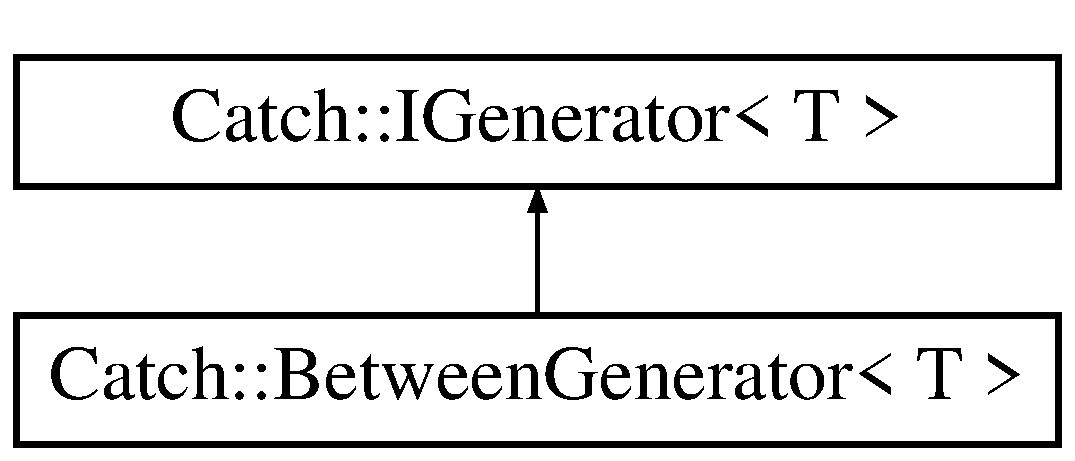
\includegraphics[height=2.000000cm]{classCatch_1_1BetweenGenerator}
\end{center}
\end{figure}
\subsection*{Public Member Functions}
\begin{DoxyCompactItemize}
\item 
\hyperlink{classCatch_1_1BetweenGenerator_a835a057d691ae37caef660624099b51c}{Between\-Generator} (T from, T to)
\item 
virtual T \hyperlink{classCatch_1_1BetweenGenerator_af83575d62cc727ca995446cff4d6c26c}{get\-Value} (std\-::size\-\_\-t index) const 
\item 
virtual std\-::size\-\_\-t \hyperlink{classCatch_1_1BetweenGenerator_aa53a04a259e796ba2b5adabed79474b5}{size} () const 
\end{DoxyCompactItemize}


\subsection{Constructor \& Destructor Documentation}
\hypertarget{classCatch_1_1BetweenGenerator_a835a057d691ae37caef660624099b51c}{\index{Catch\-::\-Between\-Generator@{Catch\-::\-Between\-Generator}!Between\-Generator@{Between\-Generator}}
\index{Between\-Generator@{Between\-Generator}!Catch::BetweenGenerator@{Catch\-::\-Between\-Generator}}
\subsubsection[{Between\-Generator}]{\setlength{\rightskip}{0pt plus 5cm}template$<$typename T $>$ {\bf Catch\-::\-Between\-Generator}$<$ T $>$\-::{\bf Between\-Generator} (
\begin{DoxyParamCaption}
\item[{T}]{from, }
\item[{T}]{to}
\end{DoxyParamCaption}
)\hspace{0.3cm}{\ttfamily [inline]}}}\label{classCatch_1_1BetweenGenerator_a835a057d691ae37caef660624099b51c}


\subsection{Member Function Documentation}
\hypertarget{classCatch_1_1BetweenGenerator_af83575d62cc727ca995446cff4d6c26c}{\index{Catch\-::\-Between\-Generator@{Catch\-::\-Between\-Generator}!get\-Value@{get\-Value}}
\index{get\-Value@{get\-Value}!Catch::BetweenGenerator@{Catch\-::\-Between\-Generator}}
\subsubsection[{get\-Value}]{\setlength{\rightskip}{0pt plus 5cm}template$<$typename T $>$ virtual T {\bf Catch\-::\-Between\-Generator}$<$ T $>$\-::get\-Value (
\begin{DoxyParamCaption}
\item[{std\-::size\-\_\-t}]{index}
\end{DoxyParamCaption}
) const\hspace{0.3cm}{\ttfamily [inline]}, {\ttfamily [virtual]}}}\label{classCatch_1_1BetweenGenerator_af83575d62cc727ca995446cff4d6c26c}


Implements \hyperlink{structCatch_1_1IGenerator_ad69e937cb66dba3ed9429c42abf4fce3}{Catch\-::\-I\-Generator$<$ T $>$}.

\hypertarget{classCatch_1_1BetweenGenerator_aa53a04a259e796ba2b5adabed79474b5}{\index{Catch\-::\-Between\-Generator@{Catch\-::\-Between\-Generator}!size@{size}}
\index{size@{size}!Catch::BetweenGenerator@{Catch\-::\-Between\-Generator}}
\subsubsection[{size}]{\setlength{\rightskip}{0pt plus 5cm}template$<$typename T $>$ virtual std\-::size\-\_\-t {\bf Catch\-::\-Between\-Generator}$<$ T $>$\-::size (
\begin{DoxyParamCaption}
{}
\end{DoxyParamCaption}
) const\hspace{0.3cm}{\ttfamily [inline]}, {\ttfamily [virtual]}}}\label{classCatch_1_1BetweenGenerator_aa53a04a259e796ba2b5adabed79474b5}


Implements \hyperlink{structCatch_1_1IGenerator_a2e317253b03e838b6065ce69719a198e}{Catch\-::\-I\-Generator$<$ T $>$}.



The documentation for this class was generated from the following file\-:\begin{DoxyCompactItemize}
\item 
/home/alexander/\-Un\-B/\-M\-P/\-Trabalho\-\_\-2\-\_\-\-M\-P\-\_\-\-Alexander\-\_\-13\-\_\-0039853/include/\hyperlink{catch_8hpp}{catch.\-hpp}\end{DoxyCompactItemize}

\hypertarget{classCatch_1_1BinaryExpression}{\section{Catch\-:\-:Binary\-Expression$<$ Lhs\-T, Op, Rhs\-T $>$ Class Template Reference}
\label{classCatch_1_1BinaryExpression}\index{Catch\-::\-Binary\-Expression$<$ Lhs\-T, Op, Rhs\-T $>$@{Catch\-::\-Binary\-Expression$<$ Lhs\-T, Op, Rhs\-T $>$}}
}


{\ttfamily \#include $<$catch.\-hpp$>$}

Inheritance diagram for Catch\-:\-:Binary\-Expression$<$ Lhs\-T, Op, Rhs\-T $>$\-:\begin{figure}[H]
\begin{center}
\leavevmode
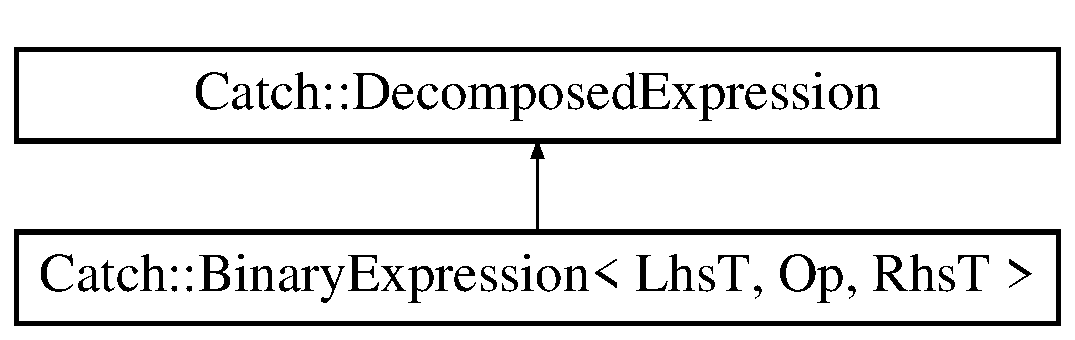
\includegraphics[height=2.000000cm]{classCatch_1_1BinaryExpression}
\end{center}
\end{figure}
\subsection*{Public Member Functions}
\begin{DoxyCompactItemize}
\item 
\hyperlink{classCatch_1_1BinaryExpression_a0d81384761aba5f7a6d5f4fc7e7944f3}{Binary\-Expression} (\hyperlink{classCatch_1_1ResultBuilder}{Result\-Builder} \&rb, Lhs\-T lhs, Rhs\-T rhs)
\item 
\hyperlink{classCatch_1_1BinaryExpression}{Binary\-Expression} \& \hyperlink{classCatch_1_1BinaryExpression_a2147a858eb5866e5643d0ef321064aa1}{operator=} (\hyperlink{classCatch_1_1BinaryExpression}{Binary\-Expression} \&)
\item 
void \hyperlink{classCatch_1_1BinaryExpression_a480b1d75bbac51d1936aec7dad8c1cb1}{end\-Expression} () const 
\item 
virtual bool \hyperlink{classCatch_1_1BinaryExpression_a4c617c0b6a73a9cafbbf900909c7c258}{is\-Binary\-Expression} () const \hyperlink{catch_8hpp_a8ecdce4d3f57835f707915ae831eb847}{C\-A\-T\-C\-H\-\_\-\-O\-V\-E\-R\-R\-I\-D\-E}
\item 
virtual void \hyperlink{classCatch_1_1BinaryExpression_a6ed73ff9af9c229f9fa3d35d019f9e37}{reconstruct\-Expression} (std\-::string \&dest) const \hyperlink{catch_8hpp_a8ecdce4d3f57835f707915ae831eb847}{C\-A\-T\-C\-H\-\_\-\-O\-V\-E\-R\-R\-I\-D\-E}
\end{DoxyCompactItemize}


\subsection{Constructor \& Destructor Documentation}
\hypertarget{classCatch_1_1BinaryExpression_a0d81384761aba5f7a6d5f4fc7e7944f3}{\index{Catch\-::\-Binary\-Expression@{Catch\-::\-Binary\-Expression}!Binary\-Expression@{Binary\-Expression}}
\index{Binary\-Expression@{Binary\-Expression}!Catch::BinaryExpression@{Catch\-::\-Binary\-Expression}}
\subsubsection[{Binary\-Expression}]{\setlength{\rightskip}{0pt plus 5cm}template$<$typename Lhs\-T, Internal\-::\-Operator Op, typename Rhs\-T$>$ {\bf Catch\-::\-Binary\-Expression}$<$ Lhs\-T, Op, Rhs\-T $>$\-::{\bf Binary\-Expression} (
\begin{DoxyParamCaption}
\item[{{\bf Result\-Builder} \&}]{rb, }
\item[{Lhs\-T}]{lhs, }
\item[{Rhs\-T}]{rhs}
\end{DoxyParamCaption}
)\hspace{0.3cm}{\ttfamily [inline]}}}\label{classCatch_1_1BinaryExpression_a0d81384761aba5f7a6d5f4fc7e7944f3}


\subsection{Member Function Documentation}
\hypertarget{classCatch_1_1BinaryExpression_a480b1d75bbac51d1936aec7dad8c1cb1}{\index{Catch\-::\-Binary\-Expression@{Catch\-::\-Binary\-Expression}!end\-Expression@{end\-Expression}}
\index{end\-Expression@{end\-Expression}!Catch::BinaryExpression@{Catch\-::\-Binary\-Expression}}
\subsubsection[{end\-Expression}]{\setlength{\rightskip}{0pt plus 5cm}template$<$typename Lhs\-T, Internal\-::\-Operator Op, typename Rhs\-T$>$ void {\bf Catch\-::\-Binary\-Expression}$<$ Lhs\-T, Op, Rhs\-T $>$\-::end\-Expression (
\begin{DoxyParamCaption}
{}
\end{DoxyParamCaption}
) const\hspace{0.3cm}{\ttfamily [inline]}}}\label{classCatch_1_1BinaryExpression_a480b1d75bbac51d1936aec7dad8c1cb1}
\hypertarget{classCatch_1_1BinaryExpression_a4c617c0b6a73a9cafbbf900909c7c258}{\index{Catch\-::\-Binary\-Expression@{Catch\-::\-Binary\-Expression}!is\-Binary\-Expression@{is\-Binary\-Expression}}
\index{is\-Binary\-Expression@{is\-Binary\-Expression}!Catch::BinaryExpression@{Catch\-::\-Binary\-Expression}}
\subsubsection[{is\-Binary\-Expression}]{\setlength{\rightskip}{0pt plus 5cm}template$<$typename Lhs\-T, Internal\-::\-Operator Op, typename Rhs\-T$>$ virtual bool {\bf Catch\-::\-Binary\-Expression}$<$ Lhs\-T, Op, Rhs\-T $>$\-::is\-Binary\-Expression (
\begin{DoxyParamCaption}
{}
\end{DoxyParamCaption}
) const\hspace{0.3cm}{\ttfamily [inline]}, {\ttfamily [virtual]}}}\label{classCatch_1_1BinaryExpression_a4c617c0b6a73a9cafbbf900909c7c258}


Reimplemented from \hyperlink{structCatch_1_1DecomposedExpression_af08ea5b188f04b0f441d8e4cdc340452}{Catch\-::\-Decomposed\-Expression}.

\hypertarget{classCatch_1_1BinaryExpression_a2147a858eb5866e5643d0ef321064aa1}{\index{Catch\-::\-Binary\-Expression@{Catch\-::\-Binary\-Expression}!operator=@{operator=}}
\index{operator=@{operator=}!Catch::BinaryExpression@{Catch\-::\-Binary\-Expression}}
\subsubsection[{operator=}]{\setlength{\rightskip}{0pt plus 5cm}template$<$typename Lhs\-T, Internal\-::\-Operator Op, typename Rhs\-T$>$ {\bf Binary\-Expression}\& {\bf Catch\-::\-Binary\-Expression}$<$ Lhs\-T, Op, Rhs\-T $>$\-::operator= (
\begin{DoxyParamCaption}
\item[{{\bf Binary\-Expression}$<$ Lhs\-T, Op, Rhs\-T $>$ \&}]{}
\end{DoxyParamCaption}
)}}\label{classCatch_1_1BinaryExpression_a2147a858eb5866e5643d0ef321064aa1}
\hypertarget{classCatch_1_1BinaryExpression_a6ed73ff9af9c229f9fa3d35d019f9e37}{\index{Catch\-::\-Binary\-Expression@{Catch\-::\-Binary\-Expression}!reconstruct\-Expression@{reconstruct\-Expression}}
\index{reconstruct\-Expression@{reconstruct\-Expression}!Catch::BinaryExpression@{Catch\-::\-Binary\-Expression}}
\subsubsection[{reconstruct\-Expression}]{\setlength{\rightskip}{0pt plus 5cm}template$<$typename Lhs\-T, Internal\-::\-Operator Op, typename Rhs\-T$>$ virtual void {\bf Catch\-::\-Binary\-Expression}$<$ Lhs\-T, Op, Rhs\-T $>$\-::reconstruct\-Expression (
\begin{DoxyParamCaption}
\item[{std\-::string \&}]{dest}
\end{DoxyParamCaption}
) const\hspace{0.3cm}{\ttfamily [inline]}, {\ttfamily [virtual]}}}\label{classCatch_1_1BinaryExpression_a6ed73ff9af9c229f9fa3d35d019f9e37}


Implements \hyperlink{structCatch_1_1DecomposedExpression_a9ce7f356dc96f11f80e40c82f5aa7e55}{Catch\-::\-Decomposed\-Expression}.



The documentation for this class was generated from the following file\-:\begin{DoxyCompactItemize}
\item 
/home/alexander/\-Un\-B/\-M\-P/\-Trabalho\-\_\-2\-\_\-\-M\-P\-\_\-\-Alexander\-\_\-13\-\_\-0039853/include/\hyperlink{catch_8hpp}{catch.\-hpp}\end{DoxyCompactItemize}

\hypertarget{structCatch_1_1Detail_1_1BorgType}{\section{Catch\-:\-:Detail\-:\-:Borg\-Type Struct Reference}
\label{structCatch_1_1Detail_1_1BorgType}\index{Catch\-::\-Detail\-::\-Borg\-Type@{Catch\-::\-Detail\-::\-Borg\-Type}}
}


{\ttfamily \#include $<$catch.\-hpp$>$}

\subsection*{Public Member Functions}
\begin{DoxyCompactItemize}
\item 
{\footnotesize template$<$typename T $>$ }\\\hyperlink{structCatch_1_1Detail_1_1BorgType_a780a9946ed0d654f0bfc043c8fc505d8}{Borg\-Type} (T const \&)
\end{DoxyCompactItemize}


\subsection{Constructor \& Destructor Documentation}
\hypertarget{structCatch_1_1Detail_1_1BorgType_a780a9946ed0d654f0bfc043c8fc505d8}{\index{Catch\-::\-Detail\-::\-Borg\-Type@{Catch\-::\-Detail\-::\-Borg\-Type}!Borg\-Type@{Borg\-Type}}
\index{Borg\-Type@{Borg\-Type}!Catch::Detail::BorgType@{Catch\-::\-Detail\-::\-Borg\-Type}}
\subsubsection[{Borg\-Type}]{\setlength{\rightskip}{0pt plus 5cm}template$<$typename T $>$ Catch\-::\-Detail\-::\-Borg\-Type\-::\-Borg\-Type (
\begin{DoxyParamCaption}
\item[{T const \&}]{}
\end{DoxyParamCaption}
)}}\label{structCatch_1_1Detail_1_1BorgType_a780a9946ed0d654f0bfc043c8fc505d8}


The documentation for this struct was generated from the following file\-:\begin{DoxyCompactItemize}
\item 
/home/alexander/\-Un\-B/\-M\-P/\-Trabalho\-\_\-2\-\_\-\-M\-P\-\_\-\-Alexander\-\_\-13\-\_\-0039853/include/\hyperlink{catch_8hpp}{catch.\-hpp}\end{DoxyCompactItemize}

\hypertarget{structCatch_1_1Matchers_1_1StdString_1_1CasedString}{\section{Catch\-:\-:Matchers\-:\-:Std\-String\-:\-:Cased\-String Struct Reference}
\label{structCatch_1_1Matchers_1_1StdString_1_1CasedString}\index{Catch\-::\-Matchers\-::\-Std\-String\-::\-Cased\-String@{Catch\-::\-Matchers\-::\-Std\-String\-::\-Cased\-String}}
}


{\ttfamily \#include $<$catch.\-hpp$>$}

\subsection*{Public Member Functions}
\begin{DoxyCompactItemize}
\item 
\hyperlink{structCatch_1_1Matchers_1_1StdString_1_1CasedString_aa88bbc5acd2bff22351d8d4b1816b561}{Cased\-String} (std\-::string const \&str, \hyperlink{structCatch_1_1CaseSensitive_aad49d3aee2d97066642fffa919685c6a}{Case\-Sensitive\-::\-Choice} case\-Sensitivity)
\item 
std\-::string \hyperlink{structCatch_1_1Matchers_1_1StdString_1_1CasedString_a0ff84e194426c8f4bca0660b9180d20d}{adjust\-String} (std\-::string const \&str) const 
\item 
std\-::string \hyperlink{structCatch_1_1Matchers_1_1StdString_1_1CasedString_a1113c80dd02967032a99290bdcd1b590}{case\-Sensitivity\-Suffix} () const 
\end{DoxyCompactItemize}
\subsection*{Public Attributes}
\begin{DoxyCompactItemize}
\item 
\hyperlink{structCatch_1_1CaseSensitive_aad49d3aee2d97066642fffa919685c6a}{Case\-Sensitive\-::\-Choice} \hyperlink{structCatch_1_1Matchers_1_1StdString_1_1CasedString_ae1c2864c986941536a6e94cca0528f92}{m\-\_\-case\-Sensitivity}
\item 
std\-::string \hyperlink{structCatch_1_1Matchers_1_1StdString_1_1CasedString_ad05dbc99aba3c3c386d6b856b213f911}{m\-\_\-str}
\end{DoxyCompactItemize}


\subsection{Constructor \& Destructor Documentation}
\hypertarget{structCatch_1_1Matchers_1_1StdString_1_1CasedString_aa88bbc5acd2bff22351d8d4b1816b561}{\index{Catch\-::\-Matchers\-::\-Std\-String\-::\-Cased\-String@{Catch\-::\-Matchers\-::\-Std\-String\-::\-Cased\-String}!Cased\-String@{Cased\-String}}
\index{Cased\-String@{Cased\-String}!Catch::Matchers::StdString::CasedString@{Catch\-::\-Matchers\-::\-Std\-String\-::\-Cased\-String}}
\subsubsection[{Cased\-String}]{\setlength{\rightskip}{0pt plus 5cm}Catch\-::\-Matchers\-::\-Std\-String\-::\-Cased\-String\-::\-Cased\-String (
\begin{DoxyParamCaption}
\item[{std\-::string const \&}]{str, }
\item[{{\bf Case\-Sensitive\-::\-Choice}}]{case\-Sensitivity}
\end{DoxyParamCaption}
)}}\label{structCatch_1_1Matchers_1_1StdString_1_1CasedString_aa88bbc5acd2bff22351d8d4b1816b561}


\subsection{Member Function Documentation}
\hypertarget{structCatch_1_1Matchers_1_1StdString_1_1CasedString_a0ff84e194426c8f4bca0660b9180d20d}{\index{Catch\-::\-Matchers\-::\-Std\-String\-::\-Cased\-String@{Catch\-::\-Matchers\-::\-Std\-String\-::\-Cased\-String}!adjust\-String@{adjust\-String}}
\index{adjust\-String@{adjust\-String}!Catch::Matchers::StdString::CasedString@{Catch\-::\-Matchers\-::\-Std\-String\-::\-Cased\-String}}
\subsubsection[{adjust\-String}]{\setlength{\rightskip}{0pt plus 5cm}std\-::string Catch\-::\-Matchers\-::\-Std\-String\-::\-Cased\-String\-::adjust\-String (
\begin{DoxyParamCaption}
\item[{std\-::string const \&}]{str}
\end{DoxyParamCaption}
) const}}\label{structCatch_1_1Matchers_1_1StdString_1_1CasedString_a0ff84e194426c8f4bca0660b9180d20d}
\hypertarget{structCatch_1_1Matchers_1_1StdString_1_1CasedString_a1113c80dd02967032a99290bdcd1b590}{\index{Catch\-::\-Matchers\-::\-Std\-String\-::\-Cased\-String@{Catch\-::\-Matchers\-::\-Std\-String\-::\-Cased\-String}!case\-Sensitivity\-Suffix@{case\-Sensitivity\-Suffix}}
\index{case\-Sensitivity\-Suffix@{case\-Sensitivity\-Suffix}!Catch::Matchers::StdString::CasedString@{Catch\-::\-Matchers\-::\-Std\-String\-::\-Cased\-String}}
\subsubsection[{case\-Sensitivity\-Suffix}]{\setlength{\rightskip}{0pt plus 5cm}std\-::string Catch\-::\-Matchers\-::\-Std\-String\-::\-Cased\-String\-::case\-Sensitivity\-Suffix (
\begin{DoxyParamCaption}
{}
\end{DoxyParamCaption}
) const}}\label{structCatch_1_1Matchers_1_1StdString_1_1CasedString_a1113c80dd02967032a99290bdcd1b590}


\subsection{Member Data Documentation}
\hypertarget{structCatch_1_1Matchers_1_1StdString_1_1CasedString_ae1c2864c986941536a6e94cca0528f92}{\index{Catch\-::\-Matchers\-::\-Std\-String\-::\-Cased\-String@{Catch\-::\-Matchers\-::\-Std\-String\-::\-Cased\-String}!m\-\_\-case\-Sensitivity@{m\-\_\-case\-Sensitivity}}
\index{m\-\_\-case\-Sensitivity@{m\-\_\-case\-Sensitivity}!Catch::Matchers::StdString::CasedString@{Catch\-::\-Matchers\-::\-Std\-String\-::\-Cased\-String}}
\subsubsection[{m\-\_\-case\-Sensitivity}]{\setlength{\rightskip}{0pt plus 5cm}{\bf Case\-Sensitive\-::\-Choice} Catch\-::\-Matchers\-::\-Std\-String\-::\-Cased\-String\-::m\-\_\-case\-Sensitivity}}\label{structCatch_1_1Matchers_1_1StdString_1_1CasedString_ae1c2864c986941536a6e94cca0528f92}
\hypertarget{structCatch_1_1Matchers_1_1StdString_1_1CasedString_ad05dbc99aba3c3c386d6b856b213f911}{\index{Catch\-::\-Matchers\-::\-Std\-String\-::\-Cased\-String@{Catch\-::\-Matchers\-::\-Std\-String\-::\-Cased\-String}!m\-\_\-str@{m\-\_\-str}}
\index{m\-\_\-str@{m\-\_\-str}!Catch::Matchers::StdString::CasedString@{Catch\-::\-Matchers\-::\-Std\-String\-::\-Cased\-String}}
\subsubsection[{m\-\_\-str}]{\setlength{\rightskip}{0pt plus 5cm}std\-::string Catch\-::\-Matchers\-::\-Std\-String\-::\-Cased\-String\-::m\-\_\-str}}\label{structCatch_1_1Matchers_1_1StdString_1_1CasedString_ad05dbc99aba3c3c386d6b856b213f911}


The documentation for this struct was generated from the following file\-:\begin{DoxyCompactItemize}
\item 
/home/alexander/\-Un\-B/\-M\-P/\-Trabalho\-\_\-2\-\_\-\-M\-P\-\_\-\-Alexander\-\_\-13\-\_\-0039853/include/\hyperlink{catch_8hpp}{catch.\-hpp}\end{DoxyCompactItemize}

\hypertarget{structCatch_1_1CaseSensitive}{\section{Catch\-:\-:Case\-Sensitive Struct Reference}
\label{structCatch_1_1CaseSensitive}\index{Catch\-::\-Case\-Sensitive@{Catch\-::\-Case\-Sensitive}}
}


{\ttfamily \#include $<$catch.\-hpp$>$}

\subsection*{Public Types}
\begin{DoxyCompactItemize}
\item 
enum \hyperlink{structCatch_1_1CaseSensitive_aad49d3aee2d97066642fffa919685c6a}{Choice} \{ \hyperlink{structCatch_1_1CaseSensitive_aad49d3aee2d97066642fffa919685c6aa7c5550b69ec3c502e6f609b67f9613c6}{Yes}, 
\hyperlink{structCatch_1_1CaseSensitive_aad49d3aee2d97066642fffa919685c6aa4ffff8d29b481f0116abc37228cd53f6}{No}
 \}
\end{DoxyCompactItemize}


\subsection{Member Enumeration Documentation}
\hypertarget{structCatch_1_1CaseSensitive_aad49d3aee2d97066642fffa919685c6a}{\index{Catch\-::\-Case\-Sensitive@{Catch\-::\-Case\-Sensitive}!Choice@{Choice}}
\index{Choice@{Choice}!Catch::CaseSensitive@{Catch\-::\-Case\-Sensitive}}
\subsubsection[{Choice}]{\setlength{\rightskip}{0pt plus 5cm}enum {\bf Catch\-::\-Case\-Sensitive\-::\-Choice}}}\label{structCatch_1_1CaseSensitive_aad49d3aee2d97066642fffa919685c6a}
\begin{Desc}
\item[Enumerator]\par
\begin{description}
\index{Yes@{Yes}!Catch\-::\-Case\-Sensitive@{Catch\-::\-Case\-Sensitive}}\index{Catch\-::\-Case\-Sensitive@{Catch\-::\-Case\-Sensitive}!Yes@{Yes}}\item[{\em 
\hypertarget{structCatch_1_1CaseSensitive_aad49d3aee2d97066642fffa919685c6aa7c5550b69ec3c502e6f609b67f9613c6}{Yes}\label{structCatch_1_1CaseSensitive_aad49d3aee2d97066642fffa919685c6aa7c5550b69ec3c502e6f609b67f9613c6}
}]\index{No@{No}!Catch\-::\-Case\-Sensitive@{Catch\-::\-Case\-Sensitive}}\index{Catch\-::\-Case\-Sensitive@{Catch\-::\-Case\-Sensitive}!No@{No}}\item[{\em 
\hypertarget{structCatch_1_1CaseSensitive_aad49d3aee2d97066642fffa919685c6aa4ffff8d29b481f0116abc37228cd53f6}{No}\label{structCatch_1_1CaseSensitive_aad49d3aee2d97066642fffa919685c6aa4ffff8d29b481f0116abc37228cd53f6}
}]\end{description}
\end{Desc}


The documentation for this struct was generated from the following file\-:\begin{DoxyCompactItemize}
\item 
/home/alexander/\-Un\-B/\-M\-P/\-Trabalho\-\_\-2\-\_\-\-M\-P\-\_\-\-Alexander\-\_\-13\-\_\-0039853/include/\hyperlink{catch_8hpp}{catch.\-hpp}\end{DoxyCompactItemize}

\hypertarget{classCatch_1_1CompositeGenerator}{\section{Catch\-:\-:Composite\-Generator$<$ T $>$ Class Template Reference}
\label{classCatch_1_1CompositeGenerator}\index{Catch\-::\-Composite\-Generator$<$ T $>$@{Catch\-::\-Composite\-Generator$<$ T $>$}}
}


{\ttfamily \#include $<$catch.\-hpp$>$}

\subsection*{Public Member Functions}
\begin{DoxyCompactItemize}
\item 
\hyperlink{classCatch_1_1CompositeGenerator_a923398b140371d1783858766864a1af5}{Composite\-Generator} ()
\item 
\hyperlink{classCatch_1_1CompositeGenerator_a21a7070a00e4a6fe021294c356692692}{Composite\-Generator} (\hyperlink{classCatch_1_1CompositeGenerator}{Composite\-Generator} \&other)
\item 
\hyperlink{classCatch_1_1CompositeGenerator}{Composite\-Generator} \& \hyperlink{classCatch_1_1CompositeGenerator_ac3c57cf4ca5472f440bf71e2936bcd4a}{set\-File\-Info} (const char $\ast$file\-Info)
\item 
\hyperlink{classCatch_1_1CompositeGenerator_a5766205abd7004c508c20ddbb5e5555e}{$\sim$\-Composite\-Generator} ()
\item 
\hyperlink{classCatch_1_1CompositeGenerator_aa3f627d84fb256df0404d19d7fd4b784}{operator T} () const 
\item 
void \hyperlink{classCatch_1_1CompositeGenerator_af3774d42ad2d3453d089ca599efe0517}{add} (const \hyperlink{structCatch_1_1IGenerator}{I\-Generator}$<$ T $>$ $\ast$generator)
\item 
\hyperlink{classCatch_1_1CompositeGenerator}{Composite\-Generator} \& \hyperlink{classCatch_1_1CompositeGenerator_a2e03f42df85cdd238aabd77a80b075d5}{then} (\hyperlink{classCatch_1_1CompositeGenerator}{Composite\-Generator} \&other)
\item 
\hyperlink{classCatch_1_1CompositeGenerator}{Composite\-Generator} \& \hyperlink{classCatch_1_1CompositeGenerator_aefdc11bcfccdf07d2db5f0da3ed8758c}{then} (T value)
\end{DoxyCompactItemize}


\subsection{Constructor \& Destructor Documentation}
\hypertarget{classCatch_1_1CompositeGenerator_a923398b140371d1783858766864a1af5}{\index{Catch\-::\-Composite\-Generator@{Catch\-::\-Composite\-Generator}!Composite\-Generator@{Composite\-Generator}}
\index{Composite\-Generator@{Composite\-Generator}!Catch::CompositeGenerator@{Catch\-::\-Composite\-Generator}}
\subsubsection[{Composite\-Generator}]{\setlength{\rightskip}{0pt plus 5cm}template$<$typename T$>$ {\bf Catch\-::\-Composite\-Generator}$<$ T $>$\-::{\bf Composite\-Generator} (
\begin{DoxyParamCaption}
{}
\end{DoxyParamCaption}
)\hspace{0.3cm}{\ttfamily [inline]}}}\label{classCatch_1_1CompositeGenerator_a923398b140371d1783858766864a1af5}
\hypertarget{classCatch_1_1CompositeGenerator_a21a7070a00e4a6fe021294c356692692}{\index{Catch\-::\-Composite\-Generator@{Catch\-::\-Composite\-Generator}!Composite\-Generator@{Composite\-Generator}}
\index{Composite\-Generator@{Composite\-Generator}!Catch::CompositeGenerator@{Catch\-::\-Composite\-Generator}}
\subsubsection[{Composite\-Generator}]{\setlength{\rightskip}{0pt plus 5cm}template$<$typename T$>$ {\bf Catch\-::\-Composite\-Generator}$<$ T $>$\-::{\bf Composite\-Generator} (
\begin{DoxyParamCaption}
\item[{{\bf Composite\-Generator}$<$ T $>$ \&}]{other}
\end{DoxyParamCaption}
)\hspace{0.3cm}{\ttfamily [inline]}}}\label{classCatch_1_1CompositeGenerator_a21a7070a00e4a6fe021294c356692692}
\hypertarget{classCatch_1_1CompositeGenerator_a5766205abd7004c508c20ddbb5e5555e}{\index{Catch\-::\-Composite\-Generator@{Catch\-::\-Composite\-Generator}!$\sim$\-Composite\-Generator@{$\sim$\-Composite\-Generator}}
\index{$\sim$\-Composite\-Generator@{$\sim$\-Composite\-Generator}!Catch::CompositeGenerator@{Catch\-::\-Composite\-Generator}}
\subsubsection[{$\sim$\-Composite\-Generator}]{\setlength{\rightskip}{0pt plus 5cm}template$<$typename T$>$ {\bf Catch\-::\-Composite\-Generator}$<$ T $>$\-::$\sim${\bf Composite\-Generator} (
\begin{DoxyParamCaption}
{}
\end{DoxyParamCaption}
)\hspace{0.3cm}{\ttfamily [inline]}}}\label{classCatch_1_1CompositeGenerator_a5766205abd7004c508c20ddbb5e5555e}


\subsection{Member Function Documentation}
\hypertarget{classCatch_1_1CompositeGenerator_af3774d42ad2d3453d089ca599efe0517}{\index{Catch\-::\-Composite\-Generator@{Catch\-::\-Composite\-Generator}!add@{add}}
\index{add@{add}!Catch::CompositeGenerator@{Catch\-::\-Composite\-Generator}}
\subsubsection[{add}]{\setlength{\rightskip}{0pt plus 5cm}template$<$typename T$>$ void {\bf Catch\-::\-Composite\-Generator}$<$ T $>$\-::add (
\begin{DoxyParamCaption}
\item[{const {\bf I\-Generator}$<$ T $>$ $\ast$}]{generator}
\end{DoxyParamCaption}
)\hspace{0.3cm}{\ttfamily [inline]}}}\label{classCatch_1_1CompositeGenerator_af3774d42ad2d3453d089ca599efe0517}
\hypertarget{classCatch_1_1CompositeGenerator_aa3f627d84fb256df0404d19d7fd4b784}{\index{Catch\-::\-Composite\-Generator@{Catch\-::\-Composite\-Generator}!operator T@{operator T}}
\index{operator T@{operator T}!Catch::CompositeGenerator@{Catch\-::\-Composite\-Generator}}
\subsubsection[{operator T}]{\setlength{\rightskip}{0pt plus 5cm}template$<$typename T$>$ {\bf Catch\-::\-Composite\-Generator}$<$ T $>$\-::operator T (
\begin{DoxyParamCaption}
{}
\end{DoxyParamCaption}
) const\hspace{0.3cm}{\ttfamily [inline]}}}\label{classCatch_1_1CompositeGenerator_aa3f627d84fb256df0404d19d7fd4b784}
\hypertarget{classCatch_1_1CompositeGenerator_ac3c57cf4ca5472f440bf71e2936bcd4a}{\index{Catch\-::\-Composite\-Generator@{Catch\-::\-Composite\-Generator}!set\-File\-Info@{set\-File\-Info}}
\index{set\-File\-Info@{set\-File\-Info}!Catch::CompositeGenerator@{Catch\-::\-Composite\-Generator}}
\subsubsection[{set\-File\-Info}]{\setlength{\rightskip}{0pt plus 5cm}template$<$typename T$>$ {\bf Composite\-Generator}\& {\bf Catch\-::\-Composite\-Generator}$<$ T $>$\-::set\-File\-Info (
\begin{DoxyParamCaption}
\item[{const char $\ast$}]{file\-Info}
\end{DoxyParamCaption}
)\hspace{0.3cm}{\ttfamily [inline]}}}\label{classCatch_1_1CompositeGenerator_ac3c57cf4ca5472f440bf71e2936bcd4a}
\hypertarget{classCatch_1_1CompositeGenerator_a2e03f42df85cdd238aabd77a80b075d5}{\index{Catch\-::\-Composite\-Generator@{Catch\-::\-Composite\-Generator}!then@{then}}
\index{then@{then}!Catch::CompositeGenerator@{Catch\-::\-Composite\-Generator}}
\subsubsection[{then}]{\setlength{\rightskip}{0pt plus 5cm}template$<$typename T$>$ {\bf Composite\-Generator}\& {\bf Catch\-::\-Composite\-Generator}$<$ T $>$\-::then (
\begin{DoxyParamCaption}
\item[{{\bf Composite\-Generator}$<$ T $>$ \&}]{other}
\end{DoxyParamCaption}
)\hspace{0.3cm}{\ttfamily [inline]}}}\label{classCatch_1_1CompositeGenerator_a2e03f42df85cdd238aabd77a80b075d5}
\hypertarget{classCatch_1_1CompositeGenerator_aefdc11bcfccdf07d2db5f0da3ed8758c}{\index{Catch\-::\-Composite\-Generator@{Catch\-::\-Composite\-Generator}!then@{then}}
\index{then@{then}!Catch::CompositeGenerator@{Catch\-::\-Composite\-Generator}}
\subsubsection[{then}]{\setlength{\rightskip}{0pt plus 5cm}template$<$typename T$>$ {\bf Composite\-Generator}\& {\bf Catch\-::\-Composite\-Generator}$<$ T $>$\-::then (
\begin{DoxyParamCaption}
\item[{T}]{value}
\end{DoxyParamCaption}
)\hspace{0.3cm}{\ttfamily [inline]}}}\label{classCatch_1_1CompositeGenerator_aefdc11bcfccdf07d2db5f0da3ed8758c}


The documentation for this class was generated from the following file\-:\begin{DoxyCompactItemize}
\item 
/home/alexander/\-Un\-B/\-M\-P/\-Trabalho\-\_\-2\-\_\-\-M\-P\-\_\-\-Alexander\-\_\-13\-\_\-0039853/include/\hyperlink{catch_8hpp}{catch.\-hpp}\end{DoxyCompactItemize}

\hypertarget{structCatch_1_1Matchers_1_1Vector_1_1ContainsElementMatcher}{\section{Catch\-:\-:Matchers\-:\-:Vector\-:\-:Contains\-Element\-Matcher$<$ T $>$ Struct Template Reference}
\label{structCatch_1_1Matchers_1_1Vector_1_1ContainsElementMatcher}\index{Catch\-::\-Matchers\-::\-Vector\-::\-Contains\-Element\-Matcher$<$ T $>$@{Catch\-::\-Matchers\-::\-Vector\-::\-Contains\-Element\-Matcher$<$ T $>$}}
}


{\ttfamily \#include $<$catch.\-hpp$>$}

Inheritance diagram for Catch\-:\-:Matchers\-:\-:Vector\-:\-:Contains\-Element\-Matcher$<$ T $>$\-:\begin{figure}[H]
\begin{center}
\leavevmode
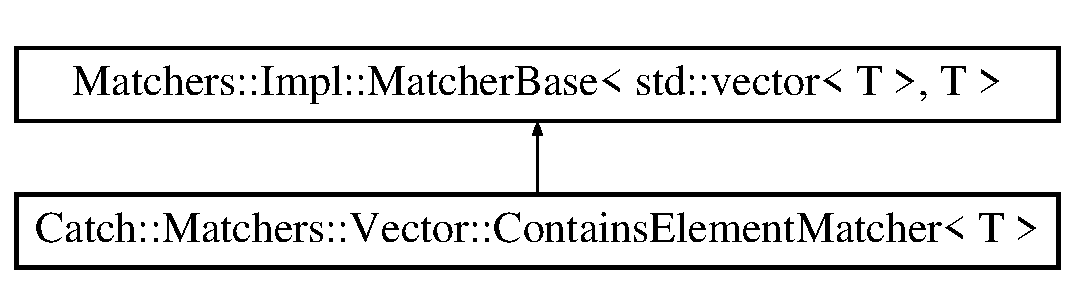
\includegraphics[height=2.000000cm]{structCatch_1_1Matchers_1_1Vector_1_1ContainsElementMatcher}
\end{center}
\end{figure}
\subsection*{Public Member Functions}
\begin{DoxyCompactItemize}
\item 
\hyperlink{structCatch_1_1Matchers_1_1Vector_1_1ContainsElementMatcher_a6a05740b5d3f89fac8de84ac0cff7b93}{Contains\-Element\-Matcher} (T const \&comparator)
\item 
bool \hyperlink{structCatch_1_1Matchers_1_1Vector_1_1ContainsElementMatcher_a95fd99879bcfbe129898bef922c92c17}{match} (std\-::vector$<$ T $>$ const \&v) const \hyperlink{catch_8hpp_a8ecdce4d3f57835f707915ae831eb847}{C\-A\-T\-C\-H\-\_\-\-O\-V\-E\-R\-R\-I\-D\-E}
\item 
virtual std\-::string \hyperlink{structCatch_1_1Matchers_1_1Vector_1_1ContainsElementMatcher_a5a869772714dd045816707b74b217664}{describe} () const \hyperlink{catch_8hpp_a8ecdce4d3f57835f707915ae831eb847}{C\-A\-T\-C\-H\-\_\-\-O\-V\-E\-R\-R\-I\-D\-E}
\end{DoxyCompactItemize}
\subsection*{Public Attributes}
\begin{DoxyCompactItemize}
\item 
T const \& \hyperlink{structCatch_1_1Matchers_1_1Vector_1_1ContainsElementMatcher_ab7eada6c4bbce1d21b44773262f9cb23}{m\-\_\-comparator}
\end{DoxyCompactItemize}


\subsection{Constructor \& Destructor Documentation}
\hypertarget{structCatch_1_1Matchers_1_1Vector_1_1ContainsElementMatcher_a6a05740b5d3f89fac8de84ac0cff7b93}{\index{Catch\-::\-Matchers\-::\-Vector\-::\-Contains\-Element\-Matcher@{Catch\-::\-Matchers\-::\-Vector\-::\-Contains\-Element\-Matcher}!Contains\-Element\-Matcher@{Contains\-Element\-Matcher}}
\index{Contains\-Element\-Matcher@{Contains\-Element\-Matcher}!Catch::Matchers::Vector::ContainsElementMatcher@{Catch\-::\-Matchers\-::\-Vector\-::\-Contains\-Element\-Matcher}}
\subsubsection[{Contains\-Element\-Matcher}]{\setlength{\rightskip}{0pt plus 5cm}template$<$typename T $>$ {\bf Catch\-::\-Matchers\-::\-Vector\-::\-Contains\-Element\-Matcher}$<$ T $>$\-::{\bf Contains\-Element\-Matcher} (
\begin{DoxyParamCaption}
\item[{T const \&}]{comparator}
\end{DoxyParamCaption}
)\hspace{0.3cm}{\ttfamily [inline]}}}\label{structCatch_1_1Matchers_1_1Vector_1_1ContainsElementMatcher_a6a05740b5d3f89fac8de84ac0cff7b93}


\subsection{Member Function Documentation}
\hypertarget{structCatch_1_1Matchers_1_1Vector_1_1ContainsElementMatcher_a5a869772714dd045816707b74b217664}{\index{Catch\-::\-Matchers\-::\-Vector\-::\-Contains\-Element\-Matcher@{Catch\-::\-Matchers\-::\-Vector\-::\-Contains\-Element\-Matcher}!describe@{describe}}
\index{describe@{describe}!Catch::Matchers::Vector::ContainsElementMatcher@{Catch\-::\-Matchers\-::\-Vector\-::\-Contains\-Element\-Matcher}}
\subsubsection[{describe}]{\setlength{\rightskip}{0pt plus 5cm}template$<$typename T $>$ virtual std\-::string {\bf Catch\-::\-Matchers\-::\-Vector\-::\-Contains\-Element\-Matcher}$<$ T $>$\-::describe (
\begin{DoxyParamCaption}
{}
\end{DoxyParamCaption}
) const\hspace{0.3cm}{\ttfamily [inline]}, {\ttfamily [virtual]}}}\label{structCatch_1_1Matchers_1_1Vector_1_1ContainsElementMatcher_a5a869772714dd045816707b74b217664}
\hypertarget{structCatch_1_1Matchers_1_1Vector_1_1ContainsElementMatcher_a95fd99879bcfbe129898bef922c92c17}{\index{Catch\-::\-Matchers\-::\-Vector\-::\-Contains\-Element\-Matcher@{Catch\-::\-Matchers\-::\-Vector\-::\-Contains\-Element\-Matcher}!match@{match}}
\index{match@{match}!Catch::Matchers::Vector::ContainsElementMatcher@{Catch\-::\-Matchers\-::\-Vector\-::\-Contains\-Element\-Matcher}}
\subsubsection[{match}]{\setlength{\rightskip}{0pt plus 5cm}template$<$typename T $>$ bool {\bf Catch\-::\-Matchers\-::\-Vector\-::\-Contains\-Element\-Matcher}$<$ T $>$\-::match (
\begin{DoxyParamCaption}
\item[{std\-::vector$<$ T $>$ const \&}]{v}
\end{DoxyParamCaption}
) const\hspace{0.3cm}{\ttfamily [inline]}}}\label{structCatch_1_1Matchers_1_1Vector_1_1ContainsElementMatcher_a95fd99879bcfbe129898bef922c92c17}


\subsection{Member Data Documentation}
\hypertarget{structCatch_1_1Matchers_1_1Vector_1_1ContainsElementMatcher_ab7eada6c4bbce1d21b44773262f9cb23}{\index{Catch\-::\-Matchers\-::\-Vector\-::\-Contains\-Element\-Matcher@{Catch\-::\-Matchers\-::\-Vector\-::\-Contains\-Element\-Matcher}!m\-\_\-comparator@{m\-\_\-comparator}}
\index{m\-\_\-comparator@{m\-\_\-comparator}!Catch::Matchers::Vector::ContainsElementMatcher@{Catch\-::\-Matchers\-::\-Vector\-::\-Contains\-Element\-Matcher}}
\subsubsection[{m\-\_\-comparator}]{\setlength{\rightskip}{0pt plus 5cm}template$<$typename T $>$ T const\& {\bf Catch\-::\-Matchers\-::\-Vector\-::\-Contains\-Element\-Matcher}$<$ T $>$\-::m\-\_\-comparator}}\label{structCatch_1_1Matchers_1_1Vector_1_1ContainsElementMatcher_ab7eada6c4bbce1d21b44773262f9cb23}


The documentation for this struct was generated from the following file\-:\begin{DoxyCompactItemize}
\item 
/home/alexander/\-Un\-B/\-M\-P/\-Trabalho\-\_\-2\-\_\-\-M\-P\-\_\-\-Alexander\-\_\-13\-\_\-0039853/include/\hyperlink{catch_8hpp}{catch.\-hpp}\end{DoxyCompactItemize}

\hypertarget{structCatch_1_1Matchers_1_1StdString_1_1ContainsMatcher}{\section{Catch\-:\-:Matchers\-:\-:Std\-String\-:\-:Contains\-Matcher Struct Reference}
\label{structCatch_1_1Matchers_1_1StdString_1_1ContainsMatcher}\index{Catch\-::\-Matchers\-::\-Std\-String\-::\-Contains\-Matcher@{Catch\-::\-Matchers\-::\-Std\-String\-::\-Contains\-Matcher}}
}


{\ttfamily \#include $<$catch.\-hpp$>$}

Inheritance diagram for Catch\-:\-:Matchers\-:\-:Std\-String\-:\-:Contains\-Matcher\-:\begin{figure}[H]
\begin{center}
\leavevmode
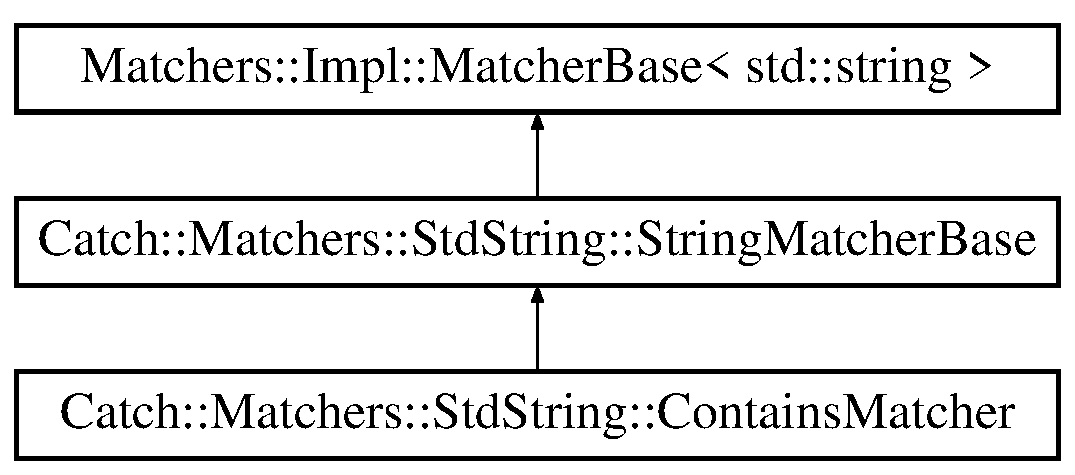
\includegraphics[height=3.000000cm]{structCatch_1_1Matchers_1_1StdString_1_1ContainsMatcher}
\end{center}
\end{figure}
\subsection*{Public Member Functions}
\begin{DoxyCompactItemize}
\item 
\hyperlink{structCatch_1_1Matchers_1_1StdString_1_1ContainsMatcher_acc892883c8409e34b28c9b39d4ef1fe3}{Contains\-Matcher} (\hyperlink{structCatch_1_1Matchers_1_1StdString_1_1CasedString}{Cased\-String} const \&comparator)
\item 
virtual bool \hyperlink{structCatch_1_1Matchers_1_1StdString_1_1ContainsMatcher_ae4d567347fa563e365f1044f29ab1042}{match} (std\-::string const \&source) const \hyperlink{catch_8hpp_a8ecdce4d3f57835f707915ae831eb847}{C\-A\-T\-C\-H\-\_\-\-O\-V\-E\-R\-R\-I\-D\-E}
\end{DoxyCompactItemize}
\subsection*{Additional Inherited Members}


\subsection{Constructor \& Destructor Documentation}
\hypertarget{structCatch_1_1Matchers_1_1StdString_1_1ContainsMatcher_acc892883c8409e34b28c9b39d4ef1fe3}{\index{Catch\-::\-Matchers\-::\-Std\-String\-::\-Contains\-Matcher@{Catch\-::\-Matchers\-::\-Std\-String\-::\-Contains\-Matcher}!Contains\-Matcher@{Contains\-Matcher}}
\index{Contains\-Matcher@{Contains\-Matcher}!Catch::Matchers::StdString::ContainsMatcher@{Catch\-::\-Matchers\-::\-Std\-String\-::\-Contains\-Matcher}}
\subsubsection[{Contains\-Matcher}]{\setlength{\rightskip}{0pt plus 5cm}Catch\-::\-Matchers\-::\-Std\-String\-::\-Contains\-Matcher\-::\-Contains\-Matcher (
\begin{DoxyParamCaption}
\item[{{\bf Cased\-String} const \&}]{comparator}
\end{DoxyParamCaption}
)}}\label{structCatch_1_1Matchers_1_1StdString_1_1ContainsMatcher_acc892883c8409e34b28c9b39d4ef1fe3}


\subsection{Member Function Documentation}
\hypertarget{structCatch_1_1Matchers_1_1StdString_1_1ContainsMatcher_ae4d567347fa563e365f1044f29ab1042}{\index{Catch\-::\-Matchers\-::\-Std\-String\-::\-Contains\-Matcher@{Catch\-::\-Matchers\-::\-Std\-String\-::\-Contains\-Matcher}!match@{match}}
\index{match@{match}!Catch::Matchers::StdString::ContainsMatcher@{Catch\-::\-Matchers\-::\-Std\-String\-::\-Contains\-Matcher}}
\subsubsection[{match}]{\setlength{\rightskip}{0pt plus 5cm}virtual bool Catch\-::\-Matchers\-::\-Std\-String\-::\-Contains\-Matcher\-::match (
\begin{DoxyParamCaption}
\item[{std\-::string const \&}]{source}
\end{DoxyParamCaption}
) const\hspace{0.3cm}{\ttfamily [virtual]}}}\label{structCatch_1_1Matchers_1_1StdString_1_1ContainsMatcher_ae4d567347fa563e365f1044f29ab1042}


The documentation for this struct was generated from the following file\-:\begin{DoxyCompactItemize}
\item 
/home/alexander/\-Un\-B/\-M\-P/\-Trabalho\-\_\-2\-\_\-\-M\-P\-\_\-\-Alexander\-\_\-13\-\_\-0039853/include/\hyperlink{catch_8hpp}{catch.\-hpp}\end{DoxyCompactItemize}

\hypertarget{structCatch_1_1Matchers_1_1Vector_1_1ContainsMatcher}{\section{Catch\-:\-:Matchers\-:\-:Vector\-:\-:Contains\-Matcher$<$ T $>$ Struct Template Reference}
\label{structCatch_1_1Matchers_1_1Vector_1_1ContainsMatcher}\index{Catch\-::\-Matchers\-::\-Vector\-::\-Contains\-Matcher$<$ T $>$@{Catch\-::\-Matchers\-::\-Vector\-::\-Contains\-Matcher$<$ T $>$}}
}


{\ttfamily \#include $<$catch.\-hpp$>$}

Inheritance diagram for Catch\-:\-:Matchers\-:\-:Vector\-:\-:Contains\-Matcher$<$ T $>$\-:\begin{figure}[H]
\begin{center}
\leavevmode
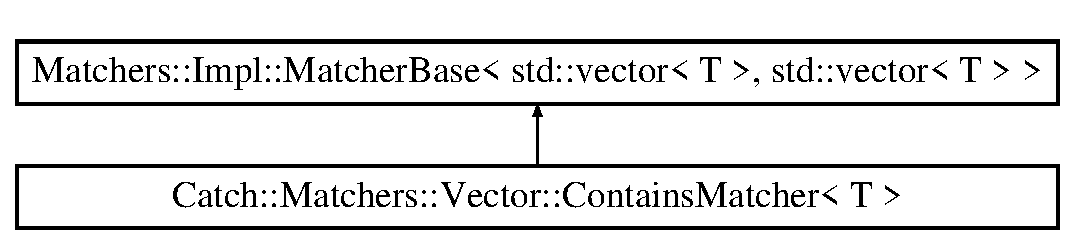
\includegraphics[height=2.000000cm]{structCatch_1_1Matchers_1_1Vector_1_1ContainsMatcher}
\end{center}
\end{figure}
\subsection*{Public Member Functions}
\begin{DoxyCompactItemize}
\item 
\hyperlink{structCatch_1_1Matchers_1_1Vector_1_1ContainsMatcher_ad8e92c8399be6dce75bb5702cdfab700}{Contains\-Matcher} (std\-::vector$<$ T $>$ const \&comparator)
\item 
bool \hyperlink{structCatch_1_1Matchers_1_1Vector_1_1ContainsMatcher_aba81516816a6796124dd4fe4843e7284}{match} (std\-::vector$<$ T $>$ const \&v) const \hyperlink{catch_8hpp_a8ecdce4d3f57835f707915ae831eb847}{C\-A\-T\-C\-H\-\_\-\-O\-V\-E\-R\-R\-I\-D\-E}
\item 
virtual std\-::string \hyperlink{structCatch_1_1Matchers_1_1Vector_1_1ContainsMatcher_add1a31f049cec89f980424ecdb7027ac}{describe} () const \hyperlink{catch_8hpp_a8ecdce4d3f57835f707915ae831eb847}{C\-A\-T\-C\-H\-\_\-\-O\-V\-E\-R\-R\-I\-D\-E}
\end{DoxyCompactItemize}
\subsection*{Public Attributes}
\begin{DoxyCompactItemize}
\item 
std\-::vector$<$ T $>$ const \& \hyperlink{structCatch_1_1Matchers_1_1Vector_1_1ContainsMatcher_a83d051166e4ed0d535219ad6ee99abb2}{m\-\_\-comparator}
\end{DoxyCompactItemize}


\subsection{Constructor \& Destructor Documentation}
\hypertarget{structCatch_1_1Matchers_1_1Vector_1_1ContainsMatcher_ad8e92c8399be6dce75bb5702cdfab700}{\index{Catch\-::\-Matchers\-::\-Vector\-::\-Contains\-Matcher@{Catch\-::\-Matchers\-::\-Vector\-::\-Contains\-Matcher}!Contains\-Matcher@{Contains\-Matcher}}
\index{Contains\-Matcher@{Contains\-Matcher}!Catch::Matchers::Vector::ContainsMatcher@{Catch\-::\-Matchers\-::\-Vector\-::\-Contains\-Matcher}}
\subsubsection[{Contains\-Matcher}]{\setlength{\rightskip}{0pt plus 5cm}template$<$typename T $>$ {\bf Catch\-::\-Matchers\-::\-Vector\-::\-Contains\-Matcher}$<$ T $>$\-::{\bf Contains\-Matcher} (
\begin{DoxyParamCaption}
\item[{std\-::vector$<$ T $>$ const \&}]{comparator}
\end{DoxyParamCaption}
)\hspace{0.3cm}{\ttfamily [inline]}}}\label{structCatch_1_1Matchers_1_1Vector_1_1ContainsMatcher_ad8e92c8399be6dce75bb5702cdfab700}


\subsection{Member Function Documentation}
\hypertarget{structCatch_1_1Matchers_1_1Vector_1_1ContainsMatcher_add1a31f049cec89f980424ecdb7027ac}{\index{Catch\-::\-Matchers\-::\-Vector\-::\-Contains\-Matcher@{Catch\-::\-Matchers\-::\-Vector\-::\-Contains\-Matcher}!describe@{describe}}
\index{describe@{describe}!Catch::Matchers::Vector::ContainsMatcher@{Catch\-::\-Matchers\-::\-Vector\-::\-Contains\-Matcher}}
\subsubsection[{describe}]{\setlength{\rightskip}{0pt plus 5cm}template$<$typename T $>$ virtual std\-::string {\bf Catch\-::\-Matchers\-::\-Vector\-::\-Contains\-Matcher}$<$ T $>$\-::describe (
\begin{DoxyParamCaption}
{}
\end{DoxyParamCaption}
) const\hspace{0.3cm}{\ttfamily [inline]}, {\ttfamily [virtual]}}}\label{structCatch_1_1Matchers_1_1Vector_1_1ContainsMatcher_add1a31f049cec89f980424ecdb7027ac}
\hypertarget{structCatch_1_1Matchers_1_1Vector_1_1ContainsMatcher_aba81516816a6796124dd4fe4843e7284}{\index{Catch\-::\-Matchers\-::\-Vector\-::\-Contains\-Matcher@{Catch\-::\-Matchers\-::\-Vector\-::\-Contains\-Matcher}!match@{match}}
\index{match@{match}!Catch::Matchers::Vector::ContainsMatcher@{Catch\-::\-Matchers\-::\-Vector\-::\-Contains\-Matcher}}
\subsubsection[{match}]{\setlength{\rightskip}{0pt plus 5cm}template$<$typename T $>$ bool {\bf Catch\-::\-Matchers\-::\-Vector\-::\-Contains\-Matcher}$<$ T $>$\-::match (
\begin{DoxyParamCaption}
\item[{std\-::vector$<$ T $>$ const \&}]{v}
\end{DoxyParamCaption}
) const\hspace{0.3cm}{\ttfamily [inline]}}}\label{structCatch_1_1Matchers_1_1Vector_1_1ContainsMatcher_aba81516816a6796124dd4fe4843e7284}


\subsection{Member Data Documentation}
\hypertarget{structCatch_1_1Matchers_1_1Vector_1_1ContainsMatcher_a83d051166e4ed0d535219ad6ee99abb2}{\index{Catch\-::\-Matchers\-::\-Vector\-::\-Contains\-Matcher@{Catch\-::\-Matchers\-::\-Vector\-::\-Contains\-Matcher}!m\-\_\-comparator@{m\-\_\-comparator}}
\index{m\-\_\-comparator@{m\-\_\-comparator}!Catch::Matchers::Vector::ContainsMatcher@{Catch\-::\-Matchers\-::\-Vector\-::\-Contains\-Matcher}}
\subsubsection[{m\-\_\-comparator}]{\setlength{\rightskip}{0pt plus 5cm}template$<$typename T $>$ std\-::vector$<$T$>$ const\& {\bf Catch\-::\-Matchers\-::\-Vector\-::\-Contains\-Matcher}$<$ T $>$\-::m\-\_\-comparator}}\label{structCatch_1_1Matchers_1_1Vector_1_1ContainsMatcher_a83d051166e4ed0d535219ad6ee99abb2}


The documentation for this struct was generated from the following file\-:\begin{DoxyCompactItemize}
\item 
/home/alexander/\-Un\-B/\-M\-P/\-Trabalho\-\_\-2\-\_\-\-M\-P\-\_\-\-Alexander\-\_\-13\-\_\-0039853/include/\hyperlink{catch_8hpp}{catch.\-hpp}\end{DoxyCompactItemize}

\hypertarget{structCatch_1_1CopyableStream}{\section{Catch\-:\-:Copyable\-Stream Struct Reference}
\label{structCatch_1_1CopyableStream}\index{Catch\-::\-Copyable\-Stream@{Catch\-::\-Copyable\-Stream}}
}


{\ttfamily \#include $<$catch.\-hpp$>$}

\subsection*{Public Member Functions}
\begin{DoxyCompactItemize}
\item 
\hyperlink{structCatch_1_1CopyableStream_a5a61d0da675ae00cd46efaef4c445cdd}{Copyable\-Stream} ()
\item 
\hyperlink{structCatch_1_1CopyableStream_a0e72dc16240653f52c17106f4bf34da8}{Copyable\-Stream} (\hyperlink{structCatch_1_1CopyableStream}{Copyable\-Stream} const \&other)
\item 
\hyperlink{structCatch_1_1CopyableStream}{Copyable\-Stream} \& \hyperlink{structCatch_1_1CopyableStream_a1760fa29b38011c5845171260bec0966}{operator=} (\hyperlink{structCatch_1_1CopyableStream}{Copyable\-Stream} const \&other)
\end{DoxyCompactItemize}
\subsection*{Public Attributes}
\begin{DoxyCompactItemize}
\item 
std\-::ostringstream \hyperlink{structCatch_1_1CopyableStream_ae123fb4d673e7d7a13a3c5f6bc5d426c}{oss}
\end{DoxyCompactItemize}


\subsection{Constructor \& Destructor Documentation}
\hypertarget{structCatch_1_1CopyableStream_a5a61d0da675ae00cd46efaef4c445cdd}{\index{Catch\-::\-Copyable\-Stream@{Catch\-::\-Copyable\-Stream}!Copyable\-Stream@{Copyable\-Stream}}
\index{Copyable\-Stream@{Copyable\-Stream}!Catch::CopyableStream@{Catch\-::\-Copyable\-Stream}}
\subsubsection[{Copyable\-Stream}]{\setlength{\rightskip}{0pt plus 5cm}Catch\-::\-Copyable\-Stream\-::\-Copyable\-Stream (
\begin{DoxyParamCaption}
{}
\end{DoxyParamCaption}
)\hspace{0.3cm}{\ttfamily [inline]}}}\label{structCatch_1_1CopyableStream_a5a61d0da675ae00cd46efaef4c445cdd}
\hypertarget{structCatch_1_1CopyableStream_a0e72dc16240653f52c17106f4bf34da8}{\index{Catch\-::\-Copyable\-Stream@{Catch\-::\-Copyable\-Stream}!Copyable\-Stream@{Copyable\-Stream}}
\index{Copyable\-Stream@{Copyable\-Stream}!Catch::CopyableStream@{Catch\-::\-Copyable\-Stream}}
\subsubsection[{Copyable\-Stream}]{\setlength{\rightskip}{0pt plus 5cm}Catch\-::\-Copyable\-Stream\-::\-Copyable\-Stream (
\begin{DoxyParamCaption}
\item[{{\bf Copyable\-Stream} const \&}]{other}
\end{DoxyParamCaption}
)\hspace{0.3cm}{\ttfamily [inline]}}}\label{structCatch_1_1CopyableStream_a0e72dc16240653f52c17106f4bf34da8}


\subsection{Member Function Documentation}
\hypertarget{structCatch_1_1CopyableStream_a1760fa29b38011c5845171260bec0966}{\index{Catch\-::\-Copyable\-Stream@{Catch\-::\-Copyable\-Stream}!operator=@{operator=}}
\index{operator=@{operator=}!Catch::CopyableStream@{Catch\-::\-Copyable\-Stream}}
\subsubsection[{operator=}]{\setlength{\rightskip}{0pt plus 5cm}{\bf Copyable\-Stream}\& Catch\-::\-Copyable\-Stream\-::operator= (
\begin{DoxyParamCaption}
\item[{{\bf Copyable\-Stream} const \&}]{other}
\end{DoxyParamCaption}
)\hspace{0.3cm}{\ttfamily [inline]}}}\label{structCatch_1_1CopyableStream_a1760fa29b38011c5845171260bec0966}


\subsection{Member Data Documentation}
\hypertarget{structCatch_1_1CopyableStream_ae123fb4d673e7d7a13a3c5f6bc5d426c}{\index{Catch\-::\-Copyable\-Stream@{Catch\-::\-Copyable\-Stream}!oss@{oss}}
\index{oss@{oss}!Catch::CopyableStream@{Catch\-::\-Copyable\-Stream}}
\subsubsection[{oss}]{\setlength{\rightskip}{0pt plus 5cm}std\-::ostringstream Catch\-::\-Copyable\-Stream\-::oss}}\label{structCatch_1_1CopyableStream_ae123fb4d673e7d7a13a3c5f6bc5d426c}


The documentation for this struct was generated from the following file\-:\begin{DoxyCompactItemize}
\item 
/home/alexander/\-Un\-B/\-M\-P/\-Trabalho\-\_\-2\-\_\-\-M\-P\-\_\-\-Alexander\-\_\-13\-\_\-0039853/include/\hyperlink{catch_8hpp}{catch.\-hpp}\end{DoxyCompactItemize}

\hypertarget{structCatch_1_1Counts}{\section{Catch\-:\-:Counts Struct Reference}
\label{structCatch_1_1Counts}\index{Catch\-::\-Counts@{Catch\-::\-Counts}}
}


{\ttfamily \#include $<$catch.\-hpp$>$}

\subsection*{Public Member Functions}
\begin{DoxyCompactItemize}
\item 
\hyperlink{structCatch_1_1Counts_aab9092ce70d4b0179cc743555d2fc39b}{Counts} ()
\item 
\hyperlink{structCatch_1_1Counts}{Counts} \hyperlink{structCatch_1_1Counts_aedf86fefe33938d132a6981171cd83e6}{operator-\/} (\hyperlink{structCatch_1_1Counts}{Counts} const \&other) const 
\item 
\hyperlink{structCatch_1_1Counts}{Counts} \& \hyperlink{structCatch_1_1Counts_a322a89475cd2cc039140ef371e973677}{operator+=} (\hyperlink{structCatch_1_1Counts}{Counts} const \&other)
\item 
std\-::size\-\_\-t \hyperlink{structCatch_1_1Counts_a9125c662e30114e5c5cc94729b1e9e84}{total} () const 
\item 
bool \hyperlink{structCatch_1_1Counts_adbbaca552f6017ce69e0d5dc5500bea4}{all\-Passed} () const 
\item 
bool \hyperlink{structCatch_1_1Counts_ab2497c9dfc77be757a90225ea69595f5}{all\-Ok} () const 
\end{DoxyCompactItemize}
\subsection*{Public Attributes}
\begin{DoxyCompactItemize}
\item 
std\-::size\-\_\-t \hyperlink{structCatch_1_1Counts_ad28daaf3de28006400208b6dd0c631e6}{passed}
\item 
std\-::size\-\_\-t \hyperlink{structCatch_1_1Counts_a19982a3817a3bc2c07f0290e71f497a3}{failed}
\item 
std\-::size\-\_\-t \hyperlink{structCatch_1_1Counts_ac090973a2ff51394cd452718e75c073e}{failed\-But\-Ok}
\end{DoxyCompactItemize}


\subsection{Constructor \& Destructor Documentation}
\hypertarget{structCatch_1_1Counts_aab9092ce70d4b0179cc743555d2fc39b}{\index{Catch\-::\-Counts@{Catch\-::\-Counts}!Counts@{Counts}}
\index{Counts@{Counts}!Catch::Counts@{Catch\-::\-Counts}}
\subsubsection[{Counts}]{\setlength{\rightskip}{0pt plus 5cm}Catch\-::\-Counts\-::\-Counts (
\begin{DoxyParamCaption}
{}
\end{DoxyParamCaption}
)\hspace{0.3cm}{\ttfamily [inline]}}}\label{structCatch_1_1Counts_aab9092ce70d4b0179cc743555d2fc39b}


\subsection{Member Function Documentation}
\hypertarget{structCatch_1_1Counts_ab2497c9dfc77be757a90225ea69595f5}{\index{Catch\-::\-Counts@{Catch\-::\-Counts}!all\-Ok@{all\-Ok}}
\index{all\-Ok@{all\-Ok}!Catch::Counts@{Catch\-::\-Counts}}
\subsubsection[{all\-Ok}]{\setlength{\rightskip}{0pt plus 5cm}bool Catch\-::\-Counts\-::all\-Ok (
\begin{DoxyParamCaption}
{}
\end{DoxyParamCaption}
) const\hspace{0.3cm}{\ttfamily [inline]}}}\label{structCatch_1_1Counts_ab2497c9dfc77be757a90225ea69595f5}
\hypertarget{structCatch_1_1Counts_adbbaca552f6017ce69e0d5dc5500bea4}{\index{Catch\-::\-Counts@{Catch\-::\-Counts}!all\-Passed@{all\-Passed}}
\index{all\-Passed@{all\-Passed}!Catch::Counts@{Catch\-::\-Counts}}
\subsubsection[{all\-Passed}]{\setlength{\rightskip}{0pt plus 5cm}bool Catch\-::\-Counts\-::all\-Passed (
\begin{DoxyParamCaption}
{}
\end{DoxyParamCaption}
) const\hspace{0.3cm}{\ttfamily [inline]}}}\label{structCatch_1_1Counts_adbbaca552f6017ce69e0d5dc5500bea4}
\hypertarget{structCatch_1_1Counts_a322a89475cd2cc039140ef371e973677}{\index{Catch\-::\-Counts@{Catch\-::\-Counts}!operator+=@{operator+=}}
\index{operator+=@{operator+=}!Catch::Counts@{Catch\-::\-Counts}}
\subsubsection[{operator+=}]{\setlength{\rightskip}{0pt plus 5cm}{\bf Counts}\& Catch\-::\-Counts\-::operator+= (
\begin{DoxyParamCaption}
\item[{{\bf Counts} const \&}]{other}
\end{DoxyParamCaption}
)\hspace{0.3cm}{\ttfamily [inline]}}}\label{structCatch_1_1Counts_a322a89475cd2cc039140ef371e973677}
\hypertarget{structCatch_1_1Counts_aedf86fefe33938d132a6981171cd83e6}{\index{Catch\-::\-Counts@{Catch\-::\-Counts}!operator-\/@{operator-\/}}
\index{operator-\/@{operator-\/}!Catch::Counts@{Catch\-::\-Counts}}
\subsubsection[{operator-\/}]{\setlength{\rightskip}{0pt plus 5cm}{\bf Counts} Catch\-::\-Counts\-::operator-\/ (
\begin{DoxyParamCaption}
\item[{{\bf Counts} const \&}]{other}
\end{DoxyParamCaption}
) const\hspace{0.3cm}{\ttfamily [inline]}}}\label{structCatch_1_1Counts_aedf86fefe33938d132a6981171cd83e6}
\hypertarget{structCatch_1_1Counts_a9125c662e30114e5c5cc94729b1e9e84}{\index{Catch\-::\-Counts@{Catch\-::\-Counts}!total@{total}}
\index{total@{total}!Catch::Counts@{Catch\-::\-Counts}}
\subsubsection[{total}]{\setlength{\rightskip}{0pt plus 5cm}std\-::size\-\_\-t Catch\-::\-Counts\-::total (
\begin{DoxyParamCaption}
{}
\end{DoxyParamCaption}
) const\hspace{0.3cm}{\ttfamily [inline]}}}\label{structCatch_1_1Counts_a9125c662e30114e5c5cc94729b1e9e84}


\subsection{Member Data Documentation}
\hypertarget{structCatch_1_1Counts_a19982a3817a3bc2c07f0290e71f497a3}{\index{Catch\-::\-Counts@{Catch\-::\-Counts}!failed@{failed}}
\index{failed@{failed}!Catch::Counts@{Catch\-::\-Counts}}
\subsubsection[{failed}]{\setlength{\rightskip}{0pt plus 5cm}std\-::size\-\_\-t Catch\-::\-Counts\-::failed}}\label{structCatch_1_1Counts_a19982a3817a3bc2c07f0290e71f497a3}
\hypertarget{structCatch_1_1Counts_ac090973a2ff51394cd452718e75c073e}{\index{Catch\-::\-Counts@{Catch\-::\-Counts}!failed\-But\-Ok@{failed\-But\-Ok}}
\index{failed\-But\-Ok@{failed\-But\-Ok}!Catch::Counts@{Catch\-::\-Counts}}
\subsubsection[{failed\-But\-Ok}]{\setlength{\rightskip}{0pt plus 5cm}std\-::size\-\_\-t Catch\-::\-Counts\-::failed\-But\-Ok}}\label{structCatch_1_1Counts_ac090973a2ff51394cd452718e75c073e}
\hypertarget{structCatch_1_1Counts_ad28daaf3de28006400208b6dd0c631e6}{\index{Catch\-::\-Counts@{Catch\-::\-Counts}!passed@{passed}}
\index{passed@{passed}!Catch::Counts@{Catch\-::\-Counts}}
\subsubsection[{passed}]{\setlength{\rightskip}{0pt plus 5cm}std\-::size\-\_\-t Catch\-::\-Counts\-::passed}}\label{structCatch_1_1Counts_ad28daaf3de28006400208b6dd0c631e6}


The documentation for this struct was generated from the following file\-:\begin{DoxyCompactItemize}
\item 
/home/alexander/\-Un\-B/\-M\-P/\-Trabalho\-\_\-2\-\_\-\-M\-P\-\_\-\-Alexander\-\_\-13\-\_\-0039853/include/\hyperlink{catch_8hpp}{catch.\-hpp}\end{DoxyCompactItemize}

\hypertarget{structCatch_1_1DecomposedExpression}{\section{Catch\-:\-:Decomposed\-Expression Struct Reference}
\label{structCatch_1_1DecomposedExpression}\index{Catch\-::\-Decomposed\-Expression@{Catch\-::\-Decomposed\-Expression}}
}


{\ttfamily \#include $<$catch.\-hpp$>$}

Inheritance diagram for Catch\-:\-:Decomposed\-Expression\-:\begin{figure}[H]
\begin{center}
\leavevmode
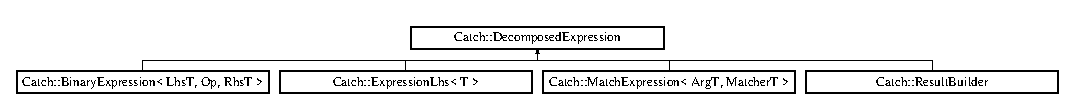
\includegraphics[height=1.029412cm]{structCatch_1_1DecomposedExpression}
\end{center}
\end{figure}
\subsection*{Public Member Functions}
\begin{DoxyCompactItemize}
\item 
virtual \hyperlink{structCatch_1_1DecomposedExpression_aa627c69bd83582c33a4d4dcac403936c}{$\sim$\-Decomposed\-Expression} ()
\item 
virtual bool \hyperlink{structCatch_1_1DecomposedExpression_af08ea5b188f04b0f441d8e4cdc340452}{is\-Binary\-Expression} () const 
\item 
virtual void \hyperlink{structCatch_1_1DecomposedExpression_a9ce7f356dc96f11f80e40c82f5aa7e55}{reconstruct\-Expression} (std\-::string \&dest) const =0
\item 
{\footnotesize template$<$typename T $>$ }\\S\-T\-A\-T\-I\-C\-\_\-\-A\-S\-S\-E\-R\-T\-\_\-\-Expression\-\_\-\-Too\-\_\-\-Complex\-\_\-\-Please\-\_\-\-Rewrite\-\_\-\-As\-\_\-\-Binary\-\_\-\-Comparison \& \hyperlink{structCatch_1_1DecomposedExpression_aa2ce96ce31fef4afb21861bc0276edb9}{operator+} (T const \&)
\item 
{\footnotesize template$<$typename T $>$ }\\S\-T\-A\-T\-I\-C\-\_\-\-A\-S\-S\-E\-R\-T\-\_\-\-Expression\-\_\-\-Too\-\_\-\-Complex\-\_\-\-Please\-\_\-\-Rewrite\-\_\-\-As\-\_\-\-Binary\-\_\-\-Comparison \& \hyperlink{structCatch_1_1DecomposedExpression_aff39fb5d060abbd018c83b998d32c366}{operator-\/} (T const \&)
\item 
{\footnotesize template$<$typename T $>$ }\\S\-T\-A\-T\-I\-C\-\_\-\-A\-S\-S\-E\-R\-T\-\_\-\-Expression\-\_\-\-Too\-\_\-\-Complex\-\_\-\-Please\-\_\-\-Rewrite\-\_\-\-As\-\_\-\-Binary\-\_\-\-Comparison \& \hyperlink{structCatch_1_1DecomposedExpression_afb5527e8e3cb8edca5113ec9801249d8}{operator$\ast$} (T const \&)
\item 
{\footnotesize template$<$typename T $>$ }\\S\-T\-A\-T\-I\-C\-\_\-\-A\-S\-S\-E\-R\-T\-\_\-\-Expression\-\_\-\-Too\-\_\-\-Complex\-\_\-\-Please\-\_\-\-Rewrite\-\_\-\-As\-\_\-\-Binary\-\_\-\-Comparison \& \hyperlink{structCatch_1_1DecomposedExpression_a519d7e2363a92106e46371c9c04044a7}{operator/} (T const \&)
\item 
{\footnotesize template$<$typename T $>$ }\\S\-T\-A\-T\-I\-C\-\_\-\-A\-S\-S\-E\-R\-T\-\_\-\-Expression\-\_\-\-Too\-\_\-\-Complex\-\_\-\-Please\-\_\-\-Rewrite\-\_\-\-As\-\_\-\-Binary\-\_\-\-Comparison \& \hyperlink{structCatch_1_1DecomposedExpression_a6584335aadaee847c9d06ca8f13a4477}{operator\%} (T const \&)
\item 
{\footnotesize template$<$typename T $>$ }\\S\-T\-A\-T\-I\-C\-\_\-\-A\-S\-S\-E\-R\-T\-\_\-\-Expression\-\_\-\-Too\-\_\-\-Complex\-\_\-\-Please\-\_\-\-Rewrite\-\_\-\-As\-\_\-\-Binary\-\_\-\-Comparison \& \hyperlink{structCatch_1_1DecomposedExpression_a63cc26b2f8bce9d4cdb5e64ef6344d7e}{operator\&\&} (T const \&)
\item 
{\footnotesize template$<$typename T $>$ }\\S\-T\-A\-T\-I\-C\-\_\-\-A\-S\-S\-E\-R\-T\-\_\-\-Expression\-\_\-\-Too\-\_\-\-Complex\-\_\-\-Please\-\_\-\-Rewrite\-\_\-\-As\-\_\-\-Binary\-\_\-\-Comparison \& \hyperlink{structCatch_1_1DecomposedExpression_ab4800d277290088fea9c594cfdd4f1c7}{operator$\vert$$\vert$} (T const \&)
\end{DoxyCompactItemize}


\subsection{Constructor \& Destructor Documentation}
\hypertarget{structCatch_1_1DecomposedExpression_aa627c69bd83582c33a4d4dcac403936c}{\index{Catch\-::\-Decomposed\-Expression@{Catch\-::\-Decomposed\-Expression}!$\sim$\-Decomposed\-Expression@{$\sim$\-Decomposed\-Expression}}
\index{$\sim$\-Decomposed\-Expression@{$\sim$\-Decomposed\-Expression}!Catch::DecomposedExpression@{Catch\-::\-Decomposed\-Expression}}
\subsubsection[{$\sim$\-Decomposed\-Expression}]{\setlength{\rightskip}{0pt plus 5cm}virtual Catch\-::\-Decomposed\-Expression\-::$\sim$\-Decomposed\-Expression (
\begin{DoxyParamCaption}
{}
\end{DoxyParamCaption}
)\hspace{0.3cm}{\ttfamily [inline]}, {\ttfamily [virtual]}}}\label{structCatch_1_1DecomposedExpression_aa627c69bd83582c33a4d4dcac403936c}


\subsection{Member Function Documentation}
\hypertarget{structCatch_1_1DecomposedExpression_af08ea5b188f04b0f441d8e4cdc340452}{\index{Catch\-::\-Decomposed\-Expression@{Catch\-::\-Decomposed\-Expression}!is\-Binary\-Expression@{is\-Binary\-Expression}}
\index{is\-Binary\-Expression@{is\-Binary\-Expression}!Catch::DecomposedExpression@{Catch\-::\-Decomposed\-Expression}}
\subsubsection[{is\-Binary\-Expression}]{\setlength{\rightskip}{0pt plus 5cm}virtual bool Catch\-::\-Decomposed\-Expression\-::is\-Binary\-Expression (
\begin{DoxyParamCaption}
{}
\end{DoxyParamCaption}
) const\hspace{0.3cm}{\ttfamily [inline]}, {\ttfamily [virtual]}}}\label{structCatch_1_1DecomposedExpression_af08ea5b188f04b0f441d8e4cdc340452}


Reimplemented in \hyperlink{classCatch_1_1MatchExpression_ac4edf6e9a6e5762a487db1486d0d1f45}{Catch\-::\-Match\-Expression$<$ Arg\-T, Matcher\-T $>$}, and \hyperlink{classCatch_1_1BinaryExpression_a4c617c0b6a73a9cafbbf900909c7c258}{Catch\-::\-Binary\-Expression$<$ Lhs\-T, Op, Rhs\-T $>$}.

\hypertarget{structCatch_1_1DecomposedExpression_a6584335aadaee847c9d06ca8f13a4477}{\index{Catch\-::\-Decomposed\-Expression@{Catch\-::\-Decomposed\-Expression}!operator\%@{operator\%}}
\index{operator\%@{operator\%}!Catch::DecomposedExpression@{Catch\-::\-Decomposed\-Expression}}
\subsubsection[{operator\%}]{\setlength{\rightskip}{0pt plus 5cm}template$<$typename T $>$ S\-T\-A\-T\-I\-C\-\_\-\-A\-S\-S\-E\-R\-T\-\_\-\-Expression\-\_\-\-Too\-\_\-\-Complex\-\_\-\-Please\-\_\-\-Rewrite\-\_\-\-As\-\_\-\-Binary\-\_\-\-Comparison\& Catch\-::\-Decomposed\-Expression\-::operator\% (
\begin{DoxyParamCaption}
\item[{T const \&}]{}
\end{DoxyParamCaption}
)}}\label{structCatch_1_1DecomposedExpression_a6584335aadaee847c9d06ca8f13a4477}
\hypertarget{structCatch_1_1DecomposedExpression_a63cc26b2f8bce9d4cdb5e64ef6344d7e}{\index{Catch\-::\-Decomposed\-Expression@{Catch\-::\-Decomposed\-Expression}!operator\&\&@{operator\&\&}}
\index{operator\&\&@{operator\&\&}!Catch::DecomposedExpression@{Catch\-::\-Decomposed\-Expression}}
\subsubsection[{operator\&\&}]{\setlength{\rightskip}{0pt plus 5cm}template$<$typename T $>$ S\-T\-A\-T\-I\-C\-\_\-\-A\-S\-S\-E\-R\-T\-\_\-\-Expression\-\_\-\-Too\-\_\-\-Complex\-\_\-\-Please\-\_\-\-Rewrite\-\_\-\-As\-\_\-\-Binary\-\_\-\-Comparison\& Catch\-::\-Decomposed\-Expression\-::operator\&\& (
\begin{DoxyParamCaption}
\item[{T const \&}]{}
\end{DoxyParamCaption}
)}}\label{structCatch_1_1DecomposedExpression_a63cc26b2f8bce9d4cdb5e64ef6344d7e}
\hypertarget{structCatch_1_1DecomposedExpression_afb5527e8e3cb8edca5113ec9801249d8}{\index{Catch\-::\-Decomposed\-Expression@{Catch\-::\-Decomposed\-Expression}!operator$\ast$@{operator$\ast$}}
\index{operator$\ast$@{operator$\ast$}!Catch::DecomposedExpression@{Catch\-::\-Decomposed\-Expression}}
\subsubsection[{operator$\ast$}]{\setlength{\rightskip}{0pt plus 5cm}template$<$typename T $>$ S\-T\-A\-T\-I\-C\-\_\-\-A\-S\-S\-E\-R\-T\-\_\-\-Expression\-\_\-\-Too\-\_\-\-Complex\-\_\-\-Please\-\_\-\-Rewrite\-\_\-\-As\-\_\-\-Binary\-\_\-\-Comparison\& Catch\-::\-Decomposed\-Expression\-::operator$\ast$ (
\begin{DoxyParamCaption}
\item[{T const \&}]{}
\end{DoxyParamCaption}
)}}\label{structCatch_1_1DecomposedExpression_afb5527e8e3cb8edca5113ec9801249d8}
\hypertarget{structCatch_1_1DecomposedExpression_aa2ce96ce31fef4afb21861bc0276edb9}{\index{Catch\-::\-Decomposed\-Expression@{Catch\-::\-Decomposed\-Expression}!operator+@{operator+}}
\index{operator+@{operator+}!Catch::DecomposedExpression@{Catch\-::\-Decomposed\-Expression}}
\subsubsection[{operator+}]{\setlength{\rightskip}{0pt plus 5cm}template$<$typename T $>$ S\-T\-A\-T\-I\-C\-\_\-\-A\-S\-S\-E\-R\-T\-\_\-\-Expression\-\_\-\-Too\-\_\-\-Complex\-\_\-\-Please\-\_\-\-Rewrite\-\_\-\-As\-\_\-\-Binary\-\_\-\-Comparison\& Catch\-::\-Decomposed\-Expression\-::operator+ (
\begin{DoxyParamCaption}
\item[{T const \&}]{}
\end{DoxyParamCaption}
)}}\label{structCatch_1_1DecomposedExpression_aa2ce96ce31fef4afb21861bc0276edb9}
\hypertarget{structCatch_1_1DecomposedExpression_aff39fb5d060abbd018c83b998d32c366}{\index{Catch\-::\-Decomposed\-Expression@{Catch\-::\-Decomposed\-Expression}!operator-\/@{operator-\/}}
\index{operator-\/@{operator-\/}!Catch::DecomposedExpression@{Catch\-::\-Decomposed\-Expression}}
\subsubsection[{operator-\/}]{\setlength{\rightskip}{0pt plus 5cm}template$<$typename T $>$ S\-T\-A\-T\-I\-C\-\_\-\-A\-S\-S\-E\-R\-T\-\_\-\-Expression\-\_\-\-Too\-\_\-\-Complex\-\_\-\-Please\-\_\-\-Rewrite\-\_\-\-As\-\_\-\-Binary\-\_\-\-Comparison\& Catch\-::\-Decomposed\-Expression\-::operator-\/ (
\begin{DoxyParamCaption}
\item[{T const \&}]{}
\end{DoxyParamCaption}
)}}\label{structCatch_1_1DecomposedExpression_aff39fb5d060abbd018c83b998d32c366}
\hypertarget{structCatch_1_1DecomposedExpression_a519d7e2363a92106e46371c9c04044a7}{\index{Catch\-::\-Decomposed\-Expression@{Catch\-::\-Decomposed\-Expression}!operator/@{operator/}}
\index{operator/@{operator/}!Catch::DecomposedExpression@{Catch\-::\-Decomposed\-Expression}}
\subsubsection[{operator/}]{\setlength{\rightskip}{0pt plus 5cm}template$<$typename T $>$ S\-T\-A\-T\-I\-C\-\_\-\-A\-S\-S\-E\-R\-T\-\_\-\-Expression\-\_\-\-Too\-\_\-\-Complex\-\_\-\-Please\-\_\-\-Rewrite\-\_\-\-As\-\_\-\-Binary\-\_\-\-Comparison\& Catch\-::\-Decomposed\-Expression\-::operator/ (
\begin{DoxyParamCaption}
\item[{T const \&}]{}
\end{DoxyParamCaption}
)}}\label{structCatch_1_1DecomposedExpression_a519d7e2363a92106e46371c9c04044a7}
\hypertarget{structCatch_1_1DecomposedExpression_ab4800d277290088fea9c594cfdd4f1c7}{\index{Catch\-::\-Decomposed\-Expression@{Catch\-::\-Decomposed\-Expression}!operator$\vert$$\vert$@{operator$\vert$$\vert$}}
\index{operator$\vert$$\vert$@{operator$\vert$$\vert$}!Catch::DecomposedExpression@{Catch\-::\-Decomposed\-Expression}}
\subsubsection[{operator$\vert$$\vert$}]{\setlength{\rightskip}{0pt plus 5cm}template$<$typename T $>$ S\-T\-A\-T\-I\-C\-\_\-\-A\-S\-S\-E\-R\-T\-\_\-\-Expression\-\_\-\-Too\-\_\-\-Complex\-\_\-\-Please\-\_\-\-Rewrite\-\_\-\-As\-\_\-\-Binary\-\_\-\-Comparison\& Catch\-::\-Decomposed\-Expression\-::operator$\vert$$\vert$ (
\begin{DoxyParamCaption}
\item[{T const \&}]{}
\end{DoxyParamCaption}
)}}\label{structCatch_1_1DecomposedExpression_ab4800d277290088fea9c594cfdd4f1c7}
\hypertarget{structCatch_1_1DecomposedExpression_a9ce7f356dc96f11f80e40c82f5aa7e55}{\index{Catch\-::\-Decomposed\-Expression@{Catch\-::\-Decomposed\-Expression}!reconstruct\-Expression@{reconstruct\-Expression}}
\index{reconstruct\-Expression@{reconstruct\-Expression}!Catch::DecomposedExpression@{Catch\-::\-Decomposed\-Expression}}
\subsubsection[{reconstruct\-Expression}]{\setlength{\rightskip}{0pt plus 5cm}virtual void Catch\-::\-Decomposed\-Expression\-::reconstruct\-Expression (
\begin{DoxyParamCaption}
\item[{std\-::string \&}]{dest}
\end{DoxyParamCaption}
) const\hspace{0.3cm}{\ttfamily [pure virtual]}}}\label{structCatch_1_1DecomposedExpression_a9ce7f356dc96f11f80e40c82f5aa7e55}


Implemented in \hyperlink{classCatch_1_1MatchExpression_a4410a93bc5b8241eb2502f400fce7ec4}{Catch\-::\-Match\-Expression$<$ Arg\-T, Matcher\-T $>$}, \hyperlink{classCatch_1_1BinaryExpression_a6ed73ff9af9c229f9fa3d35d019f9e37}{Catch\-::\-Binary\-Expression$<$ Lhs\-T, Op, Rhs\-T $>$}, \hyperlink{classCatch_1_1ExpressionLhs_a7684a053e8e88a4be475a536252630da}{Catch\-::\-Expression\-Lhs$<$ T $>$}, and \hyperlink{classCatch_1_1ResultBuilder_a7d94b15cf04301a8617e7b16158b5d82}{Catch\-::\-Result\-Builder}.



The documentation for this struct was generated from the following file\-:\begin{DoxyCompactItemize}
\item 
/home/alexander/\-Un\-B/\-M\-P/\-Trabalho\-\_\-2\-\_\-\-M\-P\-\_\-\-Alexander\-\_\-13\-\_\-0039853/include/\hyperlink{catch_8hpp}{catch.\-hpp}\end{DoxyCompactItemize}

\hypertarget{structCatch_1_1Matchers_1_1StdString_1_1EndsWithMatcher}{\section{Catch\-:\-:Matchers\-:\-:Std\-String\-:\-:Ends\-With\-Matcher Struct Reference}
\label{structCatch_1_1Matchers_1_1StdString_1_1EndsWithMatcher}\index{Catch\-::\-Matchers\-::\-Std\-String\-::\-Ends\-With\-Matcher@{Catch\-::\-Matchers\-::\-Std\-String\-::\-Ends\-With\-Matcher}}
}


{\ttfamily \#include $<$catch.\-hpp$>$}

Inheritance diagram for Catch\-:\-:Matchers\-:\-:Std\-String\-:\-:Ends\-With\-Matcher\-:\begin{figure}[H]
\begin{center}
\leavevmode
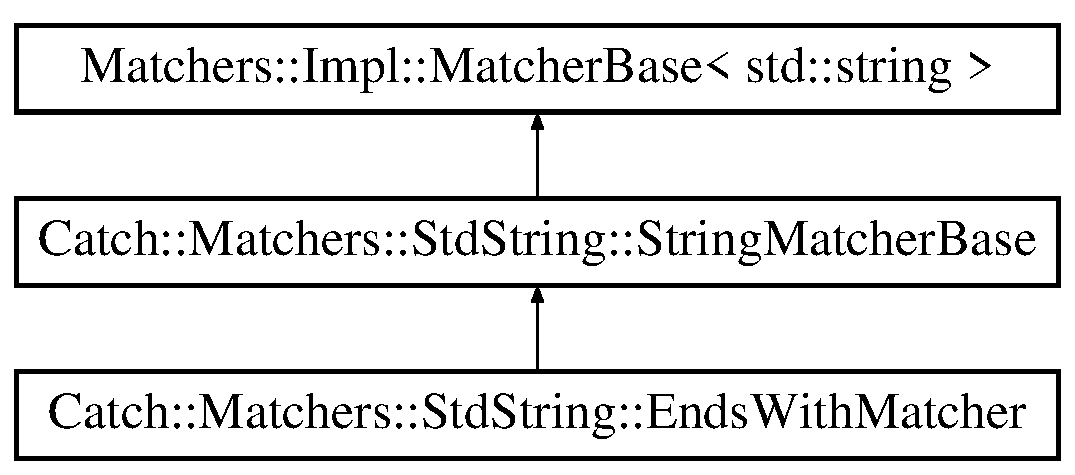
\includegraphics[height=3.000000cm]{structCatch_1_1Matchers_1_1StdString_1_1EndsWithMatcher}
\end{center}
\end{figure}
\subsection*{Public Member Functions}
\begin{DoxyCompactItemize}
\item 
\hyperlink{structCatch_1_1Matchers_1_1StdString_1_1EndsWithMatcher_aa5ec700b4629562f74f362080accfd7b}{Ends\-With\-Matcher} (\hyperlink{structCatch_1_1Matchers_1_1StdString_1_1CasedString}{Cased\-String} const \&comparator)
\item 
virtual bool \hyperlink{structCatch_1_1Matchers_1_1StdString_1_1EndsWithMatcher_a21c6dc68e30716d5c718f4f8c3186af1}{match} (std\-::string const \&source) const \hyperlink{catch_8hpp_a8ecdce4d3f57835f707915ae831eb847}{C\-A\-T\-C\-H\-\_\-\-O\-V\-E\-R\-R\-I\-D\-E}
\end{DoxyCompactItemize}
\subsection*{Additional Inherited Members}


\subsection{Constructor \& Destructor Documentation}
\hypertarget{structCatch_1_1Matchers_1_1StdString_1_1EndsWithMatcher_aa5ec700b4629562f74f362080accfd7b}{\index{Catch\-::\-Matchers\-::\-Std\-String\-::\-Ends\-With\-Matcher@{Catch\-::\-Matchers\-::\-Std\-String\-::\-Ends\-With\-Matcher}!Ends\-With\-Matcher@{Ends\-With\-Matcher}}
\index{Ends\-With\-Matcher@{Ends\-With\-Matcher}!Catch::Matchers::StdString::EndsWithMatcher@{Catch\-::\-Matchers\-::\-Std\-String\-::\-Ends\-With\-Matcher}}
\subsubsection[{Ends\-With\-Matcher}]{\setlength{\rightskip}{0pt plus 5cm}Catch\-::\-Matchers\-::\-Std\-String\-::\-Ends\-With\-Matcher\-::\-Ends\-With\-Matcher (
\begin{DoxyParamCaption}
\item[{{\bf Cased\-String} const \&}]{comparator}
\end{DoxyParamCaption}
)}}\label{structCatch_1_1Matchers_1_1StdString_1_1EndsWithMatcher_aa5ec700b4629562f74f362080accfd7b}


\subsection{Member Function Documentation}
\hypertarget{structCatch_1_1Matchers_1_1StdString_1_1EndsWithMatcher_a21c6dc68e30716d5c718f4f8c3186af1}{\index{Catch\-::\-Matchers\-::\-Std\-String\-::\-Ends\-With\-Matcher@{Catch\-::\-Matchers\-::\-Std\-String\-::\-Ends\-With\-Matcher}!match@{match}}
\index{match@{match}!Catch::Matchers::StdString::EndsWithMatcher@{Catch\-::\-Matchers\-::\-Std\-String\-::\-Ends\-With\-Matcher}}
\subsubsection[{match}]{\setlength{\rightskip}{0pt plus 5cm}virtual bool Catch\-::\-Matchers\-::\-Std\-String\-::\-Ends\-With\-Matcher\-::match (
\begin{DoxyParamCaption}
\item[{std\-::string const \&}]{source}
\end{DoxyParamCaption}
) const\hspace{0.3cm}{\ttfamily [virtual]}}}\label{structCatch_1_1Matchers_1_1StdString_1_1EndsWithMatcher_a21c6dc68e30716d5c718f4f8c3186af1}


The documentation for this struct was generated from the following file\-:\begin{DoxyCompactItemize}
\item 
/home/alexander/\-Un\-B/\-M\-P/\-Trabalho\-\_\-2\-\_\-\-M\-P\-\_\-\-Alexander\-\_\-13\-\_\-0039853/include/\hyperlink{catch_8hpp}{catch.\-hpp}\end{DoxyCompactItemize}

\hypertarget{structCatch_1_1Matchers_1_1StdString_1_1EqualsMatcher}{\section{Catch\-:\-:Matchers\-:\-:Std\-String\-:\-:Equals\-Matcher Struct Reference}
\label{structCatch_1_1Matchers_1_1StdString_1_1EqualsMatcher}\index{Catch\-::\-Matchers\-::\-Std\-String\-::\-Equals\-Matcher@{Catch\-::\-Matchers\-::\-Std\-String\-::\-Equals\-Matcher}}
}


{\ttfamily \#include $<$catch.\-hpp$>$}

Inheritance diagram for Catch\-:\-:Matchers\-:\-:Std\-String\-:\-:Equals\-Matcher\-:\begin{figure}[H]
\begin{center}
\leavevmode
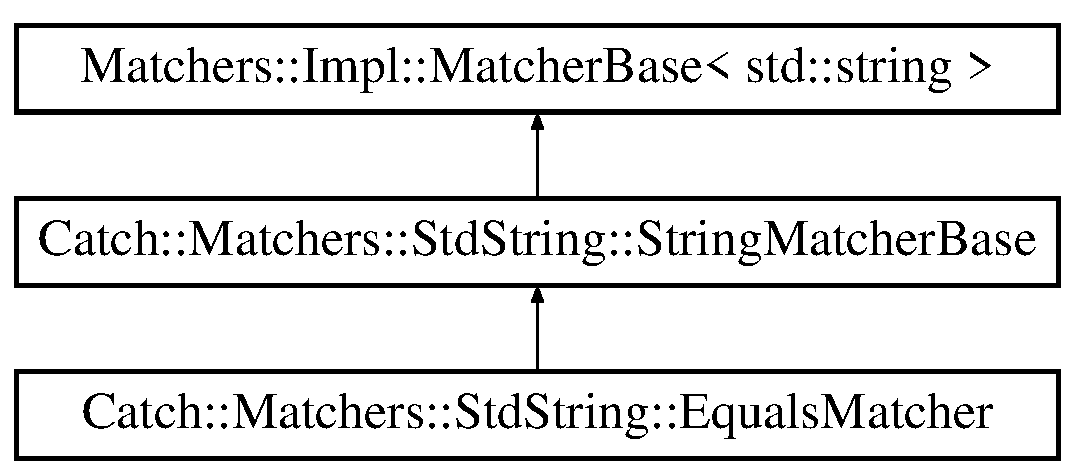
\includegraphics[height=3.000000cm]{structCatch_1_1Matchers_1_1StdString_1_1EqualsMatcher}
\end{center}
\end{figure}
\subsection*{Public Member Functions}
\begin{DoxyCompactItemize}
\item 
\hyperlink{structCatch_1_1Matchers_1_1StdString_1_1EqualsMatcher_ab740f1fb2310e9fe3fed5134d4c7e4c8}{Equals\-Matcher} (\hyperlink{structCatch_1_1Matchers_1_1StdString_1_1CasedString}{Cased\-String} const \&comparator)
\item 
virtual bool \hyperlink{structCatch_1_1Matchers_1_1StdString_1_1EqualsMatcher_a2aeaac3c0efb8422643cd1b155256213}{match} (std\-::string const \&source) const \hyperlink{catch_8hpp_a8ecdce4d3f57835f707915ae831eb847}{C\-A\-T\-C\-H\-\_\-\-O\-V\-E\-R\-R\-I\-D\-E}
\end{DoxyCompactItemize}
\subsection*{Additional Inherited Members}


\subsection{Constructor \& Destructor Documentation}
\hypertarget{structCatch_1_1Matchers_1_1StdString_1_1EqualsMatcher_ab740f1fb2310e9fe3fed5134d4c7e4c8}{\index{Catch\-::\-Matchers\-::\-Std\-String\-::\-Equals\-Matcher@{Catch\-::\-Matchers\-::\-Std\-String\-::\-Equals\-Matcher}!Equals\-Matcher@{Equals\-Matcher}}
\index{Equals\-Matcher@{Equals\-Matcher}!Catch::Matchers::StdString::EqualsMatcher@{Catch\-::\-Matchers\-::\-Std\-String\-::\-Equals\-Matcher}}
\subsubsection[{Equals\-Matcher}]{\setlength{\rightskip}{0pt plus 5cm}Catch\-::\-Matchers\-::\-Std\-String\-::\-Equals\-Matcher\-::\-Equals\-Matcher (
\begin{DoxyParamCaption}
\item[{{\bf Cased\-String} const \&}]{comparator}
\end{DoxyParamCaption}
)}}\label{structCatch_1_1Matchers_1_1StdString_1_1EqualsMatcher_ab740f1fb2310e9fe3fed5134d4c7e4c8}


\subsection{Member Function Documentation}
\hypertarget{structCatch_1_1Matchers_1_1StdString_1_1EqualsMatcher_a2aeaac3c0efb8422643cd1b155256213}{\index{Catch\-::\-Matchers\-::\-Std\-String\-::\-Equals\-Matcher@{Catch\-::\-Matchers\-::\-Std\-String\-::\-Equals\-Matcher}!match@{match}}
\index{match@{match}!Catch::Matchers::StdString::EqualsMatcher@{Catch\-::\-Matchers\-::\-Std\-String\-::\-Equals\-Matcher}}
\subsubsection[{match}]{\setlength{\rightskip}{0pt plus 5cm}virtual bool Catch\-::\-Matchers\-::\-Std\-String\-::\-Equals\-Matcher\-::match (
\begin{DoxyParamCaption}
\item[{std\-::string const \&}]{source}
\end{DoxyParamCaption}
) const\hspace{0.3cm}{\ttfamily [virtual]}}}\label{structCatch_1_1Matchers_1_1StdString_1_1EqualsMatcher_a2aeaac3c0efb8422643cd1b155256213}


The documentation for this struct was generated from the following file\-:\begin{DoxyCompactItemize}
\item 
/home/alexander/\-Un\-B/\-M\-P/\-Trabalho\-\_\-2\-\_\-\-M\-P\-\_\-\-Alexander\-\_\-13\-\_\-0039853/include/\hyperlink{catch_8hpp}{catch.\-hpp}\end{DoxyCompactItemize}

\hypertarget{structCatch_1_1Matchers_1_1Vector_1_1EqualsMatcher}{\section{Catch\-:\-:Matchers\-:\-:Vector\-:\-:Equals\-Matcher$<$ T $>$ Struct Template Reference}
\label{structCatch_1_1Matchers_1_1Vector_1_1EqualsMatcher}\index{Catch\-::\-Matchers\-::\-Vector\-::\-Equals\-Matcher$<$ T $>$@{Catch\-::\-Matchers\-::\-Vector\-::\-Equals\-Matcher$<$ T $>$}}
}


{\ttfamily \#include $<$catch.\-hpp$>$}

Inheritance diagram for Catch\-:\-:Matchers\-:\-:Vector\-:\-:Equals\-Matcher$<$ T $>$\-:\begin{figure}[H]
\begin{center}
\leavevmode
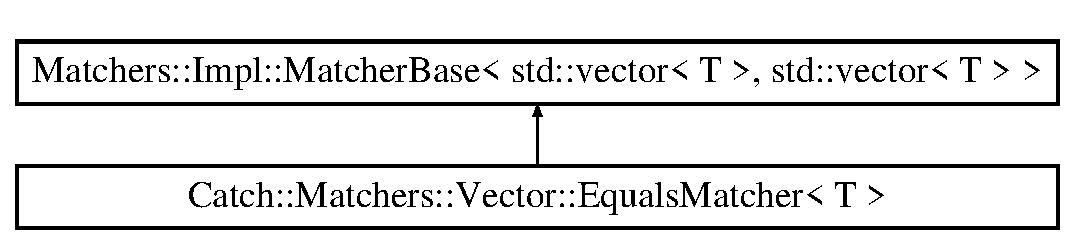
\includegraphics[height=2.000000cm]{structCatch_1_1Matchers_1_1Vector_1_1EqualsMatcher}
\end{center}
\end{figure}
\subsection*{Public Member Functions}
\begin{DoxyCompactItemize}
\item 
\hyperlink{structCatch_1_1Matchers_1_1Vector_1_1EqualsMatcher_a3846c47780d1991dcfe87aefded98008}{Equals\-Matcher} (std\-::vector$<$ T $>$ const \&comparator)
\item 
bool \hyperlink{structCatch_1_1Matchers_1_1Vector_1_1EqualsMatcher_aca444c319d1b4c6f538faf9c4735da04}{match} (std\-::vector$<$ T $>$ const \&v) const \hyperlink{catch_8hpp_a8ecdce4d3f57835f707915ae831eb847}{C\-A\-T\-C\-H\-\_\-\-O\-V\-E\-R\-R\-I\-D\-E}
\item 
virtual std\-::string \hyperlink{structCatch_1_1Matchers_1_1Vector_1_1EqualsMatcher_aca79ade26f4a75b2a57005067e086e35}{describe} () const \hyperlink{catch_8hpp_a8ecdce4d3f57835f707915ae831eb847}{C\-A\-T\-C\-H\-\_\-\-O\-V\-E\-R\-R\-I\-D\-E}
\end{DoxyCompactItemize}
\subsection*{Public Attributes}
\begin{DoxyCompactItemize}
\item 
std\-::vector$<$ T $>$ const \& \hyperlink{structCatch_1_1Matchers_1_1Vector_1_1EqualsMatcher_a56f7aa6f110a12b1b9aeb0cabbc9d755}{m\-\_\-comparator}
\end{DoxyCompactItemize}


\subsection{Constructor \& Destructor Documentation}
\hypertarget{structCatch_1_1Matchers_1_1Vector_1_1EqualsMatcher_a3846c47780d1991dcfe87aefded98008}{\index{Catch\-::\-Matchers\-::\-Vector\-::\-Equals\-Matcher@{Catch\-::\-Matchers\-::\-Vector\-::\-Equals\-Matcher}!Equals\-Matcher@{Equals\-Matcher}}
\index{Equals\-Matcher@{Equals\-Matcher}!Catch::Matchers::Vector::EqualsMatcher@{Catch\-::\-Matchers\-::\-Vector\-::\-Equals\-Matcher}}
\subsubsection[{Equals\-Matcher}]{\setlength{\rightskip}{0pt plus 5cm}template$<$typename T $>$ {\bf Catch\-::\-Matchers\-::\-Vector\-::\-Equals\-Matcher}$<$ T $>$\-::{\bf Equals\-Matcher} (
\begin{DoxyParamCaption}
\item[{std\-::vector$<$ T $>$ const \&}]{comparator}
\end{DoxyParamCaption}
)\hspace{0.3cm}{\ttfamily [inline]}}}\label{structCatch_1_1Matchers_1_1Vector_1_1EqualsMatcher_a3846c47780d1991dcfe87aefded98008}


\subsection{Member Function Documentation}
\hypertarget{structCatch_1_1Matchers_1_1Vector_1_1EqualsMatcher_aca79ade26f4a75b2a57005067e086e35}{\index{Catch\-::\-Matchers\-::\-Vector\-::\-Equals\-Matcher@{Catch\-::\-Matchers\-::\-Vector\-::\-Equals\-Matcher}!describe@{describe}}
\index{describe@{describe}!Catch::Matchers::Vector::EqualsMatcher@{Catch\-::\-Matchers\-::\-Vector\-::\-Equals\-Matcher}}
\subsubsection[{describe}]{\setlength{\rightskip}{0pt plus 5cm}template$<$typename T $>$ virtual std\-::string {\bf Catch\-::\-Matchers\-::\-Vector\-::\-Equals\-Matcher}$<$ T $>$\-::describe (
\begin{DoxyParamCaption}
{}
\end{DoxyParamCaption}
) const\hspace{0.3cm}{\ttfamily [inline]}, {\ttfamily [virtual]}}}\label{structCatch_1_1Matchers_1_1Vector_1_1EqualsMatcher_aca79ade26f4a75b2a57005067e086e35}
\hypertarget{structCatch_1_1Matchers_1_1Vector_1_1EqualsMatcher_aca444c319d1b4c6f538faf9c4735da04}{\index{Catch\-::\-Matchers\-::\-Vector\-::\-Equals\-Matcher@{Catch\-::\-Matchers\-::\-Vector\-::\-Equals\-Matcher}!match@{match}}
\index{match@{match}!Catch::Matchers::Vector::EqualsMatcher@{Catch\-::\-Matchers\-::\-Vector\-::\-Equals\-Matcher}}
\subsubsection[{match}]{\setlength{\rightskip}{0pt plus 5cm}template$<$typename T $>$ bool {\bf Catch\-::\-Matchers\-::\-Vector\-::\-Equals\-Matcher}$<$ T $>$\-::match (
\begin{DoxyParamCaption}
\item[{std\-::vector$<$ T $>$ const \&}]{v}
\end{DoxyParamCaption}
) const\hspace{0.3cm}{\ttfamily [inline]}}}\label{structCatch_1_1Matchers_1_1Vector_1_1EqualsMatcher_aca444c319d1b4c6f538faf9c4735da04}


\subsection{Member Data Documentation}
\hypertarget{structCatch_1_1Matchers_1_1Vector_1_1EqualsMatcher_a56f7aa6f110a12b1b9aeb0cabbc9d755}{\index{Catch\-::\-Matchers\-::\-Vector\-::\-Equals\-Matcher@{Catch\-::\-Matchers\-::\-Vector\-::\-Equals\-Matcher}!m\-\_\-comparator@{m\-\_\-comparator}}
\index{m\-\_\-comparator@{m\-\_\-comparator}!Catch::Matchers::Vector::EqualsMatcher@{Catch\-::\-Matchers\-::\-Vector\-::\-Equals\-Matcher}}
\subsubsection[{m\-\_\-comparator}]{\setlength{\rightskip}{0pt plus 5cm}template$<$typename T $>$ std\-::vector$<$T$>$ const\& {\bf Catch\-::\-Matchers\-::\-Vector\-::\-Equals\-Matcher}$<$ T $>$\-::m\-\_\-comparator}}\label{structCatch_1_1Matchers_1_1Vector_1_1EqualsMatcher_a56f7aa6f110a12b1b9aeb0cabbc9d755}


The documentation for this struct was generated from the following file\-:\begin{DoxyCompactItemize}
\item 
/home/alexander/\-Un\-B/\-M\-P/\-Trabalho\-\_\-2\-\_\-\-M\-P\-\_\-\-Alexander\-\_\-13\-\_\-0039853/include/\hyperlink{catch_8hpp}{catch.\-hpp}\end{DoxyCompactItemize}

\hypertarget{classCatch_1_1Internal_1_1Evaluator}{\section{Catch\-:\-:Internal\-:\-:Evaluator$<$ T1, T2, Op $>$ Class Template Reference}
\label{classCatch_1_1Internal_1_1Evaluator}\index{Catch\-::\-Internal\-::\-Evaluator$<$ T1, T2, Op $>$@{Catch\-::\-Internal\-::\-Evaluator$<$ T1, T2, Op $>$}}
}


{\ttfamily \#include $<$catch.\-hpp$>$}



The documentation for this class was generated from the following file\-:\begin{DoxyCompactItemize}
\item 
/home/alexander/\-Un\-B/\-M\-P/\-Trabalho\-\_\-2\-\_\-\-M\-P\-\_\-\-Alexander\-\_\-13\-\_\-0039853/include/\hyperlink{catch_8hpp}{catch.\-hpp}\end{DoxyCompactItemize}

\hypertarget{structCatch_1_1Internal_1_1Evaluator_3_01T1_00_01T2_00_01IsEqualTo_01_4}{\section{Catch\-:\-:Internal\-:\-:Evaluator$<$ T1, T2, Is\-Equal\-To $>$ Struct Template Reference}
\label{structCatch_1_1Internal_1_1Evaluator_3_01T1_00_01T2_00_01IsEqualTo_01_4}\index{Catch\-::\-Internal\-::\-Evaluator$<$ T1, T2, Is\-Equal\-To $>$@{Catch\-::\-Internal\-::\-Evaluator$<$ T1, T2, Is\-Equal\-To $>$}}
}


{\ttfamily \#include $<$catch.\-hpp$>$}

\subsection*{Static Public Member Functions}
\begin{DoxyCompactItemize}
\item 
static bool \hyperlink{structCatch_1_1Internal_1_1Evaluator_3_01T1_00_01T2_00_01IsEqualTo_01_4_a166b2b7849247397e63fb2940481b217}{evaluate} (T1 const \&lhs, T2 const \&rhs)
\end{DoxyCompactItemize}


\subsection{Member Function Documentation}
\hypertarget{structCatch_1_1Internal_1_1Evaluator_3_01T1_00_01T2_00_01IsEqualTo_01_4_a166b2b7849247397e63fb2940481b217}{\index{Catch\-::\-Internal\-::\-Evaluator$<$ T1, T2, Is\-Equal\-To $>$@{Catch\-::\-Internal\-::\-Evaluator$<$ T1, T2, Is\-Equal\-To $>$}!evaluate@{evaluate}}
\index{evaluate@{evaluate}!Catch::Internal::Evaluator< T1, T2, IsEqualTo >@{Catch\-::\-Internal\-::\-Evaluator$<$ T1, T2, Is\-Equal\-To $>$}}
\subsubsection[{evaluate}]{\setlength{\rightskip}{0pt plus 5cm}template$<$typename T1 , typename T2 $>$ static bool {\bf Catch\-::\-Internal\-::\-Evaluator}$<$ T1, T2, {\bf Is\-Equal\-To} $>$\-::evaluate (
\begin{DoxyParamCaption}
\item[{T1 const \&}]{lhs, }
\item[{T2 const \&}]{rhs}
\end{DoxyParamCaption}
)\hspace{0.3cm}{\ttfamily [inline]}, {\ttfamily [static]}}}\label{structCatch_1_1Internal_1_1Evaluator_3_01T1_00_01T2_00_01IsEqualTo_01_4_a166b2b7849247397e63fb2940481b217}


The documentation for this struct was generated from the following file\-:\begin{DoxyCompactItemize}
\item 
/home/alexander/\-Un\-B/\-M\-P/\-Trabalho\-\_\-2\-\_\-\-M\-P\-\_\-\-Alexander\-\_\-13\-\_\-0039853/include/\hyperlink{catch_8hpp}{catch.\-hpp}\end{DoxyCompactItemize}

\hypertarget{structCatch_1_1Internal_1_1Evaluator_3_01T1_00_01T2_00_01IsGreaterThan_01_4}{\section{Catch\-:\-:Internal\-:\-:Evaluator$<$ T1, T2, Is\-Greater\-Than $>$ Struct Template Reference}
\label{structCatch_1_1Internal_1_1Evaluator_3_01T1_00_01T2_00_01IsGreaterThan_01_4}\index{Catch\-::\-Internal\-::\-Evaluator$<$ T1, T2, Is\-Greater\-Than $>$@{Catch\-::\-Internal\-::\-Evaluator$<$ T1, T2, Is\-Greater\-Than $>$}}
}


{\ttfamily \#include $<$catch.\-hpp$>$}

\subsection*{Static Public Member Functions}
\begin{DoxyCompactItemize}
\item 
static bool \hyperlink{structCatch_1_1Internal_1_1Evaluator_3_01T1_00_01T2_00_01IsGreaterThan_01_4_a55745f74f09ac5c61bd3d592ca5560af}{evaluate} (T1 const \&lhs, T2 const \&rhs)
\end{DoxyCompactItemize}


\subsection{Member Function Documentation}
\hypertarget{structCatch_1_1Internal_1_1Evaluator_3_01T1_00_01T2_00_01IsGreaterThan_01_4_a55745f74f09ac5c61bd3d592ca5560af}{\index{Catch\-::\-Internal\-::\-Evaluator$<$ T1, T2, Is\-Greater\-Than $>$@{Catch\-::\-Internal\-::\-Evaluator$<$ T1, T2, Is\-Greater\-Than $>$}!evaluate@{evaluate}}
\index{evaluate@{evaluate}!Catch::Internal::Evaluator< T1, T2, IsGreaterThan >@{Catch\-::\-Internal\-::\-Evaluator$<$ T1, T2, Is\-Greater\-Than $>$}}
\subsubsection[{evaluate}]{\setlength{\rightskip}{0pt plus 5cm}template$<$typename T1 , typename T2 $>$ static bool {\bf Catch\-::\-Internal\-::\-Evaluator}$<$ T1, T2, {\bf Is\-Greater\-Than} $>$\-::evaluate (
\begin{DoxyParamCaption}
\item[{T1 const \&}]{lhs, }
\item[{T2 const \&}]{rhs}
\end{DoxyParamCaption}
)\hspace{0.3cm}{\ttfamily [inline]}, {\ttfamily [static]}}}\label{structCatch_1_1Internal_1_1Evaluator_3_01T1_00_01T2_00_01IsGreaterThan_01_4_a55745f74f09ac5c61bd3d592ca5560af}


The documentation for this struct was generated from the following file\-:\begin{DoxyCompactItemize}
\item 
/home/alexander/\-Un\-B/\-M\-P/\-Trabalho\-\_\-2\-\_\-\-M\-P\-\_\-\-Alexander\-\_\-13\-\_\-0039853/include/\hyperlink{catch_8hpp}{catch.\-hpp}\end{DoxyCompactItemize}

\hypertarget{structCatch_1_1Internal_1_1Evaluator_3_01T1_00_01T2_00_01IsGreaterThanOrEqualTo_01_4}{\section{Catch\-:\-:Internal\-:\-:Evaluator$<$ T1, T2, Is\-Greater\-Than\-Or\-Equal\-To $>$ Struct Template Reference}
\label{structCatch_1_1Internal_1_1Evaluator_3_01T1_00_01T2_00_01IsGreaterThanOrEqualTo_01_4}\index{Catch\-::\-Internal\-::\-Evaluator$<$ T1, T2, Is\-Greater\-Than\-Or\-Equal\-To $>$@{Catch\-::\-Internal\-::\-Evaluator$<$ T1, T2, Is\-Greater\-Than\-Or\-Equal\-To $>$}}
}


{\ttfamily \#include $<$catch.\-hpp$>$}

\subsection*{Static Public Member Functions}
\begin{DoxyCompactItemize}
\item 
static bool \hyperlink{structCatch_1_1Internal_1_1Evaluator_3_01T1_00_01T2_00_01IsGreaterThanOrEqualTo_01_4_a5ba107c6da4292b6492a0e5e906f9484}{evaluate} (T1 const \&lhs, T2 const \&rhs)
\end{DoxyCompactItemize}


\subsection{Member Function Documentation}
\hypertarget{structCatch_1_1Internal_1_1Evaluator_3_01T1_00_01T2_00_01IsGreaterThanOrEqualTo_01_4_a5ba107c6da4292b6492a0e5e906f9484}{\index{Catch\-::\-Internal\-::\-Evaluator$<$ T1, T2, Is\-Greater\-Than\-Or\-Equal\-To $>$@{Catch\-::\-Internal\-::\-Evaluator$<$ T1, T2, Is\-Greater\-Than\-Or\-Equal\-To $>$}!evaluate@{evaluate}}
\index{evaluate@{evaluate}!Catch::Internal::Evaluator< T1, T2, IsGreaterThanOrEqualTo >@{Catch\-::\-Internal\-::\-Evaluator$<$ T1, T2, Is\-Greater\-Than\-Or\-Equal\-To $>$}}
\subsubsection[{evaluate}]{\setlength{\rightskip}{0pt plus 5cm}template$<$typename T1 , typename T2 $>$ static bool {\bf Catch\-::\-Internal\-::\-Evaluator}$<$ T1, T2, {\bf Is\-Greater\-Than\-Or\-Equal\-To} $>$\-::evaluate (
\begin{DoxyParamCaption}
\item[{T1 const \&}]{lhs, }
\item[{T2 const \&}]{rhs}
\end{DoxyParamCaption}
)\hspace{0.3cm}{\ttfamily [inline]}, {\ttfamily [static]}}}\label{structCatch_1_1Internal_1_1Evaluator_3_01T1_00_01T2_00_01IsGreaterThanOrEqualTo_01_4_a5ba107c6da4292b6492a0e5e906f9484}


The documentation for this struct was generated from the following file\-:\begin{DoxyCompactItemize}
\item 
/home/alexander/\-Un\-B/\-M\-P/\-Trabalho\-\_\-2\-\_\-\-M\-P\-\_\-\-Alexander\-\_\-13\-\_\-0039853/include/\hyperlink{catch_8hpp}{catch.\-hpp}\end{DoxyCompactItemize}

\hypertarget{structCatch_1_1Internal_1_1Evaluator_3_01T1_00_01T2_00_01IsLessThan_01_4}{\section{Catch\-:\-:Internal\-:\-:Evaluator$<$ T1, T2, Is\-Less\-Than $>$ Struct Template Reference}
\label{structCatch_1_1Internal_1_1Evaluator_3_01T1_00_01T2_00_01IsLessThan_01_4}\index{Catch\-::\-Internal\-::\-Evaluator$<$ T1, T2, Is\-Less\-Than $>$@{Catch\-::\-Internal\-::\-Evaluator$<$ T1, T2, Is\-Less\-Than $>$}}
}


{\ttfamily \#include $<$catch.\-hpp$>$}

\subsection*{Static Public Member Functions}
\begin{DoxyCompactItemize}
\item 
static bool \hyperlink{structCatch_1_1Internal_1_1Evaluator_3_01T1_00_01T2_00_01IsLessThan_01_4_a75b2bcf80ce6f90218c145e2c3293d75}{evaluate} (T1 const \&lhs, T2 const \&rhs)
\end{DoxyCompactItemize}


\subsection{Member Function Documentation}
\hypertarget{structCatch_1_1Internal_1_1Evaluator_3_01T1_00_01T2_00_01IsLessThan_01_4_a75b2bcf80ce6f90218c145e2c3293d75}{\index{Catch\-::\-Internal\-::\-Evaluator$<$ T1, T2, Is\-Less\-Than $>$@{Catch\-::\-Internal\-::\-Evaluator$<$ T1, T2, Is\-Less\-Than $>$}!evaluate@{evaluate}}
\index{evaluate@{evaluate}!Catch::Internal::Evaluator< T1, T2, IsLessThan >@{Catch\-::\-Internal\-::\-Evaluator$<$ T1, T2, Is\-Less\-Than $>$}}
\subsubsection[{evaluate}]{\setlength{\rightskip}{0pt plus 5cm}template$<$typename T1 , typename T2 $>$ static bool {\bf Catch\-::\-Internal\-::\-Evaluator}$<$ T1, T2, {\bf Is\-Less\-Than} $>$\-::evaluate (
\begin{DoxyParamCaption}
\item[{T1 const \&}]{lhs, }
\item[{T2 const \&}]{rhs}
\end{DoxyParamCaption}
)\hspace{0.3cm}{\ttfamily [inline]}, {\ttfamily [static]}}}\label{structCatch_1_1Internal_1_1Evaluator_3_01T1_00_01T2_00_01IsLessThan_01_4_a75b2bcf80ce6f90218c145e2c3293d75}


The documentation for this struct was generated from the following file\-:\begin{DoxyCompactItemize}
\item 
/home/alexander/\-Un\-B/\-M\-P/\-Trabalho\-\_\-2\-\_\-\-M\-P\-\_\-\-Alexander\-\_\-13\-\_\-0039853/include/\hyperlink{catch_8hpp}{catch.\-hpp}\end{DoxyCompactItemize}

\hypertarget{structCatch_1_1Internal_1_1Evaluator_3_01T1_00_01T2_00_01IsLessThanOrEqualTo_01_4}{\section{Catch\-:\-:Internal\-:\-:Evaluator$<$ T1, T2, Is\-Less\-Than\-Or\-Equal\-To $>$ Struct Template Reference}
\label{structCatch_1_1Internal_1_1Evaluator_3_01T1_00_01T2_00_01IsLessThanOrEqualTo_01_4}\index{Catch\-::\-Internal\-::\-Evaluator$<$ T1, T2, Is\-Less\-Than\-Or\-Equal\-To $>$@{Catch\-::\-Internal\-::\-Evaluator$<$ T1, T2, Is\-Less\-Than\-Or\-Equal\-To $>$}}
}


{\ttfamily \#include $<$catch.\-hpp$>$}

\subsection*{Static Public Member Functions}
\begin{DoxyCompactItemize}
\item 
static bool \hyperlink{structCatch_1_1Internal_1_1Evaluator_3_01T1_00_01T2_00_01IsLessThanOrEqualTo_01_4_adf269a597e4d82d69f29bcb516297b9b}{evaluate} (T1 const \&lhs, T2 const \&rhs)
\end{DoxyCompactItemize}


\subsection{Member Function Documentation}
\hypertarget{structCatch_1_1Internal_1_1Evaluator_3_01T1_00_01T2_00_01IsLessThanOrEqualTo_01_4_adf269a597e4d82d69f29bcb516297b9b}{\index{Catch\-::\-Internal\-::\-Evaluator$<$ T1, T2, Is\-Less\-Than\-Or\-Equal\-To $>$@{Catch\-::\-Internal\-::\-Evaluator$<$ T1, T2, Is\-Less\-Than\-Or\-Equal\-To $>$}!evaluate@{evaluate}}
\index{evaluate@{evaluate}!Catch::Internal::Evaluator< T1, T2, IsLessThanOrEqualTo >@{Catch\-::\-Internal\-::\-Evaluator$<$ T1, T2, Is\-Less\-Than\-Or\-Equal\-To $>$}}
\subsubsection[{evaluate}]{\setlength{\rightskip}{0pt plus 5cm}template$<$typename T1 , typename T2 $>$ static bool {\bf Catch\-::\-Internal\-::\-Evaluator}$<$ T1, T2, {\bf Is\-Less\-Than\-Or\-Equal\-To} $>$\-::evaluate (
\begin{DoxyParamCaption}
\item[{T1 const \&}]{lhs, }
\item[{T2 const \&}]{rhs}
\end{DoxyParamCaption}
)\hspace{0.3cm}{\ttfamily [inline]}, {\ttfamily [static]}}}\label{structCatch_1_1Internal_1_1Evaluator_3_01T1_00_01T2_00_01IsLessThanOrEqualTo_01_4_adf269a597e4d82d69f29bcb516297b9b}


The documentation for this struct was generated from the following file\-:\begin{DoxyCompactItemize}
\item 
/home/alexander/\-Un\-B/\-M\-P/\-Trabalho\-\_\-2\-\_\-\-M\-P\-\_\-\-Alexander\-\_\-13\-\_\-0039853/include/\hyperlink{catch_8hpp}{catch.\-hpp}\end{DoxyCompactItemize}

\hypertarget{structCatch_1_1Internal_1_1Evaluator_3_01T1_00_01T2_00_01IsNotEqualTo_01_4}{\section{Catch\-:\-:Internal\-:\-:Evaluator$<$ T1, T2, Is\-Not\-Equal\-To $>$ Struct Template Reference}
\label{structCatch_1_1Internal_1_1Evaluator_3_01T1_00_01T2_00_01IsNotEqualTo_01_4}\index{Catch\-::\-Internal\-::\-Evaluator$<$ T1, T2, Is\-Not\-Equal\-To $>$@{Catch\-::\-Internal\-::\-Evaluator$<$ T1, T2, Is\-Not\-Equal\-To $>$}}
}


{\ttfamily \#include $<$catch.\-hpp$>$}

\subsection*{Static Public Member Functions}
\begin{DoxyCompactItemize}
\item 
static bool \hyperlink{structCatch_1_1Internal_1_1Evaluator_3_01T1_00_01T2_00_01IsNotEqualTo_01_4_a956a12d0f4a7dceb5a1ce914421ff945}{evaluate} (T1 const \&lhs, T2 const \&rhs)
\end{DoxyCompactItemize}


\subsection{Member Function Documentation}
\hypertarget{structCatch_1_1Internal_1_1Evaluator_3_01T1_00_01T2_00_01IsNotEqualTo_01_4_a956a12d0f4a7dceb5a1ce914421ff945}{\index{Catch\-::\-Internal\-::\-Evaluator$<$ T1, T2, Is\-Not\-Equal\-To $>$@{Catch\-::\-Internal\-::\-Evaluator$<$ T1, T2, Is\-Not\-Equal\-To $>$}!evaluate@{evaluate}}
\index{evaluate@{evaluate}!Catch::Internal::Evaluator< T1, T2, IsNotEqualTo >@{Catch\-::\-Internal\-::\-Evaluator$<$ T1, T2, Is\-Not\-Equal\-To $>$}}
\subsubsection[{evaluate}]{\setlength{\rightskip}{0pt plus 5cm}template$<$typename T1 , typename T2 $>$ static bool {\bf Catch\-::\-Internal\-::\-Evaluator}$<$ T1, T2, {\bf Is\-Not\-Equal\-To} $>$\-::evaluate (
\begin{DoxyParamCaption}
\item[{T1 const \&}]{lhs, }
\item[{T2 const \&}]{rhs}
\end{DoxyParamCaption}
)\hspace{0.3cm}{\ttfamily [inline]}, {\ttfamily [static]}}}\label{structCatch_1_1Internal_1_1Evaluator_3_01T1_00_01T2_00_01IsNotEqualTo_01_4_a956a12d0f4a7dceb5a1ce914421ff945}


The documentation for this struct was generated from the following file\-:\begin{DoxyCompactItemize}
\item 
/home/alexander/\-Un\-B/\-M\-P/\-Trabalho\-\_\-2\-\_\-\-M\-P\-\_\-\-Alexander\-\_\-13\-\_\-0039853/include/\hyperlink{catch_8hpp}{catch.\-hpp}\end{DoxyCompactItemize}

\hypertarget{classCatch_1_1ExceptionTranslatorRegistrar}{\section{Catch\-:\-:Exception\-Translator\-Registrar Class Reference}
\label{classCatch_1_1ExceptionTranslatorRegistrar}\index{Catch\-::\-Exception\-Translator\-Registrar@{Catch\-::\-Exception\-Translator\-Registrar}}
}


{\ttfamily \#include $<$catch.\-hpp$>$}

\subsection*{Public Member Functions}
\begin{DoxyCompactItemize}
\item 
{\footnotesize template$<$typename T $>$ }\\\hyperlink{classCatch_1_1ExceptionTranslatorRegistrar_aa73229de911f26b1df6c6c87c4d9e04e}{Exception\-Translator\-Registrar} (std\-::string($\ast$translate\-Function)(T \&))
\end{DoxyCompactItemize}


\subsection{Constructor \& Destructor Documentation}
\hypertarget{classCatch_1_1ExceptionTranslatorRegistrar_aa73229de911f26b1df6c6c87c4d9e04e}{\index{Catch\-::\-Exception\-Translator\-Registrar@{Catch\-::\-Exception\-Translator\-Registrar}!Exception\-Translator\-Registrar@{Exception\-Translator\-Registrar}}
\index{Exception\-Translator\-Registrar@{Exception\-Translator\-Registrar}!Catch::ExceptionTranslatorRegistrar@{Catch\-::\-Exception\-Translator\-Registrar}}
\subsubsection[{Exception\-Translator\-Registrar}]{\setlength{\rightskip}{0pt plus 5cm}template$<$typename T $>$ Catch\-::\-Exception\-Translator\-Registrar\-::\-Exception\-Translator\-Registrar (
\begin{DoxyParamCaption}
\item[{std\-::string($\ast$)(T \&)}]{translate\-Function}
\end{DoxyParamCaption}
)\hspace{0.3cm}{\ttfamily [inline]}}}\label{classCatch_1_1ExceptionTranslatorRegistrar_aa73229de911f26b1df6c6c87c4d9e04e}


The documentation for this class was generated from the following file\-:\begin{DoxyCompactItemize}
\item 
/home/alexander/\-Un\-B/\-M\-P/\-Trabalho\-\_\-2\-\_\-\-M\-P\-\_\-\-Alexander\-\_\-13\-\_\-0039853/include/\hyperlink{catch_8hpp}{catch.\-hpp}\end{DoxyCompactItemize}

\hypertarget{classCatch_1_1ExpressionLhs}{\section{Catch\-:\-:Expression\-Lhs$<$ T $>$ Class Template Reference}
\label{classCatch_1_1ExpressionLhs}\index{Catch\-::\-Expression\-Lhs$<$ T $>$@{Catch\-::\-Expression\-Lhs$<$ T $>$}}
}


{\ttfamily \#include $<$catch.\-hpp$>$}

Inheritance diagram for Catch\-:\-:Expression\-Lhs$<$ T $>$\-:\begin{figure}[H]
\begin{center}
\leavevmode
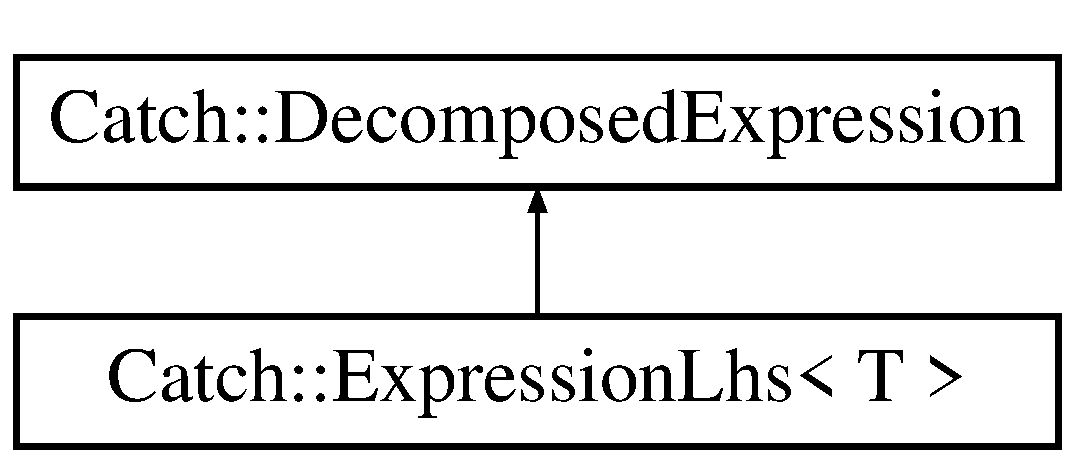
\includegraphics[height=2.000000cm]{classCatch_1_1ExpressionLhs}
\end{center}
\end{figure}
\subsection*{Public Member Functions}
\begin{DoxyCompactItemize}
\item 
\hyperlink{classCatch_1_1ExpressionLhs_aa829588def6146a94fb75de9c4cc482a}{Expression\-Lhs} (\hyperlink{classCatch_1_1ResultBuilder}{Result\-Builder} \&rb, T lhs)
\item 
\hyperlink{classCatch_1_1ExpressionLhs}{Expression\-Lhs} \& \hyperlink{classCatch_1_1ExpressionLhs_a60d50fe8adcaabcb7c93747ddbae5993}{operator=} (const \hyperlink{classCatch_1_1ExpressionLhs}{Expression\-Lhs} \&)
\item 
{\footnotesize template$<$typename Rhs\-T $>$ }\\\hyperlink{classCatch_1_1BinaryExpression}{Binary\-Expression}$<$ T, \\*
\hyperlink{namespaceCatch_1_1Internal_ae3f96598a7858155750bf38e7295d83ea30e0accba6ec8384f4383b04dd2a6a9e}{Internal\-::\-Is\-Equal\-To}, Rhs\-T \\*
const \& $>$ \hyperlink{classCatch_1_1ExpressionLhs_abebe4afc079c91ae548ab8fdba6c77f2}{operator==} (Rhs\-T const \&rhs)
\item 
{\footnotesize template$<$typename Rhs\-T $>$ }\\\hyperlink{classCatch_1_1BinaryExpression}{Binary\-Expression}$<$ T, \\*
\hyperlink{namespaceCatch_1_1Internal_ae3f96598a7858155750bf38e7295d83ea1e1699cf7d3dbee0908f1a123da2456d}{Internal\-::\-Is\-Not\-Equal\-To}, Rhs\-T \\*
const \& $>$ \hyperlink{classCatch_1_1ExpressionLhs_a3bc08bb2b9c27678e2628faa73645144}{operator!=} (Rhs\-T const \&rhs)
\item 
{\footnotesize template$<$typename Rhs\-T $>$ }\\\hyperlink{classCatch_1_1BinaryExpression}{Binary\-Expression}$<$ T, \\*
\hyperlink{namespaceCatch_1_1Internal_ae3f96598a7858155750bf38e7295d83eabbbfc41706595e50acbefa8408004b93}{Internal\-::\-Is\-Less\-Than}, Rhs\-T \\*
const \& $>$ \hyperlink{classCatch_1_1ExpressionLhs_a919c48e52ff1be5f7329920d4da8e92f}{operator$<$} (Rhs\-T const \&rhs)
\item 
{\footnotesize template$<$typename Rhs\-T $>$ }\\\hyperlink{classCatch_1_1BinaryExpression}{Binary\-Expression}$<$ T, \\*
\hyperlink{namespaceCatch_1_1Internal_ae3f96598a7858155750bf38e7295d83eac0e8866139e99803d169595af70f6c22}{Internal\-::\-Is\-Greater\-Than}, Rhs\-T \\*
const \& $>$ \hyperlink{classCatch_1_1ExpressionLhs_a52981d92ec6aad872660ae7df1abb33a}{operator$>$} (Rhs\-T const \&rhs)
\item 
{\footnotesize template$<$typename Rhs\-T $>$ }\\\hyperlink{classCatch_1_1BinaryExpression}{Binary\-Expression}$<$ T, \\*
\hyperlink{namespaceCatch_1_1Internal_ae3f96598a7858155750bf38e7295d83ea0db29a4c3f1e81260036c5e27a8407fd}{Internal\-::\-Is\-Less\-Than\-Or\-Equal\-To}, \\*
Rhs\-T const \& $>$ \hyperlink{classCatch_1_1ExpressionLhs_a1d10974a581c67cc400cd6cdd36b0000}{operator$<$=} (Rhs\-T const \&rhs)
\item 
{\footnotesize template$<$typename Rhs\-T $>$ }\\\hyperlink{classCatch_1_1BinaryExpression}{Binary\-Expression}$<$ T, \\*
\hyperlink{namespaceCatch_1_1Internal_ae3f96598a7858155750bf38e7295d83ead2de7e9565e59e36c0987e402203ce1c}{Internal\-::\-Is\-Greater\-Than\-Or\-Equal\-To}, \\*
Rhs\-T const \& $>$ \hyperlink{classCatch_1_1ExpressionLhs_a3387a494cb6b699a6c0162c79f7f533c}{operator$>$=} (Rhs\-T const \&rhs)
\item 
\hyperlink{classCatch_1_1BinaryExpression}{Binary\-Expression}$<$ T, \\*
\hyperlink{namespaceCatch_1_1Internal_ae3f96598a7858155750bf38e7295d83ea30e0accba6ec8384f4383b04dd2a6a9e}{Internal\-::\-Is\-Equal\-To}, bool $>$ \hyperlink{classCatch_1_1ExpressionLhs_ab803185079504a65b0af95f7c9669351}{operator==} (bool rhs)
\item 
\hyperlink{classCatch_1_1BinaryExpression}{Binary\-Expression}$<$ T, \\*
\hyperlink{namespaceCatch_1_1Internal_ae3f96598a7858155750bf38e7295d83ea1e1699cf7d3dbee0908f1a123da2456d}{Internal\-::\-Is\-Not\-Equal\-To}, bool $>$ \hyperlink{classCatch_1_1ExpressionLhs_a1f3ff934880623f12a4cbd9725397ccf}{operator!=} (bool rhs)
\item 
void \hyperlink{classCatch_1_1ExpressionLhs_a13d2551a927790284fb5ddf1ee2c9079}{end\-Expression} ()
\item 
virtual void \hyperlink{classCatch_1_1ExpressionLhs_a7684a053e8e88a4be475a536252630da}{reconstruct\-Expression} (std\-::string \&dest) const \hyperlink{catch_8hpp_a8ecdce4d3f57835f707915ae831eb847}{C\-A\-T\-C\-H\-\_\-\-O\-V\-E\-R\-R\-I\-D\-E}
\end{DoxyCompactItemize}


\subsection{Constructor \& Destructor Documentation}
\hypertarget{classCatch_1_1ExpressionLhs_aa829588def6146a94fb75de9c4cc482a}{\index{Catch\-::\-Expression\-Lhs@{Catch\-::\-Expression\-Lhs}!Expression\-Lhs@{Expression\-Lhs}}
\index{Expression\-Lhs@{Expression\-Lhs}!Catch::ExpressionLhs@{Catch\-::\-Expression\-Lhs}}
\subsubsection[{Expression\-Lhs}]{\setlength{\rightskip}{0pt plus 5cm}template$<$typename T$>$ {\bf Catch\-::\-Expression\-Lhs}$<$ T $>$\-::{\bf Expression\-Lhs} (
\begin{DoxyParamCaption}
\item[{{\bf Result\-Builder} \&}]{rb, }
\item[{T}]{lhs}
\end{DoxyParamCaption}
)\hspace{0.3cm}{\ttfamily [inline]}}}\label{classCatch_1_1ExpressionLhs_aa829588def6146a94fb75de9c4cc482a}


\subsection{Member Function Documentation}
\hypertarget{classCatch_1_1ExpressionLhs_a13d2551a927790284fb5ddf1ee2c9079}{\index{Catch\-::\-Expression\-Lhs@{Catch\-::\-Expression\-Lhs}!end\-Expression@{end\-Expression}}
\index{end\-Expression@{end\-Expression}!Catch::ExpressionLhs@{Catch\-::\-Expression\-Lhs}}
\subsubsection[{end\-Expression}]{\setlength{\rightskip}{0pt plus 5cm}template$<$typename T$>$ void {\bf Catch\-::\-Expression\-Lhs}$<$ T $>$\-::end\-Expression (
\begin{DoxyParamCaption}
{}
\end{DoxyParamCaption}
)\hspace{0.3cm}{\ttfamily [inline]}}}\label{classCatch_1_1ExpressionLhs_a13d2551a927790284fb5ddf1ee2c9079}
\hypertarget{classCatch_1_1ExpressionLhs_a3bc08bb2b9c27678e2628faa73645144}{\index{Catch\-::\-Expression\-Lhs@{Catch\-::\-Expression\-Lhs}!operator!=@{operator!=}}
\index{operator!=@{operator!=}!Catch::ExpressionLhs@{Catch\-::\-Expression\-Lhs}}
\subsubsection[{operator!=}]{\setlength{\rightskip}{0pt plus 5cm}template$<$typename T$>$ template$<$typename Rhs\-T $>$ {\bf Binary\-Expression}$<$T, {\bf Internal\-::\-Is\-Not\-Equal\-To}, Rhs\-T const\&$>$ {\bf Catch\-::\-Expression\-Lhs}$<$ T $>$\-::operator!= (
\begin{DoxyParamCaption}
\item[{Rhs\-T const \&}]{rhs}
\end{DoxyParamCaption}
)\hspace{0.3cm}{\ttfamily [inline]}}}\label{classCatch_1_1ExpressionLhs_a3bc08bb2b9c27678e2628faa73645144}
\hypertarget{classCatch_1_1ExpressionLhs_a1f3ff934880623f12a4cbd9725397ccf}{\index{Catch\-::\-Expression\-Lhs@{Catch\-::\-Expression\-Lhs}!operator!=@{operator!=}}
\index{operator!=@{operator!=}!Catch::ExpressionLhs@{Catch\-::\-Expression\-Lhs}}
\subsubsection[{operator!=}]{\setlength{\rightskip}{0pt plus 5cm}template$<$typename T$>$ {\bf Binary\-Expression}$<$T, {\bf Internal\-::\-Is\-Not\-Equal\-To}, bool$>$ {\bf Catch\-::\-Expression\-Lhs}$<$ T $>$\-::operator!= (
\begin{DoxyParamCaption}
\item[{bool}]{rhs}
\end{DoxyParamCaption}
)\hspace{0.3cm}{\ttfamily [inline]}}}\label{classCatch_1_1ExpressionLhs_a1f3ff934880623f12a4cbd9725397ccf}
\hypertarget{classCatch_1_1ExpressionLhs_a919c48e52ff1be5f7329920d4da8e92f}{\index{Catch\-::\-Expression\-Lhs@{Catch\-::\-Expression\-Lhs}!operator$<$@{operator$<$}}
\index{operator$<$@{operator$<$}!Catch::ExpressionLhs@{Catch\-::\-Expression\-Lhs}}
\subsubsection[{operator$<$}]{\setlength{\rightskip}{0pt plus 5cm}template$<$typename T$>$ template$<$typename Rhs\-T $>$ {\bf Binary\-Expression}$<$T, {\bf Internal\-::\-Is\-Less\-Than}, Rhs\-T const\&$>$ {\bf Catch\-::\-Expression\-Lhs}$<$ T $>$\-::operator$<$ (
\begin{DoxyParamCaption}
\item[{Rhs\-T const \&}]{rhs}
\end{DoxyParamCaption}
)\hspace{0.3cm}{\ttfamily [inline]}}}\label{classCatch_1_1ExpressionLhs_a919c48e52ff1be5f7329920d4da8e92f}
\hypertarget{classCatch_1_1ExpressionLhs_a1d10974a581c67cc400cd6cdd36b0000}{\index{Catch\-::\-Expression\-Lhs@{Catch\-::\-Expression\-Lhs}!operator$<$=@{operator$<$=}}
\index{operator$<$=@{operator$<$=}!Catch::ExpressionLhs@{Catch\-::\-Expression\-Lhs}}
\subsubsection[{operator$<$=}]{\setlength{\rightskip}{0pt plus 5cm}template$<$typename T$>$ template$<$typename Rhs\-T $>$ {\bf Binary\-Expression}$<$T, {\bf Internal\-::\-Is\-Less\-Than\-Or\-Equal\-To}, Rhs\-T const\&$>$ {\bf Catch\-::\-Expression\-Lhs}$<$ T $>$\-::operator$<$= (
\begin{DoxyParamCaption}
\item[{Rhs\-T const \&}]{rhs}
\end{DoxyParamCaption}
)\hspace{0.3cm}{\ttfamily [inline]}}}\label{classCatch_1_1ExpressionLhs_a1d10974a581c67cc400cd6cdd36b0000}
\hypertarget{classCatch_1_1ExpressionLhs_a60d50fe8adcaabcb7c93747ddbae5993}{\index{Catch\-::\-Expression\-Lhs@{Catch\-::\-Expression\-Lhs}!operator=@{operator=}}
\index{operator=@{operator=}!Catch::ExpressionLhs@{Catch\-::\-Expression\-Lhs}}
\subsubsection[{operator=}]{\setlength{\rightskip}{0pt plus 5cm}template$<$typename T$>$ {\bf Expression\-Lhs}\& {\bf Catch\-::\-Expression\-Lhs}$<$ T $>$\-::operator= (
\begin{DoxyParamCaption}
\item[{const {\bf Expression\-Lhs}$<$ T $>$ \&}]{}
\end{DoxyParamCaption}
)}}\label{classCatch_1_1ExpressionLhs_a60d50fe8adcaabcb7c93747ddbae5993}
\hypertarget{classCatch_1_1ExpressionLhs_abebe4afc079c91ae548ab8fdba6c77f2}{\index{Catch\-::\-Expression\-Lhs@{Catch\-::\-Expression\-Lhs}!operator==@{operator==}}
\index{operator==@{operator==}!Catch::ExpressionLhs@{Catch\-::\-Expression\-Lhs}}
\subsubsection[{operator==}]{\setlength{\rightskip}{0pt plus 5cm}template$<$typename T$>$ template$<$typename Rhs\-T $>$ {\bf Binary\-Expression}$<$T, {\bf Internal\-::\-Is\-Equal\-To}, Rhs\-T const\&$>$ {\bf Catch\-::\-Expression\-Lhs}$<$ T $>$\-::operator== (
\begin{DoxyParamCaption}
\item[{Rhs\-T const \&}]{rhs}
\end{DoxyParamCaption}
)\hspace{0.3cm}{\ttfamily [inline]}}}\label{classCatch_1_1ExpressionLhs_abebe4afc079c91ae548ab8fdba6c77f2}
\hypertarget{classCatch_1_1ExpressionLhs_ab803185079504a65b0af95f7c9669351}{\index{Catch\-::\-Expression\-Lhs@{Catch\-::\-Expression\-Lhs}!operator==@{operator==}}
\index{operator==@{operator==}!Catch::ExpressionLhs@{Catch\-::\-Expression\-Lhs}}
\subsubsection[{operator==}]{\setlength{\rightskip}{0pt plus 5cm}template$<$typename T$>$ {\bf Binary\-Expression}$<$T, {\bf Internal\-::\-Is\-Equal\-To}, bool$>$ {\bf Catch\-::\-Expression\-Lhs}$<$ T $>$\-::operator== (
\begin{DoxyParamCaption}
\item[{bool}]{rhs}
\end{DoxyParamCaption}
)\hspace{0.3cm}{\ttfamily [inline]}}}\label{classCatch_1_1ExpressionLhs_ab803185079504a65b0af95f7c9669351}
\hypertarget{classCatch_1_1ExpressionLhs_a52981d92ec6aad872660ae7df1abb33a}{\index{Catch\-::\-Expression\-Lhs@{Catch\-::\-Expression\-Lhs}!operator$>$@{operator$>$}}
\index{operator$>$@{operator$>$}!Catch::ExpressionLhs@{Catch\-::\-Expression\-Lhs}}
\subsubsection[{operator$>$}]{\setlength{\rightskip}{0pt plus 5cm}template$<$typename T$>$ template$<$typename Rhs\-T $>$ {\bf Binary\-Expression}$<$T, {\bf Internal\-::\-Is\-Greater\-Than}, Rhs\-T const\&$>$ {\bf Catch\-::\-Expression\-Lhs}$<$ T $>$\-::operator$>$ (
\begin{DoxyParamCaption}
\item[{Rhs\-T const \&}]{rhs}
\end{DoxyParamCaption}
)\hspace{0.3cm}{\ttfamily [inline]}}}\label{classCatch_1_1ExpressionLhs_a52981d92ec6aad872660ae7df1abb33a}
\hypertarget{classCatch_1_1ExpressionLhs_a3387a494cb6b699a6c0162c79f7f533c}{\index{Catch\-::\-Expression\-Lhs@{Catch\-::\-Expression\-Lhs}!operator$>$=@{operator$>$=}}
\index{operator$>$=@{operator$>$=}!Catch::ExpressionLhs@{Catch\-::\-Expression\-Lhs}}
\subsubsection[{operator$>$=}]{\setlength{\rightskip}{0pt plus 5cm}template$<$typename T$>$ template$<$typename Rhs\-T $>$ {\bf Binary\-Expression}$<$T, {\bf Internal\-::\-Is\-Greater\-Than\-Or\-Equal\-To}, Rhs\-T const\&$>$ {\bf Catch\-::\-Expression\-Lhs}$<$ T $>$\-::operator$>$= (
\begin{DoxyParamCaption}
\item[{Rhs\-T const \&}]{rhs}
\end{DoxyParamCaption}
)\hspace{0.3cm}{\ttfamily [inline]}}}\label{classCatch_1_1ExpressionLhs_a3387a494cb6b699a6c0162c79f7f533c}
\hypertarget{classCatch_1_1ExpressionLhs_a7684a053e8e88a4be475a536252630da}{\index{Catch\-::\-Expression\-Lhs@{Catch\-::\-Expression\-Lhs}!reconstruct\-Expression@{reconstruct\-Expression}}
\index{reconstruct\-Expression@{reconstruct\-Expression}!Catch::ExpressionLhs@{Catch\-::\-Expression\-Lhs}}
\subsubsection[{reconstruct\-Expression}]{\setlength{\rightskip}{0pt plus 5cm}template$<$typename T$>$ virtual void {\bf Catch\-::\-Expression\-Lhs}$<$ T $>$\-::reconstruct\-Expression (
\begin{DoxyParamCaption}
\item[{std\-::string \&}]{dest}
\end{DoxyParamCaption}
) const\hspace{0.3cm}{\ttfamily [inline]}, {\ttfamily [virtual]}}}\label{classCatch_1_1ExpressionLhs_a7684a053e8e88a4be475a536252630da}


Implements \hyperlink{structCatch_1_1DecomposedExpression_a9ce7f356dc96f11f80e40c82f5aa7e55}{Catch\-::\-Decomposed\-Expression}.



The documentation for this class was generated from the following file\-:\begin{DoxyCompactItemize}
\item 
/home/alexander/\-Un\-B/\-M\-P/\-Trabalho\-\_\-2\-\_\-\-M\-P\-\_\-\-Alexander\-\_\-13\-\_\-0039853/include/\hyperlink{catch_8hpp}{catch.\-hpp}\end{DoxyCompactItemize}

\hypertarget{structCatch_1_1Detail_1_1FalseType}{\section{Catch\-:\-:Detail\-:\-:False\-Type Struct Reference}
\label{structCatch_1_1Detail_1_1FalseType}\index{Catch\-::\-Detail\-::\-False\-Type@{Catch\-::\-Detail\-::\-False\-Type}}
}


{\ttfamily \#include $<$catch.\-hpp$>$}

\subsection*{Public Attributes}
\begin{DoxyCompactItemize}
\item 
char \hyperlink{structCatch_1_1Detail_1_1FalseType_abc1a730e197d6f7750ae8aaf47b63477}{sizer} \mbox{[}2\mbox{]}
\end{DoxyCompactItemize}


\subsection{Member Data Documentation}
\hypertarget{structCatch_1_1Detail_1_1FalseType_abc1a730e197d6f7750ae8aaf47b63477}{\index{Catch\-::\-Detail\-::\-False\-Type@{Catch\-::\-Detail\-::\-False\-Type}!sizer@{sizer}}
\index{sizer@{sizer}!Catch::Detail::FalseType@{Catch\-::\-Detail\-::\-False\-Type}}
\subsubsection[{sizer}]{\setlength{\rightskip}{0pt plus 5cm}char Catch\-::\-Detail\-::\-False\-Type\-::sizer\mbox{[}2\mbox{]}}}\label{structCatch_1_1Detail_1_1FalseType_abc1a730e197d6f7750ae8aaf47b63477}


The documentation for this struct was generated from the following file\-:\begin{DoxyCompactItemize}
\item 
/home/alexander/\-Un\-B/\-M\-P/\-Trabalho\-\_\-2\-\_\-\-M\-P\-\_\-\-Alexander\-\_\-13\-\_\-0039853/include/\hyperlink{catch_8hpp}{catch.\-hpp}\end{DoxyCompactItemize}

\hypertarget{structCatch_1_1IContext}{\section{Catch\-:\-:I\-Context Struct Reference}
\label{structCatch_1_1IContext}\index{Catch\-::\-I\-Context@{Catch\-::\-I\-Context}}
}


{\ttfamily \#include $<$catch.\-hpp$>$}

Inheritance diagram for Catch\-:\-:I\-Context\-:\begin{figure}[H]
\begin{center}
\leavevmode
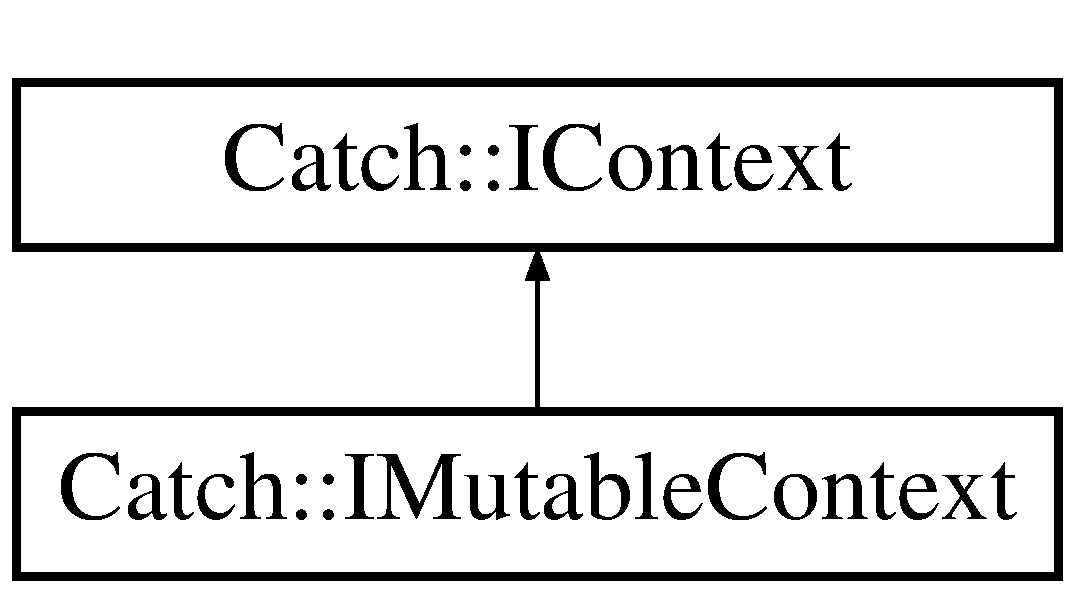
\includegraphics[height=2.000000cm]{structCatch_1_1IContext}
\end{center}
\end{figure}
\subsection*{Public Member Functions}
\begin{DoxyCompactItemize}
\item 
virtual \hyperlink{structCatch_1_1IContext_aeb17355c1be6c2ced5407cad7202628d}{$\sim$\-I\-Context} ()
\item 
virtual \hyperlink{structCatch_1_1IResultCapture}{I\-Result\-Capture} $\ast$ \hyperlink{structCatch_1_1IContext_a684e4ae71d1fdf3060c352ecde1d122f}{get\-Result\-Capture} ()=0
\item 
virtual \hyperlink{structCatch_1_1IRunner}{I\-Runner} $\ast$ \hyperlink{structCatch_1_1IContext_af088415dde18d039ed5a2f95b02767c6}{get\-Runner} ()=0
\item 
virtual size\-\_\-t \hyperlink{structCatch_1_1IContext_a43e07088db43299ba129fbe6d3106e95}{get\-Generator\-Index} (std\-::string const \&file\-Info, size\-\_\-t total\-Size)=0
\item 
virtual bool \hyperlink{structCatch_1_1IContext_a806f7c4ed24d51adae90418e661b24b7}{advance\-Generators\-For\-Current\-Test} ()=0
\item 
virtual \hyperlink{classCatch_1_1Ptr}{Ptr}$<$ I\-Config const  $>$ \hyperlink{structCatch_1_1IContext_aee81c415899262e096ad8d6f686fa365}{get\-Config} () const =0
\end{DoxyCompactItemize}


\subsection{Constructor \& Destructor Documentation}
\hypertarget{structCatch_1_1IContext_aeb17355c1be6c2ced5407cad7202628d}{\index{Catch\-::\-I\-Context@{Catch\-::\-I\-Context}!$\sim$\-I\-Context@{$\sim$\-I\-Context}}
\index{$\sim$\-I\-Context@{$\sim$\-I\-Context}!Catch::IContext@{Catch\-::\-I\-Context}}
\subsubsection[{$\sim$\-I\-Context}]{\setlength{\rightskip}{0pt plus 5cm}virtual Catch\-::\-I\-Context\-::$\sim$\-I\-Context (
\begin{DoxyParamCaption}
{}
\end{DoxyParamCaption}
)\hspace{0.3cm}{\ttfamily [virtual]}}}\label{structCatch_1_1IContext_aeb17355c1be6c2ced5407cad7202628d}


\subsection{Member Function Documentation}
\hypertarget{structCatch_1_1IContext_a806f7c4ed24d51adae90418e661b24b7}{\index{Catch\-::\-I\-Context@{Catch\-::\-I\-Context}!advance\-Generators\-For\-Current\-Test@{advance\-Generators\-For\-Current\-Test}}
\index{advance\-Generators\-For\-Current\-Test@{advance\-Generators\-For\-Current\-Test}!Catch::IContext@{Catch\-::\-I\-Context}}
\subsubsection[{advance\-Generators\-For\-Current\-Test}]{\setlength{\rightskip}{0pt plus 5cm}virtual bool Catch\-::\-I\-Context\-::advance\-Generators\-For\-Current\-Test (
\begin{DoxyParamCaption}
{}
\end{DoxyParamCaption}
)\hspace{0.3cm}{\ttfamily [pure virtual]}}}\label{structCatch_1_1IContext_a806f7c4ed24d51adae90418e661b24b7}
\hypertarget{structCatch_1_1IContext_aee81c415899262e096ad8d6f686fa365}{\index{Catch\-::\-I\-Context@{Catch\-::\-I\-Context}!get\-Config@{get\-Config}}
\index{get\-Config@{get\-Config}!Catch::IContext@{Catch\-::\-I\-Context}}
\subsubsection[{get\-Config}]{\setlength{\rightskip}{0pt plus 5cm}virtual {\bf Ptr}$<$I\-Config const$>$ Catch\-::\-I\-Context\-::get\-Config (
\begin{DoxyParamCaption}
{}
\end{DoxyParamCaption}
) const\hspace{0.3cm}{\ttfamily [pure virtual]}}}\label{structCatch_1_1IContext_aee81c415899262e096ad8d6f686fa365}
\hypertarget{structCatch_1_1IContext_a43e07088db43299ba129fbe6d3106e95}{\index{Catch\-::\-I\-Context@{Catch\-::\-I\-Context}!get\-Generator\-Index@{get\-Generator\-Index}}
\index{get\-Generator\-Index@{get\-Generator\-Index}!Catch::IContext@{Catch\-::\-I\-Context}}
\subsubsection[{get\-Generator\-Index}]{\setlength{\rightskip}{0pt plus 5cm}virtual size\-\_\-t Catch\-::\-I\-Context\-::get\-Generator\-Index (
\begin{DoxyParamCaption}
\item[{std\-::string const \&}]{file\-Info, }
\item[{size\-\_\-t}]{total\-Size}
\end{DoxyParamCaption}
)\hspace{0.3cm}{\ttfamily [pure virtual]}}}\label{structCatch_1_1IContext_a43e07088db43299ba129fbe6d3106e95}
\hypertarget{structCatch_1_1IContext_a684e4ae71d1fdf3060c352ecde1d122f}{\index{Catch\-::\-I\-Context@{Catch\-::\-I\-Context}!get\-Result\-Capture@{get\-Result\-Capture}}
\index{get\-Result\-Capture@{get\-Result\-Capture}!Catch::IContext@{Catch\-::\-I\-Context}}
\subsubsection[{get\-Result\-Capture}]{\setlength{\rightskip}{0pt plus 5cm}virtual {\bf I\-Result\-Capture}$\ast$ Catch\-::\-I\-Context\-::get\-Result\-Capture (
\begin{DoxyParamCaption}
{}
\end{DoxyParamCaption}
)\hspace{0.3cm}{\ttfamily [pure virtual]}}}\label{structCatch_1_1IContext_a684e4ae71d1fdf3060c352ecde1d122f}
\hypertarget{structCatch_1_1IContext_af088415dde18d039ed5a2f95b02767c6}{\index{Catch\-::\-I\-Context@{Catch\-::\-I\-Context}!get\-Runner@{get\-Runner}}
\index{get\-Runner@{get\-Runner}!Catch::IContext@{Catch\-::\-I\-Context}}
\subsubsection[{get\-Runner}]{\setlength{\rightskip}{0pt plus 5cm}virtual {\bf I\-Runner}$\ast$ Catch\-::\-I\-Context\-::get\-Runner (
\begin{DoxyParamCaption}
{}
\end{DoxyParamCaption}
)\hspace{0.3cm}{\ttfamily [pure virtual]}}}\label{structCatch_1_1IContext_af088415dde18d039ed5a2f95b02767c6}


The documentation for this struct was generated from the following file\-:\begin{DoxyCompactItemize}
\item 
/home/alexander/\-Un\-B/\-M\-P/\-Trabalho\-\_\-2\-\_\-\-M\-P\-\_\-\-Alexander\-\_\-13\-\_\-0039853/include/\hyperlink{catch_8hpp}{catch.\-hpp}\end{DoxyCompactItemize}

\hypertarget{structCatch_1_1IExceptionTranslator}{\section{Catch\-:\-:I\-Exception\-Translator Struct Reference}
\label{structCatch_1_1IExceptionTranslator}\index{Catch\-::\-I\-Exception\-Translator@{Catch\-::\-I\-Exception\-Translator}}
}


{\ttfamily \#include $<$catch.\-hpp$>$}

\subsection*{Public Member Functions}
\begin{DoxyCompactItemize}
\item 
virtual \hyperlink{structCatch_1_1IExceptionTranslator_afa00bb6258c07591df472aadae05783f}{$\sim$\-I\-Exception\-Translator} ()
\item 
virtual std\-::string \hyperlink{structCatch_1_1IExceptionTranslator_a2a554b96ed5ed411e7c796b6b42837a5}{translate} (Exception\-Translators\-::const\-\_\-iterator it, Exception\-Translators\-::const\-\_\-iterator it\-End) const =0
\end{DoxyCompactItemize}


\subsection{Constructor \& Destructor Documentation}
\hypertarget{structCatch_1_1IExceptionTranslator_afa00bb6258c07591df472aadae05783f}{\index{Catch\-::\-I\-Exception\-Translator@{Catch\-::\-I\-Exception\-Translator}!$\sim$\-I\-Exception\-Translator@{$\sim$\-I\-Exception\-Translator}}
\index{$\sim$\-I\-Exception\-Translator@{$\sim$\-I\-Exception\-Translator}!Catch::IExceptionTranslator@{Catch\-::\-I\-Exception\-Translator}}
\subsubsection[{$\sim$\-I\-Exception\-Translator}]{\setlength{\rightskip}{0pt plus 5cm}virtual Catch\-::\-I\-Exception\-Translator\-::$\sim$\-I\-Exception\-Translator (
\begin{DoxyParamCaption}
{}
\end{DoxyParamCaption}
)\hspace{0.3cm}{\ttfamily [virtual]}}}\label{structCatch_1_1IExceptionTranslator_afa00bb6258c07591df472aadae05783f}


\subsection{Member Function Documentation}
\hypertarget{structCatch_1_1IExceptionTranslator_a2a554b96ed5ed411e7c796b6b42837a5}{\index{Catch\-::\-I\-Exception\-Translator@{Catch\-::\-I\-Exception\-Translator}!translate@{translate}}
\index{translate@{translate}!Catch::IExceptionTranslator@{Catch\-::\-I\-Exception\-Translator}}
\subsubsection[{translate}]{\setlength{\rightskip}{0pt plus 5cm}virtual std\-::string Catch\-::\-I\-Exception\-Translator\-::translate (
\begin{DoxyParamCaption}
\item[{Exception\-Translators\-::const\-\_\-iterator}]{it, }
\item[{Exception\-Translators\-::const\-\_\-iterator}]{it\-End}
\end{DoxyParamCaption}
) const\hspace{0.3cm}{\ttfamily [pure virtual]}}}\label{structCatch_1_1IExceptionTranslator_a2a554b96ed5ed411e7c796b6b42837a5}


The documentation for this struct was generated from the following file\-:\begin{DoxyCompactItemize}
\item 
/home/alexander/\-Un\-B/\-M\-P/\-Trabalho\-\_\-2\-\_\-\-M\-P\-\_\-\-Alexander\-\_\-13\-\_\-0039853/include/\hyperlink{catch_8hpp}{catch.\-hpp}\end{DoxyCompactItemize}

\hypertarget{structCatch_1_1IExceptionTranslatorRegistry}{\section{Catch\-:\-:I\-Exception\-Translator\-Registry Struct Reference}
\label{structCatch_1_1IExceptionTranslatorRegistry}\index{Catch\-::\-I\-Exception\-Translator\-Registry@{Catch\-::\-I\-Exception\-Translator\-Registry}}
}


{\ttfamily \#include $<$catch.\-hpp$>$}

\subsection*{Public Member Functions}
\begin{DoxyCompactItemize}
\item 
virtual \hyperlink{structCatch_1_1IExceptionTranslatorRegistry_acf7402e18789ea46d54ea8564ac358d3}{$\sim$\-I\-Exception\-Translator\-Registry} ()
\item 
virtual std\-::string \hyperlink{structCatch_1_1IExceptionTranslatorRegistry_af76ae8c331a17f2a94c9720bc0d686bb}{translate\-Active\-Exception} () const =0
\end{DoxyCompactItemize}


\subsection{Constructor \& Destructor Documentation}
\hypertarget{structCatch_1_1IExceptionTranslatorRegistry_acf7402e18789ea46d54ea8564ac358d3}{\index{Catch\-::\-I\-Exception\-Translator\-Registry@{Catch\-::\-I\-Exception\-Translator\-Registry}!$\sim$\-I\-Exception\-Translator\-Registry@{$\sim$\-I\-Exception\-Translator\-Registry}}
\index{$\sim$\-I\-Exception\-Translator\-Registry@{$\sim$\-I\-Exception\-Translator\-Registry}!Catch::IExceptionTranslatorRegistry@{Catch\-::\-I\-Exception\-Translator\-Registry}}
\subsubsection[{$\sim$\-I\-Exception\-Translator\-Registry}]{\setlength{\rightskip}{0pt plus 5cm}virtual Catch\-::\-I\-Exception\-Translator\-Registry\-::$\sim$\-I\-Exception\-Translator\-Registry (
\begin{DoxyParamCaption}
{}
\end{DoxyParamCaption}
)\hspace{0.3cm}{\ttfamily [virtual]}}}\label{structCatch_1_1IExceptionTranslatorRegistry_acf7402e18789ea46d54ea8564ac358d3}


\subsection{Member Function Documentation}
\hypertarget{structCatch_1_1IExceptionTranslatorRegistry_af76ae8c331a17f2a94c9720bc0d686bb}{\index{Catch\-::\-I\-Exception\-Translator\-Registry@{Catch\-::\-I\-Exception\-Translator\-Registry}!translate\-Active\-Exception@{translate\-Active\-Exception}}
\index{translate\-Active\-Exception@{translate\-Active\-Exception}!Catch::IExceptionTranslatorRegistry@{Catch\-::\-I\-Exception\-Translator\-Registry}}
\subsubsection[{translate\-Active\-Exception}]{\setlength{\rightskip}{0pt plus 5cm}virtual std\-::string Catch\-::\-I\-Exception\-Translator\-Registry\-::translate\-Active\-Exception (
\begin{DoxyParamCaption}
{}
\end{DoxyParamCaption}
) const\hspace{0.3cm}{\ttfamily [pure virtual]}}}\label{structCatch_1_1IExceptionTranslatorRegistry_af76ae8c331a17f2a94c9720bc0d686bb}


The documentation for this struct was generated from the following file\-:\begin{DoxyCompactItemize}
\item 
/home/alexander/\-Un\-B/\-M\-P/\-Trabalho\-\_\-2\-\_\-\-M\-P\-\_\-\-Alexander\-\_\-13\-\_\-0039853/include/\hyperlink{catch_8hpp}{catch.\-hpp}\end{DoxyCompactItemize}

\hypertarget{structCatch_1_1IGenerator}{\section{Catch\-:\-:I\-Generator$<$ T $>$ Struct Template Reference}
\label{structCatch_1_1IGenerator}\index{Catch\-::\-I\-Generator$<$ T $>$@{Catch\-::\-I\-Generator$<$ T $>$}}
}


{\ttfamily \#include $<$catch.\-hpp$>$}

Inheritance diagram for Catch\-:\-:I\-Generator$<$ T $>$\-:\begin{figure}[H]
\begin{center}
\leavevmode
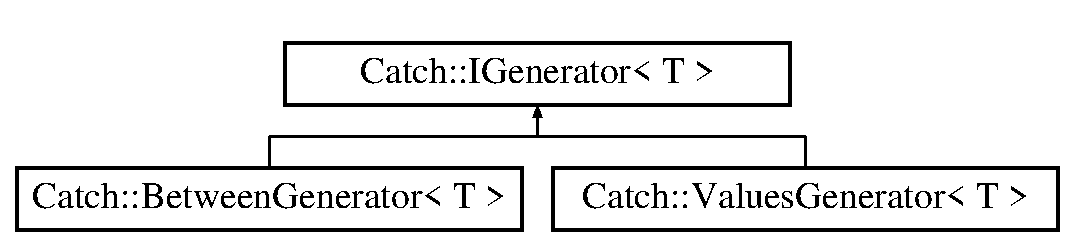
\includegraphics[height=2.000000cm]{structCatch_1_1IGenerator}
\end{center}
\end{figure}
\subsection*{Public Member Functions}
\begin{DoxyCompactItemize}
\item 
virtual \hyperlink{structCatch_1_1IGenerator_a0622037f4617e09aa8c584b0144d4a1a}{$\sim$\-I\-Generator} ()
\item 
virtual T \hyperlink{structCatch_1_1IGenerator_ad69e937cb66dba3ed9429c42abf4fce3}{get\-Value} (std\-::size\-\_\-t index) const =0
\item 
virtual std\-::size\-\_\-t \hyperlink{structCatch_1_1IGenerator_a2e317253b03e838b6065ce69719a198e}{size} () const =0
\end{DoxyCompactItemize}


\subsection{Constructor \& Destructor Documentation}
\hypertarget{structCatch_1_1IGenerator_a0622037f4617e09aa8c584b0144d4a1a}{\index{Catch\-::\-I\-Generator@{Catch\-::\-I\-Generator}!$\sim$\-I\-Generator@{$\sim$\-I\-Generator}}
\index{$\sim$\-I\-Generator@{$\sim$\-I\-Generator}!Catch::IGenerator@{Catch\-::\-I\-Generator}}
\subsubsection[{$\sim$\-I\-Generator}]{\setlength{\rightskip}{0pt plus 5cm}template$<$typename T$>$ virtual {\bf Catch\-::\-I\-Generator}$<$ T $>$\-::$\sim${\bf I\-Generator} (
\begin{DoxyParamCaption}
{}
\end{DoxyParamCaption}
)\hspace{0.3cm}{\ttfamily [inline]}, {\ttfamily [virtual]}}}\label{structCatch_1_1IGenerator_a0622037f4617e09aa8c584b0144d4a1a}


\subsection{Member Function Documentation}
\hypertarget{structCatch_1_1IGenerator_ad69e937cb66dba3ed9429c42abf4fce3}{\index{Catch\-::\-I\-Generator@{Catch\-::\-I\-Generator}!get\-Value@{get\-Value}}
\index{get\-Value@{get\-Value}!Catch::IGenerator@{Catch\-::\-I\-Generator}}
\subsubsection[{get\-Value}]{\setlength{\rightskip}{0pt plus 5cm}template$<$typename T$>$ virtual T {\bf Catch\-::\-I\-Generator}$<$ T $>$\-::get\-Value (
\begin{DoxyParamCaption}
\item[{std\-::size\-\_\-t}]{index}
\end{DoxyParamCaption}
) const\hspace{0.3cm}{\ttfamily [pure virtual]}}}\label{structCatch_1_1IGenerator_ad69e937cb66dba3ed9429c42abf4fce3}


Implemented in \hyperlink{classCatch_1_1ValuesGenerator_a60599dd67096ff108471f64ee42acd9d}{Catch\-::\-Values\-Generator$<$ T $>$}, and \hyperlink{classCatch_1_1BetweenGenerator_af83575d62cc727ca995446cff4d6c26c}{Catch\-::\-Between\-Generator$<$ T $>$}.

\hypertarget{structCatch_1_1IGenerator_a2e317253b03e838b6065ce69719a198e}{\index{Catch\-::\-I\-Generator@{Catch\-::\-I\-Generator}!size@{size}}
\index{size@{size}!Catch::IGenerator@{Catch\-::\-I\-Generator}}
\subsubsection[{size}]{\setlength{\rightskip}{0pt plus 5cm}template$<$typename T$>$ virtual std\-::size\-\_\-t {\bf Catch\-::\-I\-Generator}$<$ T $>$\-::size (
\begin{DoxyParamCaption}
{}
\end{DoxyParamCaption}
) const\hspace{0.3cm}{\ttfamily [pure virtual]}}}\label{structCatch_1_1IGenerator_a2e317253b03e838b6065ce69719a198e}


Implemented in \hyperlink{classCatch_1_1ValuesGenerator_a98a80bb0dd682c44e82e4a75e98c4682}{Catch\-::\-Values\-Generator$<$ T $>$}, and \hyperlink{classCatch_1_1BetweenGenerator_aa53a04a259e796ba2b5adabed79474b5}{Catch\-::\-Between\-Generator$<$ T $>$}.



The documentation for this struct was generated from the following file\-:\begin{DoxyCompactItemize}
\item 
/home/alexander/\-Un\-B/\-M\-P/\-Trabalho\-\_\-2\-\_\-\-M\-P\-\_\-\-Alexander\-\_\-13\-\_\-0039853/include/\hyperlink{catch_8hpp}{catch.\-hpp}\end{DoxyCompactItemize}

\hypertarget{structCatch_1_1IGeneratorInfo}{\section{Catch\-:\-:I\-Generator\-Info Struct Reference}
\label{structCatch_1_1IGeneratorInfo}\index{Catch\-::\-I\-Generator\-Info@{Catch\-::\-I\-Generator\-Info}}
}


{\ttfamily \#include $<$catch.\-hpp$>$}

\subsection*{Public Member Functions}
\begin{DoxyCompactItemize}
\item 
virtual \hyperlink{structCatch_1_1IGeneratorInfo_a9266aa62993298510c2a8b5948abb8e6}{$\sim$\-I\-Generator\-Info} ()
\item 
virtual bool \hyperlink{structCatch_1_1IGeneratorInfo_a2b86711ca7009903edfe27ed62b515ef}{move\-Next} ()=0
\item 
virtual std\-::size\-\_\-t \hyperlink{structCatch_1_1IGeneratorInfo_a6a0dca712d31f6849fd9447b1344673a}{get\-Current\-Index} () const =0
\end{DoxyCompactItemize}


\subsection{Constructor \& Destructor Documentation}
\hypertarget{structCatch_1_1IGeneratorInfo_a9266aa62993298510c2a8b5948abb8e6}{\index{Catch\-::\-I\-Generator\-Info@{Catch\-::\-I\-Generator\-Info}!$\sim$\-I\-Generator\-Info@{$\sim$\-I\-Generator\-Info}}
\index{$\sim$\-I\-Generator\-Info@{$\sim$\-I\-Generator\-Info}!Catch::IGeneratorInfo@{Catch\-::\-I\-Generator\-Info}}
\subsubsection[{$\sim$\-I\-Generator\-Info}]{\setlength{\rightskip}{0pt plus 5cm}virtual Catch\-::\-I\-Generator\-Info\-::$\sim$\-I\-Generator\-Info (
\begin{DoxyParamCaption}
{}
\end{DoxyParamCaption}
)\hspace{0.3cm}{\ttfamily [virtual]}}}\label{structCatch_1_1IGeneratorInfo_a9266aa62993298510c2a8b5948abb8e6}


\subsection{Member Function Documentation}
\hypertarget{structCatch_1_1IGeneratorInfo_a6a0dca712d31f6849fd9447b1344673a}{\index{Catch\-::\-I\-Generator\-Info@{Catch\-::\-I\-Generator\-Info}!get\-Current\-Index@{get\-Current\-Index}}
\index{get\-Current\-Index@{get\-Current\-Index}!Catch::IGeneratorInfo@{Catch\-::\-I\-Generator\-Info}}
\subsubsection[{get\-Current\-Index}]{\setlength{\rightskip}{0pt plus 5cm}virtual std\-::size\-\_\-t Catch\-::\-I\-Generator\-Info\-::get\-Current\-Index (
\begin{DoxyParamCaption}
{}
\end{DoxyParamCaption}
) const\hspace{0.3cm}{\ttfamily [pure virtual]}}}\label{structCatch_1_1IGeneratorInfo_a6a0dca712d31f6849fd9447b1344673a}
\hypertarget{structCatch_1_1IGeneratorInfo_a2b86711ca7009903edfe27ed62b515ef}{\index{Catch\-::\-I\-Generator\-Info@{Catch\-::\-I\-Generator\-Info}!move\-Next@{move\-Next}}
\index{move\-Next@{move\-Next}!Catch::IGeneratorInfo@{Catch\-::\-I\-Generator\-Info}}
\subsubsection[{move\-Next}]{\setlength{\rightskip}{0pt plus 5cm}virtual bool Catch\-::\-I\-Generator\-Info\-::move\-Next (
\begin{DoxyParamCaption}
{}
\end{DoxyParamCaption}
)\hspace{0.3cm}{\ttfamily [pure virtual]}}}\label{structCatch_1_1IGeneratorInfo_a2b86711ca7009903edfe27ed62b515ef}


The documentation for this struct was generated from the following file\-:\begin{DoxyCompactItemize}
\item 
/home/alexander/\-Un\-B/\-M\-P/\-Trabalho\-\_\-2\-\_\-\-M\-P\-\_\-\-Alexander\-\_\-13\-\_\-0039853/include/\hyperlink{catch_8hpp}{catch.\-hpp}\end{DoxyCompactItemize}

\hypertarget{structCatch_1_1IGeneratorsForTest}{\section{Catch\-:\-:I\-Generators\-For\-Test Struct Reference}
\label{structCatch_1_1IGeneratorsForTest}\index{Catch\-::\-I\-Generators\-For\-Test@{Catch\-::\-I\-Generators\-For\-Test}}
}


{\ttfamily \#include $<$catch.\-hpp$>$}

\subsection*{Public Member Functions}
\begin{DoxyCompactItemize}
\item 
virtual \hyperlink{structCatch_1_1IGeneratorsForTest_a05725e76ee92e498f73479a61f3e3c7c}{$\sim$\-I\-Generators\-For\-Test} ()
\item 
virtual \hyperlink{structCatch_1_1IGeneratorInfo}{I\-Generator\-Info} \& \hyperlink{structCatch_1_1IGeneratorsForTest_a180d84e858840188e4c3788e47eefdb0}{get\-Generator\-Info} (std\-::string const \&file\-Info, std\-::size\-\_\-t size)=0
\item 
virtual bool \hyperlink{structCatch_1_1IGeneratorsForTest_adab31832d529fc584fd63164e0a1c8ad}{move\-Next} ()=0
\end{DoxyCompactItemize}


\subsection{Constructor \& Destructor Documentation}
\hypertarget{structCatch_1_1IGeneratorsForTest_a05725e76ee92e498f73479a61f3e3c7c}{\index{Catch\-::\-I\-Generators\-For\-Test@{Catch\-::\-I\-Generators\-For\-Test}!$\sim$\-I\-Generators\-For\-Test@{$\sim$\-I\-Generators\-For\-Test}}
\index{$\sim$\-I\-Generators\-For\-Test@{$\sim$\-I\-Generators\-For\-Test}!Catch::IGeneratorsForTest@{Catch\-::\-I\-Generators\-For\-Test}}
\subsubsection[{$\sim$\-I\-Generators\-For\-Test}]{\setlength{\rightskip}{0pt plus 5cm}virtual Catch\-::\-I\-Generators\-For\-Test\-::$\sim$\-I\-Generators\-For\-Test (
\begin{DoxyParamCaption}
{}
\end{DoxyParamCaption}
)\hspace{0.3cm}{\ttfamily [virtual]}}}\label{structCatch_1_1IGeneratorsForTest_a05725e76ee92e498f73479a61f3e3c7c}


\subsection{Member Function Documentation}
\hypertarget{structCatch_1_1IGeneratorsForTest_a180d84e858840188e4c3788e47eefdb0}{\index{Catch\-::\-I\-Generators\-For\-Test@{Catch\-::\-I\-Generators\-For\-Test}!get\-Generator\-Info@{get\-Generator\-Info}}
\index{get\-Generator\-Info@{get\-Generator\-Info}!Catch::IGeneratorsForTest@{Catch\-::\-I\-Generators\-For\-Test}}
\subsubsection[{get\-Generator\-Info}]{\setlength{\rightskip}{0pt plus 5cm}virtual {\bf I\-Generator\-Info}\& Catch\-::\-I\-Generators\-For\-Test\-::get\-Generator\-Info (
\begin{DoxyParamCaption}
\item[{std\-::string const \&}]{file\-Info, }
\item[{std\-::size\-\_\-t}]{size}
\end{DoxyParamCaption}
)\hspace{0.3cm}{\ttfamily [pure virtual]}}}\label{structCatch_1_1IGeneratorsForTest_a180d84e858840188e4c3788e47eefdb0}
\hypertarget{structCatch_1_1IGeneratorsForTest_adab31832d529fc584fd63164e0a1c8ad}{\index{Catch\-::\-I\-Generators\-For\-Test@{Catch\-::\-I\-Generators\-For\-Test}!move\-Next@{move\-Next}}
\index{move\-Next@{move\-Next}!Catch::IGeneratorsForTest@{Catch\-::\-I\-Generators\-For\-Test}}
\subsubsection[{move\-Next}]{\setlength{\rightskip}{0pt plus 5cm}virtual bool Catch\-::\-I\-Generators\-For\-Test\-::move\-Next (
\begin{DoxyParamCaption}
{}
\end{DoxyParamCaption}
)\hspace{0.3cm}{\ttfamily [pure virtual]}}}\label{structCatch_1_1IGeneratorsForTest_adab31832d529fc584fd63164e0a1c8ad}


The documentation for this struct was generated from the following file\-:\begin{DoxyCompactItemize}
\item 
/home/alexander/\-Un\-B/\-M\-P/\-Trabalho\-\_\-2\-\_\-\-M\-P\-\_\-\-Alexander\-\_\-13\-\_\-0039853/include/\hyperlink{catch_8hpp}{catch.\-hpp}\end{DoxyCompactItemize}

\hypertarget{structCatch_1_1IMutableContext}{\section{Catch\-:\-:I\-Mutable\-Context Struct Reference}
\label{structCatch_1_1IMutableContext}\index{Catch\-::\-I\-Mutable\-Context@{Catch\-::\-I\-Mutable\-Context}}
}


{\ttfamily \#include $<$catch.\-hpp$>$}

Inheritance diagram for Catch\-:\-:I\-Mutable\-Context\-:\begin{figure}[H]
\begin{center}
\leavevmode
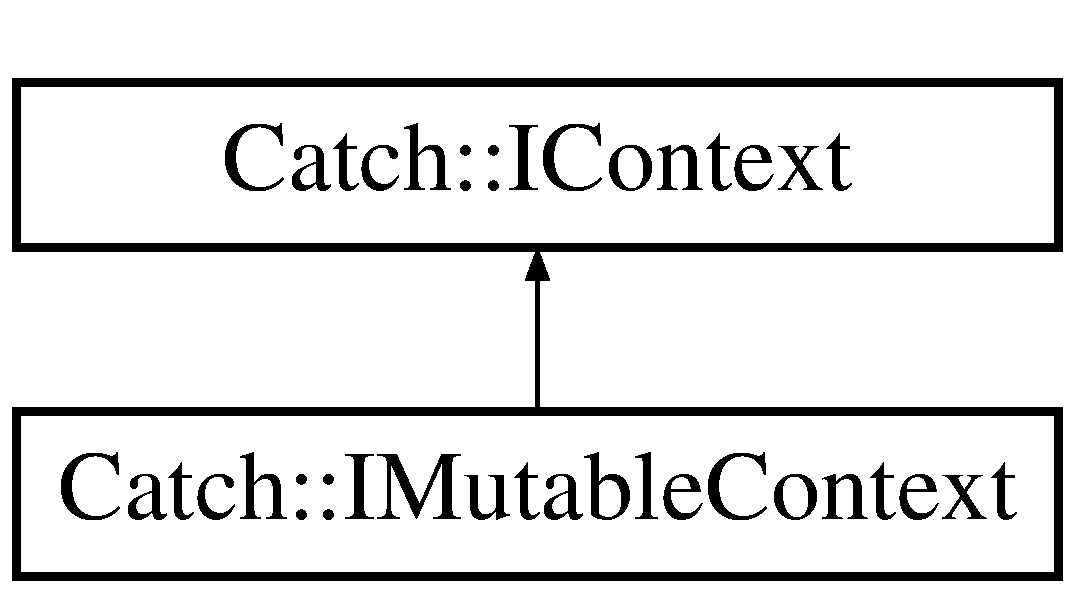
\includegraphics[height=2.000000cm]{structCatch_1_1IMutableContext}
\end{center}
\end{figure}
\subsection*{Public Member Functions}
\begin{DoxyCompactItemize}
\item 
virtual \hyperlink{structCatch_1_1IMutableContext_a93f32b2ab6d0fb83637059240be799ab}{$\sim$\-I\-Mutable\-Context} ()
\item 
virtual void \hyperlink{structCatch_1_1IMutableContext_a4a80afd0525b7def21bee8d9b48f2d39}{set\-Result\-Capture} (\hyperlink{structCatch_1_1IResultCapture}{I\-Result\-Capture} $\ast$result\-Capture)=0
\item 
virtual void \hyperlink{structCatch_1_1IMutableContext_af2e53b1dea4527a2587cff266a730f6e}{set\-Runner} (\hyperlink{structCatch_1_1IRunner}{I\-Runner} $\ast$runner)=0
\item 
virtual void \hyperlink{structCatch_1_1IMutableContext_a04ae4f4219a481a7bf658d9fd445bc1d}{set\-Config} (\hyperlink{classCatch_1_1Ptr}{Ptr}$<$ I\-Config const  $>$ const \&config)=0
\end{DoxyCompactItemize}


\subsection{Constructor \& Destructor Documentation}
\hypertarget{structCatch_1_1IMutableContext_a93f32b2ab6d0fb83637059240be799ab}{\index{Catch\-::\-I\-Mutable\-Context@{Catch\-::\-I\-Mutable\-Context}!$\sim$\-I\-Mutable\-Context@{$\sim$\-I\-Mutable\-Context}}
\index{$\sim$\-I\-Mutable\-Context@{$\sim$\-I\-Mutable\-Context}!Catch::IMutableContext@{Catch\-::\-I\-Mutable\-Context}}
\subsubsection[{$\sim$\-I\-Mutable\-Context}]{\setlength{\rightskip}{0pt plus 5cm}virtual Catch\-::\-I\-Mutable\-Context\-::$\sim$\-I\-Mutable\-Context (
\begin{DoxyParamCaption}
{}
\end{DoxyParamCaption}
)\hspace{0.3cm}{\ttfamily [virtual]}}}\label{structCatch_1_1IMutableContext_a93f32b2ab6d0fb83637059240be799ab}


\subsection{Member Function Documentation}
\hypertarget{structCatch_1_1IMutableContext_a04ae4f4219a481a7bf658d9fd445bc1d}{\index{Catch\-::\-I\-Mutable\-Context@{Catch\-::\-I\-Mutable\-Context}!set\-Config@{set\-Config}}
\index{set\-Config@{set\-Config}!Catch::IMutableContext@{Catch\-::\-I\-Mutable\-Context}}
\subsubsection[{set\-Config}]{\setlength{\rightskip}{0pt plus 5cm}virtual void Catch\-::\-I\-Mutable\-Context\-::set\-Config (
\begin{DoxyParamCaption}
\item[{{\bf Ptr}$<$ I\-Config const  $>$ const \&}]{config}
\end{DoxyParamCaption}
)\hspace{0.3cm}{\ttfamily [pure virtual]}}}\label{structCatch_1_1IMutableContext_a04ae4f4219a481a7bf658d9fd445bc1d}
\hypertarget{structCatch_1_1IMutableContext_a4a80afd0525b7def21bee8d9b48f2d39}{\index{Catch\-::\-I\-Mutable\-Context@{Catch\-::\-I\-Mutable\-Context}!set\-Result\-Capture@{set\-Result\-Capture}}
\index{set\-Result\-Capture@{set\-Result\-Capture}!Catch::IMutableContext@{Catch\-::\-I\-Mutable\-Context}}
\subsubsection[{set\-Result\-Capture}]{\setlength{\rightskip}{0pt plus 5cm}virtual void Catch\-::\-I\-Mutable\-Context\-::set\-Result\-Capture (
\begin{DoxyParamCaption}
\item[{{\bf I\-Result\-Capture} $\ast$}]{result\-Capture}
\end{DoxyParamCaption}
)\hspace{0.3cm}{\ttfamily [pure virtual]}}}\label{structCatch_1_1IMutableContext_a4a80afd0525b7def21bee8d9b48f2d39}
\hypertarget{structCatch_1_1IMutableContext_af2e53b1dea4527a2587cff266a730f6e}{\index{Catch\-::\-I\-Mutable\-Context@{Catch\-::\-I\-Mutable\-Context}!set\-Runner@{set\-Runner}}
\index{set\-Runner@{set\-Runner}!Catch::IMutableContext@{Catch\-::\-I\-Mutable\-Context}}
\subsubsection[{set\-Runner}]{\setlength{\rightskip}{0pt plus 5cm}virtual void Catch\-::\-I\-Mutable\-Context\-::set\-Runner (
\begin{DoxyParamCaption}
\item[{{\bf I\-Runner} $\ast$}]{runner}
\end{DoxyParamCaption}
)\hspace{0.3cm}{\ttfamily [pure virtual]}}}\label{structCatch_1_1IMutableContext_af2e53b1dea4527a2587cff266a730f6e}


The documentation for this struct was generated from the following file\-:\begin{DoxyCompactItemize}
\item 
/home/alexander/\-Un\-B/\-M\-P/\-Trabalho\-\_\-2\-\_\-\-M\-P\-\_\-\-Alexander\-\_\-13\-\_\-0039853/include/\hyperlink{catch_8hpp}{catch.\-hpp}\end{DoxyCompactItemize}

\hypertarget{structCatch_1_1IMutableRegistryHub}{\section{Catch\-:\-:I\-Mutable\-Registry\-Hub Struct Reference}
\label{structCatch_1_1IMutableRegistryHub}\index{Catch\-::\-I\-Mutable\-Registry\-Hub@{Catch\-::\-I\-Mutable\-Registry\-Hub}}
}


{\ttfamily \#include $<$catch.\-hpp$>$}

\subsection*{Public Member Functions}
\begin{DoxyCompactItemize}
\item 
virtual \hyperlink{structCatch_1_1IMutableRegistryHub_a759ca1e044e19f905fb4d306f1367193}{$\sim$\-I\-Mutable\-Registry\-Hub} ()
\item 
virtual void \hyperlink{structCatch_1_1IMutableRegistryHub_aab72d0aa1fa14627f1a6a4c893ae0a12}{register\-Reporter} (std\-::string const \&name, \hyperlink{classCatch_1_1Ptr}{Ptr}$<$ I\-Reporter\-Factory $>$ const \&factory)=0
\item 
virtual void \hyperlink{structCatch_1_1IMutableRegistryHub_ae06fcb90ba3f2b389d450cd81e229276}{register\-Listener} (\hyperlink{classCatch_1_1Ptr}{Ptr}$<$ I\-Reporter\-Factory $>$ const \&factory)=0
\item 
virtual void \hyperlink{structCatch_1_1IMutableRegistryHub_a11b85c6744d88c9f83fe16ad4a8dd451}{register\-Test} (\hyperlink{classCatch_1_1TestCase}{Test\-Case} const \&test\-Info)=0
\item 
virtual void \hyperlink{structCatch_1_1IMutableRegistryHub_ae6825365102693cf7707db022a2c2b49}{register\-Translator} (const \hyperlink{structCatch_1_1IExceptionTranslator}{I\-Exception\-Translator} $\ast$translator)=0
\item 
virtual void \hyperlink{structCatch_1_1IMutableRegistryHub_abf2e386b6f94f615719ada711adbf822}{register\-Tag\-Alias} (std\-::string const \&alias, std\-::string const \&tag, \hyperlink{structCatch_1_1SourceLineInfo}{Source\-Line\-Info} const \&line\-Info)=0
\end{DoxyCompactItemize}


\subsection{Constructor \& Destructor Documentation}
\hypertarget{structCatch_1_1IMutableRegistryHub_a759ca1e044e19f905fb4d306f1367193}{\index{Catch\-::\-I\-Mutable\-Registry\-Hub@{Catch\-::\-I\-Mutable\-Registry\-Hub}!$\sim$\-I\-Mutable\-Registry\-Hub@{$\sim$\-I\-Mutable\-Registry\-Hub}}
\index{$\sim$\-I\-Mutable\-Registry\-Hub@{$\sim$\-I\-Mutable\-Registry\-Hub}!Catch::IMutableRegistryHub@{Catch\-::\-I\-Mutable\-Registry\-Hub}}
\subsubsection[{$\sim$\-I\-Mutable\-Registry\-Hub}]{\setlength{\rightskip}{0pt plus 5cm}virtual Catch\-::\-I\-Mutable\-Registry\-Hub\-::$\sim$\-I\-Mutable\-Registry\-Hub (
\begin{DoxyParamCaption}
{}
\end{DoxyParamCaption}
)\hspace{0.3cm}{\ttfamily [virtual]}}}\label{structCatch_1_1IMutableRegistryHub_a759ca1e044e19f905fb4d306f1367193}


\subsection{Member Function Documentation}
\hypertarget{structCatch_1_1IMutableRegistryHub_ae06fcb90ba3f2b389d450cd81e229276}{\index{Catch\-::\-I\-Mutable\-Registry\-Hub@{Catch\-::\-I\-Mutable\-Registry\-Hub}!register\-Listener@{register\-Listener}}
\index{register\-Listener@{register\-Listener}!Catch::IMutableRegistryHub@{Catch\-::\-I\-Mutable\-Registry\-Hub}}
\subsubsection[{register\-Listener}]{\setlength{\rightskip}{0pt plus 5cm}virtual void Catch\-::\-I\-Mutable\-Registry\-Hub\-::register\-Listener (
\begin{DoxyParamCaption}
\item[{{\bf Ptr}$<$ I\-Reporter\-Factory $>$ const \&}]{factory}
\end{DoxyParamCaption}
)\hspace{0.3cm}{\ttfamily [pure virtual]}}}\label{structCatch_1_1IMutableRegistryHub_ae06fcb90ba3f2b389d450cd81e229276}
\hypertarget{structCatch_1_1IMutableRegistryHub_aab72d0aa1fa14627f1a6a4c893ae0a12}{\index{Catch\-::\-I\-Mutable\-Registry\-Hub@{Catch\-::\-I\-Mutable\-Registry\-Hub}!register\-Reporter@{register\-Reporter}}
\index{register\-Reporter@{register\-Reporter}!Catch::IMutableRegistryHub@{Catch\-::\-I\-Mutable\-Registry\-Hub}}
\subsubsection[{register\-Reporter}]{\setlength{\rightskip}{0pt plus 5cm}virtual void Catch\-::\-I\-Mutable\-Registry\-Hub\-::register\-Reporter (
\begin{DoxyParamCaption}
\item[{std\-::string const \&}]{name, }
\item[{{\bf Ptr}$<$ I\-Reporter\-Factory $>$ const \&}]{factory}
\end{DoxyParamCaption}
)\hspace{0.3cm}{\ttfamily [pure virtual]}}}\label{structCatch_1_1IMutableRegistryHub_aab72d0aa1fa14627f1a6a4c893ae0a12}
\hypertarget{structCatch_1_1IMutableRegistryHub_abf2e386b6f94f615719ada711adbf822}{\index{Catch\-::\-I\-Mutable\-Registry\-Hub@{Catch\-::\-I\-Mutable\-Registry\-Hub}!register\-Tag\-Alias@{register\-Tag\-Alias}}
\index{register\-Tag\-Alias@{register\-Tag\-Alias}!Catch::IMutableRegistryHub@{Catch\-::\-I\-Mutable\-Registry\-Hub}}
\subsubsection[{register\-Tag\-Alias}]{\setlength{\rightskip}{0pt plus 5cm}virtual void Catch\-::\-I\-Mutable\-Registry\-Hub\-::register\-Tag\-Alias (
\begin{DoxyParamCaption}
\item[{std\-::string const \&}]{alias, }
\item[{std\-::string const \&}]{tag, }
\item[{{\bf Source\-Line\-Info} const \&}]{line\-Info}
\end{DoxyParamCaption}
)\hspace{0.3cm}{\ttfamily [pure virtual]}}}\label{structCatch_1_1IMutableRegistryHub_abf2e386b6f94f615719ada711adbf822}
\hypertarget{structCatch_1_1IMutableRegistryHub_a11b85c6744d88c9f83fe16ad4a8dd451}{\index{Catch\-::\-I\-Mutable\-Registry\-Hub@{Catch\-::\-I\-Mutable\-Registry\-Hub}!register\-Test@{register\-Test}}
\index{register\-Test@{register\-Test}!Catch::IMutableRegistryHub@{Catch\-::\-I\-Mutable\-Registry\-Hub}}
\subsubsection[{register\-Test}]{\setlength{\rightskip}{0pt plus 5cm}virtual void Catch\-::\-I\-Mutable\-Registry\-Hub\-::register\-Test (
\begin{DoxyParamCaption}
\item[{{\bf Test\-Case} const \&}]{test\-Info}
\end{DoxyParamCaption}
)\hspace{0.3cm}{\ttfamily [pure virtual]}}}\label{structCatch_1_1IMutableRegistryHub_a11b85c6744d88c9f83fe16ad4a8dd451}
\hypertarget{structCatch_1_1IMutableRegistryHub_ae6825365102693cf7707db022a2c2b49}{\index{Catch\-::\-I\-Mutable\-Registry\-Hub@{Catch\-::\-I\-Mutable\-Registry\-Hub}!register\-Translator@{register\-Translator}}
\index{register\-Translator@{register\-Translator}!Catch::IMutableRegistryHub@{Catch\-::\-I\-Mutable\-Registry\-Hub}}
\subsubsection[{register\-Translator}]{\setlength{\rightskip}{0pt plus 5cm}virtual void Catch\-::\-I\-Mutable\-Registry\-Hub\-::register\-Translator (
\begin{DoxyParamCaption}
\item[{const {\bf I\-Exception\-Translator} $\ast$}]{translator}
\end{DoxyParamCaption}
)\hspace{0.3cm}{\ttfamily [pure virtual]}}}\label{structCatch_1_1IMutableRegistryHub_ae6825365102693cf7707db022a2c2b49}


The documentation for this struct was generated from the following file\-:\begin{DoxyCompactItemize}
\item 
/home/alexander/\-Un\-B/\-M\-P/\-Trabalho\-\_\-2\-\_\-\-M\-P\-\_\-\-Alexander\-\_\-13\-\_\-0039853/include/\hyperlink{catch_8hpp}{catch.\-hpp}\end{DoxyCompactItemize}

\hypertarget{structCatch_1_1IRegistryHub}{\section{Catch\-:\-:I\-Registry\-Hub Struct Reference}
\label{structCatch_1_1IRegistryHub}\index{Catch\-::\-I\-Registry\-Hub@{Catch\-::\-I\-Registry\-Hub}}
}


{\ttfamily \#include $<$catch.\-hpp$>$}

\subsection*{Public Member Functions}
\begin{DoxyCompactItemize}
\item 
virtual \hyperlink{structCatch_1_1IRegistryHub_a050de0f27f96888c8b410992146c9a09}{$\sim$\-I\-Registry\-Hub} ()
\item 
virtual I\-Reporter\-Registry const \& \hyperlink{structCatch_1_1IRegistryHub_a55534563f7ecf7e20ec1e37285ebe54d}{get\-Reporter\-Registry} () const =0
\item 
virtual \hyperlink{structCatch_1_1ITestCaseRegistry}{I\-Test\-Case\-Registry} const \& \hyperlink{structCatch_1_1IRegistryHub_af4f6255f0c0f8f1f179fa9d7d4843076}{get\-Test\-Case\-Registry} () const =0
\item 
virtual \hyperlink{structCatch_1_1ITagAliasRegistry}{I\-Tag\-Alias\-Registry} const \& \hyperlink{structCatch_1_1IRegistryHub_a3c511b1d33e5a6d95c333a0ff387df1a}{get\-Tag\-Alias\-Registry} () const =0
\item 
virtual \\*
\hyperlink{structCatch_1_1IExceptionTranslatorRegistry}{I\-Exception\-Translator\-Registry} \& \hyperlink{structCatch_1_1IRegistryHub_a3606988da110c016c5af3ae63454eb78}{get\-Exception\-Translator\-Registry} ()=0
\end{DoxyCompactItemize}


\subsection{Constructor \& Destructor Documentation}
\hypertarget{structCatch_1_1IRegistryHub_a050de0f27f96888c8b410992146c9a09}{\index{Catch\-::\-I\-Registry\-Hub@{Catch\-::\-I\-Registry\-Hub}!$\sim$\-I\-Registry\-Hub@{$\sim$\-I\-Registry\-Hub}}
\index{$\sim$\-I\-Registry\-Hub@{$\sim$\-I\-Registry\-Hub}!Catch::IRegistryHub@{Catch\-::\-I\-Registry\-Hub}}
\subsubsection[{$\sim$\-I\-Registry\-Hub}]{\setlength{\rightskip}{0pt plus 5cm}virtual Catch\-::\-I\-Registry\-Hub\-::$\sim$\-I\-Registry\-Hub (
\begin{DoxyParamCaption}
{}
\end{DoxyParamCaption}
)\hspace{0.3cm}{\ttfamily [virtual]}}}\label{structCatch_1_1IRegistryHub_a050de0f27f96888c8b410992146c9a09}


\subsection{Member Function Documentation}
\hypertarget{structCatch_1_1IRegistryHub_a3606988da110c016c5af3ae63454eb78}{\index{Catch\-::\-I\-Registry\-Hub@{Catch\-::\-I\-Registry\-Hub}!get\-Exception\-Translator\-Registry@{get\-Exception\-Translator\-Registry}}
\index{get\-Exception\-Translator\-Registry@{get\-Exception\-Translator\-Registry}!Catch::IRegistryHub@{Catch\-::\-I\-Registry\-Hub}}
\subsubsection[{get\-Exception\-Translator\-Registry}]{\setlength{\rightskip}{0pt plus 5cm}virtual {\bf I\-Exception\-Translator\-Registry}\& Catch\-::\-I\-Registry\-Hub\-::get\-Exception\-Translator\-Registry (
\begin{DoxyParamCaption}
{}
\end{DoxyParamCaption}
)\hspace{0.3cm}{\ttfamily [pure virtual]}}}\label{structCatch_1_1IRegistryHub_a3606988da110c016c5af3ae63454eb78}
\hypertarget{structCatch_1_1IRegistryHub_a55534563f7ecf7e20ec1e37285ebe54d}{\index{Catch\-::\-I\-Registry\-Hub@{Catch\-::\-I\-Registry\-Hub}!get\-Reporter\-Registry@{get\-Reporter\-Registry}}
\index{get\-Reporter\-Registry@{get\-Reporter\-Registry}!Catch::IRegistryHub@{Catch\-::\-I\-Registry\-Hub}}
\subsubsection[{get\-Reporter\-Registry}]{\setlength{\rightskip}{0pt plus 5cm}virtual I\-Reporter\-Registry const\& Catch\-::\-I\-Registry\-Hub\-::get\-Reporter\-Registry (
\begin{DoxyParamCaption}
{}
\end{DoxyParamCaption}
) const\hspace{0.3cm}{\ttfamily [pure virtual]}}}\label{structCatch_1_1IRegistryHub_a55534563f7ecf7e20ec1e37285ebe54d}
\hypertarget{structCatch_1_1IRegistryHub_a3c511b1d33e5a6d95c333a0ff387df1a}{\index{Catch\-::\-I\-Registry\-Hub@{Catch\-::\-I\-Registry\-Hub}!get\-Tag\-Alias\-Registry@{get\-Tag\-Alias\-Registry}}
\index{get\-Tag\-Alias\-Registry@{get\-Tag\-Alias\-Registry}!Catch::IRegistryHub@{Catch\-::\-I\-Registry\-Hub}}
\subsubsection[{get\-Tag\-Alias\-Registry}]{\setlength{\rightskip}{0pt plus 5cm}virtual {\bf I\-Tag\-Alias\-Registry} const\& Catch\-::\-I\-Registry\-Hub\-::get\-Tag\-Alias\-Registry (
\begin{DoxyParamCaption}
{}
\end{DoxyParamCaption}
) const\hspace{0.3cm}{\ttfamily [pure virtual]}}}\label{structCatch_1_1IRegistryHub_a3c511b1d33e5a6d95c333a0ff387df1a}
\hypertarget{structCatch_1_1IRegistryHub_af4f6255f0c0f8f1f179fa9d7d4843076}{\index{Catch\-::\-I\-Registry\-Hub@{Catch\-::\-I\-Registry\-Hub}!get\-Test\-Case\-Registry@{get\-Test\-Case\-Registry}}
\index{get\-Test\-Case\-Registry@{get\-Test\-Case\-Registry}!Catch::IRegistryHub@{Catch\-::\-I\-Registry\-Hub}}
\subsubsection[{get\-Test\-Case\-Registry}]{\setlength{\rightskip}{0pt plus 5cm}virtual {\bf I\-Test\-Case\-Registry} const\& Catch\-::\-I\-Registry\-Hub\-::get\-Test\-Case\-Registry (
\begin{DoxyParamCaption}
{}
\end{DoxyParamCaption}
) const\hspace{0.3cm}{\ttfamily [pure virtual]}}}\label{structCatch_1_1IRegistryHub_af4f6255f0c0f8f1f179fa9d7d4843076}


The documentation for this struct was generated from the following file\-:\begin{DoxyCompactItemize}
\item 
/home/alexander/\-Un\-B/\-M\-P/\-Trabalho\-\_\-2\-\_\-\-M\-P\-\_\-\-Alexander\-\_\-13\-\_\-0039853/include/\hyperlink{catch_8hpp}{catch.\-hpp}\end{DoxyCompactItemize}

\hypertarget{structCatch_1_1IResultCapture}{\section{Catch\-:\-:I\-Result\-Capture Struct Reference}
\label{structCatch_1_1IResultCapture}\index{Catch\-::\-I\-Result\-Capture@{Catch\-::\-I\-Result\-Capture}}
}


{\ttfamily \#include $<$catch.\-hpp$>$}

\subsection*{Public Member Functions}
\begin{DoxyCompactItemize}
\item 
virtual \hyperlink{structCatch_1_1IResultCapture_a3bd16719d6772b7470887fc36c6d0808}{$\sim$\-I\-Result\-Capture} ()
\item 
virtual void \hyperlink{structCatch_1_1IResultCapture_ae45e08bccc5fb434656d4f2e44742223}{assertion\-Ended} (\hyperlink{classCatch_1_1AssertionResult}{Assertion\-Result} const \&result)=0
\item 
virtual bool \hyperlink{structCatch_1_1IResultCapture_a5b76ed52badcb64cf374202e12b81a03}{section\-Started} (\hyperlink{structCatch_1_1SectionInfo}{Section\-Info} const \&section\-Info, \hyperlink{structCatch_1_1Counts}{Counts} \&assertions)=0
\item 
virtual void \hyperlink{structCatch_1_1IResultCapture_a4e152bc43dc0933684e31fa67a58195d}{section\-Ended} (\hyperlink{structCatch_1_1SectionEndInfo}{Section\-End\-Info} const \&end\-Info)=0
\item 
virtual void \hyperlink{structCatch_1_1IResultCapture_afcc71eef8ca821ae132cced4a2be6988}{section\-Ended\-Early} (\hyperlink{structCatch_1_1SectionEndInfo}{Section\-End\-Info} const \&end\-Info)=0
\item 
virtual void \hyperlink{structCatch_1_1IResultCapture_a91d154c1e087e383dcde5aad95cb6a05}{push\-Scoped\-Message} (\hyperlink{structCatch_1_1MessageInfo}{Message\-Info} const \&message)=0
\item 
virtual void \hyperlink{structCatch_1_1IResultCapture_a42bcb13276706bf8c3ce081ce16d37fd}{pop\-Scoped\-Message} (\hyperlink{structCatch_1_1MessageInfo}{Message\-Info} const \&message)=0
\item 
virtual std\-::string \hyperlink{structCatch_1_1IResultCapture_aea1617f4a84cc648246aa3ed6918b5bf}{get\-Current\-Test\-Name} () const =0
\item 
virtual const \hyperlink{classCatch_1_1AssertionResult}{Assertion\-Result} $\ast$ \hyperlink{structCatch_1_1IResultCapture_ab18872c89fab97405a56e9c6a4919736}{get\-Last\-Result} () const =0
\item 
virtual void \hyperlink{structCatch_1_1IResultCapture_ae63ecec95db4c236c63ecf616f483810}{exception\-Early\-Reported} ()=0
\item 
virtual void \hyperlink{structCatch_1_1IResultCapture_a7d995222301e6605f26549726b30c3ee}{handle\-Fatal\-Error\-Condition} (std\-::string const \&message)=0
\end{DoxyCompactItemize}


\subsection{Constructor \& Destructor Documentation}
\hypertarget{structCatch_1_1IResultCapture_a3bd16719d6772b7470887fc36c6d0808}{\index{Catch\-::\-I\-Result\-Capture@{Catch\-::\-I\-Result\-Capture}!$\sim$\-I\-Result\-Capture@{$\sim$\-I\-Result\-Capture}}
\index{$\sim$\-I\-Result\-Capture@{$\sim$\-I\-Result\-Capture}!Catch::IResultCapture@{Catch\-::\-I\-Result\-Capture}}
\subsubsection[{$\sim$\-I\-Result\-Capture}]{\setlength{\rightskip}{0pt plus 5cm}virtual Catch\-::\-I\-Result\-Capture\-::$\sim$\-I\-Result\-Capture (
\begin{DoxyParamCaption}
{}
\end{DoxyParamCaption}
)\hspace{0.3cm}{\ttfamily [virtual]}}}\label{structCatch_1_1IResultCapture_a3bd16719d6772b7470887fc36c6d0808}


\subsection{Member Function Documentation}
\hypertarget{structCatch_1_1IResultCapture_ae45e08bccc5fb434656d4f2e44742223}{\index{Catch\-::\-I\-Result\-Capture@{Catch\-::\-I\-Result\-Capture}!assertion\-Ended@{assertion\-Ended}}
\index{assertion\-Ended@{assertion\-Ended}!Catch::IResultCapture@{Catch\-::\-I\-Result\-Capture}}
\subsubsection[{assertion\-Ended}]{\setlength{\rightskip}{0pt plus 5cm}virtual void Catch\-::\-I\-Result\-Capture\-::assertion\-Ended (
\begin{DoxyParamCaption}
\item[{{\bf Assertion\-Result} const \&}]{result}
\end{DoxyParamCaption}
)\hspace{0.3cm}{\ttfamily [pure virtual]}}}\label{structCatch_1_1IResultCapture_ae45e08bccc5fb434656d4f2e44742223}
\hypertarget{structCatch_1_1IResultCapture_ae63ecec95db4c236c63ecf616f483810}{\index{Catch\-::\-I\-Result\-Capture@{Catch\-::\-I\-Result\-Capture}!exception\-Early\-Reported@{exception\-Early\-Reported}}
\index{exception\-Early\-Reported@{exception\-Early\-Reported}!Catch::IResultCapture@{Catch\-::\-I\-Result\-Capture}}
\subsubsection[{exception\-Early\-Reported}]{\setlength{\rightskip}{0pt plus 5cm}virtual void Catch\-::\-I\-Result\-Capture\-::exception\-Early\-Reported (
\begin{DoxyParamCaption}
{}
\end{DoxyParamCaption}
)\hspace{0.3cm}{\ttfamily [pure virtual]}}}\label{structCatch_1_1IResultCapture_ae63ecec95db4c236c63ecf616f483810}
\hypertarget{structCatch_1_1IResultCapture_aea1617f4a84cc648246aa3ed6918b5bf}{\index{Catch\-::\-I\-Result\-Capture@{Catch\-::\-I\-Result\-Capture}!get\-Current\-Test\-Name@{get\-Current\-Test\-Name}}
\index{get\-Current\-Test\-Name@{get\-Current\-Test\-Name}!Catch::IResultCapture@{Catch\-::\-I\-Result\-Capture}}
\subsubsection[{get\-Current\-Test\-Name}]{\setlength{\rightskip}{0pt plus 5cm}virtual std\-::string Catch\-::\-I\-Result\-Capture\-::get\-Current\-Test\-Name (
\begin{DoxyParamCaption}
{}
\end{DoxyParamCaption}
) const\hspace{0.3cm}{\ttfamily [pure virtual]}}}\label{structCatch_1_1IResultCapture_aea1617f4a84cc648246aa3ed6918b5bf}
\hypertarget{structCatch_1_1IResultCapture_ab18872c89fab97405a56e9c6a4919736}{\index{Catch\-::\-I\-Result\-Capture@{Catch\-::\-I\-Result\-Capture}!get\-Last\-Result@{get\-Last\-Result}}
\index{get\-Last\-Result@{get\-Last\-Result}!Catch::IResultCapture@{Catch\-::\-I\-Result\-Capture}}
\subsubsection[{get\-Last\-Result}]{\setlength{\rightskip}{0pt plus 5cm}virtual const {\bf Assertion\-Result}$\ast$ Catch\-::\-I\-Result\-Capture\-::get\-Last\-Result (
\begin{DoxyParamCaption}
{}
\end{DoxyParamCaption}
) const\hspace{0.3cm}{\ttfamily [pure virtual]}}}\label{structCatch_1_1IResultCapture_ab18872c89fab97405a56e9c6a4919736}
\hypertarget{structCatch_1_1IResultCapture_a7d995222301e6605f26549726b30c3ee}{\index{Catch\-::\-I\-Result\-Capture@{Catch\-::\-I\-Result\-Capture}!handle\-Fatal\-Error\-Condition@{handle\-Fatal\-Error\-Condition}}
\index{handle\-Fatal\-Error\-Condition@{handle\-Fatal\-Error\-Condition}!Catch::IResultCapture@{Catch\-::\-I\-Result\-Capture}}
\subsubsection[{handle\-Fatal\-Error\-Condition}]{\setlength{\rightskip}{0pt plus 5cm}virtual void Catch\-::\-I\-Result\-Capture\-::handle\-Fatal\-Error\-Condition (
\begin{DoxyParamCaption}
\item[{std\-::string const \&}]{message}
\end{DoxyParamCaption}
)\hspace{0.3cm}{\ttfamily [pure virtual]}}}\label{structCatch_1_1IResultCapture_a7d995222301e6605f26549726b30c3ee}
\hypertarget{structCatch_1_1IResultCapture_a42bcb13276706bf8c3ce081ce16d37fd}{\index{Catch\-::\-I\-Result\-Capture@{Catch\-::\-I\-Result\-Capture}!pop\-Scoped\-Message@{pop\-Scoped\-Message}}
\index{pop\-Scoped\-Message@{pop\-Scoped\-Message}!Catch::IResultCapture@{Catch\-::\-I\-Result\-Capture}}
\subsubsection[{pop\-Scoped\-Message}]{\setlength{\rightskip}{0pt plus 5cm}virtual void Catch\-::\-I\-Result\-Capture\-::pop\-Scoped\-Message (
\begin{DoxyParamCaption}
\item[{{\bf Message\-Info} const \&}]{message}
\end{DoxyParamCaption}
)\hspace{0.3cm}{\ttfamily [pure virtual]}}}\label{structCatch_1_1IResultCapture_a42bcb13276706bf8c3ce081ce16d37fd}
\hypertarget{structCatch_1_1IResultCapture_a91d154c1e087e383dcde5aad95cb6a05}{\index{Catch\-::\-I\-Result\-Capture@{Catch\-::\-I\-Result\-Capture}!push\-Scoped\-Message@{push\-Scoped\-Message}}
\index{push\-Scoped\-Message@{push\-Scoped\-Message}!Catch::IResultCapture@{Catch\-::\-I\-Result\-Capture}}
\subsubsection[{push\-Scoped\-Message}]{\setlength{\rightskip}{0pt plus 5cm}virtual void Catch\-::\-I\-Result\-Capture\-::push\-Scoped\-Message (
\begin{DoxyParamCaption}
\item[{{\bf Message\-Info} const \&}]{message}
\end{DoxyParamCaption}
)\hspace{0.3cm}{\ttfamily [pure virtual]}}}\label{structCatch_1_1IResultCapture_a91d154c1e087e383dcde5aad95cb6a05}
\hypertarget{structCatch_1_1IResultCapture_a4e152bc43dc0933684e31fa67a58195d}{\index{Catch\-::\-I\-Result\-Capture@{Catch\-::\-I\-Result\-Capture}!section\-Ended@{section\-Ended}}
\index{section\-Ended@{section\-Ended}!Catch::IResultCapture@{Catch\-::\-I\-Result\-Capture}}
\subsubsection[{section\-Ended}]{\setlength{\rightskip}{0pt plus 5cm}virtual void Catch\-::\-I\-Result\-Capture\-::section\-Ended (
\begin{DoxyParamCaption}
\item[{{\bf Section\-End\-Info} const \&}]{end\-Info}
\end{DoxyParamCaption}
)\hspace{0.3cm}{\ttfamily [pure virtual]}}}\label{structCatch_1_1IResultCapture_a4e152bc43dc0933684e31fa67a58195d}
\hypertarget{structCatch_1_1IResultCapture_afcc71eef8ca821ae132cced4a2be6988}{\index{Catch\-::\-I\-Result\-Capture@{Catch\-::\-I\-Result\-Capture}!section\-Ended\-Early@{section\-Ended\-Early}}
\index{section\-Ended\-Early@{section\-Ended\-Early}!Catch::IResultCapture@{Catch\-::\-I\-Result\-Capture}}
\subsubsection[{section\-Ended\-Early}]{\setlength{\rightskip}{0pt plus 5cm}virtual void Catch\-::\-I\-Result\-Capture\-::section\-Ended\-Early (
\begin{DoxyParamCaption}
\item[{{\bf Section\-End\-Info} const \&}]{end\-Info}
\end{DoxyParamCaption}
)\hspace{0.3cm}{\ttfamily [pure virtual]}}}\label{structCatch_1_1IResultCapture_afcc71eef8ca821ae132cced4a2be6988}
\hypertarget{structCatch_1_1IResultCapture_a5b76ed52badcb64cf374202e12b81a03}{\index{Catch\-::\-I\-Result\-Capture@{Catch\-::\-I\-Result\-Capture}!section\-Started@{section\-Started}}
\index{section\-Started@{section\-Started}!Catch::IResultCapture@{Catch\-::\-I\-Result\-Capture}}
\subsubsection[{section\-Started}]{\setlength{\rightskip}{0pt plus 5cm}virtual bool Catch\-::\-I\-Result\-Capture\-::section\-Started (
\begin{DoxyParamCaption}
\item[{{\bf Section\-Info} const \&}]{section\-Info, }
\item[{{\bf Counts} \&}]{assertions}
\end{DoxyParamCaption}
)\hspace{0.3cm}{\ttfamily [pure virtual]}}}\label{structCatch_1_1IResultCapture_a5b76ed52badcb64cf374202e12b81a03}


The documentation for this struct was generated from the following file\-:\begin{DoxyCompactItemize}
\item 
/home/alexander/\-Un\-B/\-M\-P/\-Trabalho\-\_\-2\-\_\-\-M\-P\-\_\-\-Alexander\-\_\-13\-\_\-0039853/include/\hyperlink{catch_8hpp}{catch.\-hpp}\end{DoxyCompactItemize}

\hypertarget{structCatch_1_1IRunner}{\section{Catch\-:\-:I\-Runner Struct Reference}
\label{structCatch_1_1IRunner}\index{Catch\-::\-I\-Runner@{Catch\-::\-I\-Runner}}
}


{\ttfamily \#include $<$catch.\-hpp$>$}

\subsection*{Public Member Functions}
\begin{DoxyCompactItemize}
\item 
virtual \hyperlink{structCatch_1_1IRunner_a5f539a88a7772d68de8a2e4028774209}{$\sim$\-I\-Runner} ()
\item 
virtual bool \hyperlink{structCatch_1_1IRunner_a03713202dd2e041e30b8030088ab0116}{aborting} () const =0
\end{DoxyCompactItemize}


\subsection{Constructor \& Destructor Documentation}
\hypertarget{structCatch_1_1IRunner_a5f539a88a7772d68de8a2e4028774209}{\index{Catch\-::\-I\-Runner@{Catch\-::\-I\-Runner}!$\sim$\-I\-Runner@{$\sim$\-I\-Runner}}
\index{$\sim$\-I\-Runner@{$\sim$\-I\-Runner}!Catch::IRunner@{Catch\-::\-I\-Runner}}
\subsubsection[{$\sim$\-I\-Runner}]{\setlength{\rightskip}{0pt plus 5cm}virtual Catch\-::\-I\-Runner\-::$\sim$\-I\-Runner (
\begin{DoxyParamCaption}
{}
\end{DoxyParamCaption}
)\hspace{0.3cm}{\ttfamily [virtual]}}}\label{structCatch_1_1IRunner_a5f539a88a7772d68de8a2e4028774209}


\subsection{Member Function Documentation}
\hypertarget{structCatch_1_1IRunner_a03713202dd2e041e30b8030088ab0116}{\index{Catch\-::\-I\-Runner@{Catch\-::\-I\-Runner}!aborting@{aborting}}
\index{aborting@{aborting}!Catch::IRunner@{Catch\-::\-I\-Runner}}
\subsubsection[{aborting}]{\setlength{\rightskip}{0pt plus 5cm}virtual bool Catch\-::\-I\-Runner\-::aborting (
\begin{DoxyParamCaption}
{}
\end{DoxyParamCaption}
) const\hspace{0.3cm}{\ttfamily [pure virtual]}}}\label{structCatch_1_1IRunner_a03713202dd2e041e30b8030088ab0116}


The documentation for this struct was generated from the following file\-:\begin{DoxyCompactItemize}
\item 
/home/alexander/\-Un\-B/\-M\-P/\-Trabalho\-\_\-2\-\_\-\-M\-P\-\_\-\-Alexander\-\_\-13\-\_\-0039853/include/\hyperlink{catch_8hpp}{catch.\-hpp}\end{DoxyCompactItemize}

\hypertarget{structCatch_1_1IShared}{\section{Catch\-:\-:I\-Shared Struct Reference}
\label{structCatch_1_1IShared}\index{Catch\-::\-I\-Shared@{Catch\-::\-I\-Shared}}
}


{\ttfamily \#include $<$catch.\-hpp$>$}

Inheritance diagram for Catch\-:\-:I\-Shared\-:\begin{figure}[H]
\begin{center}
\leavevmode
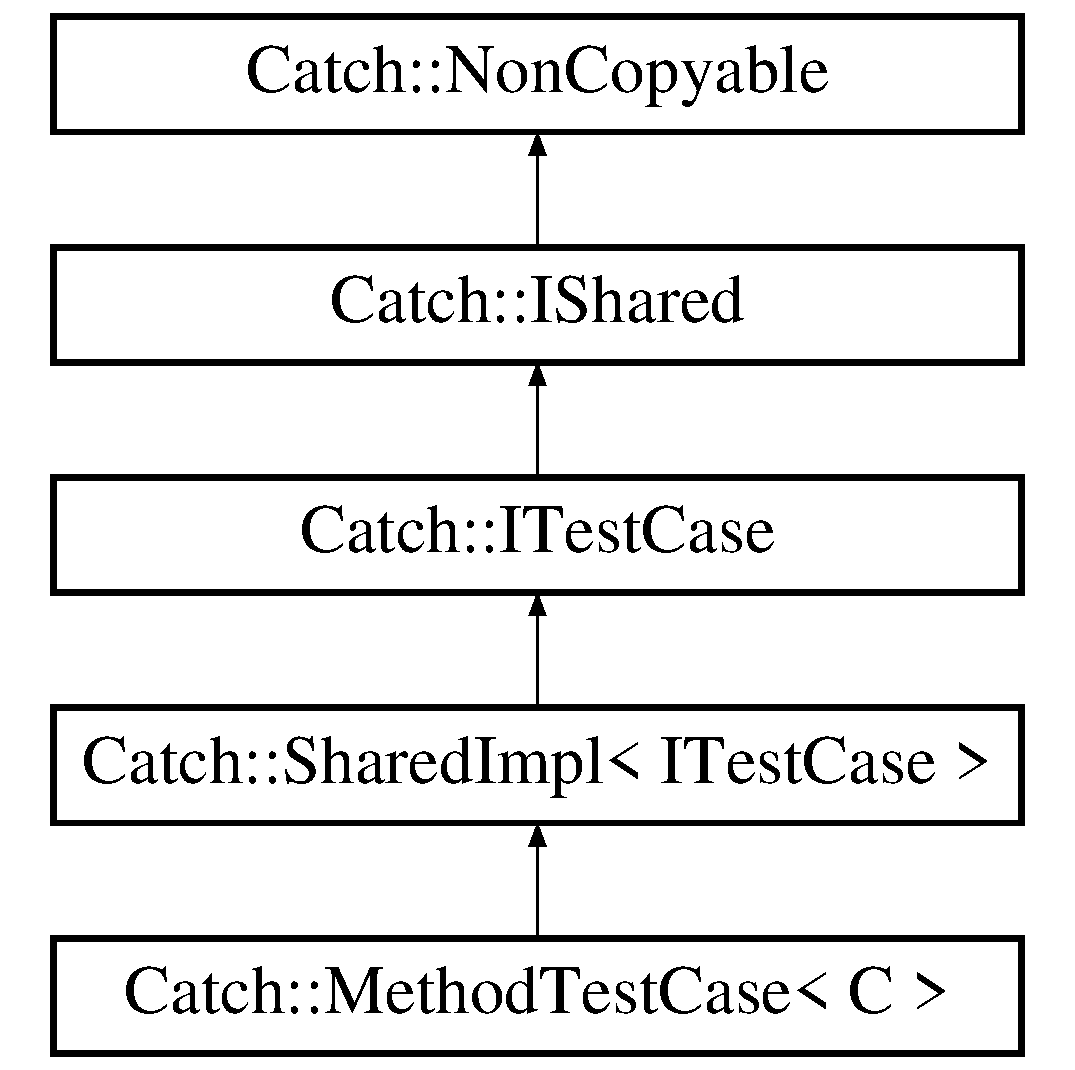
\includegraphics[height=5.000000cm]{structCatch_1_1IShared}
\end{center}
\end{figure}
\subsection*{Public Member Functions}
\begin{DoxyCompactItemize}
\item 
virtual \hyperlink{structCatch_1_1IShared_a5e842e7540ae7ae0c62a2758123503f6}{$\sim$\-I\-Shared} ()
\item 
virtual void \hyperlink{structCatch_1_1IShared_ae383df68557cdaf0910b411af04d9e33}{add\-Ref} () const =0
\item 
virtual void \hyperlink{structCatch_1_1IShared_a002f52624728a763956fb6f230cb2f57}{release} () const =0
\end{DoxyCompactItemize}
\subsection*{Additional Inherited Members}


\subsection{Constructor \& Destructor Documentation}
\hypertarget{structCatch_1_1IShared_a5e842e7540ae7ae0c62a2758123503f6}{\index{Catch\-::\-I\-Shared@{Catch\-::\-I\-Shared}!$\sim$\-I\-Shared@{$\sim$\-I\-Shared}}
\index{$\sim$\-I\-Shared@{$\sim$\-I\-Shared}!Catch::IShared@{Catch\-::\-I\-Shared}}
\subsubsection[{$\sim$\-I\-Shared}]{\setlength{\rightskip}{0pt plus 5cm}virtual Catch\-::\-I\-Shared\-::$\sim$\-I\-Shared (
\begin{DoxyParamCaption}
{}
\end{DoxyParamCaption}
)\hspace{0.3cm}{\ttfamily [virtual]}}}\label{structCatch_1_1IShared_a5e842e7540ae7ae0c62a2758123503f6}


\subsection{Member Function Documentation}
\hypertarget{structCatch_1_1IShared_ae383df68557cdaf0910b411af04d9e33}{\index{Catch\-::\-I\-Shared@{Catch\-::\-I\-Shared}!add\-Ref@{add\-Ref}}
\index{add\-Ref@{add\-Ref}!Catch::IShared@{Catch\-::\-I\-Shared}}
\subsubsection[{add\-Ref}]{\setlength{\rightskip}{0pt plus 5cm}virtual void Catch\-::\-I\-Shared\-::add\-Ref (
\begin{DoxyParamCaption}
{}
\end{DoxyParamCaption}
) const\hspace{0.3cm}{\ttfamily [pure virtual]}}}\label{structCatch_1_1IShared_ae383df68557cdaf0910b411af04d9e33}


Implemented in \hyperlink{structCatch_1_1SharedImpl_a9b190b7a139a09d2624d1201d8e4f87e}{Catch\-::\-Shared\-Impl$<$ I\-Test\-Case $>$}.

\hypertarget{structCatch_1_1IShared_a002f52624728a763956fb6f230cb2f57}{\index{Catch\-::\-I\-Shared@{Catch\-::\-I\-Shared}!release@{release}}
\index{release@{release}!Catch::IShared@{Catch\-::\-I\-Shared}}
\subsubsection[{release}]{\setlength{\rightskip}{0pt plus 5cm}virtual void Catch\-::\-I\-Shared\-::release (
\begin{DoxyParamCaption}
{}
\end{DoxyParamCaption}
) const\hspace{0.3cm}{\ttfamily [pure virtual]}}}\label{structCatch_1_1IShared_a002f52624728a763956fb6f230cb2f57}


Implemented in \hyperlink{structCatch_1_1SharedImpl_a16baad80ad5ad3dfaf2a10a157a02e01}{Catch\-::\-Shared\-Impl$<$ I\-Test\-Case $>$}.



The documentation for this struct was generated from the following file\-:\begin{DoxyCompactItemize}
\item 
/home/alexander/\-Un\-B/\-M\-P/\-Trabalho\-\_\-2\-\_\-\-M\-P\-\_\-\-Alexander\-\_\-13\-\_\-0039853/include/\hyperlink{catch_8hpp}{catch.\-hpp}\end{DoxyCompactItemize}

\hypertarget{structCatch_1_1Detail_1_1IsStreamInsertable}{\section{Catch\-:\-:Detail\-:\-:Is\-Stream\-Insertable$<$ T $>$ Struct Template Reference}
\label{structCatch_1_1Detail_1_1IsStreamInsertable}\index{Catch\-::\-Detail\-::\-Is\-Stream\-Insertable$<$ T $>$@{Catch\-::\-Detail\-::\-Is\-Stream\-Insertable$<$ T $>$}}
}


{\ttfamily \#include $<$catch.\-hpp$>$}

\subsection*{Public Types}
\begin{DoxyCompactItemize}
\item 
enum \{ \hyperlink{structCatch_1_1Detail_1_1IsStreamInsertable_a2e4508694da3bf368ff67733a7970edda765a324929702bfce2969fc19fc4f926}{value} = sizeof( test\-Streamable(s $<$$<$ t) ) == sizeof( True\-Type )
 \}
\end{DoxyCompactItemize}
\subsection*{Static Public Attributes}
\begin{DoxyCompactItemize}
\item 
static std\-::ostream \& \hyperlink{structCatch_1_1Detail_1_1IsStreamInsertable_abe3d3c8e5d85665747faafffc9a96b00}{s}
\item 
static T const \& \hyperlink{structCatch_1_1Detail_1_1IsStreamInsertable_a7d2a3da978b6736667a7b2f6d51f507f}{t}
\end{DoxyCompactItemize}


\subsection{Member Enumeration Documentation}
\hypertarget{structCatch_1_1Detail_1_1IsStreamInsertable_a2e4508694da3bf368ff67733a7970edd}{\subsubsection[{anonymous enum}]{\setlength{\rightskip}{0pt plus 5cm}template$<$typename T $>$ anonymous enum}}\label{structCatch_1_1Detail_1_1IsStreamInsertable_a2e4508694da3bf368ff67733a7970edd}
\begin{Desc}
\item[Enumerator]\par
\begin{description}
\index{value@{value}!Catch\-::\-Detail\-::\-Is\-Stream\-Insertable@{Catch\-::\-Detail\-::\-Is\-Stream\-Insertable}}\index{Catch\-::\-Detail\-::\-Is\-Stream\-Insertable@{Catch\-::\-Detail\-::\-Is\-Stream\-Insertable}!value@{value}}\item[{\em 
\hypertarget{structCatch_1_1Detail_1_1IsStreamInsertable_a2e4508694da3bf368ff67733a7970edda765a324929702bfce2969fc19fc4f926}{value}\label{structCatch_1_1Detail_1_1IsStreamInsertable_a2e4508694da3bf368ff67733a7970edda765a324929702bfce2969fc19fc4f926}
}]\end{description}
\end{Desc}


\subsection{Member Data Documentation}
\hypertarget{structCatch_1_1Detail_1_1IsStreamInsertable_abe3d3c8e5d85665747faafffc9a96b00}{\index{Catch\-::\-Detail\-::\-Is\-Stream\-Insertable@{Catch\-::\-Detail\-::\-Is\-Stream\-Insertable}!s@{s}}
\index{s@{s}!Catch::Detail::IsStreamInsertable@{Catch\-::\-Detail\-::\-Is\-Stream\-Insertable}}
\subsubsection[{s}]{\setlength{\rightskip}{0pt plus 5cm}template$<$typename T $>$ std\-::ostream\& {\bf Catch\-::\-Detail\-::\-Is\-Stream\-Insertable}$<$ T $>$\-::s\hspace{0.3cm}{\ttfamily [static]}}}\label{structCatch_1_1Detail_1_1IsStreamInsertable_abe3d3c8e5d85665747faafffc9a96b00}
\hypertarget{structCatch_1_1Detail_1_1IsStreamInsertable_a7d2a3da978b6736667a7b2f6d51f507f}{\index{Catch\-::\-Detail\-::\-Is\-Stream\-Insertable@{Catch\-::\-Detail\-::\-Is\-Stream\-Insertable}!t@{t}}
\index{t@{t}!Catch::Detail::IsStreamInsertable@{Catch\-::\-Detail\-::\-Is\-Stream\-Insertable}}
\subsubsection[{t}]{\setlength{\rightskip}{0pt plus 5cm}template$<$typename T $>$ T const\& {\bf Catch\-::\-Detail\-::\-Is\-Stream\-Insertable}$<$ T $>$\-::t\hspace{0.3cm}{\ttfamily [static]}}}\label{structCatch_1_1Detail_1_1IsStreamInsertable_a7d2a3da978b6736667a7b2f6d51f507f}


The documentation for this struct was generated from the following file\-:\begin{DoxyCompactItemize}
\item 
/home/alexander/\-Un\-B/\-M\-P/\-Trabalho\-\_\-2\-\_\-\-M\-P\-\_\-\-Alexander\-\_\-13\-\_\-0039853/include/\hyperlink{catch_8hpp}{catch.\-hpp}\end{DoxyCompactItemize}

\hypertarget{structCatch_1_1ITagAliasRegistry}{\section{Catch\-:\-:I\-Tag\-Alias\-Registry Struct Reference}
\label{structCatch_1_1ITagAliasRegistry}\index{Catch\-::\-I\-Tag\-Alias\-Registry@{Catch\-::\-I\-Tag\-Alias\-Registry}}
}


{\ttfamily \#include $<$catch.\-hpp$>$}

\subsection*{Public Member Functions}
\begin{DoxyCompactItemize}
\item 
virtual \hyperlink{structCatch_1_1ITagAliasRegistry_a8967db4dd40b68e22697eff0f4928239}{$\sim$\-I\-Tag\-Alias\-Registry} ()
\item 
virtual \hyperlink{classCatch_1_1Option}{Option}$<$ \hyperlink{structCatch_1_1TagAlias}{Tag\-Alias} $>$ \hyperlink{structCatch_1_1ITagAliasRegistry_a7d2fba4d39cfcc62c2695fcde4f989c3}{find} (std\-::string const \&alias) const =0
\item 
virtual std\-::string \hyperlink{structCatch_1_1ITagAliasRegistry_ae729a7532faf7466db1a157ce0395170}{expand\-Aliases} (std\-::string const \&unexpanded\-Test\-Spec) const =0
\end{DoxyCompactItemize}
\subsection*{Static Public Member Functions}
\begin{DoxyCompactItemize}
\item 
static \hyperlink{structCatch_1_1ITagAliasRegistry}{I\-Tag\-Alias\-Registry} const \& \hyperlink{structCatch_1_1ITagAliasRegistry_aa9d0f008f49473389c7abf6071f137a7}{get} ()
\end{DoxyCompactItemize}


\subsection{Constructor \& Destructor Documentation}
\hypertarget{structCatch_1_1ITagAliasRegistry_a8967db4dd40b68e22697eff0f4928239}{\index{Catch\-::\-I\-Tag\-Alias\-Registry@{Catch\-::\-I\-Tag\-Alias\-Registry}!$\sim$\-I\-Tag\-Alias\-Registry@{$\sim$\-I\-Tag\-Alias\-Registry}}
\index{$\sim$\-I\-Tag\-Alias\-Registry@{$\sim$\-I\-Tag\-Alias\-Registry}!Catch::ITagAliasRegistry@{Catch\-::\-I\-Tag\-Alias\-Registry}}
\subsubsection[{$\sim$\-I\-Tag\-Alias\-Registry}]{\setlength{\rightskip}{0pt plus 5cm}virtual Catch\-::\-I\-Tag\-Alias\-Registry\-::$\sim$\-I\-Tag\-Alias\-Registry (
\begin{DoxyParamCaption}
{}
\end{DoxyParamCaption}
)\hspace{0.3cm}{\ttfamily [virtual]}}}\label{structCatch_1_1ITagAliasRegistry_a8967db4dd40b68e22697eff0f4928239}


\subsection{Member Function Documentation}
\hypertarget{structCatch_1_1ITagAliasRegistry_ae729a7532faf7466db1a157ce0395170}{\index{Catch\-::\-I\-Tag\-Alias\-Registry@{Catch\-::\-I\-Tag\-Alias\-Registry}!expand\-Aliases@{expand\-Aliases}}
\index{expand\-Aliases@{expand\-Aliases}!Catch::ITagAliasRegistry@{Catch\-::\-I\-Tag\-Alias\-Registry}}
\subsubsection[{expand\-Aliases}]{\setlength{\rightskip}{0pt plus 5cm}virtual std\-::string Catch\-::\-I\-Tag\-Alias\-Registry\-::expand\-Aliases (
\begin{DoxyParamCaption}
\item[{std\-::string const \&}]{unexpanded\-Test\-Spec}
\end{DoxyParamCaption}
) const\hspace{0.3cm}{\ttfamily [pure virtual]}}}\label{structCatch_1_1ITagAliasRegistry_ae729a7532faf7466db1a157ce0395170}
\hypertarget{structCatch_1_1ITagAliasRegistry_a7d2fba4d39cfcc62c2695fcde4f989c3}{\index{Catch\-::\-I\-Tag\-Alias\-Registry@{Catch\-::\-I\-Tag\-Alias\-Registry}!find@{find}}
\index{find@{find}!Catch::ITagAliasRegistry@{Catch\-::\-I\-Tag\-Alias\-Registry}}
\subsubsection[{find}]{\setlength{\rightskip}{0pt plus 5cm}virtual {\bf Option}$<${\bf Tag\-Alias}$>$ Catch\-::\-I\-Tag\-Alias\-Registry\-::find (
\begin{DoxyParamCaption}
\item[{std\-::string const \&}]{alias}
\end{DoxyParamCaption}
) const\hspace{0.3cm}{\ttfamily [pure virtual]}}}\label{structCatch_1_1ITagAliasRegistry_a7d2fba4d39cfcc62c2695fcde4f989c3}
\hypertarget{structCatch_1_1ITagAliasRegistry_aa9d0f008f49473389c7abf6071f137a7}{\index{Catch\-::\-I\-Tag\-Alias\-Registry@{Catch\-::\-I\-Tag\-Alias\-Registry}!get@{get}}
\index{get@{get}!Catch::ITagAliasRegistry@{Catch\-::\-I\-Tag\-Alias\-Registry}}
\subsubsection[{get}]{\setlength{\rightskip}{0pt plus 5cm}static {\bf I\-Tag\-Alias\-Registry} const\& Catch\-::\-I\-Tag\-Alias\-Registry\-::get (
\begin{DoxyParamCaption}
{}
\end{DoxyParamCaption}
)\hspace{0.3cm}{\ttfamily [static]}}}\label{structCatch_1_1ITagAliasRegistry_aa9d0f008f49473389c7abf6071f137a7}


The documentation for this struct was generated from the following file\-:\begin{DoxyCompactItemize}
\item 
/home/alexander/\-Un\-B/\-M\-P/\-Trabalho\-\_\-2\-\_\-\-M\-P\-\_\-\-Alexander\-\_\-13\-\_\-0039853/include/\hyperlink{catch_8hpp}{catch.\-hpp}\end{DoxyCompactItemize}

\hypertarget{structCatch_1_1ITestCase}{\section{Catch\-:\-:I\-Test\-Case Struct Reference}
\label{structCatch_1_1ITestCase}\index{Catch\-::\-I\-Test\-Case@{Catch\-::\-I\-Test\-Case}}
}


{\ttfamily \#include $<$catch.\-hpp$>$}

Inheritance diagram for Catch\-:\-:I\-Test\-Case\-:\begin{figure}[H]
\begin{center}
\leavevmode
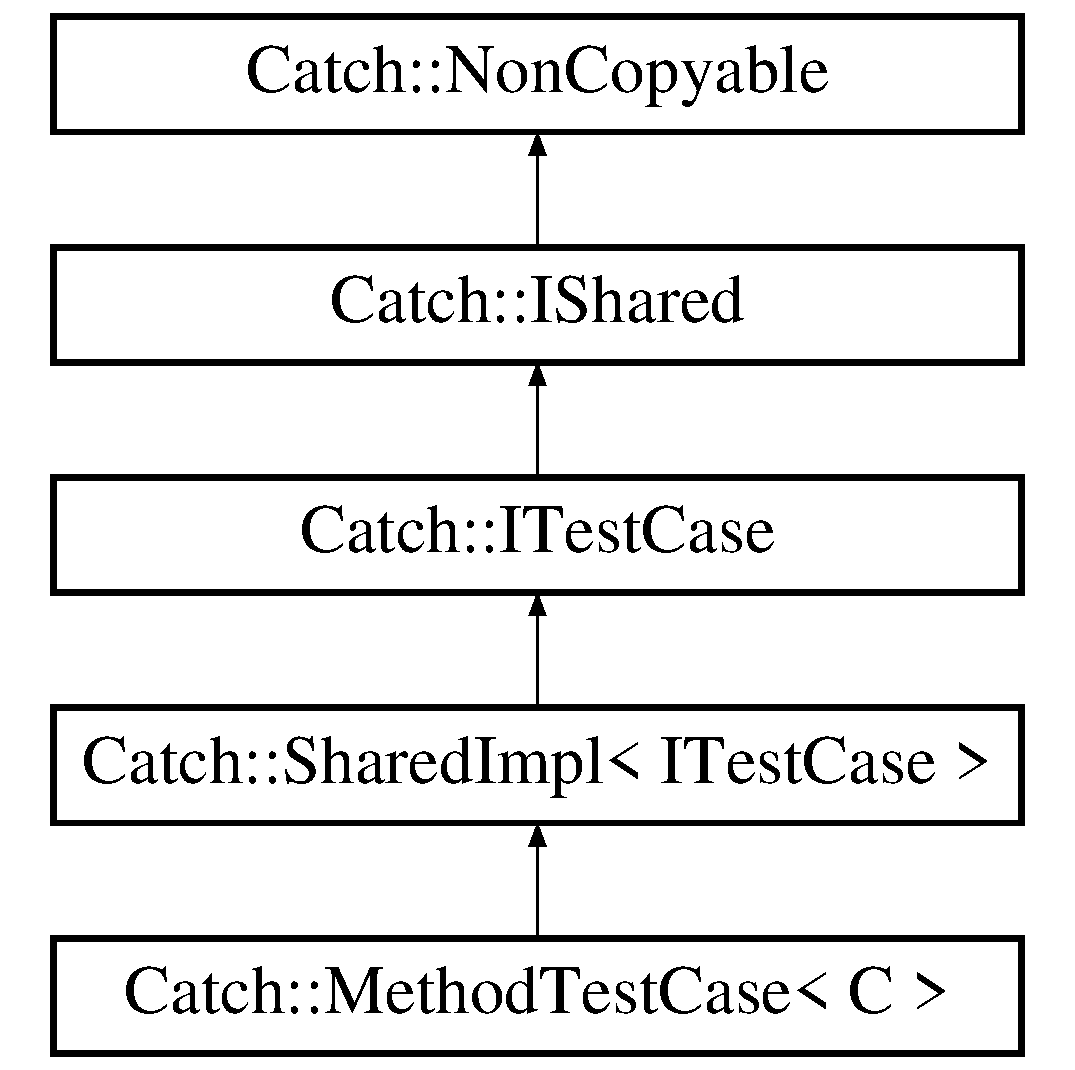
\includegraphics[height=5.000000cm]{structCatch_1_1ITestCase}
\end{center}
\end{figure}
\subsection*{Public Member Functions}
\begin{DoxyCompactItemize}
\item 
virtual void \hyperlink{structCatch_1_1ITestCase_a678825e62e7c17297621cfeb65588c34}{invoke} () const =0
\end{DoxyCompactItemize}
\subsection*{Protected Member Functions}
\begin{DoxyCompactItemize}
\item 
virtual \hyperlink{structCatch_1_1ITestCase_add7b9bec455ac1b007c17df82144310e}{$\sim$\-I\-Test\-Case} ()
\end{DoxyCompactItemize}


\subsection{Constructor \& Destructor Documentation}
\hypertarget{structCatch_1_1ITestCase_add7b9bec455ac1b007c17df82144310e}{\index{Catch\-::\-I\-Test\-Case@{Catch\-::\-I\-Test\-Case}!$\sim$\-I\-Test\-Case@{$\sim$\-I\-Test\-Case}}
\index{$\sim$\-I\-Test\-Case@{$\sim$\-I\-Test\-Case}!Catch::ITestCase@{Catch\-::\-I\-Test\-Case}}
\subsubsection[{$\sim$\-I\-Test\-Case}]{\setlength{\rightskip}{0pt plus 5cm}virtual Catch\-::\-I\-Test\-Case\-::$\sim$\-I\-Test\-Case (
\begin{DoxyParamCaption}
{}
\end{DoxyParamCaption}
)\hspace{0.3cm}{\ttfamily [protected]}, {\ttfamily [virtual]}}}\label{structCatch_1_1ITestCase_add7b9bec455ac1b007c17df82144310e}


\subsection{Member Function Documentation}
\hypertarget{structCatch_1_1ITestCase_a678825e62e7c17297621cfeb65588c34}{\index{Catch\-::\-I\-Test\-Case@{Catch\-::\-I\-Test\-Case}!invoke@{invoke}}
\index{invoke@{invoke}!Catch::ITestCase@{Catch\-::\-I\-Test\-Case}}
\subsubsection[{invoke}]{\setlength{\rightskip}{0pt plus 5cm}virtual void Catch\-::\-I\-Test\-Case\-::invoke (
\begin{DoxyParamCaption}
{}
\end{DoxyParamCaption}
) const\hspace{0.3cm}{\ttfamily [pure virtual]}}}\label{structCatch_1_1ITestCase_a678825e62e7c17297621cfeb65588c34}


Implemented in \hyperlink{classCatch_1_1MethodTestCase_a39cc4b760dd71adc3f7550bc1e7eb697}{Catch\-::\-Method\-Test\-Case$<$ C $>$}.



The documentation for this struct was generated from the following file\-:\begin{DoxyCompactItemize}
\item 
/home/alexander/\-Un\-B/\-M\-P/\-Trabalho\-\_\-2\-\_\-\-M\-P\-\_\-\-Alexander\-\_\-13\-\_\-0039853/include/\hyperlink{catch_8hpp}{catch.\-hpp}\end{DoxyCompactItemize}

\hypertarget{structCatch_1_1ITestCaseRegistry}{\section{Catch\-:\-:I\-Test\-Case\-Registry Struct Reference}
\label{structCatch_1_1ITestCaseRegistry}\index{Catch\-::\-I\-Test\-Case\-Registry@{Catch\-::\-I\-Test\-Case\-Registry}}
}


{\ttfamily \#include $<$catch.\-hpp$>$}

\subsection*{Public Member Functions}
\begin{DoxyCompactItemize}
\item 
virtual \hyperlink{structCatch_1_1ITestCaseRegistry_ae14798f05ac8e2b18cff532849a4da81}{$\sim$\-I\-Test\-Case\-Registry} ()
\item 
virtual std\-::vector$<$ \hyperlink{classCatch_1_1TestCase}{Test\-Case} $>$\\*
 const \& \hyperlink{structCatch_1_1ITestCaseRegistry_ad6e4d4a621655123f73ae98cfeda063d}{get\-All\-Tests} () const =0
\item 
virtual std\-::vector$<$ \hyperlink{classCatch_1_1TestCase}{Test\-Case} $>$\\*
 const \& \hyperlink{structCatch_1_1ITestCaseRegistry_a33e46639d0319d35497c05bb5d02be5a}{get\-All\-Tests\-Sorted} (I\-Config const \&config) const =0
\end{DoxyCompactItemize}


\subsection{Constructor \& Destructor Documentation}
\hypertarget{structCatch_1_1ITestCaseRegistry_ae14798f05ac8e2b18cff532849a4da81}{\index{Catch\-::\-I\-Test\-Case\-Registry@{Catch\-::\-I\-Test\-Case\-Registry}!$\sim$\-I\-Test\-Case\-Registry@{$\sim$\-I\-Test\-Case\-Registry}}
\index{$\sim$\-I\-Test\-Case\-Registry@{$\sim$\-I\-Test\-Case\-Registry}!Catch::ITestCaseRegistry@{Catch\-::\-I\-Test\-Case\-Registry}}
\subsubsection[{$\sim$\-I\-Test\-Case\-Registry}]{\setlength{\rightskip}{0pt plus 5cm}virtual Catch\-::\-I\-Test\-Case\-Registry\-::$\sim$\-I\-Test\-Case\-Registry (
\begin{DoxyParamCaption}
{}
\end{DoxyParamCaption}
)\hspace{0.3cm}{\ttfamily [virtual]}}}\label{structCatch_1_1ITestCaseRegistry_ae14798f05ac8e2b18cff532849a4da81}


\subsection{Member Function Documentation}
\hypertarget{structCatch_1_1ITestCaseRegistry_ad6e4d4a621655123f73ae98cfeda063d}{\index{Catch\-::\-I\-Test\-Case\-Registry@{Catch\-::\-I\-Test\-Case\-Registry}!get\-All\-Tests@{get\-All\-Tests}}
\index{get\-All\-Tests@{get\-All\-Tests}!Catch::ITestCaseRegistry@{Catch\-::\-I\-Test\-Case\-Registry}}
\subsubsection[{get\-All\-Tests}]{\setlength{\rightskip}{0pt plus 5cm}virtual std\-::vector$<${\bf Test\-Case}$>$ const\& Catch\-::\-I\-Test\-Case\-Registry\-::get\-All\-Tests (
\begin{DoxyParamCaption}
{}
\end{DoxyParamCaption}
) const\hspace{0.3cm}{\ttfamily [pure virtual]}}}\label{structCatch_1_1ITestCaseRegistry_ad6e4d4a621655123f73ae98cfeda063d}
\hypertarget{structCatch_1_1ITestCaseRegistry_a33e46639d0319d35497c05bb5d02be5a}{\index{Catch\-::\-I\-Test\-Case\-Registry@{Catch\-::\-I\-Test\-Case\-Registry}!get\-All\-Tests\-Sorted@{get\-All\-Tests\-Sorted}}
\index{get\-All\-Tests\-Sorted@{get\-All\-Tests\-Sorted}!Catch::ITestCaseRegistry@{Catch\-::\-I\-Test\-Case\-Registry}}
\subsubsection[{get\-All\-Tests\-Sorted}]{\setlength{\rightskip}{0pt plus 5cm}virtual std\-::vector$<${\bf Test\-Case}$>$ const\& Catch\-::\-I\-Test\-Case\-Registry\-::get\-All\-Tests\-Sorted (
\begin{DoxyParamCaption}
\item[{I\-Config const \&}]{config}
\end{DoxyParamCaption}
) const\hspace{0.3cm}{\ttfamily [pure virtual]}}}\label{structCatch_1_1ITestCaseRegistry_a33e46639d0319d35497c05bb5d02be5a}


The documentation for this struct was generated from the following file\-:\begin{DoxyCompactItemize}
\item 
/home/alexander/\-Un\-B/\-M\-P/\-Trabalho\-\_\-2\-\_\-\-M\-P\-\_\-\-Alexander\-\_\-13\-\_\-0039853/include/\hyperlink{catch_8hpp}{catch.\-hpp}\end{DoxyCompactItemize}

\hypertarget{structCatch_1_1Matchers_1_1Impl_1_1MatchAllOf}{\section{Catch\-:\-:Matchers\-:\-:Impl\-:\-:Match\-All\-Of$<$ Arg\-T $>$ Struct Template Reference}
\label{structCatch_1_1Matchers_1_1Impl_1_1MatchAllOf}\index{Catch\-::\-Matchers\-::\-Impl\-::\-Match\-All\-Of$<$ Arg\-T $>$@{Catch\-::\-Matchers\-::\-Impl\-::\-Match\-All\-Of$<$ Arg\-T $>$}}
}


{\ttfamily \#include $<$catch.\-hpp$>$}

Inheritance diagram for Catch\-:\-:Matchers\-:\-:Impl\-:\-:Match\-All\-Of$<$ Arg\-T $>$\-:\begin{figure}[H]
\begin{center}
\leavevmode
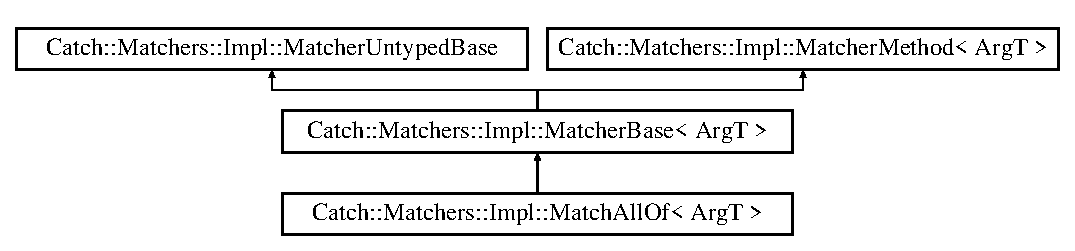
\includegraphics[height=2.926829cm]{structCatch_1_1Matchers_1_1Impl_1_1MatchAllOf}
\end{center}
\end{figure}
\subsection*{Public Member Functions}
\begin{DoxyCompactItemize}
\item 
virtual bool \hyperlink{structCatch_1_1Matchers_1_1Impl_1_1MatchAllOf_a7bf0c2d8cedf67ecf9d0a527cb5a8263}{match} (Arg\-T const \&arg) const \hyperlink{catch_8hpp_a8ecdce4d3f57835f707915ae831eb847}{C\-A\-T\-C\-H\-\_\-\-O\-V\-E\-R\-R\-I\-D\-E}
\item 
virtual std\-::string \hyperlink{structCatch_1_1Matchers_1_1Impl_1_1MatchAllOf_aaefeba99a0b35425203468a65bff544b}{describe} () const \hyperlink{catch_8hpp_a8ecdce4d3f57835f707915ae831eb847}{C\-A\-T\-C\-H\-\_\-\-O\-V\-E\-R\-R\-I\-D\-E}
\item 
\hyperlink{structCatch_1_1Matchers_1_1Impl_1_1MatchAllOf}{Match\-All\-Of}$<$ Arg\-T $>$ \& \hyperlink{structCatch_1_1Matchers_1_1Impl_1_1MatchAllOf_a3844f9fb55f7a77155576ddc1e3f90d7}{operator\&\&} (\hyperlink{structCatch_1_1Matchers_1_1Impl_1_1MatcherBase}{Matcher\-Base}$<$ Arg\-T $>$ const \&other)
\end{DoxyCompactItemize}
\subsection*{Public Attributes}
\begin{DoxyCompactItemize}
\item 
std\-::vector$<$ \hyperlink{structCatch_1_1Matchers_1_1Impl_1_1MatcherBase}{Matcher\-Base}$<$ Arg\-T $>$\\*
 const $\ast$ $>$ \hyperlink{structCatch_1_1Matchers_1_1Impl_1_1MatchAllOf_a98d6a2611f195a4a5c49f92fd877be9a}{m\-\_\-matchers}
\end{DoxyCompactItemize}
\subsection*{Additional Inherited Members}


\subsection{Member Function Documentation}
\hypertarget{structCatch_1_1Matchers_1_1Impl_1_1MatchAllOf_aaefeba99a0b35425203468a65bff544b}{\index{Catch\-::\-Matchers\-::\-Impl\-::\-Match\-All\-Of@{Catch\-::\-Matchers\-::\-Impl\-::\-Match\-All\-Of}!describe@{describe}}
\index{describe@{describe}!Catch::Matchers::Impl::MatchAllOf@{Catch\-::\-Matchers\-::\-Impl\-::\-Match\-All\-Of}}
\subsubsection[{describe}]{\setlength{\rightskip}{0pt plus 5cm}template$<$typename Arg\-T$>$ virtual std\-::string {\bf Catch\-::\-Matchers\-::\-Impl\-::\-Match\-All\-Of}$<$ Arg\-T $>$\-::describe (
\begin{DoxyParamCaption}
{}
\end{DoxyParamCaption}
) const\hspace{0.3cm}{\ttfamily [inline]}, {\ttfamily [virtual]}}}\label{structCatch_1_1Matchers_1_1Impl_1_1MatchAllOf_aaefeba99a0b35425203468a65bff544b}


Implements \hyperlink{classCatch_1_1Matchers_1_1Impl_1_1MatcherUntypedBase_a91d3a907dbfcbb596077df24f6e11fe2}{Catch\-::\-Matchers\-::\-Impl\-::\-Matcher\-Untyped\-Base}.

\hypertarget{structCatch_1_1Matchers_1_1Impl_1_1MatchAllOf_a7bf0c2d8cedf67ecf9d0a527cb5a8263}{\index{Catch\-::\-Matchers\-::\-Impl\-::\-Match\-All\-Of@{Catch\-::\-Matchers\-::\-Impl\-::\-Match\-All\-Of}!match@{match}}
\index{match@{match}!Catch::Matchers::Impl::MatchAllOf@{Catch\-::\-Matchers\-::\-Impl\-::\-Match\-All\-Of}}
\subsubsection[{match}]{\setlength{\rightskip}{0pt plus 5cm}template$<$typename Arg\-T$>$ virtual bool {\bf Catch\-::\-Matchers\-::\-Impl\-::\-Match\-All\-Of}$<$ Arg\-T $>$\-::match (
\begin{DoxyParamCaption}
\item[{Arg\-T const \&}]{arg}
\end{DoxyParamCaption}
) const\hspace{0.3cm}{\ttfamily [inline]}, {\ttfamily [virtual]}}}\label{structCatch_1_1Matchers_1_1Impl_1_1MatchAllOf_a7bf0c2d8cedf67ecf9d0a527cb5a8263}


Implements \hyperlink{structCatch_1_1Matchers_1_1Impl_1_1MatcherMethod_ae0920ff9e817acf08e1bb0cbcb044e30}{Catch\-::\-Matchers\-::\-Impl\-::\-Matcher\-Method$<$ Arg\-T $>$}.

\hypertarget{structCatch_1_1Matchers_1_1Impl_1_1MatchAllOf_a3844f9fb55f7a77155576ddc1e3f90d7}{\index{Catch\-::\-Matchers\-::\-Impl\-::\-Match\-All\-Of@{Catch\-::\-Matchers\-::\-Impl\-::\-Match\-All\-Of}!operator\&\&@{operator\&\&}}
\index{operator\&\&@{operator\&\&}!Catch::Matchers::Impl::MatchAllOf@{Catch\-::\-Matchers\-::\-Impl\-::\-Match\-All\-Of}}
\subsubsection[{operator\&\&}]{\setlength{\rightskip}{0pt plus 5cm}template$<$typename Arg\-T$>$ {\bf Match\-All\-Of}$<$Arg\-T$>$\& {\bf Catch\-::\-Matchers\-::\-Impl\-::\-Match\-All\-Of}$<$ Arg\-T $>$\-::operator\&\& (
\begin{DoxyParamCaption}
\item[{{\bf Matcher\-Base}$<$ Arg\-T $>$ const \&}]{other}
\end{DoxyParamCaption}
)\hspace{0.3cm}{\ttfamily [inline]}}}\label{structCatch_1_1Matchers_1_1Impl_1_1MatchAllOf_a3844f9fb55f7a77155576ddc1e3f90d7}


\subsection{Member Data Documentation}
\hypertarget{structCatch_1_1Matchers_1_1Impl_1_1MatchAllOf_a98d6a2611f195a4a5c49f92fd877be9a}{\index{Catch\-::\-Matchers\-::\-Impl\-::\-Match\-All\-Of@{Catch\-::\-Matchers\-::\-Impl\-::\-Match\-All\-Of}!m\-\_\-matchers@{m\-\_\-matchers}}
\index{m\-\_\-matchers@{m\-\_\-matchers}!Catch::Matchers::Impl::MatchAllOf@{Catch\-::\-Matchers\-::\-Impl\-::\-Match\-All\-Of}}
\subsubsection[{m\-\_\-matchers}]{\setlength{\rightskip}{0pt plus 5cm}template$<$typename Arg\-T$>$ std\-::vector$<${\bf Matcher\-Base}$<$Arg\-T$>$ const$\ast$$>$ {\bf Catch\-::\-Matchers\-::\-Impl\-::\-Match\-All\-Of}$<$ Arg\-T $>$\-::m\-\_\-matchers}}\label{structCatch_1_1Matchers_1_1Impl_1_1MatchAllOf_a98d6a2611f195a4a5c49f92fd877be9a}


The documentation for this struct was generated from the following file\-:\begin{DoxyCompactItemize}
\item 
/home/alexander/\-Un\-B/\-M\-P/\-Trabalho\-\_\-2\-\_\-\-M\-P\-\_\-\-Alexander\-\_\-13\-\_\-0039853/include/\hyperlink{catch_8hpp}{catch.\-hpp}\end{DoxyCompactItemize}

\hypertarget{structCatch_1_1Matchers_1_1Impl_1_1MatchAnyOf}{\section{Catch\-:\-:Matchers\-:\-:Impl\-:\-:Match\-Any\-Of$<$ Arg\-T $>$ Struct Template Reference}
\label{structCatch_1_1Matchers_1_1Impl_1_1MatchAnyOf}\index{Catch\-::\-Matchers\-::\-Impl\-::\-Match\-Any\-Of$<$ Arg\-T $>$@{Catch\-::\-Matchers\-::\-Impl\-::\-Match\-Any\-Of$<$ Arg\-T $>$}}
}


{\ttfamily \#include $<$catch.\-hpp$>$}

Inheritance diagram for Catch\-:\-:Matchers\-:\-:Impl\-:\-:Match\-Any\-Of$<$ Arg\-T $>$\-:\begin{figure}[H]
\begin{center}
\leavevmode
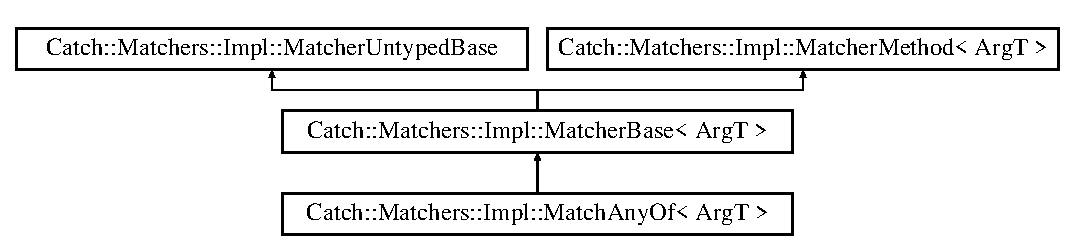
\includegraphics[height=2.926829cm]{structCatch_1_1Matchers_1_1Impl_1_1MatchAnyOf}
\end{center}
\end{figure}
\subsection*{Public Member Functions}
\begin{DoxyCompactItemize}
\item 
virtual bool \hyperlink{structCatch_1_1Matchers_1_1Impl_1_1MatchAnyOf_a73be317ecf5919af855af96d68e714b9}{match} (Arg\-T const \&arg) const \hyperlink{catch_8hpp_a8ecdce4d3f57835f707915ae831eb847}{C\-A\-T\-C\-H\-\_\-\-O\-V\-E\-R\-R\-I\-D\-E}
\item 
virtual std\-::string \hyperlink{structCatch_1_1Matchers_1_1Impl_1_1MatchAnyOf_a020f5d7889d8cd8be9ad309c690147b6}{describe} () const \hyperlink{catch_8hpp_a8ecdce4d3f57835f707915ae831eb847}{C\-A\-T\-C\-H\-\_\-\-O\-V\-E\-R\-R\-I\-D\-E}
\item 
\hyperlink{structCatch_1_1Matchers_1_1Impl_1_1MatchAnyOf}{Match\-Any\-Of}$<$ Arg\-T $>$ \& \hyperlink{structCatch_1_1Matchers_1_1Impl_1_1MatchAnyOf_a44d7582dbe09fc31b9a5ba8a6367b506}{operator$\vert$$\vert$} (\hyperlink{structCatch_1_1Matchers_1_1Impl_1_1MatcherBase}{Matcher\-Base}$<$ Arg\-T $>$ const \&other)
\end{DoxyCompactItemize}
\subsection*{Public Attributes}
\begin{DoxyCompactItemize}
\item 
std\-::vector$<$ \hyperlink{structCatch_1_1Matchers_1_1Impl_1_1MatcherBase}{Matcher\-Base}$<$ Arg\-T $>$\\*
 const $\ast$ $>$ \hyperlink{structCatch_1_1Matchers_1_1Impl_1_1MatchAnyOf_a1fb1119e6110dc15b8d5262ec0aeddd5}{m\-\_\-matchers}
\end{DoxyCompactItemize}
\subsection*{Additional Inherited Members}


\subsection{Member Function Documentation}
\hypertarget{structCatch_1_1Matchers_1_1Impl_1_1MatchAnyOf_a020f5d7889d8cd8be9ad309c690147b6}{\index{Catch\-::\-Matchers\-::\-Impl\-::\-Match\-Any\-Of@{Catch\-::\-Matchers\-::\-Impl\-::\-Match\-Any\-Of}!describe@{describe}}
\index{describe@{describe}!Catch::Matchers::Impl::MatchAnyOf@{Catch\-::\-Matchers\-::\-Impl\-::\-Match\-Any\-Of}}
\subsubsection[{describe}]{\setlength{\rightskip}{0pt plus 5cm}template$<$typename Arg\-T$>$ virtual std\-::string {\bf Catch\-::\-Matchers\-::\-Impl\-::\-Match\-Any\-Of}$<$ Arg\-T $>$\-::describe (
\begin{DoxyParamCaption}
{}
\end{DoxyParamCaption}
) const\hspace{0.3cm}{\ttfamily [inline]}, {\ttfamily [virtual]}}}\label{structCatch_1_1Matchers_1_1Impl_1_1MatchAnyOf_a020f5d7889d8cd8be9ad309c690147b6}


Implements \hyperlink{classCatch_1_1Matchers_1_1Impl_1_1MatcherUntypedBase_a91d3a907dbfcbb596077df24f6e11fe2}{Catch\-::\-Matchers\-::\-Impl\-::\-Matcher\-Untyped\-Base}.

\hypertarget{structCatch_1_1Matchers_1_1Impl_1_1MatchAnyOf_a73be317ecf5919af855af96d68e714b9}{\index{Catch\-::\-Matchers\-::\-Impl\-::\-Match\-Any\-Of@{Catch\-::\-Matchers\-::\-Impl\-::\-Match\-Any\-Of}!match@{match}}
\index{match@{match}!Catch::Matchers::Impl::MatchAnyOf@{Catch\-::\-Matchers\-::\-Impl\-::\-Match\-Any\-Of}}
\subsubsection[{match}]{\setlength{\rightskip}{0pt plus 5cm}template$<$typename Arg\-T$>$ virtual bool {\bf Catch\-::\-Matchers\-::\-Impl\-::\-Match\-Any\-Of}$<$ Arg\-T $>$\-::match (
\begin{DoxyParamCaption}
\item[{Arg\-T const \&}]{arg}
\end{DoxyParamCaption}
) const\hspace{0.3cm}{\ttfamily [inline]}, {\ttfamily [virtual]}}}\label{structCatch_1_1Matchers_1_1Impl_1_1MatchAnyOf_a73be317ecf5919af855af96d68e714b9}


Implements \hyperlink{structCatch_1_1Matchers_1_1Impl_1_1MatcherMethod_ae0920ff9e817acf08e1bb0cbcb044e30}{Catch\-::\-Matchers\-::\-Impl\-::\-Matcher\-Method$<$ Arg\-T $>$}.

\hypertarget{structCatch_1_1Matchers_1_1Impl_1_1MatchAnyOf_a44d7582dbe09fc31b9a5ba8a6367b506}{\index{Catch\-::\-Matchers\-::\-Impl\-::\-Match\-Any\-Of@{Catch\-::\-Matchers\-::\-Impl\-::\-Match\-Any\-Of}!operator$\vert$$\vert$@{operator$\vert$$\vert$}}
\index{operator$\vert$$\vert$@{operator$\vert$$\vert$}!Catch::Matchers::Impl::MatchAnyOf@{Catch\-::\-Matchers\-::\-Impl\-::\-Match\-Any\-Of}}
\subsubsection[{operator$\vert$$\vert$}]{\setlength{\rightskip}{0pt plus 5cm}template$<$typename Arg\-T$>$ {\bf Match\-Any\-Of}$<$Arg\-T$>$\& {\bf Catch\-::\-Matchers\-::\-Impl\-::\-Match\-Any\-Of}$<$ Arg\-T $>$\-::operator$\vert$$\vert$ (
\begin{DoxyParamCaption}
\item[{{\bf Matcher\-Base}$<$ Arg\-T $>$ const \&}]{other}
\end{DoxyParamCaption}
)\hspace{0.3cm}{\ttfamily [inline]}}}\label{structCatch_1_1Matchers_1_1Impl_1_1MatchAnyOf_a44d7582dbe09fc31b9a5ba8a6367b506}


\subsection{Member Data Documentation}
\hypertarget{structCatch_1_1Matchers_1_1Impl_1_1MatchAnyOf_a1fb1119e6110dc15b8d5262ec0aeddd5}{\index{Catch\-::\-Matchers\-::\-Impl\-::\-Match\-Any\-Of@{Catch\-::\-Matchers\-::\-Impl\-::\-Match\-Any\-Of}!m\-\_\-matchers@{m\-\_\-matchers}}
\index{m\-\_\-matchers@{m\-\_\-matchers}!Catch::Matchers::Impl::MatchAnyOf@{Catch\-::\-Matchers\-::\-Impl\-::\-Match\-Any\-Of}}
\subsubsection[{m\-\_\-matchers}]{\setlength{\rightskip}{0pt plus 5cm}template$<$typename Arg\-T$>$ std\-::vector$<${\bf Matcher\-Base}$<$Arg\-T$>$ const$\ast$$>$ {\bf Catch\-::\-Matchers\-::\-Impl\-::\-Match\-Any\-Of}$<$ Arg\-T $>$\-::m\-\_\-matchers}}\label{structCatch_1_1Matchers_1_1Impl_1_1MatchAnyOf_a1fb1119e6110dc15b8d5262ec0aeddd5}


The documentation for this struct was generated from the following file\-:\begin{DoxyCompactItemize}
\item 
/home/alexander/\-Un\-B/\-M\-P/\-Trabalho\-\_\-2\-\_\-\-M\-P\-\_\-\-Alexander\-\_\-13\-\_\-0039853/include/\hyperlink{catch_8hpp}{catch.\-hpp}\end{DoxyCompactItemize}

\hypertarget{structCatch_1_1Matchers_1_1Impl_1_1MatcherBase}{\section{Catch\-:\-:Matchers\-:\-:Impl\-:\-:Matcher\-Base$<$ Object\-T, Comparator\-T $>$ Struct Template Reference}
\label{structCatch_1_1Matchers_1_1Impl_1_1MatcherBase}\index{Catch\-::\-Matchers\-::\-Impl\-::\-Matcher\-Base$<$ Object\-T, Comparator\-T $>$@{Catch\-::\-Matchers\-::\-Impl\-::\-Matcher\-Base$<$ Object\-T, Comparator\-T $>$}}
}


{\ttfamily \#include $<$catch.\-hpp$>$}

Inheritance diagram for Catch\-:\-:Matchers\-:\-:Impl\-:\-:Matcher\-Base$<$ Object\-T, Comparator\-T $>$\-:\begin{figure}[H]
\begin{center}
\leavevmode
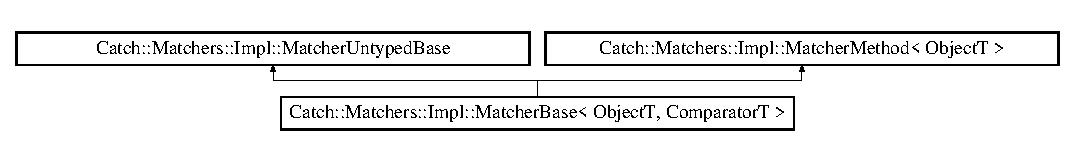
\includegraphics[height=1.509434cm]{structCatch_1_1Matchers_1_1Impl_1_1MatcherBase}
\end{center}
\end{figure}
\subsection*{Public Member Functions}
\begin{DoxyCompactItemize}
\item 
\hyperlink{structCatch_1_1Matchers_1_1Impl_1_1MatchAllOf}{Match\-All\-Of}$<$ Comparator\-T $>$ \hyperlink{structCatch_1_1Matchers_1_1Impl_1_1MatcherBase_a0a81a1cf1955daf438fba5607e036e56}{operator\&\&} (\hyperlink{structCatch_1_1Matchers_1_1Impl_1_1MatcherBase}{Matcher\-Base} const \&other) const 
\item 
\hyperlink{structCatch_1_1Matchers_1_1Impl_1_1MatchAnyOf}{Match\-Any\-Of}$<$ Comparator\-T $>$ \hyperlink{structCatch_1_1Matchers_1_1Impl_1_1MatcherBase_a5241c16329b71ce181c3f3fd599d6e06}{operator$\vert$$\vert$} (\hyperlink{structCatch_1_1Matchers_1_1Impl_1_1MatcherBase}{Matcher\-Base} const \&other) const 
\item 
\hyperlink{structCatch_1_1Matchers_1_1Impl_1_1MatchNotOf}{Match\-Not\-Of}$<$ Comparator\-T $>$ \hyperlink{structCatch_1_1Matchers_1_1Impl_1_1MatcherBase_a1c40d784bc484b968bdda10b076709c2}{operator!} () const 
\end{DoxyCompactItemize}
\subsection*{Additional Inherited Members}


\subsection{Member Function Documentation}
\hypertarget{structCatch_1_1Matchers_1_1Impl_1_1MatcherBase_a1c40d784bc484b968bdda10b076709c2}{\index{Catch\-::\-Matchers\-::\-Impl\-::\-Matcher\-Base@{Catch\-::\-Matchers\-::\-Impl\-::\-Matcher\-Base}!operator!@{operator!}}
\index{operator!@{operator!}!Catch::Matchers::Impl::MatcherBase@{Catch\-::\-Matchers\-::\-Impl\-::\-Matcher\-Base}}
\subsubsection[{operator!}]{\setlength{\rightskip}{0pt plus 5cm}template$<$typename Object\-T , typename Comparator\-T $>$ {\bf Match\-Not\-Of}$<$ Comparator\-T $>$ {\bf Catch\-::\-Matchers\-::\-Impl\-::\-Matcher\-Base}$<$ Object\-T, Comparator\-T $>$\-::operator! (
\begin{DoxyParamCaption}
{}
\end{DoxyParamCaption}
) const}}\label{structCatch_1_1Matchers_1_1Impl_1_1MatcherBase_a1c40d784bc484b968bdda10b076709c2}
\hypertarget{structCatch_1_1Matchers_1_1Impl_1_1MatcherBase_a0a81a1cf1955daf438fba5607e036e56}{\index{Catch\-::\-Matchers\-::\-Impl\-::\-Matcher\-Base@{Catch\-::\-Matchers\-::\-Impl\-::\-Matcher\-Base}!operator\&\&@{operator\&\&}}
\index{operator\&\&@{operator\&\&}!Catch::Matchers::Impl::MatcherBase@{Catch\-::\-Matchers\-::\-Impl\-::\-Matcher\-Base}}
\subsubsection[{operator\&\&}]{\setlength{\rightskip}{0pt plus 5cm}template$<$typename Object\-T , typename Comparator\-T $>$ {\bf Match\-All\-Of}$<$ Comparator\-T $>$ {\bf Catch\-::\-Matchers\-::\-Impl\-::\-Matcher\-Base}$<$ Object\-T, Comparator\-T $>$\-::operator\&\& (
\begin{DoxyParamCaption}
\item[{{\bf Matcher\-Base}$<$ Object\-T, Comparator\-T $>$ const \&}]{other}
\end{DoxyParamCaption}
) const}}\label{structCatch_1_1Matchers_1_1Impl_1_1MatcherBase_a0a81a1cf1955daf438fba5607e036e56}
\hypertarget{structCatch_1_1Matchers_1_1Impl_1_1MatcherBase_a5241c16329b71ce181c3f3fd599d6e06}{\index{Catch\-::\-Matchers\-::\-Impl\-::\-Matcher\-Base@{Catch\-::\-Matchers\-::\-Impl\-::\-Matcher\-Base}!operator$\vert$$\vert$@{operator$\vert$$\vert$}}
\index{operator$\vert$$\vert$@{operator$\vert$$\vert$}!Catch::Matchers::Impl::MatcherBase@{Catch\-::\-Matchers\-::\-Impl\-::\-Matcher\-Base}}
\subsubsection[{operator$\vert$$\vert$}]{\setlength{\rightskip}{0pt plus 5cm}template$<$typename Object\-T , typename Comparator\-T $>$ {\bf Match\-Any\-Of}$<$ Comparator\-T $>$ {\bf Catch\-::\-Matchers\-::\-Impl\-::\-Matcher\-Base}$<$ Object\-T, Comparator\-T $>$\-::operator$\vert$$\vert$ (
\begin{DoxyParamCaption}
\item[{{\bf Matcher\-Base}$<$ Object\-T, Comparator\-T $>$ const \&}]{other}
\end{DoxyParamCaption}
) const}}\label{structCatch_1_1Matchers_1_1Impl_1_1MatcherBase_a5241c16329b71ce181c3f3fd599d6e06}


The documentation for this struct was generated from the following file\-:\begin{DoxyCompactItemize}
\item 
/home/alexander/\-Un\-B/\-M\-P/\-Trabalho\-\_\-2\-\_\-\-M\-P\-\_\-\-Alexander\-\_\-13\-\_\-0039853/include/\hyperlink{catch_8hpp}{catch.\-hpp}\end{DoxyCompactItemize}

\hypertarget{structCatch_1_1Matchers_1_1Impl_1_1MatcherMethod}{\section{Catch\-:\-:Matchers\-:\-:Impl\-:\-:Matcher\-Method$<$ Object\-T $>$ Struct Template Reference}
\label{structCatch_1_1Matchers_1_1Impl_1_1MatcherMethod}\index{Catch\-::\-Matchers\-::\-Impl\-::\-Matcher\-Method$<$ Object\-T $>$@{Catch\-::\-Matchers\-::\-Impl\-::\-Matcher\-Method$<$ Object\-T $>$}}
}


{\ttfamily \#include $<$catch.\-hpp$>$}

Inheritance diagram for Catch\-:\-:Matchers\-:\-:Impl\-:\-:Matcher\-Method$<$ Object\-T $>$\-:\begin{figure}[H]
\begin{center}
\leavevmode
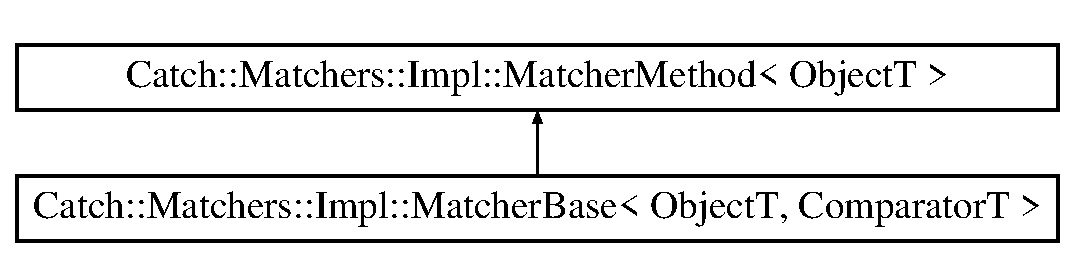
\includegraphics[height=2.000000cm]{structCatch_1_1Matchers_1_1Impl_1_1MatcherMethod}
\end{center}
\end{figure}
\subsection*{Public Member Functions}
\begin{DoxyCompactItemize}
\item 
virtual bool \hyperlink{structCatch_1_1Matchers_1_1Impl_1_1MatcherMethod_ae0920ff9e817acf08e1bb0cbcb044e30}{match} (Object\-T const \&arg) const =0
\end{DoxyCompactItemize}


\subsection{Member Function Documentation}
\hypertarget{structCatch_1_1Matchers_1_1Impl_1_1MatcherMethod_ae0920ff9e817acf08e1bb0cbcb044e30}{\index{Catch\-::\-Matchers\-::\-Impl\-::\-Matcher\-Method@{Catch\-::\-Matchers\-::\-Impl\-::\-Matcher\-Method}!match@{match}}
\index{match@{match}!Catch::Matchers::Impl::MatcherMethod@{Catch\-::\-Matchers\-::\-Impl\-::\-Matcher\-Method}}
\subsubsection[{match}]{\setlength{\rightskip}{0pt plus 5cm}template$<$typename Object\-T$>$ virtual bool {\bf Catch\-::\-Matchers\-::\-Impl\-::\-Matcher\-Method}$<$ Object\-T $>$\-::match (
\begin{DoxyParamCaption}
\item[{Object\-T const \&}]{arg}
\end{DoxyParamCaption}
) const\hspace{0.3cm}{\ttfamily [pure virtual]}}}\label{structCatch_1_1Matchers_1_1Impl_1_1MatcherMethod_ae0920ff9e817acf08e1bb0cbcb044e30}


Implemented in \hyperlink{structCatch_1_1Matchers_1_1Impl_1_1MatchNotOf_a1b9ad6566e4ab0f292d2903f557307cc}{Catch\-::\-Matchers\-::\-Impl\-::\-Match\-Not\-Of$<$ Arg\-T $>$}, \hyperlink{structCatch_1_1Matchers_1_1Impl_1_1MatchAnyOf_a73be317ecf5919af855af96d68e714b9}{Catch\-::\-Matchers\-::\-Impl\-::\-Match\-Any\-Of$<$ Arg\-T $>$}, and \hyperlink{structCatch_1_1Matchers_1_1Impl_1_1MatchAllOf_a7bf0c2d8cedf67ecf9d0a527cb5a8263}{Catch\-::\-Matchers\-::\-Impl\-::\-Match\-All\-Of$<$ Arg\-T $>$}.



The documentation for this struct was generated from the following file\-:\begin{DoxyCompactItemize}
\item 
/home/alexander/\-Un\-B/\-M\-P/\-Trabalho\-\_\-2\-\_\-\-M\-P\-\_\-\-Alexander\-\_\-13\-\_\-0039853/include/\hyperlink{catch_8hpp}{catch.\-hpp}\end{DoxyCompactItemize}

\hypertarget{structCatch_1_1Matchers_1_1Impl_1_1MatcherMethod_3_01PtrT_01_5_01_4}{\section{Catch\-:\-:Matchers\-:\-:Impl\-:\-:Matcher\-Method$<$ Ptr\-T $\ast$ $>$ Struct Template Reference}
\label{structCatch_1_1Matchers_1_1Impl_1_1MatcherMethod_3_01PtrT_01_5_01_4}\index{Catch\-::\-Matchers\-::\-Impl\-::\-Matcher\-Method$<$ Ptr\-T $\ast$ $>$@{Catch\-::\-Matchers\-::\-Impl\-::\-Matcher\-Method$<$ Ptr\-T $\ast$ $>$}}
}


{\ttfamily \#include $<$catch.\-hpp$>$}

\subsection*{Public Member Functions}
\begin{DoxyCompactItemize}
\item 
virtual bool \hyperlink{structCatch_1_1Matchers_1_1Impl_1_1MatcherMethod_3_01PtrT_01_5_01_4_a5fdd64f9509724f32ffc73cb320181d1}{match} (Ptr\-T $\ast$arg) const =0
\end{DoxyCompactItemize}


\subsection{Member Function Documentation}
\hypertarget{structCatch_1_1Matchers_1_1Impl_1_1MatcherMethod_3_01PtrT_01_5_01_4_a5fdd64f9509724f32ffc73cb320181d1}{\index{Catch\-::\-Matchers\-::\-Impl\-::\-Matcher\-Method$<$ Ptr\-T $\ast$ $>$@{Catch\-::\-Matchers\-::\-Impl\-::\-Matcher\-Method$<$ Ptr\-T $\ast$ $>$}!match@{match}}
\index{match@{match}!Catch::Matchers::Impl::MatcherMethod< PtrT * >@{Catch\-::\-Matchers\-::\-Impl\-::\-Matcher\-Method$<$ Ptr\-T $\ast$ $>$}}
\subsubsection[{match}]{\setlength{\rightskip}{0pt plus 5cm}template$<$typename Ptr\-T $>$ virtual bool {\bf Catch\-::\-Matchers\-::\-Impl\-::\-Matcher\-Method}$<$ Ptr\-T $\ast$ $>$\-::match (
\begin{DoxyParamCaption}
\item[{Ptr\-T $\ast$}]{arg}
\end{DoxyParamCaption}
) const\hspace{0.3cm}{\ttfamily [pure virtual]}}}\label{structCatch_1_1Matchers_1_1Impl_1_1MatcherMethod_3_01PtrT_01_5_01_4_a5fdd64f9509724f32ffc73cb320181d1}


The documentation for this struct was generated from the following file\-:\begin{DoxyCompactItemize}
\item 
/home/alexander/\-Un\-B/\-M\-P/\-Trabalho\-\_\-2\-\_\-\-M\-P\-\_\-\-Alexander\-\_\-13\-\_\-0039853/include/\hyperlink{catch_8hpp}{catch.\-hpp}\end{DoxyCompactItemize}

\hypertarget{classCatch_1_1Matchers_1_1Impl_1_1MatcherUntypedBase}{\section{Catch\-:\-:Matchers\-:\-:Impl\-:\-:Matcher\-Untyped\-Base Class Reference}
\label{classCatch_1_1Matchers_1_1Impl_1_1MatcherUntypedBase}\index{Catch\-::\-Matchers\-::\-Impl\-::\-Matcher\-Untyped\-Base@{Catch\-::\-Matchers\-::\-Impl\-::\-Matcher\-Untyped\-Base}}
}


{\ttfamily \#include $<$catch.\-hpp$>$}

Inheritance diagram for Catch\-:\-:Matchers\-:\-:Impl\-:\-:Matcher\-Untyped\-Base\-:\begin{figure}[H]
\begin{center}
\leavevmode
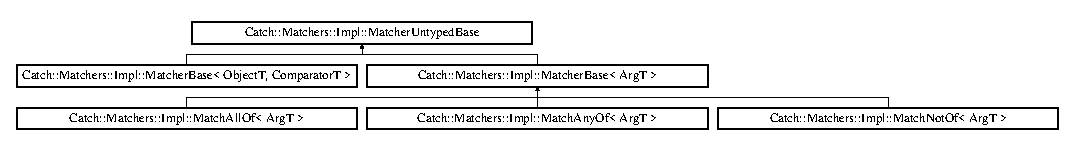
\includegraphics[height=1.509434cm]{classCatch_1_1Matchers_1_1Impl_1_1MatcherUntypedBase}
\end{center}
\end{figure}
\subsection*{Public Member Functions}
\begin{DoxyCompactItemize}
\item 
std\-::string \hyperlink{classCatch_1_1Matchers_1_1Impl_1_1MatcherUntypedBase_a9667f989b08e52a1ce96c955456db8f9}{to\-String} () const 
\end{DoxyCompactItemize}
\subsection*{Protected Member Functions}
\begin{DoxyCompactItemize}
\item 
virtual \hyperlink{classCatch_1_1Matchers_1_1Impl_1_1MatcherUntypedBase_a853be93ce33f71b5abede38081c79e9d}{$\sim$\-Matcher\-Untyped\-Base} ()
\item 
virtual std\-::string \hyperlink{classCatch_1_1Matchers_1_1Impl_1_1MatcherUntypedBase_a91d3a907dbfcbb596077df24f6e11fe2}{describe} () const =0
\end{DoxyCompactItemize}
\subsection*{Protected Attributes}
\begin{DoxyCompactItemize}
\item 
std\-::string \hyperlink{classCatch_1_1Matchers_1_1Impl_1_1MatcherUntypedBase_a951095c462657e7097a9a6dc4dde813f}{m\-\_\-cached\-To\-String}
\end{DoxyCompactItemize}


\subsection{Constructor \& Destructor Documentation}
\hypertarget{classCatch_1_1Matchers_1_1Impl_1_1MatcherUntypedBase_a853be93ce33f71b5abede38081c79e9d}{\index{Catch\-::\-Matchers\-::\-Impl\-::\-Matcher\-Untyped\-Base@{Catch\-::\-Matchers\-::\-Impl\-::\-Matcher\-Untyped\-Base}!$\sim$\-Matcher\-Untyped\-Base@{$\sim$\-Matcher\-Untyped\-Base}}
\index{$\sim$\-Matcher\-Untyped\-Base@{$\sim$\-Matcher\-Untyped\-Base}!Catch::Matchers::Impl::MatcherUntypedBase@{Catch\-::\-Matchers\-::\-Impl\-::\-Matcher\-Untyped\-Base}}
\subsubsection[{$\sim$\-Matcher\-Untyped\-Base}]{\setlength{\rightskip}{0pt plus 5cm}virtual Catch\-::\-Matchers\-::\-Impl\-::\-Matcher\-Untyped\-Base\-::$\sim$\-Matcher\-Untyped\-Base (
\begin{DoxyParamCaption}
{}
\end{DoxyParamCaption}
)\hspace{0.3cm}{\ttfamily [protected]}, {\ttfamily [virtual]}}}\label{classCatch_1_1Matchers_1_1Impl_1_1MatcherUntypedBase_a853be93ce33f71b5abede38081c79e9d}


\subsection{Member Function Documentation}
\hypertarget{classCatch_1_1Matchers_1_1Impl_1_1MatcherUntypedBase_a91d3a907dbfcbb596077df24f6e11fe2}{\index{Catch\-::\-Matchers\-::\-Impl\-::\-Matcher\-Untyped\-Base@{Catch\-::\-Matchers\-::\-Impl\-::\-Matcher\-Untyped\-Base}!describe@{describe}}
\index{describe@{describe}!Catch::Matchers::Impl::MatcherUntypedBase@{Catch\-::\-Matchers\-::\-Impl\-::\-Matcher\-Untyped\-Base}}
\subsubsection[{describe}]{\setlength{\rightskip}{0pt plus 5cm}virtual std\-::string Catch\-::\-Matchers\-::\-Impl\-::\-Matcher\-Untyped\-Base\-::describe (
\begin{DoxyParamCaption}
{}
\end{DoxyParamCaption}
) const\hspace{0.3cm}{\ttfamily [protected]}, {\ttfamily [pure virtual]}}}\label{classCatch_1_1Matchers_1_1Impl_1_1MatcherUntypedBase_a91d3a907dbfcbb596077df24f6e11fe2}


Implemented in \hyperlink{structCatch_1_1Matchers_1_1Impl_1_1MatchNotOf_a62bdc7dcb9ff000438a4ed3d5483a248}{Catch\-::\-Matchers\-::\-Impl\-::\-Match\-Not\-Of$<$ Arg\-T $>$}, \hyperlink{structCatch_1_1Matchers_1_1Impl_1_1MatchAnyOf_a020f5d7889d8cd8be9ad309c690147b6}{Catch\-::\-Matchers\-::\-Impl\-::\-Match\-Any\-Of$<$ Arg\-T $>$}, and \hyperlink{structCatch_1_1Matchers_1_1Impl_1_1MatchAllOf_aaefeba99a0b35425203468a65bff544b}{Catch\-::\-Matchers\-::\-Impl\-::\-Match\-All\-Of$<$ Arg\-T $>$}.

\hypertarget{classCatch_1_1Matchers_1_1Impl_1_1MatcherUntypedBase_a9667f989b08e52a1ce96c955456db8f9}{\index{Catch\-::\-Matchers\-::\-Impl\-::\-Matcher\-Untyped\-Base@{Catch\-::\-Matchers\-::\-Impl\-::\-Matcher\-Untyped\-Base}!to\-String@{to\-String}}
\index{to\-String@{to\-String}!Catch::Matchers::Impl::MatcherUntypedBase@{Catch\-::\-Matchers\-::\-Impl\-::\-Matcher\-Untyped\-Base}}
\subsubsection[{to\-String}]{\setlength{\rightskip}{0pt plus 5cm}std\-::string Catch\-::\-Matchers\-::\-Impl\-::\-Matcher\-Untyped\-Base\-::to\-String (
\begin{DoxyParamCaption}
{}
\end{DoxyParamCaption}
) const\hspace{0.3cm}{\ttfamily [inline]}}}\label{classCatch_1_1Matchers_1_1Impl_1_1MatcherUntypedBase_a9667f989b08e52a1ce96c955456db8f9}


\subsection{Member Data Documentation}
\hypertarget{classCatch_1_1Matchers_1_1Impl_1_1MatcherUntypedBase_a951095c462657e7097a9a6dc4dde813f}{\index{Catch\-::\-Matchers\-::\-Impl\-::\-Matcher\-Untyped\-Base@{Catch\-::\-Matchers\-::\-Impl\-::\-Matcher\-Untyped\-Base}!m\-\_\-cached\-To\-String@{m\-\_\-cached\-To\-String}}
\index{m\-\_\-cached\-To\-String@{m\-\_\-cached\-To\-String}!Catch::Matchers::Impl::MatcherUntypedBase@{Catch\-::\-Matchers\-::\-Impl\-::\-Matcher\-Untyped\-Base}}
\subsubsection[{m\-\_\-cached\-To\-String}]{\setlength{\rightskip}{0pt plus 5cm}std\-::string Catch\-::\-Matchers\-::\-Impl\-::\-Matcher\-Untyped\-Base\-::m\-\_\-cached\-To\-String\hspace{0.3cm}{\ttfamily [mutable]}, {\ttfamily [protected]}}}\label{classCatch_1_1Matchers_1_1Impl_1_1MatcherUntypedBase_a951095c462657e7097a9a6dc4dde813f}


The documentation for this class was generated from the following file\-:\begin{DoxyCompactItemize}
\item 
/home/alexander/\-Un\-B/\-M\-P/\-Trabalho\-\_\-2\-\_\-\-M\-P\-\_\-\-Alexander\-\_\-13\-\_\-0039853/include/\hyperlink{catch_8hpp}{catch.\-hpp}\end{DoxyCompactItemize}

\hypertarget{classCatch_1_1MatchExpression}{\section{Catch\-:\-:Match\-Expression$<$ Arg\-T, Matcher\-T $>$ Class Template Reference}
\label{classCatch_1_1MatchExpression}\index{Catch\-::\-Match\-Expression$<$ Arg\-T, Matcher\-T $>$@{Catch\-::\-Match\-Expression$<$ Arg\-T, Matcher\-T $>$}}
}


{\ttfamily \#include $<$catch.\-hpp$>$}

Inheritance diagram for Catch\-:\-:Match\-Expression$<$ Arg\-T, Matcher\-T $>$\-:\begin{figure}[H]
\begin{center}
\leavevmode
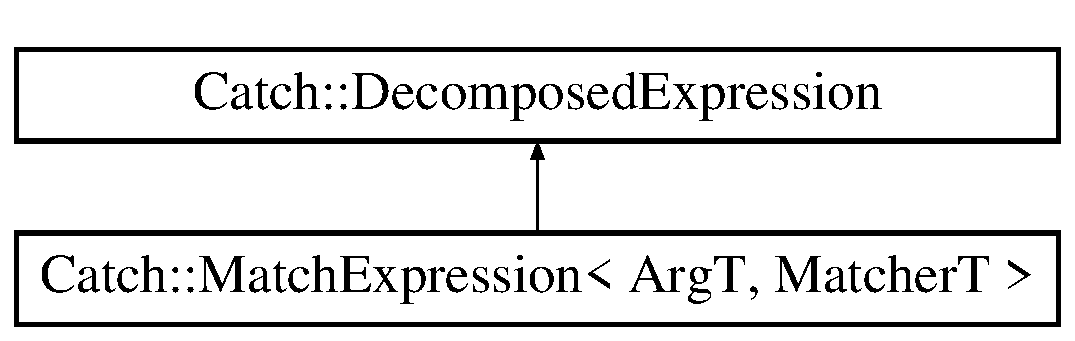
\includegraphics[height=2.000000cm]{classCatch_1_1MatchExpression}
\end{center}
\end{figure}
\subsection*{Public Member Functions}
\begin{DoxyCompactItemize}
\item 
\hyperlink{classCatch_1_1MatchExpression_a506f25bad7970cb35f9dbe54763a8ca5}{Match\-Expression} (Arg\-T arg, Matcher\-T matcher, char const $\ast$matcher\-String)
\item 
virtual bool \hyperlink{classCatch_1_1MatchExpression_ac4edf6e9a6e5762a487db1486d0d1f45}{is\-Binary\-Expression} () const \hyperlink{catch_8hpp_a8ecdce4d3f57835f707915ae831eb847}{C\-A\-T\-C\-H\-\_\-\-O\-V\-E\-R\-R\-I\-D\-E}
\item 
virtual void \hyperlink{classCatch_1_1MatchExpression_a4410a93bc5b8241eb2502f400fce7ec4}{reconstruct\-Expression} (std\-::string \&dest) const \hyperlink{catch_8hpp_a8ecdce4d3f57835f707915ae831eb847}{C\-A\-T\-C\-H\-\_\-\-O\-V\-E\-R\-R\-I\-D\-E}
\end{DoxyCompactItemize}


\subsection{Constructor \& Destructor Documentation}
\hypertarget{classCatch_1_1MatchExpression_a506f25bad7970cb35f9dbe54763a8ca5}{\index{Catch\-::\-Match\-Expression@{Catch\-::\-Match\-Expression}!Match\-Expression@{Match\-Expression}}
\index{Match\-Expression@{Match\-Expression}!Catch::MatchExpression@{Catch\-::\-Match\-Expression}}
\subsubsection[{Match\-Expression}]{\setlength{\rightskip}{0pt plus 5cm}template$<$typename Arg\-T , typename Matcher\-T $>$ {\bf Catch\-::\-Match\-Expression}$<$ Arg\-T, Matcher\-T $>$\-::{\bf Match\-Expression} (
\begin{DoxyParamCaption}
\item[{Arg\-T}]{arg, }
\item[{Matcher\-T}]{matcher, }
\item[{char const $\ast$}]{matcher\-String}
\end{DoxyParamCaption}
)\hspace{0.3cm}{\ttfamily [inline]}}}\label{classCatch_1_1MatchExpression_a506f25bad7970cb35f9dbe54763a8ca5}


\subsection{Member Function Documentation}
\hypertarget{classCatch_1_1MatchExpression_ac4edf6e9a6e5762a487db1486d0d1f45}{\index{Catch\-::\-Match\-Expression@{Catch\-::\-Match\-Expression}!is\-Binary\-Expression@{is\-Binary\-Expression}}
\index{is\-Binary\-Expression@{is\-Binary\-Expression}!Catch::MatchExpression@{Catch\-::\-Match\-Expression}}
\subsubsection[{is\-Binary\-Expression}]{\setlength{\rightskip}{0pt plus 5cm}template$<$typename Arg\-T , typename Matcher\-T $>$ virtual bool {\bf Catch\-::\-Match\-Expression}$<$ Arg\-T, Matcher\-T $>$\-::is\-Binary\-Expression (
\begin{DoxyParamCaption}
{}
\end{DoxyParamCaption}
) const\hspace{0.3cm}{\ttfamily [inline]}, {\ttfamily [virtual]}}}\label{classCatch_1_1MatchExpression_ac4edf6e9a6e5762a487db1486d0d1f45}


Reimplemented from \hyperlink{structCatch_1_1DecomposedExpression_af08ea5b188f04b0f441d8e4cdc340452}{Catch\-::\-Decomposed\-Expression}.

\hypertarget{classCatch_1_1MatchExpression_a4410a93bc5b8241eb2502f400fce7ec4}{\index{Catch\-::\-Match\-Expression@{Catch\-::\-Match\-Expression}!reconstruct\-Expression@{reconstruct\-Expression}}
\index{reconstruct\-Expression@{reconstruct\-Expression}!Catch::MatchExpression@{Catch\-::\-Match\-Expression}}
\subsubsection[{reconstruct\-Expression}]{\setlength{\rightskip}{0pt plus 5cm}template$<$typename Arg\-T , typename Matcher\-T $>$ virtual void {\bf Catch\-::\-Match\-Expression}$<$ Arg\-T, Matcher\-T $>$\-::reconstruct\-Expression (
\begin{DoxyParamCaption}
\item[{std\-::string \&}]{dest}
\end{DoxyParamCaption}
) const\hspace{0.3cm}{\ttfamily [inline]}, {\ttfamily [virtual]}}}\label{classCatch_1_1MatchExpression_a4410a93bc5b8241eb2502f400fce7ec4}


Implements \hyperlink{structCatch_1_1DecomposedExpression_a9ce7f356dc96f11f80e40c82f5aa7e55}{Catch\-::\-Decomposed\-Expression}.



The documentation for this class was generated from the following file\-:\begin{DoxyCompactItemize}
\item 
/home/alexander/\-Un\-B/\-M\-P/\-Trabalho\-\_\-2\-\_\-\-M\-P\-\_\-\-Alexander\-\_\-13\-\_\-0039853/include/\hyperlink{catch_8hpp}{catch.\-hpp}\end{DoxyCompactItemize}

\hypertarget{structCatch_1_1Matchers_1_1Impl_1_1MatchNotOf}{\section{Catch\-:\-:Matchers\-:\-:Impl\-:\-:Match\-Not\-Of$<$ Arg\-T $>$ Struct Template Reference}
\label{structCatch_1_1Matchers_1_1Impl_1_1MatchNotOf}\index{Catch\-::\-Matchers\-::\-Impl\-::\-Match\-Not\-Of$<$ Arg\-T $>$@{Catch\-::\-Matchers\-::\-Impl\-::\-Match\-Not\-Of$<$ Arg\-T $>$}}
}


{\ttfamily \#include $<$catch.\-hpp$>$}

Inheritance diagram for Catch\-:\-:Matchers\-:\-:Impl\-:\-:Match\-Not\-Of$<$ Arg\-T $>$\-:\begin{figure}[H]
\begin{center}
\leavevmode
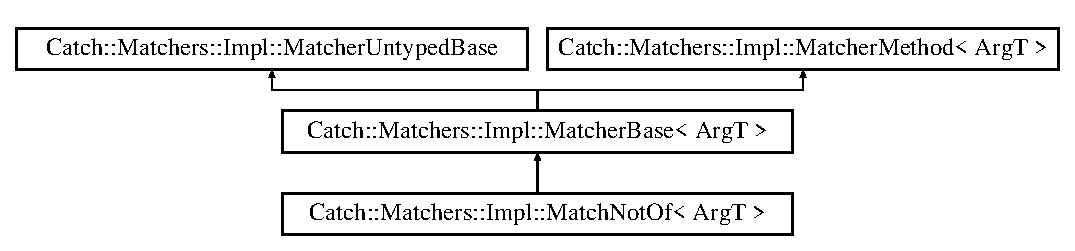
\includegraphics[height=2.926829cm]{structCatch_1_1Matchers_1_1Impl_1_1MatchNotOf}
\end{center}
\end{figure}
\subsection*{Public Member Functions}
\begin{DoxyCompactItemize}
\item 
\hyperlink{structCatch_1_1Matchers_1_1Impl_1_1MatchNotOf_a47afdd9e4c3354cef85adc3186097ae4}{Match\-Not\-Of} (\hyperlink{structCatch_1_1Matchers_1_1Impl_1_1MatcherBase}{Matcher\-Base}$<$ Arg\-T $>$ const \&underlying\-Matcher)
\item 
virtual bool \hyperlink{structCatch_1_1Matchers_1_1Impl_1_1MatchNotOf_a1b9ad6566e4ab0f292d2903f557307cc}{match} (Arg\-T const \&arg) const \hyperlink{catch_8hpp_a8ecdce4d3f57835f707915ae831eb847}{C\-A\-T\-C\-H\-\_\-\-O\-V\-E\-R\-R\-I\-D\-E}
\item 
virtual std\-::string \hyperlink{structCatch_1_1Matchers_1_1Impl_1_1MatchNotOf_a62bdc7dcb9ff000438a4ed3d5483a248}{describe} () const \hyperlink{catch_8hpp_a8ecdce4d3f57835f707915ae831eb847}{C\-A\-T\-C\-H\-\_\-\-O\-V\-E\-R\-R\-I\-D\-E}
\end{DoxyCompactItemize}
\subsection*{Public Attributes}
\begin{DoxyCompactItemize}
\item 
\hyperlink{structCatch_1_1Matchers_1_1Impl_1_1MatcherBase}{Matcher\-Base}$<$ Arg\-T $>$ const \& \hyperlink{structCatch_1_1Matchers_1_1Impl_1_1MatchNotOf_af7ac67f112b0e93796b048a47329aad4}{m\-\_\-underlying\-Matcher}
\end{DoxyCompactItemize}
\subsection*{Additional Inherited Members}


\subsection{Constructor \& Destructor Documentation}
\hypertarget{structCatch_1_1Matchers_1_1Impl_1_1MatchNotOf_a47afdd9e4c3354cef85adc3186097ae4}{\index{Catch\-::\-Matchers\-::\-Impl\-::\-Match\-Not\-Of@{Catch\-::\-Matchers\-::\-Impl\-::\-Match\-Not\-Of}!Match\-Not\-Of@{Match\-Not\-Of}}
\index{Match\-Not\-Of@{Match\-Not\-Of}!Catch::Matchers::Impl::MatchNotOf@{Catch\-::\-Matchers\-::\-Impl\-::\-Match\-Not\-Of}}
\subsubsection[{Match\-Not\-Of}]{\setlength{\rightskip}{0pt plus 5cm}template$<$typename Arg\-T$>$ {\bf Catch\-::\-Matchers\-::\-Impl\-::\-Match\-Not\-Of}$<$ Arg\-T $>$\-::{\bf Match\-Not\-Of} (
\begin{DoxyParamCaption}
\item[{{\bf Matcher\-Base}$<$ Arg\-T $>$ const \&}]{underlying\-Matcher}
\end{DoxyParamCaption}
)\hspace{0.3cm}{\ttfamily [inline]}}}\label{structCatch_1_1Matchers_1_1Impl_1_1MatchNotOf_a47afdd9e4c3354cef85adc3186097ae4}


\subsection{Member Function Documentation}
\hypertarget{structCatch_1_1Matchers_1_1Impl_1_1MatchNotOf_a62bdc7dcb9ff000438a4ed3d5483a248}{\index{Catch\-::\-Matchers\-::\-Impl\-::\-Match\-Not\-Of@{Catch\-::\-Matchers\-::\-Impl\-::\-Match\-Not\-Of}!describe@{describe}}
\index{describe@{describe}!Catch::Matchers::Impl::MatchNotOf@{Catch\-::\-Matchers\-::\-Impl\-::\-Match\-Not\-Of}}
\subsubsection[{describe}]{\setlength{\rightskip}{0pt plus 5cm}template$<$typename Arg\-T$>$ virtual std\-::string {\bf Catch\-::\-Matchers\-::\-Impl\-::\-Match\-Not\-Of}$<$ Arg\-T $>$\-::describe (
\begin{DoxyParamCaption}
{}
\end{DoxyParamCaption}
) const\hspace{0.3cm}{\ttfamily [inline]}, {\ttfamily [virtual]}}}\label{structCatch_1_1Matchers_1_1Impl_1_1MatchNotOf_a62bdc7dcb9ff000438a4ed3d5483a248}


Implements \hyperlink{classCatch_1_1Matchers_1_1Impl_1_1MatcherUntypedBase_a91d3a907dbfcbb596077df24f6e11fe2}{Catch\-::\-Matchers\-::\-Impl\-::\-Matcher\-Untyped\-Base}.

\hypertarget{structCatch_1_1Matchers_1_1Impl_1_1MatchNotOf_a1b9ad6566e4ab0f292d2903f557307cc}{\index{Catch\-::\-Matchers\-::\-Impl\-::\-Match\-Not\-Of@{Catch\-::\-Matchers\-::\-Impl\-::\-Match\-Not\-Of}!match@{match}}
\index{match@{match}!Catch::Matchers::Impl::MatchNotOf@{Catch\-::\-Matchers\-::\-Impl\-::\-Match\-Not\-Of}}
\subsubsection[{match}]{\setlength{\rightskip}{0pt plus 5cm}template$<$typename Arg\-T$>$ virtual bool {\bf Catch\-::\-Matchers\-::\-Impl\-::\-Match\-Not\-Of}$<$ Arg\-T $>$\-::match (
\begin{DoxyParamCaption}
\item[{Arg\-T const \&}]{arg}
\end{DoxyParamCaption}
) const\hspace{0.3cm}{\ttfamily [inline]}, {\ttfamily [virtual]}}}\label{structCatch_1_1Matchers_1_1Impl_1_1MatchNotOf_a1b9ad6566e4ab0f292d2903f557307cc}


Implements \hyperlink{structCatch_1_1Matchers_1_1Impl_1_1MatcherMethod_ae0920ff9e817acf08e1bb0cbcb044e30}{Catch\-::\-Matchers\-::\-Impl\-::\-Matcher\-Method$<$ Arg\-T $>$}.



\subsection{Member Data Documentation}
\hypertarget{structCatch_1_1Matchers_1_1Impl_1_1MatchNotOf_af7ac67f112b0e93796b048a47329aad4}{\index{Catch\-::\-Matchers\-::\-Impl\-::\-Match\-Not\-Of@{Catch\-::\-Matchers\-::\-Impl\-::\-Match\-Not\-Of}!m\-\_\-underlying\-Matcher@{m\-\_\-underlying\-Matcher}}
\index{m\-\_\-underlying\-Matcher@{m\-\_\-underlying\-Matcher}!Catch::Matchers::Impl::MatchNotOf@{Catch\-::\-Matchers\-::\-Impl\-::\-Match\-Not\-Of}}
\subsubsection[{m\-\_\-underlying\-Matcher}]{\setlength{\rightskip}{0pt plus 5cm}template$<$typename Arg\-T$>$ {\bf Matcher\-Base}$<$Arg\-T$>$ const\& {\bf Catch\-::\-Matchers\-::\-Impl\-::\-Match\-Not\-Of}$<$ Arg\-T $>$\-::m\-\_\-underlying\-Matcher}}\label{structCatch_1_1Matchers_1_1Impl_1_1MatchNotOf_af7ac67f112b0e93796b048a47329aad4}


The documentation for this struct was generated from the following file\-:\begin{DoxyCompactItemize}
\item 
/home/alexander/\-Un\-B/\-M\-P/\-Trabalho\-\_\-2\-\_\-\-M\-P\-\_\-\-Alexander\-\_\-13\-\_\-0039853/include/\hyperlink{catch_8hpp}{catch.\-hpp}\end{DoxyCompactItemize}

\hypertarget{structCatch_1_1MessageBuilder}{\section{Catch\-:\-:Message\-Builder Struct Reference}
\label{structCatch_1_1MessageBuilder}\index{Catch\-::\-Message\-Builder@{Catch\-::\-Message\-Builder}}
}


{\ttfamily \#include $<$catch.\-hpp$>$}

\subsection*{Public Member Functions}
\begin{DoxyCompactItemize}
\item 
\hyperlink{structCatch_1_1MessageBuilder_ab0c6378e722680bf58852c6ee2b6e724}{Message\-Builder} (std\-::string const \&macro\-Name, \hyperlink{structCatch_1_1SourceLineInfo}{Source\-Line\-Info} const \&line\-Info, \hyperlink{structCatch_1_1ResultWas_a624e1ee3661fcf6094ceef1f654601ef}{Result\-Was\-::\-Of\-Type} type)
\item 
{\footnotesize template$<$typename T $>$ }\\\hyperlink{structCatch_1_1MessageBuilder}{Message\-Builder} \& \hyperlink{structCatch_1_1MessageBuilder_a20fa48d069b20dddcc2d3df8abb123c1}{operator$<$$<$} (T const \&value)
\end{DoxyCompactItemize}
\subsection*{Public Attributes}
\begin{DoxyCompactItemize}
\item 
\hyperlink{structCatch_1_1MessageInfo}{Message\-Info} \hyperlink{structCatch_1_1MessageBuilder_a979f1c2b36d78f80ee275bfa5ba0209f}{m\-\_\-info}
\item 
std\-::ostringstream \hyperlink{structCatch_1_1MessageBuilder_a6488ab0cc4ea52affc9c0612c7c5df6b}{m\-\_\-stream}
\end{DoxyCompactItemize}


\subsection{Constructor \& Destructor Documentation}
\hypertarget{structCatch_1_1MessageBuilder_ab0c6378e722680bf58852c6ee2b6e724}{\index{Catch\-::\-Message\-Builder@{Catch\-::\-Message\-Builder}!Message\-Builder@{Message\-Builder}}
\index{Message\-Builder@{Message\-Builder}!Catch::MessageBuilder@{Catch\-::\-Message\-Builder}}
\subsubsection[{Message\-Builder}]{\setlength{\rightskip}{0pt plus 5cm}Catch\-::\-Message\-Builder\-::\-Message\-Builder (
\begin{DoxyParamCaption}
\item[{std\-::string const \&}]{macro\-Name, }
\item[{{\bf Source\-Line\-Info} const \&}]{line\-Info, }
\item[{{\bf Result\-Was\-::\-Of\-Type}}]{type}
\end{DoxyParamCaption}
)\hspace{0.3cm}{\ttfamily [inline]}}}\label{structCatch_1_1MessageBuilder_ab0c6378e722680bf58852c6ee2b6e724}


\subsection{Member Function Documentation}
\hypertarget{structCatch_1_1MessageBuilder_a20fa48d069b20dddcc2d3df8abb123c1}{\index{Catch\-::\-Message\-Builder@{Catch\-::\-Message\-Builder}!operator$<$$<$@{operator$<$$<$}}
\index{operator$<$$<$@{operator$<$$<$}!Catch::MessageBuilder@{Catch\-::\-Message\-Builder}}
\subsubsection[{operator$<$$<$}]{\setlength{\rightskip}{0pt plus 5cm}template$<$typename T $>$ {\bf Message\-Builder}\& Catch\-::\-Message\-Builder\-::operator$<$$<$ (
\begin{DoxyParamCaption}
\item[{T const \&}]{value}
\end{DoxyParamCaption}
)\hspace{0.3cm}{\ttfamily [inline]}}}\label{structCatch_1_1MessageBuilder_a20fa48d069b20dddcc2d3df8abb123c1}


\subsection{Member Data Documentation}
\hypertarget{structCatch_1_1MessageBuilder_a979f1c2b36d78f80ee275bfa5ba0209f}{\index{Catch\-::\-Message\-Builder@{Catch\-::\-Message\-Builder}!m\-\_\-info@{m\-\_\-info}}
\index{m\-\_\-info@{m\-\_\-info}!Catch::MessageBuilder@{Catch\-::\-Message\-Builder}}
\subsubsection[{m\-\_\-info}]{\setlength{\rightskip}{0pt plus 5cm}{\bf Message\-Info} Catch\-::\-Message\-Builder\-::m\-\_\-info}}\label{structCatch_1_1MessageBuilder_a979f1c2b36d78f80ee275bfa5ba0209f}
\hypertarget{structCatch_1_1MessageBuilder_a6488ab0cc4ea52affc9c0612c7c5df6b}{\index{Catch\-::\-Message\-Builder@{Catch\-::\-Message\-Builder}!m\-\_\-stream@{m\-\_\-stream}}
\index{m\-\_\-stream@{m\-\_\-stream}!Catch::MessageBuilder@{Catch\-::\-Message\-Builder}}
\subsubsection[{m\-\_\-stream}]{\setlength{\rightskip}{0pt plus 5cm}std\-::ostringstream Catch\-::\-Message\-Builder\-::m\-\_\-stream}}\label{structCatch_1_1MessageBuilder_a6488ab0cc4ea52affc9c0612c7c5df6b}


The documentation for this struct was generated from the following file\-:\begin{DoxyCompactItemize}
\item 
/home/alexander/\-Un\-B/\-M\-P/\-Trabalho\-\_\-2\-\_\-\-M\-P\-\_\-\-Alexander\-\_\-13\-\_\-0039853/include/\hyperlink{catch_8hpp}{catch.\-hpp}\end{DoxyCompactItemize}

\hypertarget{structCatch_1_1MessageInfo}{\section{Catch\-:\-:Message\-Info Struct Reference}
\label{structCatch_1_1MessageInfo}\index{Catch\-::\-Message\-Info@{Catch\-::\-Message\-Info}}
}


{\ttfamily \#include $<$catch.\-hpp$>$}

\subsection*{Public Member Functions}
\begin{DoxyCompactItemize}
\item 
\hyperlink{structCatch_1_1MessageInfo_a2e336c33ebef7af3c1bbae6a56e14f8a}{Message\-Info} (std\-::string const \&\-\_\-macro\-Name, \hyperlink{structCatch_1_1SourceLineInfo}{Source\-Line\-Info} const \&\-\_\-line\-Info, \hyperlink{structCatch_1_1ResultWas_a624e1ee3661fcf6094ceef1f654601ef}{Result\-Was\-::\-Of\-Type} \-\_\-type)
\item 
bool \hyperlink{structCatch_1_1MessageInfo_a30fe117138e568c5a9dfdabb7de6e790}{operator==} (\hyperlink{structCatch_1_1MessageInfo}{Message\-Info} const \&other) const 
\item 
bool \hyperlink{structCatch_1_1MessageInfo_a7a2b1ec3772cd35176e2ee25a94be16a}{operator$<$} (\hyperlink{structCatch_1_1MessageInfo}{Message\-Info} const \&other) const 
\end{DoxyCompactItemize}
\subsection*{Public Attributes}
\begin{DoxyCompactItemize}
\item 
std\-::string \hyperlink{structCatch_1_1MessageInfo_a156ade4b3cc731f6ec7b542ae47ba8e3}{macro\-Name}
\item 
\hyperlink{structCatch_1_1SourceLineInfo}{Source\-Line\-Info} \hyperlink{structCatch_1_1MessageInfo_a985165328723e599696ebd8e43195cc5}{line\-Info}
\item 
\hyperlink{structCatch_1_1ResultWas_a624e1ee3661fcf6094ceef1f654601ef}{Result\-Was\-::\-Of\-Type} \hyperlink{structCatch_1_1MessageInfo_ae928b9117465c696e45951d9d0284e78}{type}
\item 
std\-::string \hyperlink{structCatch_1_1MessageInfo_ab6cd06e050bf426c6577502a5c50e256}{message}
\item 
unsigned int \hyperlink{structCatch_1_1MessageInfo_a7f4f57ea21e50160adefce7b68a781d6}{sequence}
\end{DoxyCompactItemize}


\subsection{Constructor \& Destructor Documentation}
\hypertarget{structCatch_1_1MessageInfo_a2e336c33ebef7af3c1bbae6a56e14f8a}{\index{Catch\-::\-Message\-Info@{Catch\-::\-Message\-Info}!Message\-Info@{Message\-Info}}
\index{Message\-Info@{Message\-Info}!Catch::MessageInfo@{Catch\-::\-Message\-Info}}
\subsubsection[{Message\-Info}]{\setlength{\rightskip}{0pt plus 5cm}Catch\-::\-Message\-Info\-::\-Message\-Info (
\begin{DoxyParamCaption}
\item[{std\-::string const \&}]{\-\_\-macro\-Name, }
\item[{{\bf Source\-Line\-Info} const \&}]{\-\_\-line\-Info, }
\item[{{\bf Result\-Was\-::\-Of\-Type}}]{\-\_\-type}
\end{DoxyParamCaption}
)}}\label{structCatch_1_1MessageInfo_a2e336c33ebef7af3c1bbae6a56e14f8a}


\subsection{Member Function Documentation}
\hypertarget{structCatch_1_1MessageInfo_a7a2b1ec3772cd35176e2ee25a94be16a}{\index{Catch\-::\-Message\-Info@{Catch\-::\-Message\-Info}!operator$<$@{operator$<$}}
\index{operator$<$@{operator$<$}!Catch::MessageInfo@{Catch\-::\-Message\-Info}}
\subsubsection[{operator$<$}]{\setlength{\rightskip}{0pt plus 5cm}bool Catch\-::\-Message\-Info\-::operator$<$ (
\begin{DoxyParamCaption}
\item[{{\bf Message\-Info} const \&}]{other}
\end{DoxyParamCaption}
) const\hspace{0.3cm}{\ttfamily [inline]}}}\label{structCatch_1_1MessageInfo_a7a2b1ec3772cd35176e2ee25a94be16a}
\hypertarget{structCatch_1_1MessageInfo_a30fe117138e568c5a9dfdabb7de6e790}{\index{Catch\-::\-Message\-Info@{Catch\-::\-Message\-Info}!operator==@{operator==}}
\index{operator==@{operator==}!Catch::MessageInfo@{Catch\-::\-Message\-Info}}
\subsubsection[{operator==}]{\setlength{\rightskip}{0pt plus 5cm}bool Catch\-::\-Message\-Info\-::operator== (
\begin{DoxyParamCaption}
\item[{{\bf Message\-Info} const \&}]{other}
\end{DoxyParamCaption}
) const\hspace{0.3cm}{\ttfamily [inline]}}}\label{structCatch_1_1MessageInfo_a30fe117138e568c5a9dfdabb7de6e790}


\subsection{Member Data Documentation}
\hypertarget{structCatch_1_1MessageInfo_a985165328723e599696ebd8e43195cc5}{\index{Catch\-::\-Message\-Info@{Catch\-::\-Message\-Info}!line\-Info@{line\-Info}}
\index{line\-Info@{line\-Info}!Catch::MessageInfo@{Catch\-::\-Message\-Info}}
\subsubsection[{line\-Info}]{\setlength{\rightskip}{0pt plus 5cm}{\bf Source\-Line\-Info} Catch\-::\-Message\-Info\-::line\-Info}}\label{structCatch_1_1MessageInfo_a985165328723e599696ebd8e43195cc5}
\hypertarget{structCatch_1_1MessageInfo_a156ade4b3cc731f6ec7b542ae47ba8e3}{\index{Catch\-::\-Message\-Info@{Catch\-::\-Message\-Info}!macro\-Name@{macro\-Name}}
\index{macro\-Name@{macro\-Name}!Catch::MessageInfo@{Catch\-::\-Message\-Info}}
\subsubsection[{macro\-Name}]{\setlength{\rightskip}{0pt plus 5cm}std\-::string Catch\-::\-Message\-Info\-::macro\-Name}}\label{structCatch_1_1MessageInfo_a156ade4b3cc731f6ec7b542ae47ba8e3}
\hypertarget{structCatch_1_1MessageInfo_ab6cd06e050bf426c6577502a5c50e256}{\index{Catch\-::\-Message\-Info@{Catch\-::\-Message\-Info}!message@{message}}
\index{message@{message}!Catch::MessageInfo@{Catch\-::\-Message\-Info}}
\subsubsection[{message}]{\setlength{\rightskip}{0pt plus 5cm}std\-::string Catch\-::\-Message\-Info\-::message}}\label{structCatch_1_1MessageInfo_ab6cd06e050bf426c6577502a5c50e256}
\hypertarget{structCatch_1_1MessageInfo_a7f4f57ea21e50160adefce7b68a781d6}{\index{Catch\-::\-Message\-Info@{Catch\-::\-Message\-Info}!sequence@{sequence}}
\index{sequence@{sequence}!Catch::MessageInfo@{Catch\-::\-Message\-Info}}
\subsubsection[{sequence}]{\setlength{\rightskip}{0pt plus 5cm}unsigned int Catch\-::\-Message\-Info\-::sequence}}\label{structCatch_1_1MessageInfo_a7f4f57ea21e50160adefce7b68a781d6}
\hypertarget{structCatch_1_1MessageInfo_ae928b9117465c696e45951d9d0284e78}{\index{Catch\-::\-Message\-Info@{Catch\-::\-Message\-Info}!type@{type}}
\index{type@{type}!Catch::MessageInfo@{Catch\-::\-Message\-Info}}
\subsubsection[{type}]{\setlength{\rightskip}{0pt plus 5cm}{\bf Result\-Was\-::\-Of\-Type} Catch\-::\-Message\-Info\-::type}}\label{structCatch_1_1MessageInfo_ae928b9117465c696e45951d9d0284e78}


The documentation for this struct was generated from the following file\-:\begin{DoxyCompactItemize}
\item 
/home/alexander/\-Un\-B/\-M\-P/\-Trabalho\-\_\-2\-\_\-\-M\-P\-\_\-\-Alexander\-\_\-13\-\_\-0039853/include/\hyperlink{catch_8hpp}{catch.\-hpp}\end{DoxyCompactItemize}

\hypertarget{classCatch_1_1MethodTestCase}{\section{Catch\-:\-:Method\-Test\-Case$<$ C $>$ Class Template Reference}
\label{classCatch_1_1MethodTestCase}\index{Catch\-::\-Method\-Test\-Case$<$ C $>$@{Catch\-::\-Method\-Test\-Case$<$ C $>$}}
}


{\ttfamily \#include $<$catch.\-hpp$>$}

Inheritance diagram for Catch\-:\-:Method\-Test\-Case$<$ C $>$\-:\begin{figure}[H]
\begin{center}
\leavevmode
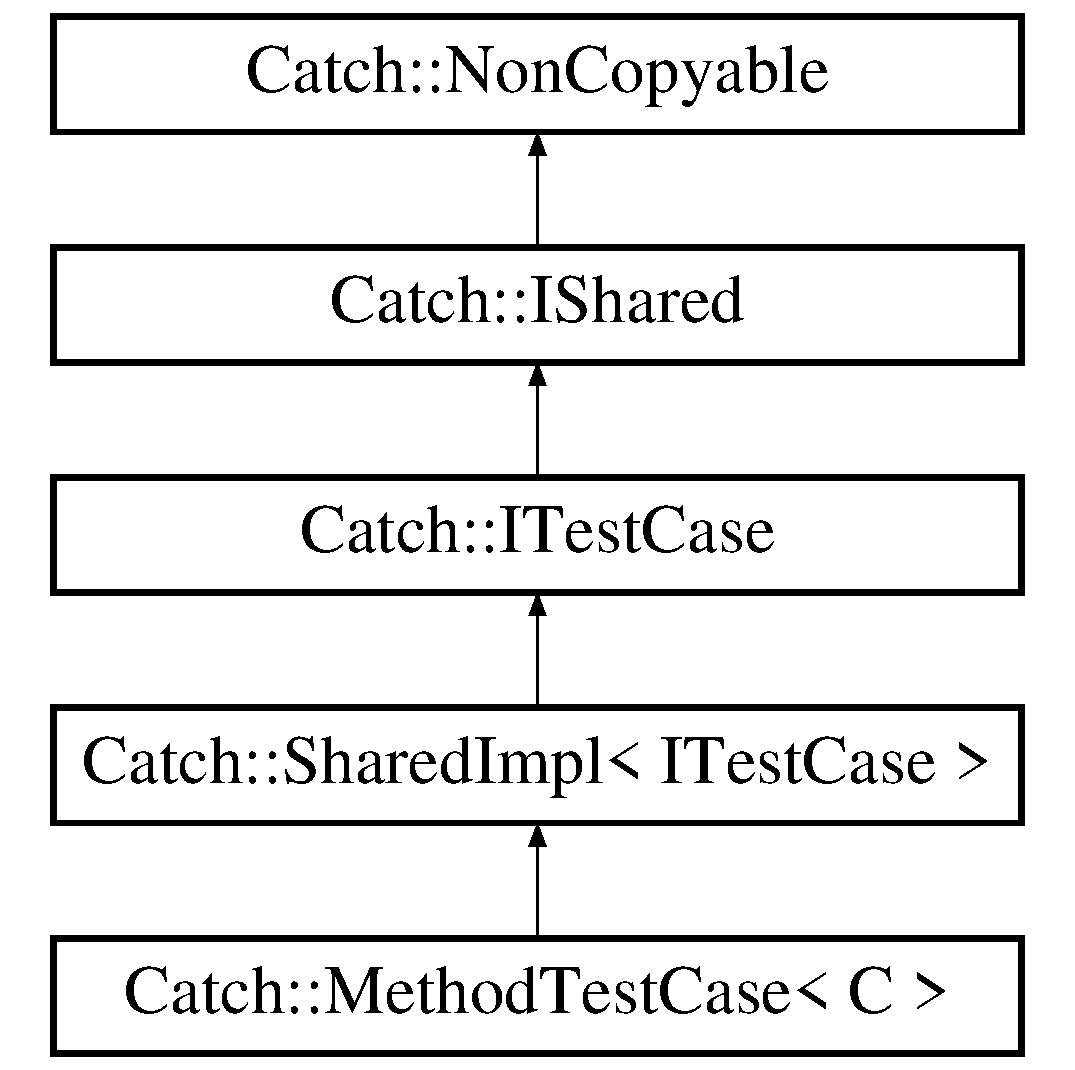
\includegraphics[height=5.000000cm]{classCatch_1_1MethodTestCase}
\end{center}
\end{figure}
\subsection*{Public Member Functions}
\begin{DoxyCompactItemize}
\item 
\hyperlink{classCatch_1_1MethodTestCase_a7b043b85dae371358255dd9dc6582e7b}{Method\-Test\-Case} (void(C\-::$\ast$method)())
\item 
virtual void \hyperlink{classCatch_1_1MethodTestCase_a39cc4b760dd71adc3f7550bc1e7eb697}{invoke} () const 
\end{DoxyCompactItemize}
\subsection*{Additional Inherited Members}


\subsection{Constructor \& Destructor Documentation}
\hypertarget{classCatch_1_1MethodTestCase_a7b043b85dae371358255dd9dc6582e7b}{\index{Catch\-::\-Method\-Test\-Case@{Catch\-::\-Method\-Test\-Case}!Method\-Test\-Case@{Method\-Test\-Case}}
\index{Method\-Test\-Case@{Method\-Test\-Case}!Catch::MethodTestCase@{Catch\-::\-Method\-Test\-Case}}
\subsubsection[{Method\-Test\-Case}]{\setlength{\rightskip}{0pt plus 5cm}template$<$typename C $>$ {\bf Catch\-::\-Method\-Test\-Case}$<$ C $>$\-::{\bf Method\-Test\-Case} (
\begin{DoxyParamCaption}
\item[{void(C\-::$\ast$)()}]{method}
\end{DoxyParamCaption}
)\hspace{0.3cm}{\ttfamily [inline]}}}\label{classCatch_1_1MethodTestCase_a7b043b85dae371358255dd9dc6582e7b}


\subsection{Member Function Documentation}
\hypertarget{classCatch_1_1MethodTestCase_a39cc4b760dd71adc3f7550bc1e7eb697}{\index{Catch\-::\-Method\-Test\-Case@{Catch\-::\-Method\-Test\-Case}!invoke@{invoke}}
\index{invoke@{invoke}!Catch::MethodTestCase@{Catch\-::\-Method\-Test\-Case}}
\subsubsection[{invoke}]{\setlength{\rightskip}{0pt plus 5cm}template$<$typename C $>$ virtual void {\bf Catch\-::\-Method\-Test\-Case}$<$ C $>$\-::invoke (
\begin{DoxyParamCaption}
{}
\end{DoxyParamCaption}
) const\hspace{0.3cm}{\ttfamily [inline]}, {\ttfamily [virtual]}}}\label{classCatch_1_1MethodTestCase_a39cc4b760dd71adc3f7550bc1e7eb697}


Implements \hyperlink{structCatch_1_1ITestCase_a678825e62e7c17297621cfeb65588c34}{Catch\-::\-I\-Test\-Case}.



The documentation for this class was generated from the following file\-:\begin{DoxyCompactItemize}
\item 
/home/alexander/\-Un\-B/\-M\-P/\-Trabalho\-\_\-2\-\_\-\-M\-P\-\_\-\-Alexander\-\_\-13\-\_\-0039853/include/\hyperlink{catch_8hpp}{catch.\-hpp}\end{DoxyCompactItemize}

\hypertarget{structCatch_1_1NameAndDesc}{\section{Catch\-:\-:Name\-And\-Desc Struct Reference}
\label{structCatch_1_1NameAndDesc}\index{Catch\-::\-Name\-And\-Desc@{Catch\-::\-Name\-And\-Desc}}
}


{\ttfamily \#include $<$catch.\-hpp$>$}

\subsection*{Public Member Functions}
\begin{DoxyCompactItemize}
\item 
\hyperlink{structCatch_1_1NameAndDesc_a189ceb9942fb5f6635140d6a09fc843a}{Name\-And\-Desc} (const char $\ast$\-\_\-name=\char`\"{}\char`\"{}, const char $\ast$\-\_\-description=\char`\"{}\char`\"{})
\end{DoxyCompactItemize}
\subsection*{Public Attributes}
\begin{DoxyCompactItemize}
\item 
const char $\ast$ \hyperlink{structCatch_1_1NameAndDesc_a374b4ed8be3cf98be20ebde5273bde51}{name}
\item 
const char $\ast$ \hyperlink{structCatch_1_1NameAndDesc_a3463a23ff65ce494fc380452b57b7970}{description}
\end{DoxyCompactItemize}


\subsection{Constructor \& Destructor Documentation}
\hypertarget{structCatch_1_1NameAndDesc_a189ceb9942fb5f6635140d6a09fc843a}{\index{Catch\-::\-Name\-And\-Desc@{Catch\-::\-Name\-And\-Desc}!Name\-And\-Desc@{Name\-And\-Desc}}
\index{Name\-And\-Desc@{Name\-And\-Desc}!Catch::NameAndDesc@{Catch\-::\-Name\-And\-Desc}}
\subsubsection[{Name\-And\-Desc}]{\setlength{\rightskip}{0pt plus 5cm}Catch\-::\-Name\-And\-Desc\-::\-Name\-And\-Desc (
\begin{DoxyParamCaption}
\item[{const char $\ast$}]{\-\_\-name = {\ttfamily \char`\"{}\char`\"{}}, }
\item[{const char $\ast$}]{\-\_\-description = {\ttfamily \char`\"{}\char`\"{}}}
\end{DoxyParamCaption}
)\hspace{0.3cm}{\ttfamily [inline]}}}\label{structCatch_1_1NameAndDesc_a189ceb9942fb5f6635140d6a09fc843a}


\subsection{Member Data Documentation}
\hypertarget{structCatch_1_1NameAndDesc_a3463a23ff65ce494fc380452b57b7970}{\index{Catch\-::\-Name\-And\-Desc@{Catch\-::\-Name\-And\-Desc}!description@{description}}
\index{description@{description}!Catch::NameAndDesc@{Catch\-::\-Name\-And\-Desc}}
\subsubsection[{description}]{\setlength{\rightskip}{0pt plus 5cm}const char$\ast$ Catch\-::\-Name\-And\-Desc\-::description}}\label{structCatch_1_1NameAndDesc_a3463a23ff65ce494fc380452b57b7970}
\hypertarget{structCatch_1_1NameAndDesc_a374b4ed8be3cf98be20ebde5273bde51}{\index{Catch\-::\-Name\-And\-Desc@{Catch\-::\-Name\-And\-Desc}!name@{name}}
\index{name@{name}!Catch::NameAndDesc@{Catch\-::\-Name\-And\-Desc}}
\subsubsection[{name}]{\setlength{\rightskip}{0pt plus 5cm}const char$\ast$ Catch\-::\-Name\-And\-Desc\-::name}}\label{structCatch_1_1NameAndDesc_a374b4ed8be3cf98be20ebde5273bde51}


The documentation for this struct was generated from the following file\-:\begin{DoxyCompactItemize}
\item 
/home/alexander/\-Un\-B/\-M\-P/\-Trabalho\-\_\-2\-\_\-\-M\-P\-\_\-\-Alexander\-\_\-13\-\_\-0039853/include/\hyperlink{catch_8hpp}{catch.\-hpp}\end{DoxyCompactItemize}

\hypertarget{classCatch_1_1NonCopyable}{\section{Catch\-:\-:Non\-Copyable Class Reference}
\label{classCatch_1_1NonCopyable}\index{Catch\-::\-Non\-Copyable@{Catch\-::\-Non\-Copyable}}
}


{\ttfamily \#include $<$catch.\-hpp$>$}

Inheritance diagram for Catch\-:\-:Non\-Copyable\-:\begin{figure}[H]
\begin{center}
\leavevmode
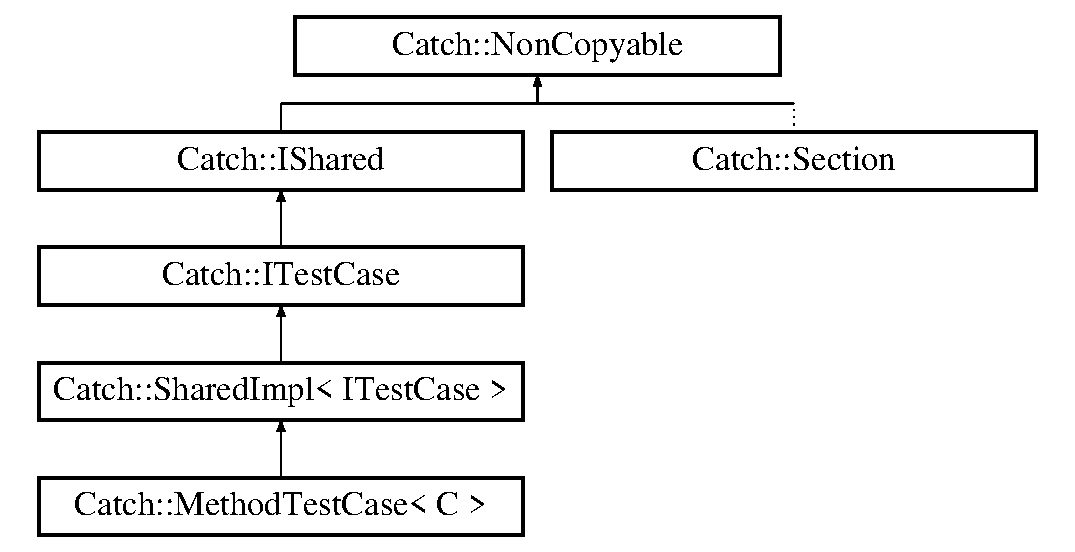
\includegraphics[height=5.000000cm]{classCatch_1_1NonCopyable}
\end{center}
\end{figure}
\subsection*{Protected Member Functions}
\begin{DoxyCompactItemize}
\item 
\hyperlink{classCatch_1_1NonCopyable_a4b492dd5753f9952350fb64dc6cb9fe2}{Non\-Copyable} ()
\item 
virtual \hyperlink{classCatch_1_1NonCopyable_a81254677280fef337eb4a676e91e3293}{$\sim$\-Non\-Copyable} ()
\end{DoxyCompactItemize}


\subsection{Constructor \& Destructor Documentation}
\hypertarget{classCatch_1_1NonCopyable_a4b492dd5753f9952350fb64dc6cb9fe2}{\index{Catch\-::\-Non\-Copyable@{Catch\-::\-Non\-Copyable}!Non\-Copyable@{Non\-Copyable}}
\index{Non\-Copyable@{Non\-Copyable}!Catch::NonCopyable@{Catch\-::\-Non\-Copyable}}
\subsubsection[{Non\-Copyable}]{\setlength{\rightskip}{0pt plus 5cm}Catch\-::\-Non\-Copyable\-::\-Non\-Copyable (
\begin{DoxyParamCaption}
{}
\end{DoxyParamCaption}
)\hspace{0.3cm}{\ttfamily [inline]}, {\ttfamily [protected]}}}\label{classCatch_1_1NonCopyable_a4b492dd5753f9952350fb64dc6cb9fe2}
\hypertarget{classCatch_1_1NonCopyable_a81254677280fef337eb4a676e91e3293}{\index{Catch\-::\-Non\-Copyable@{Catch\-::\-Non\-Copyable}!$\sim$\-Non\-Copyable@{$\sim$\-Non\-Copyable}}
\index{$\sim$\-Non\-Copyable@{$\sim$\-Non\-Copyable}!Catch::NonCopyable@{Catch\-::\-Non\-Copyable}}
\subsubsection[{$\sim$\-Non\-Copyable}]{\setlength{\rightskip}{0pt plus 5cm}virtual Catch\-::\-Non\-Copyable\-::$\sim$\-Non\-Copyable (
\begin{DoxyParamCaption}
{}
\end{DoxyParamCaption}
)\hspace{0.3cm}{\ttfamily [protected]}, {\ttfamily [virtual]}}}\label{classCatch_1_1NonCopyable_a81254677280fef337eb4a676e91e3293}


The documentation for this class was generated from the following file\-:\begin{DoxyCompactItemize}
\item 
/home/alexander/\-Un\-B/\-M\-P/\-Trabalho\-\_\-2\-\_\-\-M\-P\-\_\-\-Alexander\-\_\-13\-\_\-0039853/include/\hyperlink{catch_8hpp}{catch.\-hpp}\end{DoxyCompactItemize}

\hypertarget{classCatch_1_1NotImplementedException}{\section{Catch\-:\-:Not\-Implemented\-Exception Class Reference}
\label{classCatch_1_1NotImplementedException}\index{Catch\-::\-Not\-Implemented\-Exception@{Catch\-::\-Not\-Implemented\-Exception}}
}


{\ttfamily \#include $<$catch.\-hpp$>$}

Inheritance diagram for Catch\-:\-:Not\-Implemented\-Exception\-:\begin{figure}[H]
\begin{center}
\leavevmode
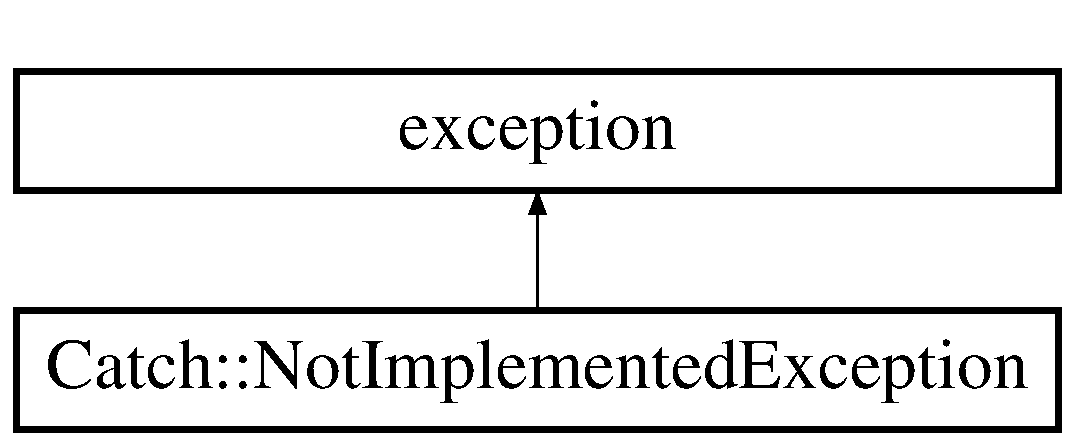
\includegraphics[height=2.000000cm]{classCatch_1_1NotImplementedException}
\end{center}
\end{figure}
\subsection*{Public Member Functions}
\begin{DoxyCompactItemize}
\item 
\hyperlink{classCatch_1_1NotImplementedException_ab4f0a5c39d8ffb72c664e2c07e180634}{Not\-Implemented\-Exception} (\hyperlink{structCatch_1_1SourceLineInfo}{Source\-Line\-Info} const \&line\-Info)
\item 
\hyperlink{classCatch_1_1NotImplementedException_a508a7a833455da2d3c10ea1a9d45e982}{Not\-Implemented\-Exception} (\hyperlink{classCatch_1_1NotImplementedException}{Not\-Implemented\-Exception} const \&)
\item 
virtual \hyperlink{classCatch_1_1NotImplementedException_a557e7312aaa32c37bded019f2b059bcb}{$\sim$\-Not\-Implemented\-Exception} () \hyperlink{catch_8hpp_a0408e94ca73880d41f38852b68eadb3c}{C\-A\-T\-C\-H\-\_\-\-N\-O\-E\-X\-C\-E\-P\-T}
\item 
virtual const char $\ast$ \hyperlink{classCatch_1_1NotImplementedException_ad4c13963f1a8feacda0cd331adda89e3}{what} () const \hyperlink{catch_8hpp_a0408e94ca73880d41f38852b68eadb3c}{C\-A\-T\-C\-H\-\_\-\-N\-O\-E\-X\-C\-E\-P\-T}
\end{DoxyCompactItemize}


\subsection{Constructor \& Destructor Documentation}
\hypertarget{classCatch_1_1NotImplementedException_ab4f0a5c39d8ffb72c664e2c07e180634}{\index{Catch\-::\-Not\-Implemented\-Exception@{Catch\-::\-Not\-Implemented\-Exception}!Not\-Implemented\-Exception@{Not\-Implemented\-Exception}}
\index{Not\-Implemented\-Exception@{Not\-Implemented\-Exception}!Catch::NotImplementedException@{Catch\-::\-Not\-Implemented\-Exception}}
\subsubsection[{Not\-Implemented\-Exception}]{\setlength{\rightskip}{0pt plus 5cm}Catch\-::\-Not\-Implemented\-Exception\-::\-Not\-Implemented\-Exception (
\begin{DoxyParamCaption}
\item[{{\bf Source\-Line\-Info} const \&}]{line\-Info}
\end{DoxyParamCaption}
)}}\label{classCatch_1_1NotImplementedException_ab4f0a5c39d8ffb72c664e2c07e180634}
\hypertarget{classCatch_1_1NotImplementedException_a508a7a833455da2d3c10ea1a9d45e982}{\index{Catch\-::\-Not\-Implemented\-Exception@{Catch\-::\-Not\-Implemented\-Exception}!Not\-Implemented\-Exception@{Not\-Implemented\-Exception}}
\index{Not\-Implemented\-Exception@{Not\-Implemented\-Exception}!Catch::NotImplementedException@{Catch\-::\-Not\-Implemented\-Exception}}
\subsubsection[{Not\-Implemented\-Exception}]{\setlength{\rightskip}{0pt plus 5cm}Catch\-::\-Not\-Implemented\-Exception\-::\-Not\-Implemented\-Exception (
\begin{DoxyParamCaption}
\item[{{\bf Not\-Implemented\-Exception} const \&}]{}
\end{DoxyParamCaption}
)\hspace{0.3cm}{\ttfamily [inline]}}}\label{classCatch_1_1NotImplementedException_a508a7a833455da2d3c10ea1a9d45e982}
\hypertarget{classCatch_1_1NotImplementedException_a557e7312aaa32c37bded019f2b059bcb}{\index{Catch\-::\-Not\-Implemented\-Exception@{Catch\-::\-Not\-Implemented\-Exception}!$\sim$\-Not\-Implemented\-Exception@{$\sim$\-Not\-Implemented\-Exception}}
\index{$\sim$\-Not\-Implemented\-Exception@{$\sim$\-Not\-Implemented\-Exception}!Catch::NotImplementedException@{Catch\-::\-Not\-Implemented\-Exception}}
\subsubsection[{$\sim$\-Not\-Implemented\-Exception}]{\setlength{\rightskip}{0pt plus 5cm}virtual Catch\-::\-Not\-Implemented\-Exception\-::$\sim$\-Not\-Implemented\-Exception (
\begin{DoxyParamCaption}
{}
\end{DoxyParamCaption}
)\hspace{0.3cm}{\ttfamily [inline]}, {\ttfamily [virtual]}}}\label{classCatch_1_1NotImplementedException_a557e7312aaa32c37bded019f2b059bcb}


\subsection{Member Function Documentation}
\hypertarget{classCatch_1_1NotImplementedException_ad4c13963f1a8feacda0cd331adda89e3}{\index{Catch\-::\-Not\-Implemented\-Exception@{Catch\-::\-Not\-Implemented\-Exception}!what@{what}}
\index{what@{what}!Catch::NotImplementedException@{Catch\-::\-Not\-Implemented\-Exception}}
\subsubsection[{what}]{\setlength{\rightskip}{0pt plus 5cm}virtual const char$\ast$ Catch\-::\-Not\-Implemented\-Exception\-::what (
\begin{DoxyParamCaption}
{}
\end{DoxyParamCaption}
) const\hspace{0.3cm}{\ttfamily [virtual]}}}\label{classCatch_1_1NotImplementedException_ad4c13963f1a8feacda0cd331adda89e3}


The documentation for this class was generated from the following file\-:\begin{DoxyCompactItemize}
\item 
/home/alexander/\-Un\-B/\-M\-P/\-Trabalho\-\_\-2\-\_\-\-M\-P\-\_\-\-Alexander\-\_\-13\-\_\-0039853/include/\hyperlink{catch_8hpp}{catch.\-hpp}\end{DoxyCompactItemize}

\hypertarget{structCatch_1_1Internal_1_1OperatorTraits}{\section{Catch\-:\-:Internal\-:\-:Operator\-Traits$<$ Op $>$ Struct Template Reference}
\label{structCatch_1_1Internal_1_1OperatorTraits}\index{Catch\-::\-Internal\-::\-Operator\-Traits$<$ Op $>$@{Catch\-::\-Internal\-::\-Operator\-Traits$<$ Op $>$}}
}


{\ttfamily \#include $<$catch.\-hpp$>$}

\subsection*{Static Public Member Functions}
\begin{DoxyCompactItemize}
\item 
static const char $\ast$ \hyperlink{structCatch_1_1Internal_1_1OperatorTraits_ac6d08082ea33348d42bc4ccbd6d07671}{get\-Name} ()
\end{DoxyCompactItemize}


\subsection{Member Function Documentation}
\hypertarget{structCatch_1_1Internal_1_1OperatorTraits_ac6d08082ea33348d42bc4ccbd6d07671}{\index{Catch\-::\-Internal\-::\-Operator\-Traits@{Catch\-::\-Internal\-::\-Operator\-Traits}!get\-Name@{get\-Name}}
\index{get\-Name@{get\-Name}!Catch::Internal::OperatorTraits@{Catch\-::\-Internal\-::\-Operator\-Traits}}
\subsubsection[{get\-Name}]{\setlength{\rightskip}{0pt plus 5cm}template$<$Operator Op$>$ static const char$\ast$ {\bf Catch\-::\-Internal\-::\-Operator\-Traits}$<$ Op $>$\-::get\-Name (
\begin{DoxyParamCaption}
{}
\end{DoxyParamCaption}
)\hspace{0.3cm}{\ttfamily [inline]}, {\ttfamily [static]}}}\label{structCatch_1_1Internal_1_1OperatorTraits_ac6d08082ea33348d42bc4ccbd6d07671}


The documentation for this struct was generated from the following file\-:\begin{DoxyCompactItemize}
\item 
/home/alexander/\-Un\-B/\-M\-P/\-Trabalho\-\_\-2\-\_\-\-M\-P\-\_\-\-Alexander\-\_\-13\-\_\-0039853/include/\hyperlink{catch_8hpp}{catch.\-hpp}\end{DoxyCompactItemize}

\hypertarget{structCatch_1_1Internal_1_1OperatorTraits_3_01IsEqualTo_01_4}{\section{Catch\-:\-:Internal\-:\-:Operator\-Traits$<$ Is\-Equal\-To $>$ Struct Template Reference}
\label{structCatch_1_1Internal_1_1OperatorTraits_3_01IsEqualTo_01_4}\index{Catch\-::\-Internal\-::\-Operator\-Traits$<$ Is\-Equal\-To $>$@{Catch\-::\-Internal\-::\-Operator\-Traits$<$ Is\-Equal\-To $>$}}
}


{\ttfamily \#include $<$catch.\-hpp$>$}

\subsection*{Static Public Member Functions}
\begin{DoxyCompactItemize}
\item 
static const char $\ast$ \hyperlink{structCatch_1_1Internal_1_1OperatorTraits_3_01IsEqualTo_01_4_addf03ac66f0ed83abcc037a7a327d4f1}{get\-Name} ()
\end{DoxyCompactItemize}


\subsection{Member Function Documentation}
\hypertarget{structCatch_1_1Internal_1_1OperatorTraits_3_01IsEqualTo_01_4_addf03ac66f0ed83abcc037a7a327d4f1}{\index{Catch\-::\-Internal\-::\-Operator\-Traits$<$ Is\-Equal\-To $>$@{Catch\-::\-Internal\-::\-Operator\-Traits$<$ Is\-Equal\-To $>$}!get\-Name@{get\-Name}}
\index{get\-Name@{get\-Name}!Catch::Internal::OperatorTraits< IsEqualTo >@{Catch\-::\-Internal\-::\-Operator\-Traits$<$ Is\-Equal\-To $>$}}
\subsubsection[{get\-Name}]{\setlength{\rightskip}{0pt plus 5cm}static const char$\ast$ {\bf Catch\-::\-Internal\-::\-Operator\-Traits}$<$ {\bf Is\-Equal\-To} $>$\-::get\-Name (
\begin{DoxyParamCaption}
{}
\end{DoxyParamCaption}
)\hspace{0.3cm}{\ttfamily [inline]}, {\ttfamily [static]}}}\label{structCatch_1_1Internal_1_1OperatorTraits_3_01IsEqualTo_01_4_addf03ac66f0ed83abcc037a7a327d4f1}


The documentation for this struct was generated from the following file\-:\begin{DoxyCompactItemize}
\item 
/home/alexander/\-Un\-B/\-M\-P/\-Trabalho\-\_\-2\-\_\-\-M\-P\-\_\-\-Alexander\-\_\-13\-\_\-0039853/include/\hyperlink{catch_8hpp}{catch.\-hpp}\end{DoxyCompactItemize}

\hypertarget{structCatch_1_1Internal_1_1OperatorTraits_3_01IsGreaterThan_01_4}{\section{Catch\-:\-:Internal\-:\-:Operator\-Traits$<$ Is\-Greater\-Than $>$ Struct Template Reference}
\label{structCatch_1_1Internal_1_1OperatorTraits_3_01IsGreaterThan_01_4}\index{Catch\-::\-Internal\-::\-Operator\-Traits$<$ Is\-Greater\-Than $>$@{Catch\-::\-Internal\-::\-Operator\-Traits$<$ Is\-Greater\-Than $>$}}
}


{\ttfamily \#include $<$catch.\-hpp$>$}

\subsection*{Static Public Member Functions}
\begin{DoxyCompactItemize}
\item 
static const char $\ast$ \hyperlink{structCatch_1_1Internal_1_1OperatorTraits_3_01IsGreaterThan_01_4_ab917bfb9ccbe461dc684ee5a34d67d27}{get\-Name} ()
\end{DoxyCompactItemize}


\subsection{Member Function Documentation}
\hypertarget{structCatch_1_1Internal_1_1OperatorTraits_3_01IsGreaterThan_01_4_ab917bfb9ccbe461dc684ee5a34d67d27}{\index{Catch\-::\-Internal\-::\-Operator\-Traits$<$ Is\-Greater\-Than $>$@{Catch\-::\-Internal\-::\-Operator\-Traits$<$ Is\-Greater\-Than $>$}!get\-Name@{get\-Name}}
\index{get\-Name@{get\-Name}!Catch::Internal::OperatorTraits< IsGreaterThan >@{Catch\-::\-Internal\-::\-Operator\-Traits$<$ Is\-Greater\-Than $>$}}
\subsubsection[{get\-Name}]{\setlength{\rightskip}{0pt plus 5cm}static const char$\ast$ {\bf Catch\-::\-Internal\-::\-Operator\-Traits}$<$ {\bf Is\-Greater\-Than} $>$\-::get\-Name (
\begin{DoxyParamCaption}
{}
\end{DoxyParamCaption}
)\hspace{0.3cm}{\ttfamily [inline]}, {\ttfamily [static]}}}\label{structCatch_1_1Internal_1_1OperatorTraits_3_01IsGreaterThan_01_4_ab917bfb9ccbe461dc684ee5a34d67d27}


The documentation for this struct was generated from the following file\-:\begin{DoxyCompactItemize}
\item 
/home/alexander/\-Un\-B/\-M\-P/\-Trabalho\-\_\-2\-\_\-\-M\-P\-\_\-\-Alexander\-\_\-13\-\_\-0039853/include/\hyperlink{catch_8hpp}{catch.\-hpp}\end{DoxyCompactItemize}

\hypertarget{structCatch_1_1Internal_1_1OperatorTraits_3_01IsGreaterThanOrEqualTo_01_4}{\section{Catch\-:\-:Internal\-:\-:Operator\-Traits$<$ Is\-Greater\-Than\-Or\-Equal\-To $>$ Struct Template Reference}
\label{structCatch_1_1Internal_1_1OperatorTraits_3_01IsGreaterThanOrEqualTo_01_4}\index{Catch\-::\-Internal\-::\-Operator\-Traits$<$ Is\-Greater\-Than\-Or\-Equal\-To $>$@{Catch\-::\-Internal\-::\-Operator\-Traits$<$ Is\-Greater\-Than\-Or\-Equal\-To $>$}}
}


{\ttfamily \#include $<$catch.\-hpp$>$}

\subsection*{Static Public Member Functions}
\begin{DoxyCompactItemize}
\item 
static const char $\ast$ \hyperlink{structCatch_1_1Internal_1_1OperatorTraits_3_01IsGreaterThanOrEqualTo_01_4_a76b6f6b0dbaf7d19ebb1b4b4891e719e}{get\-Name} ()
\end{DoxyCompactItemize}


\subsection{Member Function Documentation}
\hypertarget{structCatch_1_1Internal_1_1OperatorTraits_3_01IsGreaterThanOrEqualTo_01_4_a76b6f6b0dbaf7d19ebb1b4b4891e719e}{\index{Catch\-::\-Internal\-::\-Operator\-Traits$<$ Is\-Greater\-Than\-Or\-Equal\-To $>$@{Catch\-::\-Internal\-::\-Operator\-Traits$<$ Is\-Greater\-Than\-Or\-Equal\-To $>$}!get\-Name@{get\-Name}}
\index{get\-Name@{get\-Name}!Catch::Internal::OperatorTraits< IsGreaterThanOrEqualTo >@{Catch\-::\-Internal\-::\-Operator\-Traits$<$ Is\-Greater\-Than\-Or\-Equal\-To $>$}}
\subsubsection[{get\-Name}]{\setlength{\rightskip}{0pt plus 5cm}static const char$\ast$ {\bf Catch\-::\-Internal\-::\-Operator\-Traits}$<$ {\bf Is\-Greater\-Than\-Or\-Equal\-To} $>$\-::get\-Name (
\begin{DoxyParamCaption}
{}
\end{DoxyParamCaption}
)\hspace{0.3cm}{\ttfamily [inline]}, {\ttfamily [static]}}}\label{structCatch_1_1Internal_1_1OperatorTraits_3_01IsGreaterThanOrEqualTo_01_4_a76b6f6b0dbaf7d19ebb1b4b4891e719e}


The documentation for this struct was generated from the following file\-:\begin{DoxyCompactItemize}
\item 
/home/alexander/\-Un\-B/\-M\-P/\-Trabalho\-\_\-2\-\_\-\-M\-P\-\_\-\-Alexander\-\_\-13\-\_\-0039853/include/\hyperlink{catch_8hpp}{catch.\-hpp}\end{DoxyCompactItemize}

\hypertarget{structCatch_1_1Internal_1_1OperatorTraits_3_01IsLessThan_01_4}{\section{Catch\-:\-:Internal\-:\-:Operator\-Traits$<$ Is\-Less\-Than $>$ Struct Template Reference}
\label{structCatch_1_1Internal_1_1OperatorTraits_3_01IsLessThan_01_4}\index{Catch\-::\-Internal\-::\-Operator\-Traits$<$ Is\-Less\-Than $>$@{Catch\-::\-Internal\-::\-Operator\-Traits$<$ Is\-Less\-Than $>$}}
}


{\ttfamily \#include $<$catch.\-hpp$>$}

\subsection*{Static Public Member Functions}
\begin{DoxyCompactItemize}
\item 
static const char $\ast$ \hyperlink{structCatch_1_1Internal_1_1OperatorTraits_3_01IsLessThan_01_4_aa3b536ddbd2e34b1253931ff00c32712}{get\-Name} ()
\end{DoxyCompactItemize}


\subsection{Member Function Documentation}
\hypertarget{structCatch_1_1Internal_1_1OperatorTraits_3_01IsLessThan_01_4_aa3b536ddbd2e34b1253931ff00c32712}{\index{Catch\-::\-Internal\-::\-Operator\-Traits$<$ Is\-Less\-Than $>$@{Catch\-::\-Internal\-::\-Operator\-Traits$<$ Is\-Less\-Than $>$}!get\-Name@{get\-Name}}
\index{get\-Name@{get\-Name}!Catch::Internal::OperatorTraits< IsLessThan >@{Catch\-::\-Internal\-::\-Operator\-Traits$<$ Is\-Less\-Than $>$}}
\subsubsection[{get\-Name}]{\setlength{\rightskip}{0pt plus 5cm}static const char$\ast$ {\bf Catch\-::\-Internal\-::\-Operator\-Traits}$<$ {\bf Is\-Less\-Than} $>$\-::get\-Name (
\begin{DoxyParamCaption}
{}
\end{DoxyParamCaption}
)\hspace{0.3cm}{\ttfamily [inline]}, {\ttfamily [static]}}}\label{structCatch_1_1Internal_1_1OperatorTraits_3_01IsLessThan_01_4_aa3b536ddbd2e34b1253931ff00c32712}


The documentation for this struct was generated from the following file\-:\begin{DoxyCompactItemize}
\item 
/home/alexander/\-Un\-B/\-M\-P/\-Trabalho\-\_\-2\-\_\-\-M\-P\-\_\-\-Alexander\-\_\-13\-\_\-0039853/include/\hyperlink{catch_8hpp}{catch.\-hpp}\end{DoxyCompactItemize}

\hypertarget{structCatch_1_1Internal_1_1OperatorTraits_3_01IsLessThanOrEqualTo_01_4}{\section{Catch\-:\-:Internal\-:\-:Operator\-Traits$<$ Is\-Less\-Than\-Or\-Equal\-To $>$ Struct Template Reference}
\label{structCatch_1_1Internal_1_1OperatorTraits_3_01IsLessThanOrEqualTo_01_4}\index{Catch\-::\-Internal\-::\-Operator\-Traits$<$ Is\-Less\-Than\-Or\-Equal\-To $>$@{Catch\-::\-Internal\-::\-Operator\-Traits$<$ Is\-Less\-Than\-Or\-Equal\-To $>$}}
}


{\ttfamily \#include $<$catch.\-hpp$>$}

\subsection*{Static Public Member Functions}
\begin{DoxyCompactItemize}
\item 
static const char $\ast$ \hyperlink{structCatch_1_1Internal_1_1OperatorTraits_3_01IsLessThanOrEqualTo_01_4_ae8578813bc847838f10448c1541a9d7b}{get\-Name} ()
\end{DoxyCompactItemize}


\subsection{Member Function Documentation}
\hypertarget{structCatch_1_1Internal_1_1OperatorTraits_3_01IsLessThanOrEqualTo_01_4_ae8578813bc847838f10448c1541a9d7b}{\index{Catch\-::\-Internal\-::\-Operator\-Traits$<$ Is\-Less\-Than\-Or\-Equal\-To $>$@{Catch\-::\-Internal\-::\-Operator\-Traits$<$ Is\-Less\-Than\-Or\-Equal\-To $>$}!get\-Name@{get\-Name}}
\index{get\-Name@{get\-Name}!Catch::Internal::OperatorTraits< IsLessThanOrEqualTo >@{Catch\-::\-Internal\-::\-Operator\-Traits$<$ Is\-Less\-Than\-Or\-Equal\-To $>$}}
\subsubsection[{get\-Name}]{\setlength{\rightskip}{0pt plus 5cm}static const char$\ast$ {\bf Catch\-::\-Internal\-::\-Operator\-Traits}$<$ {\bf Is\-Less\-Than\-Or\-Equal\-To} $>$\-::get\-Name (
\begin{DoxyParamCaption}
{}
\end{DoxyParamCaption}
)\hspace{0.3cm}{\ttfamily [inline]}, {\ttfamily [static]}}}\label{structCatch_1_1Internal_1_1OperatorTraits_3_01IsLessThanOrEqualTo_01_4_ae8578813bc847838f10448c1541a9d7b}


The documentation for this struct was generated from the following file\-:\begin{DoxyCompactItemize}
\item 
/home/alexander/\-Un\-B/\-M\-P/\-Trabalho\-\_\-2\-\_\-\-M\-P\-\_\-\-Alexander\-\_\-13\-\_\-0039853/include/\hyperlink{catch_8hpp}{catch.\-hpp}\end{DoxyCompactItemize}

\hypertarget{structCatch_1_1Internal_1_1OperatorTraits_3_01IsNotEqualTo_01_4}{\section{Catch\-:\-:Internal\-:\-:Operator\-Traits$<$ Is\-Not\-Equal\-To $>$ Struct Template Reference}
\label{structCatch_1_1Internal_1_1OperatorTraits_3_01IsNotEqualTo_01_4}\index{Catch\-::\-Internal\-::\-Operator\-Traits$<$ Is\-Not\-Equal\-To $>$@{Catch\-::\-Internal\-::\-Operator\-Traits$<$ Is\-Not\-Equal\-To $>$}}
}


{\ttfamily \#include $<$catch.\-hpp$>$}

\subsection*{Static Public Member Functions}
\begin{DoxyCompactItemize}
\item 
static const char $\ast$ \hyperlink{structCatch_1_1Internal_1_1OperatorTraits_3_01IsNotEqualTo_01_4_a54a795b8bf7c80a9fdbc7b81f39133b4}{get\-Name} ()
\end{DoxyCompactItemize}


\subsection{Member Function Documentation}
\hypertarget{structCatch_1_1Internal_1_1OperatorTraits_3_01IsNotEqualTo_01_4_a54a795b8bf7c80a9fdbc7b81f39133b4}{\index{Catch\-::\-Internal\-::\-Operator\-Traits$<$ Is\-Not\-Equal\-To $>$@{Catch\-::\-Internal\-::\-Operator\-Traits$<$ Is\-Not\-Equal\-To $>$}!get\-Name@{get\-Name}}
\index{get\-Name@{get\-Name}!Catch::Internal::OperatorTraits< IsNotEqualTo >@{Catch\-::\-Internal\-::\-Operator\-Traits$<$ Is\-Not\-Equal\-To $>$}}
\subsubsection[{get\-Name}]{\setlength{\rightskip}{0pt plus 5cm}static const char$\ast$ {\bf Catch\-::\-Internal\-::\-Operator\-Traits}$<$ {\bf Is\-Not\-Equal\-To} $>$\-::get\-Name (
\begin{DoxyParamCaption}
{}
\end{DoxyParamCaption}
)\hspace{0.3cm}{\ttfamily [inline]}, {\ttfamily [static]}}}\label{structCatch_1_1Internal_1_1OperatorTraits_3_01IsNotEqualTo_01_4_a54a795b8bf7c80a9fdbc7b81f39133b4}


The documentation for this struct was generated from the following file\-:\begin{DoxyCompactItemize}
\item 
/home/alexander/\-Un\-B/\-M\-P/\-Trabalho\-\_\-2\-\_\-\-M\-P\-\_\-\-Alexander\-\_\-13\-\_\-0039853/include/\hyperlink{catch_8hpp}{catch.\-hpp}\end{DoxyCompactItemize}

\hypertarget{classCatch_1_1Option}{\section{Catch\-:\-:Option$<$ T $>$ Class Template Reference}
\label{classCatch_1_1Option}\index{Catch\-::\-Option$<$ T $>$@{Catch\-::\-Option$<$ T $>$}}
}


{\ttfamily \#include $<$catch.\-hpp$>$}

\subsection*{Public Member Functions}
\begin{DoxyCompactItemize}
\item 
\hyperlink{classCatch_1_1Option_a8efb01b593d798decc80cbbdf311f2a3}{Option} ()
\item 
\hyperlink{classCatch_1_1Option_a5aeb9c22d48a6882bdf5fb4730b06c86}{Option} (T const \&\-\_\-value)
\item 
\hyperlink{classCatch_1_1Option_af02f2e4559f06384baec0def8c68c5fd}{Option} (\hyperlink{classCatch_1_1Option}{Option} const \&\-\_\-other)
\item 
\hyperlink{classCatch_1_1Option_a37fe90bb47bb909f150a5ad6be25581a}{$\sim$\-Option} ()
\item 
\hyperlink{classCatch_1_1Option}{Option} \& \hyperlink{classCatch_1_1Option_a78c65b15dd6b2fbd04c5012c43017c8f}{operator=} (\hyperlink{classCatch_1_1Option}{Option} const \&\-\_\-other)
\item 
\hyperlink{classCatch_1_1Option}{Option} \& \hyperlink{classCatch_1_1Option_a2be7e343ab22d6061726d32ab4622653}{operator=} (T const \&\-\_\-value)
\item 
void \hyperlink{classCatch_1_1Option_a37b4e0e5d4d56296adacd267a616f4e0}{reset} ()
\item 
T \& \hyperlink{classCatch_1_1Option_afd989852fa453731c3190dac63caccb0}{operator$\ast$} ()
\item 
T const \& \hyperlink{classCatch_1_1Option_a0f05708905dc6b0b470fb24f5d265631}{operator$\ast$} () const 
\item 
T $\ast$ \hyperlink{classCatch_1_1Option_acad340798a16c8f700f8763119e90f31}{operator-\/$>$} ()
\item 
const T $\ast$ \hyperlink{classCatch_1_1Option_a0800340b2971748671b88acfb14bb928}{operator-\/$>$} () const 
\item 
T \hyperlink{classCatch_1_1Option_a21b5629a7febbe3e23c475c9d9138a2d}{value\-Or} (T const \&default\-Value) const 
\item 
bool \hyperlink{classCatch_1_1Option_affa96f15798b4656fb753ff52d12dec2}{some} () const 
\item 
bool \hyperlink{classCatch_1_1Option_a389324d2aa20ceb0eb0f48a5f77c20c8}{none} () const 
\item 
bool \hyperlink{classCatch_1_1Option_a47a1b6f6def2730ea9d27a1860a4f97f}{operator!} () const 
\item 
\hyperlink{classCatch_1_1Option_a637d4366ae7f0ded52ce59c8cb06da7b}{operator Safe\-Bool\-::type} () const 
\end{DoxyCompactItemize}


\subsection{Constructor \& Destructor Documentation}
\hypertarget{classCatch_1_1Option_a8efb01b593d798decc80cbbdf311f2a3}{\index{Catch\-::\-Option@{Catch\-::\-Option}!Option@{Option}}
\index{Option@{Option}!Catch::Option@{Catch\-::\-Option}}
\subsubsection[{Option}]{\setlength{\rightskip}{0pt plus 5cm}template$<$typename T $>$ {\bf Catch\-::\-Option}$<$ T $>$\-::{\bf Option} (
\begin{DoxyParamCaption}
{}
\end{DoxyParamCaption}
)\hspace{0.3cm}{\ttfamily [inline]}}}\label{classCatch_1_1Option_a8efb01b593d798decc80cbbdf311f2a3}
\hypertarget{classCatch_1_1Option_a5aeb9c22d48a6882bdf5fb4730b06c86}{\index{Catch\-::\-Option@{Catch\-::\-Option}!Option@{Option}}
\index{Option@{Option}!Catch::Option@{Catch\-::\-Option}}
\subsubsection[{Option}]{\setlength{\rightskip}{0pt plus 5cm}template$<$typename T $>$ {\bf Catch\-::\-Option}$<$ T $>$\-::{\bf Option} (
\begin{DoxyParamCaption}
\item[{T const \&}]{\-\_\-value}
\end{DoxyParamCaption}
)\hspace{0.3cm}{\ttfamily [inline]}}}\label{classCatch_1_1Option_a5aeb9c22d48a6882bdf5fb4730b06c86}
\hypertarget{classCatch_1_1Option_af02f2e4559f06384baec0def8c68c5fd}{\index{Catch\-::\-Option@{Catch\-::\-Option}!Option@{Option}}
\index{Option@{Option}!Catch::Option@{Catch\-::\-Option}}
\subsubsection[{Option}]{\setlength{\rightskip}{0pt plus 5cm}template$<$typename T $>$ {\bf Catch\-::\-Option}$<$ T $>$\-::{\bf Option} (
\begin{DoxyParamCaption}
\item[{{\bf Option}$<$ T $>$ const \&}]{\-\_\-other}
\end{DoxyParamCaption}
)\hspace{0.3cm}{\ttfamily [inline]}}}\label{classCatch_1_1Option_af02f2e4559f06384baec0def8c68c5fd}
\hypertarget{classCatch_1_1Option_a37fe90bb47bb909f150a5ad6be25581a}{\index{Catch\-::\-Option@{Catch\-::\-Option}!$\sim$\-Option@{$\sim$\-Option}}
\index{$\sim$\-Option@{$\sim$\-Option}!Catch::Option@{Catch\-::\-Option}}
\subsubsection[{$\sim$\-Option}]{\setlength{\rightskip}{0pt plus 5cm}template$<$typename T $>$ {\bf Catch\-::\-Option}$<$ T $>$\-::$\sim${\bf Option} (
\begin{DoxyParamCaption}
{}
\end{DoxyParamCaption}
)\hspace{0.3cm}{\ttfamily [inline]}}}\label{classCatch_1_1Option_a37fe90bb47bb909f150a5ad6be25581a}


\subsection{Member Function Documentation}
\hypertarget{classCatch_1_1Option_a389324d2aa20ceb0eb0f48a5f77c20c8}{\index{Catch\-::\-Option@{Catch\-::\-Option}!none@{none}}
\index{none@{none}!Catch::Option@{Catch\-::\-Option}}
\subsubsection[{none}]{\setlength{\rightskip}{0pt plus 5cm}template$<$typename T $>$ bool {\bf Catch\-::\-Option}$<$ T $>$\-::none (
\begin{DoxyParamCaption}
{}
\end{DoxyParamCaption}
) const\hspace{0.3cm}{\ttfamily [inline]}}}\label{classCatch_1_1Option_a389324d2aa20ceb0eb0f48a5f77c20c8}
\hypertarget{classCatch_1_1Option_a637d4366ae7f0ded52ce59c8cb06da7b}{\index{Catch\-::\-Option@{Catch\-::\-Option}!operator Safe\-Bool\-::type@{operator Safe\-Bool\-::type}}
\index{operator Safe\-Bool\-::type@{operator Safe\-Bool\-::type}!Catch::Option@{Catch\-::\-Option}}
\subsubsection[{operator Safe\-Bool\-::type}]{\setlength{\rightskip}{0pt plus 5cm}template$<$typename T $>$ {\bf Catch\-::\-Option}$<$ T $>$\-::operator {\bf Safe\-Bool\-::type} (
\begin{DoxyParamCaption}
{}
\end{DoxyParamCaption}
) const\hspace{0.3cm}{\ttfamily [inline]}}}\label{classCatch_1_1Option_a637d4366ae7f0ded52ce59c8cb06da7b}
\hypertarget{classCatch_1_1Option_a47a1b6f6def2730ea9d27a1860a4f97f}{\index{Catch\-::\-Option@{Catch\-::\-Option}!operator!@{operator!}}
\index{operator!@{operator!}!Catch::Option@{Catch\-::\-Option}}
\subsubsection[{operator!}]{\setlength{\rightskip}{0pt plus 5cm}template$<$typename T $>$ bool {\bf Catch\-::\-Option}$<$ T $>$\-::operator! (
\begin{DoxyParamCaption}
{}
\end{DoxyParamCaption}
) const\hspace{0.3cm}{\ttfamily [inline]}}}\label{classCatch_1_1Option_a47a1b6f6def2730ea9d27a1860a4f97f}
\hypertarget{classCatch_1_1Option_afd989852fa453731c3190dac63caccb0}{\index{Catch\-::\-Option@{Catch\-::\-Option}!operator$\ast$@{operator$\ast$}}
\index{operator$\ast$@{operator$\ast$}!Catch::Option@{Catch\-::\-Option}}
\subsubsection[{operator$\ast$}]{\setlength{\rightskip}{0pt plus 5cm}template$<$typename T $>$ T\& {\bf Catch\-::\-Option}$<$ T $>$\-::operator$\ast$ (
\begin{DoxyParamCaption}
{}
\end{DoxyParamCaption}
)\hspace{0.3cm}{\ttfamily [inline]}}}\label{classCatch_1_1Option_afd989852fa453731c3190dac63caccb0}
\hypertarget{classCatch_1_1Option_a0f05708905dc6b0b470fb24f5d265631}{\index{Catch\-::\-Option@{Catch\-::\-Option}!operator$\ast$@{operator$\ast$}}
\index{operator$\ast$@{operator$\ast$}!Catch::Option@{Catch\-::\-Option}}
\subsubsection[{operator$\ast$}]{\setlength{\rightskip}{0pt plus 5cm}template$<$typename T $>$ T const\& {\bf Catch\-::\-Option}$<$ T $>$\-::operator$\ast$ (
\begin{DoxyParamCaption}
{}
\end{DoxyParamCaption}
) const\hspace{0.3cm}{\ttfamily [inline]}}}\label{classCatch_1_1Option_a0f05708905dc6b0b470fb24f5d265631}
\hypertarget{classCatch_1_1Option_acad340798a16c8f700f8763119e90f31}{\index{Catch\-::\-Option@{Catch\-::\-Option}!operator-\/$>$@{operator-\/$>$}}
\index{operator-\/$>$@{operator-\/$>$}!Catch::Option@{Catch\-::\-Option}}
\subsubsection[{operator-\/$>$}]{\setlength{\rightskip}{0pt plus 5cm}template$<$typename T $>$ T$\ast$ {\bf Catch\-::\-Option}$<$ T $>$\-::operator-\/$>$ (
\begin{DoxyParamCaption}
{}
\end{DoxyParamCaption}
)\hspace{0.3cm}{\ttfamily [inline]}}}\label{classCatch_1_1Option_acad340798a16c8f700f8763119e90f31}
\hypertarget{classCatch_1_1Option_a0800340b2971748671b88acfb14bb928}{\index{Catch\-::\-Option@{Catch\-::\-Option}!operator-\/$>$@{operator-\/$>$}}
\index{operator-\/$>$@{operator-\/$>$}!Catch::Option@{Catch\-::\-Option}}
\subsubsection[{operator-\/$>$}]{\setlength{\rightskip}{0pt plus 5cm}template$<$typename T $>$ const T$\ast$ {\bf Catch\-::\-Option}$<$ T $>$\-::operator-\/$>$ (
\begin{DoxyParamCaption}
{}
\end{DoxyParamCaption}
) const\hspace{0.3cm}{\ttfamily [inline]}}}\label{classCatch_1_1Option_a0800340b2971748671b88acfb14bb928}
\hypertarget{classCatch_1_1Option_a78c65b15dd6b2fbd04c5012c43017c8f}{\index{Catch\-::\-Option@{Catch\-::\-Option}!operator=@{operator=}}
\index{operator=@{operator=}!Catch::Option@{Catch\-::\-Option}}
\subsubsection[{operator=}]{\setlength{\rightskip}{0pt plus 5cm}template$<$typename T $>$ {\bf Option}\& {\bf Catch\-::\-Option}$<$ T $>$\-::operator= (
\begin{DoxyParamCaption}
\item[{{\bf Option}$<$ T $>$ const \&}]{\-\_\-other}
\end{DoxyParamCaption}
)\hspace{0.3cm}{\ttfamily [inline]}}}\label{classCatch_1_1Option_a78c65b15dd6b2fbd04c5012c43017c8f}
\hypertarget{classCatch_1_1Option_a2be7e343ab22d6061726d32ab4622653}{\index{Catch\-::\-Option@{Catch\-::\-Option}!operator=@{operator=}}
\index{operator=@{operator=}!Catch::Option@{Catch\-::\-Option}}
\subsubsection[{operator=}]{\setlength{\rightskip}{0pt plus 5cm}template$<$typename T $>$ {\bf Option}\& {\bf Catch\-::\-Option}$<$ T $>$\-::operator= (
\begin{DoxyParamCaption}
\item[{T const \&}]{\-\_\-value}
\end{DoxyParamCaption}
)\hspace{0.3cm}{\ttfamily [inline]}}}\label{classCatch_1_1Option_a2be7e343ab22d6061726d32ab4622653}
\hypertarget{classCatch_1_1Option_a37b4e0e5d4d56296adacd267a616f4e0}{\index{Catch\-::\-Option@{Catch\-::\-Option}!reset@{reset}}
\index{reset@{reset}!Catch::Option@{Catch\-::\-Option}}
\subsubsection[{reset}]{\setlength{\rightskip}{0pt plus 5cm}template$<$typename T $>$ void {\bf Catch\-::\-Option}$<$ T $>$\-::reset (
\begin{DoxyParamCaption}
{}
\end{DoxyParamCaption}
)\hspace{0.3cm}{\ttfamily [inline]}}}\label{classCatch_1_1Option_a37b4e0e5d4d56296adacd267a616f4e0}
\hypertarget{classCatch_1_1Option_affa96f15798b4656fb753ff52d12dec2}{\index{Catch\-::\-Option@{Catch\-::\-Option}!some@{some}}
\index{some@{some}!Catch::Option@{Catch\-::\-Option}}
\subsubsection[{some}]{\setlength{\rightskip}{0pt plus 5cm}template$<$typename T $>$ bool {\bf Catch\-::\-Option}$<$ T $>$\-::some (
\begin{DoxyParamCaption}
{}
\end{DoxyParamCaption}
) const\hspace{0.3cm}{\ttfamily [inline]}}}\label{classCatch_1_1Option_affa96f15798b4656fb753ff52d12dec2}
\hypertarget{classCatch_1_1Option_a21b5629a7febbe3e23c475c9d9138a2d}{\index{Catch\-::\-Option@{Catch\-::\-Option}!value\-Or@{value\-Or}}
\index{value\-Or@{value\-Or}!Catch::Option@{Catch\-::\-Option}}
\subsubsection[{value\-Or}]{\setlength{\rightskip}{0pt plus 5cm}template$<$typename T $>$ T {\bf Catch\-::\-Option}$<$ T $>$\-::value\-Or (
\begin{DoxyParamCaption}
\item[{T const \&}]{default\-Value}
\end{DoxyParamCaption}
) const\hspace{0.3cm}{\ttfamily [inline]}}}\label{classCatch_1_1Option_a21b5629a7febbe3e23c475c9d9138a2d}


The documentation for this class was generated from the following file\-:\begin{DoxyCompactItemize}
\item 
/home/alexander/\-Un\-B/\-M\-P/\-Trabalho\-\_\-2\-\_\-\-M\-P\-\_\-\-Alexander\-\_\-13\-\_\-0039853/include/\hyperlink{catch_8hpp}{catch.\-hpp}\end{DoxyCompactItemize}

\hypertarget{structCatch_1_1pluralise}{\section{Catch\-:\-:pluralise Struct Reference}
\label{structCatch_1_1pluralise}\index{Catch\-::pluralise@{Catch\-::pluralise}}
}


{\ttfamily \#include $<$catch.\-hpp$>$}

\subsection*{Public Member Functions}
\begin{DoxyCompactItemize}
\item 
\hyperlink{structCatch_1_1pluralise_a5c55e22de2416cfe416edf715c6b9234}{pluralise} (std\-::size\-\_\-t count, std\-::string const \&label)
\end{DoxyCompactItemize}
\subsection*{Public Attributes}
\begin{DoxyCompactItemize}
\item 
std\-::size\-\_\-t \hyperlink{structCatch_1_1pluralise_a4dce2fa13ec6f00fac09b2418265441e}{m\-\_\-count}
\item 
std\-::string \hyperlink{structCatch_1_1pluralise_a8849cbdd3f11ebe7747597c8644e8793}{m\-\_\-label}
\end{DoxyCompactItemize}
\subsection*{Friends}
\begin{DoxyCompactItemize}
\item 
std\-::ostream \& \hyperlink{structCatch_1_1pluralise_aa7dac6b165514c1f85e0695d678fdef5}{operator$<$$<$} (std\-::ostream \&os, \hyperlink{structCatch_1_1pluralise}{pluralise} const \&pluraliser)
\end{DoxyCompactItemize}


\subsection{Constructor \& Destructor Documentation}
\hypertarget{structCatch_1_1pluralise_a5c55e22de2416cfe416edf715c6b9234}{\index{Catch\-::pluralise@{Catch\-::pluralise}!pluralise@{pluralise}}
\index{pluralise@{pluralise}!Catch::pluralise@{Catch\-::pluralise}}
\subsubsection[{pluralise}]{\setlength{\rightskip}{0pt plus 5cm}Catch\-::pluralise\-::pluralise (
\begin{DoxyParamCaption}
\item[{std\-::size\-\_\-t}]{count, }
\item[{std\-::string const \&}]{label}
\end{DoxyParamCaption}
)}}\label{structCatch_1_1pluralise_a5c55e22de2416cfe416edf715c6b9234}


\subsection{Friends And Related Function Documentation}
\hypertarget{structCatch_1_1pluralise_aa7dac6b165514c1f85e0695d678fdef5}{\index{Catch\-::pluralise@{Catch\-::pluralise}!operator$<$$<$@{operator$<$$<$}}
\index{operator$<$$<$@{operator$<$$<$}!Catch::pluralise@{Catch\-::pluralise}}
\subsubsection[{operator$<$$<$}]{\setlength{\rightskip}{0pt plus 5cm}std\-::ostream\& operator$<$$<$ (
\begin{DoxyParamCaption}
\item[{std\-::ostream \&}]{os, }
\item[{{\bf pluralise} const \&}]{pluraliser}
\end{DoxyParamCaption}
)\hspace{0.3cm}{\ttfamily [friend]}}}\label{structCatch_1_1pluralise_aa7dac6b165514c1f85e0695d678fdef5}


\subsection{Member Data Documentation}
\hypertarget{structCatch_1_1pluralise_a4dce2fa13ec6f00fac09b2418265441e}{\index{Catch\-::pluralise@{Catch\-::pluralise}!m\-\_\-count@{m\-\_\-count}}
\index{m\-\_\-count@{m\-\_\-count}!Catch::pluralise@{Catch\-::pluralise}}
\subsubsection[{m\-\_\-count}]{\setlength{\rightskip}{0pt plus 5cm}std\-::size\-\_\-t Catch\-::pluralise\-::m\-\_\-count}}\label{structCatch_1_1pluralise_a4dce2fa13ec6f00fac09b2418265441e}
\hypertarget{structCatch_1_1pluralise_a8849cbdd3f11ebe7747597c8644e8793}{\index{Catch\-::pluralise@{Catch\-::pluralise}!m\-\_\-label@{m\-\_\-label}}
\index{m\-\_\-label@{m\-\_\-label}!Catch::pluralise@{Catch\-::pluralise}}
\subsubsection[{m\-\_\-label}]{\setlength{\rightskip}{0pt plus 5cm}std\-::string Catch\-::pluralise\-::m\-\_\-label}}\label{structCatch_1_1pluralise_a8849cbdd3f11ebe7747597c8644e8793}


The documentation for this struct was generated from the following file\-:\begin{DoxyCompactItemize}
\item 
/home/alexander/\-Un\-B/\-M\-P/\-Trabalho\-\_\-2\-\_\-\-M\-P\-\_\-\-Alexander\-\_\-13\-\_\-0039853/include/\hyperlink{catch_8hpp}{catch.\-hpp}\end{DoxyCompactItemize}

\hypertarget{classCatch_1_1Ptr}{\section{Catch\-:\-:Ptr$<$ T $>$ Class Template Reference}
\label{classCatch_1_1Ptr}\index{Catch\-::\-Ptr$<$ T $>$@{Catch\-::\-Ptr$<$ T $>$}}
}


{\ttfamily \#include $<$catch.\-hpp$>$}

\subsection*{Public Member Functions}
\begin{DoxyCompactItemize}
\item 
\hyperlink{classCatch_1_1Ptr_a6108f0195595ee9d7a411daea810beaf}{Ptr} ()
\item 
\hyperlink{classCatch_1_1Ptr_aacec063a79cd142e39040a31c6b3c40b}{Ptr} (T $\ast$p)
\item 
\hyperlink{classCatch_1_1Ptr_ac629dd8ebe5763a37bb89e6c1d6a1771}{Ptr} (\hyperlink{classCatch_1_1Ptr}{Ptr} const \&other)
\item 
\hyperlink{classCatch_1_1Ptr_ac96d3bb33adcfb983207385cfba5fe8a}{$\sim$\-Ptr} ()
\item 
void \hyperlink{classCatch_1_1Ptr_af8d0fa7a2cd20842830b354ac31dfe5c}{reset} ()
\item 
\hyperlink{classCatch_1_1Ptr}{Ptr} \& \hyperlink{classCatch_1_1Ptr_a9b08c868b447d679ed201921f5c94683}{operator=} (T $\ast$p)
\item 
\hyperlink{classCatch_1_1Ptr}{Ptr} \& \hyperlink{classCatch_1_1Ptr_af42074444c1bc6a70ebdc406a8617708}{operator=} (\hyperlink{classCatch_1_1Ptr}{Ptr} const \&other)
\item 
void \hyperlink{classCatch_1_1Ptr_a172bf8b4e71e26a5a4d92f5b02158b50}{swap} (\hyperlink{classCatch_1_1Ptr}{Ptr} \&other)
\item 
T $\ast$ \hyperlink{classCatch_1_1Ptr_a1617aa5ff058b53ea572cf965617b7ae}{get} () const 
\item 
T \& \hyperlink{classCatch_1_1Ptr_a3a4c139032a8bd1bffa553103d5dbfd3}{operator$\ast$} () const 
\item 
T $\ast$ \hyperlink{classCatch_1_1Ptr_afaa13250d5e0ae5a440726d5e5aa7295}{operator-\/$>$} () const 
\item 
bool \hyperlink{classCatch_1_1Ptr_aea1a99ded6d62423ccb9173fab91b56e}{operator!} () const 
\item 
\hyperlink{classCatch_1_1Ptr_a27234c04feec43ffe0fd08e045557448}{operator Safe\-Bool\-::type} () const 
\end{DoxyCompactItemize}


\subsection{Constructor \& Destructor Documentation}
\hypertarget{classCatch_1_1Ptr_a6108f0195595ee9d7a411daea810beaf}{\index{Catch\-::\-Ptr@{Catch\-::\-Ptr}!Ptr@{Ptr}}
\index{Ptr@{Ptr}!Catch::Ptr@{Catch\-::\-Ptr}}
\subsubsection[{Ptr}]{\setlength{\rightskip}{0pt plus 5cm}template$<$typename T$>$ {\bf Catch\-::\-Ptr}$<$ T $>$\-::{\bf Ptr} (
\begin{DoxyParamCaption}
{}
\end{DoxyParamCaption}
)\hspace{0.3cm}{\ttfamily [inline]}}}\label{classCatch_1_1Ptr_a6108f0195595ee9d7a411daea810beaf}
\hypertarget{classCatch_1_1Ptr_aacec063a79cd142e39040a31c6b3c40b}{\index{Catch\-::\-Ptr@{Catch\-::\-Ptr}!Ptr@{Ptr}}
\index{Ptr@{Ptr}!Catch::Ptr@{Catch\-::\-Ptr}}
\subsubsection[{Ptr}]{\setlength{\rightskip}{0pt plus 5cm}template$<$typename T$>$ {\bf Catch\-::\-Ptr}$<$ T $>$\-::{\bf Ptr} (
\begin{DoxyParamCaption}
\item[{T $\ast$}]{p}
\end{DoxyParamCaption}
)\hspace{0.3cm}{\ttfamily [inline]}}}\label{classCatch_1_1Ptr_aacec063a79cd142e39040a31c6b3c40b}
\hypertarget{classCatch_1_1Ptr_ac629dd8ebe5763a37bb89e6c1d6a1771}{\index{Catch\-::\-Ptr@{Catch\-::\-Ptr}!Ptr@{Ptr}}
\index{Ptr@{Ptr}!Catch::Ptr@{Catch\-::\-Ptr}}
\subsubsection[{Ptr}]{\setlength{\rightskip}{0pt plus 5cm}template$<$typename T$>$ {\bf Catch\-::\-Ptr}$<$ T $>$\-::{\bf Ptr} (
\begin{DoxyParamCaption}
\item[{{\bf Ptr}$<$ T $>$ const \&}]{other}
\end{DoxyParamCaption}
)\hspace{0.3cm}{\ttfamily [inline]}}}\label{classCatch_1_1Ptr_ac629dd8ebe5763a37bb89e6c1d6a1771}
\hypertarget{classCatch_1_1Ptr_ac96d3bb33adcfb983207385cfba5fe8a}{\index{Catch\-::\-Ptr@{Catch\-::\-Ptr}!$\sim$\-Ptr@{$\sim$\-Ptr}}
\index{$\sim$\-Ptr@{$\sim$\-Ptr}!Catch::Ptr@{Catch\-::\-Ptr}}
\subsubsection[{$\sim$\-Ptr}]{\setlength{\rightskip}{0pt plus 5cm}template$<$typename T$>$ {\bf Catch\-::\-Ptr}$<$ T $>$\-::$\sim${\bf Ptr} (
\begin{DoxyParamCaption}
{}
\end{DoxyParamCaption}
)\hspace{0.3cm}{\ttfamily [inline]}}}\label{classCatch_1_1Ptr_ac96d3bb33adcfb983207385cfba5fe8a}


\subsection{Member Function Documentation}
\hypertarget{classCatch_1_1Ptr_a1617aa5ff058b53ea572cf965617b7ae}{\index{Catch\-::\-Ptr@{Catch\-::\-Ptr}!get@{get}}
\index{get@{get}!Catch::Ptr@{Catch\-::\-Ptr}}
\subsubsection[{get}]{\setlength{\rightskip}{0pt plus 5cm}template$<$typename T$>$ T$\ast$ {\bf Catch\-::\-Ptr}$<$ T $>$\-::get (
\begin{DoxyParamCaption}
{}
\end{DoxyParamCaption}
) const\hspace{0.3cm}{\ttfamily [inline]}}}\label{classCatch_1_1Ptr_a1617aa5ff058b53ea572cf965617b7ae}
\hypertarget{classCatch_1_1Ptr_a27234c04feec43ffe0fd08e045557448}{\index{Catch\-::\-Ptr@{Catch\-::\-Ptr}!operator Safe\-Bool\-::type@{operator Safe\-Bool\-::type}}
\index{operator Safe\-Bool\-::type@{operator Safe\-Bool\-::type}!Catch::Ptr@{Catch\-::\-Ptr}}
\subsubsection[{operator Safe\-Bool\-::type}]{\setlength{\rightskip}{0pt plus 5cm}template$<$typename T$>$ {\bf Catch\-::\-Ptr}$<$ T $>$\-::operator {\bf Safe\-Bool\-::type} (
\begin{DoxyParamCaption}
{}
\end{DoxyParamCaption}
) const\hspace{0.3cm}{\ttfamily [inline]}}}\label{classCatch_1_1Ptr_a27234c04feec43ffe0fd08e045557448}
\hypertarget{classCatch_1_1Ptr_aea1a99ded6d62423ccb9173fab91b56e}{\index{Catch\-::\-Ptr@{Catch\-::\-Ptr}!operator!@{operator!}}
\index{operator!@{operator!}!Catch::Ptr@{Catch\-::\-Ptr}}
\subsubsection[{operator!}]{\setlength{\rightskip}{0pt plus 5cm}template$<$typename T$>$ bool {\bf Catch\-::\-Ptr}$<$ T $>$\-::operator! (
\begin{DoxyParamCaption}
{}
\end{DoxyParamCaption}
) const\hspace{0.3cm}{\ttfamily [inline]}}}\label{classCatch_1_1Ptr_aea1a99ded6d62423ccb9173fab91b56e}
\hypertarget{classCatch_1_1Ptr_a3a4c139032a8bd1bffa553103d5dbfd3}{\index{Catch\-::\-Ptr@{Catch\-::\-Ptr}!operator$\ast$@{operator$\ast$}}
\index{operator$\ast$@{operator$\ast$}!Catch::Ptr@{Catch\-::\-Ptr}}
\subsubsection[{operator$\ast$}]{\setlength{\rightskip}{0pt plus 5cm}template$<$typename T$>$ T\& {\bf Catch\-::\-Ptr}$<$ T $>$\-::operator$\ast$ (
\begin{DoxyParamCaption}
{}
\end{DoxyParamCaption}
) const\hspace{0.3cm}{\ttfamily [inline]}}}\label{classCatch_1_1Ptr_a3a4c139032a8bd1bffa553103d5dbfd3}
\hypertarget{classCatch_1_1Ptr_afaa13250d5e0ae5a440726d5e5aa7295}{\index{Catch\-::\-Ptr@{Catch\-::\-Ptr}!operator-\/$>$@{operator-\/$>$}}
\index{operator-\/$>$@{operator-\/$>$}!Catch::Ptr@{Catch\-::\-Ptr}}
\subsubsection[{operator-\/$>$}]{\setlength{\rightskip}{0pt plus 5cm}template$<$typename T$>$ T$\ast$ {\bf Catch\-::\-Ptr}$<$ T $>$\-::operator-\/$>$ (
\begin{DoxyParamCaption}
{}
\end{DoxyParamCaption}
) const\hspace{0.3cm}{\ttfamily [inline]}}}\label{classCatch_1_1Ptr_afaa13250d5e0ae5a440726d5e5aa7295}
\hypertarget{classCatch_1_1Ptr_a9b08c868b447d679ed201921f5c94683}{\index{Catch\-::\-Ptr@{Catch\-::\-Ptr}!operator=@{operator=}}
\index{operator=@{operator=}!Catch::Ptr@{Catch\-::\-Ptr}}
\subsubsection[{operator=}]{\setlength{\rightskip}{0pt plus 5cm}template$<$typename T$>$ {\bf Ptr}\& {\bf Catch\-::\-Ptr}$<$ T $>$\-::operator= (
\begin{DoxyParamCaption}
\item[{T $\ast$}]{p}
\end{DoxyParamCaption}
)\hspace{0.3cm}{\ttfamily [inline]}}}\label{classCatch_1_1Ptr_a9b08c868b447d679ed201921f5c94683}
\hypertarget{classCatch_1_1Ptr_af42074444c1bc6a70ebdc406a8617708}{\index{Catch\-::\-Ptr@{Catch\-::\-Ptr}!operator=@{operator=}}
\index{operator=@{operator=}!Catch::Ptr@{Catch\-::\-Ptr}}
\subsubsection[{operator=}]{\setlength{\rightskip}{0pt plus 5cm}template$<$typename T$>$ {\bf Ptr}\& {\bf Catch\-::\-Ptr}$<$ T $>$\-::operator= (
\begin{DoxyParamCaption}
\item[{{\bf Ptr}$<$ T $>$ const \&}]{other}
\end{DoxyParamCaption}
)\hspace{0.3cm}{\ttfamily [inline]}}}\label{classCatch_1_1Ptr_af42074444c1bc6a70ebdc406a8617708}
\hypertarget{classCatch_1_1Ptr_af8d0fa7a2cd20842830b354ac31dfe5c}{\index{Catch\-::\-Ptr@{Catch\-::\-Ptr}!reset@{reset}}
\index{reset@{reset}!Catch::Ptr@{Catch\-::\-Ptr}}
\subsubsection[{reset}]{\setlength{\rightskip}{0pt plus 5cm}template$<$typename T$>$ void {\bf Catch\-::\-Ptr}$<$ T $>$\-::reset (
\begin{DoxyParamCaption}
{}
\end{DoxyParamCaption}
)\hspace{0.3cm}{\ttfamily [inline]}}}\label{classCatch_1_1Ptr_af8d0fa7a2cd20842830b354ac31dfe5c}
\hypertarget{classCatch_1_1Ptr_a172bf8b4e71e26a5a4d92f5b02158b50}{\index{Catch\-::\-Ptr@{Catch\-::\-Ptr}!swap@{swap}}
\index{swap@{swap}!Catch::Ptr@{Catch\-::\-Ptr}}
\subsubsection[{swap}]{\setlength{\rightskip}{0pt plus 5cm}template$<$typename T$>$ void {\bf Catch\-::\-Ptr}$<$ T $>$\-::swap (
\begin{DoxyParamCaption}
\item[{{\bf Ptr}$<$ T $>$ \&}]{other}
\end{DoxyParamCaption}
)\hspace{0.3cm}{\ttfamily [inline]}}}\label{classCatch_1_1Ptr_a172bf8b4e71e26a5a4d92f5b02158b50}


The documentation for this class was generated from the following file\-:\begin{DoxyCompactItemize}
\item 
/home/alexander/\-Un\-B/\-M\-P/\-Trabalho\-\_\-2\-\_\-\-M\-P\-\_\-\-Alexander\-\_\-13\-\_\-0039853/include/\hyperlink{catch_8hpp}{catch.\-hpp}\end{DoxyCompactItemize}

\hypertarget{structCatch_1_1RegistrarForTagAliases}{\section{Catch\-:\-:Registrar\-For\-Tag\-Aliases Struct Reference}
\label{structCatch_1_1RegistrarForTagAliases}\index{Catch\-::\-Registrar\-For\-Tag\-Aliases@{Catch\-::\-Registrar\-For\-Tag\-Aliases}}
}


{\ttfamily \#include $<$catch.\-hpp$>$}

\subsection*{Public Member Functions}
\begin{DoxyCompactItemize}
\item 
\hyperlink{structCatch_1_1RegistrarForTagAliases_ae4e45830e4763bcd65d55d8db9167b69}{Registrar\-For\-Tag\-Aliases} (char const $\ast$alias, char const $\ast$tag, \hyperlink{structCatch_1_1SourceLineInfo}{Source\-Line\-Info} const \&line\-Info)
\end{DoxyCompactItemize}


\subsection{Constructor \& Destructor Documentation}
\hypertarget{structCatch_1_1RegistrarForTagAliases_ae4e45830e4763bcd65d55d8db9167b69}{\index{Catch\-::\-Registrar\-For\-Tag\-Aliases@{Catch\-::\-Registrar\-For\-Tag\-Aliases}!Registrar\-For\-Tag\-Aliases@{Registrar\-For\-Tag\-Aliases}}
\index{Registrar\-For\-Tag\-Aliases@{Registrar\-For\-Tag\-Aliases}!Catch::RegistrarForTagAliases@{Catch\-::\-Registrar\-For\-Tag\-Aliases}}
\subsubsection[{Registrar\-For\-Tag\-Aliases}]{\setlength{\rightskip}{0pt plus 5cm}Catch\-::\-Registrar\-For\-Tag\-Aliases\-::\-Registrar\-For\-Tag\-Aliases (
\begin{DoxyParamCaption}
\item[{char const $\ast$}]{alias, }
\item[{char const $\ast$}]{tag, }
\item[{{\bf Source\-Line\-Info} const \&}]{line\-Info}
\end{DoxyParamCaption}
)}}\label{structCatch_1_1RegistrarForTagAliases_ae4e45830e4763bcd65d55d8db9167b69}


The documentation for this struct was generated from the following file\-:\begin{DoxyCompactItemize}
\item 
/home/alexander/\-Un\-B/\-M\-P/\-Trabalho\-\_\-2\-\_\-\-M\-P\-\_\-\-Alexander\-\_\-13\-\_\-0039853/include/\hyperlink{catch_8hpp}{catch.\-hpp}\end{DoxyCompactItemize}

\hypertarget{classCatch_1_1ResultBuilder}{\section{Catch\-:\-:Result\-Builder Class Reference}
\label{classCatch_1_1ResultBuilder}\index{Catch\-::\-Result\-Builder@{Catch\-::\-Result\-Builder}}
}


{\ttfamily \#include $<$catch.\-hpp$>$}

Inheritance diagram for Catch\-:\-:Result\-Builder\-:\begin{figure}[H]
\begin{center}
\leavevmode
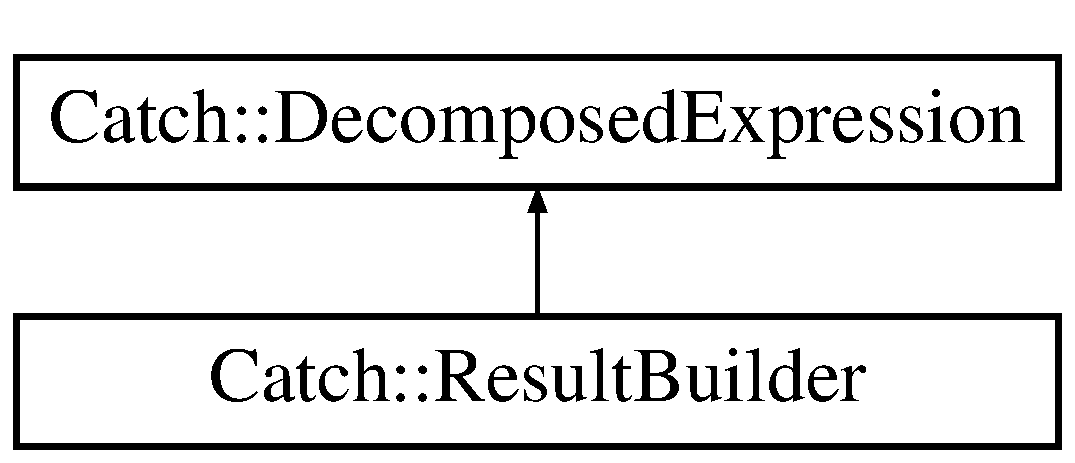
\includegraphics[height=2.000000cm]{classCatch_1_1ResultBuilder}
\end{center}
\end{figure}
\subsection*{Public Member Functions}
\begin{DoxyCompactItemize}
\item 
\hyperlink{classCatch_1_1ResultBuilder_a8579c3056f64f9324cf1181532828376}{Result\-Builder} (char const $\ast$macro\-Name, \hyperlink{structCatch_1_1SourceLineInfo}{Source\-Line\-Info} const \&line\-Info, char const $\ast$captured\-Expression, \hyperlink{structCatch_1_1ResultDisposition_a3396cad6e2259af326b3aae93e23e9d8}{Result\-Disposition\-::\-Flags} result\-Disposition, char const $\ast$second\-Arg=\char`\"{}\char`\"{})
\item 
\hyperlink{classCatch_1_1ResultBuilder_a687d1e9521d97f93c883ab070cc94c64}{$\sim$\-Result\-Builder} ()
\item 
{\footnotesize template$<$typename T $>$ }\\\hyperlink{classCatch_1_1ExpressionLhs}{Expression\-Lhs}$<$ T const \& $>$ \hyperlink{classCatch_1_1ResultBuilder_a1829db87e701758c4c520988883b25b5}{operator$<$=} (T const \&operand)
\item 
\hyperlink{classCatch_1_1ExpressionLhs}{Expression\-Lhs}$<$ bool $>$ \hyperlink{classCatch_1_1ResultBuilder_a3b87b20bcd1ef9e630880e59eeefba2a}{operator$<$=} (bool value)
\item 
{\footnotesize template$<$typename T $>$ }\\\hyperlink{classCatch_1_1ResultBuilder}{Result\-Builder} \& \hyperlink{classCatch_1_1ResultBuilder_a5aa79ce6160ab8cd800eb65bbd7a28a4}{operator$<$$<$} (T const \&value)
\item 
\hyperlink{classCatch_1_1ResultBuilder}{Result\-Builder} \& \hyperlink{classCatch_1_1ResultBuilder_af896e372db9d7fc90ddeceff3ad110d0}{set\-Result\-Type} (\hyperlink{structCatch_1_1ResultWas_a624e1ee3661fcf6094ceef1f654601ef}{Result\-Was\-::\-Of\-Type} result)
\item 
\hyperlink{classCatch_1_1ResultBuilder}{Result\-Builder} \& \hyperlink{classCatch_1_1ResultBuilder_ae504348b073d0360bfd5fc33347ec689}{set\-Result\-Type} (bool result)
\item 
void \hyperlink{classCatch_1_1ResultBuilder_a864e03b7300271de7cc44b9864463c5a}{end\-Expression} (\hyperlink{structCatch_1_1DecomposedExpression}{Decomposed\-Expression} const \&expr)
\item 
virtual void \hyperlink{classCatch_1_1ResultBuilder_a7d94b15cf04301a8617e7b16158b5d82}{reconstruct\-Expression} (std\-::string \&dest) const \hyperlink{catch_8hpp_a8ecdce4d3f57835f707915ae831eb847}{C\-A\-T\-C\-H\-\_\-\-O\-V\-E\-R\-R\-I\-D\-E}
\item 
\hyperlink{classCatch_1_1AssertionResult}{Assertion\-Result} \hyperlink{classCatch_1_1ResultBuilder_a31eba48feb02817d2151e31bd8331eeb}{build} () const 
\item 
\hyperlink{classCatch_1_1AssertionResult}{Assertion\-Result} \hyperlink{classCatch_1_1ResultBuilder_a606377d75e78899c90f94816ae8aff61}{build} (\hyperlink{structCatch_1_1DecomposedExpression}{Decomposed\-Expression} const \&expr) const 
\item 
void \hyperlink{classCatch_1_1ResultBuilder_a5bbd2f14a678f3e8d0f791ac6d233d65}{use\-Active\-Exception} (\hyperlink{structCatch_1_1ResultDisposition_a3396cad6e2259af326b3aae93e23e9d8}{Result\-Disposition\-::\-Flags} result\-Disposition=\hyperlink{structCatch_1_1ResultDisposition_a3396cad6e2259af326b3aae93e23e9d8af3bd52347ed6f8796e8ce2f77bb39ea5}{Result\-Disposition\-::\-Normal})
\item 
void \hyperlink{classCatch_1_1ResultBuilder_a10e467f7b7a4976e5d148b4d5066e8fd}{capture\-Result} (\hyperlink{structCatch_1_1ResultWas_a624e1ee3661fcf6094ceef1f654601ef}{Result\-Was\-::\-Of\-Type} result\-Type)
\item 
void \hyperlink{classCatch_1_1ResultBuilder_af2ae2343965802eeeb0abbd4ea9d2d36}{capture\-Expression} ()
\item 
void \hyperlink{classCatch_1_1ResultBuilder_a9ac96f6220c8dd8e4feee725c6228d77}{capture\-Expected\-Exception} (std\-::string const \&expected\-Message)
\item 
void \hyperlink{classCatch_1_1ResultBuilder_a2d6a194258f07f212fef098c0201038a}{capture\-Expected\-Exception} (\hyperlink{structCatch_1_1Matchers_1_1Impl_1_1MatcherBase}{Matchers\-::\-Impl\-::\-Matcher\-Base}$<$ std\-::string $>$ const \&matcher)
\item 
void \hyperlink{classCatch_1_1ResultBuilder_ad8bb17e4ac590b75bf8630d8f3502f4e}{handle\-Result} (\hyperlink{classCatch_1_1AssertionResult}{Assertion\-Result} const \&result)
\item 
void \hyperlink{classCatch_1_1ResultBuilder_a3085cdc46533d45bed6f652a2ac295c0}{react} ()
\item 
bool \hyperlink{classCatch_1_1ResultBuilder_a34cdbf7ad1e5b3cb4a94047f2d14bcb2}{should\-Debug\-Break} () const 
\item 
bool \hyperlink{classCatch_1_1ResultBuilder_a3dbf18a3a4b00173dab052a8864e435e}{allow\-Throws} () const 
\item 
{\footnotesize template$<$typename Arg\-T , typename Matcher\-T $>$ }\\void \hyperlink{classCatch_1_1ResultBuilder_a27425538bec8fee7ac69403c5df6078c}{capture\-Match} (Arg\-T const \&arg, Matcher\-T const \&matcher, char const $\ast$matcher\-String)
\item 
void \hyperlink{classCatch_1_1ResultBuilder_a87929808b4ec9b6cb5838edc1f27df17}{set\-Exception\-Guard} ()
\item 
void \hyperlink{classCatch_1_1ResultBuilder_a0990e93c1e13f96ffe02fa0f45e8f155}{unset\-Exception\-Guard} ()
\end{DoxyCompactItemize}


\subsection{Constructor \& Destructor Documentation}
\hypertarget{classCatch_1_1ResultBuilder_a8579c3056f64f9324cf1181532828376}{\index{Catch\-::\-Result\-Builder@{Catch\-::\-Result\-Builder}!Result\-Builder@{Result\-Builder}}
\index{Result\-Builder@{Result\-Builder}!Catch::ResultBuilder@{Catch\-::\-Result\-Builder}}
\subsubsection[{Result\-Builder}]{\setlength{\rightskip}{0pt plus 5cm}Catch\-::\-Result\-Builder\-::\-Result\-Builder (
\begin{DoxyParamCaption}
\item[{char const $\ast$}]{macro\-Name, }
\item[{{\bf Source\-Line\-Info} const \&}]{line\-Info, }
\item[{char const $\ast$}]{captured\-Expression, }
\item[{{\bf Result\-Disposition\-::\-Flags}}]{result\-Disposition, }
\item[{char const $\ast$}]{second\-Arg = {\ttfamily \char`\"{}\char`\"{}}}
\end{DoxyParamCaption}
)}}\label{classCatch_1_1ResultBuilder_a8579c3056f64f9324cf1181532828376}
\hypertarget{classCatch_1_1ResultBuilder_a687d1e9521d97f93c883ab070cc94c64}{\index{Catch\-::\-Result\-Builder@{Catch\-::\-Result\-Builder}!$\sim$\-Result\-Builder@{$\sim$\-Result\-Builder}}
\index{$\sim$\-Result\-Builder@{$\sim$\-Result\-Builder}!Catch::ResultBuilder@{Catch\-::\-Result\-Builder}}
\subsubsection[{$\sim$\-Result\-Builder}]{\setlength{\rightskip}{0pt plus 5cm}Catch\-::\-Result\-Builder\-::$\sim$\-Result\-Builder (
\begin{DoxyParamCaption}
{}
\end{DoxyParamCaption}
)}}\label{classCatch_1_1ResultBuilder_a687d1e9521d97f93c883ab070cc94c64}


\subsection{Member Function Documentation}
\hypertarget{classCatch_1_1ResultBuilder_a3dbf18a3a4b00173dab052a8864e435e}{\index{Catch\-::\-Result\-Builder@{Catch\-::\-Result\-Builder}!allow\-Throws@{allow\-Throws}}
\index{allow\-Throws@{allow\-Throws}!Catch::ResultBuilder@{Catch\-::\-Result\-Builder}}
\subsubsection[{allow\-Throws}]{\setlength{\rightskip}{0pt plus 5cm}bool Catch\-::\-Result\-Builder\-::allow\-Throws (
\begin{DoxyParamCaption}
{}
\end{DoxyParamCaption}
) const}}\label{classCatch_1_1ResultBuilder_a3dbf18a3a4b00173dab052a8864e435e}
\hypertarget{classCatch_1_1ResultBuilder_a31eba48feb02817d2151e31bd8331eeb}{\index{Catch\-::\-Result\-Builder@{Catch\-::\-Result\-Builder}!build@{build}}
\index{build@{build}!Catch::ResultBuilder@{Catch\-::\-Result\-Builder}}
\subsubsection[{build}]{\setlength{\rightskip}{0pt plus 5cm}{\bf Assertion\-Result} Catch\-::\-Result\-Builder\-::build (
\begin{DoxyParamCaption}
{}
\end{DoxyParamCaption}
) const}}\label{classCatch_1_1ResultBuilder_a31eba48feb02817d2151e31bd8331eeb}
\hypertarget{classCatch_1_1ResultBuilder_a606377d75e78899c90f94816ae8aff61}{\index{Catch\-::\-Result\-Builder@{Catch\-::\-Result\-Builder}!build@{build}}
\index{build@{build}!Catch::ResultBuilder@{Catch\-::\-Result\-Builder}}
\subsubsection[{build}]{\setlength{\rightskip}{0pt plus 5cm}{\bf Assertion\-Result} Catch\-::\-Result\-Builder\-::build (
\begin{DoxyParamCaption}
\item[{{\bf Decomposed\-Expression} const \&}]{expr}
\end{DoxyParamCaption}
) const}}\label{classCatch_1_1ResultBuilder_a606377d75e78899c90f94816ae8aff61}
\hypertarget{classCatch_1_1ResultBuilder_a9ac96f6220c8dd8e4feee725c6228d77}{\index{Catch\-::\-Result\-Builder@{Catch\-::\-Result\-Builder}!capture\-Expected\-Exception@{capture\-Expected\-Exception}}
\index{capture\-Expected\-Exception@{capture\-Expected\-Exception}!Catch::ResultBuilder@{Catch\-::\-Result\-Builder}}
\subsubsection[{capture\-Expected\-Exception}]{\setlength{\rightskip}{0pt plus 5cm}void Catch\-::\-Result\-Builder\-::capture\-Expected\-Exception (
\begin{DoxyParamCaption}
\item[{std\-::string const \&}]{expected\-Message}
\end{DoxyParamCaption}
)}}\label{classCatch_1_1ResultBuilder_a9ac96f6220c8dd8e4feee725c6228d77}
\hypertarget{classCatch_1_1ResultBuilder_a2d6a194258f07f212fef098c0201038a}{\index{Catch\-::\-Result\-Builder@{Catch\-::\-Result\-Builder}!capture\-Expected\-Exception@{capture\-Expected\-Exception}}
\index{capture\-Expected\-Exception@{capture\-Expected\-Exception}!Catch::ResultBuilder@{Catch\-::\-Result\-Builder}}
\subsubsection[{capture\-Expected\-Exception}]{\setlength{\rightskip}{0pt plus 5cm}void Catch\-::\-Result\-Builder\-::capture\-Expected\-Exception (
\begin{DoxyParamCaption}
\item[{{\bf Matchers\-::\-Impl\-::\-Matcher\-Base}$<$ std\-::string $>$ const \&}]{matcher}
\end{DoxyParamCaption}
)}}\label{classCatch_1_1ResultBuilder_a2d6a194258f07f212fef098c0201038a}
\hypertarget{classCatch_1_1ResultBuilder_af2ae2343965802eeeb0abbd4ea9d2d36}{\index{Catch\-::\-Result\-Builder@{Catch\-::\-Result\-Builder}!capture\-Expression@{capture\-Expression}}
\index{capture\-Expression@{capture\-Expression}!Catch::ResultBuilder@{Catch\-::\-Result\-Builder}}
\subsubsection[{capture\-Expression}]{\setlength{\rightskip}{0pt plus 5cm}void Catch\-::\-Result\-Builder\-::capture\-Expression (
\begin{DoxyParamCaption}
{}
\end{DoxyParamCaption}
)}}\label{classCatch_1_1ResultBuilder_af2ae2343965802eeeb0abbd4ea9d2d36}
\hypertarget{classCatch_1_1ResultBuilder_a27425538bec8fee7ac69403c5df6078c}{\index{Catch\-::\-Result\-Builder@{Catch\-::\-Result\-Builder}!capture\-Match@{capture\-Match}}
\index{capture\-Match@{capture\-Match}!Catch::ResultBuilder@{Catch\-::\-Result\-Builder}}
\subsubsection[{capture\-Match}]{\setlength{\rightskip}{0pt plus 5cm}template$<$typename Arg\-T , typename Matcher\-T $>$ void Catch\-::\-Result\-Builder\-::capture\-Match (
\begin{DoxyParamCaption}
\item[{Arg\-T const \&}]{arg, }
\item[{Matcher\-T const \&}]{matcher, }
\item[{char const $\ast$}]{matcher\-String}
\end{DoxyParamCaption}
)\hspace{0.3cm}{\ttfamily [inline]}}}\label{classCatch_1_1ResultBuilder_a27425538bec8fee7ac69403c5df6078c}
\hypertarget{classCatch_1_1ResultBuilder_a10e467f7b7a4976e5d148b4d5066e8fd}{\index{Catch\-::\-Result\-Builder@{Catch\-::\-Result\-Builder}!capture\-Result@{capture\-Result}}
\index{capture\-Result@{capture\-Result}!Catch::ResultBuilder@{Catch\-::\-Result\-Builder}}
\subsubsection[{capture\-Result}]{\setlength{\rightskip}{0pt plus 5cm}void Catch\-::\-Result\-Builder\-::capture\-Result (
\begin{DoxyParamCaption}
\item[{{\bf Result\-Was\-::\-Of\-Type}}]{result\-Type}
\end{DoxyParamCaption}
)}}\label{classCatch_1_1ResultBuilder_a10e467f7b7a4976e5d148b4d5066e8fd}
\hypertarget{classCatch_1_1ResultBuilder_a864e03b7300271de7cc44b9864463c5a}{\index{Catch\-::\-Result\-Builder@{Catch\-::\-Result\-Builder}!end\-Expression@{end\-Expression}}
\index{end\-Expression@{end\-Expression}!Catch::ResultBuilder@{Catch\-::\-Result\-Builder}}
\subsubsection[{end\-Expression}]{\setlength{\rightskip}{0pt plus 5cm}void Catch\-::\-Result\-Builder\-::end\-Expression (
\begin{DoxyParamCaption}
\item[{{\bf Decomposed\-Expression} const \&}]{expr}
\end{DoxyParamCaption}
)}}\label{classCatch_1_1ResultBuilder_a864e03b7300271de7cc44b9864463c5a}
\hypertarget{classCatch_1_1ResultBuilder_ad8bb17e4ac590b75bf8630d8f3502f4e}{\index{Catch\-::\-Result\-Builder@{Catch\-::\-Result\-Builder}!handle\-Result@{handle\-Result}}
\index{handle\-Result@{handle\-Result}!Catch::ResultBuilder@{Catch\-::\-Result\-Builder}}
\subsubsection[{handle\-Result}]{\setlength{\rightskip}{0pt plus 5cm}void Catch\-::\-Result\-Builder\-::handle\-Result (
\begin{DoxyParamCaption}
\item[{{\bf Assertion\-Result} const \&}]{result}
\end{DoxyParamCaption}
)}}\label{classCatch_1_1ResultBuilder_ad8bb17e4ac590b75bf8630d8f3502f4e}
\hypertarget{classCatch_1_1ResultBuilder_a5aa79ce6160ab8cd800eb65bbd7a28a4}{\index{Catch\-::\-Result\-Builder@{Catch\-::\-Result\-Builder}!operator$<$$<$@{operator$<$$<$}}
\index{operator$<$$<$@{operator$<$$<$}!Catch::ResultBuilder@{Catch\-::\-Result\-Builder}}
\subsubsection[{operator$<$$<$}]{\setlength{\rightskip}{0pt plus 5cm}template$<$typename T $>$ {\bf Result\-Builder}\& Catch\-::\-Result\-Builder\-::operator$<$$<$ (
\begin{DoxyParamCaption}
\item[{T const \&}]{value}
\end{DoxyParamCaption}
)\hspace{0.3cm}{\ttfamily [inline]}}}\label{classCatch_1_1ResultBuilder_a5aa79ce6160ab8cd800eb65bbd7a28a4}
\hypertarget{classCatch_1_1ResultBuilder_a3b87b20bcd1ef9e630880e59eeefba2a}{\index{Catch\-::\-Result\-Builder@{Catch\-::\-Result\-Builder}!operator$<$=@{operator$<$=}}
\index{operator$<$=@{operator$<$=}!Catch::ResultBuilder@{Catch\-::\-Result\-Builder}}
\subsubsection[{operator$<$=}]{\setlength{\rightskip}{0pt plus 5cm}{\bf Expression\-Lhs}$<$ bool $>$ Catch\-::\-Result\-Builder\-::operator$<$= (
\begin{DoxyParamCaption}
\item[{bool}]{value}
\end{DoxyParamCaption}
)\hspace{0.3cm}{\ttfamily [inline]}}}\label{classCatch_1_1ResultBuilder_a3b87b20bcd1ef9e630880e59eeefba2a}
\hypertarget{classCatch_1_1ResultBuilder_a1829db87e701758c4c520988883b25b5}{\index{Catch\-::\-Result\-Builder@{Catch\-::\-Result\-Builder}!operator$<$=@{operator$<$=}}
\index{operator$<$=@{operator$<$=}!Catch::ResultBuilder@{Catch\-::\-Result\-Builder}}
\subsubsection[{operator$<$=}]{\setlength{\rightskip}{0pt plus 5cm}template$<$typename T $>$ {\bf Expression\-Lhs}$<$ T const \& $>$ Catch\-::\-Result\-Builder\-::operator$<$= (
\begin{DoxyParamCaption}
\item[{T const \&}]{operand}
\end{DoxyParamCaption}
)\hspace{0.3cm}{\ttfamily [inline]}}}\label{classCatch_1_1ResultBuilder_a1829db87e701758c4c520988883b25b5}
\hypertarget{classCatch_1_1ResultBuilder_a3085cdc46533d45bed6f652a2ac295c0}{\index{Catch\-::\-Result\-Builder@{Catch\-::\-Result\-Builder}!react@{react}}
\index{react@{react}!Catch::ResultBuilder@{Catch\-::\-Result\-Builder}}
\subsubsection[{react}]{\setlength{\rightskip}{0pt plus 5cm}void Catch\-::\-Result\-Builder\-::react (
\begin{DoxyParamCaption}
{}
\end{DoxyParamCaption}
)}}\label{classCatch_1_1ResultBuilder_a3085cdc46533d45bed6f652a2ac295c0}
\hypertarget{classCatch_1_1ResultBuilder_a7d94b15cf04301a8617e7b16158b5d82}{\index{Catch\-::\-Result\-Builder@{Catch\-::\-Result\-Builder}!reconstruct\-Expression@{reconstruct\-Expression}}
\index{reconstruct\-Expression@{reconstruct\-Expression}!Catch::ResultBuilder@{Catch\-::\-Result\-Builder}}
\subsubsection[{reconstruct\-Expression}]{\setlength{\rightskip}{0pt plus 5cm}virtual void Catch\-::\-Result\-Builder\-::reconstruct\-Expression (
\begin{DoxyParamCaption}
\item[{std\-::string \&}]{dest}
\end{DoxyParamCaption}
) const\hspace{0.3cm}{\ttfamily [virtual]}}}\label{classCatch_1_1ResultBuilder_a7d94b15cf04301a8617e7b16158b5d82}


Implements \hyperlink{structCatch_1_1DecomposedExpression_a9ce7f356dc96f11f80e40c82f5aa7e55}{Catch\-::\-Decomposed\-Expression}.

\hypertarget{classCatch_1_1ResultBuilder_a87929808b4ec9b6cb5838edc1f27df17}{\index{Catch\-::\-Result\-Builder@{Catch\-::\-Result\-Builder}!set\-Exception\-Guard@{set\-Exception\-Guard}}
\index{set\-Exception\-Guard@{set\-Exception\-Guard}!Catch::ResultBuilder@{Catch\-::\-Result\-Builder}}
\subsubsection[{set\-Exception\-Guard}]{\setlength{\rightskip}{0pt plus 5cm}void Catch\-::\-Result\-Builder\-::set\-Exception\-Guard (
\begin{DoxyParamCaption}
{}
\end{DoxyParamCaption}
)}}\label{classCatch_1_1ResultBuilder_a87929808b4ec9b6cb5838edc1f27df17}
\hypertarget{classCatch_1_1ResultBuilder_af896e372db9d7fc90ddeceff3ad110d0}{\index{Catch\-::\-Result\-Builder@{Catch\-::\-Result\-Builder}!set\-Result\-Type@{set\-Result\-Type}}
\index{set\-Result\-Type@{set\-Result\-Type}!Catch::ResultBuilder@{Catch\-::\-Result\-Builder}}
\subsubsection[{set\-Result\-Type}]{\setlength{\rightskip}{0pt plus 5cm}{\bf Result\-Builder}\& Catch\-::\-Result\-Builder\-::set\-Result\-Type (
\begin{DoxyParamCaption}
\item[{{\bf Result\-Was\-::\-Of\-Type}}]{result}
\end{DoxyParamCaption}
)}}\label{classCatch_1_1ResultBuilder_af896e372db9d7fc90ddeceff3ad110d0}
\hypertarget{classCatch_1_1ResultBuilder_ae504348b073d0360bfd5fc33347ec689}{\index{Catch\-::\-Result\-Builder@{Catch\-::\-Result\-Builder}!set\-Result\-Type@{set\-Result\-Type}}
\index{set\-Result\-Type@{set\-Result\-Type}!Catch::ResultBuilder@{Catch\-::\-Result\-Builder}}
\subsubsection[{set\-Result\-Type}]{\setlength{\rightskip}{0pt plus 5cm}{\bf Result\-Builder}\& Catch\-::\-Result\-Builder\-::set\-Result\-Type (
\begin{DoxyParamCaption}
\item[{bool}]{result}
\end{DoxyParamCaption}
)}}\label{classCatch_1_1ResultBuilder_ae504348b073d0360bfd5fc33347ec689}
\hypertarget{classCatch_1_1ResultBuilder_a34cdbf7ad1e5b3cb4a94047f2d14bcb2}{\index{Catch\-::\-Result\-Builder@{Catch\-::\-Result\-Builder}!should\-Debug\-Break@{should\-Debug\-Break}}
\index{should\-Debug\-Break@{should\-Debug\-Break}!Catch::ResultBuilder@{Catch\-::\-Result\-Builder}}
\subsubsection[{should\-Debug\-Break}]{\setlength{\rightskip}{0pt plus 5cm}bool Catch\-::\-Result\-Builder\-::should\-Debug\-Break (
\begin{DoxyParamCaption}
{}
\end{DoxyParamCaption}
) const}}\label{classCatch_1_1ResultBuilder_a34cdbf7ad1e5b3cb4a94047f2d14bcb2}
\hypertarget{classCatch_1_1ResultBuilder_a0990e93c1e13f96ffe02fa0f45e8f155}{\index{Catch\-::\-Result\-Builder@{Catch\-::\-Result\-Builder}!unset\-Exception\-Guard@{unset\-Exception\-Guard}}
\index{unset\-Exception\-Guard@{unset\-Exception\-Guard}!Catch::ResultBuilder@{Catch\-::\-Result\-Builder}}
\subsubsection[{unset\-Exception\-Guard}]{\setlength{\rightskip}{0pt plus 5cm}void Catch\-::\-Result\-Builder\-::unset\-Exception\-Guard (
\begin{DoxyParamCaption}
{}
\end{DoxyParamCaption}
)}}\label{classCatch_1_1ResultBuilder_a0990e93c1e13f96ffe02fa0f45e8f155}
\hypertarget{classCatch_1_1ResultBuilder_a5bbd2f14a678f3e8d0f791ac6d233d65}{\index{Catch\-::\-Result\-Builder@{Catch\-::\-Result\-Builder}!use\-Active\-Exception@{use\-Active\-Exception}}
\index{use\-Active\-Exception@{use\-Active\-Exception}!Catch::ResultBuilder@{Catch\-::\-Result\-Builder}}
\subsubsection[{use\-Active\-Exception}]{\setlength{\rightskip}{0pt plus 5cm}void Catch\-::\-Result\-Builder\-::use\-Active\-Exception (
\begin{DoxyParamCaption}
\item[{{\bf Result\-Disposition\-::\-Flags}}]{result\-Disposition = {\ttfamily {\bf Result\-Disposition\-::\-Normal}}}
\end{DoxyParamCaption}
)}}\label{classCatch_1_1ResultBuilder_a5bbd2f14a678f3e8d0f791ac6d233d65}


The documentation for this class was generated from the following file\-:\begin{DoxyCompactItemize}
\item 
/home/alexander/\-Un\-B/\-M\-P/\-Trabalho\-\_\-2\-\_\-\-M\-P\-\_\-\-Alexander\-\_\-13\-\_\-0039853/include/\hyperlink{catch_8hpp}{catch.\-hpp}\end{DoxyCompactItemize}

\hypertarget{structCatch_1_1ResultDisposition}{\section{Catch\-:\-:Result\-Disposition Struct Reference}
\label{structCatch_1_1ResultDisposition}\index{Catch\-::\-Result\-Disposition@{Catch\-::\-Result\-Disposition}}
}


{\ttfamily \#include $<$catch.\-hpp$>$}

\subsection*{Public Types}
\begin{DoxyCompactItemize}
\item 
enum \hyperlink{structCatch_1_1ResultDisposition_a3396cad6e2259af326b3aae93e23e9d8}{Flags} \{ \hyperlink{structCatch_1_1ResultDisposition_a3396cad6e2259af326b3aae93e23e9d8af3bd52347ed6f8796e8ce2f77bb39ea5}{Normal} = 0x01, 
\hyperlink{structCatch_1_1ResultDisposition_a3396cad6e2259af326b3aae93e23e9d8aa18c94bd60c5614e17a84c2ced3bbfd5}{Continue\-On\-Failure} = 0x02, 
\hyperlink{structCatch_1_1ResultDisposition_a3396cad6e2259af326b3aae93e23e9d8a9980604245f19884691f941dec03eeb8}{False\-Test} = 0x04, 
\hyperlink{structCatch_1_1ResultDisposition_a3396cad6e2259af326b3aae93e23e9d8a1a88eb6004bddee4ccae4b421991bf54}{Suppress\-Fail} = 0x08
 \}
\end{DoxyCompactItemize}


\subsection{Member Enumeration Documentation}
\hypertarget{structCatch_1_1ResultDisposition_a3396cad6e2259af326b3aae93e23e9d8}{\index{Catch\-::\-Result\-Disposition@{Catch\-::\-Result\-Disposition}!Flags@{Flags}}
\index{Flags@{Flags}!Catch::ResultDisposition@{Catch\-::\-Result\-Disposition}}
\subsubsection[{Flags}]{\setlength{\rightskip}{0pt plus 5cm}enum {\bf Catch\-::\-Result\-Disposition\-::\-Flags}}}\label{structCatch_1_1ResultDisposition_a3396cad6e2259af326b3aae93e23e9d8}
\begin{Desc}
\item[Enumerator]\par
\begin{description}
\index{Normal@{Normal}!Catch\-::\-Result\-Disposition@{Catch\-::\-Result\-Disposition}}\index{Catch\-::\-Result\-Disposition@{Catch\-::\-Result\-Disposition}!Normal@{Normal}}\item[{\em 
\hypertarget{structCatch_1_1ResultDisposition_a3396cad6e2259af326b3aae93e23e9d8af3bd52347ed6f8796e8ce2f77bb39ea5}{Normal}\label{structCatch_1_1ResultDisposition_a3396cad6e2259af326b3aae93e23e9d8af3bd52347ed6f8796e8ce2f77bb39ea5}
}]\index{Continue\-On\-Failure@{Continue\-On\-Failure}!Catch\-::\-Result\-Disposition@{Catch\-::\-Result\-Disposition}}\index{Catch\-::\-Result\-Disposition@{Catch\-::\-Result\-Disposition}!Continue\-On\-Failure@{Continue\-On\-Failure}}\item[{\em 
\hypertarget{structCatch_1_1ResultDisposition_a3396cad6e2259af326b3aae93e23e9d8aa18c94bd60c5614e17a84c2ced3bbfd5}{Continue\-On\-Failure}\label{structCatch_1_1ResultDisposition_a3396cad6e2259af326b3aae93e23e9d8aa18c94bd60c5614e17a84c2ced3bbfd5}
}]\index{False\-Test@{False\-Test}!Catch\-::\-Result\-Disposition@{Catch\-::\-Result\-Disposition}}\index{Catch\-::\-Result\-Disposition@{Catch\-::\-Result\-Disposition}!False\-Test@{False\-Test}}\item[{\em 
\hypertarget{structCatch_1_1ResultDisposition_a3396cad6e2259af326b3aae93e23e9d8a9980604245f19884691f941dec03eeb8}{False\-Test}\label{structCatch_1_1ResultDisposition_a3396cad6e2259af326b3aae93e23e9d8a9980604245f19884691f941dec03eeb8}
}]\index{Suppress\-Fail@{Suppress\-Fail}!Catch\-::\-Result\-Disposition@{Catch\-::\-Result\-Disposition}}\index{Catch\-::\-Result\-Disposition@{Catch\-::\-Result\-Disposition}!Suppress\-Fail@{Suppress\-Fail}}\item[{\em 
\hypertarget{structCatch_1_1ResultDisposition_a3396cad6e2259af326b3aae93e23e9d8a1a88eb6004bddee4ccae4b421991bf54}{Suppress\-Fail}\label{structCatch_1_1ResultDisposition_a3396cad6e2259af326b3aae93e23e9d8a1a88eb6004bddee4ccae4b421991bf54}
}]\end{description}
\end{Desc}


The documentation for this struct was generated from the following file\-:\begin{DoxyCompactItemize}
\item 
/home/alexander/\-Un\-B/\-M\-P/\-Trabalho\-\_\-2\-\_\-\-M\-P\-\_\-\-Alexander\-\_\-13\-\_\-0039853/include/\hyperlink{catch_8hpp}{catch.\-hpp}\end{DoxyCompactItemize}

\hypertarget{structCatch_1_1ResultWas}{\section{Catch\-:\-:Result\-Was Struct Reference}
\label{structCatch_1_1ResultWas}\index{Catch\-::\-Result\-Was@{Catch\-::\-Result\-Was}}
}


{\ttfamily \#include $<$catch.\-hpp$>$}

\subsection*{Public Types}
\begin{DoxyCompactItemize}
\item 
enum \hyperlink{structCatch_1_1ResultWas_a624e1ee3661fcf6094ceef1f654601ef}{Of\-Type} \{ \\*
\hyperlink{structCatch_1_1ResultWas_a624e1ee3661fcf6094ceef1f654601efa65721dda02fe5efb522e7449e496608a}{Unknown} = -\/1, 
\hyperlink{structCatch_1_1ResultWas_a624e1ee3661fcf6094ceef1f654601efae7cbe89bb9ec7ece9b44d48b63d01b63}{Ok} = 0, 
\hyperlink{structCatch_1_1ResultWas_a624e1ee3661fcf6094ceef1f654601efa30222063929ca1b6318faa78e8242f1c}{Info} = 1, 
\hyperlink{structCatch_1_1ResultWas_a624e1ee3661fcf6094ceef1f654601efa67e9d36ba0f04a60a19896834d840c21}{Warning} = 2, 
\\*
\hyperlink{structCatch_1_1ResultWas_a624e1ee3661fcf6094ceef1f654601efa1818f1b198f10b5734c405142b22025c}{Failure\-Bit} = 0x10, 
\hyperlink{structCatch_1_1ResultWas_a624e1ee3661fcf6094ceef1f654601efa5e7126b8458dc1376ac870a719f7873f}{Expression\-Failed} = Failure\-Bit $\vert$ 1, 
\hyperlink{structCatch_1_1ResultWas_a624e1ee3661fcf6094ceef1f654601efacecfc052e2499499b13304249303cc36}{Explicit\-Failure} = Failure\-Bit $\vert$ 2, 
\hyperlink{structCatch_1_1ResultWas_a624e1ee3661fcf6094ceef1f654601efaa9107b7836cc7590ca668002f76d27c7}{Exception} = 0x100 $\vert$ Failure\-Bit, 
\\*
\hyperlink{structCatch_1_1ResultWas_a624e1ee3661fcf6094ceef1f654601efa3bb56296483947280cf7fa1ad074ab45}{Threw\-Exception} = Exception $\vert$ 1, 
\hyperlink{structCatch_1_1ResultWas_a624e1ee3661fcf6094ceef1f654601efa8b6d3d5bc78d4e7a95543b6ecfbdb57d}{Didnt\-Throw\-Exception} = Exception $\vert$ 2, 
\hyperlink{structCatch_1_1ResultWas_a624e1ee3661fcf6094ceef1f654601efa87fa1f2a2a63290b61948002e2935377}{Fatal\-Error\-Condition} = 0x200 $\vert$ Failure\-Bit
 \}
\end{DoxyCompactItemize}


\subsection{Member Enumeration Documentation}
\hypertarget{structCatch_1_1ResultWas_a624e1ee3661fcf6094ceef1f654601ef}{\index{Catch\-::\-Result\-Was@{Catch\-::\-Result\-Was}!Of\-Type@{Of\-Type}}
\index{Of\-Type@{Of\-Type}!Catch::ResultWas@{Catch\-::\-Result\-Was}}
\subsubsection[{Of\-Type}]{\setlength{\rightskip}{0pt plus 5cm}enum {\bf Catch\-::\-Result\-Was\-::\-Of\-Type}}}\label{structCatch_1_1ResultWas_a624e1ee3661fcf6094ceef1f654601ef}
\begin{Desc}
\item[Enumerator]\par
\begin{description}
\index{Unknown@{Unknown}!Catch\-::\-Result\-Was@{Catch\-::\-Result\-Was}}\index{Catch\-::\-Result\-Was@{Catch\-::\-Result\-Was}!Unknown@{Unknown}}\item[{\em 
\hypertarget{structCatch_1_1ResultWas_a624e1ee3661fcf6094ceef1f654601efa65721dda02fe5efb522e7449e496608a}{Unknown}\label{structCatch_1_1ResultWas_a624e1ee3661fcf6094ceef1f654601efa65721dda02fe5efb522e7449e496608a}
}]\index{Ok@{Ok}!Catch\-::\-Result\-Was@{Catch\-::\-Result\-Was}}\index{Catch\-::\-Result\-Was@{Catch\-::\-Result\-Was}!Ok@{Ok}}\item[{\em 
\hypertarget{structCatch_1_1ResultWas_a624e1ee3661fcf6094ceef1f654601efae7cbe89bb9ec7ece9b44d48b63d01b63}{Ok}\label{structCatch_1_1ResultWas_a624e1ee3661fcf6094ceef1f654601efae7cbe89bb9ec7ece9b44d48b63d01b63}
}]\index{Info@{Info}!Catch\-::\-Result\-Was@{Catch\-::\-Result\-Was}}\index{Catch\-::\-Result\-Was@{Catch\-::\-Result\-Was}!Info@{Info}}\item[{\em 
\hypertarget{structCatch_1_1ResultWas_a624e1ee3661fcf6094ceef1f654601efa30222063929ca1b6318faa78e8242f1c}{Info}\label{structCatch_1_1ResultWas_a624e1ee3661fcf6094ceef1f654601efa30222063929ca1b6318faa78e8242f1c}
}]\index{Warning@{Warning}!Catch\-::\-Result\-Was@{Catch\-::\-Result\-Was}}\index{Catch\-::\-Result\-Was@{Catch\-::\-Result\-Was}!Warning@{Warning}}\item[{\em 
\hypertarget{structCatch_1_1ResultWas_a624e1ee3661fcf6094ceef1f654601efa67e9d36ba0f04a60a19896834d840c21}{Warning}\label{structCatch_1_1ResultWas_a624e1ee3661fcf6094ceef1f654601efa67e9d36ba0f04a60a19896834d840c21}
}]\index{Failure\-Bit@{Failure\-Bit}!Catch\-::\-Result\-Was@{Catch\-::\-Result\-Was}}\index{Catch\-::\-Result\-Was@{Catch\-::\-Result\-Was}!Failure\-Bit@{Failure\-Bit}}\item[{\em 
\hypertarget{structCatch_1_1ResultWas_a624e1ee3661fcf6094ceef1f654601efa1818f1b198f10b5734c405142b22025c}{Failure\-Bit}\label{structCatch_1_1ResultWas_a624e1ee3661fcf6094ceef1f654601efa1818f1b198f10b5734c405142b22025c}
}]\index{Expression\-Failed@{Expression\-Failed}!Catch\-::\-Result\-Was@{Catch\-::\-Result\-Was}}\index{Catch\-::\-Result\-Was@{Catch\-::\-Result\-Was}!Expression\-Failed@{Expression\-Failed}}\item[{\em 
\hypertarget{structCatch_1_1ResultWas_a624e1ee3661fcf6094ceef1f654601efa5e7126b8458dc1376ac870a719f7873f}{Expression\-Failed}\label{structCatch_1_1ResultWas_a624e1ee3661fcf6094ceef1f654601efa5e7126b8458dc1376ac870a719f7873f}
}]\index{Explicit\-Failure@{Explicit\-Failure}!Catch\-::\-Result\-Was@{Catch\-::\-Result\-Was}}\index{Catch\-::\-Result\-Was@{Catch\-::\-Result\-Was}!Explicit\-Failure@{Explicit\-Failure}}\item[{\em 
\hypertarget{structCatch_1_1ResultWas_a624e1ee3661fcf6094ceef1f654601efacecfc052e2499499b13304249303cc36}{Explicit\-Failure}\label{structCatch_1_1ResultWas_a624e1ee3661fcf6094ceef1f654601efacecfc052e2499499b13304249303cc36}
}]\index{Exception@{Exception}!Catch\-::\-Result\-Was@{Catch\-::\-Result\-Was}}\index{Catch\-::\-Result\-Was@{Catch\-::\-Result\-Was}!Exception@{Exception}}\item[{\em 
\hypertarget{structCatch_1_1ResultWas_a624e1ee3661fcf6094ceef1f654601efaa9107b7836cc7590ca668002f76d27c7}{Exception}\label{structCatch_1_1ResultWas_a624e1ee3661fcf6094ceef1f654601efaa9107b7836cc7590ca668002f76d27c7}
}]\index{Threw\-Exception@{Threw\-Exception}!Catch\-::\-Result\-Was@{Catch\-::\-Result\-Was}}\index{Catch\-::\-Result\-Was@{Catch\-::\-Result\-Was}!Threw\-Exception@{Threw\-Exception}}\item[{\em 
\hypertarget{structCatch_1_1ResultWas_a624e1ee3661fcf6094ceef1f654601efa3bb56296483947280cf7fa1ad074ab45}{Threw\-Exception}\label{structCatch_1_1ResultWas_a624e1ee3661fcf6094ceef1f654601efa3bb56296483947280cf7fa1ad074ab45}
}]\index{Didnt\-Throw\-Exception@{Didnt\-Throw\-Exception}!Catch\-::\-Result\-Was@{Catch\-::\-Result\-Was}}\index{Catch\-::\-Result\-Was@{Catch\-::\-Result\-Was}!Didnt\-Throw\-Exception@{Didnt\-Throw\-Exception}}\item[{\em 
\hypertarget{structCatch_1_1ResultWas_a624e1ee3661fcf6094ceef1f654601efa8b6d3d5bc78d4e7a95543b6ecfbdb57d}{Didnt\-Throw\-Exception}\label{structCatch_1_1ResultWas_a624e1ee3661fcf6094ceef1f654601efa8b6d3d5bc78d4e7a95543b6ecfbdb57d}
}]\index{Fatal\-Error\-Condition@{Fatal\-Error\-Condition}!Catch\-::\-Result\-Was@{Catch\-::\-Result\-Was}}\index{Catch\-::\-Result\-Was@{Catch\-::\-Result\-Was}!Fatal\-Error\-Condition@{Fatal\-Error\-Condition}}\item[{\em 
\hypertarget{structCatch_1_1ResultWas_a624e1ee3661fcf6094ceef1f654601efa87fa1f2a2a63290b61948002e2935377}{Fatal\-Error\-Condition}\label{structCatch_1_1ResultWas_a624e1ee3661fcf6094ceef1f654601efa87fa1f2a2a63290b61948002e2935377}
}]\end{description}
\end{Desc}


The documentation for this struct was generated from the following file\-:\begin{DoxyCompactItemize}
\item 
/home/alexander/\-Un\-B/\-M\-P/\-Trabalho\-\_\-2\-\_\-\-M\-P\-\_\-\-Alexander\-\_\-13\-\_\-0039853/include/\hyperlink{catch_8hpp}{catch.\-hpp}\end{DoxyCompactItemize}

\hypertarget{classCatch_1_1SafeBool}{\section{Catch\-:\-:Safe\-Bool Class Reference}
\label{classCatch_1_1SafeBool}\index{Catch\-::\-Safe\-Bool@{Catch\-::\-Safe\-Bool}}
}


{\ttfamily \#include $<$catch.\-hpp$>$}

\subsection*{Public Types}
\begin{DoxyCompactItemize}
\item 
typedef void(Safe\-Bool\-::$\ast$ \hyperlink{classCatch_1_1SafeBool_a14cd49eced5b255a1f59512d3b9395ae}{type} )() const 
\end{DoxyCompactItemize}
\subsection*{Static Public Member Functions}
\begin{DoxyCompactItemize}
\item 
static \hyperlink{classCatch_1_1SafeBool_a14cd49eced5b255a1f59512d3b9395ae}{type} \hyperlink{classCatch_1_1SafeBool_af0ea63d9820f8bf7a8b76377913c4e77}{make\-Safe} (bool value)
\end{DoxyCompactItemize}


\subsection{Member Typedef Documentation}
\hypertarget{classCatch_1_1SafeBool_a14cd49eced5b255a1f59512d3b9395ae}{\index{Catch\-::\-Safe\-Bool@{Catch\-::\-Safe\-Bool}!type@{type}}
\index{type@{type}!Catch::SafeBool@{Catch\-::\-Safe\-Bool}}
\subsubsection[{type}]{\setlength{\rightskip}{0pt plus 5cm}typedef void(Safe\-Bool\-::$\ast$ Catch\-::\-Safe\-Bool\-::type)() const }}\label{classCatch_1_1SafeBool_a14cd49eced5b255a1f59512d3b9395ae}


\subsection{Member Function Documentation}
\hypertarget{classCatch_1_1SafeBool_af0ea63d9820f8bf7a8b76377913c4e77}{\index{Catch\-::\-Safe\-Bool@{Catch\-::\-Safe\-Bool}!make\-Safe@{make\-Safe}}
\index{make\-Safe@{make\-Safe}!Catch::SafeBool@{Catch\-::\-Safe\-Bool}}
\subsubsection[{make\-Safe}]{\setlength{\rightskip}{0pt plus 5cm}static {\bf type} Catch\-::\-Safe\-Bool\-::make\-Safe (
\begin{DoxyParamCaption}
\item[{bool}]{value}
\end{DoxyParamCaption}
)\hspace{0.3cm}{\ttfamily [inline]}, {\ttfamily [static]}}}\label{classCatch_1_1SafeBool_af0ea63d9820f8bf7a8b76377913c4e77}


The documentation for this class was generated from the following file\-:\begin{DoxyCompactItemize}
\item 
/home/alexander/\-Un\-B/\-M\-P/\-Trabalho\-\_\-2\-\_\-\-M\-P\-\_\-\-Alexander\-\_\-13\-\_\-0039853/include/\hyperlink{catch_8hpp}{catch.\-hpp}\end{DoxyCompactItemize}

\hypertarget{classCatch_1_1ScopedMessage}{\section{Catch\-:\-:Scoped\-Message Class Reference}
\label{classCatch_1_1ScopedMessage}\index{Catch\-::\-Scoped\-Message@{Catch\-::\-Scoped\-Message}}
}


{\ttfamily \#include $<$catch.\-hpp$>$}

\subsection*{Public Member Functions}
\begin{DoxyCompactItemize}
\item 
\hyperlink{classCatch_1_1ScopedMessage_a5cc59f0f2ebe840e6607f83004d49a17}{Scoped\-Message} (\hyperlink{structCatch_1_1MessageBuilder}{Message\-Builder} const \&builder)
\item 
\hyperlink{classCatch_1_1ScopedMessage_ae03a17fd47220d563d4abc73e7518e29}{Scoped\-Message} (\hyperlink{classCatch_1_1ScopedMessage}{Scoped\-Message} const \&other)
\item 
\hyperlink{classCatch_1_1ScopedMessage_a43190843f9eeb84a0b42b0bc95fdf93a}{$\sim$\-Scoped\-Message} ()
\end{DoxyCompactItemize}
\subsection*{Public Attributes}
\begin{DoxyCompactItemize}
\item 
\hyperlink{structCatch_1_1MessageInfo}{Message\-Info} \hyperlink{classCatch_1_1ScopedMessage_ae6e1476f389cc6e1586f033b3747b27b}{m\-\_\-info}
\end{DoxyCompactItemize}


\subsection{Constructor \& Destructor Documentation}
\hypertarget{classCatch_1_1ScopedMessage_a5cc59f0f2ebe840e6607f83004d49a17}{\index{Catch\-::\-Scoped\-Message@{Catch\-::\-Scoped\-Message}!Scoped\-Message@{Scoped\-Message}}
\index{Scoped\-Message@{Scoped\-Message}!Catch::ScopedMessage@{Catch\-::\-Scoped\-Message}}
\subsubsection[{Scoped\-Message}]{\setlength{\rightskip}{0pt plus 5cm}Catch\-::\-Scoped\-Message\-::\-Scoped\-Message (
\begin{DoxyParamCaption}
\item[{{\bf Message\-Builder} const \&}]{builder}
\end{DoxyParamCaption}
)}}\label{classCatch_1_1ScopedMessage_a5cc59f0f2ebe840e6607f83004d49a17}
\hypertarget{classCatch_1_1ScopedMessage_ae03a17fd47220d563d4abc73e7518e29}{\index{Catch\-::\-Scoped\-Message@{Catch\-::\-Scoped\-Message}!Scoped\-Message@{Scoped\-Message}}
\index{Scoped\-Message@{Scoped\-Message}!Catch::ScopedMessage@{Catch\-::\-Scoped\-Message}}
\subsubsection[{Scoped\-Message}]{\setlength{\rightskip}{0pt plus 5cm}Catch\-::\-Scoped\-Message\-::\-Scoped\-Message (
\begin{DoxyParamCaption}
\item[{{\bf Scoped\-Message} const \&}]{other}
\end{DoxyParamCaption}
)}}\label{classCatch_1_1ScopedMessage_ae03a17fd47220d563d4abc73e7518e29}
\hypertarget{classCatch_1_1ScopedMessage_a43190843f9eeb84a0b42b0bc95fdf93a}{\index{Catch\-::\-Scoped\-Message@{Catch\-::\-Scoped\-Message}!$\sim$\-Scoped\-Message@{$\sim$\-Scoped\-Message}}
\index{$\sim$\-Scoped\-Message@{$\sim$\-Scoped\-Message}!Catch::ScopedMessage@{Catch\-::\-Scoped\-Message}}
\subsubsection[{$\sim$\-Scoped\-Message}]{\setlength{\rightskip}{0pt plus 5cm}Catch\-::\-Scoped\-Message\-::$\sim$\-Scoped\-Message (
\begin{DoxyParamCaption}
{}
\end{DoxyParamCaption}
)}}\label{classCatch_1_1ScopedMessage_a43190843f9eeb84a0b42b0bc95fdf93a}


\subsection{Member Data Documentation}
\hypertarget{classCatch_1_1ScopedMessage_ae6e1476f389cc6e1586f033b3747b27b}{\index{Catch\-::\-Scoped\-Message@{Catch\-::\-Scoped\-Message}!m\-\_\-info@{m\-\_\-info}}
\index{m\-\_\-info@{m\-\_\-info}!Catch::ScopedMessage@{Catch\-::\-Scoped\-Message}}
\subsubsection[{m\-\_\-info}]{\setlength{\rightskip}{0pt plus 5cm}{\bf Message\-Info} Catch\-::\-Scoped\-Message\-::m\-\_\-info}}\label{classCatch_1_1ScopedMessage_ae6e1476f389cc6e1586f033b3747b27b}


The documentation for this class was generated from the following file\-:\begin{DoxyCompactItemize}
\item 
/home/alexander/\-Un\-B/\-M\-P/\-Trabalho\-\_\-2\-\_\-\-M\-P\-\_\-\-Alexander\-\_\-13\-\_\-0039853/include/\hyperlink{catch_8hpp}{catch.\-hpp}\end{DoxyCompactItemize}

\hypertarget{classCatch_1_1Section}{\section{Catch\-:\-:Section Class Reference}
\label{classCatch_1_1Section}\index{Catch\-::\-Section@{Catch\-::\-Section}}
}


{\ttfamily \#include $<$catch.\-hpp$>$}

Inheritance diagram for Catch\-:\-:Section\-:\begin{figure}[H]
\begin{center}
\leavevmode
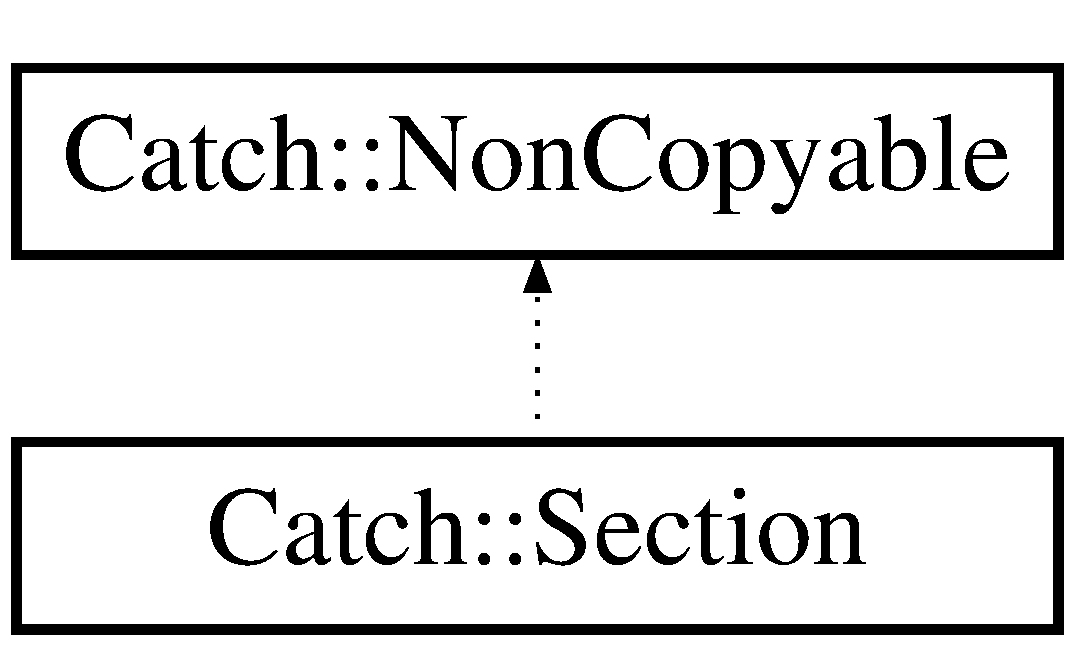
\includegraphics[height=2.000000cm]{classCatch_1_1Section}
\end{center}
\end{figure}
\subsection*{Public Member Functions}
\begin{DoxyCompactItemize}
\item 
\hyperlink{classCatch_1_1Section_a68fd4e51e8981aaa7ddb00d8a6abd099}{Section} (\hyperlink{structCatch_1_1SectionInfo}{Section\-Info} const \&info)
\item 
\hyperlink{classCatch_1_1Section_aa1422edd68a77aa578b5cc6b8b69f86f}{$\sim$\-Section} ()
\item 
\hyperlink{classCatch_1_1Section_a6c9be48e8ba0611c4aa601102e706f3b}{operator bool} () const 
\end{DoxyCompactItemize}


\subsection{Constructor \& Destructor Documentation}
\hypertarget{classCatch_1_1Section_a68fd4e51e8981aaa7ddb00d8a6abd099}{\index{Catch\-::\-Section@{Catch\-::\-Section}!Section@{Section}}
\index{Section@{Section}!Catch::Section@{Catch\-::\-Section}}
\subsubsection[{Section}]{\setlength{\rightskip}{0pt plus 5cm}Catch\-::\-Section\-::\-Section (
\begin{DoxyParamCaption}
\item[{{\bf Section\-Info} const \&}]{info}
\end{DoxyParamCaption}
)}}\label{classCatch_1_1Section_a68fd4e51e8981aaa7ddb00d8a6abd099}
\hypertarget{classCatch_1_1Section_aa1422edd68a77aa578b5cc6b8b69f86f}{\index{Catch\-::\-Section@{Catch\-::\-Section}!$\sim$\-Section@{$\sim$\-Section}}
\index{$\sim$\-Section@{$\sim$\-Section}!Catch::Section@{Catch\-::\-Section}}
\subsubsection[{$\sim$\-Section}]{\setlength{\rightskip}{0pt plus 5cm}Catch\-::\-Section\-::$\sim$\-Section (
\begin{DoxyParamCaption}
{}
\end{DoxyParamCaption}
)}}\label{classCatch_1_1Section_aa1422edd68a77aa578b5cc6b8b69f86f}


\subsection{Member Function Documentation}
\hypertarget{classCatch_1_1Section_a6c9be48e8ba0611c4aa601102e706f3b}{\index{Catch\-::\-Section@{Catch\-::\-Section}!operator bool@{operator bool}}
\index{operator bool@{operator bool}!Catch::Section@{Catch\-::\-Section}}
\subsubsection[{operator bool}]{\setlength{\rightskip}{0pt plus 5cm}Catch\-::\-Section\-::operator bool (
\begin{DoxyParamCaption}
{}
\end{DoxyParamCaption}
) const}}\label{classCatch_1_1Section_a6c9be48e8ba0611c4aa601102e706f3b}


The documentation for this class was generated from the following file\-:\begin{DoxyCompactItemize}
\item 
/home/alexander/\-Un\-B/\-M\-P/\-Trabalho\-\_\-2\-\_\-\-M\-P\-\_\-\-Alexander\-\_\-13\-\_\-0039853/include/\hyperlink{catch_8hpp}{catch.\-hpp}\end{DoxyCompactItemize}

\hypertarget{structCatch_1_1SectionEndInfo}{\section{Catch\-:\-:Section\-End\-Info Struct Reference}
\label{structCatch_1_1SectionEndInfo}\index{Catch\-::\-Section\-End\-Info@{Catch\-::\-Section\-End\-Info}}
}


{\ttfamily \#include $<$catch.\-hpp$>$}

\subsection*{Public Member Functions}
\begin{DoxyCompactItemize}
\item 
\hyperlink{structCatch_1_1SectionEndInfo_abc9381c7c22b6907317ec985ccaa6713}{Section\-End\-Info} (\hyperlink{structCatch_1_1SectionInfo}{Section\-Info} const \&\-\_\-section\-Info, \hyperlink{structCatch_1_1Counts}{Counts} const \&\-\_\-prev\-Assertions, double \-\_\-duration\-In\-Seconds)
\end{DoxyCompactItemize}
\subsection*{Public Attributes}
\begin{DoxyCompactItemize}
\item 
\hyperlink{structCatch_1_1SectionInfo}{Section\-Info} \hyperlink{structCatch_1_1SectionEndInfo_a2d44793392cb83735d086d726822abe9}{section\-Info}
\item 
\hyperlink{structCatch_1_1Counts}{Counts} \hyperlink{structCatch_1_1SectionEndInfo_ae70b154cbc05b5dd2901d97f89303d8c}{prev\-Assertions}
\item 
double \hyperlink{structCatch_1_1SectionEndInfo_a7c262f2dab9cff166b8eca620c47eea5}{duration\-In\-Seconds}
\end{DoxyCompactItemize}


\subsection{Constructor \& Destructor Documentation}
\hypertarget{structCatch_1_1SectionEndInfo_abc9381c7c22b6907317ec985ccaa6713}{\index{Catch\-::\-Section\-End\-Info@{Catch\-::\-Section\-End\-Info}!Section\-End\-Info@{Section\-End\-Info}}
\index{Section\-End\-Info@{Section\-End\-Info}!Catch::SectionEndInfo@{Catch\-::\-Section\-End\-Info}}
\subsubsection[{Section\-End\-Info}]{\setlength{\rightskip}{0pt plus 5cm}Catch\-::\-Section\-End\-Info\-::\-Section\-End\-Info (
\begin{DoxyParamCaption}
\item[{{\bf Section\-Info} const \&}]{\-\_\-section\-Info, }
\item[{{\bf Counts} const \&}]{\-\_\-prev\-Assertions, }
\item[{double}]{\-\_\-duration\-In\-Seconds}
\end{DoxyParamCaption}
)\hspace{0.3cm}{\ttfamily [inline]}}}\label{structCatch_1_1SectionEndInfo_abc9381c7c22b6907317ec985ccaa6713}


\subsection{Member Data Documentation}
\hypertarget{structCatch_1_1SectionEndInfo_a7c262f2dab9cff166b8eca620c47eea5}{\index{Catch\-::\-Section\-End\-Info@{Catch\-::\-Section\-End\-Info}!duration\-In\-Seconds@{duration\-In\-Seconds}}
\index{duration\-In\-Seconds@{duration\-In\-Seconds}!Catch::SectionEndInfo@{Catch\-::\-Section\-End\-Info}}
\subsubsection[{duration\-In\-Seconds}]{\setlength{\rightskip}{0pt plus 5cm}double Catch\-::\-Section\-End\-Info\-::duration\-In\-Seconds}}\label{structCatch_1_1SectionEndInfo_a7c262f2dab9cff166b8eca620c47eea5}
\hypertarget{structCatch_1_1SectionEndInfo_ae70b154cbc05b5dd2901d97f89303d8c}{\index{Catch\-::\-Section\-End\-Info@{Catch\-::\-Section\-End\-Info}!prev\-Assertions@{prev\-Assertions}}
\index{prev\-Assertions@{prev\-Assertions}!Catch::SectionEndInfo@{Catch\-::\-Section\-End\-Info}}
\subsubsection[{prev\-Assertions}]{\setlength{\rightskip}{0pt plus 5cm}{\bf Counts} Catch\-::\-Section\-End\-Info\-::prev\-Assertions}}\label{structCatch_1_1SectionEndInfo_ae70b154cbc05b5dd2901d97f89303d8c}
\hypertarget{structCatch_1_1SectionEndInfo_a2d44793392cb83735d086d726822abe9}{\index{Catch\-::\-Section\-End\-Info@{Catch\-::\-Section\-End\-Info}!section\-Info@{section\-Info}}
\index{section\-Info@{section\-Info}!Catch::SectionEndInfo@{Catch\-::\-Section\-End\-Info}}
\subsubsection[{section\-Info}]{\setlength{\rightskip}{0pt plus 5cm}{\bf Section\-Info} Catch\-::\-Section\-End\-Info\-::section\-Info}}\label{structCatch_1_1SectionEndInfo_a2d44793392cb83735d086d726822abe9}


The documentation for this struct was generated from the following file\-:\begin{DoxyCompactItemize}
\item 
/home/alexander/\-Un\-B/\-M\-P/\-Trabalho\-\_\-2\-\_\-\-M\-P\-\_\-\-Alexander\-\_\-13\-\_\-0039853/include/\hyperlink{catch_8hpp}{catch.\-hpp}\end{DoxyCompactItemize}

\hypertarget{structCatch_1_1SectionInfo}{\section{Catch\-:\-:Section\-Info Struct Reference}
\label{structCatch_1_1SectionInfo}\index{Catch\-::\-Section\-Info@{Catch\-::\-Section\-Info}}
}


{\ttfamily \#include $<$catch.\-hpp$>$}

\subsection*{Public Member Functions}
\begin{DoxyCompactItemize}
\item 
\hyperlink{structCatch_1_1SectionInfo_a27aff3aaf8b6611f3651b17111a272c6}{Section\-Info} (\hyperlink{structCatch_1_1SourceLineInfo}{Source\-Line\-Info} const \&\-\_\-line\-Info, std\-::string const \&\-\_\-name, std\-::string const \&\-\_\-description=std\-::string())
\end{DoxyCompactItemize}
\subsection*{Public Attributes}
\begin{DoxyCompactItemize}
\item 
std\-::string \hyperlink{structCatch_1_1SectionInfo_a704c8fc662d309137e0d4f199cb7df58}{name}
\item 
std\-::string \hyperlink{structCatch_1_1SectionInfo_a0052060219a6de74bb7ade34d4163a4e}{description}
\item 
\hyperlink{structCatch_1_1SourceLineInfo}{Source\-Line\-Info} \hyperlink{structCatch_1_1SectionInfo_adbc83b8a3507c4acc8ee249e93465711}{line\-Info}
\end{DoxyCompactItemize}


\subsection{Constructor \& Destructor Documentation}
\hypertarget{structCatch_1_1SectionInfo_a27aff3aaf8b6611f3651b17111a272c6}{\index{Catch\-::\-Section\-Info@{Catch\-::\-Section\-Info}!Section\-Info@{Section\-Info}}
\index{Section\-Info@{Section\-Info}!Catch::SectionInfo@{Catch\-::\-Section\-Info}}
\subsubsection[{Section\-Info}]{\setlength{\rightskip}{0pt plus 5cm}Catch\-::\-Section\-Info\-::\-Section\-Info (
\begin{DoxyParamCaption}
\item[{{\bf Source\-Line\-Info} const \&}]{\-\_\-line\-Info, }
\item[{std\-::string const \&}]{\-\_\-name, }
\item[{std\-::string const \&}]{\-\_\-description = {\ttfamily std\-:\-:string()}}
\end{DoxyParamCaption}
)}}\label{structCatch_1_1SectionInfo_a27aff3aaf8b6611f3651b17111a272c6}


\subsection{Member Data Documentation}
\hypertarget{structCatch_1_1SectionInfo_a0052060219a6de74bb7ade34d4163a4e}{\index{Catch\-::\-Section\-Info@{Catch\-::\-Section\-Info}!description@{description}}
\index{description@{description}!Catch::SectionInfo@{Catch\-::\-Section\-Info}}
\subsubsection[{description}]{\setlength{\rightskip}{0pt plus 5cm}std\-::string Catch\-::\-Section\-Info\-::description}}\label{structCatch_1_1SectionInfo_a0052060219a6de74bb7ade34d4163a4e}
\hypertarget{structCatch_1_1SectionInfo_adbc83b8a3507c4acc8ee249e93465711}{\index{Catch\-::\-Section\-Info@{Catch\-::\-Section\-Info}!line\-Info@{line\-Info}}
\index{line\-Info@{line\-Info}!Catch::SectionInfo@{Catch\-::\-Section\-Info}}
\subsubsection[{line\-Info}]{\setlength{\rightskip}{0pt plus 5cm}{\bf Source\-Line\-Info} Catch\-::\-Section\-Info\-::line\-Info}}\label{structCatch_1_1SectionInfo_adbc83b8a3507c4acc8ee249e93465711}
\hypertarget{structCatch_1_1SectionInfo_a704c8fc662d309137e0d4f199cb7df58}{\index{Catch\-::\-Section\-Info@{Catch\-::\-Section\-Info}!name@{name}}
\index{name@{name}!Catch::SectionInfo@{Catch\-::\-Section\-Info}}
\subsubsection[{name}]{\setlength{\rightskip}{0pt plus 5cm}std\-::string Catch\-::\-Section\-Info\-::name}}\label{structCatch_1_1SectionInfo_a704c8fc662d309137e0d4f199cb7df58}


The documentation for this struct was generated from the following file\-:\begin{DoxyCompactItemize}
\item 
/home/alexander/\-Un\-B/\-M\-P/\-Trabalho\-\_\-2\-\_\-\-M\-P\-\_\-\-Alexander\-\_\-13\-\_\-0039853/include/\hyperlink{catch_8hpp}{catch.\-hpp}\end{DoxyCompactItemize}

\hypertarget{structCatch_1_1SharedImpl}{\section{Catch\-:\-:Shared\-Impl$<$ T $>$ Struct Template Reference}
\label{structCatch_1_1SharedImpl}\index{Catch\-::\-Shared\-Impl$<$ T $>$@{Catch\-::\-Shared\-Impl$<$ T $>$}}
}


{\ttfamily \#include $<$catch.\-hpp$>$}

Inheritance diagram for Catch\-:\-:Shared\-Impl$<$ T $>$\-:\begin{figure}[H]
\begin{center}
\leavevmode
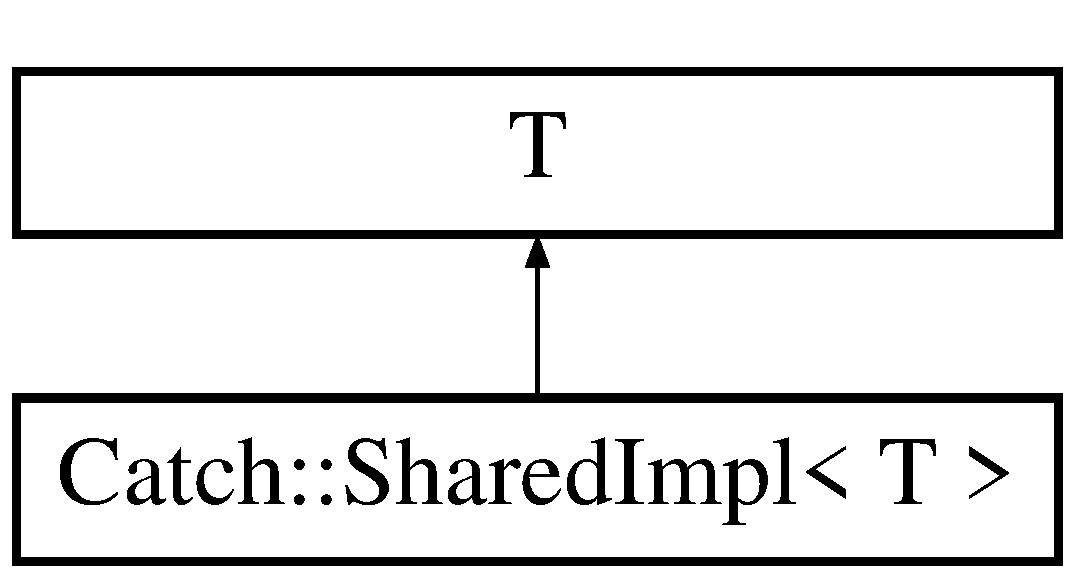
\includegraphics[height=2.000000cm]{structCatch_1_1SharedImpl}
\end{center}
\end{figure}
\subsection*{Public Member Functions}
\begin{DoxyCompactItemize}
\item 
\hyperlink{structCatch_1_1SharedImpl_a0629856ee353298b61ad52cf60e716fb}{Shared\-Impl} ()
\item 
virtual void \hyperlink{structCatch_1_1SharedImpl_a9b190b7a139a09d2624d1201d8e4f87e}{add\-Ref} () const 
\item 
virtual void \hyperlink{structCatch_1_1SharedImpl_a16baad80ad5ad3dfaf2a10a157a02e01}{release} () const 
\end{DoxyCompactItemize}
\subsection*{Public Attributes}
\begin{DoxyCompactItemize}
\item 
unsigned int \hyperlink{structCatch_1_1SharedImpl_a7e71ef1985b85aa41a1632f932a96bcb}{m\-\_\-rc}
\end{DoxyCompactItemize}


\subsection{Constructor \& Destructor Documentation}
\hypertarget{structCatch_1_1SharedImpl_a0629856ee353298b61ad52cf60e716fb}{\index{Catch\-::\-Shared\-Impl@{Catch\-::\-Shared\-Impl}!Shared\-Impl@{Shared\-Impl}}
\index{Shared\-Impl@{Shared\-Impl}!Catch::SharedImpl@{Catch\-::\-Shared\-Impl}}
\subsubsection[{Shared\-Impl}]{\setlength{\rightskip}{0pt plus 5cm}template$<$typename T = I\-Shared$>$ {\bf Catch\-::\-Shared\-Impl}$<$ T $>$\-::{\bf Shared\-Impl} (
\begin{DoxyParamCaption}
{}
\end{DoxyParamCaption}
)\hspace{0.3cm}{\ttfamily [inline]}}}\label{structCatch_1_1SharedImpl_a0629856ee353298b61ad52cf60e716fb}


\subsection{Member Function Documentation}
\hypertarget{structCatch_1_1SharedImpl_a9b190b7a139a09d2624d1201d8e4f87e}{\index{Catch\-::\-Shared\-Impl@{Catch\-::\-Shared\-Impl}!add\-Ref@{add\-Ref}}
\index{add\-Ref@{add\-Ref}!Catch::SharedImpl@{Catch\-::\-Shared\-Impl}}
\subsubsection[{add\-Ref}]{\setlength{\rightskip}{0pt plus 5cm}template$<$typename T = I\-Shared$>$ virtual void {\bf Catch\-::\-Shared\-Impl}$<$ T $>$\-::add\-Ref (
\begin{DoxyParamCaption}
{}
\end{DoxyParamCaption}
) const\hspace{0.3cm}{\ttfamily [inline]}, {\ttfamily [virtual]}}}\label{structCatch_1_1SharedImpl_a9b190b7a139a09d2624d1201d8e4f87e}
\hypertarget{structCatch_1_1SharedImpl_a16baad80ad5ad3dfaf2a10a157a02e01}{\index{Catch\-::\-Shared\-Impl@{Catch\-::\-Shared\-Impl}!release@{release}}
\index{release@{release}!Catch::SharedImpl@{Catch\-::\-Shared\-Impl}}
\subsubsection[{release}]{\setlength{\rightskip}{0pt plus 5cm}template$<$typename T = I\-Shared$>$ virtual void {\bf Catch\-::\-Shared\-Impl}$<$ T $>$\-::release (
\begin{DoxyParamCaption}
{}
\end{DoxyParamCaption}
) const\hspace{0.3cm}{\ttfamily [inline]}, {\ttfamily [virtual]}}}\label{structCatch_1_1SharedImpl_a16baad80ad5ad3dfaf2a10a157a02e01}


\subsection{Member Data Documentation}
\hypertarget{structCatch_1_1SharedImpl_a7e71ef1985b85aa41a1632f932a96bcb}{\index{Catch\-::\-Shared\-Impl@{Catch\-::\-Shared\-Impl}!m\-\_\-rc@{m\-\_\-rc}}
\index{m\-\_\-rc@{m\-\_\-rc}!Catch::SharedImpl@{Catch\-::\-Shared\-Impl}}
\subsubsection[{m\-\_\-rc}]{\setlength{\rightskip}{0pt plus 5cm}template$<$typename T = I\-Shared$>$ unsigned int {\bf Catch\-::\-Shared\-Impl}$<$ T $>$\-::m\-\_\-rc\hspace{0.3cm}{\ttfamily [mutable]}}}\label{structCatch_1_1SharedImpl_a7e71ef1985b85aa41a1632f932a96bcb}


The documentation for this struct was generated from the following file\-:\begin{DoxyCompactItemize}
\item 
/home/alexander/\-Un\-B/\-M\-P/\-Trabalho\-\_\-2\-\_\-\-M\-P\-\_\-\-Alexander\-\_\-13\-\_\-0039853/include/\hyperlink{catch_8hpp}{catch.\-hpp}\end{DoxyCompactItemize}

\hypertarget{structCatch_1_1SourceLineInfo}{\section{Catch\-:\-:Source\-Line\-Info Struct Reference}
\label{structCatch_1_1SourceLineInfo}\index{Catch\-::\-Source\-Line\-Info@{Catch\-::\-Source\-Line\-Info}}
}


{\ttfamily \#include $<$catch.\-hpp$>$}

\subsection*{Public Member Functions}
\begin{DoxyCompactItemize}
\item 
\hyperlink{structCatch_1_1SourceLineInfo_a9d44b2e1133794eee0bd5716424c83d6}{Source\-Line\-Info} ()
\item 
\hyperlink{structCatch_1_1SourceLineInfo_a6218cb890337d37f708ea94063958940}{Source\-Line\-Info} (char const $\ast$\-\_\-file, std\-::size\-\_\-t \-\_\-line)
\item 
bool \hyperlink{structCatch_1_1SourceLineInfo_a9a25ffc0640d1a3dd0c9b7e5fcbba7b9}{empty} () const 
\item 
bool \hyperlink{structCatch_1_1SourceLineInfo_af0854821b1abfda52796ef0f1294b050}{operator==} (\hyperlink{structCatch_1_1SourceLineInfo}{Source\-Line\-Info} const \&other) const 
\item 
bool \hyperlink{structCatch_1_1SourceLineInfo_a581c02d683808232168bfc2e775c3554}{operator$<$} (\hyperlink{structCatch_1_1SourceLineInfo}{Source\-Line\-Info} const \&other) const 
\end{DoxyCompactItemize}
\subsection*{Public Attributes}
\begin{DoxyCompactItemize}
\item 
char const $\ast$ \hyperlink{structCatch_1_1SourceLineInfo_ad65537703e9f08c1fa7777fbc3f0c617}{file}
\item 
std\-::size\-\_\-t \hyperlink{structCatch_1_1SourceLineInfo_a841e5d696c7b9cde24e45e61dd979c77}{line}
\end{DoxyCompactItemize}


\subsection{Constructor \& Destructor Documentation}
\hypertarget{structCatch_1_1SourceLineInfo_a9d44b2e1133794eee0bd5716424c83d6}{\index{Catch\-::\-Source\-Line\-Info@{Catch\-::\-Source\-Line\-Info}!Source\-Line\-Info@{Source\-Line\-Info}}
\index{Source\-Line\-Info@{Source\-Line\-Info}!Catch::SourceLineInfo@{Catch\-::\-Source\-Line\-Info}}
\subsubsection[{Source\-Line\-Info}]{\setlength{\rightskip}{0pt plus 5cm}Catch\-::\-Source\-Line\-Info\-::\-Source\-Line\-Info (
\begin{DoxyParamCaption}
{}
\end{DoxyParamCaption}
)}}\label{structCatch_1_1SourceLineInfo_a9d44b2e1133794eee0bd5716424c83d6}
\hypertarget{structCatch_1_1SourceLineInfo_a6218cb890337d37f708ea94063958940}{\index{Catch\-::\-Source\-Line\-Info@{Catch\-::\-Source\-Line\-Info}!Source\-Line\-Info@{Source\-Line\-Info}}
\index{Source\-Line\-Info@{Source\-Line\-Info}!Catch::SourceLineInfo@{Catch\-::\-Source\-Line\-Info}}
\subsubsection[{Source\-Line\-Info}]{\setlength{\rightskip}{0pt plus 5cm}Catch\-::\-Source\-Line\-Info\-::\-Source\-Line\-Info (
\begin{DoxyParamCaption}
\item[{char const $\ast$}]{\-\_\-file, }
\item[{std\-::size\-\_\-t}]{\-\_\-line}
\end{DoxyParamCaption}
)}}\label{structCatch_1_1SourceLineInfo_a6218cb890337d37f708ea94063958940}


\subsection{Member Function Documentation}
\hypertarget{structCatch_1_1SourceLineInfo_a9a25ffc0640d1a3dd0c9b7e5fcbba7b9}{\index{Catch\-::\-Source\-Line\-Info@{Catch\-::\-Source\-Line\-Info}!empty@{empty}}
\index{empty@{empty}!Catch::SourceLineInfo@{Catch\-::\-Source\-Line\-Info}}
\subsubsection[{empty}]{\setlength{\rightskip}{0pt plus 5cm}bool Catch\-::\-Source\-Line\-Info\-::empty (
\begin{DoxyParamCaption}
{}
\end{DoxyParamCaption}
) const}}\label{structCatch_1_1SourceLineInfo_a9a25ffc0640d1a3dd0c9b7e5fcbba7b9}
\hypertarget{structCatch_1_1SourceLineInfo_a581c02d683808232168bfc2e775c3554}{\index{Catch\-::\-Source\-Line\-Info@{Catch\-::\-Source\-Line\-Info}!operator$<$@{operator$<$}}
\index{operator$<$@{operator$<$}!Catch::SourceLineInfo@{Catch\-::\-Source\-Line\-Info}}
\subsubsection[{operator$<$}]{\setlength{\rightskip}{0pt plus 5cm}bool Catch\-::\-Source\-Line\-Info\-::operator$<$ (
\begin{DoxyParamCaption}
\item[{{\bf Source\-Line\-Info} const \&}]{other}
\end{DoxyParamCaption}
) const}}\label{structCatch_1_1SourceLineInfo_a581c02d683808232168bfc2e775c3554}
\hypertarget{structCatch_1_1SourceLineInfo_af0854821b1abfda52796ef0f1294b050}{\index{Catch\-::\-Source\-Line\-Info@{Catch\-::\-Source\-Line\-Info}!operator==@{operator==}}
\index{operator==@{operator==}!Catch::SourceLineInfo@{Catch\-::\-Source\-Line\-Info}}
\subsubsection[{operator==}]{\setlength{\rightskip}{0pt plus 5cm}bool Catch\-::\-Source\-Line\-Info\-::operator== (
\begin{DoxyParamCaption}
\item[{{\bf Source\-Line\-Info} const \&}]{other}
\end{DoxyParamCaption}
) const}}\label{structCatch_1_1SourceLineInfo_af0854821b1abfda52796ef0f1294b050}


\subsection{Member Data Documentation}
\hypertarget{structCatch_1_1SourceLineInfo_ad65537703e9f08c1fa7777fbc3f0c617}{\index{Catch\-::\-Source\-Line\-Info@{Catch\-::\-Source\-Line\-Info}!file@{file}}
\index{file@{file}!Catch::SourceLineInfo@{Catch\-::\-Source\-Line\-Info}}
\subsubsection[{file}]{\setlength{\rightskip}{0pt plus 5cm}char const$\ast$ Catch\-::\-Source\-Line\-Info\-::file}}\label{structCatch_1_1SourceLineInfo_ad65537703e9f08c1fa7777fbc3f0c617}
\hypertarget{structCatch_1_1SourceLineInfo_a841e5d696c7b9cde24e45e61dd979c77}{\index{Catch\-::\-Source\-Line\-Info@{Catch\-::\-Source\-Line\-Info}!line@{line}}
\index{line@{line}!Catch::SourceLineInfo@{Catch\-::\-Source\-Line\-Info}}
\subsubsection[{line}]{\setlength{\rightskip}{0pt plus 5cm}std\-::size\-\_\-t Catch\-::\-Source\-Line\-Info\-::line}}\label{structCatch_1_1SourceLineInfo_a841e5d696c7b9cde24e45e61dd979c77}


The documentation for this struct was generated from the following file\-:\begin{DoxyCompactItemize}
\item 
/home/alexander/\-Un\-B/\-M\-P/\-Trabalho\-\_\-2\-\_\-\-M\-P\-\_\-\-Alexander\-\_\-13\-\_\-0039853/include/\hyperlink{catch_8hpp}{catch.\-hpp}\end{DoxyCompactItemize}

\hypertarget{structCatch_1_1Matchers_1_1StdString_1_1StartsWithMatcher}{\section{Catch\-:\-:Matchers\-:\-:Std\-String\-:\-:Starts\-With\-Matcher Struct Reference}
\label{structCatch_1_1Matchers_1_1StdString_1_1StartsWithMatcher}\index{Catch\-::\-Matchers\-::\-Std\-String\-::\-Starts\-With\-Matcher@{Catch\-::\-Matchers\-::\-Std\-String\-::\-Starts\-With\-Matcher}}
}


{\ttfamily \#include $<$catch.\-hpp$>$}

Inheritance diagram for Catch\-:\-:Matchers\-:\-:Std\-String\-:\-:Starts\-With\-Matcher\-:\begin{figure}[H]
\begin{center}
\leavevmode
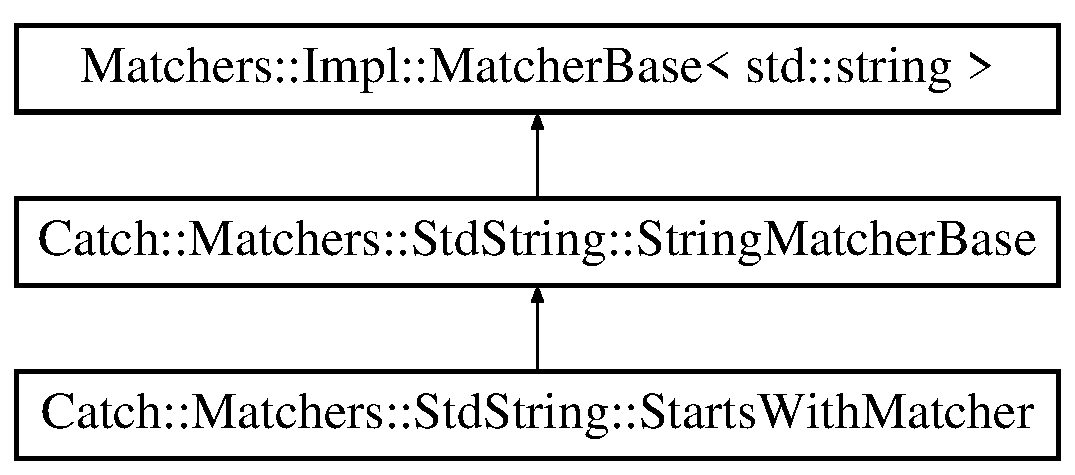
\includegraphics[height=3.000000cm]{structCatch_1_1Matchers_1_1StdString_1_1StartsWithMatcher}
\end{center}
\end{figure}
\subsection*{Public Member Functions}
\begin{DoxyCompactItemize}
\item 
\hyperlink{structCatch_1_1Matchers_1_1StdString_1_1StartsWithMatcher_a7b86f258bdbd131a6e7bcd94a8977325}{Starts\-With\-Matcher} (\hyperlink{structCatch_1_1Matchers_1_1StdString_1_1CasedString}{Cased\-String} const \&comparator)
\item 
virtual bool \hyperlink{structCatch_1_1Matchers_1_1StdString_1_1StartsWithMatcher_a0d37b1ddba7f1031e360ccd475f05d0d}{match} (std\-::string const \&source) const \hyperlink{catch_8hpp_a8ecdce4d3f57835f707915ae831eb847}{C\-A\-T\-C\-H\-\_\-\-O\-V\-E\-R\-R\-I\-D\-E}
\end{DoxyCompactItemize}
\subsection*{Additional Inherited Members}


\subsection{Constructor \& Destructor Documentation}
\hypertarget{structCatch_1_1Matchers_1_1StdString_1_1StartsWithMatcher_a7b86f258bdbd131a6e7bcd94a8977325}{\index{Catch\-::\-Matchers\-::\-Std\-String\-::\-Starts\-With\-Matcher@{Catch\-::\-Matchers\-::\-Std\-String\-::\-Starts\-With\-Matcher}!Starts\-With\-Matcher@{Starts\-With\-Matcher}}
\index{Starts\-With\-Matcher@{Starts\-With\-Matcher}!Catch::Matchers::StdString::StartsWithMatcher@{Catch\-::\-Matchers\-::\-Std\-String\-::\-Starts\-With\-Matcher}}
\subsubsection[{Starts\-With\-Matcher}]{\setlength{\rightskip}{0pt plus 5cm}Catch\-::\-Matchers\-::\-Std\-String\-::\-Starts\-With\-Matcher\-::\-Starts\-With\-Matcher (
\begin{DoxyParamCaption}
\item[{{\bf Cased\-String} const \&}]{comparator}
\end{DoxyParamCaption}
)}}\label{structCatch_1_1Matchers_1_1StdString_1_1StartsWithMatcher_a7b86f258bdbd131a6e7bcd94a8977325}


\subsection{Member Function Documentation}
\hypertarget{structCatch_1_1Matchers_1_1StdString_1_1StartsWithMatcher_a0d37b1ddba7f1031e360ccd475f05d0d}{\index{Catch\-::\-Matchers\-::\-Std\-String\-::\-Starts\-With\-Matcher@{Catch\-::\-Matchers\-::\-Std\-String\-::\-Starts\-With\-Matcher}!match@{match}}
\index{match@{match}!Catch::Matchers::StdString::StartsWithMatcher@{Catch\-::\-Matchers\-::\-Std\-String\-::\-Starts\-With\-Matcher}}
\subsubsection[{match}]{\setlength{\rightskip}{0pt plus 5cm}virtual bool Catch\-::\-Matchers\-::\-Std\-String\-::\-Starts\-With\-Matcher\-::match (
\begin{DoxyParamCaption}
\item[{std\-::string const \&}]{source}
\end{DoxyParamCaption}
) const\hspace{0.3cm}{\ttfamily [virtual]}}}\label{structCatch_1_1Matchers_1_1StdString_1_1StartsWithMatcher_a0d37b1ddba7f1031e360ccd475f05d0d}


The documentation for this struct was generated from the following file\-:\begin{DoxyCompactItemize}
\item 
/home/alexander/\-Un\-B/\-M\-P/\-Trabalho\-\_\-2\-\_\-\-M\-P\-\_\-\-Alexander\-\_\-13\-\_\-0039853/include/\hyperlink{catch_8hpp}{catch.\-hpp}\end{DoxyCompactItemize}

\hypertarget{structCatch_1_1StreamEndStop}{\section{Catch\-:\-:Stream\-End\-Stop Struct Reference}
\label{structCatch_1_1StreamEndStop}\index{Catch\-::\-Stream\-End\-Stop@{Catch\-::\-Stream\-End\-Stop}}
}


{\ttfamily \#include $<$catch.\-hpp$>$}

\subsection*{Public Member Functions}
\begin{DoxyCompactItemize}
\item 
std\-::string \hyperlink{structCatch_1_1StreamEndStop_a3025092e06c224e0845f2caa07b26d0e}{operator+} ()
\end{DoxyCompactItemize}


\subsection{Member Function Documentation}
\hypertarget{structCatch_1_1StreamEndStop_a3025092e06c224e0845f2caa07b26d0e}{\index{Catch\-::\-Stream\-End\-Stop@{Catch\-::\-Stream\-End\-Stop}!operator+@{operator+}}
\index{operator+@{operator+}!Catch::StreamEndStop@{Catch\-::\-Stream\-End\-Stop}}
\subsubsection[{operator+}]{\setlength{\rightskip}{0pt plus 5cm}std\-::string Catch\-::\-Stream\-End\-Stop\-::operator+ (
\begin{DoxyParamCaption}
{}
\end{DoxyParamCaption}
)\hspace{0.3cm}{\ttfamily [inline]}}}\label{structCatch_1_1StreamEndStop_a3025092e06c224e0845f2caa07b26d0e}


The documentation for this struct was generated from the following file\-:\begin{DoxyCompactItemize}
\item 
/home/alexander/\-Un\-B/\-M\-P/\-Trabalho\-\_\-2\-\_\-\-M\-P\-\_\-\-Alexander\-\_\-13\-\_\-0039853/include/\hyperlink{catch_8hpp}{catch.\-hpp}\end{DoxyCompactItemize}

\hypertarget{structCatch_1_1StringMaker}{\section{Catch\-:\-:String\-Maker$<$ T $>$ Struct Template Reference}
\label{structCatch_1_1StringMaker}\index{Catch\-::\-String\-Maker$<$ T $>$@{Catch\-::\-String\-Maker$<$ T $>$}}
}


{\ttfamily \#include $<$catch.\-hpp$>$}

Inheritance diagram for Catch\-:\-:String\-Maker$<$ T $>$\-:\begin{figure}[H]
\begin{center}
\leavevmode
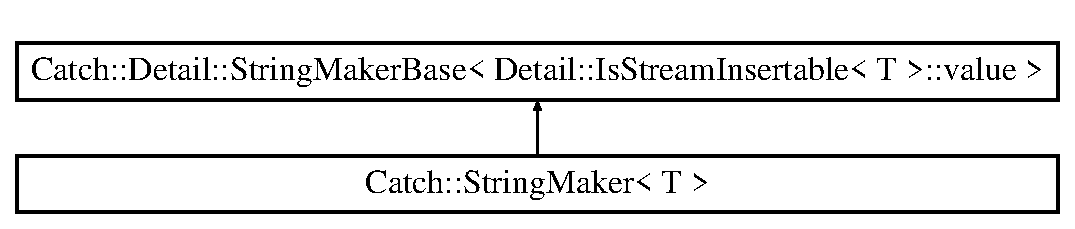
\includegraphics[height=2.000000cm]{structCatch_1_1StringMaker}
\end{center}
\end{figure}
\subsection*{Additional Inherited Members}


The documentation for this struct was generated from the following file\-:\begin{DoxyCompactItemize}
\item 
/home/alexander/\-Un\-B/\-M\-P/\-Trabalho\-\_\-2\-\_\-\-M\-P\-\_\-\-Alexander\-\_\-13\-\_\-0039853/include/\hyperlink{catch_8hpp}{catch.\-hpp}\end{DoxyCompactItemize}

\hypertarget{structCatch_1_1StringMaker_3_01R_01C_1_1_5_01_4}{\section{Catch\-:\-:String\-Maker$<$ R C\-:\-:$\ast$ $>$ Struct Template Reference}
\label{structCatch_1_1StringMaker_3_01R_01C_1_1_5_01_4}\index{Catch\-::\-String\-Maker$<$ R C\-::$\ast$ $>$@{Catch\-::\-String\-Maker$<$ R C\-::$\ast$ $>$}}
}


{\ttfamily \#include $<$catch.\-hpp$>$}

\subsection*{Static Public Member Functions}
\begin{DoxyCompactItemize}
\item 
static std\-::string \hyperlink{structCatch_1_1StringMaker_3_01R_01C_1_1_5_01_4_af69c15e0b406e945777137fe4a333731}{convert} (R C\-::$\ast$p)
\end{DoxyCompactItemize}


\subsection{Member Function Documentation}
\hypertarget{structCatch_1_1StringMaker_3_01R_01C_1_1_5_01_4_af69c15e0b406e945777137fe4a333731}{\index{Catch\-::\-String\-Maker$<$ R C\-::$\ast$ $>$@{Catch\-::\-String\-Maker$<$ R C\-::$\ast$ $>$}!convert@{convert}}
\index{convert@{convert}!Catch::StringMaker< R C::* >@{Catch\-::\-String\-Maker$<$ R C\-::$\ast$ $>$}}
\subsubsection[{convert}]{\setlength{\rightskip}{0pt plus 5cm}template$<$typename R , typename C $>$ static std\-::string {\bf Catch\-::\-String\-Maker}$<$ R C\-::$\ast$ $>$\-::convert (
\begin{DoxyParamCaption}
\item[{R C\-::$\ast$}]{p}
\end{DoxyParamCaption}
)\hspace{0.3cm}{\ttfamily [inline]}, {\ttfamily [static]}}}\label{structCatch_1_1StringMaker_3_01R_01C_1_1_5_01_4_af69c15e0b406e945777137fe4a333731}


The documentation for this struct was generated from the following file\-:\begin{DoxyCompactItemize}
\item 
/home/alexander/\-Un\-B/\-M\-P/\-Trabalho\-\_\-2\-\_\-\-M\-P\-\_\-\-Alexander\-\_\-13\-\_\-0039853/include/\hyperlink{catch_8hpp}{catch.\-hpp}\end{DoxyCompactItemize}

\hypertarget{structCatch_1_1StringMaker_3_01T_01_5_01_4}{\section{Catch\-:\-:String\-Maker$<$ T $\ast$ $>$ Struct Template Reference}
\label{structCatch_1_1StringMaker_3_01T_01_5_01_4}\index{Catch\-::\-String\-Maker$<$ T $\ast$ $>$@{Catch\-::\-String\-Maker$<$ T $\ast$ $>$}}
}


{\ttfamily \#include $<$catch.\-hpp$>$}

\subsection*{Static Public Member Functions}
\begin{DoxyCompactItemize}
\item 
{\footnotesize template$<$typename U $>$ }\\static std\-::string \hyperlink{structCatch_1_1StringMaker_3_01T_01_5_01_4_a2adbc75c99d71b8323f4052bcb0815c9}{convert} (U $\ast$p)
\end{DoxyCompactItemize}


\subsection{Member Function Documentation}
\hypertarget{structCatch_1_1StringMaker_3_01T_01_5_01_4_a2adbc75c99d71b8323f4052bcb0815c9}{\index{Catch\-::\-String\-Maker$<$ T $\ast$ $>$@{Catch\-::\-String\-Maker$<$ T $\ast$ $>$}!convert@{convert}}
\index{convert@{convert}!Catch::StringMaker< T * >@{Catch\-::\-String\-Maker$<$ T $\ast$ $>$}}
\subsubsection[{convert}]{\setlength{\rightskip}{0pt plus 5cm}template$<$typename T $>$ template$<$typename U $>$ static std\-::string {\bf Catch\-::\-String\-Maker}$<$ T $\ast$ $>$\-::convert (
\begin{DoxyParamCaption}
\item[{U $\ast$}]{p}
\end{DoxyParamCaption}
)\hspace{0.3cm}{\ttfamily [inline]}, {\ttfamily [static]}}}\label{structCatch_1_1StringMaker_3_01T_01_5_01_4_a2adbc75c99d71b8323f4052bcb0815c9}


The documentation for this struct was generated from the following file\-:\begin{DoxyCompactItemize}
\item 
/home/alexander/\-Un\-B/\-M\-P/\-Trabalho\-\_\-2\-\_\-\-M\-P\-\_\-\-Alexander\-\_\-13\-\_\-0039853/include/\hyperlink{catch_8hpp}{catch.\-hpp}\end{DoxyCompactItemize}

\hypertarget{structCatch_1_1Detail_1_1StringMakerBase}{\section{Catch\-:\-:Detail\-:\-:String\-Maker\-Base$<$ C $>$ Struct Template Reference}
\label{structCatch_1_1Detail_1_1StringMakerBase}\index{Catch\-::\-Detail\-::\-String\-Maker\-Base$<$ C $>$@{Catch\-::\-Detail\-::\-String\-Maker\-Base$<$ C $>$}}
}


{\ttfamily \#include $<$catch.\-hpp$>$}

\subsection*{Static Public Member Functions}
\begin{DoxyCompactItemize}
\item 
{\footnotesize template$<$typename T $>$ }\\static std\-::string \hyperlink{structCatch_1_1Detail_1_1StringMakerBase_a8eb9f635dc413a5758e22614bafaf1a3}{convert} (T const \&)
\end{DoxyCompactItemize}


\subsection{Member Function Documentation}
\hypertarget{structCatch_1_1Detail_1_1StringMakerBase_a8eb9f635dc413a5758e22614bafaf1a3}{\index{Catch\-::\-Detail\-::\-String\-Maker\-Base@{Catch\-::\-Detail\-::\-String\-Maker\-Base}!convert@{convert}}
\index{convert@{convert}!Catch::Detail::StringMakerBase@{Catch\-::\-Detail\-::\-String\-Maker\-Base}}
\subsubsection[{convert}]{\setlength{\rightskip}{0pt plus 5cm}template$<$bool C$>$ template$<$typename T $>$ static std\-::string {\bf Catch\-::\-Detail\-::\-String\-Maker\-Base}$<$ C $>$\-::convert (
\begin{DoxyParamCaption}
\item[{T const \&}]{}
\end{DoxyParamCaption}
)\hspace{0.3cm}{\ttfamily [inline]}, {\ttfamily [static]}}}\label{structCatch_1_1Detail_1_1StringMakerBase_a8eb9f635dc413a5758e22614bafaf1a3}


The documentation for this struct was generated from the following file\-:\begin{DoxyCompactItemize}
\item 
/home/alexander/\-Un\-B/\-M\-P/\-Trabalho\-\_\-2\-\_\-\-M\-P\-\_\-\-Alexander\-\_\-13\-\_\-0039853/include/\hyperlink{catch_8hpp}{catch.\-hpp}\end{DoxyCompactItemize}

\hypertarget{structCatch_1_1Detail_1_1StringMakerBase_3_01true_01_4}{\section{Catch\-:\-:Detail\-:\-:String\-Maker\-Base$<$ true $>$ Struct Template Reference}
\label{structCatch_1_1Detail_1_1StringMakerBase_3_01true_01_4}\index{Catch\-::\-Detail\-::\-String\-Maker\-Base$<$ true $>$@{Catch\-::\-Detail\-::\-String\-Maker\-Base$<$ true $>$}}
}


{\ttfamily \#include $<$catch.\-hpp$>$}

\subsection*{Static Public Member Functions}
\begin{DoxyCompactItemize}
\item 
{\footnotesize template$<$typename T $>$ }\\static std\-::string \hyperlink{structCatch_1_1Detail_1_1StringMakerBase_3_01true_01_4_af9b5fdf7fddd8c5c873caa819e5f00f6}{convert} (T const \&\-\_\-value)
\end{DoxyCompactItemize}


\subsection{Member Function Documentation}
\hypertarget{structCatch_1_1Detail_1_1StringMakerBase_3_01true_01_4_af9b5fdf7fddd8c5c873caa819e5f00f6}{\index{Catch\-::\-Detail\-::\-String\-Maker\-Base$<$ true $>$@{Catch\-::\-Detail\-::\-String\-Maker\-Base$<$ true $>$}!convert@{convert}}
\index{convert@{convert}!Catch::Detail::StringMakerBase< true >@{Catch\-::\-Detail\-::\-String\-Maker\-Base$<$ true $>$}}
\subsubsection[{convert}]{\setlength{\rightskip}{0pt plus 5cm}template$<$typename T $>$ static std\-::string {\bf Catch\-::\-Detail\-::\-String\-Maker\-Base}$<$ true $>$\-::convert (
\begin{DoxyParamCaption}
\item[{T const \&}]{\-\_\-value}
\end{DoxyParamCaption}
)\hspace{0.3cm}{\ttfamily [inline]}, {\ttfamily [static]}}}\label{structCatch_1_1Detail_1_1StringMakerBase_3_01true_01_4_af9b5fdf7fddd8c5c873caa819e5f00f6}


The documentation for this struct was generated from the following file\-:\begin{DoxyCompactItemize}
\item 
/home/alexander/\-Un\-B/\-M\-P/\-Trabalho\-\_\-2\-\_\-\-M\-P\-\_\-\-Alexander\-\_\-13\-\_\-0039853/include/\hyperlink{catch_8hpp}{catch.\-hpp}\end{DoxyCompactItemize}

\hypertarget{structCatch_1_1Matchers_1_1StdString_1_1StringMatcherBase}{\section{Catch\-:\-:Matchers\-:\-:Std\-String\-:\-:String\-Matcher\-Base Struct Reference}
\label{structCatch_1_1Matchers_1_1StdString_1_1StringMatcherBase}\index{Catch\-::\-Matchers\-::\-Std\-String\-::\-String\-Matcher\-Base@{Catch\-::\-Matchers\-::\-Std\-String\-::\-String\-Matcher\-Base}}
}


{\ttfamily \#include $<$catch.\-hpp$>$}

Inheritance diagram for Catch\-:\-:Matchers\-:\-:Std\-String\-:\-:String\-Matcher\-Base\-:\begin{figure}[H]
\begin{center}
\leavevmode
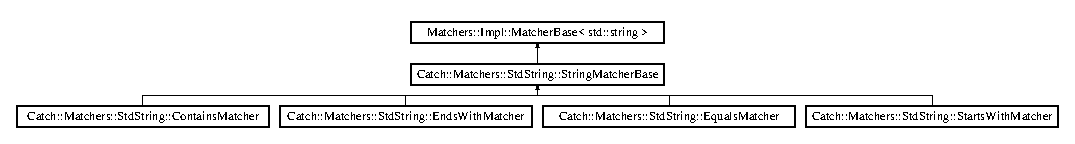
\includegraphics[height=1.484099cm]{structCatch_1_1Matchers_1_1StdString_1_1StringMatcherBase}
\end{center}
\end{figure}
\subsection*{Public Member Functions}
\begin{DoxyCompactItemize}
\item 
\hyperlink{structCatch_1_1Matchers_1_1StdString_1_1StringMatcherBase_a3a9b66bae298ae27058478529b4bb39d}{String\-Matcher\-Base} (std\-::string const \&operation, \hyperlink{structCatch_1_1Matchers_1_1StdString_1_1CasedString}{Cased\-String} const \&comparator)
\item 
virtual std\-::string \hyperlink{structCatch_1_1Matchers_1_1StdString_1_1StringMatcherBase_a9d15cfb882efbea778b2ed29e7f48f37}{describe} () const \hyperlink{catch_8hpp_a8ecdce4d3f57835f707915ae831eb847}{C\-A\-T\-C\-H\-\_\-\-O\-V\-E\-R\-R\-I\-D\-E}
\end{DoxyCompactItemize}
\subsection*{Public Attributes}
\begin{DoxyCompactItemize}
\item 
\hyperlink{structCatch_1_1Matchers_1_1StdString_1_1CasedString}{Cased\-String} \hyperlink{structCatch_1_1Matchers_1_1StdString_1_1StringMatcherBase_a17c9f0fe40587070ffe998c193742831}{m\-\_\-comparator}
\item 
std\-::string \hyperlink{structCatch_1_1Matchers_1_1StdString_1_1StringMatcherBase_a7a25c4b7d863e9a1c406d81efd0f83ca}{m\-\_\-operation}
\end{DoxyCompactItemize}


\subsection{Constructor \& Destructor Documentation}
\hypertarget{structCatch_1_1Matchers_1_1StdString_1_1StringMatcherBase_a3a9b66bae298ae27058478529b4bb39d}{\index{Catch\-::\-Matchers\-::\-Std\-String\-::\-String\-Matcher\-Base@{Catch\-::\-Matchers\-::\-Std\-String\-::\-String\-Matcher\-Base}!String\-Matcher\-Base@{String\-Matcher\-Base}}
\index{String\-Matcher\-Base@{String\-Matcher\-Base}!Catch::Matchers::StdString::StringMatcherBase@{Catch\-::\-Matchers\-::\-Std\-String\-::\-String\-Matcher\-Base}}
\subsubsection[{String\-Matcher\-Base}]{\setlength{\rightskip}{0pt plus 5cm}Catch\-::\-Matchers\-::\-Std\-String\-::\-String\-Matcher\-Base\-::\-String\-Matcher\-Base (
\begin{DoxyParamCaption}
\item[{std\-::string const \&}]{operation, }
\item[{{\bf Cased\-String} const \&}]{comparator}
\end{DoxyParamCaption}
)}}\label{structCatch_1_1Matchers_1_1StdString_1_1StringMatcherBase_a3a9b66bae298ae27058478529b4bb39d}


\subsection{Member Function Documentation}
\hypertarget{structCatch_1_1Matchers_1_1StdString_1_1StringMatcherBase_a9d15cfb882efbea778b2ed29e7f48f37}{\index{Catch\-::\-Matchers\-::\-Std\-String\-::\-String\-Matcher\-Base@{Catch\-::\-Matchers\-::\-Std\-String\-::\-String\-Matcher\-Base}!describe@{describe}}
\index{describe@{describe}!Catch::Matchers::StdString::StringMatcherBase@{Catch\-::\-Matchers\-::\-Std\-String\-::\-String\-Matcher\-Base}}
\subsubsection[{describe}]{\setlength{\rightskip}{0pt plus 5cm}virtual std\-::string Catch\-::\-Matchers\-::\-Std\-String\-::\-String\-Matcher\-Base\-::describe (
\begin{DoxyParamCaption}
{}
\end{DoxyParamCaption}
) const\hspace{0.3cm}{\ttfamily [virtual]}}}\label{structCatch_1_1Matchers_1_1StdString_1_1StringMatcherBase_a9d15cfb882efbea778b2ed29e7f48f37}


\subsection{Member Data Documentation}
\hypertarget{structCatch_1_1Matchers_1_1StdString_1_1StringMatcherBase_a17c9f0fe40587070ffe998c193742831}{\index{Catch\-::\-Matchers\-::\-Std\-String\-::\-String\-Matcher\-Base@{Catch\-::\-Matchers\-::\-Std\-String\-::\-String\-Matcher\-Base}!m\-\_\-comparator@{m\-\_\-comparator}}
\index{m\-\_\-comparator@{m\-\_\-comparator}!Catch::Matchers::StdString::StringMatcherBase@{Catch\-::\-Matchers\-::\-Std\-String\-::\-String\-Matcher\-Base}}
\subsubsection[{m\-\_\-comparator}]{\setlength{\rightskip}{0pt plus 5cm}{\bf Cased\-String} Catch\-::\-Matchers\-::\-Std\-String\-::\-String\-Matcher\-Base\-::m\-\_\-comparator}}\label{structCatch_1_1Matchers_1_1StdString_1_1StringMatcherBase_a17c9f0fe40587070ffe998c193742831}
\hypertarget{structCatch_1_1Matchers_1_1StdString_1_1StringMatcherBase_a7a25c4b7d863e9a1c406d81efd0f83ca}{\index{Catch\-::\-Matchers\-::\-Std\-String\-::\-String\-Matcher\-Base@{Catch\-::\-Matchers\-::\-Std\-String\-::\-String\-Matcher\-Base}!m\-\_\-operation@{m\-\_\-operation}}
\index{m\-\_\-operation@{m\-\_\-operation}!Catch::Matchers::StdString::StringMatcherBase@{Catch\-::\-Matchers\-::\-Std\-String\-::\-String\-Matcher\-Base}}
\subsubsection[{m\-\_\-operation}]{\setlength{\rightskip}{0pt plus 5cm}std\-::string Catch\-::\-Matchers\-::\-Std\-String\-::\-String\-Matcher\-Base\-::m\-\_\-operation}}\label{structCatch_1_1Matchers_1_1StdString_1_1StringMatcherBase_a7a25c4b7d863e9a1c406d81efd0f83ca}


The documentation for this struct was generated from the following file\-:\begin{DoxyCompactItemize}
\item 
/home/alexander/\-Un\-B/\-M\-P/\-Trabalho\-\_\-2\-\_\-\-M\-P\-\_\-\-Alexander\-\_\-13\-\_\-0039853/include/\hyperlink{catch_8hpp}{catch.\-hpp}\end{DoxyCompactItemize}

\hypertarget{structCatch_1_1TagAlias}{\section{Catch\-:\-:Tag\-Alias Struct Reference}
\label{structCatch_1_1TagAlias}\index{Catch\-::\-Tag\-Alias@{Catch\-::\-Tag\-Alias}}
}


{\ttfamily \#include $<$catch.\-hpp$>$}

\subsection*{Public Member Functions}
\begin{DoxyCompactItemize}
\item 
\hyperlink{structCatch_1_1TagAlias_ae5a030edfbc8e37f28310d4ca599396c}{Tag\-Alias} (std\-::string const \&\-\_\-tag, \hyperlink{structCatch_1_1SourceLineInfo}{Source\-Line\-Info} \-\_\-line\-Info)
\end{DoxyCompactItemize}
\subsection*{Public Attributes}
\begin{DoxyCompactItemize}
\item 
std\-::string \hyperlink{structCatch_1_1TagAlias_a950183883ab17c90d0fab16b966b6e2d}{tag}
\item 
\hyperlink{structCatch_1_1SourceLineInfo}{Source\-Line\-Info} \hyperlink{structCatch_1_1TagAlias_a2f51fe0b3c052561275d26b6eb88f702}{line\-Info}
\end{DoxyCompactItemize}


\subsection{Constructor \& Destructor Documentation}
\hypertarget{structCatch_1_1TagAlias_ae5a030edfbc8e37f28310d4ca599396c}{\index{Catch\-::\-Tag\-Alias@{Catch\-::\-Tag\-Alias}!Tag\-Alias@{Tag\-Alias}}
\index{Tag\-Alias@{Tag\-Alias}!Catch::TagAlias@{Catch\-::\-Tag\-Alias}}
\subsubsection[{Tag\-Alias}]{\setlength{\rightskip}{0pt plus 5cm}Catch\-::\-Tag\-Alias\-::\-Tag\-Alias (
\begin{DoxyParamCaption}
\item[{std\-::string const \&}]{\-\_\-tag, }
\item[{{\bf Source\-Line\-Info}}]{\-\_\-line\-Info}
\end{DoxyParamCaption}
)\hspace{0.3cm}{\ttfamily [inline]}}}\label{structCatch_1_1TagAlias_ae5a030edfbc8e37f28310d4ca599396c}


\subsection{Member Data Documentation}
\hypertarget{structCatch_1_1TagAlias_a2f51fe0b3c052561275d26b6eb88f702}{\index{Catch\-::\-Tag\-Alias@{Catch\-::\-Tag\-Alias}!line\-Info@{line\-Info}}
\index{line\-Info@{line\-Info}!Catch::TagAlias@{Catch\-::\-Tag\-Alias}}
\subsubsection[{line\-Info}]{\setlength{\rightskip}{0pt plus 5cm}{\bf Source\-Line\-Info} Catch\-::\-Tag\-Alias\-::line\-Info}}\label{structCatch_1_1TagAlias_a2f51fe0b3c052561275d26b6eb88f702}
\hypertarget{structCatch_1_1TagAlias_a950183883ab17c90d0fab16b966b6e2d}{\index{Catch\-::\-Tag\-Alias@{Catch\-::\-Tag\-Alias}!tag@{tag}}
\index{tag@{tag}!Catch::TagAlias@{Catch\-::\-Tag\-Alias}}
\subsubsection[{tag}]{\setlength{\rightskip}{0pt plus 5cm}std\-::string Catch\-::\-Tag\-Alias\-::tag}}\label{structCatch_1_1TagAlias_a950183883ab17c90d0fab16b966b6e2d}


The documentation for this struct was generated from the following file\-:\begin{DoxyCompactItemize}
\item 
/home/alexander/\-Un\-B/\-M\-P/\-Trabalho\-\_\-2\-\_\-\-M\-P\-\_\-\-Alexander\-\_\-13\-\_\-0039853/include/\hyperlink{catch_8hpp}{catch.\-hpp}\end{DoxyCompactItemize}

\hypertarget{classCatch_1_1TestCase}{\section{Catch\-:\-:Test\-Case Class Reference}
\label{classCatch_1_1TestCase}\index{Catch\-::\-Test\-Case@{Catch\-::\-Test\-Case}}
}


{\ttfamily \#include $<$catch.\-hpp$>$}

Inheritance diagram for Catch\-:\-:Test\-Case\-:\begin{figure}[H]
\begin{center}
\leavevmode
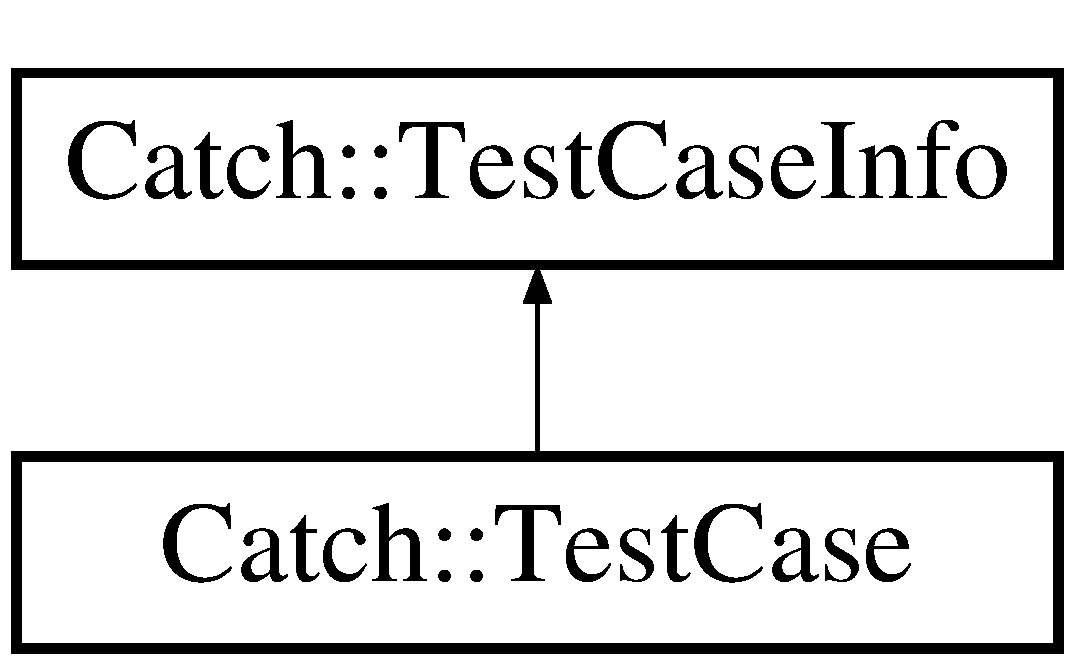
\includegraphics[height=2.000000cm]{classCatch_1_1TestCase}
\end{center}
\end{figure}
\subsection*{Public Member Functions}
\begin{DoxyCompactItemize}
\item 
\hyperlink{classCatch_1_1TestCase_a03a5b913484681bd6d398dc5e9c2a907}{Test\-Case} (\hyperlink{structCatch_1_1ITestCase}{I\-Test\-Case} $\ast$test\-Case, \hyperlink{structCatch_1_1TestCaseInfo}{Test\-Case\-Info} const \&info)
\item 
\hyperlink{classCatch_1_1TestCase_ac0011d3789edc3e44edb41f13c4775a0}{Test\-Case} (\hyperlink{classCatch_1_1TestCase}{Test\-Case} const \&other)
\item 
\hyperlink{classCatch_1_1TestCase}{Test\-Case} \hyperlink{classCatch_1_1TestCase_ab6dbc6c82b7c1680013c67bdedccfc8e}{with\-Name} (std\-::string const \&\-\_\-new\-Name) const 
\item 
void \hyperlink{classCatch_1_1TestCase_aac2e028135cc88c3e3aac04650960a6c}{invoke} () const 
\item 
\hyperlink{structCatch_1_1TestCaseInfo}{Test\-Case\-Info} const \& \hyperlink{classCatch_1_1TestCase_a25c03661ab092431cdff10df5c58a5a7}{get\-Test\-Case\-Info} () const 
\item 
void \hyperlink{classCatch_1_1TestCase_aee38f908faf10b905b209ca388275413}{swap} (\hyperlink{classCatch_1_1TestCase}{Test\-Case} \&other)
\item 
bool \hyperlink{classCatch_1_1TestCase_a40eab521b316c7d476f6b4dd1c33eec8}{operator==} (\hyperlink{classCatch_1_1TestCase}{Test\-Case} const \&other) const 
\item 
bool \hyperlink{classCatch_1_1TestCase_aa5174e85e3aac6e7398dee9c76730324}{operator$<$} (\hyperlink{classCatch_1_1TestCase}{Test\-Case} const \&other) const 
\item 
\hyperlink{classCatch_1_1TestCase}{Test\-Case} \& \hyperlink{classCatch_1_1TestCase_a8022e3f74232f7887d2d2cbbc8876502}{operator=} (\hyperlink{classCatch_1_1TestCase}{Test\-Case} const \&other)
\end{DoxyCompactItemize}
\subsection*{Additional Inherited Members}


\subsection{Constructor \& Destructor Documentation}
\hypertarget{classCatch_1_1TestCase_a03a5b913484681bd6d398dc5e9c2a907}{\index{Catch\-::\-Test\-Case@{Catch\-::\-Test\-Case}!Test\-Case@{Test\-Case}}
\index{Test\-Case@{Test\-Case}!Catch::TestCase@{Catch\-::\-Test\-Case}}
\subsubsection[{Test\-Case}]{\setlength{\rightskip}{0pt plus 5cm}Catch\-::\-Test\-Case\-::\-Test\-Case (
\begin{DoxyParamCaption}
\item[{{\bf I\-Test\-Case} $\ast$}]{test\-Case, }
\item[{{\bf Test\-Case\-Info} const \&}]{info}
\end{DoxyParamCaption}
)}}\label{classCatch_1_1TestCase_a03a5b913484681bd6d398dc5e9c2a907}
\hypertarget{classCatch_1_1TestCase_ac0011d3789edc3e44edb41f13c4775a0}{\index{Catch\-::\-Test\-Case@{Catch\-::\-Test\-Case}!Test\-Case@{Test\-Case}}
\index{Test\-Case@{Test\-Case}!Catch::TestCase@{Catch\-::\-Test\-Case}}
\subsubsection[{Test\-Case}]{\setlength{\rightskip}{0pt plus 5cm}Catch\-::\-Test\-Case\-::\-Test\-Case (
\begin{DoxyParamCaption}
\item[{{\bf Test\-Case} const \&}]{other}
\end{DoxyParamCaption}
)}}\label{classCatch_1_1TestCase_ac0011d3789edc3e44edb41f13c4775a0}


\subsection{Member Function Documentation}
\hypertarget{classCatch_1_1TestCase_a25c03661ab092431cdff10df5c58a5a7}{\index{Catch\-::\-Test\-Case@{Catch\-::\-Test\-Case}!get\-Test\-Case\-Info@{get\-Test\-Case\-Info}}
\index{get\-Test\-Case\-Info@{get\-Test\-Case\-Info}!Catch::TestCase@{Catch\-::\-Test\-Case}}
\subsubsection[{get\-Test\-Case\-Info}]{\setlength{\rightskip}{0pt plus 5cm}{\bf Test\-Case\-Info} const\& Catch\-::\-Test\-Case\-::get\-Test\-Case\-Info (
\begin{DoxyParamCaption}
{}
\end{DoxyParamCaption}
) const}}\label{classCatch_1_1TestCase_a25c03661ab092431cdff10df5c58a5a7}
\hypertarget{classCatch_1_1TestCase_aac2e028135cc88c3e3aac04650960a6c}{\index{Catch\-::\-Test\-Case@{Catch\-::\-Test\-Case}!invoke@{invoke}}
\index{invoke@{invoke}!Catch::TestCase@{Catch\-::\-Test\-Case}}
\subsubsection[{invoke}]{\setlength{\rightskip}{0pt plus 5cm}void Catch\-::\-Test\-Case\-::invoke (
\begin{DoxyParamCaption}
{}
\end{DoxyParamCaption}
) const}}\label{classCatch_1_1TestCase_aac2e028135cc88c3e3aac04650960a6c}
\hypertarget{classCatch_1_1TestCase_aa5174e85e3aac6e7398dee9c76730324}{\index{Catch\-::\-Test\-Case@{Catch\-::\-Test\-Case}!operator$<$@{operator$<$}}
\index{operator$<$@{operator$<$}!Catch::TestCase@{Catch\-::\-Test\-Case}}
\subsubsection[{operator$<$}]{\setlength{\rightskip}{0pt plus 5cm}bool Catch\-::\-Test\-Case\-::operator$<$ (
\begin{DoxyParamCaption}
\item[{{\bf Test\-Case} const \&}]{other}
\end{DoxyParamCaption}
) const}}\label{classCatch_1_1TestCase_aa5174e85e3aac6e7398dee9c76730324}
\hypertarget{classCatch_1_1TestCase_a8022e3f74232f7887d2d2cbbc8876502}{\index{Catch\-::\-Test\-Case@{Catch\-::\-Test\-Case}!operator=@{operator=}}
\index{operator=@{operator=}!Catch::TestCase@{Catch\-::\-Test\-Case}}
\subsubsection[{operator=}]{\setlength{\rightskip}{0pt plus 5cm}{\bf Test\-Case}\& Catch\-::\-Test\-Case\-::operator= (
\begin{DoxyParamCaption}
\item[{{\bf Test\-Case} const \&}]{other}
\end{DoxyParamCaption}
)}}\label{classCatch_1_1TestCase_a8022e3f74232f7887d2d2cbbc8876502}
\hypertarget{classCatch_1_1TestCase_a40eab521b316c7d476f6b4dd1c33eec8}{\index{Catch\-::\-Test\-Case@{Catch\-::\-Test\-Case}!operator==@{operator==}}
\index{operator==@{operator==}!Catch::TestCase@{Catch\-::\-Test\-Case}}
\subsubsection[{operator==}]{\setlength{\rightskip}{0pt plus 5cm}bool Catch\-::\-Test\-Case\-::operator== (
\begin{DoxyParamCaption}
\item[{{\bf Test\-Case} const \&}]{other}
\end{DoxyParamCaption}
) const}}\label{classCatch_1_1TestCase_a40eab521b316c7d476f6b4dd1c33eec8}
\hypertarget{classCatch_1_1TestCase_aee38f908faf10b905b209ca388275413}{\index{Catch\-::\-Test\-Case@{Catch\-::\-Test\-Case}!swap@{swap}}
\index{swap@{swap}!Catch::TestCase@{Catch\-::\-Test\-Case}}
\subsubsection[{swap}]{\setlength{\rightskip}{0pt plus 5cm}void Catch\-::\-Test\-Case\-::swap (
\begin{DoxyParamCaption}
\item[{{\bf Test\-Case} \&}]{other}
\end{DoxyParamCaption}
)}}\label{classCatch_1_1TestCase_aee38f908faf10b905b209ca388275413}
\hypertarget{classCatch_1_1TestCase_ab6dbc6c82b7c1680013c67bdedccfc8e}{\index{Catch\-::\-Test\-Case@{Catch\-::\-Test\-Case}!with\-Name@{with\-Name}}
\index{with\-Name@{with\-Name}!Catch::TestCase@{Catch\-::\-Test\-Case}}
\subsubsection[{with\-Name}]{\setlength{\rightskip}{0pt plus 5cm}{\bf Test\-Case} Catch\-::\-Test\-Case\-::with\-Name (
\begin{DoxyParamCaption}
\item[{std\-::string const \&}]{\-\_\-new\-Name}
\end{DoxyParamCaption}
) const}}\label{classCatch_1_1TestCase_ab6dbc6c82b7c1680013c67bdedccfc8e}


The documentation for this class was generated from the following file\-:\begin{DoxyCompactItemize}
\item 
/home/alexander/\-Un\-B/\-M\-P/\-Trabalho\-\_\-2\-\_\-\-M\-P\-\_\-\-Alexander\-\_\-13\-\_\-0039853/include/\hyperlink{catch_8hpp}{catch.\-hpp}\end{DoxyCompactItemize}

\hypertarget{structCatch_1_1TestCaseInfo}{\section{Catch\-:\-:Test\-Case\-Info Struct Reference}
\label{structCatch_1_1TestCaseInfo}\index{Catch\-::\-Test\-Case\-Info@{Catch\-::\-Test\-Case\-Info}}
}


{\ttfamily \#include $<$catch.\-hpp$>$}

Inheritance diagram for Catch\-:\-:Test\-Case\-Info\-:\begin{figure}[H]
\begin{center}
\leavevmode
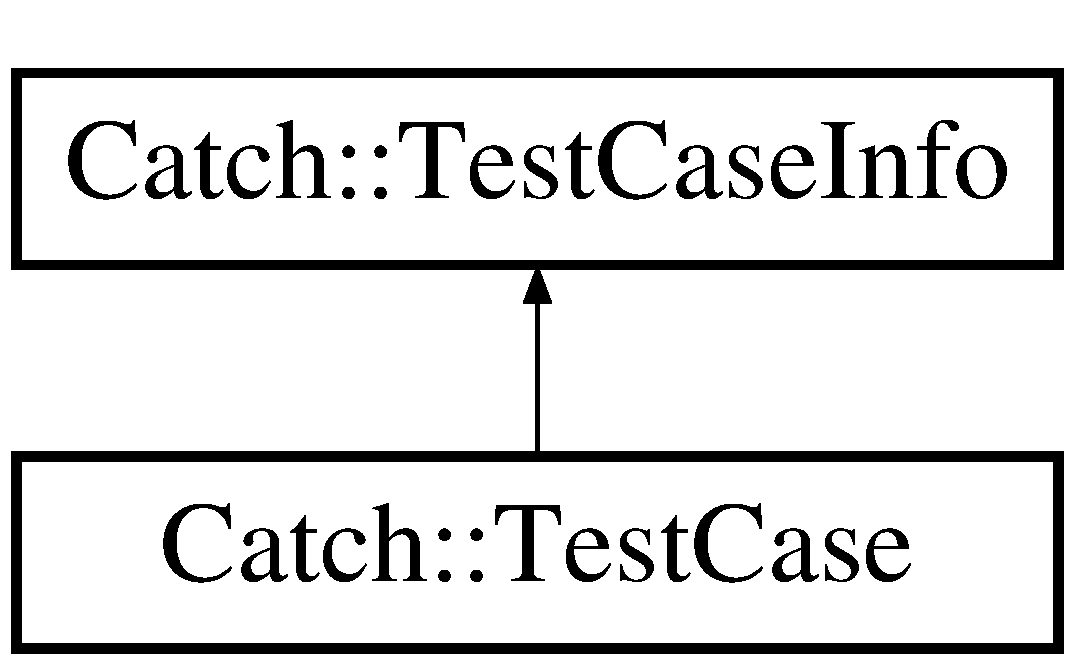
\includegraphics[height=2.000000cm]{structCatch_1_1TestCaseInfo}
\end{center}
\end{figure}
\subsection*{Public Types}
\begin{DoxyCompactItemize}
\item 
enum \hyperlink{structCatch_1_1TestCaseInfo_a39b232f74b4a7a6f2183b96759027eac}{Special\-Properties} \{ \\*
\hyperlink{structCatch_1_1TestCaseInfo_a39b232f74b4a7a6f2183b96759027eacaf94e9de5f8ec1e53b1aa761ec564b31a}{None} = 0, 
\hyperlink{structCatch_1_1TestCaseInfo_a39b232f74b4a7a6f2183b96759027eacaeda53906c14c3973e0980900c132b8f7}{Is\-Hidden} = 1 $<$$<$ 1, 
\hyperlink{structCatch_1_1TestCaseInfo_a39b232f74b4a7a6f2183b96759027eacaf9002285bccfc343935958f3953f4c01}{Should\-Fail} = 1 $<$$<$ 2, 
\hyperlink{structCatch_1_1TestCaseInfo_a39b232f74b4a7a6f2183b96759027eacadf1873d3271121cb9f52d7df45b416ca}{May\-Fail} = 1 $<$$<$ 3, 
\\*
\hyperlink{structCatch_1_1TestCaseInfo_a39b232f74b4a7a6f2183b96759027eaca4704adf89ed7f7ad653d08f99813a974}{Throws} = 1 $<$$<$ 4, 
\hyperlink{structCatch_1_1TestCaseInfo_a39b232f74b4a7a6f2183b96759027eaca06472887b53fda9eb8015d74e7fd2cf1}{Non\-Portable} = 1 $<$$<$ 5
 \}
\end{DoxyCompactItemize}
\subsection*{Public Member Functions}
\begin{DoxyCompactItemize}
\item 
\hyperlink{structCatch_1_1TestCaseInfo_a35ec65315e0d1f178491b5a59f3f3123}{Test\-Case\-Info} (std\-::string const \&\-\_\-name, std\-::string const \&\-\_\-class\-Name, std\-::string const \&\-\_\-description, std\-::set$<$ std\-::string $>$ const \&\-\_\-tags, \hyperlink{structCatch_1_1SourceLineInfo}{Source\-Line\-Info} const \&\-\_\-line\-Info)
\item 
\hyperlink{structCatch_1_1TestCaseInfo_ac338adb4e38f4bf3977fb45b2b1fe447}{Test\-Case\-Info} (\hyperlink{structCatch_1_1TestCaseInfo}{Test\-Case\-Info} const \&other)
\item 
bool \hyperlink{structCatch_1_1TestCaseInfo_a01ac8b11d8c105e5278a239ab5214257}{is\-Hidden} () const 
\item 
bool \hyperlink{structCatch_1_1TestCaseInfo_a19fb4f0b755956eee8a1fecf713fb7ca}{throws} () const 
\item 
bool \hyperlink{structCatch_1_1TestCaseInfo_a64586336bb49bd6e9ef8a089b072a712}{ok\-To\-Fail} () const 
\item 
bool \hyperlink{structCatch_1_1TestCaseInfo_a1ed1c3689c2874c421466945bd3cb75c}{expected\-To\-Fail} () const 
\end{DoxyCompactItemize}
\subsection*{Public Attributes}
\begin{DoxyCompactItemize}
\item 
std\-::string \hyperlink{structCatch_1_1TestCaseInfo_a463794e2f5cfead307c93efd134ade36}{name}
\item 
std\-::string \hyperlink{structCatch_1_1TestCaseInfo_a1a5e0825132a38d091defdebbf2f8ce9}{class\-Name}
\item 
std\-::string \hyperlink{structCatch_1_1TestCaseInfo_a37fe2db9425bc45f6a33893eac31198e}{description}
\item 
std\-::set$<$ std\-::string $>$ \hyperlink{structCatch_1_1TestCaseInfo_a045f62e7719a8760a5b456f7fd2dc97c}{tags}
\item 
std\-::set$<$ std\-::string $>$ \hyperlink{structCatch_1_1TestCaseInfo_a0ed3864a313e8ddc3ae38431be5be9ae}{lcase\-Tags}
\item 
std\-::string \hyperlink{structCatch_1_1TestCaseInfo_ac65c2d36fd36f71e9bf782b2ea245c64}{tags\-As\-String}
\item 
\hyperlink{structCatch_1_1SourceLineInfo}{Source\-Line\-Info} \hyperlink{structCatch_1_1TestCaseInfo_aa9407b7f442655b51a2aad24b3fa2fd3}{line\-Info}
\item 
\hyperlink{structCatch_1_1TestCaseInfo_a39b232f74b4a7a6f2183b96759027eac}{Special\-Properties} \hyperlink{structCatch_1_1TestCaseInfo_afc1e84bd7a2e180895a06d9131302af0}{properties}
\end{DoxyCompactItemize}
\subsection*{Friends}
\begin{DoxyCompactItemize}
\item 
void \hyperlink{structCatch_1_1TestCaseInfo_addc10c770e56f49da5baa0c76cf25bd5}{set\-Tags} (\hyperlink{structCatch_1_1TestCaseInfo}{Test\-Case\-Info} \&test\-Case\-Info, std\-::set$<$ std\-::string $>$ const \&\hyperlink{structCatch_1_1TestCaseInfo_a045f62e7719a8760a5b456f7fd2dc97c}{tags})
\end{DoxyCompactItemize}


\subsection{Member Enumeration Documentation}
\hypertarget{structCatch_1_1TestCaseInfo_a39b232f74b4a7a6f2183b96759027eac}{\index{Catch\-::\-Test\-Case\-Info@{Catch\-::\-Test\-Case\-Info}!Special\-Properties@{Special\-Properties}}
\index{Special\-Properties@{Special\-Properties}!Catch::TestCaseInfo@{Catch\-::\-Test\-Case\-Info}}
\subsubsection[{Special\-Properties}]{\setlength{\rightskip}{0pt plus 5cm}enum {\bf Catch\-::\-Test\-Case\-Info\-::\-Special\-Properties}}}\label{structCatch_1_1TestCaseInfo_a39b232f74b4a7a6f2183b96759027eac}
\begin{Desc}
\item[Enumerator]\par
\begin{description}
\index{None@{None}!Catch\-::\-Test\-Case\-Info@{Catch\-::\-Test\-Case\-Info}}\index{Catch\-::\-Test\-Case\-Info@{Catch\-::\-Test\-Case\-Info}!None@{None}}\item[{\em 
\hypertarget{structCatch_1_1TestCaseInfo_a39b232f74b4a7a6f2183b96759027eacaf94e9de5f8ec1e53b1aa761ec564b31a}{None}\label{structCatch_1_1TestCaseInfo_a39b232f74b4a7a6f2183b96759027eacaf94e9de5f8ec1e53b1aa761ec564b31a}
}]\index{Is\-Hidden@{Is\-Hidden}!Catch\-::\-Test\-Case\-Info@{Catch\-::\-Test\-Case\-Info}}\index{Catch\-::\-Test\-Case\-Info@{Catch\-::\-Test\-Case\-Info}!Is\-Hidden@{Is\-Hidden}}\item[{\em 
\hypertarget{structCatch_1_1TestCaseInfo_a39b232f74b4a7a6f2183b96759027eacaeda53906c14c3973e0980900c132b8f7}{Is\-Hidden}\label{structCatch_1_1TestCaseInfo_a39b232f74b4a7a6f2183b96759027eacaeda53906c14c3973e0980900c132b8f7}
}]\index{Should\-Fail@{Should\-Fail}!Catch\-::\-Test\-Case\-Info@{Catch\-::\-Test\-Case\-Info}}\index{Catch\-::\-Test\-Case\-Info@{Catch\-::\-Test\-Case\-Info}!Should\-Fail@{Should\-Fail}}\item[{\em 
\hypertarget{structCatch_1_1TestCaseInfo_a39b232f74b4a7a6f2183b96759027eacaf9002285bccfc343935958f3953f4c01}{Should\-Fail}\label{structCatch_1_1TestCaseInfo_a39b232f74b4a7a6f2183b96759027eacaf9002285bccfc343935958f3953f4c01}
}]\index{May\-Fail@{May\-Fail}!Catch\-::\-Test\-Case\-Info@{Catch\-::\-Test\-Case\-Info}}\index{Catch\-::\-Test\-Case\-Info@{Catch\-::\-Test\-Case\-Info}!May\-Fail@{May\-Fail}}\item[{\em 
\hypertarget{structCatch_1_1TestCaseInfo_a39b232f74b4a7a6f2183b96759027eacadf1873d3271121cb9f52d7df45b416ca}{May\-Fail}\label{structCatch_1_1TestCaseInfo_a39b232f74b4a7a6f2183b96759027eacadf1873d3271121cb9f52d7df45b416ca}
}]\index{Throws@{Throws}!Catch\-::\-Test\-Case\-Info@{Catch\-::\-Test\-Case\-Info}}\index{Catch\-::\-Test\-Case\-Info@{Catch\-::\-Test\-Case\-Info}!Throws@{Throws}}\item[{\em 
\hypertarget{structCatch_1_1TestCaseInfo_a39b232f74b4a7a6f2183b96759027eaca4704adf89ed7f7ad653d08f99813a974}{Throws}\label{structCatch_1_1TestCaseInfo_a39b232f74b4a7a6f2183b96759027eaca4704adf89ed7f7ad653d08f99813a974}
}]\index{Non\-Portable@{Non\-Portable}!Catch\-::\-Test\-Case\-Info@{Catch\-::\-Test\-Case\-Info}}\index{Catch\-::\-Test\-Case\-Info@{Catch\-::\-Test\-Case\-Info}!Non\-Portable@{Non\-Portable}}\item[{\em 
\hypertarget{structCatch_1_1TestCaseInfo_a39b232f74b4a7a6f2183b96759027eaca06472887b53fda9eb8015d74e7fd2cf1}{Non\-Portable}\label{structCatch_1_1TestCaseInfo_a39b232f74b4a7a6f2183b96759027eaca06472887b53fda9eb8015d74e7fd2cf1}
}]\end{description}
\end{Desc}


\subsection{Constructor \& Destructor Documentation}
\hypertarget{structCatch_1_1TestCaseInfo_a35ec65315e0d1f178491b5a59f3f3123}{\index{Catch\-::\-Test\-Case\-Info@{Catch\-::\-Test\-Case\-Info}!Test\-Case\-Info@{Test\-Case\-Info}}
\index{Test\-Case\-Info@{Test\-Case\-Info}!Catch::TestCaseInfo@{Catch\-::\-Test\-Case\-Info}}
\subsubsection[{Test\-Case\-Info}]{\setlength{\rightskip}{0pt plus 5cm}Catch\-::\-Test\-Case\-Info\-::\-Test\-Case\-Info (
\begin{DoxyParamCaption}
\item[{std\-::string const \&}]{\-\_\-name, }
\item[{std\-::string const \&}]{\-\_\-class\-Name, }
\item[{std\-::string const \&}]{\-\_\-description, }
\item[{std\-::set$<$ std\-::string $>$ const \&}]{\-\_\-tags, }
\item[{{\bf Source\-Line\-Info} const \&}]{\-\_\-line\-Info}
\end{DoxyParamCaption}
)}}\label{structCatch_1_1TestCaseInfo_a35ec65315e0d1f178491b5a59f3f3123}
\hypertarget{structCatch_1_1TestCaseInfo_ac338adb4e38f4bf3977fb45b2b1fe447}{\index{Catch\-::\-Test\-Case\-Info@{Catch\-::\-Test\-Case\-Info}!Test\-Case\-Info@{Test\-Case\-Info}}
\index{Test\-Case\-Info@{Test\-Case\-Info}!Catch::TestCaseInfo@{Catch\-::\-Test\-Case\-Info}}
\subsubsection[{Test\-Case\-Info}]{\setlength{\rightskip}{0pt plus 5cm}Catch\-::\-Test\-Case\-Info\-::\-Test\-Case\-Info (
\begin{DoxyParamCaption}
\item[{{\bf Test\-Case\-Info} const \&}]{other}
\end{DoxyParamCaption}
)}}\label{structCatch_1_1TestCaseInfo_ac338adb4e38f4bf3977fb45b2b1fe447}


\subsection{Member Function Documentation}
\hypertarget{structCatch_1_1TestCaseInfo_a1ed1c3689c2874c421466945bd3cb75c}{\index{Catch\-::\-Test\-Case\-Info@{Catch\-::\-Test\-Case\-Info}!expected\-To\-Fail@{expected\-To\-Fail}}
\index{expected\-To\-Fail@{expected\-To\-Fail}!Catch::TestCaseInfo@{Catch\-::\-Test\-Case\-Info}}
\subsubsection[{expected\-To\-Fail}]{\setlength{\rightskip}{0pt plus 5cm}bool Catch\-::\-Test\-Case\-Info\-::expected\-To\-Fail (
\begin{DoxyParamCaption}
{}
\end{DoxyParamCaption}
) const}}\label{structCatch_1_1TestCaseInfo_a1ed1c3689c2874c421466945bd3cb75c}
\hypertarget{structCatch_1_1TestCaseInfo_a01ac8b11d8c105e5278a239ab5214257}{\index{Catch\-::\-Test\-Case\-Info@{Catch\-::\-Test\-Case\-Info}!is\-Hidden@{is\-Hidden}}
\index{is\-Hidden@{is\-Hidden}!Catch::TestCaseInfo@{Catch\-::\-Test\-Case\-Info}}
\subsubsection[{is\-Hidden}]{\setlength{\rightskip}{0pt plus 5cm}bool Catch\-::\-Test\-Case\-Info\-::is\-Hidden (
\begin{DoxyParamCaption}
{}
\end{DoxyParamCaption}
) const}}\label{structCatch_1_1TestCaseInfo_a01ac8b11d8c105e5278a239ab5214257}
\hypertarget{structCatch_1_1TestCaseInfo_a64586336bb49bd6e9ef8a089b072a712}{\index{Catch\-::\-Test\-Case\-Info@{Catch\-::\-Test\-Case\-Info}!ok\-To\-Fail@{ok\-To\-Fail}}
\index{ok\-To\-Fail@{ok\-To\-Fail}!Catch::TestCaseInfo@{Catch\-::\-Test\-Case\-Info}}
\subsubsection[{ok\-To\-Fail}]{\setlength{\rightskip}{0pt plus 5cm}bool Catch\-::\-Test\-Case\-Info\-::ok\-To\-Fail (
\begin{DoxyParamCaption}
{}
\end{DoxyParamCaption}
) const}}\label{structCatch_1_1TestCaseInfo_a64586336bb49bd6e9ef8a089b072a712}
\hypertarget{structCatch_1_1TestCaseInfo_a19fb4f0b755956eee8a1fecf713fb7ca}{\index{Catch\-::\-Test\-Case\-Info@{Catch\-::\-Test\-Case\-Info}!throws@{throws}}
\index{throws@{throws}!Catch::TestCaseInfo@{Catch\-::\-Test\-Case\-Info}}
\subsubsection[{throws}]{\setlength{\rightskip}{0pt plus 5cm}bool Catch\-::\-Test\-Case\-Info\-::throws (
\begin{DoxyParamCaption}
{}
\end{DoxyParamCaption}
) const}}\label{structCatch_1_1TestCaseInfo_a19fb4f0b755956eee8a1fecf713fb7ca}


\subsection{Friends And Related Function Documentation}
\hypertarget{structCatch_1_1TestCaseInfo_addc10c770e56f49da5baa0c76cf25bd5}{\index{Catch\-::\-Test\-Case\-Info@{Catch\-::\-Test\-Case\-Info}!set\-Tags@{set\-Tags}}
\index{set\-Tags@{set\-Tags}!Catch::TestCaseInfo@{Catch\-::\-Test\-Case\-Info}}
\subsubsection[{set\-Tags}]{\setlength{\rightskip}{0pt plus 5cm}void set\-Tags (
\begin{DoxyParamCaption}
\item[{{\bf Test\-Case\-Info} \&}]{test\-Case\-Info, }
\item[{std\-::set$<$ std\-::string $>$ const \&}]{tags}
\end{DoxyParamCaption}
)\hspace{0.3cm}{\ttfamily [friend]}}}\label{structCatch_1_1TestCaseInfo_addc10c770e56f49da5baa0c76cf25bd5}


\subsection{Member Data Documentation}
\hypertarget{structCatch_1_1TestCaseInfo_a1a5e0825132a38d091defdebbf2f8ce9}{\index{Catch\-::\-Test\-Case\-Info@{Catch\-::\-Test\-Case\-Info}!class\-Name@{class\-Name}}
\index{class\-Name@{class\-Name}!Catch::TestCaseInfo@{Catch\-::\-Test\-Case\-Info}}
\subsubsection[{class\-Name}]{\setlength{\rightskip}{0pt plus 5cm}std\-::string Catch\-::\-Test\-Case\-Info\-::class\-Name}}\label{structCatch_1_1TestCaseInfo_a1a5e0825132a38d091defdebbf2f8ce9}
\hypertarget{structCatch_1_1TestCaseInfo_a37fe2db9425bc45f6a33893eac31198e}{\index{Catch\-::\-Test\-Case\-Info@{Catch\-::\-Test\-Case\-Info}!description@{description}}
\index{description@{description}!Catch::TestCaseInfo@{Catch\-::\-Test\-Case\-Info}}
\subsubsection[{description}]{\setlength{\rightskip}{0pt plus 5cm}std\-::string Catch\-::\-Test\-Case\-Info\-::description}}\label{structCatch_1_1TestCaseInfo_a37fe2db9425bc45f6a33893eac31198e}
\hypertarget{structCatch_1_1TestCaseInfo_a0ed3864a313e8ddc3ae38431be5be9ae}{\index{Catch\-::\-Test\-Case\-Info@{Catch\-::\-Test\-Case\-Info}!lcase\-Tags@{lcase\-Tags}}
\index{lcase\-Tags@{lcase\-Tags}!Catch::TestCaseInfo@{Catch\-::\-Test\-Case\-Info}}
\subsubsection[{lcase\-Tags}]{\setlength{\rightskip}{0pt plus 5cm}std\-::set$<$std\-::string$>$ Catch\-::\-Test\-Case\-Info\-::lcase\-Tags}}\label{structCatch_1_1TestCaseInfo_a0ed3864a313e8ddc3ae38431be5be9ae}
\hypertarget{structCatch_1_1TestCaseInfo_aa9407b7f442655b51a2aad24b3fa2fd3}{\index{Catch\-::\-Test\-Case\-Info@{Catch\-::\-Test\-Case\-Info}!line\-Info@{line\-Info}}
\index{line\-Info@{line\-Info}!Catch::TestCaseInfo@{Catch\-::\-Test\-Case\-Info}}
\subsubsection[{line\-Info}]{\setlength{\rightskip}{0pt plus 5cm}{\bf Source\-Line\-Info} Catch\-::\-Test\-Case\-Info\-::line\-Info}}\label{structCatch_1_1TestCaseInfo_aa9407b7f442655b51a2aad24b3fa2fd3}
\hypertarget{structCatch_1_1TestCaseInfo_a463794e2f5cfead307c93efd134ade36}{\index{Catch\-::\-Test\-Case\-Info@{Catch\-::\-Test\-Case\-Info}!name@{name}}
\index{name@{name}!Catch::TestCaseInfo@{Catch\-::\-Test\-Case\-Info}}
\subsubsection[{name}]{\setlength{\rightskip}{0pt plus 5cm}std\-::string Catch\-::\-Test\-Case\-Info\-::name}}\label{structCatch_1_1TestCaseInfo_a463794e2f5cfead307c93efd134ade36}
\hypertarget{structCatch_1_1TestCaseInfo_afc1e84bd7a2e180895a06d9131302af0}{\index{Catch\-::\-Test\-Case\-Info@{Catch\-::\-Test\-Case\-Info}!properties@{properties}}
\index{properties@{properties}!Catch::TestCaseInfo@{Catch\-::\-Test\-Case\-Info}}
\subsubsection[{properties}]{\setlength{\rightskip}{0pt plus 5cm}{\bf Special\-Properties} Catch\-::\-Test\-Case\-Info\-::properties}}\label{structCatch_1_1TestCaseInfo_afc1e84bd7a2e180895a06d9131302af0}
\hypertarget{structCatch_1_1TestCaseInfo_a045f62e7719a8760a5b456f7fd2dc97c}{\index{Catch\-::\-Test\-Case\-Info@{Catch\-::\-Test\-Case\-Info}!tags@{tags}}
\index{tags@{tags}!Catch::TestCaseInfo@{Catch\-::\-Test\-Case\-Info}}
\subsubsection[{tags}]{\setlength{\rightskip}{0pt plus 5cm}std\-::set$<$std\-::string$>$ Catch\-::\-Test\-Case\-Info\-::tags}}\label{structCatch_1_1TestCaseInfo_a045f62e7719a8760a5b456f7fd2dc97c}
\hypertarget{structCatch_1_1TestCaseInfo_ac65c2d36fd36f71e9bf782b2ea245c64}{\index{Catch\-::\-Test\-Case\-Info@{Catch\-::\-Test\-Case\-Info}!tags\-As\-String@{tags\-As\-String}}
\index{tags\-As\-String@{tags\-As\-String}!Catch::TestCaseInfo@{Catch\-::\-Test\-Case\-Info}}
\subsubsection[{tags\-As\-String}]{\setlength{\rightskip}{0pt plus 5cm}std\-::string Catch\-::\-Test\-Case\-Info\-::tags\-As\-String}}\label{structCatch_1_1TestCaseInfo_ac65c2d36fd36f71e9bf782b2ea245c64}


The documentation for this struct was generated from the following file\-:\begin{DoxyCompactItemize}
\item 
/home/alexander/\-Un\-B/\-M\-P/\-Trabalho\-\_\-2\-\_\-\-M\-P\-\_\-\-Alexander\-\_\-13\-\_\-0039853/include/\hyperlink{catch_8hpp}{catch.\-hpp}\end{DoxyCompactItemize}

\hypertarget{structCatch_1_1TestFailureException}{\section{Catch\-:\-:Test\-Failure\-Exception Struct Reference}
\label{structCatch_1_1TestFailureException}\index{Catch\-::\-Test\-Failure\-Exception@{Catch\-::\-Test\-Failure\-Exception}}
}


{\ttfamily \#include $<$catch.\-hpp$>$}



The documentation for this struct was generated from the following file\-:\begin{DoxyCompactItemize}
\item 
/home/alexander/\-Un\-B/\-M\-P/\-Trabalho\-\_\-2\-\_\-\-M\-P\-\_\-\-Alexander\-\_\-13\-\_\-0039853/include/\hyperlink{catch_8hpp}{catch.\-hpp}\end{DoxyCompactItemize}

\hypertarget{classCatch_1_1Timer}{\section{Catch\-:\-:Timer Class Reference}
\label{classCatch_1_1Timer}\index{Catch\-::\-Timer@{Catch\-::\-Timer}}
}


{\ttfamily \#include $<$catch.\-hpp$>$}

\subsection*{Public Member Functions}
\begin{DoxyCompactItemize}
\item 
\hyperlink{classCatch_1_1Timer_af09b7cd7a40af71f4704262afb31558a}{Timer} ()
\item 
void \hyperlink{classCatch_1_1Timer_a0a56e879e43f36c102bf9ea8b5fc8b72}{start} ()
\item 
unsigned int \hyperlink{classCatch_1_1Timer_a4b0062f169f7d3150b0e8073ab37890a}{get\-Elapsed\-Microseconds} () const 
\item 
unsigned int \hyperlink{classCatch_1_1Timer_a4cf3f9fbee9c76e87d989d9bc6913b68}{get\-Elapsed\-Milliseconds} () const 
\item 
double \hyperlink{classCatch_1_1Timer_a8500ef3481a9bf6ae81337972d9f95a3}{get\-Elapsed\-Seconds} () const 
\end{DoxyCompactItemize}


\subsection{Constructor \& Destructor Documentation}
\hypertarget{classCatch_1_1Timer_af09b7cd7a40af71f4704262afb31558a}{\index{Catch\-::\-Timer@{Catch\-::\-Timer}!Timer@{Timer}}
\index{Timer@{Timer}!Catch::Timer@{Catch\-::\-Timer}}
\subsubsection[{Timer}]{\setlength{\rightskip}{0pt plus 5cm}Catch\-::\-Timer\-::\-Timer (
\begin{DoxyParamCaption}
{}
\end{DoxyParamCaption}
)\hspace{0.3cm}{\ttfamily [inline]}}}\label{classCatch_1_1Timer_af09b7cd7a40af71f4704262afb31558a}


\subsection{Member Function Documentation}
\hypertarget{classCatch_1_1Timer_a4b0062f169f7d3150b0e8073ab37890a}{\index{Catch\-::\-Timer@{Catch\-::\-Timer}!get\-Elapsed\-Microseconds@{get\-Elapsed\-Microseconds}}
\index{get\-Elapsed\-Microseconds@{get\-Elapsed\-Microseconds}!Catch::Timer@{Catch\-::\-Timer}}
\subsubsection[{get\-Elapsed\-Microseconds}]{\setlength{\rightskip}{0pt plus 5cm}unsigned int Catch\-::\-Timer\-::get\-Elapsed\-Microseconds (
\begin{DoxyParamCaption}
{}
\end{DoxyParamCaption}
) const}}\label{classCatch_1_1Timer_a4b0062f169f7d3150b0e8073ab37890a}
\hypertarget{classCatch_1_1Timer_a4cf3f9fbee9c76e87d989d9bc6913b68}{\index{Catch\-::\-Timer@{Catch\-::\-Timer}!get\-Elapsed\-Milliseconds@{get\-Elapsed\-Milliseconds}}
\index{get\-Elapsed\-Milliseconds@{get\-Elapsed\-Milliseconds}!Catch::Timer@{Catch\-::\-Timer}}
\subsubsection[{get\-Elapsed\-Milliseconds}]{\setlength{\rightskip}{0pt plus 5cm}unsigned int Catch\-::\-Timer\-::get\-Elapsed\-Milliseconds (
\begin{DoxyParamCaption}
{}
\end{DoxyParamCaption}
) const}}\label{classCatch_1_1Timer_a4cf3f9fbee9c76e87d989d9bc6913b68}
\hypertarget{classCatch_1_1Timer_a8500ef3481a9bf6ae81337972d9f95a3}{\index{Catch\-::\-Timer@{Catch\-::\-Timer}!get\-Elapsed\-Seconds@{get\-Elapsed\-Seconds}}
\index{get\-Elapsed\-Seconds@{get\-Elapsed\-Seconds}!Catch::Timer@{Catch\-::\-Timer}}
\subsubsection[{get\-Elapsed\-Seconds}]{\setlength{\rightskip}{0pt plus 5cm}double Catch\-::\-Timer\-::get\-Elapsed\-Seconds (
\begin{DoxyParamCaption}
{}
\end{DoxyParamCaption}
) const}}\label{classCatch_1_1Timer_a8500ef3481a9bf6ae81337972d9f95a3}
\hypertarget{classCatch_1_1Timer_a0a56e879e43f36c102bf9ea8b5fc8b72}{\index{Catch\-::\-Timer@{Catch\-::\-Timer}!start@{start}}
\index{start@{start}!Catch::Timer@{Catch\-::\-Timer}}
\subsubsection[{start}]{\setlength{\rightskip}{0pt plus 5cm}void Catch\-::\-Timer\-::start (
\begin{DoxyParamCaption}
{}
\end{DoxyParamCaption}
)}}\label{classCatch_1_1Timer_a0a56e879e43f36c102bf9ea8b5fc8b72}


The documentation for this class was generated from the following file\-:\begin{DoxyCompactItemize}
\item 
/home/alexander/\-Un\-B/\-M\-P/\-Trabalho\-\_\-2\-\_\-\-M\-P\-\_\-\-Alexander\-\_\-13\-\_\-0039853/include/\hyperlink{catch_8hpp}{catch.\-hpp}\end{DoxyCompactItemize}

\hypertarget{structCatch_1_1Totals}{\section{Catch\-:\-:Totals Struct Reference}
\label{structCatch_1_1Totals}\index{Catch\-::\-Totals@{Catch\-::\-Totals}}
}


{\ttfamily \#include $<$catch.\-hpp$>$}

\subsection*{Public Member Functions}
\begin{DoxyCompactItemize}
\item 
\hyperlink{structCatch_1_1Totals}{Totals} \hyperlink{structCatch_1_1Totals_abe15cd8a82ba9a4868dd7a542add827c}{operator-\/} (\hyperlink{structCatch_1_1Totals}{Totals} const \&other) const 
\item 
\hyperlink{structCatch_1_1Totals}{Totals} \hyperlink{structCatch_1_1Totals_a3dee0f599c081a8360c0112fb1dafe8f}{delta} (\hyperlink{structCatch_1_1Totals}{Totals} const \&prev\-Totals) const 
\item 
\hyperlink{structCatch_1_1Totals}{Totals} \& \hyperlink{structCatch_1_1Totals_a574015076e54cc405c70b053e3356e43}{operator+=} (\hyperlink{structCatch_1_1Totals}{Totals} const \&other)
\end{DoxyCompactItemize}
\subsection*{Public Attributes}
\begin{DoxyCompactItemize}
\item 
\hyperlink{structCatch_1_1Counts}{Counts} \hyperlink{structCatch_1_1Totals_a885ded66df752147b30c3d45aa602ec9}{assertions}
\item 
\hyperlink{structCatch_1_1Counts}{Counts} \hyperlink{structCatch_1_1Totals_adb195fe477aedee2ecea88c888f16506}{test\-Cases}
\end{DoxyCompactItemize}


\subsection{Member Function Documentation}
\hypertarget{structCatch_1_1Totals_a3dee0f599c081a8360c0112fb1dafe8f}{\index{Catch\-::\-Totals@{Catch\-::\-Totals}!delta@{delta}}
\index{delta@{delta}!Catch::Totals@{Catch\-::\-Totals}}
\subsubsection[{delta}]{\setlength{\rightskip}{0pt plus 5cm}{\bf Totals} Catch\-::\-Totals\-::delta (
\begin{DoxyParamCaption}
\item[{{\bf Totals} const \&}]{prev\-Totals}
\end{DoxyParamCaption}
) const\hspace{0.3cm}{\ttfamily [inline]}}}\label{structCatch_1_1Totals_a3dee0f599c081a8360c0112fb1dafe8f}
\hypertarget{structCatch_1_1Totals_a574015076e54cc405c70b053e3356e43}{\index{Catch\-::\-Totals@{Catch\-::\-Totals}!operator+=@{operator+=}}
\index{operator+=@{operator+=}!Catch::Totals@{Catch\-::\-Totals}}
\subsubsection[{operator+=}]{\setlength{\rightskip}{0pt plus 5cm}{\bf Totals}\& Catch\-::\-Totals\-::operator+= (
\begin{DoxyParamCaption}
\item[{{\bf Totals} const \&}]{other}
\end{DoxyParamCaption}
)\hspace{0.3cm}{\ttfamily [inline]}}}\label{structCatch_1_1Totals_a574015076e54cc405c70b053e3356e43}
\hypertarget{structCatch_1_1Totals_abe15cd8a82ba9a4868dd7a542add827c}{\index{Catch\-::\-Totals@{Catch\-::\-Totals}!operator-\/@{operator-\/}}
\index{operator-\/@{operator-\/}!Catch::Totals@{Catch\-::\-Totals}}
\subsubsection[{operator-\/}]{\setlength{\rightskip}{0pt plus 5cm}{\bf Totals} Catch\-::\-Totals\-::operator-\/ (
\begin{DoxyParamCaption}
\item[{{\bf Totals} const \&}]{other}
\end{DoxyParamCaption}
) const\hspace{0.3cm}{\ttfamily [inline]}}}\label{structCatch_1_1Totals_abe15cd8a82ba9a4868dd7a542add827c}


\subsection{Member Data Documentation}
\hypertarget{structCatch_1_1Totals_a885ded66df752147b30c3d45aa602ec9}{\index{Catch\-::\-Totals@{Catch\-::\-Totals}!assertions@{assertions}}
\index{assertions@{assertions}!Catch::Totals@{Catch\-::\-Totals}}
\subsubsection[{assertions}]{\setlength{\rightskip}{0pt plus 5cm}{\bf Counts} Catch\-::\-Totals\-::assertions}}\label{structCatch_1_1Totals_a885ded66df752147b30c3d45aa602ec9}
\hypertarget{structCatch_1_1Totals_adb195fe477aedee2ecea88c888f16506}{\index{Catch\-::\-Totals@{Catch\-::\-Totals}!test\-Cases@{test\-Cases}}
\index{test\-Cases@{test\-Cases}!Catch::Totals@{Catch\-::\-Totals}}
\subsubsection[{test\-Cases}]{\setlength{\rightskip}{0pt plus 5cm}{\bf Counts} Catch\-::\-Totals\-::test\-Cases}}\label{structCatch_1_1Totals_adb195fe477aedee2ecea88c888f16506}


The documentation for this struct was generated from the following file\-:\begin{DoxyCompactItemize}
\item 
/home/alexander/\-Un\-B/\-M\-P/\-Trabalho\-\_\-2\-\_\-\-M\-P\-\_\-\-Alexander\-\_\-13\-\_\-0039853/include/\hyperlink{catch_8hpp}{catch.\-hpp}\end{DoxyCompactItemize}

\hypertarget{structCatch_1_1Detail_1_1TrueType}{\section{Catch\-:\-:Detail\-:\-:True\-Type Struct Reference}
\label{structCatch_1_1Detail_1_1TrueType}\index{Catch\-::\-Detail\-::\-True\-Type@{Catch\-::\-Detail\-::\-True\-Type}}
}


{\ttfamily \#include $<$catch.\-hpp$>$}

\subsection*{Public Attributes}
\begin{DoxyCompactItemize}
\item 
char \hyperlink{structCatch_1_1Detail_1_1TrueType_a3aaaeb75909e668b293c8a81f5fb6419}{sizer} \mbox{[}1\mbox{]}
\end{DoxyCompactItemize}


\subsection{Member Data Documentation}
\hypertarget{structCatch_1_1Detail_1_1TrueType_a3aaaeb75909e668b293c8a81f5fb6419}{\index{Catch\-::\-Detail\-::\-True\-Type@{Catch\-::\-Detail\-::\-True\-Type}!sizer@{sizer}}
\index{sizer@{sizer}!Catch::Detail::TrueType@{Catch\-::\-Detail\-::\-True\-Type}}
\subsubsection[{sizer}]{\setlength{\rightskip}{0pt plus 5cm}char Catch\-::\-Detail\-::\-True\-Type\-::sizer\mbox{[}1\mbox{]}}}\label{structCatch_1_1Detail_1_1TrueType_a3aaaeb75909e668b293c8a81f5fb6419}


The documentation for this struct was generated from the following file\-:\begin{DoxyCompactItemize}
\item 
/home/alexander/\-Un\-B/\-M\-P/\-Trabalho\-\_\-2\-\_\-\-M\-P\-\_\-\-Alexander\-\_\-13\-\_\-0039853/include/\hyperlink{catch_8hpp}{catch.\-hpp}\end{DoxyCompactItemize}

\hypertarget{classCatch_1_1ValuesGenerator}{\section{Catch\-:\-:Values\-Generator$<$ T $>$ Class Template Reference}
\label{classCatch_1_1ValuesGenerator}\index{Catch\-::\-Values\-Generator$<$ T $>$@{Catch\-::\-Values\-Generator$<$ T $>$}}
}


{\ttfamily \#include $<$catch.\-hpp$>$}

Inheritance diagram for Catch\-:\-:Values\-Generator$<$ T $>$\-:\begin{figure}[H]
\begin{center}
\leavevmode
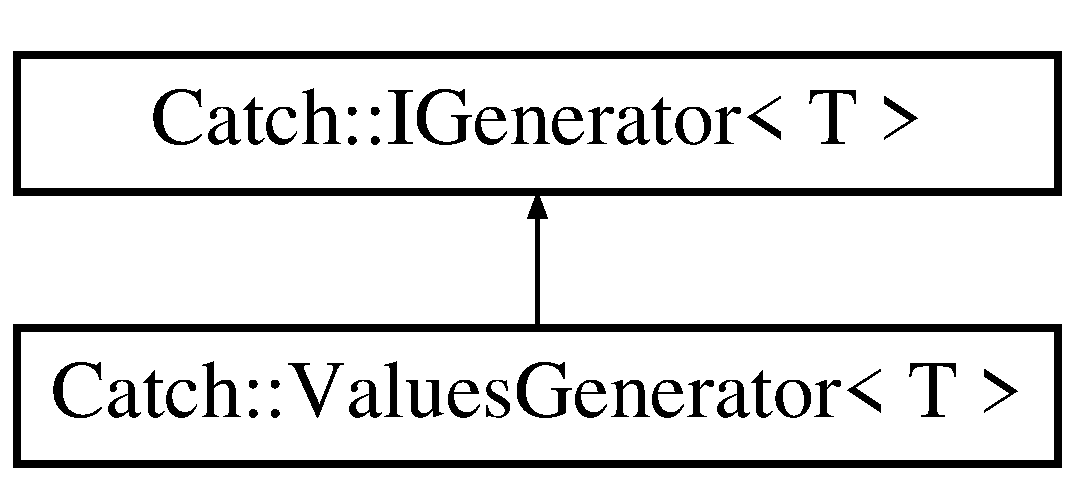
\includegraphics[height=2.000000cm]{classCatch_1_1ValuesGenerator}
\end{center}
\end{figure}
\subsection*{Public Member Functions}
\begin{DoxyCompactItemize}
\item 
\hyperlink{classCatch_1_1ValuesGenerator_a36cd3d75afb1f5502400c3ad7cae7a5e}{Values\-Generator} ()
\item 
void \hyperlink{classCatch_1_1ValuesGenerator_a8412c8ce5d9d4fc6ff06d5246d56d538}{add} (T value)
\item 
virtual T \hyperlink{classCatch_1_1ValuesGenerator_a60599dd67096ff108471f64ee42acd9d}{get\-Value} (std\-::size\-\_\-t index) const 
\item 
virtual std\-::size\-\_\-t \hyperlink{classCatch_1_1ValuesGenerator_a98a80bb0dd682c44e82e4a75e98c4682}{size} () const 
\end{DoxyCompactItemize}


\subsection{Constructor \& Destructor Documentation}
\hypertarget{classCatch_1_1ValuesGenerator_a36cd3d75afb1f5502400c3ad7cae7a5e}{\index{Catch\-::\-Values\-Generator@{Catch\-::\-Values\-Generator}!Values\-Generator@{Values\-Generator}}
\index{Values\-Generator@{Values\-Generator}!Catch::ValuesGenerator@{Catch\-::\-Values\-Generator}}
\subsubsection[{Values\-Generator}]{\setlength{\rightskip}{0pt plus 5cm}template$<$typename T$>$ {\bf Catch\-::\-Values\-Generator}$<$ T $>$\-::{\bf Values\-Generator} (
\begin{DoxyParamCaption}
{}
\end{DoxyParamCaption}
)\hspace{0.3cm}{\ttfamily [inline]}}}\label{classCatch_1_1ValuesGenerator_a36cd3d75afb1f5502400c3ad7cae7a5e}


\subsection{Member Function Documentation}
\hypertarget{classCatch_1_1ValuesGenerator_a8412c8ce5d9d4fc6ff06d5246d56d538}{\index{Catch\-::\-Values\-Generator@{Catch\-::\-Values\-Generator}!add@{add}}
\index{add@{add}!Catch::ValuesGenerator@{Catch\-::\-Values\-Generator}}
\subsubsection[{add}]{\setlength{\rightskip}{0pt plus 5cm}template$<$typename T$>$ void {\bf Catch\-::\-Values\-Generator}$<$ T $>$\-::add (
\begin{DoxyParamCaption}
\item[{T}]{value}
\end{DoxyParamCaption}
)\hspace{0.3cm}{\ttfamily [inline]}}}\label{classCatch_1_1ValuesGenerator_a8412c8ce5d9d4fc6ff06d5246d56d538}
\hypertarget{classCatch_1_1ValuesGenerator_a60599dd67096ff108471f64ee42acd9d}{\index{Catch\-::\-Values\-Generator@{Catch\-::\-Values\-Generator}!get\-Value@{get\-Value}}
\index{get\-Value@{get\-Value}!Catch::ValuesGenerator@{Catch\-::\-Values\-Generator}}
\subsubsection[{get\-Value}]{\setlength{\rightskip}{0pt plus 5cm}template$<$typename T$>$ virtual T {\bf Catch\-::\-Values\-Generator}$<$ T $>$\-::get\-Value (
\begin{DoxyParamCaption}
\item[{std\-::size\-\_\-t}]{index}
\end{DoxyParamCaption}
) const\hspace{0.3cm}{\ttfamily [inline]}, {\ttfamily [virtual]}}}\label{classCatch_1_1ValuesGenerator_a60599dd67096ff108471f64ee42acd9d}


Implements \hyperlink{structCatch_1_1IGenerator_ad69e937cb66dba3ed9429c42abf4fce3}{Catch\-::\-I\-Generator$<$ T $>$}.

\hypertarget{classCatch_1_1ValuesGenerator_a98a80bb0dd682c44e82e4a75e98c4682}{\index{Catch\-::\-Values\-Generator@{Catch\-::\-Values\-Generator}!size@{size}}
\index{size@{size}!Catch::ValuesGenerator@{Catch\-::\-Values\-Generator}}
\subsubsection[{size}]{\setlength{\rightskip}{0pt plus 5cm}template$<$typename T$>$ virtual std\-::size\-\_\-t {\bf Catch\-::\-Values\-Generator}$<$ T $>$\-::size (
\begin{DoxyParamCaption}
{}
\end{DoxyParamCaption}
) const\hspace{0.3cm}{\ttfamily [inline]}, {\ttfamily [virtual]}}}\label{classCatch_1_1ValuesGenerator_a98a80bb0dd682c44e82e4a75e98c4682}


Implements \hyperlink{structCatch_1_1IGenerator_a2e317253b03e838b6065ce69719a198e}{Catch\-::\-I\-Generator$<$ T $>$}.



The documentation for this class was generated from the following file\-:\begin{DoxyCompactItemize}
\item 
/home/alexander/\-Un\-B/\-M\-P/\-Trabalho\-\_\-2\-\_\-\-M\-P\-\_\-\-Alexander\-\_\-13\-\_\-0039853/include/\hyperlink{catch_8hpp}{catch.\-hpp}\end{DoxyCompactItemize}

\chapter{File Documentation}
\hypertarget{catch_8hpp}{\section{/home/alexander/\-Un\-B/\-M\-P/\-Trabalho\-\_\-2\-\_\-\-M\-P\-\_\-\-Alexander\-\_\-13\-\_\-0039853/include/catch.hpp File Reference}
\label{catch_8hpp}\index{/home/alexander/\-Un\-B/\-M\-P/\-Trabalho\-\_\-2\-\_\-\-M\-P\-\_\-\-Alexander\-\_\-13\-\_\-0039853/include/catch.\-hpp@{/home/alexander/\-Un\-B/\-M\-P/\-Trabalho\-\_\-2\-\_\-\-M\-P\-\_\-\-Alexander\-\_\-13\-\_\-0039853/include/catch.\-hpp}}
}
{\ttfamily \#include $<$sstream$>$}\\*
{\ttfamily \#include $<$algorithm$>$}\\*
{\ttfamily \#include $<$string$>$}\\*
{\ttfamily \#include $<$vector$>$}\\*
{\ttfamily \#include $<$cstddef$>$}\\*
{\ttfamily \#include $<$iomanip$>$}\\*
{\ttfamily \#include $<$limits$>$}\\*
{\ttfamily \#include $<$stdint.\-h$>$}\\*
{\ttfamily \#include $<$stdlib.\-h$>$}\\*
{\ttfamily \#include $<$cmath$>$}\\*
{\ttfamily \#include $<$set$>$}\\*
\subsection*{Classes}
\begin{DoxyCompactItemize}
\item 
struct \hyperlink{structCatch_1_1CaseSensitive}{Catch\-::\-Case\-Sensitive}
\item 
class \hyperlink{classCatch_1_1NonCopyable}{Catch\-::\-Non\-Copyable}
\item 
class \hyperlink{classCatch_1_1SafeBool}{Catch\-::\-Safe\-Bool}
\item 
struct \hyperlink{structCatch_1_1pluralise}{Catch\-::pluralise}
\item 
struct \hyperlink{structCatch_1_1SourceLineInfo}{Catch\-::\-Source\-Line\-Info}
\item 
struct \hyperlink{structCatch_1_1StreamEndStop}{Catch\-::\-Stream\-End\-Stop}
\item 
class \hyperlink{classCatch_1_1NotImplementedException}{Catch\-::\-Not\-Implemented\-Exception}
\item 
struct \hyperlink{structCatch_1_1IGeneratorInfo}{Catch\-::\-I\-Generator\-Info}
\item 
struct \hyperlink{structCatch_1_1IGeneratorsForTest}{Catch\-::\-I\-Generators\-For\-Test}
\item 
class \hyperlink{classCatch_1_1Ptr}{Catch\-::\-Ptr$<$ T $>$}
\item 
struct \hyperlink{structCatch_1_1IShared}{Catch\-::\-I\-Shared}
\item 
struct \hyperlink{structCatch_1_1SharedImpl}{Catch\-::\-Shared\-Impl$<$ T $>$}
\item 
struct \hyperlink{structCatch_1_1IContext}{Catch\-::\-I\-Context}
\item 
struct \hyperlink{structCatch_1_1IMutableContext}{Catch\-::\-I\-Mutable\-Context}
\item 
struct \hyperlink{structCatch_1_1ITestCase}{Catch\-::\-I\-Test\-Case}
\item 
struct \hyperlink{structCatch_1_1ITestCaseRegistry}{Catch\-::\-I\-Test\-Case\-Registry}
\item 
class \hyperlink{classCatch_1_1MethodTestCase}{Catch\-::\-Method\-Test\-Case$<$ C $>$}
\item 
struct \hyperlink{structCatch_1_1NameAndDesc}{Catch\-::\-Name\-And\-Desc}
\item 
struct \hyperlink{structCatch_1_1AutoReg}{Catch\-::\-Auto\-Reg}
\item 
struct \hyperlink{structCatch_1_1ResultWas}{Catch\-::\-Result\-Was}
\item 
struct \hyperlink{structCatch_1_1ResultDisposition}{Catch\-::\-Result\-Disposition}
\item 
struct \hyperlink{structCatch_1_1DecomposedExpression}{Catch\-::\-Decomposed\-Expression}
\item 
struct \hyperlink{structCatch_1_1AssertionInfo}{Catch\-::\-Assertion\-Info}
\item 
struct \hyperlink{structCatch_1_1AssertionResultData}{Catch\-::\-Assertion\-Result\-Data}
\item 
class \hyperlink{classCatch_1_1AssertionResult}{Catch\-::\-Assertion\-Result}
\item 
struct \hyperlink{structCatch_1_1Matchers_1_1Impl_1_1MatchAllOf}{Catch\-::\-Matchers\-::\-Impl\-::\-Match\-All\-Of$<$ Arg\-T $>$}
\item 
struct \hyperlink{structCatch_1_1Matchers_1_1Impl_1_1MatchAnyOf}{Catch\-::\-Matchers\-::\-Impl\-::\-Match\-Any\-Of$<$ Arg\-T $>$}
\item 
struct \hyperlink{structCatch_1_1Matchers_1_1Impl_1_1MatchNotOf}{Catch\-::\-Matchers\-::\-Impl\-::\-Match\-Not\-Of$<$ Arg\-T $>$}
\item 
class \hyperlink{classCatch_1_1Matchers_1_1Impl_1_1MatcherUntypedBase}{Catch\-::\-Matchers\-::\-Impl\-::\-Matcher\-Untyped\-Base}
\item 
struct \hyperlink{structCatch_1_1Matchers_1_1Impl_1_1MatcherMethod}{Catch\-::\-Matchers\-::\-Impl\-::\-Matcher\-Method$<$ Object\-T $>$}
\item 
struct \hyperlink{structCatch_1_1Matchers_1_1Impl_1_1MatcherMethod_3_01PtrT_01_5_01_4}{Catch\-::\-Matchers\-::\-Impl\-::\-Matcher\-Method$<$ Ptr\-T $\ast$ $>$}
\item 
struct \hyperlink{structCatch_1_1Matchers_1_1Impl_1_1MatcherBase}{Catch\-::\-Matchers\-::\-Impl\-::\-Matcher\-Base$<$ Object\-T, Comparator\-T $>$}
\item 
struct \hyperlink{structCatch_1_1Matchers_1_1Impl_1_1MatchAllOf}{Catch\-::\-Matchers\-::\-Impl\-::\-Match\-All\-Of$<$ Arg\-T $>$}
\item 
struct \hyperlink{structCatch_1_1Matchers_1_1Impl_1_1MatchAnyOf}{Catch\-::\-Matchers\-::\-Impl\-::\-Match\-Any\-Of$<$ Arg\-T $>$}
\item 
struct \hyperlink{structCatch_1_1Matchers_1_1Impl_1_1MatchNotOf}{Catch\-::\-Matchers\-::\-Impl\-::\-Match\-Not\-Of$<$ Arg\-T $>$}
\item 
struct \hyperlink{structCatch_1_1TestFailureException}{Catch\-::\-Test\-Failure\-Exception}
\item 
class \hyperlink{classCatch_1_1ExpressionLhs}{Catch\-::\-Expression\-Lhs$<$ T $>$}
\item 
struct \hyperlink{structCatch_1_1CopyableStream}{Catch\-::\-Copyable\-Stream}
\item 
class \hyperlink{classCatch_1_1ResultBuilder}{Catch\-::\-Result\-Builder}
\item 
struct \hyperlink{structCatch_1_1Internal_1_1OperatorTraits}{Catch\-::\-Internal\-::\-Operator\-Traits$<$ Op $>$}
\item 
struct \hyperlink{structCatch_1_1Internal_1_1OperatorTraits_3_01IsEqualTo_01_4}{Catch\-::\-Internal\-::\-Operator\-Traits$<$ Is\-Equal\-To $>$}
\item 
struct \hyperlink{structCatch_1_1Internal_1_1OperatorTraits_3_01IsNotEqualTo_01_4}{Catch\-::\-Internal\-::\-Operator\-Traits$<$ Is\-Not\-Equal\-To $>$}
\item 
struct \hyperlink{structCatch_1_1Internal_1_1OperatorTraits_3_01IsLessThan_01_4}{Catch\-::\-Internal\-::\-Operator\-Traits$<$ Is\-Less\-Than $>$}
\item 
struct \hyperlink{structCatch_1_1Internal_1_1OperatorTraits_3_01IsGreaterThan_01_4}{Catch\-::\-Internal\-::\-Operator\-Traits$<$ Is\-Greater\-Than $>$}
\item 
struct \hyperlink{structCatch_1_1Internal_1_1OperatorTraits_3_01IsLessThanOrEqualTo_01_4}{Catch\-::\-Internal\-::\-Operator\-Traits$<$ Is\-Less\-Than\-Or\-Equal\-To $>$}
\item 
struct \hyperlink{structCatch_1_1Internal_1_1OperatorTraits_3_01IsGreaterThanOrEqualTo_01_4}{Catch\-::\-Internal\-::\-Operator\-Traits$<$ Is\-Greater\-Than\-Or\-Equal\-To $>$}
\item 
class \hyperlink{classCatch_1_1Internal_1_1Evaluator}{Catch\-::\-Internal\-::\-Evaluator$<$ T1, T2, Op $>$}
\item 
struct \hyperlink{structCatch_1_1Internal_1_1Evaluator_3_01T1_00_01T2_00_01IsEqualTo_01_4}{Catch\-::\-Internal\-::\-Evaluator$<$ T1, T2, Is\-Equal\-To $>$}
\item 
struct \hyperlink{structCatch_1_1Internal_1_1Evaluator_3_01T1_00_01T2_00_01IsNotEqualTo_01_4}{Catch\-::\-Internal\-::\-Evaluator$<$ T1, T2, Is\-Not\-Equal\-To $>$}
\item 
struct \hyperlink{structCatch_1_1Internal_1_1Evaluator_3_01T1_00_01T2_00_01IsLessThan_01_4}{Catch\-::\-Internal\-::\-Evaluator$<$ T1, T2, Is\-Less\-Than $>$}
\item 
struct \hyperlink{structCatch_1_1Internal_1_1Evaluator_3_01T1_00_01T2_00_01IsGreaterThan_01_4}{Catch\-::\-Internal\-::\-Evaluator$<$ T1, T2, Is\-Greater\-Than $>$}
\item 
struct \hyperlink{structCatch_1_1Internal_1_1Evaluator_3_01T1_00_01T2_00_01IsGreaterThanOrEqualTo_01_4}{Catch\-::\-Internal\-::\-Evaluator$<$ T1, T2, Is\-Greater\-Than\-Or\-Equal\-To $>$}
\item 
struct \hyperlink{structCatch_1_1Internal_1_1Evaluator_3_01T1_00_01T2_00_01IsLessThanOrEqualTo_01_4}{Catch\-::\-Internal\-::\-Evaluator$<$ T1, T2, Is\-Less\-Than\-Or\-Equal\-To $>$}
\item 
struct \hyperlink{structCatch_1_1Detail_1_1BorgType}{Catch\-::\-Detail\-::\-Borg\-Type}
\item 
struct \hyperlink{structCatch_1_1Detail_1_1TrueType}{Catch\-::\-Detail\-::\-True\-Type}
\item 
struct \hyperlink{structCatch_1_1Detail_1_1FalseType}{Catch\-::\-Detail\-::\-False\-Type}
\item 
struct \hyperlink{structCatch_1_1Detail_1_1IsStreamInsertable}{Catch\-::\-Detail\-::\-Is\-Stream\-Insertable$<$ T $>$}
\item 
struct \hyperlink{structCatch_1_1Detail_1_1StringMakerBase}{Catch\-::\-Detail\-::\-String\-Maker\-Base$<$ C $>$}
\item 
struct \hyperlink{structCatch_1_1Detail_1_1StringMakerBase_3_01true_01_4}{Catch\-::\-Detail\-::\-String\-Maker\-Base$<$ true $>$}
\item 
struct \hyperlink{structCatch_1_1StringMaker}{Catch\-::\-String\-Maker$<$ T $>$}
\item 
struct \hyperlink{structCatch_1_1StringMaker_3_01T_01_5_01_4}{Catch\-::\-String\-Maker$<$ T $\ast$ $>$}
\item 
struct \hyperlink{structCatch_1_1StringMaker_3_01R_01C_1_1_5_01_4}{Catch\-::\-String\-Maker$<$ R C\-::$\ast$ $>$}
\item 
class \hyperlink{classCatch_1_1BinaryExpression}{Catch\-::\-Binary\-Expression$<$ Lhs\-T, Op, Rhs\-T $>$}
\item 
class \hyperlink{classCatch_1_1MatchExpression}{Catch\-::\-Match\-Expression$<$ Arg\-T, Matcher\-T $>$}
\item 
class \hyperlink{classCatch_1_1ExpressionLhs}{Catch\-::\-Expression\-Lhs$<$ T $>$}
\item 
class \hyperlink{classCatch_1_1BinaryExpression}{Catch\-::\-Binary\-Expression$<$ Lhs\-T, Op, Rhs\-T $>$}
\item 
class \hyperlink{classCatch_1_1MatchExpression}{Catch\-::\-Match\-Expression$<$ Arg\-T, Matcher\-T $>$}
\item 
struct \hyperlink{structCatch_1_1MessageInfo}{Catch\-::\-Message\-Info}
\item 
struct \hyperlink{structCatch_1_1MessageBuilder}{Catch\-::\-Message\-Builder}
\item 
class \hyperlink{classCatch_1_1ScopedMessage}{Catch\-::\-Scoped\-Message}
\item 
struct \hyperlink{structCatch_1_1IResultCapture}{Catch\-::\-I\-Result\-Capture}
\item 
struct \hyperlink{structCatch_1_1IRunner}{Catch\-::\-I\-Runner}
\item 
struct \hyperlink{structCatch_1_1Counts}{Catch\-::\-Counts}
\item 
struct \hyperlink{structCatch_1_1Totals}{Catch\-::\-Totals}
\item 
struct \hyperlink{structCatch_1_1SectionInfo}{Catch\-::\-Section\-Info}
\item 
struct \hyperlink{structCatch_1_1SectionEndInfo}{Catch\-::\-Section\-End\-Info}
\item 
class \hyperlink{classCatch_1_1Timer}{Catch\-::\-Timer}
\item 
class \hyperlink{classCatch_1_1Section}{Catch\-::\-Section}
\item 
struct \hyperlink{structCatch_1_1IGenerator}{Catch\-::\-I\-Generator$<$ T $>$}
\item 
class \hyperlink{classCatch_1_1BetweenGenerator}{Catch\-::\-Between\-Generator$<$ T $>$}
\item 
class \hyperlink{classCatch_1_1ValuesGenerator}{Catch\-::\-Values\-Generator$<$ T $>$}
\item 
class \hyperlink{classCatch_1_1CompositeGenerator}{Catch\-::\-Composite\-Generator$<$ T $>$}
\item 
struct \hyperlink{structCatch_1_1IRegistryHub}{Catch\-::\-I\-Registry\-Hub}
\item 
struct \hyperlink{structCatch_1_1IMutableRegistryHub}{Catch\-::\-I\-Mutable\-Registry\-Hub}
\item 
struct \hyperlink{structCatch_1_1IExceptionTranslator}{Catch\-::\-I\-Exception\-Translator}
\item 
struct \hyperlink{structCatch_1_1IExceptionTranslatorRegistry}{Catch\-::\-I\-Exception\-Translator\-Registry}
\item 
class \hyperlink{classCatch_1_1ExceptionTranslatorRegistrar}{Catch\-::\-Exception\-Translator\-Registrar}
\item 
class \hyperlink{classCatch_1_1Detail_1_1Approx}{Catch\-::\-Detail\-::\-Approx}
\item 
struct \hyperlink{structCatch_1_1Matchers_1_1StdString_1_1CasedString}{Catch\-::\-Matchers\-::\-Std\-String\-::\-Cased\-String}
\item 
struct \hyperlink{structCatch_1_1Matchers_1_1StdString_1_1StringMatcherBase}{Catch\-::\-Matchers\-::\-Std\-String\-::\-String\-Matcher\-Base}
\item 
struct \hyperlink{structCatch_1_1Matchers_1_1StdString_1_1EqualsMatcher}{Catch\-::\-Matchers\-::\-Std\-String\-::\-Equals\-Matcher}
\item 
struct \hyperlink{structCatch_1_1Matchers_1_1StdString_1_1ContainsMatcher}{Catch\-::\-Matchers\-::\-Std\-String\-::\-Contains\-Matcher}
\item 
struct \hyperlink{structCatch_1_1Matchers_1_1StdString_1_1StartsWithMatcher}{Catch\-::\-Matchers\-::\-Std\-String\-::\-Starts\-With\-Matcher}
\item 
struct \hyperlink{structCatch_1_1Matchers_1_1StdString_1_1EndsWithMatcher}{Catch\-::\-Matchers\-::\-Std\-String\-::\-Ends\-With\-Matcher}
\item 
struct \hyperlink{structCatch_1_1Matchers_1_1Vector_1_1ContainsElementMatcher}{Catch\-::\-Matchers\-::\-Vector\-::\-Contains\-Element\-Matcher$<$ T $>$}
\item 
struct \hyperlink{structCatch_1_1Matchers_1_1Vector_1_1ContainsMatcher}{Catch\-::\-Matchers\-::\-Vector\-::\-Contains\-Matcher$<$ T $>$}
\item 
struct \hyperlink{structCatch_1_1Matchers_1_1Vector_1_1EqualsMatcher}{Catch\-::\-Matchers\-::\-Vector\-::\-Equals\-Matcher$<$ T $>$}
\item 
struct \hyperlink{structCatch_1_1TagAlias}{Catch\-::\-Tag\-Alias}
\item 
struct \hyperlink{structCatch_1_1RegistrarForTagAliases}{Catch\-::\-Registrar\-For\-Tag\-Aliases}
\item 
class \hyperlink{classCatch_1_1Option}{Catch\-::\-Option$<$ T $>$}
\item 
struct \hyperlink{structCatch_1_1ITagAliasRegistry}{Catch\-::\-I\-Tag\-Alias\-Registry}
\item 
struct \hyperlink{structCatch_1_1TestCaseInfo}{Catch\-::\-Test\-Case\-Info}
\item 
class \hyperlink{classCatch_1_1TestCase}{Catch\-::\-Test\-Case}
\end{DoxyCompactItemize}
\subsection*{Namespaces}
\begin{DoxyCompactItemize}
\item 
\hyperlink{namespaceCatch}{Catch}
\item 
\hyperlink{namespaceCatch_1_1Matchers}{Catch\-::\-Matchers}
\item 
\hyperlink{namespaceCatch_1_1Matchers_1_1Impl}{Catch\-::\-Matchers\-::\-Impl}
\item 
\hyperlink{namespaceCatch_1_1Internal}{Catch\-::\-Internal}
\item 
\hyperlink{namespaceCatch_1_1Detail}{Catch\-::\-Detail}
\item 
\hyperlink{namespaceCatch_1_1Generators}{Catch\-::\-Generators}
\item 
\hyperlink{namespaceCatch_1_1Matchers_1_1StdString}{Catch\-::\-Matchers\-::\-Std\-String}
\item 
\hyperlink{namespaceCatch_1_1Matchers_1_1Vector}{Catch\-::\-Matchers\-::\-Vector}
\end{DoxyCompactItemize}
\subsection*{Macros}
\begin{DoxyCompactItemize}
\item 
\#define \hyperlink{catch_8hpp_a24243dc93e4f452db07fb6514bb9e749}{T\-W\-O\-B\-L\-U\-E\-C\-U\-B\-E\-S\-\_\-\-C\-A\-T\-C\-H\-\_\-\-H\-P\-P\-\_\-\-I\-N\-C\-L\-U\-D\-E\-D}
\item 
\#define \hyperlink{catch_8hpp_a62f025f954221470c23a77e90ffacd56}{T\-W\-O\-B\-L\-U\-E\-C\-U\-B\-E\-S\-\_\-\-C\-A\-T\-C\-H\-\_\-\-N\-O\-T\-I\-M\-P\-L\-E\-M\-E\-N\-T\-E\-D\-\_\-\-E\-X\-C\-E\-P\-T\-I\-O\-N\-\_\-\-H\-\_\-\-I\-N\-C\-L\-U\-D\-E\-D}
\item 
\#define \hyperlink{catch_8hpp_a27b42830f93b62d65bd7c15fb3acd0d0}{T\-W\-O\-B\-L\-U\-E\-C\-U\-B\-E\-S\-\_\-\-C\-A\-T\-C\-H\-\_\-\-C\-O\-M\-M\-O\-N\-\_\-\-H\-\_\-\-I\-N\-C\-L\-U\-D\-E\-D}
\item 
\#define \hyperlink{catch_8hpp_ae20e90c8b19224675d022f94b534ef6b}{T\-W\-O\-B\-L\-U\-E\-C\-U\-B\-E\-S\-\_\-\-C\-A\-T\-C\-H\-\_\-\-C\-O\-M\-P\-I\-L\-E\-R\-\_\-\-C\-A\-P\-A\-B\-I\-L\-I\-T\-I\-E\-S\-\_\-\-H\-P\-P\-\_\-\-I\-N\-C\-L\-U\-D\-E\-D}
\item 
\#define \hyperlink{catch_8hpp_ac5eee4f90512985d2043f971c6f08707}{C\-A\-T\-C\-H\-\_\-\-C\-O\-N\-F\-I\-G\-\_\-\-P\-O\-S\-I\-X\-\_\-\-S\-I\-G\-N\-A\-L\-S}
\item 
\#define \hyperlink{catch_8hpp_a89c1608a68775aca1bb7c265f7ba923a}{C\-A\-T\-C\-H\-\_\-\-I\-N\-T\-E\-R\-N\-A\-L\-\_\-\-S\-U\-P\-P\-R\-E\-S\-S\-\_\-\-P\-A\-R\-E\-N\-T\-H\-E\-S\-E\-S\-\_\-\-W\-A\-R\-N\-I\-N\-G\-S}
\item 
\#define \hyperlink{catch_8hpp_aec1f55c22f26366aaad1467206352792}{C\-A\-T\-C\-H\-\_\-\-I\-N\-T\-E\-R\-N\-A\-L\-\_\-\-U\-N\-S\-U\-P\-P\-R\-E\-S\-S\-\_\-\-P\-A\-R\-E\-N\-T\-H\-E\-S\-E\-S\-\_\-\-W\-A\-R\-N\-I\-N\-G\-S}
\item 
\#define \hyperlink{catch_8hpp_a4b2e2bb73fa06786f087c10d070e8411}{C\-A\-T\-C\-H\-\_\-\-I\-N\-T\-E\-R\-N\-A\-L\-\_\-\-S\-U\-P\-P\-R\-E\-S\-S\-\_\-\-E\-T\-D\-\_\-\-W\-A\-R\-N\-I\-N\-G\-S}
\item 
\#define \hyperlink{catch_8hpp_af29a2e0d5c057486545c35f955546291}{C\-A\-T\-C\-H\-\_\-\-I\-N\-T\-E\-R\-N\-A\-L\-\_\-\-U\-N\-S\-U\-P\-P\-R\-E\-S\-S\-\_\-\-E\-T\-D\-\_\-\-W\-A\-R\-N\-I\-N\-G\-S}
\item 
\#define \hyperlink{catch_8hpp_a0408e94ca73880d41f38852b68eadb3c}{C\-A\-T\-C\-H\-\_\-\-N\-O\-E\-X\-C\-E\-P\-T}~throw()
\item 
\#define \hyperlink{catch_8hpp_a61ef049189c00120bf4d1641477e509c}{C\-A\-T\-C\-H\-\_\-\-N\-O\-E\-X\-C\-E\-P\-T\-\_\-\-I\-S}(x)
\item 
\#define \hyperlink{catch_8hpp_a408e2cfae3f9ae3790da2d647a859a88}{C\-A\-T\-C\-H\-\_\-\-N\-U\-L\-L}~N\-U\-L\-L
\item 
\#define \hyperlink{catch_8hpp_a8ecdce4d3f57835f707915ae831eb847}{C\-A\-T\-C\-H\-\_\-\-O\-V\-E\-R\-R\-I\-D\-E}
\item 
\#define \hyperlink{catch_8hpp_afebdae626caac99de5b11b63fbd41d90}{C\-A\-T\-C\-H\-\_\-\-A\-U\-T\-O\-\_\-\-P\-T\-R}(T)~std\-::auto\-\_\-ptr$<$T$>$
\item 
\#define \hyperlink{catch_8hpp_a7c21e89d8b7727757ce9ca2b848f1cda}{I\-N\-T\-E\-R\-N\-A\-L\-\_\-\-C\-A\-T\-C\-H\-\_\-\-U\-N\-I\-Q\-U\-E\-\_\-\-N\-A\-M\-E\-\_\-\-L\-I\-N\-E2}(name, line)~name\#\#line
\item 
\#define \hyperlink{catch_8hpp_a1b51a086ea21a750bd306ac0ed4d2a95}{I\-N\-T\-E\-R\-N\-A\-L\-\_\-\-C\-A\-T\-C\-H\-\_\-\-U\-N\-I\-Q\-U\-E\-\_\-\-N\-A\-M\-E\-\_\-\-L\-I\-N\-E}(name, line)~\hyperlink{catch_8hpp_a7c21e89d8b7727757ce9ca2b848f1cda}{I\-N\-T\-E\-R\-N\-A\-L\-\_\-\-C\-A\-T\-C\-H\-\_\-\-U\-N\-I\-Q\-U\-E\-\_\-\-N\-A\-M\-E\-\_\-\-L\-I\-N\-E2}( name, line )
\item 
\#define \hyperlink{catch_8hpp_afe320ceec108fc8c160f9ac3938f1bc8}{I\-N\-T\-E\-R\-N\-A\-L\-\_\-\-C\-A\-T\-C\-H\-\_\-\-U\-N\-I\-Q\-U\-E\-\_\-\-N\-A\-M\-E}(name)~\hyperlink{catch_8hpp_a1b51a086ea21a750bd306ac0ed4d2a95}{I\-N\-T\-E\-R\-N\-A\-L\-\_\-\-C\-A\-T\-C\-H\-\_\-\-U\-N\-I\-Q\-U\-E\-\_\-\-N\-A\-M\-E\-\_\-\-L\-I\-N\-E}( name, \-\_\-\-\_\-\-L\-I\-N\-E\-\_\-\-\_\- )
\item 
\#define \hyperlink{catch_8hpp_af5d658c0f6223019fd91fda2dc8bff78}{I\-N\-T\-E\-R\-N\-A\-L\-\_\-\-C\-A\-T\-C\-H\-\_\-\-S\-T\-R\-I\-N\-G\-I\-F\-Y2}(expr)~\#expr
\item 
\#define \hyperlink{catch_8hpp_ae5403b344db1b68faf372ad1dbcb5791}{I\-N\-T\-E\-R\-N\-A\-L\-\_\-\-C\-A\-T\-C\-H\-\_\-\-S\-T\-R\-I\-N\-G\-I\-F\-Y}(expr)~\hyperlink{catch_8hpp_af5d658c0f6223019fd91fda2dc8bff78}{I\-N\-T\-E\-R\-N\-A\-L\-\_\-\-C\-A\-T\-C\-H\-\_\-\-S\-T\-R\-I\-N\-G\-I\-F\-Y2}( expr )
\item 
\#define \hyperlink{catch_8hpp_abc0b2405454c51748a31e0393d9ad5d1}{C\-A\-T\-C\-H\-\_\-\-I\-N\-T\-E\-R\-N\-A\-L\-\_\-\-L\-I\-N\-E\-I\-N\-F\-O}~\-::\hyperlink{structCatch_1_1SourceLineInfo}{Catch\-::\-Source\-Line\-Info}( \-\_\-\-\_\-\-F\-I\-L\-E\-\_\-\-\_\-, static\-\_\-cast$<$std\-::size\-\_\-t$>$( \-\_\-\-\_\-\-L\-I\-N\-E\-\_\-\-\_\- ) )
\item 
\#define \hyperlink{catch_8hpp_a05b6c8a530fa2e5b397add8966522777}{C\-A\-T\-C\-H\-\_\-\-I\-N\-T\-E\-R\-N\-A\-L\-\_\-\-E\-R\-R\-O\-R}(msg)~\-::\hyperlink{namespaceCatch_a702b612f683d154c466ea8297ed4a20d}{Catch\-::throw\-Logic\-Error}( msg, \hyperlink{catch_8hpp_abc0b2405454c51748a31e0393d9ad5d1}{C\-A\-T\-C\-H\-\_\-\-I\-N\-T\-E\-R\-N\-A\-L\-\_\-\-L\-I\-N\-E\-I\-N\-F\-O} );
\item 
\#define \hyperlink{catch_8hpp_ae717ef7d955c82073b1aae5a1d2de0ae}{C\-A\-T\-C\-H\-\_\-\-N\-O\-T\-\_\-\-I\-M\-P\-L\-E\-M\-E\-N\-T\-E\-D}~throw \hyperlink{classCatch_1_1NotImplementedException}{Catch\-::\-Not\-Implemented\-Exception}( \hyperlink{catch_8hpp_abc0b2405454c51748a31e0393d9ad5d1}{C\-A\-T\-C\-H\-\_\-\-I\-N\-T\-E\-R\-N\-A\-L\-\_\-\-L\-I\-N\-E\-I\-N\-F\-O} )
\item 
\#define \hyperlink{catch_8hpp_a07a1c68dee179942c1aede4f9b304543}{T\-W\-O\-B\-L\-U\-E\-C\-U\-B\-E\-S\-\_\-\-C\-A\-T\-C\-H\-\_\-\-C\-O\-N\-T\-E\-X\-T\-\_\-\-H\-\_\-\-I\-N\-C\-L\-U\-D\-E\-D}
\item 
\#define \hyperlink{catch_8hpp_a70327cb83c2141b3b54e9549418021ad}{T\-W\-O\-B\-L\-U\-E\-C\-U\-B\-E\-S\-\_\-\-C\-A\-T\-C\-H\-\_\-\-I\-N\-T\-E\-R\-F\-A\-C\-E\-S\-\_\-\-G\-E\-N\-E\-R\-A\-T\-O\-R\-S\-\_\-\-H\-\_\-\-I\-N\-C\-L\-U\-D\-E\-D}
\item 
\#define \hyperlink{catch_8hpp_af6024c3338ada36de16549522ec8f4dd}{T\-W\-O\-B\-L\-U\-E\-C\-U\-B\-E\-S\-\_\-\-C\-A\-T\-C\-H\-\_\-\-P\-T\-R\-\_\-\-H\-P\-P\-\_\-\-I\-N\-C\-L\-U\-D\-E\-D}
\item 
\#define \hyperlink{catch_8hpp_a202df3911846a6f2281d940b29b84824}{T\-W\-O\-B\-L\-U\-E\-C\-U\-B\-E\-S\-\_\-\-C\-A\-T\-C\-H\-\_\-\-T\-E\-S\-T\-\_\-\-R\-E\-G\-I\-S\-T\-R\-Y\-\_\-\-H\-P\-P\-\_\-\-I\-N\-C\-L\-U\-D\-E\-D}
\item 
\#define \hyperlink{catch_8hpp_a57d04225b51dece606932db63aebeb5f}{T\-W\-O\-B\-L\-U\-E\-C\-U\-B\-E\-S\-\_\-\-C\-A\-T\-C\-H\-\_\-\-I\-N\-T\-E\-R\-F\-A\-C\-E\-S\-\_\-\-T\-E\-S\-T\-C\-A\-S\-E\-\_\-\-H\-\_\-\-I\-N\-C\-L\-U\-D\-E\-D}
\item 
\#define \hyperlink{catch_8hpp_ab4059fa3e4a47e9475c1056e6808d144}{I\-N\-T\-E\-R\-N\-A\-L\-\_\-\-C\-A\-T\-C\-H\-\_\-\-T\-E\-S\-T\-C\-A\-S\-E2}(Test\-Name, Name, Desc)
\item 
\#define \hyperlink{catch_8hpp_a1cb98d355207a372c71f19ea989eb0cc}{I\-N\-T\-E\-R\-N\-A\-L\-\_\-\-C\-A\-T\-C\-H\-\_\-\-T\-E\-S\-T\-C\-A\-S\-E}(Name, Desc)~\hyperlink{catch_8hpp_ab4059fa3e4a47e9475c1056e6808d144}{I\-N\-T\-E\-R\-N\-A\-L\-\_\-\-C\-A\-T\-C\-H\-\_\-\-T\-E\-S\-T\-C\-A\-S\-E2}( \hyperlink{catch_8hpp_afe320ceec108fc8c160f9ac3938f1bc8}{I\-N\-T\-E\-R\-N\-A\-L\-\_\-\-C\-A\-T\-C\-H\-\_\-\-U\-N\-I\-Q\-U\-E\-\_\-\-N\-A\-M\-E}( \-\_\-\-\_\-\-\_\-\-\_\-\-C\-\_\-\-A\-\_\-\-T\-\_\-\-C\-\_\-\-H\-\_\-\-\_\-\-\_\-\-\_\-\-T\-\_\-\-E\-\_\-\-S\-\_\-\-T\-\_\-\-\_\-\-\_\-\-\_\- ), Name, Desc )
\item 
\#define \hyperlink{catch_8hpp_a668f4d27507d64accd74ca9fb5c66176}{I\-N\-T\-E\-R\-N\-A\-L\-\_\-\-C\-A\-T\-C\-H\-\_\-\-M\-E\-T\-H\-O\-D\-\_\-\-A\-S\-\_\-\-T\-E\-S\-T\-\_\-\-C\-A\-S\-E}(Qualified\-Method, Name, Desc)
\item 
\#define \hyperlink{catch_8hpp_a72097450f11ad05c90a0e1a77ef96e05}{I\-N\-T\-E\-R\-N\-A\-L\-\_\-\-C\-A\-T\-C\-H\-\_\-\-T\-E\-S\-T\-\_\-\-C\-A\-S\-E\-\_\-\-M\-E\-T\-H\-O\-D2}(Test\-Case\-Name, Class\-Name, Test\-Name, Desc)
\item 
\#define \hyperlink{catch_8hpp_a46bb9f683226dfa2c857dd62af7aa106}{I\-N\-T\-E\-R\-N\-A\-L\-\_\-\-C\-A\-T\-C\-H\-\_\-\-T\-E\-S\-T\-\_\-\-C\-A\-S\-E\-\_\-\-M\-E\-T\-H\-O\-D}(Class\-Name, Test\-Name, Desc)~\hyperlink{catch_8hpp_a72097450f11ad05c90a0e1a77ef96e05}{I\-N\-T\-E\-R\-N\-A\-L\-\_\-\-C\-A\-T\-C\-H\-\_\-\-T\-E\-S\-T\-\_\-\-C\-A\-S\-E\-\_\-\-M\-E\-T\-H\-O\-D2}( \hyperlink{catch_8hpp_afe320ceec108fc8c160f9ac3938f1bc8}{I\-N\-T\-E\-R\-N\-A\-L\-\_\-\-C\-A\-T\-C\-H\-\_\-\-U\-N\-I\-Q\-U\-E\-\_\-\-N\-A\-M\-E}( \-\_\-\-\_\-\-\_\-\-\_\-\-C\-\_\-\-A\-\_\-\-T\-\_\-\-C\-\_\-\-H\-\_\-\-\_\-\-\_\-\-\_\-\-T\-\_\-\-E\-\_\-\-S\-\_\-\-T\-\_\-\-\_\-\-\_\-\-\_\- ), Class\-Name, Test\-Name, Desc )
\item 
\#define \hyperlink{catch_8hpp_a2c89fdef42502a2b2e34b58cea9f68ff}{I\-N\-T\-E\-R\-N\-A\-L\-\_\-\-C\-A\-T\-C\-H\-\_\-\-R\-E\-G\-I\-S\-T\-E\-R\-\_\-\-T\-E\-S\-T\-C\-A\-S\-E}(Function, Name, Desc)
\item 
\#define \hyperlink{catch_8hpp_af06e9a04b0106596b7645d81e1aba5c0}{T\-W\-O\-B\-L\-U\-E\-C\-U\-B\-E\-S\-\_\-\-C\-A\-T\-C\-H\-\_\-\-C\-A\-P\-T\-U\-R\-E\-\_\-\-H\-P\-P\-\_\-\-I\-N\-C\-L\-U\-D\-E\-D}
\item 
\#define \hyperlink{catch_8hpp_a41060a914a029983a3a9db8d50724329}{T\-W\-O\-B\-L\-U\-E\-C\-U\-B\-E\-S\-\_\-\-C\-A\-T\-C\-H\-\_\-\-R\-E\-S\-U\-L\-T\-\_\-\-B\-U\-I\-L\-D\-E\-R\-\_\-\-H\-\_\-\-I\-N\-C\-L\-U\-D\-E\-D}
\item 
\#define \hyperlink{catch_8hpp_aac869d5d0c85bfa60806c9c82dde6288}{T\-W\-O\-B\-L\-U\-E\-C\-U\-B\-E\-S\-\_\-\-C\-A\-T\-C\-H\-\_\-\-R\-E\-S\-U\-L\-T\-\_\-\-T\-Y\-P\-E\-\_\-\-H\-\_\-\-I\-N\-C\-L\-U\-D\-E\-D}
\item 
\#define \hyperlink{catch_8hpp_aa5118eb771d1cdf1a14bce53296675dc}{T\-W\-O\-B\-L\-U\-E\-C\-U\-B\-E\-S\-\_\-\-C\-A\-T\-C\-H\-\_\-\-A\-S\-S\-E\-R\-T\-I\-O\-N\-R\-E\-S\-U\-L\-T\-\_\-\-H\-\_\-\-I\-N\-C\-L\-U\-D\-E\-D}
\item 
\#define \hyperlink{catch_8hpp_a9345188bea461b3084194d7ec2824101}{T\-W\-O\-B\-L\-U\-E\-C\-U\-B\-E\-S\-\_\-\-C\-A\-T\-C\-H\-\_\-\-M\-A\-T\-C\-H\-E\-R\-S\-\_\-\-H\-P\-P\-\_\-\-I\-N\-C\-L\-U\-D\-E\-D}
\item 
\#define \hyperlink{catch_8hpp_adadd64d692f8420a4e553145d3d401db}{T\-W\-O\-B\-L\-U\-E\-C\-U\-B\-E\-S\-\_\-\-C\-A\-T\-C\-H\-\_\-\-E\-X\-P\-R\-E\-S\-S\-I\-O\-N\-\_\-\-L\-H\-S\-\_\-\-H\-P\-P\-\_\-\-I\-N\-C\-L\-U\-D\-E\-D}
\item 
\#define \hyperlink{catch_8hpp_a5182533b90ae6028b4003ee34ea3c317}{T\-W\-O\-B\-L\-U\-E\-C\-U\-B\-E\-S\-\_\-\-C\-A\-T\-C\-H\-\_\-\-E\-V\-A\-L\-U\-A\-T\-E\-\_\-\-H\-P\-P\-\_\-\-I\-N\-C\-L\-U\-D\-E\-D}
\item 
\#define \hyperlink{catch_8hpp_ac25416dc686629ad60493262cc42c451}{T\-W\-O\-B\-L\-U\-E\-C\-U\-B\-E\-S\-\_\-\-C\-A\-T\-C\-H\-\_\-\-T\-O\-S\-T\-R\-I\-N\-G\-\_\-\-H\-\_\-\-I\-N\-C\-L\-U\-D\-E\-D}
\item 
\#define \hyperlink{catch_8hpp_a0e15a2d360f827455b6ef757290ada34}{T\-W\-O\-B\-L\-U\-E\-C\-U\-B\-E\-S\-\_\-\-C\-A\-T\-C\-H\-\_\-\-M\-E\-S\-S\-A\-G\-E\-\_\-\-H\-\_\-\-I\-N\-C\-L\-U\-D\-E\-D}
\item 
\#define \hyperlink{catch_8hpp_a465bc09c8d9805aad7642381df6cae5f}{T\-W\-O\-B\-L\-U\-E\-C\-U\-B\-E\-S\-\_\-\-C\-A\-T\-C\-H\-\_\-\-I\-N\-T\-E\-R\-F\-A\-C\-E\-S\-\_\-\-C\-A\-P\-T\-U\-R\-E\-\_\-\-H\-\_\-\-I\-N\-C\-L\-U\-D\-E\-D}
\item 
\#define \hyperlink{catch_8hpp_ad762c0f54e0f59a5d1e1326ca378a0ff}{T\-W\-O\-B\-L\-U\-E\-C\-U\-B\-E\-S\-\_\-\-C\-A\-T\-C\-H\-\_\-\-D\-E\-B\-U\-G\-G\-E\-R\-\_\-\-H\-\_\-\-I\-N\-C\-L\-U\-D\-E\-D}
\item 
\#define \hyperlink{catch_8hpp_aaf8c6350ab325682f46e786bfef3b622}{T\-W\-O\-B\-L\-U\-E\-C\-U\-B\-E\-S\-\_\-\-C\-A\-T\-C\-H\-\_\-\-P\-L\-A\-T\-F\-O\-R\-M\-\_\-\-H\-\_\-\-I\-N\-C\-L\-U\-D\-E\-D}
\item 
\#define \hyperlink{catch_8hpp_a89636e916d8b61c85c63ea5a75b1e6fd}{C\-A\-T\-C\-H\-\_\-\-B\-R\-E\-A\-K\-\_\-\-I\-N\-T\-O\-\_\-\-D\-E\-B\-U\-G\-G\-E\-R}()~\hyperlink{namespaceCatch_a129be2186a2f6546206ec52c4bf2156f}{Catch\-::always\-True}();
\item 
\#define \hyperlink{catch_8hpp_a8a69d5371df35756eb6ad9b47bcf3e94}{T\-W\-O\-B\-L\-U\-E\-C\-U\-B\-E\-S\-\_\-\-C\-A\-T\-C\-H\-\_\-\-I\-N\-T\-E\-R\-F\-A\-C\-E\-S\-\_\-\-R\-U\-N\-N\-E\-R\-\_\-\-H\-\_\-\-I\-N\-C\-L\-U\-D\-E\-D}
\item 
\#define \hyperlink{catch_8hpp_a345ec5265fc806d64c3dda4c184e8071}{I\-N\-T\-E\-R\-N\-A\-L\-\_\-\-C\-A\-T\-C\-H\-\_\-\-R\-E\-A\-C\-T}(result\-Builder)
\item 
\#define \hyperlink{catch_8hpp_af495a26dd8d5e33d7027909ff69949c6}{I\-N\-T\-E\-R\-N\-A\-L\-\_\-\-C\-A\-T\-C\-H\-\_\-\-T\-E\-S\-T}(macro\-Name, result\-Disposition, expr)
\item 
\#define \hyperlink{catch_8hpp_acf169e6200063d3df0cec666a4ee6a56}{I\-N\-T\-E\-R\-N\-A\-L\-\_\-\-C\-A\-T\-C\-H\-\_\-\-I\-F}(macro\-Name, result\-Disposition, expr)
\item 
\#define \hyperlink{catch_8hpp_a25746c20481740e9e3b5f24dddef98ec}{I\-N\-T\-E\-R\-N\-A\-L\-\_\-\-C\-A\-T\-C\-H\-\_\-\-E\-L\-S\-E}(macro\-Name, result\-Disposition, expr)
\item 
\#define \hyperlink{catch_8hpp_a37f7f24cf007d4054f8455951f7d6132}{I\-N\-T\-E\-R\-N\-A\-L\-\_\-\-C\-A\-T\-C\-H\-\_\-\-N\-O\-\_\-\-T\-H\-R\-O\-W}(macro\-Name, result\-Disposition, expr)
\item 
\#define \hyperlink{catch_8hpp_aa3bf107b026a23c19a0fd44442790114}{I\-N\-T\-E\-R\-N\-A\-L\-\_\-\-C\-A\-T\-C\-H\-\_\-\-T\-H\-R\-O\-W\-S}(macro\-Name, result\-Disposition, matcher, expr)
\item 
\#define \hyperlink{catch_8hpp_a5e87b48ab40b7b128ae8428c14c25a91}{I\-N\-T\-E\-R\-N\-A\-L\-\_\-\-C\-A\-T\-C\-H\-\_\-\-T\-H\-R\-O\-W\-S\-\_\-\-A\-S}(macro\-Name, exception\-Type, result\-Disposition, expr)
\item 
\#define \hyperlink{catch_8hpp_aee1ba712b8d150dd3ad51899e24d52e8}{I\-N\-T\-E\-R\-N\-A\-L\-\_\-\-C\-A\-T\-C\-H\-\_\-\-M\-S\-G}(message\-Type, result\-Disposition, macro\-Name, log)
\item 
\#define \hyperlink{catch_8hpp_ab0eb5cfab90a80f3113f0ecb65c62a1c}{I\-N\-T\-E\-R\-N\-A\-L\-\_\-\-C\-A\-T\-C\-H\-\_\-\-I\-N\-F\-O}(macro\-Name, log)~\hyperlink{classCatch_1_1ScopedMessage}{Catch\-::\-Scoped\-Message} \hyperlink{catch_8hpp_afe320ceec108fc8c160f9ac3938f1bc8}{I\-N\-T\-E\-R\-N\-A\-L\-\_\-\-C\-A\-T\-C\-H\-\_\-\-U\-N\-I\-Q\-U\-E\-\_\-\-N\-A\-M\-E}( scoped\-Message ) = \hyperlink{structCatch_1_1MessageBuilder}{Catch\-::\-Message\-Builder}( macro\-Name, \hyperlink{catch_8hpp_abc0b2405454c51748a31e0393d9ad5d1}{C\-A\-T\-C\-H\-\_\-\-I\-N\-T\-E\-R\-N\-A\-L\-\_\-\-L\-I\-N\-E\-I\-N\-F\-O}, \hyperlink{structCatch_1_1ResultWas_a624e1ee3661fcf6094ceef1f654601efa30222063929ca1b6318faa78e8242f1c}{Catch\-::\-Result\-Was\-::\-Info} ) $<$$<$ log;
\item 
\#define \hyperlink{catch_8hpp_a877690adc04f1fbfe944df6bebe6f8b5}{I\-N\-T\-E\-R\-N\-A\-L\-\_\-\-C\-H\-E\-C\-K\-\_\-\-T\-H\-A\-T}(macro\-Name, matcher, result\-Disposition, arg)
\item 
\#define \hyperlink{catch_8hpp_a8d1f899b4d3552159fecfb94489a987c}{T\-W\-O\-B\-L\-U\-E\-C\-U\-B\-E\-S\-\_\-\-C\-A\-T\-C\-H\-\_\-\-S\-E\-C\-T\-I\-O\-N\-\_\-\-H\-\_\-\-I\-N\-C\-L\-U\-D\-E\-D}
\item 
\#define \hyperlink{catch_8hpp_a81c64c1b655f2696bb14eca5538fac46}{T\-W\-O\-B\-L\-U\-E\-C\-U\-B\-E\-S\-\_\-\-C\-A\-T\-C\-H\-\_\-\-S\-E\-C\-T\-I\-O\-N\-\_\-\-I\-N\-F\-O\-\_\-\-H\-\_\-\-I\-N\-C\-L\-U\-D\-E\-D}
\item 
\#define \hyperlink{catch_8hpp_a8acf596db7161876a50fa22d20195502}{T\-W\-O\-B\-L\-U\-E\-C\-U\-B\-E\-S\-\_\-\-C\-A\-T\-C\-H\-\_\-\-T\-O\-T\-A\-L\-S\-\_\-\-H\-P\-P\-\_\-\-I\-N\-C\-L\-U\-D\-E\-D}
\item 
\#define \hyperlink{catch_8hpp_a407db4a5c791398e2c3bf6b2aa709117}{T\-W\-O\-B\-L\-U\-E\-C\-U\-B\-E\-S\-\_\-\-C\-A\-T\-C\-H\-\_\-\-T\-I\-M\-E\-R\-\_\-\-H\-\_\-\-I\-N\-C\-L\-U\-D\-E\-D}
\item 
\#define \hyperlink{catch_8hpp_a24b4f679939a83cbda4a5c92557d77fa}{I\-N\-T\-E\-R\-N\-A\-L\-\_\-\-C\-A\-T\-C\-H\-\_\-\-S\-E\-C\-T\-I\-O\-N}(name, desc)~if( \hyperlink{classCatch_1_1Section}{Catch\-::\-Section} const\& \hyperlink{catch_8hpp_afe320ceec108fc8c160f9ac3938f1bc8}{I\-N\-T\-E\-R\-N\-A\-L\-\_\-\-C\-A\-T\-C\-H\-\_\-\-U\-N\-I\-Q\-U\-E\-\_\-\-N\-A\-M\-E}( catch\-\_\-internal\-\_\-\-Section ) = \hyperlink{structCatch_1_1SectionInfo}{Catch\-::\-Section\-Info}( \hyperlink{catch_8hpp_abc0b2405454c51748a31e0393d9ad5d1}{C\-A\-T\-C\-H\-\_\-\-I\-N\-T\-E\-R\-N\-A\-L\-\_\-\-L\-I\-N\-E\-I\-N\-F\-O}, name, desc ) )
\item 
\#define \hyperlink{catch_8hpp_a871c039e801b57ac15d606dc25c3519d}{T\-W\-O\-B\-L\-U\-E\-C\-U\-B\-E\-S\-\_\-\-C\-A\-T\-C\-H\-\_\-\-G\-E\-N\-E\-R\-A\-T\-O\-R\-S\-\_\-\-H\-P\-P\-\_\-\-I\-N\-C\-L\-U\-D\-E\-D}
\item 
\#define \hyperlink{catch_8hpp_a0c14d11e8296418378f06dfff9233aaf}{I\-N\-T\-E\-R\-N\-A\-L\-\_\-\-C\-A\-T\-C\-H\-\_\-\-L\-I\-N\-E\-S\-T\-R2}(line)~\#line
\item 
\#define \hyperlink{catch_8hpp_a0ff459dc5f7a595c42c49bb2cf973eff}{I\-N\-T\-E\-R\-N\-A\-L\-\_\-\-C\-A\-T\-C\-H\-\_\-\-L\-I\-N\-E\-S\-T\-R}(line)~\hyperlink{catch_8hpp_a0c14d11e8296418378f06dfff9233aaf}{I\-N\-T\-E\-R\-N\-A\-L\-\_\-\-C\-A\-T\-C\-H\-\_\-\-L\-I\-N\-E\-S\-T\-R2}( line )
\item 
\#define \hyperlink{catch_8hpp_af900fcf078aaaf0fc27acc951e12dd6c}{I\-N\-T\-E\-R\-N\-A\-L\-\_\-\-C\-A\-T\-C\-H\-\_\-\-G\-E\-N\-E\-R\-A\-T\-E}(expr)~expr.\-set\-File\-Info( \-\_\-\-\_\-\-F\-I\-L\-E\-\_\-\-\_\- \char`\"{}(\char`\"{} \hyperlink{catch_8hpp_a0ff459dc5f7a595c42c49bb2cf973eff}{I\-N\-T\-E\-R\-N\-A\-L\-\_\-\-C\-A\-T\-C\-H\-\_\-\-L\-I\-N\-E\-S\-T\-R}( \-\_\-\-\_\-\-L\-I\-N\-E\-\_\-\-\_\- ) \char`\"{})\char`\"{} )
\item 
\#define \hyperlink{catch_8hpp_a9f31ada8e1aac0a38d7a7e2cfb6968b5}{T\-W\-O\-B\-L\-U\-E\-C\-U\-B\-E\-S\-\_\-\-C\-A\-T\-C\-H\-\_\-\-I\-N\-T\-E\-R\-F\-A\-C\-E\-S\-\_\-\-E\-X\-C\-E\-P\-T\-I\-O\-N\-\_\-\-H\-\_\-\-I\-N\-C\-L\-U\-D\-E\-D}
\item 
\#define \hyperlink{catch_8hpp_a57cf77eef2160d800daa6c6a77ee3b51}{T\-W\-O\-B\-L\-U\-E\-C\-U\-B\-E\-S\-\_\-\-C\-A\-T\-C\-H\-\_\-\-I\-N\-T\-E\-R\-F\-A\-C\-E\-S\-\_\-\-R\-E\-G\-I\-S\-T\-R\-Y\-\_\-\-H\-U\-B\-\_\-\-H\-\_\-\-I\-N\-C\-L\-U\-D\-E\-D}
\item 
\#define \hyperlink{catch_8hpp_ab5314f401394dc4f7d1ac8b59370af09}{I\-N\-T\-E\-R\-N\-A\-L\-\_\-\-C\-A\-T\-C\-H\-\_\-\-T\-R\-A\-N\-S\-L\-A\-T\-E\-\_\-\-E\-X\-C\-E\-P\-T\-I\-O\-N2}(translator\-Name, signature)
\item 
\#define \hyperlink{catch_8hpp_a109d814750b0a695e2b66e9c53e748c0}{I\-N\-T\-E\-R\-N\-A\-L\-\_\-\-C\-A\-T\-C\-H\-\_\-\-T\-R\-A\-N\-S\-L\-A\-T\-E\-\_\-\-E\-X\-C\-E\-P\-T\-I\-O\-N}(signature)~\hyperlink{catch_8hpp_ab5314f401394dc4f7d1ac8b59370af09}{I\-N\-T\-E\-R\-N\-A\-L\-\_\-\-C\-A\-T\-C\-H\-\_\-\-T\-R\-A\-N\-S\-L\-A\-T\-E\-\_\-\-E\-X\-C\-E\-P\-T\-I\-O\-N2}( \hyperlink{catch_8hpp_afe320ceec108fc8c160f9ac3938f1bc8}{I\-N\-T\-E\-R\-N\-A\-L\-\_\-\-C\-A\-T\-C\-H\-\_\-\-U\-N\-I\-Q\-U\-E\-\_\-\-N\-A\-M\-E}( catch\-\_\-internal\-\_\-\-Exception\-Translator ), signature )
\item 
\#define \hyperlink{catch_8hpp_ac4e861fe31efada5e2470f4aba857224}{T\-W\-O\-B\-L\-U\-E\-C\-U\-B\-E\-S\-\_\-\-C\-A\-T\-C\-H\-\_\-\-A\-P\-P\-R\-O\-X\-\_\-\-H\-P\-P\-\_\-\-I\-N\-C\-L\-U\-D\-E\-D}
\item 
\#define \hyperlink{catch_8hpp_aa5e68f3c2f19820d3df628e8983fbaa6}{T\-W\-O\-B\-L\-U\-E\-C\-U\-B\-E\-S\-\_\-\-C\-A\-T\-C\-H\-\_\-\-M\-A\-T\-C\-H\-E\-R\-S\-\_\-\-S\-T\-R\-I\-N\-G\-\_\-\-H\-\_\-\-I\-N\-C\-L\-U\-D\-E\-D}
\item 
\#define \hyperlink{catch_8hpp_a5fe63e4a1aeb4acfdc894a9c6c6302f1}{T\-W\-O\-B\-L\-U\-E\-C\-U\-B\-E\-S\-\_\-\-C\-A\-T\-C\-H\-\_\-\-M\-A\-T\-C\-H\-E\-R\-S\-\_\-\-V\-E\-C\-T\-O\-R\-\_\-\-H\-\_\-\-I\-N\-C\-L\-U\-D\-E\-D}
\item 
\#define \hyperlink{catch_8hpp_a81d9db69cb4be6ddd3888ad919273a47}{T\-W\-O\-B\-L\-U\-E\-C\-U\-B\-E\-S\-\_\-\-C\-A\-T\-C\-H\-\_\-\-I\-N\-T\-E\-R\-F\-A\-C\-E\-S\-\_\-\-T\-A\-G\-\_\-\-A\-L\-I\-A\-S\-\_\-\-R\-E\-G\-I\-S\-T\-R\-Y\-\_\-\-H\-\_\-\-I\-N\-C\-L\-U\-D\-E\-D}
\item 
\#define \hyperlink{catch_8hpp_a015a212804c0b8a41c767acf24284ba3}{T\-W\-O\-B\-L\-U\-E\-C\-U\-B\-E\-S\-\_\-\-C\-A\-T\-C\-H\-\_\-\-T\-A\-G\-\_\-\-A\-L\-I\-A\-S\-\_\-\-H\-\_\-\-I\-N\-C\-L\-U\-D\-E\-D}
\item 
\#define \hyperlink{catch_8hpp_af7f9d4a12274e1ccf4b1021e5d35e0c5}{C\-A\-T\-C\-H\-\_\-\-R\-E\-G\-I\-S\-T\-E\-R\-\_\-\-T\-A\-G\-\_\-\-A\-L\-I\-A\-S}(alias, spec)~namespace\{ \hyperlink{structCatch_1_1RegistrarForTagAliases}{Catch\-::\-Registrar\-For\-Tag\-Aliases} \hyperlink{catch_8hpp_afe320ceec108fc8c160f9ac3938f1bc8}{I\-N\-T\-E\-R\-N\-A\-L\-\_\-\-C\-A\-T\-C\-H\-\_\-\-U\-N\-I\-Q\-U\-E\-\_\-\-N\-A\-M\-E}( Auto\-Register\-Tag\-Alias )( alias, spec, \hyperlink{catch_8hpp_abc0b2405454c51748a31e0393d9ad5d1}{C\-A\-T\-C\-H\-\_\-\-I\-N\-T\-E\-R\-N\-A\-L\-\_\-\-L\-I\-N\-E\-I\-N\-F\-O} ); \}
\item 
\#define \hyperlink{catch_8hpp_a898dc40c2fe76409f8b4ccd1d4fb4a9a}{T\-W\-O\-B\-L\-U\-E\-C\-U\-B\-E\-S\-\_\-\-C\-A\-T\-C\-H\-\_\-\-O\-P\-T\-I\-O\-N\-\_\-\-H\-P\-P\-\_\-\-I\-N\-C\-L\-U\-D\-E\-D}
\item 
\#define \hyperlink{catch_8hpp_ac7156c930a04d3362065f3e3e7365de0}{T\-W\-O\-B\-L\-U\-E\-C\-U\-B\-E\-S\-\_\-\-C\-A\-T\-C\-H\-\_\-\-T\-E\-S\-T\-\_\-\-C\-A\-S\-E\-\_\-\-I\-N\-F\-O\-\_\-\-H\-\_\-\-I\-N\-C\-L\-U\-D\-E\-D}
\item 
\#define \hyperlink{catch_8hpp_ad9f2db71e103991db7d6f001a955285f}{R\-E\-Q\-U\-I\-R\-E}(expr)~\hyperlink{catch_8hpp_af495a26dd8d5e33d7027909ff69949c6}{I\-N\-T\-E\-R\-N\-A\-L\-\_\-\-C\-A\-T\-C\-H\-\_\-\-T\-E\-S\-T}( \char`\"{}R\-E\-Q\-U\-I\-R\-E\char`\"{}, Catch\-::\-Result\-Disposition\-::\-Normal, expr  )
\item 
\#define \hyperlink{catch_8hpp_a8b0e7081fa7227e55b6a195a940cb8c1}{R\-E\-Q\-U\-I\-R\-E\-\_\-\-F\-A\-L\-S\-E}(expr)~\hyperlink{catch_8hpp_af495a26dd8d5e33d7027909ff69949c6}{I\-N\-T\-E\-R\-N\-A\-L\-\_\-\-C\-A\-T\-C\-H\-\_\-\-T\-E\-S\-T}( \char`\"{}R\-E\-Q\-U\-I\-R\-E\-\_\-\-F\-A\-L\-S\-E\char`\"{}, Catch\-::\-Result\-Disposition\-::\-Normal $\vert$ \hyperlink{structCatch_1_1ResultDisposition_a3396cad6e2259af326b3aae93e23e9d8a9980604245f19884691f941dec03eeb8}{Catch\-::\-Result\-Disposition\-::\-False\-Test}, expr )
\item 
\#define \hyperlink{catch_8hpp_a7d8d2d630f08ecda4a8ddf20d011814f}{R\-E\-Q\-U\-I\-R\-E\-\_\-\-T\-H\-R\-O\-W\-S}(expr)~\hyperlink{catch_8hpp_aa3bf107b026a23c19a0fd44442790114}{I\-N\-T\-E\-R\-N\-A\-L\-\_\-\-C\-A\-T\-C\-H\-\_\-\-T\-H\-R\-O\-W\-S}( \char`\"{}R\-E\-Q\-U\-I\-R\-E\-\_\-\-T\-H\-R\-O\-W\-S\char`\"{}, Catch\-::\-Result\-Disposition\-::\-Normal, \char`\"{}\char`\"{}, expr )
\item 
\#define \hyperlink{catch_8hpp_ae24a059e3c28ff3eea69be48282f5f81}{R\-E\-Q\-U\-I\-R\-E\-\_\-\-T\-H\-R\-O\-W\-S\-\_\-\-A\-S}(expr, exception\-Type)~\hyperlink{catch_8hpp_a5e87b48ab40b7b128ae8428c14c25a91}{I\-N\-T\-E\-R\-N\-A\-L\-\_\-\-C\-A\-T\-C\-H\-\_\-\-T\-H\-R\-O\-W\-S\-\_\-\-A\-S}( \char`\"{}R\-E\-Q\-U\-I\-R\-E\-\_\-\-T\-H\-R\-O\-W\-S\-\_\-\-A\-S\char`\"{}, exception\-Type, \hyperlink{structCatch_1_1ResultDisposition_a3396cad6e2259af326b3aae93e23e9d8af3bd52347ed6f8796e8ce2f77bb39ea5}{Catch\-::\-Result\-Disposition\-::\-Normal}, expr )
\item 
\#define \hyperlink{catch_8hpp_aa39a017db507132071d2819f087b2f28}{R\-E\-Q\-U\-I\-R\-E\-\_\-\-T\-H\-R\-O\-W\-S\-\_\-\-W\-I\-T\-H}(expr, matcher)~\hyperlink{catch_8hpp_aa3bf107b026a23c19a0fd44442790114}{I\-N\-T\-E\-R\-N\-A\-L\-\_\-\-C\-A\-T\-C\-H\-\_\-\-T\-H\-R\-O\-W\-S}( \char`\"{}R\-E\-Q\-U\-I\-R\-E\-\_\-\-T\-H\-R\-O\-W\-S\-\_\-\-W\-I\-T\-H\char`\"{}, Catch\-::\-Result\-Disposition\-::\-Normal, matcher, expr )
\item 
\#define \hyperlink{catch_8hpp_aaf314e5b53e024051ea5d0a9eb6d75a9}{R\-E\-Q\-U\-I\-R\-E\-\_\-\-N\-O\-T\-H\-R\-O\-W}(expr)~\hyperlink{catch_8hpp_a37f7f24cf007d4054f8455951f7d6132}{I\-N\-T\-E\-R\-N\-A\-L\-\_\-\-C\-A\-T\-C\-H\-\_\-\-N\-O\-\_\-\-T\-H\-R\-O\-W}( \char`\"{}R\-E\-Q\-U\-I\-R\-E\-\_\-\-N\-O\-T\-H\-R\-O\-W\char`\"{}, Catch\-::\-Result\-Disposition\-::\-Normal, expr )
\item 
\#define \hyperlink{catch_8hpp_a4d20f8c0701894cac4dab32c899d9789}{C\-H\-E\-C\-K}(expr)~\hyperlink{catch_8hpp_af495a26dd8d5e33d7027909ff69949c6}{I\-N\-T\-E\-R\-N\-A\-L\-\_\-\-C\-A\-T\-C\-H\-\_\-\-T\-E\-S\-T}( \char`\"{}C\-H\-E\-C\-K\char`\"{}, Catch\-::\-Result\-Disposition\-::\-Continue\-On\-Failure, expr )
\item 
\#define \hyperlink{catch_8hpp_a8e6db07fea42f6472f431a940ff462bf}{C\-H\-E\-C\-K\-\_\-\-F\-A\-L\-S\-E}(expr)~\hyperlink{catch_8hpp_af495a26dd8d5e33d7027909ff69949c6}{I\-N\-T\-E\-R\-N\-A\-L\-\_\-\-C\-A\-T\-C\-H\-\_\-\-T\-E\-S\-T}( \char`\"{}C\-H\-E\-C\-K\-\_\-\-F\-A\-L\-S\-E\char`\"{}, Catch\-::\-Result\-Disposition\-::\-Continue\-On\-Failure $\vert$ \hyperlink{structCatch_1_1ResultDisposition_a3396cad6e2259af326b3aae93e23e9d8a9980604245f19884691f941dec03eeb8}{Catch\-::\-Result\-Disposition\-::\-False\-Test}, expr )
\item 
\#define \hyperlink{catch_8hpp_acf5256555bbf08fa5105f50242111dbb}{C\-H\-E\-C\-K\-E\-D\-\_\-\-I\-F}(expr)~\hyperlink{catch_8hpp_acf169e6200063d3df0cec666a4ee6a56}{I\-N\-T\-E\-R\-N\-A\-L\-\_\-\-C\-A\-T\-C\-H\-\_\-\-I\-F}( \char`\"{}C\-H\-E\-C\-K\-E\-D\-\_\-\-I\-F\char`\"{}, Catch\-::\-Result\-Disposition\-::\-Continue\-On\-Failure, expr )
\item 
\#define \hyperlink{catch_8hpp_adabf2ab3d775d62ecc87ac74c235d303}{C\-H\-E\-C\-K\-E\-D\-\_\-\-E\-L\-S\-E}(expr)~\hyperlink{catch_8hpp_a25746c20481740e9e3b5f24dddef98ec}{I\-N\-T\-E\-R\-N\-A\-L\-\_\-\-C\-A\-T\-C\-H\-\_\-\-E\-L\-S\-E}( \char`\"{}C\-H\-E\-C\-K\-E\-D\-\_\-\-E\-L\-S\-E\char`\"{}, Catch\-::\-Result\-Disposition\-::\-Continue\-On\-Failure, expr )
\item 
\#define \hyperlink{catch_8hpp_a50639cc19bf82ae5ce1c8d08d628784c}{C\-H\-E\-C\-K\-\_\-\-N\-O\-F\-A\-I\-L}(expr)~\hyperlink{catch_8hpp_af495a26dd8d5e33d7027909ff69949c6}{I\-N\-T\-E\-R\-N\-A\-L\-\_\-\-C\-A\-T\-C\-H\-\_\-\-T\-E\-S\-T}( \char`\"{}C\-H\-E\-C\-K\-\_\-\-N\-O\-F\-A\-I\-L\char`\"{}, Catch\-::\-Result\-Disposition\-::\-Continue\-On\-Failure $\vert$ \hyperlink{structCatch_1_1ResultDisposition_a3396cad6e2259af326b3aae93e23e9d8a1a88eb6004bddee4ccae4b421991bf54}{Catch\-::\-Result\-Disposition\-::\-Suppress\-Fail}, expr )
\item 
\#define \hyperlink{catch_8hpp_ab35bfeeeae3c3cb223f550f1d6e9a396}{C\-H\-E\-C\-K\-\_\-\-T\-H\-R\-O\-W\-S}(expr)~\hyperlink{catch_8hpp_aa3bf107b026a23c19a0fd44442790114}{I\-N\-T\-E\-R\-N\-A\-L\-\_\-\-C\-A\-T\-C\-H\-\_\-\-T\-H\-R\-O\-W\-S}( \char`\"{}C\-H\-E\-C\-K\-\_\-\-T\-H\-R\-O\-W\-S\char`\"{}, Catch\-::\-Result\-Disposition\-::\-Continue\-On\-Failure, \char`\"{}\char`\"{}, expr )
\item 
\#define \hyperlink{catch_8hpp_a1fb6439098d2a12bb69188034e03baf2}{C\-H\-E\-C\-K\-\_\-\-T\-H\-R\-O\-W\-S\-\_\-\-A\-S}(expr, exception\-Type)~\hyperlink{catch_8hpp_a5e87b48ab40b7b128ae8428c14c25a91}{I\-N\-T\-E\-R\-N\-A\-L\-\_\-\-C\-A\-T\-C\-H\-\_\-\-T\-H\-R\-O\-W\-S\-\_\-\-A\-S}( \char`\"{}C\-H\-E\-C\-K\-\_\-\-T\-H\-R\-O\-W\-S\-\_\-\-A\-S\char`\"{}, exception\-Type, \hyperlink{structCatch_1_1ResultDisposition_a3396cad6e2259af326b3aae93e23e9d8aa18c94bd60c5614e17a84c2ced3bbfd5}{Catch\-::\-Result\-Disposition\-::\-Continue\-On\-Failure}, expr )
\item 
\#define \hyperlink{catch_8hpp_a4903733490f526b58053836575e99066}{C\-H\-E\-C\-K\-\_\-\-T\-H\-R\-O\-W\-S\-\_\-\-W\-I\-T\-H}(expr, matcher)~\hyperlink{catch_8hpp_aa3bf107b026a23c19a0fd44442790114}{I\-N\-T\-E\-R\-N\-A\-L\-\_\-\-C\-A\-T\-C\-H\-\_\-\-T\-H\-R\-O\-W\-S}( \char`\"{}C\-H\-E\-C\-K\-\_\-\-T\-H\-R\-O\-W\-S\-\_\-\-W\-I\-T\-H\char`\"{}, Catch\-::\-Result\-Disposition\-::\-Continue\-On\-Failure, matcher, expr )
\item 
\#define \hyperlink{catch_8hpp_a6c1cf3811206fc694cbba31364b61d87}{C\-H\-E\-C\-K\-\_\-\-N\-O\-T\-H\-R\-O\-W}(expr)~\hyperlink{catch_8hpp_a37f7f24cf007d4054f8455951f7d6132}{I\-N\-T\-E\-R\-N\-A\-L\-\_\-\-C\-A\-T\-C\-H\-\_\-\-N\-O\-\_\-\-T\-H\-R\-O\-W}( \char`\"{}C\-H\-E\-C\-K\-\_\-\-N\-O\-T\-H\-R\-O\-W\char`\"{}, Catch\-::\-Result\-Disposition\-::\-Continue\-On\-Failure, expr )
\item 
\#define \hyperlink{catch_8hpp_a5b8c33c63e0804d4458e2c761370b75d}{C\-H\-E\-C\-K\-\_\-\-T\-H\-A\-T}(arg, matcher)~\hyperlink{catch_8hpp_a877690adc04f1fbfe944df6bebe6f8b5}{I\-N\-T\-E\-R\-N\-A\-L\-\_\-\-C\-H\-E\-C\-K\-\_\-\-T\-H\-A\-T}( \char`\"{}C\-H\-E\-C\-K\-\_\-\-T\-H\-A\-T\char`\"{}, matcher, \hyperlink{structCatch_1_1ResultDisposition_a3396cad6e2259af326b3aae93e23e9d8aa18c94bd60c5614e17a84c2ced3bbfd5}{Catch\-::\-Result\-Disposition\-::\-Continue\-On\-Failure}, arg )
\item 
\#define \hyperlink{catch_8hpp_ac1354db6f3e9c1e0a8eda0eea7ff1f0a}{R\-E\-Q\-U\-I\-R\-E\-\_\-\-T\-H\-A\-T}(arg, matcher)~\hyperlink{catch_8hpp_a877690adc04f1fbfe944df6bebe6f8b5}{I\-N\-T\-E\-R\-N\-A\-L\-\_\-\-C\-H\-E\-C\-K\-\_\-\-T\-H\-A\-T}( \char`\"{}R\-E\-Q\-U\-I\-R\-E\-\_\-\-T\-H\-A\-T\char`\"{}, matcher, \hyperlink{structCatch_1_1ResultDisposition_a3396cad6e2259af326b3aae93e23e9d8af3bd52347ed6f8796e8ce2f77bb39ea5}{Catch\-::\-Result\-Disposition\-::\-Normal}, arg )
\item 
\#define \hyperlink{catch_8hpp_a3ae64706314066fdc8b6c8029a915aa7}{I\-N\-F\-O}(msg)~\hyperlink{catch_8hpp_ab0eb5cfab90a80f3113f0ecb65c62a1c}{I\-N\-T\-E\-R\-N\-A\-L\-\_\-\-C\-A\-T\-C\-H\-\_\-\-I\-N\-F\-O}( \char`\"{}I\-N\-F\-O\char`\"{}, msg )
\item 
\#define \hyperlink{catch_8hpp_a108d6c5c51dd46e82a62b262394f0242}{W\-A\-R\-N}(msg)~\hyperlink{catch_8hpp_aee1ba712b8d150dd3ad51899e24d52e8}{I\-N\-T\-E\-R\-N\-A\-L\-\_\-\-C\-A\-T\-C\-H\-\_\-\-M\-S\-G}( \char`\"{}W\-A\-R\-N\char`\"{}, Catch\-::\-Result\-Was\-::\-Warning, \hyperlink{structCatch_1_1ResultDisposition_a3396cad6e2259af326b3aae93e23e9d8aa18c94bd60c5614e17a84c2ced3bbfd5}{Catch\-::\-Result\-Disposition\-::\-Continue\-On\-Failure}, msg )
\item 
\#define \hyperlink{catch_8hpp_a35fb0dbec68e4116010eb55d4e1aed42}{S\-C\-O\-P\-E\-D\-\_\-\-I\-N\-F\-O}(msg)~\hyperlink{catch_8hpp_ab0eb5cfab90a80f3113f0ecb65c62a1c}{I\-N\-T\-E\-R\-N\-A\-L\-\_\-\-C\-A\-T\-C\-H\-\_\-\-I\-N\-F\-O}( \char`\"{}I\-N\-F\-O\char`\"{}, msg )
\item 
\#define \hyperlink{catch_8hpp_a88df55a964a20b22fec4d74235ed7651}{C\-A\-P\-T\-U\-R\-E}(msg)~\hyperlink{catch_8hpp_ab0eb5cfab90a80f3113f0ecb65c62a1c}{I\-N\-T\-E\-R\-N\-A\-L\-\_\-\-C\-A\-T\-C\-H\-\_\-\-I\-N\-F\-O}( \char`\"{}C\-A\-P\-T\-U\-R\-E\char`\"{}, \#msg \char`\"{} \-:= \char`\"{} $<$$<$ \hyperlink{namespaceCatch_a386cb19a84b12339486771ad143a95ae}{Catch\-::to\-String}(msg) )
\item 
\#define \hyperlink{catch_8hpp_ac0f6898b30b544cafa4f575aa5df2499}{S\-C\-O\-P\-E\-D\-\_\-\-C\-A\-P\-T\-U\-R\-E}(msg)~\hyperlink{catch_8hpp_ab0eb5cfab90a80f3113f0ecb65c62a1c}{I\-N\-T\-E\-R\-N\-A\-L\-\_\-\-C\-A\-T\-C\-H\-\_\-\-I\-N\-F\-O}( \char`\"{}C\-A\-P\-T\-U\-R\-E\char`\"{}, \#msg \char`\"{} \-:= \char`\"{} $<$$<$ \hyperlink{namespaceCatch_a386cb19a84b12339486771ad143a95ae}{Catch\-::to\-String}(msg) )
\item 
\#define \hyperlink{catch_8hpp_a4306f112aa064372e584f2af283f24e9}{T\-E\-S\-T\-\_\-\-C\-A\-S\-E}(name, description)~\hyperlink{catch_8hpp_a1cb98d355207a372c71f19ea989eb0cc}{I\-N\-T\-E\-R\-N\-A\-L\-\_\-\-C\-A\-T\-C\-H\-\_\-\-T\-E\-S\-T\-C\-A\-S\-E}( name, description )
\item 
\#define \hyperlink{catch_8hpp_a883fb6fc28b7dbda0fcefb2dd626546f}{T\-E\-S\-T\-\_\-\-C\-A\-S\-E\-\_\-\-M\-E\-T\-H\-O\-D}(class\-Name, name, description)~\hyperlink{catch_8hpp_a46bb9f683226dfa2c857dd62af7aa106}{I\-N\-T\-E\-R\-N\-A\-L\-\_\-\-C\-A\-T\-C\-H\-\_\-\-T\-E\-S\-T\-\_\-\-C\-A\-S\-E\-\_\-\-M\-E\-T\-H\-O\-D}( class\-Name, name, description )
\item 
\#define \hyperlink{catch_8hpp_a7cbb972e639dfcccaa0f479715b35be2}{M\-E\-T\-H\-O\-D\-\_\-\-A\-S\-\_\-\-T\-E\-S\-T\-\_\-\-C\-A\-S\-E}(method, name, description)~\hyperlink{catch_8hpp_a668f4d27507d64accd74ca9fb5c66176}{I\-N\-T\-E\-R\-N\-A\-L\-\_\-\-C\-A\-T\-C\-H\-\_\-\-M\-E\-T\-H\-O\-D\-\_\-\-A\-S\-\_\-\-T\-E\-S\-T\-\_\-\-C\-A\-S\-E}( method, name, description )
\item 
\#define \hyperlink{catch_8hpp_a30de3a77269e67331e01e44f2047a3b7}{R\-E\-G\-I\-S\-T\-E\-R\-\_\-\-T\-E\-S\-T\-\_\-\-C\-A\-S\-E}(method, name, description)~\hyperlink{catch_8hpp_a2c89fdef42502a2b2e34b58cea9f68ff}{I\-N\-T\-E\-R\-N\-A\-L\-\_\-\-C\-A\-T\-C\-H\-\_\-\-R\-E\-G\-I\-S\-T\-E\-R\-\_\-\-T\-E\-S\-T\-C\-A\-S\-E}( method, name, description )
\item 
\#define \hyperlink{catch_8hpp_afcb669b40babf8726c969fce8d2cd94b}{S\-E\-C\-T\-I\-O\-N}(name, description)~\hyperlink{catch_8hpp_a24b4f679939a83cbda4a5c92557d77fa}{I\-N\-T\-E\-R\-N\-A\-L\-\_\-\-C\-A\-T\-C\-H\-\_\-\-S\-E\-C\-T\-I\-O\-N}( name, description )
\item 
\#define \hyperlink{catch_8hpp_a292ad803e75cf5ca00676b8595513ace}{F\-A\-I\-L}(msg)~\hyperlink{catch_8hpp_aee1ba712b8d150dd3ad51899e24d52e8}{I\-N\-T\-E\-R\-N\-A\-L\-\_\-\-C\-A\-T\-C\-H\-\_\-\-M\-S\-G}( \char`\"{}F\-A\-I\-L\char`\"{}, Catch\-::\-Result\-Was\-::\-Explicit\-Failure, \hyperlink{structCatch_1_1ResultDisposition_a3396cad6e2259af326b3aae93e23e9d8af3bd52347ed6f8796e8ce2f77bb39ea5}{Catch\-::\-Result\-Disposition\-::\-Normal}, msg )
\item 
\#define \hyperlink{catch_8hpp_a65436c6b2a78e5a775090dd005c93a78}{F\-A\-I\-L\-\_\-\-C\-H\-E\-C\-K}(msg)~\hyperlink{catch_8hpp_aee1ba712b8d150dd3ad51899e24d52e8}{I\-N\-T\-E\-R\-N\-A\-L\-\_\-\-C\-A\-T\-C\-H\-\_\-\-M\-S\-G}( \char`\"{}F\-A\-I\-L\-\_\-\-C\-H\-E\-C\-K\char`\"{}, Catch\-::\-Result\-Was\-::\-Explicit\-Failure, \hyperlink{structCatch_1_1ResultDisposition_a3396cad6e2259af326b3aae93e23e9d8aa18c94bd60c5614e17a84c2ced3bbfd5}{Catch\-::\-Result\-Disposition\-::\-Continue\-On\-Failure}, msg )
\item 
\#define \hyperlink{catch_8hpp_a3d0d5d38dd75c7ffebcc8c6e1e03d2ce}{S\-U\-C\-C\-E\-E\-D}(msg)~\hyperlink{catch_8hpp_aee1ba712b8d150dd3ad51899e24d52e8}{I\-N\-T\-E\-R\-N\-A\-L\-\_\-\-C\-A\-T\-C\-H\-\_\-\-M\-S\-G}( \char`\"{}S\-U\-C\-C\-E\-E\-D\char`\"{}, Catch\-::\-Result\-Was\-::\-Ok, \hyperlink{structCatch_1_1ResultDisposition_a3396cad6e2259af326b3aae93e23e9d8aa18c94bd60c5614e17a84c2ced3bbfd5}{Catch\-::\-Result\-Disposition\-::\-Continue\-On\-Failure}, msg )
\item 
\#define \hyperlink{catch_8hpp_ab41cb63be394c30d48fa579bf8352f18}{A\-N\-O\-N\-\_\-\-T\-E\-S\-T\-\_\-\-C\-A\-S\-E}()~\hyperlink{catch_8hpp_a1cb98d355207a372c71f19ea989eb0cc}{I\-N\-T\-E\-R\-N\-A\-L\-\_\-\-C\-A\-T\-C\-H\-\_\-\-T\-E\-S\-T\-C\-A\-S\-E}( \char`\"{}\char`\"{}, \char`\"{}\char`\"{} )
\item 
\#define \hyperlink{catch_8hpp_acadc9d11edc5137e12476268d11cbb23}{R\-E\-G\-I\-S\-T\-E\-R\-\_\-\-R\-E\-P\-O\-R\-T\-E\-R}(name, reporter\-Type)~I\-N\-T\-E\-R\-N\-A\-L\-\_\-\-C\-A\-T\-C\-H\-\_\-\-R\-E\-G\-I\-S\-T\-E\-R\-\_\-\-R\-E\-P\-O\-R\-T\-E\-R( name, reporter\-Type )
\item 
\#define \hyperlink{catch_8hpp_a1adc4854d9c6a32af14aa1ddee5b87ef}{R\-E\-G\-I\-S\-T\-E\-R\-\_\-\-L\-E\-G\-A\-C\-Y\-\_\-\-R\-E\-P\-O\-R\-T\-E\-R}(name, reporter\-Type)~I\-N\-T\-E\-R\-N\-A\-L\-\_\-\-C\-A\-T\-C\-H\-\_\-\-R\-E\-G\-I\-S\-T\-E\-R\-\_\-\-L\-E\-G\-A\-C\-Y\-\_\-\-R\-E\-P\-O\-R\-T\-E\-R( name, reporter\-Type )
\item 
\#define \hyperlink{catch_8hpp_af66c8a03872c4e1a9f412475f83adbe8}{G\-E\-N\-E\-R\-A\-T\-E}(expr)~\hyperlink{catch_8hpp_af900fcf078aaaf0fc27acc951e12dd6c}{I\-N\-T\-E\-R\-N\-A\-L\-\_\-\-C\-A\-T\-C\-H\-\_\-\-G\-E\-N\-E\-R\-A\-T\-E}( expr )
\item 
\#define \hyperlink{catch_8hpp_a094602ff56422c96e501eaaef1ef8c12}{C\-A\-T\-C\-H\-\_\-\-T\-R\-A\-N\-S\-L\-A\-T\-E\-\_\-\-E\-X\-C\-E\-P\-T\-I\-O\-N}(signature)~\hyperlink{catch_8hpp_a109d814750b0a695e2b66e9c53e748c0}{I\-N\-T\-E\-R\-N\-A\-L\-\_\-\-C\-A\-T\-C\-H\-\_\-\-T\-R\-A\-N\-S\-L\-A\-T\-E\-\_\-\-E\-X\-C\-E\-P\-T\-I\-O\-N}( signature )
\item 
\#define \hyperlink{catch_8hpp_a9f0ab245cdba000deb91cdfb16808059}{S\-C\-E\-N\-A\-R\-I\-O}(name, tags)~\hyperlink{testa__romano_8c_af1d4773a0244c8358e3243ad0428b37e}{T\-E\-S\-T\-\_\-\-C\-A\-S\-E}( \char`\"{}Scenario\-: \char`\"{} name, tags )
\item 
\#define \hyperlink{catch_8hpp_af3463f70ca99312394bb2850802e7fb3}{S\-C\-E\-N\-A\-R\-I\-O\-\_\-\-M\-E\-T\-H\-O\-D}(class\-Name, name, tags)~\hyperlink{catch_8hpp_a46bb9f683226dfa2c857dd62af7aa106}{I\-N\-T\-E\-R\-N\-A\-L\-\_\-\-C\-A\-T\-C\-H\-\_\-\-T\-E\-S\-T\-\_\-\-C\-A\-S\-E\-\_\-\-M\-E\-T\-H\-O\-D}( class\-Name, \char`\"{}Scenario\-: \char`\"{} name, tags )
\item 
\#define \hyperlink{catch_8hpp_a2b70c603786d759242856d883dbe93bd}{G\-I\-V\-E\-N}(desc)~\hyperlink{catch_8hpp_afcb669b40babf8726c969fce8d2cd94b}{S\-E\-C\-T\-I\-O\-N}( std\-::string(\char`\"{}   Given\-: \char`\"{}) + desc, \char`\"{}\char`\"{} )
\item 
\#define \hyperlink{catch_8hpp_ab09e9b8186233f676ce6a23aebe89d6e}{W\-H\-E\-N}(desc)~\hyperlink{catch_8hpp_afcb669b40babf8726c969fce8d2cd94b}{S\-E\-C\-T\-I\-O\-N}( std\-::string(\char`\"{}    When\-: \char`\"{}) + desc, \char`\"{}\char`\"{} )
\item 
\#define \hyperlink{catch_8hpp_a054a37584492a5dfbdb5ee0f2fc10b7a}{A\-N\-D\-\_\-\-W\-H\-E\-N}(desc)~\hyperlink{catch_8hpp_afcb669b40babf8726c969fce8d2cd94b}{S\-E\-C\-T\-I\-O\-N}( std\-::string(\char`\"{}And when\-: \char`\"{}) + desc, \char`\"{}\char`\"{} )
\item 
\#define \hyperlink{catch_8hpp_a27987092139727fd7a471b5f74dc62de}{T\-H\-E\-N}(desc)~\hyperlink{catch_8hpp_afcb669b40babf8726c969fce8d2cd94b}{S\-E\-C\-T\-I\-O\-N}( std\-::string(\char`\"{}    Then\-: \char`\"{}) + desc, \char`\"{}\char`\"{} )
\item 
\#define \hyperlink{catch_8hpp_aafdc2a6cfbcecedec25e64bcbd6c09c6}{A\-N\-D\-\_\-\-T\-H\-E\-N}(desc)~\hyperlink{catch_8hpp_afcb669b40babf8726c969fce8d2cd94b}{S\-E\-C\-T\-I\-O\-N}( std\-::string(\char`\"{}     And\-: \char`\"{}) + desc, \char`\"{}\char`\"{} )
\end{DoxyCompactItemize}
\subsection*{Typedefs}
\begin{DoxyCompactItemize}
\item 
typedef void($\ast$ \hyperlink{namespaceCatch_a768da872b9033e4c71c6f316393d35db}{Catch\-::\-Test\-Function} )()
\item 
typedef std\-::string($\ast$ \hyperlink{namespaceCatch_ae1727c8cadfc5ad8b43dff651cd2f8b0}{Catch\-::exception\-Translate\-Function} )()
\item 
typedef std\-::vector$<$ const \\*
I\-Exception\-Translator $\ast$ $>$ \hyperlink{namespaceCatch_ae0442a3627f91437716106138b5f540b}{Catch\-::\-Exception\-Translators}
\end{DoxyCompactItemize}
\subsection*{Enumerations}
\begin{DoxyCompactItemize}
\item 
enum \hyperlink{namespaceCatch_1_1Internal_ae3f96598a7858155750bf38e7295d83e}{Catch\-::\-Internal\-::\-Operator} \{ \\*
\hyperlink{namespaceCatch_1_1Internal_ae3f96598a7858155750bf38e7295d83ea30e0accba6ec8384f4383b04dd2a6a9e}{Catch\-::\-Internal\-::\-Is\-Equal\-To}, 
\hyperlink{namespaceCatch_1_1Internal_ae3f96598a7858155750bf38e7295d83ea1e1699cf7d3dbee0908f1a123da2456d}{Catch\-::\-Internal\-::\-Is\-Not\-Equal\-To}, 
\hyperlink{namespaceCatch_1_1Internal_ae3f96598a7858155750bf38e7295d83eabbbfc41706595e50acbefa8408004b93}{Catch\-::\-Internal\-::\-Is\-Less\-Than}, 
\hyperlink{namespaceCatch_1_1Internal_ae3f96598a7858155750bf38e7295d83eac0e8866139e99803d169595af70f6c22}{Catch\-::\-Internal\-::\-Is\-Greater\-Than}, 
\\*
\hyperlink{namespaceCatch_1_1Internal_ae3f96598a7858155750bf38e7295d83ea0db29a4c3f1e81260036c5e27a8407fd}{Catch\-::\-Internal\-::\-Is\-Less\-Than\-Or\-Equal\-To}, 
\hyperlink{namespaceCatch_1_1Internal_ae3f96598a7858155750bf38e7295d83ead2de7e9565e59e36c0987e402203ce1c}{Catch\-::\-Internal\-::\-Is\-Greater\-Than\-Or\-Equal\-To}
 \}
\end{DoxyCompactItemize}
\subsection*{Functions}
\begin{DoxyCompactItemize}
\item 
{\footnotesize template$<$typename Container\-T $>$ }\\void \hyperlink{namespaceCatch_aadf9786550a462740ec355f8219863a9}{Catch\-::delete\-All} (Container\-T \&container)
\item 
{\footnotesize template$<$typename Associative\-Container\-T $>$ }\\void \hyperlink{namespaceCatch_af2fcec1d4bd984fe19ff8b9a432c36a8}{Catch\-::delete\-All\-Values} (Associative\-Container\-T \&container)
\item 
bool \hyperlink{namespaceCatch_a695f62327be0676e046291eeaae15110}{Catch\-::starts\-With} (std\-::string const \&s, std\-::string const \&prefix)
\item 
bool \hyperlink{namespaceCatch_acad23751846ac23d0f379e34f5adebb1}{Catch\-::starts\-With} (std\-::string const \&s, char prefix)
\item 
bool \hyperlink{namespaceCatch_ada025504f627feaf9ac68ca391515dff}{Catch\-::ends\-With} (std\-::string const \&s, std\-::string const \&suffix)
\item 
bool \hyperlink{namespaceCatch_afd801a3e33fd7a8b91ded0d02747a93f}{Catch\-::ends\-With} (std\-::string const \&s, char suffix)
\item 
bool \hyperlink{namespaceCatch_aa52974b0e426e7e2fbd725a900e9c36e}{Catch\-::contains} (std\-::string const \&s, std\-::string const \&infix)
\item 
void \hyperlink{namespaceCatch_a0760dbe87d090a55a35414db57d272c4}{Catch\-::to\-Lower\-In\-Place} (std\-::string \&s)
\item 
std\-::string \hyperlink{namespaceCatch_ac036a17412d318598ffda8e1fe7a1177}{Catch\-::to\-Lower} (std\-::string const \&s)
\item 
std\-::string \hyperlink{namespaceCatch_a084108b47f37d8bfd5db51c50c7451b3}{Catch\-::trim} (std\-::string const \&str)
\item 
bool \hyperlink{namespaceCatch_afe4e6770da547e43e9e4eeaa05f946ea}{Catch\-::replace\-In\-Place} (std\-::string \&str, std\-::string const \&replace\-This, std\-::string const \&with\-This)
\item 
std\-::ostream \& \hyperlink{namespaceCatch_a6ec18b5054d7fdfdde861c580b082995}{Catch\-::operator$<$$<$} (std\-::ostream \&os, Source\-Line\-Info const \&info)
\item 
bool \hyperlink{namespaceCatch_ae3bc6c6677e64e6eaa720dc3add31852}{Catch\-::is\-True} (bool value)
\item 
bool \hyperlink{namespaceCatch_a129be2186a2f6546206ec52c4bf2156f}{Catch\-::always\-True} ()
\item 
bool \hyperlink{namespaceCatch_ad425271249dd02956a9709e78b8b2783}{Catch\-::always\-False} ()
\item 
void \hyperlink{namespaceCatch_a702b612f683d154c466ea8297ed4a20d}{Catch\-::throw\-Logic\-Error} (std\-::string const \&message, Source\-Line\-Info const \&location\-Info)
\item 
void \hyperlink{namespaceCatch_a161400810eb0995394d6d8d3cae821ad}{Catch\-::seed\-Rng} (I\-Config const \&config)
\item 
unsigned int \hyperlink{namespaceCatch_acf5ea05e942d2d7fe79111e12754ed76}{Catch\-::rng\-Seed} ()
\item 
{\footnotesize template$<$typename T $>$ }\\T const \& \hyperlink{namespaceCatch_a5e95b3c47a7618db3649dc39b0bb9004}{Catch\-::operator+} (T const \&value, Stream\-End\-Stop)
\item 
I\-Generators\-For\-Test $\ast$ \hyperlink{namespaceCatch_a3d93b31e88fd01ee9e0d20757ff64eab}{Catch\-::create\-Generators\-For\-Test} ()
\item 
I\-Context \& \hyperlink{namespaceCatch_ad517cca9b21deb79101e90e5508dd161}{Catch\-::get\-Current\-Context} ()
\item 
I\-Mutable\-Context \& \hyperlink{namespaceCatch_af7bb0c32ab2453d2f53e92a96d15360e}{Catch\-::get\-Current\-Mutable\-Context} ()
\item 
void \hyperlink{namespaceCatch_ae50508f10ffc4ed873a31a4db4caea16}{Catch\-::clean\-Up\-Context} ()
\item 
Stream \hyperlink{namespaceCatch_ad7591011c5d99d59504ecd3384001c3e}{Catch\-::create\-Stream} (std\-::string const \&stream\-Name)
\item 
bool \hyperlink{namespaceCatch_aadef80fbc6bc84589777a462770cef49}{Catch\-::match\-Test} (Test\-Case const \&test\-Case, Test\-Spec const \&test\-Spec, I\-Config const \&config)
\item 
std\-::vector$<$ Test\-Case $>$ \hyperlink{namespaceCatch_ab5da9aa67c42a3f626aea07d0b556829}{Catch\-::filter\-Tests} (std\-::vector$<$ Test\-Case $>$ const \&test\-Cases, Test\-Spec const \&test\-Spec, I\-Config const \&config)
\item 
std\-::vector$<$ Test\-Case $>$ const \& \hyperlink{namespaceCatch_a1c9b1a23bc947ea70ddaabf067276cf2}{Catch\-::get\-All\-Test\-Cases\-Sorted} (I\-Config const \&config)
\item 
void \hyperlink{namespaceCatch_a9a59d681cc327a33c280796561dfe258}{Catch\-::register\-Test\-Case} (I\-Test\-Case $\ast$test\-Case, char const $\ast$class\-Name, Name\-And\-Desc const \&name\-And\-Desc, Source\-Line\-Info const \&line\-Info)
\item 
void \hyperlink{namespaceCatch_a220159aeff47f9c5231e893f2abbc643}{Catch\-::register\-Test\-Case\-Function} (Test\-Function function, Source\-Line\-Info const \&line\-Info, Name\-And\-Desc const \&name\-And\-Desc)
\item 
bool \hyperlink{namespaceCatch_a5205869c81c06d3460759cb86676ae68}{Catch\-::is\-Ok} (Result\-Was\-::\-Of\-Type result\-Type)
\item 
bool \hyperlink{namespaceCatch_a54b01af61673a3e1f21f31713639b180}{Catch\-::is\-Just\-Info} (int flags)
\item 
Result\-Disposition\-::\-Flags \hyperlink{namespaceCatch_ab32a083e442cc09f736327d2e2865999}{Catch\-::operator$\vert$} (Result\-Disposition\-::\-Flags lhs, Result\-Disposition\-::\-Flags rhs)
\item 
bool \hyperlink{namespaceCatch_a7f7480b15d74965459c844f0d393ed87}{Catch\-::should\-Continue\-On\-Failure} (int flags)
\item 
bool \hyperlink{namespaceCatch_a93ef4e3e307a2021ca0d41b32c0e54b0}{Catch\-::is\-False\-Test} (int flags)
\item 
bool \hyperlink{namespaceCatch_ab91eb13081203d634fe48d3d2ab386d7}{Catch\-::should\-Suppress\-Failure} (int flags)
\item 
{\footnotesize template$<$typename T $>$ }\\Impl\-::\-Match\-Not\-Of$<$ T $>$ \hyperlink{namespaceCatch_1_1Matchers_acd3369efa3f62ffa1269df4b8ddf8134}{Catch\-::\-Matchers\-::\-Not} (Impl\-::\-Matcher\-Base$<$ T $>$ const \&underlying\-Matcher)
\item 
{\footnotesize template$<$typename T $>$ }\\Impl\-::\-Match\-All\-Of$<$ T $>$ \hyperlink{namespaceCatch_1_1Matchers_ac690851ef8a0a27206cd9cb10e3c2b18}{Catch\-::\-Matchers\-::\-All\-Of} (Impl\-::\-Matcher\-Base$<$ T $>$ const \&m1, Impl\-::\-Matcher\-Base$<$ T $>$ const \&m2)
\item 
{\footnotesize template$<$typename T $>$ }\\Impl\-::\-Match\-All\-Of$<$ T $>$ \hyperlink{namespaceCatch_1_1Matchers_a9cf3bef1efd3453f2528bb16d1ec5048}{Catch\-::\-Matchers\-::\-All\-Of} (Impl\-::\-Matcher\-Base$<$ T $>$ const \&m1, Impl\-::\-Matcher\-Base$<$ T $>$ const \&m2, Impl\-::\-Matcher\-Base$<$ T $>$ const \&m3)
\item 
{\footnotesize template$<$typename T $>$ }\\Impl\-::\-Match\-Any\-Of$<$ T $>$ \hyperlink{namespaceCatch_1_1Matchers_a07f8680aede448d54661b9ebc111ecad}{Catch\-::\-Matchers\-::\-Any\-Of} (Impl\-::\-Matcher\-Base$<$ T $>$ const \&m1, Impl\-::\-Matcher\-Base$<$ T $>$ const \&m2)
\item 
{\footnotesize template$<$typename T $>$ }\\Impl\-::\-Match\-Any\-Of$<$ T $>$ \hyperlink{namespaceCatch_1_1Matchers_a37055a4e76b2aa356b17a508a806a445}{Catch\-::\-Matchers\-::\-Any\-Of} (Impl\-::\-Matcher\-Base$<$ T $>$ const \&m1, Impl\-::\-Matcher\-Base$<$ T $>$ const \&m2, Impl\-::\-Matcher\-Base$<$ T $>$ const \&m3)
\item 
{\footnotesize template$<$typename T $>$ }\\T \& \hyperlink{namespaceCatch_1_1Internal_adde98c1a650e94615e2b37ab0b3734e2}{Catch\-::\-Internal\-::op\-Cast} (T const \&t)
\item 
{\footnotesize template$<$Operator Op, typename T1 , typename T2 $>$ }\\bool \hyperlink{namespaceCatch_1_1Internal_a3849d993997f2b708281ff02e77dfecf}{Catch\-::\-Internal\-::apply\-Evaluator} (T1 const \&lhs, T2 const \&rhs)
\item 
{\footnotesize template$<$Operator Op, typename T1 , typename T2 $>$ }\\bool \hyperlink{namespaceCatch_1_1Internal_a64ae04769c4583b9d4027c792b496c7d}{Catch\-::\-Internal\-::compare} (T1 const \&lhs, T2 const \&rhs)
\item 
{\footnotesize template$<$Operator Op$>$ }\\bool \hyperlink{namespaceCatch_1_1Internal_a171aec1826898b877980a2b15fe5f735}{Catch\-::\-Internal\-::compare} (unsigned int lhs, int rhs)
\item 
{\footnotesize template$<$Operator Op$>$ }\\bool \hyperlink{namespaceCatch_1_1Internal_aa2698c33ec87b16aff5c844165483a7a}{Catch\-::\-Internal\-::compare} (unsigned long lhs, int rhs)
\item 
{\footnotesize template$<$Operator Op$>$ }\\bool \hyperlink{namespaceCatch_1_1Internal_ad68724393ee3d7629001a2997f6134cc}{Catch\-::\-Internal\-::compare} (unsigned char lhs, int rhs)
\item 
{\footnotesize template$<$Operator Op$>$ }\\bool \hyperlink{namespaceCatch_1_1Internal_ac2af7b6757f9bb3539bb78acff5c4649}{Catch\-::\-Internal\-::compare} (unsigned int lhs, long rhs)
\item 
{\footnotesize template$<$Operator Op$>$ }\\bool \hyperlink{namespaceCatch_1_1Internal_ace20062a489a8a7049fe224d62e644a7}{Catch\-::\-Internal\-::compare} (unsigned long lhs, long rhs)
\item 
{\footnotesize template$<$Operator Op$>$ }\\bool \hyperlink{namespaceCatch_1_1Internal_a640e0cce9260a912842bee58db501dc5}{Catch\-::\-Internal\-::compare} (unsigned char lhs, long rhs)
\item 
{\footnotesize template$<$Operator Op$>$ }\\bool \hyperlink{namespaceCatch_1_1Internal_a17c92ed4b6d88a9f8bbcbc52544fe40f}{Catch\-::\-Internal\-::compare} (int lhs, unsigned int rhs)
\item 
{\footnotesize template$<$Operator Op$>$ }\\bool \hyperlink{namespaceCatch_1_1Internal_aac7a6452ed0d324031ceb7b4f3a3b61c}{Catch\-::\-Internal\-::compare} (int lhs, unsigned long rhs)
\item 
{\footnotesize template$<$Operator Op$>$ }\\bool \hyperlink{namespaceCatch_1_1Internal_a7e82d987f62b9822107027c72a55fa6b}{Catch\-::\-Internal\-::compare} (int lhs, unsigned char rhs)
\item 
{\footnotesize template$<$Operator Op$>$ }\\bool \hyperlink{namespaceCatch_1_1Internal_a0b4783ede1901e5c1baf8ff909bcce8d}{Catch\-::\-Internal\-::compare} (long lhs, unsigned int rhs)
\item 
{\footnotesize template$<$Operator Op$>$ }\\bool \hyperlink{namespaceCatch_1_1Internal_ae9aec44a08d9cbb0d3dd46d438b50d2c}{Catch\-::\-Internal\-::compare} (long lhs, unsigned long rhs)
\item 
{\footnotesize template$<$Operator Op$>$ }\\bool \hyperlink{namespaceCatch_1_1Internal_a79664b5f5f497fba57bd156e098de1f2}{Catch\-::\-Internal\-::compare} (long lhs, unsigned char rhs)
\item 
{\footnotesize template$<$Operator Op, typename T $>$ }\\bool \hyperlink{namespaceCatch_1_1Internal_a829570ad9e724c687aa42190a696032b}{Catch\-::\-Internal\-::compare} (long lhs, T $\ast$rhs)
\item 
{\footnotesize template$<$Operator Op, typename T $>$ }\\bool \hyperlink{namespaceCatch_1_1Internal_a3f89c65fdb06aa7b648c5acf0ca107a9}{Catch\-::\-Internal\-::compare} (T $\ast$lhs, long rhs)
\item 
{\footnotesize template$<$Operator Op, typename T $>$ }\\bool \hyperlink{namespaceCatch_1_1Internal_a4f30c29e4adb62c7e209e5b988e59397}{Catch\-::\-Internal\-::compare} (int lhs, T $\ast$rhs)
\item 
{\footnotesize template$<$Operator Op, typename T $>$ }\\bool \hyperlink{namespaceCatch_1_1Internal_a95361ddae55c9a390e6510bdadccb1fc}{Catch\-::\-Internal\-::compare} (T $\ast$lhs, int rhs)
\item 
{\footnotesize template$<$typename T $>$ }\\std\-::string \hyperlink{namespaceCatch_a386cb19a84b12339486771ad143a95ae}{Catch\-::to\-String} (T const \&value)
\begin{DoxyCompactList}\small\item\em converts any type to a string \end{DoxyCompactList}\item 
std\-::string \hyperlink{namespaceCatch_ad6e969257437cf007b8b5017b22e570c}{Catch\-::to\-String} (std\-::string const \&value)
\item 
std\-::string \hyperlink{namespaceCatch_af9fc40701e3a7d0790866e7cf8c0279f}{Catch\-::to\-String} (std\-::wstring const \&value)
\item 
std\-::string \hyperlink{namespaceCatch_ace2e2fe33b196bc8278f605dcb72e38d}{Catch\-::to\-String} (const char $\ast$const value)
\item 
std\-::string \hyperlink{namespaceCatch_ae6c2bc95517444d8df8199bd3f61609b}{Catch\-::to\-String} (char $\ast$const value)
\item 
std\-::string \hyperlink{namespaceCatch_afa173b4639c682c9d8c20fae0939693c}{Catch\-::to\-String} (const wchar\-\_\-t $\ast$const value)
\item 
std\-::string \hyperlink{namespaceCatch_aa39121565abe9f30fce5d48e4e094768}{Catch\-::to\-String} (wchar\-\_\-t $\ast$const value)
\item 
std\-::string \hyperlink{namespaceCatch_acee54d0580385e4347bc42a7d22bc893}{Catch\-::to\-String} (int value)
\item 
std\-::string \hyperlink{namespaceCatch_aba1d78bce62f8c73cbfc2a14225356ea}{Catch\-::to\-String} (unsigned long value)
\item 
std\-::string \hyperlink{namespaceCatch_a6fd78030f740c1c3bdc60efdfd5fc85d}{Catch\-::to\-String} (unsigned int value)
\item 
std\-::string \hyperlink{namespaceCatch_a3eb4356d09b7ef3286f6c1c1efe8cabf}{Catch\-::to\-String} (const double value)
\item 
std\-::string \hyperlink{namespaceCatch_a80b6411e2cba89e58aa8feb960d045d5}{Catch\-::to\-String} (const float value)
\item 
std\-::string \hyperlink{namespaceCatch_a5d3bdb2ec0e6f415e2a1a0e4914d7d3a}{Catch\-::to\-String} (bool value)
\item 
std\-::string \hyperlink{namespaceCatch_a25a0a78cbb62ea08b5d49e443051c387}{Catch\-::to\-String} (char value)
\item 
std\-::string \hyperlink{namespaceCatch_a0a5d9d0965d0d2a0663773732283713e}{Catch\-::to\-String} (signed char value)
\item 
std\-::string \hyperlink{namespaceCatch_a5d83eaeb68579a556c86cc05f7a7765f}{Catch\-::to\-String} (unsigned char value)
\item 
True\-Type \& \hyperlink{namespaceCatch_1_1Detail_aff0ca0f561ad8053654ab27d54486197}{Catch\-::\-Detail\-::test\-Streamable} (std\-::ostream \&)
\item 
False\-Type \hyperlink{namespaceCatch_1_1Detail_aac81f01b0d687f75b8f24a925591b7ac}{Catch\-::\-Detail\-::test\-Streamable} (False\-Type)
\item 
False\-Type \hyperlink{namespaceCatch_1_1Detail_ae9a44d574c4fbd18fabaaee05a433d88}{Catch\-::\-Detail\-::operator$<$$<$} (std\-::ostream const \&, Borg\-Type const \&)
\item 
std\-::string \hyperlink{namespaceCatch_1_1Detail_ac5d6c510e565ee5bddcc2236194ce29e}{Catch\-::\-Detail\-::raw\-Memory\-To\-String} (const void $\ast$object, std\-::size\-\_\-t size)
\item 
{\footnotesize template$<$typename T $>$ }\\std\-::string \hyperlink{namespaceCatch_1_1Detail_a371620ed524abfcae5c3772bf49b563a}{Catch\-::\-Detail\-::raw\-Memory\-To\-String} (const T \&object)
\item 
{\footnotesize template$<$typename Input\-Iterator $>$ }\\std\-::string \hyperlink{namespaceCatch_1_1Detail_a6650a1dff325bf29962ff15ae73fd972}{Catch\-::\-Detail\-::range\-To\-String} (Input\-Iterator first, Input\-Iterator last)
\item 
{\footnotesize template$<$typename T , typename Allocator $>$ }\\std\-::string \hyperlink{namespaceCatch_a2899237fef39daaae9a22e7846c0a9bf}{Catch\-::to\-String} (std\-::vector$<$ T, Allocator $>$ const \&v)
\item 
{\footnotesize template$<$typename T $>$ }\\std\-::string \hyperlink{namespaceCatch_1_1Detail_aef46b4178e08758524d25d1d969a503c}{Catch\-::\-Detail\-::make\-String} (T const \&value)
\item 
I\-Result\-Capture \& \hyperlink{namespaceCatch_aff60c1de6ac6cea30175d70e33d83c8e}{Catch\-::get\-Result\-Capture} ()
\item 
bool \hyperlink{namespaceCatch_ab079497368fb1df25af39ad494d2a241}{Catch\-::is\-Debugger\-Active} ()
\item 
void \hyperlink{namespaceCatch_aa5dcf4750ce9a854f4b74d3c952d13cc}{Catch\-::write\-To\-Debug\-Console} (std\-::string const \&text)
\item 
{\footnotesize template$<$typename T $>$ }\\Composite\-Generator$<$ T $>$ \hyperlink{namespaceCatch_1_1Generators_a030abfa7ee3c58d909cf6a6aa0405265}{Catch\-::\-Generators\-::between} (T from, T to)
\item 
{\footnotesize template$<$typename T $>$ }\\Composite\-Generator$<$ T $>$ \hyperlink{namespaceCatch_1_1Generators_a7a2c5bebb3c06c5b0ca05a80289b9eb1}{Catch\-::\-Generators\-::values} (T val1, T val2)
\item 
{\footnotesize template$<$typename T $>$ }\\Composite\-Generator$<$ T $>$ \hyperlink{namespaceCatch_1_1Generators_a496c4a826107e47203b6c609cfd8c2c5}{Catch\-::\-Generators\-::values} (T val1, T val2, T val3)
\item 
{\footnotesize template$<$typename T $>$ }\\Composite\-Generator$<$ T $>$ \hyperlink{namespaceCatch_1_1Generators_afb1dcf02bfc8cdf990f27fdc7d7e4a4e}{Catch\-::\-Generators\-::values} (T val1, T val2, T val3, T val4)
\item 
I\-Registry\-Hub \& \hyperlink{namespaceCatch_ac24b072979540bfd922e7d46e899f46f}{Catch\-::get\-Registry\-Hub} ()
\item 
I\-Mutable\-Registry\-Hub \& \hyperlink{namespaceCatch_ac9ddcc6d66079add9cb2a3140b8ae51e}{Catch\-::get\-Mutable\-Registry\-Hub} ()
\item 
void \hyperlink{namespaceCatch_a0f78e9afdebc6d4512d18e76fbf54b8c}{Catch\-::clean\-Up} ()
\item 
std\-::string \hyperlink{namespaceCatch_adafff91485eeeeb9e9333f317cc0e3b1}{Catch\-::translate\-Active\-Exception} ()
\item 
{\footnotesize template$<$$>$ }\\std\-::string \hyperlink{namespaceCatch_ac501c2b6bfe82978d699ddda37c53d13}{Catch\-::to\-String$<$ Detail\-::\-Approx $>$} (Detail\-::\-Approx const \&value)
\item 
Std\-String\-::\-Equals\-Matcher \hyperlink{namespaceCatch_1_1Matchers_af8af7dfc338335ed4c788cb1b37fc59f}{Catch\-::\-Matchers\-::\-Equals} (std\-::string const \&str, Case\-Sensitive\-::\-Choice case\-Sensitivity=Case\-Sensitive\-::\-Yes)
\item 
Std\-String\-::\-Contains\-Matcher \hyperlink{namespaceCatch_1_1Matchers_a1f6c2accdc6cd75a84d7112dcad647b4}{Catch\-::\-Matchers\-::\-Contains} (std\-::string const \&str, Case\-Sensitive\-::\-Choice case\-Sensitivity=Case\-Sensitive\-::\-Yes)
\item 
Std\-String\-::\-Ends\-With\-Matcher \hyperlink{namespaceCatch_1_1Matchers_ae5a45efb4538c57c43e04f3f9043ad6e}{Catch\-::\-Matchers\-::\-Ends\-With} (std\-::string const \&str, Case\-Sensitive\-::\-Choice case\-Sensitivity=Case\-Sensitive\-::\-Yes)
\item 
Std\-String\-::\-Starts\-With\-Matcher \hyperlink{namespaceCatch_1_1Matchers_a97c9ee09a70378ca7e8c6f9f01b0d6d1}{Catch\-::\-Matchers\-::\-Starts\-With} (std\-::string const \&str, Case\-Sensitive\-::\-Choice case\-Sensitivity=Case\-Sensitive\-::\-Yes)
\item 
{\footnotesize template$<$typename T $>$ }\\Vector\-::\-Contains\-Matcher$<$ T $>$ \hyperlink{namespaceCatch_1_1Matchers_a4b3621740dc515216ad31ab827d4092c}{Catch\-::\-Matchers\-::\-Contains} (std\-::vector$<$ T $>$ const \&comparator)
\item 
{\footnotesize template$<$typename T $>$ }\\Vector\-::\-Contains\-Element\-Matcher$<$ T $>$ \hyperlink{namespaceCatch_1_1Matchers_ae8db5846328116fb36386893deaec944}{Catch\-::\-Matchers\-::\-Vector\-Contains} (T const \&comparator)
\item 
{\footnotesize template$<$typename T $>$ }\\Vector\-::\-Equals\-Matcher$<$ T $>$ \hyperlink{namespaceCatch_1_1Matchers_a332a401fb0da33c988e9cfa400ecce1b}{Catch\-::\-Matchers\-::\-Equals} (std\-::vector$<$ T $>$ const \&comparator)
\item 
Test\-Case \hyperlink{namespaceCatch_a2a784590bb5068810d3f6013fed1f1d3}{Catch\-::make\-Test\-Case} (I\-Test\-Case $\ast$test\-Case, std\-::string const \&class\-Name, std\-::string const \&name, std\-::string const \&description, Source\-Line\-Info const \&line\-Info)
\end{DoxyCompactItemize}
\subsection*{Variables}
\begin{DoxyCompactItemize}
\item 
const std\-::string \hyperlink{namespaceCatch_1_1Detail_a466775f4eec29ffef29ab334cd885136}{Catch\-::\-Detail\-::unprintable\-String}
\end{DoxyCompactItemize}


\subsection{Macro Definition Documentation}
\hypertarget{catch_8hpp_aafdc2a6cfbcecedec25e64bcbd6c09c6}{\index{catch.\-hpp@{catch.\-hpp}!A\-N\-D\-\_\-\-T\-H\-E\-N@{A\-N\-D\-\_\-\-T\-H\-E\-N}}
\index{A\-N\-D\-\_\-\-T\-H\-E\-N@{A\-N\-D\-\_\-\-T\-H\-E\-N}!catch.hpp@{catch.\-hpp}}
\subsubsection[{A\-N\-D\-\_\-\-T\-H\-E\-N}]{\setlength{\rightskip}{0pt plus 5cm}\#define A\-N\-D\-\_\-\-T\-H\-E\-N(
\begin{DoxyParamCaption}
\item[{}]{desc}
\end{DoxyParamCaption}
)~{\bf S\-E\-C\-T\-I\-O\-N}( std\-::string(\char`\"{}     And\-: \char`\"{}) + desc, \char`\"{}\char`\"{} )}}\label{catch_8hpp_aafdc2a6cfbcecedec25e64bcbd6c09c6}
\hypertarget{catch_8hpp_a054a37584492a5dfbdb5ee0f2fc10b7a}{\index{catch.\-hpp@{catch.\-hpp}!A\-N\-D\-\_\-\-W\-H\-E\-N@{A\-N\-D\-\_\-\-W\-H\-E\-N}}
\index{A\-N\-D\-\_\-\-W\-H\-E\-N@{A\-N\-D\-\_\-\-W\-H\-E\-N}!catch.hpp@{catch.\-hpp}}
\subsubsection[{A\-N\-D\-\_\-\-W\-H\-E\-N}]{\setlength{\rightskip}{0pt plus 5cm}\#define A\-N\-D\-\_\-\-W\-H\-E\-N(
\begin{DoxyParamCaption}
\item[{}]{desc}
\end{DoxyParamCaption}
)~{\bf S\-E\-C\-T\-I\-O\-N}( std\-::string(\char`\"{}And when\-: \char`\"{}) + desc, \char`\"{}\char`\"{} )}}\label{catch_8hpp_a054a37584492a5dfbdb5ee0f2fc10b7a}
\hypertarget{catch_8hpp_ab41cb63be394c30d48fa579bf8352f18}{\index{catch.\-hpp@{catch.\-hpp}!A\-N\-O\-N\-\_\-\-T\-E\-S\-T\-\_\-\-C\-A\-S\-E@{A\-N\-O\-N\-\_\-\-T\-E\-S\-T\-\_\-\-C\-A\-S\-E}}
\index{A\-N\-O\-N\-\_\-\-T\-E\-S\-T\-\_\-\-C\-A\-S\-E@{A\-N\-O\-N\-\_\-\-T\-E\-S\-T\-\_\-\-C\-A\-S\-E}!catch.hpp@{catch.\-hpp}}
\subsubsection[{A\-N\-O\-N\-\_\-\-T\-E\-S\-T\-\_\-\-C\-A\-S\-E}]{\setlength{\rightskip}{0pt plus 5cm}\#define A\-N\-O\-N\-\_\-\-T\-E\-S\-T\-\_\-\-C\-A\-S\-E(
\begin{DoxyParamCaption}
{}
\end{DoxyParamCaption}
)~{\bf I\-N\-T\-E\-R\-N\-A\-L\-\_\-\-C\-A\-T\-C\-H\-\_\-\-T\-E\-S\-T\-C\-A\-S\-E}( \char`\"{}\char`\"{}, \char`\"{}\char`\"{} )}}\label{catch_8hpp_ab41cb63be394c30d48fa579bf8352f18}
\hypertarget{catch_8hpp_a88df55a964a20b22fec4d74235ed7651}{\index{catch.\-hpp@{catch.\-hpp}!C\-A\-P\-T\-U\-R\-E@{C\-A\-P\-T\-U\-R\-E}}
\index{C\-A\-P\-T\-U\-R\-E@{C\-A\-P\-T\-U\-R\-E}!catch.hpp@{catch.\-hpp}}
\subsubsection[{C\-A\-P\-T\-U\-R\-E}]{\setlength{\rightskip}{0pt plus 5cm}\#define C\-A\-P\-T\-U\-R\-E(
\begin{DoxyParamCaption}
\item[{}]{msg}
\end{DoxyParamCaption}
)~{\bf I\-N\-T\-E\-R\-N\-A\-L\-\_\-\-C\-A\-T\-C\-H\-\_\-\-I\-N\-F\-O}( \char`\"{}C\-A\-P\-T\-U\-R\-E\char`\"{}, \#msg \char`\"{} \-:= \char`\"{} $<$$<$ {\bf Catch\-::to\-String}(msg) )}}\label{catch_8hpp_a88df55a964a20b22fec4d74235ed7651}
\hypertarget{catch_8hpp_afebdae626caac99de5b11b63fbd41d90}{\index{catch.\-hpp@{catch.\-hpp}!C\-A\-T\-C\-H\-\_\-\-A\-U\-T\-O\-\_\-\-P\-T\-R@{C\-A\-T\-C\-H\-\_\-\-A\-U\-T\-O\-\_\-\-P\-T\-R}}
\index{C\-A\-T\-C\-H\-\_\-\-A\-U\-T\-O\-\_\-\-P\-T\-R@{C\-A\-T\-C\-H\-\_\-\-A\-U\-T\-O\-\_\-\-P\-T\-R}!catch.hpp@{catch.\-hpp}}
\subsubsection[{C\-A\-T\-C\-H\-\_\-\-A\-U\-T\-O\-\_\-\-P\-T\-R}]{\setlength{\rightskip}{0pt plus 5cm}\#define C\-A\-T\-C\-H\-\_\-\-A\-U\-T\-O\-\_\-\-P\-T\-R(
\begin{DoxyParamCaption}
\item[{}]{T}
\end{DoxyParamCaption}
)~std\-::auto\-\_\-ptr$<$T$>$}}\label{catch_8hpp_afebdae626caac99de5b11b63fbd41d90}
\hypertarget{catch_8hpp_a89636e916d8b61c85c63ea5a75b1e6fd}{\index{catch.\-hpp@{catch.\-hpp}!C\-A\-T\-C\-H\-\_\-\-B\-R\-E\-A\-K\-\_\-\-I\-N\-T\-O\-\_\-\-D\-E\-B\-U\-G\-G\-E\-R@{C\-A\-T\-C\-H\-\_\-\-B\-R\-E\-A\-K\-\_\-\-I\-N\-T\-O\-\_\-\-D\-E\-B\-U\-G\-G\-E\-R}}
\index{C\-A\-T\-C\-H\-\_\-\-B\-R\-E\-A\-K\-\_\-\-I\-N\-T\-O\-\_\-\-D\-E\-B\-U\-G\-G\-E\-R@{C\-A\-T\-C\-H\-\_\-\-B\-R\-E\-A\-K\-\_\-\-I\-N\-T\-O\-\_\-\-D\-E\-B\-U\-G\-G\-E\-R}!catch.hpp@{catch.\-hpp}}
\subsubsection[{C\-A\-T\-C\-H\-\_\-\-B\-R\-E\-A\-K\-\_\-\-I\-N\-T\-O\-\_\-\-D\-E\-B\-U\-G\-G\-E\-R}]{\setlength{\rightskip}{0pt plus 5cm}\#define C\-A\-T\-C\-H\-\_\-\-B\-R\-E\-A\-K\-\_\-\-I\-N\-T\-O\-\_\-\-D\-E\-B\-U\-G\-G\-E\-R(
\begin{DoxyParamCaption}
{}
\end{DoxyParamCaption}
)~{\bf Catch\-::always\-True}();}}\label{catch_8hpp_a89636e916d8b61c85c63ea5a75b1e6fd}
\hypertarget{catch_8hpp_ac5eee4f90512985d2043f971c6f08707}{\index{catch.\-hpp@{catch.\-hpp}!C\-A\-T\-C\-H\-\_\-\-C\-O\-N\-F\-I\-G\-\_\-\-P\-O\-S\-I\-X\-\_\-\-S\-I\-G\-N\-A\-L\-S@{C\-A\-T\-C\-H\-\_\-\-C\-O\-N\-F\-I\-G\-\_\-\-P\-O\-S\-I\-X\-\_\-\-S\-I\-G\-N\-A\-L\-S}}
\index{C\-A\-T\-C\-H\-\_\-\-C\-O\-N\-F\-I\-G\-\_\-\-P\-O\-S\-I\-X\-\_\-\-S\-I\-G\-N\-A\-L\-S@{C\-A\-T\-C\-H\-\_\-\-C\-O\-N\-F\-I\-G\-\_\-\-P\-O\-S\-I\-X\-\_\-\-S\-I\-G\-N\-A\-L\-S}!catch.hpp@{catch.\-hpp}}
\subsubsection[{C\-A\-T\-C\-H\-\_\-\-C\-O\-N\-F\-I\-G\-\_\-\-P\-O\-S\-I\-X\-\_\-\-S\-I\-G\-N\-A\-L\-S}]{\setlength{\rightskip}{0pt plus 5cm}\#define C\-A\-T\-C\-H\-\_\-\-C\-O\-N\-F\-I\-G\-\_\-\-P\-O\-S\-I\-X\-\_\-\-S\-I\-G\-N\-A\-L\-S}}\label{catch_8hpp_ac5eee4f90512985d2043f971c6f08707}
\hypertarget{catch_8hpp_a05b6c8a530fa2e5b397add8966522777}{\index{catch.\-hpp@{catch.\-hpp}!C\-A\-T\-C\-H\-\_\-\-I\-N\-T\-E\-R\-N\-A\-L\-\_\-\-E\-R\-R\-O\-R@{C\-A\-T\-C\-H\-\_\-\-I\-N\-T\-E\-R\-N\-A\-L\-\_\-\-E\-R\-R\-O\-R}}
\index{C\-A\-T\-C\-H\-\_\-\-I\-N\-T\-E\-R\-N\-A\-L\-\_\-\-E\-R\-R\-O\-R@{C\-A\-T\-C\-H\-\_\-\-I\-N\-T\-E\-R\-N\-A\-L\-\_\-\-E\-R\-R\-O\-R}!catch.hpp@{catch.\-hpp}}
\subsubsection[{C\-A\-T\-C\-H\-\_\-\-I\-N\-T\-E\-R\-N\-A\-L\-\_\-\-E\-R\-R\-O\-R}]{\setlength{\rightskip}{0pt plus 5cm}\#define C\-A\-T\-C\-H\-\_\-\-I\-N\-T\-E\-R\-N\-A\-L\-\_\-\-E\-R\-R\-O\-R(
\begin{DoxyParamCaption}
\item[{}]{msg}
\end{DoxyParamCaption}
)~\-::{\bf Catch\-::throw\-Logic\-Error}( msg, {\bf C\-A\-T\-C\-H\-\_\-\-I\-N\-T\-E\-R\-N\-A\-L\-\_\-\-L\-I\-N\-E\-I\-N\-F\-O} );}}\label{catch_8hpp_a05b6c8a530fa2e5b397add8966522777}
\hypertarget{catch_8hpp_abc0b2405454c51748a31e0393d9ad5d1}{\index{catch.\-hpp@{catch.\-hpp}!C\-A\-T\-C\-H\-\_\-\-I\-N\-T\-E\-R\-N\-A\-L\-\_\-\-L\-I\-N\-E\-I\-N\-F\-O@{C\-A\-T\-C\-H\-\_\-\-I\-N\-T\-E\-R\-N\-A\-L\-\_\-\-L\-I\-N\-E\-I\-N\-F\-O}}
\index{C\-A\-T\-C\-H\-\_\-\-I\-N\-T\-E\-R\-N\-A\-L\-\_\-\-L\-I\-N\-E\-I\-N\-F\-O@{C\-A\-T\-C\-H\-\_\-\-I\-N\-T\-E\-R\-N\-A\-L\-\_\-\-L\-I\-N\-E\-I\-N\-F\-O}!catch.hpp@{catch.\-hpp}}
\subsubsection[{C\-A\-T\-C\-H\-\_\-\-I\-N\-T\-E\-R\-N\-A\-L\-\_\-\-L\-I\-N\-E\-I\-N\-F\-O}]{\setlength{\rightskip}{0pt plus 5cm}\#define C\-A\-T\-C\-H\-\_\-\-I\-N\-T\-E\-R\-N\-A\-L\-\_\-\-L\-I\-N\-E\-I\-N\-F\-O~\-::{\bf Catch\-::\-Source\-Line\-Info}( \-\_\-\-\_\-\-F\-I\-L\-E\-\_\-\-\_\-, static\-\_\-cast$<$std\-::size\-\_\-t$>$( \-\_\-\-\_\-\-L\-I\-N\-E\-\_\-\-\_\- ) )}}\label{catch_8hpp_abc0b2405454c51748a31e0393d9ad5d1}
\hypertarget{catch_8hpp_a4b2e2bb73fa06786f087c10d070e8411}{\index{catch.\-hpp@{catch.\-hpp}!C\-A\-T\-C\-H\-\_\-\-I\-N\-T\-E\-R\-N\-A\-L\-\_\-\-S\-U\-P\-P\-R\-E\-S\-S\-\_\-\-E\-T\-D\-\_\-\-W\-A\-R\-N\-I\-N\-G\-S@{C\-A\-T\-C\-H\-\_\-\-I\-N\-T\-E\-R\-N\-A\-L\-\_\-\-S\-U\-P\-P\-R\-E\-S\-S\-\_\-\-E\-T\-D\-\_\-\-W\-A\-R\-N\-I\-N\-G\-S}}
\index{C\-A\-T\-C\-H\-\_\-\-I\-N\-T\-E\-R\-N\-A\-L\-\_\-\-S\-U\-P\-P\-R\-E\-S\-S\-\_\-\-E\-T\-D\-\_\-\-W\-A\-R\-N\-I\-N\-G\-S@{C\-A\-T\-C\-H\-\_\-\-I\-N\-T\-E\-R\-N\-A\-L\-\_\-\-S\-U\-P\-P\-R\-E\-S\-S\-\_\-\-E\-T\-D\-\_\-\-W\-A\-R\-N\-I\-N\-G\-S}!catch.hpp@{catch.\-hpp}}
\subsubsection[{C\-A\-T\-C\-H\-\_\-\-I\-N\-T\-E\-R\-N\-A\-L\-\_\-\-S\-U\-P\-P\-R\-E\-S\-S\-\_\-\-E\-T\-D\-\_\-\-W\-A\-R\-N\-I\-N\-G\-S}]{\setlength{\rightskip}{0pt plus 5cm}\#define C\-A\-T\-C\-H\-\_\-\-I\-N\-T\-E\-R\-N\-A\-L\-\_\-\-S\-U\-P\-P\-R\-E\-S\-S\-\_\-\-E\-T\-D\-\_\-\-W\-A\-R\-N\-I\-N\-G\-S}}\label{catch_8hpp_a4b2e2bb73fa06786f087c10d070e8411}
\hypertarget{catch_8hpp_a89c1608a68775aca1bb7c265f7ba923a}{\index{catch.\-hpp@{catch.\-hpp}!C\-A\-T\-C\-H\-\_\-\-I\-N\-T\-E\-R\-N\-A\-L\-\_\-\-S\-U\-P\-P\-R\-E\-S\-S\-\_\-\-P\-A\-R\-E\-N\-T\-H\-E\-S\-E\-S\-\_\-\-W\-A\-R\-N\-I\-N\-G\-S@{C\-A\-T\-C\-H\-\_\-\-I\-N\-T\-E\-R\-N\-A\-L\-\_\-\-S\-U\-P\-P\-R\-E\-S\-S\-\_\-\-P\-A\-R\-E\-N\-T\-H\-E\-S\-E\-S\-\_\-\-W\-A\-R\-N\-I\-N\-G\-S}}
\index{C\-A\-T\-C\-H\-\_\-\-I\-N\-T\-E\-R\-N\-A\-L\-\_\-\-S\-U\-P\-P\-R\-E\-S\-S\-\_\-\-P\-A\-R\-E\-N\-T\-H\-E\-S\-E\-S\-\_\-\-W\-A\-R\-N\-I\-N\-G\-S@{C\-A\-T\-C\-H\-\_\-\-I\-N\-T\-E\-R\-N\-A\-L\-\_\-\-S\-U\-P\-P\-R\-E\-S\-S\-\_\-\-P\-A\-R\-E\-N\-T\-H\-E\-S\-E\-S\-\_\-\-W\-A\-R\-N\-I\-N\-G\-S}!catch.hpp@{catch.\-hpp}}
\subsubsection[{C\-A\-T\-C\-H\-\_\-\-I\-N\-T\-E\-R\-N\-A\-L\-\_\-\-S\-U\-P\-P\-R\-E\-S\-S\-\_\-\-P\-A\-R\-E\-N\-T\-H\-E\-S\-E\-S\-\_\-\-W\-A\-R\-N\-I\-N\-G\-S}]{\setlength{\rightskip}{0pt plus 5cm}\#define C\-A\-T\-C\-H\-\_\-\-I\-N\-T\-E\-R\-N\-A\-L\-\_\-\-S\-U\-P\-P\-R\-E\-S\-S\-\_\-\-P\-A\-R\-E\-N\-T\-H\-E\-S\-E\-S\-\_\-\-W\-A\-R\-N\-I\-N\-G\-S}}\label{catch_8hpp_a89c1608a68775aca1bb7c265f7ba923a}
\hypertarget{catch_8hpp_af29a2e0d5c057486545c35f955546291}{\index{catch.\-hpp@{catch.\-hpp}!C\-A\-T\-C\-H\-\_\-\-I\-N\-T\-E\-R\-N\-A\-L\-\_\-\-U\-N\-S\-U\-P\-P\-R\-E\-S\-S\-\_\-\-E\-T\-D\-\_\-\-W\-A\-R\-N\-I\-N\-G\-S@{C\-A\-T\-C\-H\-\_\-\-I\-N\-T\-E\-R\-N\-A\-L\-\_\-\-U\-N\-S\-U\-P\-P\-R\-E\-S\-S\-\_\-\-E\-T\-D\-\_\-\-W\-A\-R\-N\-I\-N\-G\-S}}
\index{C\-A\-T\-C\-H\-\_\-\-I\-N\-T\-E\-R\-N\-A\-L\-\_\-\-U\-N\-S\-U\-P\-P\-R\-E\-S\-S\-\_\-\-E\-T\-D\-\_\-\-W\-A\-R\-N\-I\-N\-G\-S@{C\-A\-T\-C\-H\-\_\-\-I\-N\-T\-E\-R\-N\-A\-L\-\_\-\-U\-N\-S\-U\-P\-P\-R\-E\-S\-S\-\_\-\-E\-T\-D\-\_\-\-W\-A\-R\-N\-I\-N\-G\-S}!catch.hpp@{catch.\-hpp}}
\subsubsection[{C\-A\-T\-C\-H\-\_\-\-I\-N\-T\-E\-R\-N\-A\-L\-\_\-\-U\-N\-S\-U\-P\-P\-R\-E\-S\-S\-\_\-\-E\-T\-D\-\_\-\-W\-A\-R\-N\-I\-N\-G\-S}]{\setlength{\rightskip}{0pt plus 5cm}\#define C\-A\-T\-C\-H\-\_\-\-I\-N\-T\-E\-R\-N\-A\-L\-\_\-\-U\-N\-S\-U\-P\-P\-R\-E\-S\-S\-\_\-\-E\-T\-D\-\_\-\-W\-A\-R\-N\-I\-N\-G\-S}}\label{catch_8hpp_af29a2e0d5c057486545c35f955546291}
\hypertarget{catch_8hpp_aec1f55c22f26366aaad1467206352792}{\index{catch.\-hpp@{catch.\-hpp}!C\-A\-T\-C\-H\-\_\-\-I\-N\-T\-E\-R\-N\-A\-L\-\_\-\-U\-N\-S\-U\-P\-P\-R\-E\-S\-S\-\_\-\-P\-A\-R\-E\-N\-T\-H\-E\-S\-E\-S\-\_\-\-W\-A\-R\-N\-I\-N\-G\-S@{C\-A\-T\-C\-H\-\_\-\-I\-N\-T\-E\-R\-N\-A\-L\-\_\-\-U\-N\-S\-U\-P\-P\-R\-E\-S\-S\-\_\-\-P\-A\-R\-E\-N\-T\-H\-E\-S\-E\-S\-\_\-\-W\-A\-R\-N\-I\-N\-G\-S}}
\index{C\-A\-T\-C\-H\-\_\-\-I\-N\-T\-E\-R\-N\-A\-L\-\_\-\-U\-N\-S\-U\-P\-P\-R\-E\-S\-S\-\_\-\-P\-A\-R\-E\-N\-T\-H\-E\-S\-E\-S\-\_\-\-W\-A\-R\-N\-I\-N\-G\-S@{C\-A\-T\-C\-H\-\_\-\-I\-N\-T\-E\-R\-N\-A\-L\-\_\-\-U\-N\-S\-U\-P\-P\-R\-E\-S\-S\-\_\-\-P\-A\-R\-E\-N\-T\-H\-E\-S\-E\-S\-\_\-\-W\-A\-R\-N\-I\-N\-G\-S}!catch.hpp@{catch.\-hpp}}
\subsubsection[{C\-A\-T\-C\-H\-\_\-\-I\-N\-T\-E\-R\-N\-A\-L\-\_\-\-U\-N\-S\-U\-P\-P\-R\-E\-S\-S\-\_\-\-P\-A\-R\-E\-N\-T\-H\-E\-S\-E\-S\-\_\-\-W\-A\-R\-N\-I\-N\-G\-S}]{\setlength{\rightskip}{0pt plus 5cm}\#define C\-A\-T\-C\-H\-\_\-\-I\-N\-T\-E\-R\-N\-A\-L\-\_\-\-U\-N\-S\-U\-P\-P\-R\-E\-S\-S\-\_\-\-P\-A\-R\-E\-N\-T\-H\-E\-S\-E\-S\-\_\-\-W\-A\-R\-N\-I\-N\-G\-S}}\label{catch_8hpp_aec1f55c22f26366aaad1467206352792}
\hypertarget{catch_8hpp_a0408e94ca73880d41f38852b68eadb3c}{\index{catch.\-hpp@{catch.\-hpp}!C\-A\-T\-C\-H\-\_\-\-N\-O\-E\-X\-C\-E\-P\-T@{C\-A\-T\-C\-H\-\_\-\-N\-O\-E\-X\-C\-E\-P\-T}}
\index{C\-A\-T\-C\-H\-\_\-\-N\-O\-E\-X\-C\-E\-P\-T@{C\-A\-T\-C\-H\-\_\-\-N\-O\-E\-X\-C\-E\-P\-T}!catch.hpp@{catch.\-hpp}}
\subsubsection[{C\-A\-T\-C\-H\-\_\-\-N\-O\-E\-X\-C\-E\-P\-T}]{\setlength{\rightskip}{0pt plus 5cm}\#define C\-A\-T\-C\-H\-\_\-\-N\-O\-E\-X\-C\-E\-P\-T~throw()}}\label{catch_8hpp_a0408e94ca73880d41f38852b68eadb3c}
\hypertarget{catch_8hpp_a61ef049189c00120bf4d1641477e509c}{\index{catch.\-hpp@{catch.\-hpp}!C\-A\-T\-C\-H\-\_\-\-N\-O\-E\-X\-C\-E\-P\-T\-\_\-\-I\-S@{C\-A\-T\-C\-H\-\_\-\-N\-O\-E\-X\-C\-E\-P\-T\-\_\-\-I\-S}}
\index{C\-A\-T\-C\-H\-\_\-\-N\-O\-E\-X\-C\-E\-P\-T\-\_\-\-I\-S@{C\-A\-T\-C\-H\-\_\-\-N\-O\-E\-X\-C\-E\-P\-T\-\_\-\-I\-S}!catch.hpp@{catch.\-hpp}}
\subsubsection[{C\-A\-T\-C\-H\-\_\-\-N\-O\-E\-X\-C\-E\-P\-T\-\_\-\-I\-S}]{\setlength{\rightskip}{0pt plus 5cm}\#define C\-A\-T\-C\-H\-\_\-\-N\-O\-E\-X\-C\-E\-P\-T\-\_\-\-I\-S(
\begin{DoxyParamCaption}
\item[{}]{x}
\end{DoxyParamCaption}
)}}\label{catch_8hpp_a61ef049189c00120bf4d1641477e509c}
\hypertarget{catch_8hpp_ae717ef7d955c82073b1aae5a1d2de0ae}{\index{catch.\-hpp@{catch.\-hpp}!C\-A\-T\-C\-H\-\_\-\-N\-O\-T\-\_\-\-I\-M\-P\-L\-E\-M\-E\-N\-T\-E\-D@{C\-A\-T\-C\-H\-\_\-\-N\-O\-T\-\_\-\-I\-M\-P\-L\-E\-M\-E\-N\-T\-E\-D}}
\index{C\-A\-T\-C\-H\-\_\-\-N\-O\-T\-\_\-\-I\-M\-P\-L\-E\-M\-E\-N\-T\-E\-D@{C\-A\-T\-C\-H\-\_\-\-N\-O\-T\-\_\-\-I\-M\-P\-L\-E\-M\-E\-N\-T\-E\-D}!catch.hpp@{catch.\-hpp}}
\subsubsection[{C\-A\-T\-C\-H\-\_\-\-N\-O\-T\-\_\-\-I\-M\-P\-L\-E\-M\-E\-N\-T\-E\-D}]{\setlength{\rightskip}{0pt plus 5cm}\#define C\-A\-T\-C\-H\-\_\-\-N\-O\-T\-\_\-\-I\-M\-P\-L\-E\-M\-E\-N\-T\-E\-D~throw {\bf Catch\-::\-Not\-Implemented\-Exception}( {\bf C\-A\-T\-C\-H\-\_\-\-I\-N\-T\-E\-R\-N\-A\-L\-\_\-\-L\-I\-N\-E\-I\-N\-F\-O} )}}\label{catch_8hpp_ae717ef7d955c82073b1aae5a1d2de0ae}
\hypertarget{catch_8hpp_a408e2cfae3f9ae3790da2d647a859a88}{\index{catch.\-hpp@{catch.\-hpp}!C\-A\-T\-C\-H\-\_\-\-N\-U\-L\-L@{C\-A\-T\-C\-H\-\_\-\-N\-U\-L\-L}}
\index{C\-A\-T\-C\-H\-\_\-\-N\-U\-L\-L@{C\-A\-T\-C\-H\-\_\-\-N\-U\-L\-L}!catch.hpp@{catch.\-hpp}}
\subsubsection[{C\-A\-T\-C\-H\-\_\-\-N\-U\-L\-L}]{\setlength{\rightskip}{0pt plus 5cm}\#define C\-A\-T\-C\-H\-\_\-\-N\-U\-L\-L~N\-U\-L\-L}}\label{catch_8hpp_a408e2cfae3f9ae3790da2d647a859a88}
\hypertarget{catch_8hpp_a8ecdce4d3f57835f707915ae831eb847}{\index{catch.\-hpp@{catch.\-hpp}!C\-A\-T\-C\-H\-\_\-\-O\-V\-E\-R\-R\-I\-D\-E@{C\-A\-T\-C\-H\-\_\-\-O\-V\-E\-R\-R\-I\-D\-E}}
\index{C\-A\-T\-C\-H\-\_\-\-O\-V\-E\-R\-R\-I\-D\-E@{C\-A\-T\-C\-H\-\_\-\-O\-V\-E\-R\-R\-I\-D\-E}!catch.hpp@{catch.\-hpp}}
\subsubsection[{C\-A\-T\-C\-H\-\_\-\-O\-V\-E\-R\-R\-I\-D\-E}]{\setlength{\rightskip}{0pt plus 5cm}\#define C\-A\-T\-C\-H\-\_\-\-O\-V\-E\-R\-R\-I\-D\-E}}\label{catch_8hpp_a8ecdce4d3f57835f707915ae831eb847}
\hypertarget{catch_8hpp_af7f9d4a12274e1ccf4b1021e5d35e0c5}{\index{catch.\-hpp@{catch.\-hpp}!C\-A\-T\-C\-H\-\_\-\-R\-E\-G\-I\-S\-T\-E\-R\-\_\-\-T\-A\-G\-\_\-\-A\-L\-I\-A\-S@{C\-A\-T\-C\-H\-\_\-\-R\-E\-G\-I\-S\-T\-E\-R\-\_\-\-T\-A\-G\-\_\-\-A\-L\-I\-A\-S}}
\index{C\-A\-T\-C\-H\-\_\-\-R\-E\-G\-I\-S\-T\-E\-R\-\_\-\-T\-A\-G\-\_\-\-A\-L\-I\-A\-S@{C\-A\-T\-C\-H\-\_\-\-R\-E\-G\-I\-S\-T\-E\-R\-\_\-\-T\-A\-G\-\_\-\-A\-L\-I\-A\-S}!catch.hpp@{catch.\-hpp}}
\subsubsection[{C\-A\-T\-C\-H\-\_\-\-R\-E\-G\-I\-S\-T\-E\-R\-\_\-\-T\-A\-G\-\_\-\-A\-L\-I\-A\-S}]{\setlength{\rightskip}{0pt plus 5cm}\#define C\-A\-T\-C\-H\-\_\-\-R\-E\-G\-I\-S\-T\-E\-R\-\_\-\-T\-A\-G\-\_\-\-A\-L\-I\-A\-S(
\begin{DoxyParamCaption}
\item[{}]{alias, }
\item[{}]{spec}
\end{DoxyParamCaption}
)~namespace\{ {\bf Catch\-::\-Registrar\-For\-Tag\-Aliases} {\bf I\-N\-T\-E\-R\-N\-A\-L\-\_\-\-C\-A\-T\-C\-H\-\_\-\-U\-N\-I\-Q\-U\-E\-\_\-\-N\-A\-M\-E}( Auto\-Register\-Tag\-Alias )( alias, spec, {\bf C\-A\-T\-C\-H\-\_\-\-I\-N\-T\-E\-R\-N\-A\-L\-\_\-\-L\-I\-N\-E\-I\-N\-F\-O} ); \}}}\label{catch_8hpp_af7f9d4a12274e1ccf4b1021e5d35e0c5}
\hypertarget{catch_8hpp_a094602ff56422c96e501eaaef1ef8c12}{\index{catch.\-hpp@{catch.\-hpp}!C\-A\-T\-C\-H\-\_\-\-T\-R\-A\-N\-S\-L\-A\-T\-E\-\_\-\-E\-X\-C\-E\-P\-T\-I\-O\-N@{C\-A\-T\-C\-H\-\_\-\-T\-R\-A\-N\-S\-L\-A\-T\-E\-\_\-\-E\-X\-C\-E\-P\-T\-I\-O\-N}}
\index{C\-A\-T\-C\-H\-\_\-\-T\-R\-A\-N\-S\-L\-A\-T\-E\-\_\-\-E\-X\-C\-E\-P\-T\-I\-O\-N@{C\-A\-T\-C\-H\-\_\-\-T\-R\-A\-N\-S\-L\-A\-T\-E\-\_\-\-E\-X\-C\-E\-P\-T\-I\-O\-N}!catch.hpp@{catch.\-hpp}}
\subsubsection[{C\-A\-T\-C\-H\-\_\-\-T\-R\-A\-N\-S\-L\-A\-T\-E\-\_\-\-E\-X\-C\-E\-P\-T\-I\-O\-N}]{\setlength{\rightskip}{0pt plus 5cm}\#define C\-A\-T\-C\-H\-\_\-\-T\-R\-A\-N\-S\-L\-A\-T\-E\-\_\-\-E\-X\-C\-E\-P\-T\-I\-O\-N(
\begin{DoxyParamCaption}
\item[{}]{signature}
\end{DoxyParamCaption}
)~{\bf I\-N\-T\-E\-R\-N\-A\-L\-\_\-\-C\-A\-T\-C\-H\-\_\-\-T\-R\-A\-N\-S\-L\-A\-T\-E\-\_\-\-E\-X\-C\-E\-P\-T\-I\-O\-N}( signature )}}\label{catch_8hpp_a094602ff56422c96e501eaaef1ef8c12}
\hypertarget{catch_8hpp_a4d20f8c0701894cac4dab32c899d9789}{\index{catch.\-hpp@{catch.\-hpp}!C\-H\-E\-C\-K@{C\-H\-E\-C\-K}}
\index{C\-H\-E\-C\-K@{C\-H\-E\-C\-K}!catch.hpp@{catch.\-hpp}}
\subsubsection[{C\-H\-E\-C\-K}]{\setlength{\rightskip}{0pt plus 5cm}\#define C\-H\-E\-C\-K(
\begin{DoxyParamCaption}
\item[{}]{expr}
\end{DoxyParamCaption}
)~{\bf I\-N\-T\-E\-R\-N\-A\-L\-\_\-\-C\-A\-T\-C\-H\-\_\-\-T\-E\-S\-T}( \char`\"{}C\-H\-E\-C\-K\char`\"{}, Catch\-::\-Result\-Disposition\-::\-Continue\-On\-Failure, expr )}}\label{catch_8hpp_a4d20f8c0701894cac4dab32c899d9789}
\hypertarget{catch_8hpp_a8e6db07fea42f6472f431a940ff462bf}{\index{catch.\-hpp@{catch.\-hpp}!C\-H\-E\-C\-K\-\_\-\-F\-A\-L\-S\-E@{C\-H\-E\-C\-K\-\_\-\-F\-A\-L\-S\-E}}
\index{C\-H\-E\-C\-K\-\_\-\-F\-A\-L\-S\-E@{C\-H\-E\-C\-K\-\_\-\-F\-A\-L\-S\-E}!catch.hpp@{catch.\-hpp}}
\subsubsection[{C\-H\-E\-C\-K\-\_\-\-F\-A\-L\-S\-E}]{\setlength{\rightskip}{0pt plus 5cm}\#define C\-H\-E\-C\-K\-\_\-\-F\-A\-L\-S\-E(
\begin{DoxyParamCaption}
\item[{}]{expr}
\end{DoxyParamCaption}
)~{\bf I\-N\-T\-E\-R\-N\-A\-L\-\_\-\-C\-A\-T\-C\-H\-\_\-\-T\-E\-S\-T}( \char`\"{}C\-H\-E\-C\-K\-\_\-\-F\-A\-L\-S\-E\char`\"{}, Catch\-::\-Result\-Disposition\-::\-Continue\-On\-Failure $\vert$ {\bf Catch\-::\-Result\-Disposition\-::\-False\-Test}, expr )}}\label{catch_8hpp_a8e6db07fea42f6472f431a940ff462bf}
\hypertarget{catch_8hpp_a50639cc19bf82ae5ce1c8d08d628784c}{\index{catch.\-hpp@{catch.\-hpp}!C\-H\-E\-C\-K\-\_\-\-N\-O\-F\-A\-I\-L@{C\-H\-E\-C\-K\-\_\-\-N\-O\-F\-A\-I\-L}}
\index{C\-H\-E\-C\-K\-\_\-\-N\-O\-F\-A\-I\-L@{C\-H\-E\-C\-K\-\_\-\-N\-O\-F\-A\-I\-L}!catch.hpp@{catch.\-hpp}}
\subsubsection[{C\-H\-E\-C\-K\-\_\-\-N\-O\-F\-A\-I\-L}]{\setlength{\rightskip}{0pt plus 5cm}\#define C\-H\-E\-C\-K\-\_\-\-N\-O\-F\-A\-I\-L(
\begin{DoxyParamCaption}
\item[{}]{expr}
\end{DoxyParamCaption}
)~{\bf I\-N\-T\-E\-R\-N\-A\-L\-\_\-\-C\-A\-T\-C\-H\-\_\-\-T\-E\-S\-T}( \char`\"{}C\-H\-E\-C\-K\-\_\-\-N\-O\-F\-A\-I\-L\char`\"{}, Catch\-::\-Result\-Disposition\-::\-Continue\-On\-Failure $\vert$ {\bf Catch\-::\-Result\-Disposition\-::\-Suppress\-Fail}, expr )}}\label{catch_8hpp_a50639cc19bf82ae5ce1c8d08d628784c}
\hypertarget{catch_8hpp_a6c1cf3811206fc694cbba31364b61d87}{\index{catch.\-hpp@{catch.\-hpp}!C\-H\-E\-C\-K\-\_\-\-N\-O\-T\-H\-R\-O\-W@{C\-H\-E\-C\-K\-\_\-\-N\-O\-T\-H\-R\-O\-W}}
\index{C\-H\-E\-C\-K\-\_\-\-N\-O\-T\-H\-R\-O\-W@{C\-H\-E\-C\-K\-\_\-\-N\-O\-T\-H\-R\-O\-W}!catch.hpp@{catch.\-hpp}}
\subsubsection[{C\-H\-E\-C\-K\-\_\-\-N\-O\-T\-H\-R\-O\-W}]{\setlength{\rightskip}{0pt plus 5cm}\#define C\-H\-E\-C\-K\-\_\-\-N\-O\-T\-H\-R\-O\-W(
\begin{DoxyParamCaption}
\item[{}]{expr}
\end{DoxyParamCaption}
)~{\bf I\-N\-T\-E\-R\-N\-A\-L\-\_\-\-C\-A\-T\-C\-H\-\_\-\-N\-O\-\_\-\-T\-H\-R\-O\-W}( \char`\"{}C\-H\-E\-C\-K\-\_\-\-N\-O\-T\-H\-R\-O\-W\char`\"{}, Catch\-::\-Result\-Disposition\-::\-Continue\-On\-Failure, expr )}}\label{catch_8hpp_a6c1cf3811206fc694cbba31364b61d87}
\hypertarget{catch_8hpp_a5b8c33c63e0804d4458e2c761370b75d}{\index{catch.\-hpp@{catch.\-hpp}!C\-H\-E\-C\-K\-\_\-\-T\-H\-A\-T@{C\-H\-E\-C\-K\-\_\-\-T\-H\-A\-T}}
\index{C\-H\-E\-C\-K\-\_\-\-T\-H\-A\-T@{C\-H\-E\-C\-K\-\_\-\-T\-H\-A\-T}!catch.hpp@{catch.\-hpp}}
\subsubsection[{C\-H\-E\-C\-K\-\_\-\-T\-H\-A\-T}]{\setlength{\rightskip}{0pt plus 5cm}\#define C\-H\-E\-C\-K\-\_\-\-T\-H\-A\-T(
\begin{DoxyParamCaption}
\item[{}]{arg, }
\item[{}]{matcher}
\end{DoxyParamCaption}
)~{\bf I\-N\-T\-E\-R\-N\-A\-L\-\_\-\-C\-H\-E\-C\-K\-\_\-\-T\-H\-A\-T}( \char`\"{}C\-H\-E\-C\-K\-\_\-\-T\-H\-A\-T\char`\"{}, matcher, {\bf Catch\-::\-Result\-Disposition\-::\-Continue\-On\-Failure}, arg )}}\label{catch_8hpp_a5b8c33c63e0804d4458e2c761370b75d}
\hypertarget{catch_8hpp_ab35bfeeeae3c3cb223f550f1d6e9a396}{\index{catch.\-hpp@{catch.\-hpp}!C\-H\-E\-C\-K\-\_\-\-T\-H\-R\-O\-W\-S@{C\-H\-E\-C\-K\-\_\-\-T\-H\-R\-O\-W\-S}}
\index{C\-H\-E\-C\-K\-\_\-\-T\-H\-R\-O\-W\-S@{C\-H\-E\-C\-K\-\_\-\-T\-H\-R\-O\-W\-S}!catch.hpp@{catch.\-hpp}}
\subsubsection[{C\-H\-E\-C\-K\-\_\-\-T\-H\-R\-O\-W\-S}]{\setlength{\rightskip}{0pt plus 5cm}\#define C\-H\-E\-C\-K\-\_\-\-T\-H\-R\-O\-W\-S(
\begin{DoxyParamCaption}
\item[{}]{expr}
\end{DoxyParamCaption}
)~{\bf I\-N\-T\-E\-R\-N\-A\-L\-\_\-\-C\-A\-T\-C\-H\-\_\-\-T\-H\-R\-O\-W\-S}( \char`\"{}C\-H\-E\-C\-K\-\_\-\-T\-H\-R\-O\-W\-S\char`\"{}, Catch\-::\-Result\-Disposition\-::\-Continue\-On\-Failure, \char`\"{}\char`\"{}, expr )}}\label{catch_8hpp_ab35bfeeeae3c3cb223f550f1d6e9a396}
\hypertarget{catch_8hpp_a1fb6439098d2a12bb69188034e03baf2}{\index{catch.\-hpp@{catch.\-hpp}!C\-H\-E\-C\-K\-\_\-\-T\-H\-R\-O\-W\-S\-\_\-\-A\-S@{C\-H\-E\-C\-K\-\_\-\-T\-H\-R\-O\-W\-S\-\_\-\-A\-S}}
\index{C\-H\-E\-C\-K\-\_\-\-T\-H\-R\-O\-W\-S\-\_\-\-A\-S@{C\-H\-E\-C\-K\-\_\-\-T\-H\-R\-O\-W\-S\-\_\-\-A\-S}!catch.hpp@{catch.\-hpp}}
\subsubsection[{C\-H\-E\-C\-K\-\_\-\-T\-H\-R\-O\-W\-S\-\_\-\-A\-S}]{\setlength{\rightskip}{0pt plus 5cm}\#define C\-H\-E\-C\-K\-\_\-\-T\-H\-R\-O\-W\-S\-\_\-\-A\-S(
\begin{DoxyParamCaption}
\item[{}]{expr, }
\item[{}]{exception\-Type}
\end{DoxyParamCaption}
)~{\bf I\-N\-T\-E\-R\-N\-A\-L\-\_\-\-C\-A\-T\-C\-H\-\_\-\-T\-H\-R\-O\-W\-S\-\_\-\-A\-S}( \char`\"{}C\-H\-E\-C\-K\-\_\-\-T\-H\-R\-O\-W\-S\-\_\-\-A\-S\char`\"{}, exception\-Type, {\bf Catch\-::\-Result\-Disposition\-::\-Continue\-On\-Failure}, expr )}}\label{catch_8hpp_a1fb6439098d2a12bb69188034e03baf2}
\hypertarget{catch_8hpp_a4903733490f526b58053836575e99066}{\index{catch.\-hpp@{catch.\-hpp}!C\-H\-E\-C\-K\-\_\-\-T\-H\-R\-O\-W\-S\-\_\-\-W\-I\-T\-H@{C\-H\-E\-C\-K\-\_\-\-T\-H\-R\-O\-W\-S\-\_\-\-W\-I\-T\-H}}
\index{C\-H\-E\-C\-K\-\_\-\-T\-H\-R\-O\-W\-S\-\_\-\-W\-I\-T\-H@{C\-H\-E\-C\-K\-\_\-\-T\-H\-R\-O\-W\-S\-\_\-\-W\-I\-T\-H}!catch.hpp@{catch.\-hpp}}
\subsubsection[{C\-H\-E\-C\-K\-\_\-\-T\-H\-R\-O\-W\-S\-\_\-\-W\-I\-T\-H}]{\setlength{\rightskip}{0pt plus 5cm}\#define C\-H\-E\-C\-K\-\_\-\-T\-H\-R\-O\-W\-S\-\_\-\-W\-I\-T\-H(
\begin{DoxyParamCaption}
\item[{}]{expr, }
\item[{}]{matcher}
\end{DoxyParamCaption}
)~{\bf I\-N\-T\-E\-R\-N\-A\-L\-\_\-\-C\-A\-T\-C\-H\-\_\-\-T\-H\-R\-O\-W\-S}( \char`\"{}C\-H\-E\-C\-K\-\_\-\-T\-H\-R\-O\-W\-S\-\_\-\-W\-I\-T\-H\char`\"{}, Catch\-::\-Result\-Disposition\-::\-Continue\-On\-Failure, matcher, expr )}}\label{catch_8hpp_a4903733490f526b58053836575e99066}
\hypertarget{catch_8hpp_adabf2ab3d775d62ecc87ac74c235d303}{\index{catch.\-hpp@{catch.\-hpp}!C\-H\-E\-C\-K\-E\-D\-\_\-\-E\-L\-S\-E@{C\-H\-E\-C\-K\-E\-D\-\_\-\-E\-L\-S\-E}}
\index{C\-H\-E\-C\-K\-E\-D\-\_\-\-E\-L\-S\-E@{C\-H\-E\-C\-K\-E\-D\-\_\-\-E\-L\-S\-E}!catch.hpp@{catch.\-hpp}}
\subsubsection[{C\-H\-E\-C\-K\-E\-D\-\_\-\-E\-L\-S\-E}]{\setlength{\rightskip}{0pt plus 5cm}\#define C\-H\-E\-C\-K\-E\-D\-\_\-\-E\-L\-S\-E(
\begin{DoxyParamCaption}
\item[{}]{expr}
\end{DoxyParamCaption}
)~{\bf I\-N\-T\-E\-R\-N\-A\-L\-\_\-\-C\-A\-T\-C\-H\-\_\-\-E\-L\-S\-E}( \char`\"{}C\-H\-E\-C\-K\-E\-D\-\_\-\-E\-L\-S\-E\char`\"{}, Catch\-::\-Result\-Disposition\-::\-Continue\-On\-Failure, expr )}}\label{catch_8hpp_adabf2ab3d775d62ecc87ac74c235d303}
\hypertarget{catch_8hpp_acf5256555bbf08fa5105f50242111dbb}{\index{catch.\-hpp@{catch.\-hpp}!C\-H\-E\-C\-K\-E\-D\-\_\-\-I\-F@{C\-H\-E\-C\-K\-E\-D\-\_\-\-I\-F}}
\index{C\-H\-E\-C\-K\-E\-D\-\_\-\-I\-F@{C\-H\-E\-C\-K\-E\-D\-\_\-\-I\-F}!catch.hpp@{catch.\-hpp}}
\subsubsection[{C\-H\-E\-C\-K\-E\-D\-\_\-\-I\-F}]{\setlength{\rightskip}{0pt plus 5cm}\#define C\-H\-E\-C\-K\-E\-D\-\_\-\-I\-F(
\begin{DoxyParamCaption}
\item[{}]{expr}
\end{DoxyParamCaption}
)~{\bf I\-N\-T\-E\-R\-N\-A\-L\-\_\-\-C\-A\-T\-C\-H\-\_\-\-I\-F}( \char`\"{}C\-H\-E\-C\-K\-E\-D\-\_\-\-I\-F\char`\"{}, Catch\-::\-Result\-Disposition\-::\-Continue\-On\-Failure, expr )}}\label{catch_8hpp_acf5256555bbf08fa5105f50242111dbb}
\hypertarget{catch_8hpp_a292ad803e75cf5ca00676b8595513ace}{\index{catch.\-hpp@{catch.\-hpp}!F\-A\-I\-L@{F\-A\-I\-L}}
\index{F\-A\-I\-L@{F\-A\-I\-L}!catch.hpp@{catch.\-hpp}}
\subsubsection[{F\-A\-I\-L}]{\setlength{\rightskip}{0pt plus 5cm}\#define F\-A\-I\-L(
\begin{DoxyParamCaption}
\item[{}]{msg}
\end{DoxyParamCaption}
)~{\bf I\-N\-T\-E\-R\-N\-A\-L\-\_\-\-C\-A\-T\-C\-H\-\_\-\-M\-S\-G}( \char`\"{}F\-A\-I\-L\char`\"{}, Catch\-::\-Result\-Was\-::\-Explicit\-Failure, {\bf Catch\-::\-Result\-Disposition\-::\-Normal}, msg )}}\label{catch_8hpp_a292ad803e75cf5ca00676b8595513ace}
\hypertarget{catch_8hpp_a65436c6b2a78e5a775090dd005c93a78}{\index{catch.\-hpp@{catch.\-hpp}!F\-A\-I\-L\-\_\-\-C\-H\-E\-C\-K@{F\-A\-I\-L\-\_\-\-C\-H\-E\-C\-K}}
\index{F\-A\-I\-L\-\_\-\-C\-H\-E\-C\-K@{F\-A\-I\-L\-\_\-\-C\-H\-E\-C\-K}!catch.hpp@{catch.\-hpp}}
\subsubsection[{F\-A\-I\-L\-\_\-\-C\-H\-E\-C\-K}]{\setlength{\rightskip}{0pt plus 5cm}\#define F\-A\-I\-L\-\_\-\-C\-H\-E\-C\-K(
\begin{DoxyParamCaption}
\item[{}]{msg}
\end{DoxyParamCaption}
)~{\bf I\-N\-T\-E\-R\-N\-A\-L\-\_\-\-C\-A\-T\-C\-H\-\_\-\-M\-S\-G}( \char`\"{}F\-A\-I\-L\-\_\-\-C\-H\-E\-C\-K\char`\"{}, Catch\-::\-Result\-Was\-::\-Explicit\-Failure, {\bf Catch\-::\-Result\-Disposition\-::\-Continue\-On\-Failure}, msg )}}\label{catch_8hpp_a65436c6b2a78e5a775090dd005c93a78}
\hypertarget{catch_8hpp_af66c8a03872c4e1a9f412475f83adbe8}{\index{catch.\-hpp@{catch.\-hpp}!G\-E\-N\-E\-R\-A\-T\-E@{G\-E\-N\-E\-R\-A\-T\-E}}
\index{G\-E\-N\-E\-R\-A\-T\-E@{G\-E\-N\-E\-R\-A\-T\-E}!catch.hpp@{catch.\-hpp}}
\subsubsection[{G\-E\-N\-E\-R\-A\-T\-E}]{\setlength{\rightskip}{0pt plus 5cm}\#define G\-E\-N\-E\-R\-A\-T\-E(
\begin{DoxyParamCaption}
\item[{}]{expr}
\end{DoxyParamCaption}
)~{\bf I\-N\-T\-E\-R\-N\-A\-L\-\_\-\-C\-A\-T\-C\-H\-\_\-\-G\-E\-N\-E\-R\-A\-T\-E}( expr )}}\label{catch_8hpp_af66c8a03872c4e1a9f412475f83adbe8}
\hypertarget{catch_8hpp_a2b70c603786d759242856d883dbe93bd}{\index{catch.\-hpp@{catch.\-hpp}!G\-I\-V\-E\-N@{G\-I\-V\-E\-N}}
\index{G\-I\-V\-E\-N@{G\-I\-V\-E\-N}!catch.hpp@{catch.\-hpp}}
\subsubsection[{G\-I\-V\-E\-N}]{\setlength{\rightskip}{0pt plus 5cm}\#define G\-I\-V\-E\-N(
\begin{DoxyParamCaption}
\item[{}]{desc}
\end{DoxyParamCaption}
)~{\bf S\-E\-C\-T\-I\-O\-N}( std\-::string(\char`\"{}   Given\-: \char`\"{}) + desc, \char`\"{}\char`\"{} )}}\label{catch_8hpp_a2b70c603786d759242856d883dbe93bd}
\hypertarget{catch_8hpp_a3ae64706314066fdc8b6c8029a915aa7}{\index{catch.\-hpp@{catch.\-hpp}!I\-N\-F\-O@{I\-N\-F\-O}}
\index{I\-N\-F\-O@{I\-N\-F\-O}!catch.hpp@{catch.\-hpp}}
\subsubsection[{I\-N\-F\-O}]{\setlength{\rightskip}{0pt plus 5cm}\#define I\-N\-F\-O(
\begin{DoxyParamCaption}
\item[{}]{msg}
\end{DoxyParamCaption}
)~{\bf I\-N\-T\-E\-R\-N\-A\-L\-\_\-\-C\-A\-T\-C\-H\-\_\-\-I\-N\-F\-O}( \char`\"{}I\-N\-F\-O\char`\"{}, msg )}}\label{catch_8hpp_a3ae64706314066fdc8b6c8029a915aa7}
\hypertarget{catch_8hpp_a25746c20481740e9e3b5f24dddef98ec}{\index{catch.\-hpp@{catch.\-hpp}!I\-N\-T\-E\-R\-N\-A\-L\-\_\-\-C\-A\-T\-C\-H\-\_\-\-E\-L\-S\-E@{I\-N\-T\-E\-R\-N\-A\-L\-\_\-\-C\-A\-T\-C\-H\-\_\-\-E\-L\-S\-E}}
\index{I\-N\-T\-E\-R\-N\-A\-L\-\_\-\-C\-A\-T\-C\-H\-\_\-\-E\-L\-S\-E@{I\-N\-T\-E\-R\-N\-A\-L\-\_\-\-C\-A\-T\-C\-H\-\_\-\-E\-L\-S\-E}!catch.hpp@{catch.\-hpp}}
\subsubsection[{I\-N\-T\-E\-R\-N\-A\-L\-\_\-\-C\-A\-T\-C\-H\-\_\-\-E\-L\-S\-E}]{\setlength{\rightskip}{0pt plus 5cm}\#define I\-N\-T\-E\-R\-N\-A\-L\-\_\-\-C\-A\-T\-C\-H\-\_\-\-E\-L\-S\-E(
\begin{DoxyParamCaption}
\item[{}]{macro\-Name, }
\item[{}]{result\-Disposition, }
\item[{}]{expr}
\end{DoxyParamCaption}
)}}\label{catch_8hpp_a25746c20481740e9e3b5f24dddef98ec}
{\bfseries Value\-:}
\begin{DoxyCode}
\hyperlink{catch_8hpp_af495a26dd8d5e33d7027909ff69949c6}{INTERNAL\_CATCH\_TEST}( macroName, resultDisposition, expr ); \(\backslash\)
    if( !\hyperlink{namespaceCatch_aff60c1de6ac6cea30175d70e33d83c8e}{Catch::getResultCapture}().getLastResult()->succeeded() )
\end{DoxyCode}
\hypertarget{catch_8hpp_af900fcf078aaaf0fc27acc951e12dd6c}{\index{catch.\-hpp@{catch.\-hpp}!I\-N\-T\-E\-R\-N\-A\-L\-\_\-\-C\-A\-T\-C\-H\-\_\-\-G\-E\-N\-E\-R\-A\-T\-E@{I\-N\-T\-E\-R\-N\-A\-L\-\_\-\-C\-A\-T\-C\-H\-\_\-\-G\-E\-N\-E\-R\-A\-T\-E}}
\index{I\-N\-T\-E\-R\-N\-A\-L\-\_\-\-C\-A\-T\-C\-H\-\_\-\-G\-E\-N\-E\-R\-A\-T\-E@{I\-N\-T\-E\-R\-N\-A\-L\-\_\-\-C\-A\-T\-C\-H\-\_\-\-G\-E\-N\-E\-R\-A\-T\-E}!catch.hpp@{catch.\-hpp}}
\subsubsection[{I\-N\-T\-E\-R\-N\-A\-L\-\_\-\-C\-A\-T\-C\-H\-\_\-\-G\-E\-N\-E\-R\-A\-T\-E}]{\setlength{\rightskip}{0pt plus 5cm}\#define I\-N\-T\-E\-R\-N\-A\-L\-\_\-\-C\-A\-T\-C\-H\-\_\-\-G\-E\-N\-E\-R\-A\-T\-E(
\begin{DoxyParamCaption}
\item[{}]{expr}
\end{DoxyParamCaption}
)~expr.\-set\-File\-Info( \-\_\-\-\_\-\-F\-I\-L\-E\-\_\-\-\_\- \char`\"{}(\char`\"{} {\bf I\-N\-T\-E\-R\-N\-A\-L\-\_\-\-C\-A\-T\-C\-H\-\_\-\-L\-I\-N\-E\-S\-T\-R}( \-\_\-\-\_\-\-L\-I\-N\-E\-\_\-\-\_\- ) \char`\"{})\char`\"{} )}}\label{catch_8hpp_af900fcf078aaaf0fc27acc951e12dd6c}
\hypertarget{catch_8hpp_acf169e6200063d3df0cec666a4ee6a56}{\index{catch.\-hpp@{catch.\-hpp}!I\-N\-T\-E\-R\-N\-A\-L\-\_\-\-C\-A\-T\-C\-H\-\_\-\-I\-F@{I\-N\-T\-E\-R\-N\-A\-L\-\_\-\-C\-A\-T\-C\-H\-\_\-\-I\-F}}
\index{I\-N\-T\-E\-R\-N\-A\-L\-\_\-\-C\-A\-T\-C\-H\-\_\-\-I\-F@{I\-N\-T\-E\-R\-N\-A\-L\-\_\-\-C\-A\-T\-C\-H\-\_\-\-I\-F}!catch.hpp@{catch.\-hpp}}
\subsubsection[{I\-N\-T\-E\-R\-N\-A\-L\-\_\-\-C\-A\-T\-C\-H\-\_\-\-I\-F}]{\setlength{\rightskip}{0pt plus 5cm}\#define I\-N\-T\-E\-R\-N\-A\-L\-\_\-\-C\-A\-T\-C\-H\-\_\-\-I\-F(
\begin{DoxyParamCaption}
\item[{}]{macro\-Name, }
\item[{}]{result\-Disposition, }
\item[{}]{expr}
\end{DoxyParamCaption}
)}}\label{catch_8hpp_acf169e6200063d3df0cec666a4ee6a56}
{\bfseries Value\-:}
\begin{DoxyCode}
\hyperlink{catch_8hpp_af495a26dd8d5e33d7027909ff69949c6}{INTERNAL\_CATCH\_TEST}( macroName, resultDisposition, expr ); \(\backslash\)
    if( \hyperlink{namespaceCatch_aff60c1de6ac6cea30175d70e33d83c8e}{Catch::getResultCapture}().getLastResult()->succeeded() )
\end{DoxyCode}
\hypertarget{catch_8hpp_ab0eb5cfab90a80f3113f0ecb65c62a1c}{\index{catch.\-hpp@{catch.\-hpp}!I\-N\-T\-E\-R\-N\-A\-L\-\_\-\-C\-A\-T\-C\-H\-\_\-\-I\-N\-F\-O@{I\-N\-T\-E\-R\-N\-A\-L\-\_\-\-C\-A\-T\-C\-H\-\_\-\-I\-N\-F\-O}}
\index{I\-N\-T\-E\-R\-N\-A\-L\-\_\-\-C\-A\-T\-C\-H\-\_\-\-I\-N\-F\-O@{I\-N\-T\-E\-R\-N\-A\-L\-\_\-\-C\-A\-T\-C\-H\-\_\-\-I\-N\-F\-O}!catch.hpp@{catch.\-hpp}}
\subsubsection[{I\-N\-T\-E\-R\-N\-A\-L\-\_\-\-C\-A\-T\-C\-H\-\_\-\-I\-N\-F\-O}]{\setlength{\rightskip}{0pt plus 5cm}\#define I\-N\-T\-E\-R\-N\-A\-L\-\_\-\-C\-A\-T\-C\-H\-\_\-\-I\-N\-F\-O(
\begin{DoxyParamCaption}
\item[{}]{macro\-Name, }
\item[{}]{log}
\end{DoxyParamCaption}
)~{\bf Catch\-::\-Scoped\-Message} {\bf I\-N\-T\-E\-R\-N\-A\-L\-\_\-\-C\-A\-T\-C\-H\-\_\-\-U\-N\-I\-Q\-U\-E\-\_\-\-N\-A\-M\-E}( scoped\-Message ) = {\bf Catch\-::\-Message\-Builder}( macro\-Name, {\bf C\-A\-T\-C\-H\-\_\-\-I\-N\-T\-E\-R\-N\-A\-L\-\_\-\-L\-I\-N\-E\-I\-N\-F\-O}, {\bf Catch\-::\-Result\-Was\-::\-Info} ) $<$$<$ log;}}\label{catch_8hpp_ab0eb5cfab90a80f3113f0ecb65c62a1c}
\hypertarget{catch_8hpp_a0ff459dc5f7a595c42c49bb2cf973eff}{\index{catch.\-hpp@{catch.\-hpp}!I\-N\-T\-E\-R\-N\-A\-L\-\_\-\-C\-A\-T\-C\-H\-\_\-\-L\-I\-N\-E\-S\-T\-R@{I\-N\-T\-E\-R\-N\-A\-L\-\_\-\-C\-A\-T\-C\-H\-\_\-\-L\-I\-N\-E\-S\-T\-R}}
\index{I\-N\-T\-E\-R\-N\-A\-L\-\_\-\-C\-A\-T\-C\-H\-\_\-\-L\-I\-N\-E\-S\-T\-R@{I\-N\-T\-E\-R\-N\-A\-L\-\_\-\-C\-A\-T\-C\-H\-\_\-\-L\-I\-N\-E\-S\-T\-R}!catch.hpp@{catch.\-hpp}}
\subsubsection[{I\-N\-T\-E\-R\-N\-A\-L\-\_\-\-C\-A\-T\-C\-H\-\_\-\-L\-I\-N\-E\-S\-T\-R}]{\setlength{\rightskip}{0pt plus 5cm}\#define I\-N\-T\-E\-R\-N\-A\-L\-\_\-\-C\-A\-T\-C\-H\-\_\-\-L\-I\-N\-E\-S\-T\-R(
\begin{DoxyParamCaption}
\item[{}]{line}
\end{DoxyParamCaption}
)~{\bf I\-N\-T\-E\-R\-N\-A\-L\-\_\-\-C\-A\-T\-C\-H\-\_\-\-L\-I\-N\-E\-S\-T\-R2}( line )}}\label{catch_8hpp_a0ff459dc5f7a595c42c49bb2cf973eff}
\hypertarget{catch_8hpp_a0c14d11e8296418378f06dfff9233aaf}{\index{catch.\-hpp@{catch.\-hpp}!I\-N\-T\-E\-R\-N\-A\-L\-\_\-\-C\-A\-T\-C\-H\-\_\-\-L\-I\-N\-E\-S\-T\-R2@{I\-N\-T\-E\-R\-N\-A\-L\-\_\-\-C\-A\-T\-C\-H\-\_\-\-L\-I\-N\-E\-S\-T\-R2}}
\index{I\-N\-T\-E\-R\-N\-A\-L\-\_\-\-C\-A\-T\-C\-H\-\_\-\-L\-I\-N\-E\-S\-T\-R2@{I\-N\-T\-E\-R\-N\-A\-L\-\_\-\-C\-A\-T\-C\-H\-\_\-\-L\-I\-N\-E\-S\-T\-R2}!catch.hpp@{catch.\-hpp}}
\subsubsection[{I\-N\-T\-E\-R\-N\-A\-L\-\_\-\-C\-A\-T\-C\-H\-\_\-\-L\-I\-N\-E\-S\-T\-R2}]{\setlength{\rightskip}{0pt plus 5cm}\#define I\-N\-T\-E\-R\-N\-A\-L\-\_\-\-C\-A\-T\-C\-H\-\_\-\-L\-I\-N\-E\-S\-T\-R2(
\begin{DoxyParamCaption}
\item[{}]{line}
\end{DoxyParamCaption}
)~\#line}}\label{catch_8hpp_a0c14d11e8296418378f06dfff9233aaf}
\hypertarget{catch_8hpp_a668f4d27507d64accd74ca9fb5c66176}{\index{catch.\-hpp@{catch.\-hpp}!I\-N\-T\-E\-R\-N\-A\-L\-\_\-\-C\-A\-T\-C\-H\-\_\-\-M\-E\-T\-H\-O\-D\-\_\-\-A\-S\-\_\-\-T\-E\-S\-T\-\_\-\-C\-A\-S\-E@{I\-N\-T\-E\-R\-N\-A\-L\-\_\-\-C\-A\-T\-C\-H\-\_\-\-M\-E\-T\-H\-O\-D\-\_\-\-A\-S\-\_\-\-T\-E\-S\-T\-\_\-\-C\-A\-S\-E}}
\index{I\-N\-T\-E\-R\-N\-A\-L\-\_\-\-C\-A\-T\-C\-H\-\_\-\-M\-E\-T\-H\-O\-D\-\_\-\-A\-S\-\_\-\-T\-E\-S\-T\-\_\-\-C\-A\-S\-E@{I\-N\-T\-E\-R\-N\-A\-L\-\_\-\-C\-A\-T\-C\-H\-\_\-\-M\-E\-T\-H\-O\-D\-\_\-\-A\-S\-\_\-\-T\-E\-S\-T\-\_\-\-C\-A\-S\-E}!catch.hpp@{catch.\-hpp}}
\subsubsection[{I\-N\-T\-E\-R\-N\-A\-L\-\_\-\-C\-A\-T\-C\-H\-\_\-\-M\-E\-T\-H\-O\-D\-\_\-\-A\-S\-\_\-\-T\-E\-S\-T\-\_\-\-C\-A\-S\-E}]{\setlength{\rightskip}{0pt plus 5cm}\#define I\-N\-T\-E\-R\-N\-A\-L\-\_\-\-C\-A\-T\-C\-H\-\_\-\-M\-E\-T\-H\-O\-D\-\_\-\-A\-S\-\_\-\-T\-E\-S\-T\-\_\-\-C\-A\-S\-E(
\begin{DoxyParamCaption}
\item[{}]{Qualified\-Method, }
\item[{}]{Name, }
\item[{}]{Desc}
\end{DoxyParamCaption}
)}}\label{catch_8hpp_a668f4d27507d64accd74ca9fb5c66176}
{\bfseries Value\-:}
\begin{DoxyCode}
CATCH\_INTERNAL\_SUPPRESS\_ETD\_WARNINGS \(\backslash\)
        namespace\{ \hyperlink{structCatch_1_1AutoReg}{Catch::AutoReg} \hyperlink{catch_8hpp_afe320ceec108fc8c160f9ac3938f1bc8}{INTERNAL\_CATCH\_UNIQUE\_NAME}( 
      autoRegistrar )( &QualifiedMethod, \textcolor{stringliteral}{"&"} #QualifiedMethod, \hyperlink{structCatch_1_1NameAndDesc}{Catch::NameAndDesc}( Name, Desc ), 
      \hyperlink{catch_8hpp_abc0b2405454c51748a31e0393d9ad5d1}{CATCH\_INTERNAL\_LINEINFO} ); \} \hyperlink{catch_8hpp_af29a2e0d5c057486545c35f955546291}{\(\backslash\)}
\hyperlink{catch_8hpp_af29a2e0d5c057486545c35f955546291}{        CATCH\_INTERNAL\_UNSUPPRESS\_ETD\_WARNINGS}
\end{DoxyCode}
\hypertarget{catch_8hpp_aee1ba712b8d150dd3ad51899e24d52e8}{\index{catch.\-hpp@{catch.\-hpp}!I\-N\-T\-E\-R\-N\-A\-L\-\_\-\-C\-A\-T\-C\-H\-\_\-\-M\-S\-G@{I\-N\-T\-E\-R\-N\-A\-L\-\_\-\-C\-A\-T\-C\-H\-\_\-\-M\-S\-G}}
\index{I\-N\-T\-E\-R\-N\-A\-L\-\_\-\-C\-A\-T\-C\-H\-\_\-\-M\-S\-G@{I\-N\-T\-E\-R\-N\-A\-L\-\_\-\-C\-A\-T\-C\-H\-\_\-\-M\-S\-G}!catch.hpp@{catch.\-hpp}}
\subsubsection[{I\-N\-T\-E\-R\-N\-A\-L\-\_\-\-C\-A\-T\-C\-H\-\_\-\-M\-S\-G}]{\setlength{\rightskip}{0pt plus 5cm}\#define I\-N\-T\-E\-R\-N\-A\-L\-\_\-\-C\-A\-T\-C\-H\-\_\-\-M\-S\-G(
\begin{DoxyParamCaption}
\item[{}]{message\-Type, }
\item[{}]{result\-Disposition, }
\item[{}]{macro\-Name, }
\item[{}]{log}
\end{DoxyParamCaption}
)}}\label{catch_8hpp_aee1ba712b8d150dd3ad51899e24d52e8}
{\bfseries Value\-:}
\begin{DoxyCode}
\textcolor{keywordflow}{do} \{ \(\backslash\)
            Catch::ResultBuilder \_\_catchResult( macroName, 
      \hyperlink{catch_8hpp_abc0b2405454c51748a31e0393d9ad5d1}{CATCH\_INTERNAL\_LINEINFO}, \textcolor{stringliteral}{""}, resultDisposition ); \(\backslash\)
            \_\_catchResult << log + \hyperlink{structCatch_1_1StreamEndStop}{::Catch::StreamEndStop}(); \(\backslash\)
            \_\_catchResult.captureResult( messageType ); \hyperlink{catch_8hpp_a345ec5265fc806d64c3dda4c184e8071}{\(\backslash\)}
\hyperlink{catch_8hpp_a345ec5265fc806d64c3dda4c184e8071}{            INTERNAL\_CATCH\_REACT}( \_\_catchResult ) \(\backslash\)
        \} \textcolor{keywordflow}{while}( \hyperlink{namespaceCatch_ad425271249dd02956a9709e78b8b2783}{Catch::alwaysFalse}() )
\end{DoxyCode}
\hypertarget{catch_8hpp_a37f7f24cf007d4054f8455951f7d6132}{\index{catch.\-hpp@{catch.\-hpp}!I\-N\-T\-E\-R\-N\-A\-L\-\_\-\-C\-A\-T\-C\-H\-\_\-\-N\-O\-\_\-\-T\-H\-R\-O\-W@{I\-N\-T\-E\-R\-N\-A\-L\-\_\-\-C\-A\-T\-C\-H\-\_\-\-N\-O\-\_\-\-T\-H\-R\-O\-W}}
\index{I\-N\-T\-E\-R\-N\-A\-L\-\_\-\-C\-A\-T\-C\-H\-\_\-\-N\-O\-\_\-\-T\-H\-R\-O\-W@{I\-N\-T\-E\-R\-N\-A\-L\-\_\-\-C\-A\-T\-C\-H\-\_\-\-N\-O\-\_\-\-T\-H\-R\-O\-W}!catch.hpp@{catch.\-hpp}}
\subsubsection[{I\-N\-T\-E\-R\-N\-A\-L\-\_\-\-C\-A\-T\-C\-H\-\_\-\-N\-O\-\_\-\-T\-H\-R\-O\-W}]{\setlength{\rightskip}{0pt plus 5cm}\#define I\-N\-T\-E\-R\-N\-A\-L\-\_\-\-C\-A\-T\-C\-H\-\_\-\-N\-O\-\_\-\-T\-H\-R\-O\-W(
\begin{DoxyParamCaption}
\item[{}]{macro\-Name, }
\item[{}]{result\-Disposition, }
\item[{}]{expr}
\end{DoxyParamCaption}
)}}\label{catch_8hpp_a37f7f24cf007d4054f8455951f7d6132}
{\bfseries Value\-:}
\begin{DoxyCode}
\textcolor{keywordflow}{do} \{ \(\backslash\)
        Catch::ResultBuilder \_\_catchResult( macroName, \hyperlink{catch_8hpp_abc0b2405454c51748a31e0393d9ad5d1}{CATCH\_INTERNAL\_LINEINFO}, #
      expr, resultDisposition ); \(\backslash\)
        try \{ \(\backslash\)
            static\_cast<\textcolor{keywordtype}{void}>(expr); \(\backslash\)
            \_\_catchResult.captureResult( \hyperlink{structCatch_1_1ResultWas_a624e1ee3661fcf6094ceef1f654601efae7cbe89bb9ec7ece9b44d48b63d01b63}{Catch::ResultWas::Ok} ); \(\backslash\)
        \} \(\backslash\)
        catch( ... ) \{ \(\backslash\)
            \_\_catchResult.useActiveException( resultDisposition ); \(\backslash\)
        \} \hyperlink{catch_8hpp_a345ec5265fc806d64c3dda4c184e8071}{\(\backslash\)}
\hyperlink{catch_8hpp_a345ec5265fc806d64c3dda4c184e8071}{        INTERNAL\_CATCH\_REACT}( \_\_catchResult ) \(\backslash\)
    \} \textcolor{keywordflow}{while}( \hyperlink{namespaceCatch_ad425271249dd02956a9709e78b8b2783}{Catch::alwaysFalse}() )
\end{DoxyCode}
\hypertarget{catch_8hpp_a345ec5265fc806d64c3dda4c184e8071}{\index{catch.\-hpp@{catch.\-hpp}!I\-N\-T\-E\-R\-N\-A\-L\-\_\-\-C\-A\-T\-C\-H\-\_\-\-R\-E\-A\-C\-T@{I\-N\-T\-E\-R\-N\-A\-L\-\_\-\-C\-A\-T\-C\-H\-\_\-\-R\-E\-A\-C\-T}}
\index{I\-N\-T\-E\-R\-N\-A\-L\-\_\-\-C\-A\-T\-C\-H\-\_\-\-R\-E\-A\-C\-T@{I\-N\-T\-E\-R\-N\-A\-L\-\_\-\-C\-A\-T\-C\-H\-\_\-\-R\-E\-A\-C\-T}!catch.hpp@{catch.\-hpp}}
\subsubsection[{I\-N\-T\-E\-R\-N\-A\-L\-\_\-\-C\-A\-T\-C\-H\-\_\-\-R\-E\-A\-C\-T}]{\setlength{\rightskip}{0pt plus 5cm}\#define I\-N\-T\-E\-R\-N\-A\-L\-\_\-\-C\-A\-T\-C\-H\-\_\-\-R\-E\-A\-C\-T(
\begin{DoxyParamCaption}
\item[{}]{result\-Builder}
\end{DoxyParamCaption}
)}}\label{catch_8hpp_a345ec5265fc806d64c3dda4c184e8071}
{\bfseries Value\-:}
\begin{DoxyCode}
\textcolor{keywordflow}{if}( resultBuilder.shouldDebugBreak() ) \hyperlink{catch_8hpp_a89636e916d8b61c85c63ea5a75b1e6fd}{CATCH\_BREAK\_INTO\_DEBUGGER}(); \(\backslash\)
    resultBuilder.react();
\end{DoxyCode}
\hypertarget{catch_8hpp_a2c89fdef42502a2b2e34b58cea9f68ff}{\index{catch.\-hpp@{catch.\-hpp}!I\-N\-T\-E\-R\-N\-A\-L\-\_\-\-C\-A\-T\-C\-H\-\_\-\-R\-E\-G\-I\-S\-T\-E\-R\-\_\-\-T\-E\-S\-T\-C\-A\-S\-E@{I\-N\-T\-E\-R\-N\-A\-L\-\_\-\-C\-A\-T\-C\-H\-\_\-\-R\-E\-G\-I\-S\-T\-E\-R\-\_\-\-T\-E\-S\-T\-C\-A\-S\-E}}
\index{I\-N\-T\-E\-R\-N\-A\-L\-\_\-\-C\-A\-T\-C\-H\-\_\-\-R\-E\-G\-I\-S\-T\-E\-R\-\_\-\-T\-E\-S\-T\-C\-A\-S\-E@{I\-N\-T\-E\-R\-N\-A\-L\-\_\-\-C\-A\-T\-C\-H\-\_\-\-R\-E\-G\-I\-S\-T\-E\-R\-\_\-\-T\-E\-S\-T\-C\-A\-S\-E}!catch.hpp@{catch.\-hpp}}
\subsubsection[{I\-N\-T\-E\-R\-N\-A\-L\-\_\-\-C\-A\-T\-C\-H\-\_\-\-R\-E\-G\-I\-S\-T\-E\-R\-\_\-\-T\-E\-S\-T\-C\-A\-S\-E}]{\setlength{\rightskip}{0pt plus 5cm}\#define I\-N\-T\-E\-R\-N\-A\-L\-\_\-\-C\-A\-T\-C\-H\-\_\-\-R\-E\-G\-I\-S\-T\-E\-R\-\_\-\-T\-E\-S\-T\-C\-A\-S\-E(
\begin{DoxyParamCaption}
\item[{}]{Function, }
\item[{}]{Name, }
\item[{}]{Desc}
\end{DoxyParamCaption}
)}}\label{catch_8hpp_a2c89fdef42502a2b2e34b58cea9f68ff}
{\bfseries Value\-:}
\begin{DoxyCode}
CATCH\_INTERNAL\_SUPPRESS\_ETD\_WARNINGS \(\backslash\)
        Catch::AutoReg( Function, \hyperlink{catch_8hpp_abc0b2405454c51748a31e0393d9ad5d1}{CATCH\_INTERNAL\_LINEINFO}, 
      \hyperlink{structCatch_1_1NameAndDesc}{Catch::NameAndDesc}( Name, Desc ) ); \hyperlink{catch_8hpp_af29a2e0d5c057486545c35f955546291}{\(\backslash\)}
\hyperlink{catch_8hpp_af29a2e0d5c057486545c35f955546291}{        CATCH\_INTERNAL\_UNSUPPRESS\_ETD\_WARNINGS}
\end{DoxyCode}
\hypertarget{catch_8hpp_a24b4f679939a83cbda4a5c92557d77fa}{\index{catch.\-hpp@{catch.\-hpp}!I\-N\-T\-E\-R\-N\-A\-L\-\_\-\-C\-A\-T\-C\-H\-\_\-\-S\-E\-C\-T\-I\-O\-N@{I\-N\-T\-E\-R\-N\-A\-L\-\_\-\-C\-A\-T\-C\-H\-\_\-\-S\-E\-C\-T\-I\-O\-N}}
\index{I\-N\-T\-E\-R\-N\-A\-L\-\_\-\-C\-A\-T\-C\-H\-\_\-\-S\-E\-C\-T\-I\-O\-N@{I\-N\-T\-E\-R\-N\-A\-L\-\_\-\-C\-A\-T\-C\-H\-\_\-\-S\-E\-C\-T\-I\-O\-N}!catch.hpp@{catch.\-hpp}}
\subsubsection[{I\-N\-T\-E\-R\-N\-A\-L\-\_\-\-C\-A\-T\-C\-H\-\_\-\-S\-E\-C\-T\-I\-O\-N}]{\setlength{\rightskip}{0pt plus 5cm}\#define I\-N\-T\-E\-R\-N\-A\-L\-\_\-\-C\-A\-T\-C\-H\-\_\-\-S\-E\-C\-T\-I\-O\-N(
\begin{DoxyParamCaption}
\item[{}]{name, }
\item[{}]{desc}
\end{DoxyParamCaption}
)~if( {\bf Catch\-::\-Section} const\& {\bf I\-N\-T\-E\-R\-N\-A\-L\-\_\-\-C\-A\-T\-C\-H\-\_\-\-U\-N\-I\-Q\-U\-E\-\_\-\-N\-A\-M\-E}( catch\-\_\-internal\-\_\-\-Section ) = {\bf Catch\-::\-Section\-Info}( {\bf C\-A\-T\-C\-H\-\_\-\-I\-N\-T\-E\-R\-N\-A\-L\-\_\-\-L\-I\-N\-E\-I\-N\-F\-O}, name, desc ) )}}\label{catch_8hpp_a24b4f679939a83cbda4a5c92557d77fa}
\hypertarget{catch_8hpp_ae5403b344db1b68faf372ad1dbcb5791}{\index{catch.\-hpp@{catch.\-hpp}!I\-N\-T\-E\-R\-N\-A\-L\-\_\-\-C\-A\-T\-C\-H\-\_\-\-S\-T\-R\-I\-N\-G\-I\-F\-Y@{I\-N\-T\-E\-R\-N\-A\-L\-\_\-\-C\-A\-T\-C\-H\-\_\-\-S\-T\-R\-I\-N\-G\-I\-F\-Y}}
\index{I\-N\-T\-E\-R\-N\-A\-L\-\_\-\-C\-A\-T\-C\-H\-\_\-\-S\-T\-R\-I\-N\-G\-I\-F\-Y@{I\-N\-T\-E\-R\-N\-A\-L\-\_\-\-C\-A\-T\-C\-H\-\_\-\-S\-T\-R\-I\-N\-G\-I\-F\-Y}!catch.hpp@{catch.\-hpp}}
\subsubsection[{I\-N\-T\-E\-R\-N\-A\-L\-\_\-\-C\-A\-T\-C\-H\-\_\-\-S\-T\-R\-I\-N\-G\-I\-F\-Y}]{\setlength{\rightskip}{0pt plus 5cm}\#define I\-N\-T\-E\-R\-N\-A\-L\-\_\-\-C\-A\-T\-C\-H\-\_\-\-S\-T\-R\-I\-N\-G\-I\-F\-Y(
\begin{DoxyParamCaption}
\item[{}]{expr}
\end{DoxyParamCaption}
)~{\bf I\-N\-T\-E\-R\-N\-A\-L\-\_\-\-C\-A\-T\-C\-H\-\_\-\-S\-T\-R\-I\-N\-G\-I\-F\-Y2}( expr )}}\label{catch_8hpp_ae5403b344db1b68faf372ad1dbcb5791}
\hypertarget{catch_8hpp_af5d658c0f6223019fd91fda2dc8bff78}{\index{catch.\-hpp@{catch.\-hpp}!I\-N\-T\-E\-R\-N\-A\-L\-\_\-\-C\-A\-T\-C\-H\-\_\-\-S\-T\-R\-I\-N\-G\-I\-F\-Y2@{I\-N\-T\-E\-R\-N\-A\-L\-\_\-\-C\-A\-T\-C\-H\-\_\-\-S\-T\-R\-I\-N\-G\-I\-F\-Y2}}
\index{I\-N\-T\-E\-R\-N\-A\-L\-\_\-\-C\-A\-T\-C\-H\-\_\-\-S\-T\-R\-I\-N\-G\-I\-F\-Y2@{I\-N\-T\-E\-R\-N\-A\-L\-\_\-\-C\-A\-T\-C\-H\-\_\-\-S\-T\-R\-I\-N\-G\-I\-F\-Y2}!catch.hpp@{catch.\-hpp}}
\subsubsection[{I\-N\-T\-E\-R\-N\-A\-L\-\_\-\-C\-A\-T\-C\-H\-\_\-\-S\-T\-R\-I\-N\-G\-I\-F\-Y2}]{\setlength{\rightskip}{0pt plus 5cm}\#define I\-N\-T\-E\-R\-N\-A\-L\-\_\-\-C\-A\-T\-C\-H\-\_\-\-S\-T\-R\-I\-N\-G\-I\-F\-Y2(
\begin{DoxyParamCaption}
\item[{}]{expr}
\end{DoxyParamCaption}
)~\#expr}}\label{catch_8hpp_af5d658c0f6223019fd91fda2dc8bff78}
\hypertarget{catch_8hpp_af495a26dd8d5e33d7027909ff69949c6}{\index{catch.\-hpp@{catch.\-hpp}!I\-N\-T\-E\-R\-N\-A\-L\-\_\-\-C\-A\-T\-C\-H\-\_\-\-T\-E\-S\-T@{I\-N\-T\-E\-R\-N\-A\-L\-\_\-\-C\-A\-T\-C\-H\-\_\-\-T\-E\-S\-T}}
\index{I\-N\-T\-E\-R\-N\-A\-L\-\_\-\-C\-A\-T\-C\-H\-\_\-\-T\-E\-S\-T@{I\-N\-T\-E\-R\-N\-A\-L\-\_\-\-C\-A\-T\-C\-H\-\_\-\-T\-E\-S\-T}!catch.hpp@{catch.\-hpp}}
\subsubsection[{I\-N\-T\-E\-R\-N\-A\-L\-\_\-\-C\-A\-T\-C\-H\-\_\-\-T\-E\-S\-T}]{\setlength{\rightskip}{0pt plus 5cm}\#define I\-N\-T\-E\-R\-N\-A\-L\-\_\-\-C\-A\-T\-C\-H\-\_\-\-T\-E\-S\-T(
\begin{DoxyParamCaption}
\item[{}]{macro\-Name, }
\item[{}]{result\-Disposition, }
\item[{}]{expr}
\end{DoxyParamCaption}
)}}\label{catch_8hpp_af495a26dd8d5e33d7027909ff69949c6}
{\bfseries Value\-:}
\begin{DoxyCode}
\textcolor{keywordflow}{do} \{ \(\backslash\)
        Catch::ResultBuilder \_\_catchResult( macroName, \hyperlink{catch_8hpp_abc0b2405454c51748a31e0393d9ad5d1}{CATCH\_INTERNAL\_LINEINFO}, #
      expr, resultDisposition ); \(\backslash\)
        try \{ \hyperlink{catch_8hpp_a89c1608a68775aca1bb7c265f7ba923a}{\(\backslash\)}
\hyperlink{catch_8hpp_a89c1608a68775aca1bb7c265f7ba923a}{            CATCH\_INTERNAL\_SUPPRESS\_PARENTHESES\_WARNINGS}
       \(\backslash\)
            ( \_\_catchResult <= expr ).endExpression(); \hyperlink{catch_8hpp_aec1f55c22f26366aaad1467206352792}{\(\backslash\)}
\hyperlink{catch_8hpp_aec1f55c22f26366aaad1467206352792}{            CATCH\_INTERNAL\_UNSUPPRESS\_PARENTHESES\_WARNINGS}
       \(\backslash\)
        \} \(\backslash\)
        catch( ... ) \{ \(\backslash\)
            \_\_catchResult.useActiveException( resultDisposition ); \(\backslash\)
        \} \hyperlink{catch_8hpp_a345ec5265fc806d64c3dda4c184e8071}{\(\backslash\)}
\hyperlink{catch_8hpp_a345ec5265fc806d64c3dda4c184e8071}{        INTERNAL\_CATCH\_REACT}( \_\_catchResult ) \(\backslash\)
    \} \textcolor{keywordflow}{while}( \hyperlink{namespaceCatch_ae3bc6c6677e64e6eaa720dc3add31852}{Catch::isTrue}( \textcolor{keyword}{false} && static\_cast<bool>( !!(expr) ) ) )
\end{DoxyCode}
\hypertarget{catch_8hpp_a46bb9f683226dfa2c857dd62af7aa106}{\index{catch.\-hpp@{catch.\-hpp}!I\-N\-T\-E\-R\-N\-A\-L\-\_\-\-C\-A\-T\-C\-H\-\_\-\-T\-E\-S\-T\-\_\-\-C\-A\-S\-E\-\_\-\-M\-E\-T\-H\-O\-D@{I\-N\-T\-E\-R\-N\-A\-L\-\_\-\-C\-A\-T\-C\-H\-\_\-\-T\-E\-S\-T\-\_\-\-C\-A\-S\-E\-\_\-\-M\-E\-T\-H\-O\-D}}
\index{I\-N\-T\-E\-R\-N\-A\-L\-\_\-\-C\-A\-T\-C\-H\-\_\-\-T\-E\-S\-T\-\_\-\-C\-A\-S\-E\-\_\-\-M\-E\-T\-H\-O\-D@{I\-N\-T\-E\-R\-N\-A\-L\-\_\-\-C\-A\-T\-C\-H\-\_\-\-T\-E\-S\-T\-\_\-\-C\-A\-S\-E\-\_\-\-M\-E\-T\-H\-O\-D}!catch.hpp@{catch.\-hpp}}
\subsubsection[{I\-N\-T\-E\-R\-N\-A\-L\-\_\-\-C\-A\-T\-C\-H\-\_\-\-T\-E\-S\-T\-\_\-\-C\-A\-S\-E\-\_\-\-M\-E\-T\-H\-O\-D}]{\setlength{\rightskip}{0pt plus 5cm}\#define I\-N\-T\-E\-R\-N\-A\-L\-\_\-\-C\-A\-T\-C\-H\-\_\-\-T\-E\-S\-T\-\_\-\-C\-A\-S\-E\-\_\-\-M\-E\-T\-H\-O\-D(
\begin{DoxyParamCaption}
\item[{}]{Class\-Name, }
\item[{}]{Test\-Name, }
\item[{}]{Desc}
\end{DoxyParamCaption}
)~{\bf I\-N\-T\-E\-R\-N\-A\-L\-\_\-\-C\-A\-T\-C\-H\-\_\-\-T\-E\-S\-T\-\_\-\-C\-A\-S\-E\-\_\-\-M\-E\-T\-H\-O\-D2}( {\bf I\-N\-T\-E\-R\-N\-A\-L\-\_\-\-C\-A\-T\-C\-H\-\_\-\-U\-N\-I\-Q\-U\-E\-\_\-\-N\-A\-M\-E}( \-\_\-\-\_\-\-\_\-\-\_\-\-C\-\_\-\-A\-\_\-\-T\-\_\-\-C\-\_\-\-H\-\_\-\-\_\-\-\_\-\-\_\-\-T\-\_\-\-E\-\_\-\-S\-\_\-\-T\-\_\-\-\_\-\-\_\-\-\_\- ), Class\-Name, Test\-Name, Desc )}}\label{catch_8hpp_a46bb9f683226dfa2c857dd62af7aa106}
\hypertarget{catch_8hpp_a72097450f11ad05c90a0e1a77ef96e05}{\index{catch.\-hpp@{catch.\-hpp}!I\-N\-T\-E\-R\-N\-A\-L\-\_\-\-C\-A\-T\-C\-H\-\_\-\-T\-E\-S\-T\-\_\-\-C\-A\-S\-E\-\_\-\-M\-E\-T\-H\-O\-D2@{I\-N\-T\-E\-R\-N\-A\-L\-\_\-\-C\-A\-T\-C\-H\-\_\-\-T\-E\-S\-T\-\_\-\-C\-A\-S\-E\-\_\-\-M\-E\-T\-H\-O\-D2}}
\index{I\-N\-T\-E\-R\-N\-A\-L\-\_\-\-C\-A\-T\-C\-H\-\_\-\-T\-E\-S\-T\-\_\-\-C\-A\-S\-E\-\_\-\-M\-E\-T\-H\-O\-D2@{I\-N\-T\-E\-R\-N\-A\-L\-\_\-\-C\-A\-T\-C\-H\-\_\-\-T\-E\-S\-T\-\_\-\-C\-A\-S\-E\-\_\-\-M\-E\-T\-H\-O\-D2}!catch.hpp@{catch.\-hpp}}
\subsubsection[{I\-N\-T\-E\-R\-N\-A\-L\-\_\-\-C\-A\-T\-C\-H\-\_\-\-T\-E\-S\-T\-\_\-\-C\-A\-S\-E\-\_\-\-M\-E\-T\-H\-O\-D2}]{\setlength{\rightskip}{0pt plus 5cm}\#define I\-N\-T\-E\-R\-N\-A\-L\-\_\-\-C\-A\-T\-C\-H\-\_\-\-T\-E\-S\-T\-\_\-\-C\-A\-S\-E\-\_\-\-M\-E\-T\-H\-O\-D2(
\begin{DoxyParamCaption}
\item[{}]{Test\-Case\-Name, }
\item[{}]{Class\-Name, }
\item[{}]{Test\-Name, }
\item[{}]{Desc}
\end{DoxyParamCaption}
)}}\label{catch_8hpp_a72097450f11ad05c90a0e1a77ef96e05}
{\bfseries Value\-:}
\begin{DoxyCode}
CATCH\_INTERNAL\_SUPPRESS\_ETD\_WARNINGS \(\backslash\)
        namespace\{ \(\backslash\)
            struct TestCaseName : ClassName\{ \(\backslash\)
                void test(); \(\backslash\)
            \}; \(\backslash\)
            Catch::AutoReg \hyperlink{catch_8hpp_afe320ceec108fc8c160f9ac3938f1bc8}{INTERNAL\_CATCH\_UNIQUE\_NAME}( autoRegistrar ) ( &
      TestCaseName::test, #ClassName, \hyperlink{structCatch_1_1NameAndDesc}{Catch::NameAndDesc}( TestName, Desc ), 
      \hyperlink{catch_8hpp_abc0b2405454c51748a31e0393d9ad5d1}{CATCH\_INTERNAL\_LINEINFO} ); \(\backslash\)
        \} \(\backslash\)
        CATCH\_INTERNAL\_UNSUPPRESS\_ETD\_WARNINGS \(\backslash\)
        void TestCaseName::test()
\end{DoxyCode}
\hypertarget{catch_8hpp_a1cb98d355207a372c71f19ea989eb0cc}{\index{catch.\-hpp@{catch.\-hpp}!I\-N\-T\-E\-R\-N\-A\-L\-\_\-\-C\-A\-T\-C\-H\-\_\-\-T\-E\-S\-T\-C\-A\-S\-E@{I\-N\-T\-E\-R\-N\-A\-L\-\_\-\-C\-A\-T\-C\-H\-\_\-\-T\-E\-S\-T\-C\-A\-S\-E}}
\index{I\-N\-T\-E\-R\-N\-A\-L\-\_\-\-C\-A\-T\-C\-H\-\_\-\-T\-E\-S\-T\-C\-A\-S\-E@{I\-N\-T\-E\-R\-N\-A\-L\-\_\-\-C\-A\-T\-C\-H\-\_\-\-T\-E\-S\-T\-C\-A\-S\-E}!catch.hpp@{catch.\-hpp}}
\subsubsection[{I\-N\-T\-E\-R\-N\-A\-L\-\_\-\-C\-A\-T\-C\-H\-\_\-\-T\-E\-S\-T\-C\-A\-S\-E}]{\setlength{\rightskip}{0pt plus 5cm}\#define I\-N\-T\-E\-R\-N\-A\-L\-\_\-\-C\-A\-T\-C\-H\-\_\-\-T\-E\-S\-T\-C\-A\-S\-E(
\begin{DoxyParamCaption}
\item[{}]{Name, }
\item[{}]{Desc}
\end{DoxyParamCaption}
)~{\bf I\-N\-T\-E\-R\-N\-A\-L\-\_\-\-C\-A\-T\-C\-H\-\_\-\-T\-E\-S\-T\-C\-A\-S\-E2}( {\bf I\-N\-T\-E\-R\-N\-A\-L\-\_\-\-C\-A\-T\-C\-H\-\_\-\-U\-N\-I\-Q\-U\-E\-\_\-\-N\-A\-M\-E}( \-\_\-\-\_\-\-\_\-\-\_\-\-C\-\_\-\-A\-\_\-\-T\-\_\-\-C\-\_\-\-H\-\_\-\-\_\-\-\_\-\-\_\-\-T\-\_\-\-E\-\_\-\-S\-\_\-\-T\-\_\-\-\_\-\-\_\-\-\_\- ), Name, Desc )}}\label{catch_8hpp_a1cb98d355207a372c71f19ea989eb0cc}
\hypertarget{catch_8hpp_ab4059fa3e4a47e9475c1056e6808d144}{\index{catch.\-hpp@{catch.\-hpp}!I\-N\-T\-E\-R\-N\-A\-L\-\_\-\-C\-A\-T\-C\-H\-\_\-\-T\-E\-S\-T\-C\-A\-S\-E2@{I\-N\-T\-E\-R\-N\-A\-L\-\_\-\-C\-A\-T\-C\-H\-\_\-\-T\-E\-S\-T\-C\-A\-S\-E2}}
\index{I\-N\-T\-E\-R\-N\-A\-L\-\_\-\-C\-A\-T\-C\-H\-\_\-\-T\-E\-S\-T\-C\-A\-S\-E2@{I\-N\-T\-E\-R\-N\-A\-L\-\_\-\-C\-A\-T\-C\-H\-\_\-\-T\-E\-S\-T\-C\-A\-S\-E2}!catch.hpp@{catch.\-hpp}}
\subsubsection[{I\-N\-T\-E\-R\-N\-A\-L\-\_\-\-C\-A\-T\-C\-H\-\_\-\-T\-E\-S\-T\-C\-A\-S\-E2}]{\setlength{\rightskip}{0pt plus 5cm}\#define I\-N\-T\-E\-R\-N\-A\-L\-\_\-\-C\-A\-T\-C\-H\-\_\-\-T\-E\-S\-T\-C\-A\-S\-E2(
\begin{DoxyParamCaption}
\item[{}]{Test\-Name, }
\item[{}]{Name, }
\item[{}]{Desc}
\end{DoxyParamCaption}
)}}\label{catch_8hpp_ab4059fa3e4a47e9475c1056e6808d144}
{\bfseries Value\-:}
\begin{DoxyCode}
\textcolor{keyword}{static} \textcolor{keywordtype}{void} TestName(); \(\backslash\)
        CATCH\_INTERNAL\_SUPPRESS\_ETD\_WARNINGS \(\backslash\)
        namespace\{ \hyperlink{structCatch_1_1AutoReg}{Catch::AutoReg} \hyperlink{catch_8hpp_afe320ceec108fc8c160f9ac3938f1bc8}{INTERNAL\_CATCH\_UNIQUE\_NAME}( 
      autoRegistrar )( &TestName, \hyperlink{catch_8hpp_abc0b2405454c51748a31e0393d9ad5d1}{CATCH\_INTERNAL\_LINEINFO}, 
      \hyperlink{structCatch_1_1NameAndDesc}{Catch::NameAndDesc}( Name, Desc ) ); \}\(\backslash\)
        CATCH\_INTERNAL\_UNSUPPRESS\_ETD\_WARNINGS \(\backslash\)
        static \textcolor{keywordtype}{void} TestName()
\end{DoxyCode}
\hypertarget{catch_8hpp_aa3bf107b026a23c19a0fd44442790114}{\index{catch.\-hpp@{catch.\-hpp}!I\-N\-T\-E\-R\-N\-A\-L\-\_\-\-C\-A\-T\-C\-H\-\_\-\-T\-H\-R\-O\-W\-S@{I\-N\-T\-E\-R\-N\-A\-L\-\_\-\-C\-A\-T\-C\-H\-\_\-\-T\-H\-R\-O\-W\-S}}
\index{I\-N\-T\-E\-R\-N\-A\-L\-\_\-\-C\-A\-T\-C\-H\-\_\-\-T\-H\-R\-O\-W\-S@{I\-N\-T\-E\-R\-N\-A\-L\-\_\-\-C\-A\-T\-C\-H\-\_\-\-T\-H\-R\-O\-W\-S}!catch.hpp@{catch.\-hpp}}
\subsubsection[{I\-N\-T\-E\-R\-N\-A\-L\-\_\-\-C\-A\-T\-C\-H\-\_\-\-T\-H\-R\-O\-W\-S}]{\setlength{\rightskip}{0pt plus 5cm}\#define I\-N\-T\-E\-R\-N\-A\-L\-\_\-\-C\-A\-T\-C\-H\-\_\-\-T\-H\-R\-O\-W\-S(
\begin{DoxyParamCaption}
\item[{}]{macro\-Name, }
\item[{}]{result\-Disposition, }
\item[{}]{matcher, }
\item[{}]{expr}
\end{DoxyParamCaption}
)}}\label{catch_8hpp_aa3bf107b026a23c19a0fd44442790114}
{\bfseries Value\-:}
\begin{DoxyCode}
\textcolor{keywordflow}{do} \{ \(\backslash\)
        Catch::ResultBuilder \_\_catchResult( macroName, \hyperlink{catch_8hpp_abc0b2405454c51748a31e0393d9ad5d1}{CATCH\_INTERNAL\_LINEINFO}, #
      expr, resultDisposition, #matcher ); \(\backslash\)
        if( \_\_catchResult.allowThrows() ) \(\backslash\)
            \textcolor{keywordflow}{try} \{ \(\backslash\)
                static\_cast<\textcolor{keywordtype}{void}>(expr); \(\backslash\)
                \_\_catchResult.captureResult( 
      \hyperlink{structCatch_1_1ResultWas_a624e1ee3661fcf6094ceef1f654601efa8b6d3d5bc78d4e7a95543b6ecfbdb57d}{Catch::ResultWas::DidntThrowException} ); \(\backslash\)
            \} \(\backslash\)
            catch( ... ) \{ \(\backslash\)
                \_\_catchResult.captureExpectedException( matcher ); \(\backslash\)
            \} \(\backslash\)
        else \(\backslash\)
            \_\_catchResult.captureResult( \hyperlink{structCatch_1_1ResultWas_a624e1ee3661fcf6094ceef1f654601efae7cbe89bb9ec7ece9b44d48b63d01b63}{Catch::ResultWas::Ok} ); 
      \hyperlink{catch_8hpp_a345ec5265fc806d64c3dda4c184e8071}{\(\backslash\)}
\hyperlink{catch_8hpp_a345ec5265fc806d64c3dda4c184e8071}{        INTERNAL\_CATCH\_REACT}( \_\_catchResult ) \(\backslash\)
    \} \textcolor{keywordflow}{while}( \hyperlink{namespaceCatch_ad425271249dd02956a9709e78b8b2783}{Catch::alwaysFalse}() )
\end{DoxyCode}
\hypertarget{catch_8hpp_a5e87b48ab40b7b128ae8428c14c25a91}{\index{catch.\-hpp@{catch.\-hpp}!I\-N\-T\-E\-R\-N\-A\-L\-\_\-\-C\-A\-T\-C\-H\-\_\-\-T\-H\-R\-O\-W\-S\-\_\-\-A\-S@{I\-N\-T\-E\-R\-N\-A\-L\-\_\-\-C\-A\-T\-C\-H\-\_\-\-T\-H\-R\-O\-W\-S\-\_\-\-A\-S}}
\index{I\-N\-T\-E\-R\-N\-A\-L\-\_\-\-C\-A\-T\-C\-H\-\_\-\-T\-H\-R\-O\-W\-S\-\_\-\-A\-S@{I\-N\-T\-E\-R\-N\-A\-L\-\_\-\-C\-A\-T\-C\-H\-\_\-\-T\-H\-R\-O\-W\-S\-\_\-\-A\-S}!catch.hpp@{catch.\-hpp}}
\subsubsection[{I\-N\-T\-E\-R\-N\-A\-L\-\_\-\-C\-A\-T\-C\-H\-\_\-\-T\-H\-R\-O\-W\-S\-\_\-\-A\-S}]{\setlength{\rightskip}{0pt plus 5cm}\#define I\-N\-T\-E\-R\-N\-A\-L\-\_\-\-C\-A\-T\-C\-H\-\_\-\-T\-H\-R\-O\-W\-S\-\_\-\-A\-S(
\begin{DoxyParamCaption}
\item[{}]{macro\-Name, }
\item[{}]{exception\-Type, }
\item[{}]{result\-Disposition, }
\item[{}]{expr}
\end{DoxyParamCaption}
)}}\label{catch_8hpp_a5e87b48ab40b7b128ae8428c14c25a91}
{\bfseries Value\-:}
\begin{DoxyCode}
\textcolor{keywordflow}{do} \{ \(\backslash\)
        Catch::ResultBuilder \_\_catchResult( macroName, \hyperlink{catch_8hpp_abc0b2405454c51748a31e0393d9ad5d1}{CATCH\_INTERNAL\_LINEINFO}, #
      expr \textcolor{stringliteral}{", "} #exceptionType, resultDisposition ); \(\backslash\)
        if( \_\_catchResult.allowThrows() ) \(\backslash\)
            \textcolor{keywordflow}{try} \{ \(\backslash\)
                static\_cast<\textcolor{keywordtype}{void}>(expr); \(\backslash\)
                \_\_catchResult.captureResult( 
      \hyperlink{structCatch_1_1ResultWas_a624e1ee3661fcf6094ceef1f654601efa8b6d3d5bc78d4e7a95543b6ecfbdb57d}{Catch::ResultWas::DidntThrowException} ); \(\backslash\)
            \} \(\backslash\)
            catch( exceptionType ) \{ \(\backslash\)
                \_\_catchResult.captureResult( \hyperlink{structCatch_1_1ResultWas_a624e1ee3661fcf6094ceef1f654601efae7cbe89bb9ec7ece9b44d48b63d01b63}{Catch::ResultWas::Ok} ); \(\backslash\)
            \} \(\backslash\)
            catch( ... ) \{ \(\backslash\)
                \_\_catchResult.useActiveException( resultDisposition ); \(\backslash\)
            \} \(\backslash\)
        else \(\backslash\)
            \_\_catchResult.captureResult( \hyperlink{structCatch_1_1ResultWas_a624e1ee3661fcf6094ceef1f654601efae7cbe89bb9ec7ece9b44d48b63d01b63}{Catch::ResultWas::Ok} ); 
      \hyperlink{catch_8hpp_a345ec5265fc806d64c3dda4c184e8071}{\(\backslash\)}
\hyperlink{catch_8hpp_a345ec5265fc806d64c3dda4c184e8071}{        INTERNAL\_CATCH\_REACT}( \_\_catchResult ) \(\backslash\)
    \} \textcolor{keywordflow}{while}( \hyperlink{namespaceCatch_ad425271249dd02956a9709e78b8b2783}{Catch::alwaysFalse}() )
\end{DoxyCode}
\hypertarget{catch_8hpp_a109d814750b0a695e2b66e9c53e748c0}{\index{catch.\-hpp@{catch.\-hpp}!I\-N\-T\-E\-R\-N\-A\-L\-\_\-\-C\-A\-T\-C\-H\-\_\-\-T\-R\-A\-N\-S\-L\-A\-T\-E\-\_\-\-E\-X\-C\-E\-P\-T\-I\-O\-N@{I\-N\-T\-E\-R\-N\-A\-L\-\_\-\-C\-A\-T\-C\-H\-\_\-\-T\-R\-A\-N\-S\-L\-A\-T\-E\-\_\-\-E\-X\-C\-E\-P\-T\-I\-O\-N}}
\index{I\-N\-T\-E\-R\-N\-A\-L\-\_\-\-C\-A\-T\-C\-H\-\_\-\-T\-R\-A\-N\-S\-L\-A\-T\-E\-\_\-\-E\-X\-C\-E\-P\-T\-I\-O\-N@{I\-N\-T\-E\-R\-N\-A\-L\-\_\-\-C\-A\-T\-C\-H\-\_\-\-T\-R\-A\-N\-S\-L\-A\-T\-E\-\_\-\-E\-X\-C\-E\-P\-T\-I\-O\-N}!catch.hpp@{catch.\-hpp}}
\subsubsection[{I\-N\-T\-E\-R\-N\-A\-L\-\_\-\-C\-A\-T\-C\-H\-\_\-\-T\-R\-A\-N\-S\-L\-A\-T\-E\-\_\-\-E\-X\-C\-E\-P\-T\-I\-O\-N}]{\setlength{\rightskip}{0pt plus 5cm}\#define I\-N\-T\-E\-R\-N\-A\-L\-\_\-\-C\-A\-T\-C\-H\-\_\-\-T\-R\-A\-N\-S\-L\-A\-T\-E\-\_\-\-E\-X\-C\-E\-P\-T\-I\-O\-N(
\begin{DoxyParamCaption}
\item[{}]{signature}
\end{DoxyParamCaption}
)~{\bf I\-N\-T\-E\-R\-N\-A\-L\-\_\-\-C\-A\-T\-C\-H\-\_\-\-T\-R\-A\-N\-S\-L\-A\-T\-E\-\_\-\-E\-X\-C\-E\-P\-T\-I\-O\-N2}( {\bf I\-N\-T\-E\-R\-N\-A\-L\-\_\-\-C\-A\-T\-C\-H\-\_\-\-U\-N\-I\-Q\-U\-E\-\_\-\-N\-A\-M\-E}( catch\-\_\-internal\-\_\-\-Exception\-Translator ), signature )}}\label{catch_8hpp_a109d814750b0a695e2b66e9c53e748c0}
\hypertarget{catch_8hpp_ab5314f401394dc4f7d1ac8b59370af09}{\index{catch.\-hpp@{catch.\-hpp}!I\-N\-T\-E\-R\-N\-A\-L\-\_\-\-C\-A\-T\-C\-H\-\_\-\-T\-R\-A\-N\-S\-L\-A\-T\-E\-\_\-\-E\-X\-C\-E\-P\-T\-I\-O\-N2@{I\-N\-T\-E\-R\-N\-A\-L\-\_\-\-C\-A\-T\-C\-H\-\_\-\-T\-R\-A\-N\-S\-L\-A\-T\-E\-\_\-\-E\-X\-C\-E\-P\-T\-I\-O\-N2}}
\index{I\-N\-T\-E\-R\-N\-A\-L\-\_\-\-C\-A\-T\-C\-H\-\_\-\-T\-R\-A\-N\-S\-L\-A\-T\-E\-\_\-\-E\-X\-C\-E\-P\-T\-I\-O\-N2@{I\-N\-T\-E\-R\-N\-A\-L\-\_\-\-C\-A\-T\-C\-H\-\_\-\-T\-R\-A\-N\-S\-L\-A\-T\-E\-\_\-\-E\-X\-C\-E\-P\-T\-I\-O\-N2}!catch.hpp@{catch.\-hpp}}
\subsubsection[{I\-N\-T\-E\-R\-N\-A\-L\-\_\-\-C\-A\-T\-C\-H\-\_\-\-T\-R\-A\-N\-S\-L\-A\-T\-E\-\_\-\-E\-X\-C\-E\-P\-T\-I\-O\-N2}]{\setlength{\rightskip}{0pt plus 5cm}\#define I\-N\-T\-E\-R\-N\-A\-L\-\_\-\-C\-A\-T\-C\-H\-\_\-\-T\-R\-A\-N\-S\-L\-A\-T\-E\-\_\-\-E\-X\-C\-E\-P\-T\-I\-O\-N2(
\begin{DoxyParamCaption}
\item[{}]{translator\-Name, }
\item[{}]{signature}
\end{DoxyParamCaption}
)}}\label{catch_8hpp_ab5314f401394dc4f7d1ac8b59370af09}
{\bfseries Value\-:}
\begin{DoxyCode}
\textcolor{keyword}{static} std::string translatorName( signature ); \(\backslash\)
    namespace\{ \hyperlink{classCatch_1_1ExceptionTranslatorRegistrar}{Catch::ExceptionTranslatorRegistrar} 
      \hyperlink{catch_8hpp_afe320ceec108fc8c160f9ac3938f1bc8}{INTERNAL\_CATCH\_UNIQUE\_NAME}( catch\_internal\_ExceptionRegistrar )( &translatorName 
      ); \}\(\backslash\)
    static std::string translatorName( signature )
\end{DoxyCode}
\hypertarget{catch_8hpp_afe320ceec108fc8c160f9ac3938f1bc8}{\index{catch.\-hpp@{catch.\-hpp}!I\-N\-T\-E\-R\-N\-A\-L\-\_\-\-C\-A\-T\-C\-H\-\_\-\-U\-N\-I\-Q\-U\-E\-\_\-\-N\-A\-M\-E@{I\-N\-T\-E\-R\-N\-A\-L\-\_\-\-C\-A\-T\-C\-H\-\_\-\-U\-N\-I\-Q\-U\-E\-\_\-\-N\-A\-M\-E}}
\index{I\-N\-T\-E\-R\-N\-A\-L\-\_\-\-C\-A\-T\-C\-H\-\_\-\-U\-N\-I\-Q\-U\-E\-\_\-\-N\-A\-M\-E@{I\-N\-T\-E\-R\-N\-A\-L\-\_\-\-C\-A\-T\-C\-H\-\_\-\-U\-N\-I\-Q\-U\-E\-\_\-\-N\-A\-M\-E}!catch.hpp@{catch.\-hpp}}
\subsubsection[{I\-N\-T\-E\-R\-N\-A\-L\-\_\-\-C\-A\-T\-C\-H\-\_\-\-U\-N\-I\-Q\-U\-E\-\_\-\-N\-A\-M\-E}]{\setlength{\rightskip}{0pt plus 5cm}\#define I\-N\-T\-E\-R\-N\-A\-L\-\_\-\-C\-A\-T\-C\-H\-\_\-\-U\-N\-I\-Q\-U\-E\-\_\-\-N\-A\-M\-E(
\begin{DoxyParamCaption}
\item[{}]{name}
\end{DoxyParamCaption}
)~{\bf I\-N\-T\-E\-R\-N\-A\-L\-\_\-\-C\-A\-T\-C\-H\-\_\-\-U\-N\-I\-Q\-U\-E\-\_\-\-N\-A\-M\-E\-\_\-\-L\-I\-N\-E}( name, \-\_\-\-\_\-\-L\-I\-N\-E\-\_\-\-\_\- )}}\label{catch_8hpp_afe320ceec108fc8c160f9ac3938f1bc8}
\hypertarget{catch_8hpp_a1b51a086ea21a750bd306ac0ed4d2a95}{\index{catch.\-hpp@{catch.\-hpp}!I\-N\-T\-E\-R\-N\-A\-L\-\_\-\-C\-A\-T\-C\-H\-\_\-\-U\-N\-I\-Q\-U\-E\-\_\-\-N\-A\-M\-E\-\_\-\-L\-I\-N\-E@{I\-N\-T\-E\-R\-N\-A\-L\-\_\-\-C\-A\-T\-C\-H\-\_\-\-U\-N\-I\-Q\-U\-E\-\_\-\-N\-A\-M\-E\-\_\-\-L\-I\-N\-E}}
\index{I\-N\-T\-E\-R\-N\-A\-L\-\_\-\-C\-A\-T\-C\-H\-\_\-\-U\-N\-I\-Q\-U\-E\-\_\-\-N\-A\-M\-E\-\_\-\-L\-I\-N\-E@{I\-N\-T\-E\-R\-N\-A\-L\-\_\-\-C\-A\-T\-C\-H\-\_\-\-U\-N\-I\-Q\-U\-E\-\_\-\-N\-A\-M\-E\-\_\-\-L\-I\-N\-E}!catch.hpp@{catch.\-hpp}}
\subsubsection[{I\-N\-T\-E\-R\-N\-A\-L\-\_\-\-C\-A\-T\-C\-H\-\_\-\-U\-N\-I\-Q\-U\-E\-\_\-\-N\-A\-M\-E\-\_\-\-L\-I\-N\-E}]{\setlength{\rightskip}{0pt plus 5cm}\#define I\-N\-T\-E\-R\-N\-A\-L\-\_\-\-C\-A\-T\-C\-H\-\_\-\-U\-N\-I\-Q\-U\-E\-\_\-\-N\-A\-M\-E\-\_\-\-L\-I\-N\-E(
\begin{DoxyParamCaption}
\item[{}]{name, }
\item[{}]{line}
\end{DoxyParamCaption}
)~{\bf I\-N\-T\-E\-R\-N\-A\-L\-\_\-\-C\-A\-T\-C\-H\-\_\-\-U\-N\-I\-Q\-U\-E\-\_\-\-N\-A\-M\-E\-\_\-\-L\-I\-N\-E2}( name, line )}}\label{catch_8hpp_a1b51a086ea21a750bd306ac0ed4d2a95}
\hypertarget{catch_8hpp_a7c21e89d8b7727757ce9ca2b848f1cda}{\index{catch.\-hpp@{catch.\-hpp}!I\-N\-T\-E\-R\-N\-A\-L\-\_\-\-C\-A\-T\-C\-H\-\_\-\-U\-N\-I\-Q\-U\-E\-\_\-\-N\-A\-M\-E\-\_\-\-L\-I\-N\-E2@{I\-N\-T\-E\-R\-N\-A\-L\-\_\-\-C\-A\-T\-C\-H\-\_\-\-U\-N\-I\-Q\-U\-E\-\_\-\-N\-A\-M\-E\-\_\-\-L\-I\-N\-E2}}
\index{I\-N\-T\-E\-R\-N\-A\-L\-\_\-\-C\-A\-T\-C\-H\-\_\-\-U\-N\-I\-Q\-U\-E\-\_\-\-N\-A\-M\-E\-\_\-\-L\-I\-N\-E2@{I\-N\-T\-E\-R\-N\-A\-L\-\_\-\-C\-A\-T\-C\-H\-\_\-\-U\-N\-I\-Q\-U\-E\-\_\-\-N\-A\-M\-E\-\_\-\-L\-I\-N\-E2}!catch.hpp@{catch.\-hpp}}
\subsubsection[{I\-N\-T\-E\-R\-N\-A\-L\-\_\-\-C\-A\-T\-C\-H\-\_\-\-U\-N\-I\-Q\-U\-E\-\_\-\-N\-A\-M\-E\-\_\-\-L\-I\-N\-E2}]{\setlength{\rightskip}{0pt plus 5cm}\#define I\-N\-T\-E\-R\-N\-A\-L\-\_\-\-C\-A\-T\-C\-H\-\_\-\-U\-N\-I\-Q\-U\-E\-\_\-\-N\-A\-M\-E\-\_\-\-L\-I\-N\-E2(
\begin{DoxyParamCaption}
\item[{}]{name, }
\item[{}]{line}
\end{DoxyParamCaption}
)~name\#\#line}}\label{catch_8hpp_a7c21e89d8b7727757ce9ca2b848f1cda}
\hypertarget{catch_8hpp_a877690adc04f1fbfe944df6bebe6f8b5}{\index{catch.\-hpp@{catch.\-hpp}!I\-N\-T\-E\-R\-N\-A\-L\-\_\-\-C\-H\-E\-C\-K\-\_\-\-T\-H\-A\-T@{I\-N\-T\-E\-R\-N\-A\-L\-\_\-\-C\-H\-E\-C\-K\-\_\-\-T\-H\-A\-T}}
\index{I\-N\-T\-E\-R\-N\-A\-L\-\_\-\-C\-H\-E\-C\-K\-\_\-\-T\-H\-A\-T@{I\-N\-T\-E\-R\-N\-A\-L\-\_\-\-C\-H\-E\-C\-K\-\_\-\-T\-H\-A\-T}!catch.hpp@{catch.\-hpp}}
\subsubsection[{I\-N\-T\-E\-R\-N\-A\-L\-\_\-\-C\-H\-E\-C\-K\-\_\-\-T\-H\-A\-T}]{\setlength{\rightskip}{0pt plus 5cm}\#define I\-N\-T\-E\-R\-N\-A\-L\-\_\-\-C\-H\-E\-C\-K\-\_\-\-T\-H\-A\-T(
\begin{DoxyParamCaption}
\item[{}]{macro\-Name, }
\item[{}]{matcher, }
\item[{}]{result\-Disposition, }
\item[{}]{arg}
\end{DoxyParamCaption}
)}}\label{catch_8hpp_a877690adc04f1fbfe944df6bebe6f8b5}
{\bfseries Value\-:}
\begin{DoxyCode}
\textcolor{keywordflow}{do} \{ \(\backslash\)
        Catch::ResultBuilder \_\_catchResult( macroName, \hyperlink{catch_8hpp_abc0b2405454c51748a31e0393d9ad5d1}{CATCH\_INTERNAL\_LINEINFO}, #arg
       \textcolor{stringliteral}{", "} #matcher, resultDisposition ); \(\backslash\)
        try \{ \(\backslash\)
            \_\_catchResult.captureMatch( arg, matcher, #matcher ); \(\backslash\)
        \} \textcolor{keywordflow}{catch}( ... ) \{ \(\backslash\)
            \_\_catchResult.useActiveException( resultDisposition | 
      \hyperlink{structCatch_1_1ResultDisposition_a3396cad6e2259af326b3aae93e23e9d8aa18c94bd60c5614e17a84c2ced3bbfd5}{Catch::ResultDisposition::ContinueOnFailure} ); \(\backslash\)
        \} \hyperlink{catch_8hpp_a345ec5265fc806d64c3dda4c184e8071}{\(\backslash\)}
\hyperlink{catch_8hpp_a345ec5265fc806d64c3dda4c184e8071}{        INTERNAL\_CATCH\_REACT}( \_\_catchResult ) \(\backslash\)
    \} \textcolor{keywordflow}{while}( \hyperlink{namespaceCatch_ad425271249dd02956a9709e78b8b2783}{Catch::alwaysFalse}() )
\end{DoxyCode}
\hypertarget{catch_8hpp_a7cbb972e639dfcccaa0f479715b35be2}{\index{catch.\-hpp@{catch.\-hpp}!M\-E\-T\-H\-O\-D\-\_\-\-A\-S\-\_\-\-T\-E\-S\-T\-\_\-\-C\-A\-S\-E@{M\-E\-T\-H\-O\-D\-\_\-\-A\-S\-\_\-\-T\-E\-S\-T\-\_\-\-C\-A\-S\-E}}
\index{M\-E\-T\-H\-O\-D\-\_\-\-A\-S\-\_\-\-T\-E\-S\-T\-\_\-\-C\-A\-S\-E@{M\-E\-T\-H\-O\-D\-\_\-\-A\-S\-\_\-\-T\-E\-S\-T\-\_\-\-C\-A\-S\-E}!catch.hpp@{catch.\-hpp}}
\subsubsection[{M\-E\-T\-H\-O\-D\-\_\-\-A\-S\-\_\-\-T\-E\-S\-T\-\_\-\-C\-A\-S\-E}]{\setlength{\rightskip}{0pt plus 5cm}\#define M\-E\-T\-H\-O\-D\-\_\-\-A\-S\-\_\-\-T\-E\-S\-T\-\_\-\-C\-A\-S\-E(
\begin{DoxyParamCaption}
\item[{}]{method, }
\item[{}]{name, }
\item[{}]{description}
\end{DoxyParamCaption}
)~{\bf I\-N\-T\-E\-R\-N\-A\-L\-\_\-\-C\-A\-T\-C\-H\-\_\-\-M\-E\-T\-H\-O\-D\-\_\-\-A\-S\-\_\-\-T\-E\-S\-T\-\_\-\-C\-A\-S\-E}( method, name, description )}}\label{catch_8hpp_a7cbb972e639dfcccaa0f479715b35be2}
\hypertarget{catch_8hpp_a1adc4854d9c6a32af14aa1ddee5b87ef}{\index{catch.\-hpp@{catch.\-hpp}!R\-E\-G\-I\-S\-T\-E\-R\-\_\-\-L\-E\-G\-A\-C\-Y\-\_\-\-R\-E\-P\-O\-R\-T\-E\-R@{R\-E\-G\-I\-S\-T\-E\-R\-\_\-\-L\-E\-G\-A\-C\-Y\-\_\-\-R\-E\-P\-O\-R\-T\-E\-R}}
\index{R\-E\-G\-I\-S\-T\-E\-R\-\_\-\-L\-E\-G\-A\-C\-Y\-\_\-\-R\-E\-P\-O\-R\-T\-E\-R@{R\-E\-G\-I\-S\-T\-E\-R\-\_\-\-L\-E\-G\-A\-C\-Y\-\_\-\-R\-E\-P\-O\-R\-T\-E\-R}!catch.hpp@{catch.\-hpp}}
\subsubsection[{R\-E\-G\-I\-S\-T\-E\-R\-\_\-\-L\-E\-G\-A\-C\-Y\-\_\-\-R\-E\-P\-O\-R\-T\-E\-R}]{\setlength{\rightskip}{0pt plus 5cm}\#define R\-E\-G\-I\-S\-T\-E\-R\-\_\-\-L\-E\-G\-A\-C\-Y\-\_\-\-R\-E\-P\-O\-R\-T\-E\-R(
\begin{DoxyParamCaption}
\item[{}]{name, }
\item[{}]{reporter\-Type}
\end{DoxyParamCaption}
)~I\-N\-T\-E\-R\-N\-A\-L\-\_\-\-C\-A\-T\-C\-H\-\_\-\-R\-E\-G\-I\-S\-T\-E\-R\-\_\-\-L\-E\-G\-A\-C\-Y\-\_\-\-R\-E\-P\-O\-R\-T\-E\-R( name, reporter\-Type )}}\label{catch_8hpp_a1adc4854d9c6a32af14aa1ddee5b87ef}
\hypertarget{catch_8hpp_acadc9d11edc5137e12476268d11cbb23}{\index{catch.\-hpp@{catch.\-hpp}!R\-E\-G\-I\-S\-T\-E\-R\-\_\-\-R\-E\-P\-O\-R\-T\-E\-R@{R\-E\-G\-I\-S\-T\-E\-R\-\_\-\-R\-E\-P\-O\-R\-T\-E\-R}}
\index{R\-E\-G\-I\-S\-T\-E\-R\-\_\-\-R\-E\-P\-O\-R\-T\-E\-R@{R\-E\-G\-I\-S\-T\-E\-R\-\_\-\-R\-E\-P\-O\-R\-T\-E\-R}!catch.hpp@{catch.\-hpp}}
\subsubsection[{R\-E\-G\-I\-S\-T\-E\-R\-\_\-\-R\-E\-P\-O\-R\-T\-E\-R}]{\setlength{\rightskip}{0pt plus 5cm}\#define R\-E\-G\-I\-S\-T\-E\-R\-\_\-\-R\-E\-P\-O\-R\-T\-E\-R(
\begin{DoxyParamCaption}
\item[{}]{name, }
\item[{}]{reporter\-Type}
\end{DoxyParamCaption}
)~I\-N\-T\-E\-R\-N\-A\-L\-\_\-\-C\-A\-T\-C\-H\-\_\-\-R\-E\-G\-I\-S\-T\-E\-R\-\_\-\-R\-E\-P\-O\-R\-T\-E\-R( name, reporter\-Type )}}\label{catch_8hpp_acadc9d11edc5137e12476268d11cbb23}
\hypertarget{catch_8hpp_a30de3a77269e67331e01e44f2047a3b7}{\index{catch.\-hpp@{catch.\-hpp}!R\-E\-G\-I\-S\-T\-E\-R\-\_\-\-T\-E\-S\-T\-\_\-\-C\-A\-S\-E@{R\-E\-G\-I\-S\-T\-E\-R\-\_\-\-T\-E\-S\-T\-\_\-\-C\-A\-S\-E}}
\index{R\-E\-G\-I\-S\-T\-E\-R\-\_\-\-T\-E\-S\-T\-\_\-\-C\-A\-S\-E@{R\-E\-G\-I\-S\-T\-E\-R\-\_\-\-T\-E\-S\-T\-\_\-\-C\-A\-S\-E}!catch.hpp@{catch.\-hpp}}
\subsubsection[{R\-E\-G\-I\-S\-T\-E\-R\-\_\-\-T\-E\-S\-T\-\_\-\-C\-A\-S\-E}]{\setlength{\rightskip}{0pt plus 5cm}\#define R\-E\-G\-I\-S\-T\-E\-R\-\_\-\-T\-E\-S\-T\-\_\-\-C\-A\-S\-E(
\begin{DoxyParamCaption}
\item[{}]{method, }
\item[{}]{name, }
\item[{}]{description}
\end{DoxyParamCaption}
)~{\bf I\-N\-T\-E\-R\-N\-A\-L\-\_\-\-C\-A\-T\-C\-H\-\_\-\-R\-E\-G\-I\-S\-T\-E\-R\-\_\-\-T\-E\-S\-T\-C\-A\-S\-E}( method, name, description )}}\label{catch_8hpp_a30de3a77269e67331e01e44f2047a3b7}
\hypertarget{catch_8hpp_ad9f2db71e103991db7d6f001a955285f}{\index{catch.\-hpp@{catch.\-hpp}!R\-E\-Q\-U\-I\-R\-E@{R\-E\-Q\-U\-I\-R\-E}}
\index{R\-E\-Q\-U\-I\-R\-E@{R\-E\-Q\-U\-I\-R\-E}!catch.hpp@{catch.\-hpp}}
\subsubsection[{R\-E\-Q\-U\-I\-R\-E}]{\setlength{\rightskip}{0pt plus 5cm}\#define R\-E\-Q\-U\-I\-R\-E(
\begin{DoxyParamCaption}
\item[{}]{expr}
\end{DoxyParamCaption}
)~{\bf I\-N\-T\-E\-R\-N\-A\-L\-\_\-\-C\-A\-T\-C\-H\-\_\-\-T\-E\-S\-T}( \char`\"{}R\-E\-Q\-U\-I\-R\-E\char`\"{}, Catch\-::\-Result\-Disposition\-::\-Normal, expr  )}}\label{catch_8hpp_ad9f2db71e103991db7d6f001a955285f}
\hypertarget{catch_8hpp_a8b0e7081fa7227e55b6a195a940cb8c1}{\index{catch.\-hpp@{catch.\-hpp}!R\-E\-Q\-U\-I\-R\-E\-\_\-\-F\-A\-L\-S\-E@{R\-E\-Q\-U\-I\-R\-E\-\_\-\-F\-A\-L\-S\-E}}
\index{R\-E\-Q\-U\-I\-R\-E\-\_\-\-F\-A\-L\-S\-E@{R\-E\-Q\-U\-I\-R\-E\-\_\-\-F\-A\-L\-S\-E}!catch.hpp@{catch.\-hpp}}
\subsubsection[{R\-E\-Q\-U\-I\-R\-E\-\_\-\-F\-A\-L\-S\-E}]{\setlength{\rightskip}{0pt plus 5cm}\#define R\-E\-Q\-U\-I\-R\-E\-\_\-\-F\-A\-L\-S\-E(
\begin{DoxyParamCaption}
\item[{}]{expr}
\end{DoxyParamCaption}
)~{\bf I\-N\-T\-E\-R\-N\-A\-L\-\_\-\-C\-A\-T\-C\-H\-\_\-\-T\-E\-S\-T}( \char`\"{}R\-E\-Q\-U\-I\-R\-E\-\_\-\-F\-A\-L\-S\-E\char`\"{}, Catch\-::\-Result\-Disposition\-::\-Normal $\vert$ {\bf Catch\-::\-Result\-Disposition\-::\-False\-Test}, expr )}}\label{catch_8hpp_a8b0e7081fa7227e55b6a195a940cb8c1}
\hypertarget{catch_8hpp_aaf314e5b53e024051ea5d0a9eb6d75a9}{\index{catch.\-hpp@{catch.\-hpp}!R\-E\-Q\-U\-I\-R\-E\-\_\-\-N\-O\-T\-H\-R\-O\-W@{R\-E\-Q\-U\-I\-R\-E\-\_\-\-N\-O\-T\-H\-R\-O\-W}}
\index{R\-E\-Q\-U\-I\-R\-E\-\_\-\-N\-O\-T\-H\-R\-O\-W@{R\-E\-Q\-U\-I\-R\-E\-\_\-\-N\-O\-T\-H\-R\-O\-W}!catch.hpp@{catch.\-hpp}}
\subsubsection[{R\-E\-Q\-U\-I\-R\-E\-\_\-\-N\-O\-T\-H\-R\-O\-W}]{\setlength{\rightskip}{0pt plus 5cm}\#define R\-E\-Q\-U\-I\-R\-E\-\_\-\-N\-O\-T\-H\-R\-O\-W(
\begin{DoxyParamCaption}
\item[{}]{expr}
\end{DoxyParamCaption}
)~{\bf I\-N\-T\-E\-R\-N\-A\-L\-\_\-\-C\-A\-T\-C\-H\-\_\-\-N\-O\-\_\-\-T\-H\-R\-O\-W}( \char`\"{}R\-E\-Q\-U\-I\-R\-E\-\_\-\-N\-O\-T\-H\-R\-O\-W\char`\"{}, Catch\-::\-Result\-Disposition\-::\-Normal, expr )}}\label{catch_8hpp_aaf314e5b53e024051ea5d0a9eb6d75a9}
\hypertarget{catch_8hpp_ac1354db6f3e9c1e0a8eda0eea7ff1f0a}{\index{catch.\-hpp@{catch.\-hpp}!R\-E\-Q\-U\-I\-R\-E\-\_\-\-T\-H\-A\-T@{R\-E\-Q\-U\-I\-R\-E\-\_\-\-T\-H\-A\-T}}
\index{R\-E\-Q\-U\-I\-R\-E\-\_\-\-T\-H\-A\-T@{R\-E\-Q\-U\-I\-R\-E\-\_\-\-T\-H\-A\-T}!catch.hpp@{catch.\-hpp}}
\subsubsection[{R\-E\-Q\-U\-I\-R\-E\-\_\-\-T\-H\-A\-T}]{\setlength{\rightskip}{0pt plus 5cm}\#define R\-E\-Q\-U\-I\-R\-E\-\_\-\-T\-H\-A\-T(
\begin{DoxyParamCaption}
\item[{}]{arg, }
\item[{}]{matcher}
\end{DoxyParamCaption}
)~{\bf I\-N\-T\-E\-R\-N\-A\-L\-\_\-\-C\-H\-E\-C\-K\-\_\-\-T\-H\-A\-T}( \char`\"{}R\-E\-Q\-U\-I\-R\-E\-\_\-\-T\-H\-A\-T\char`\"{}, matcher, {\bf Catch\-::\-Result\-Disposition\-::\-Normal}, arg )}}\label{catch_8hpp_ac1354db6f3e9c1e0a8eda0eea7ff1f0a}
\hypertarget{catch_8hpp_a7d8d2d630f08ecda4a8ddf20d011814f}{\index{catch.\-hpp@{catch.\-hpp}!R\-E\-Q\-U\-I\-R\-E\-\_\-\-T\-H\-R\-O\-W\-S@{R\-E\-Q\-U\-I\-R\-E\-\_\-\-T\-H\-R\-O\-W\-S}}
\index{R\-E\-Q\-U\-I\-R\-E\-\_\-\-T\-H\-R\-O\-W\-S@{R\-E\-Q\-U\-I\-R\-E\-\_\-\-T\-H\-R\-O\-W\-S}!catch.hpp@{catch.\-hpp}}
\subsubsection[{R\-E\-Q\-U\-I\-R\-E\-\_\-\-T\-H\-R\-O\-W\-S}]{\setlength{\rightskip}{0pt plus 5cm}\#define R\-E\-Q\-U\-I\-R\-E\-\_\-\-T\-H\-R\-O\-W\-S(
\begin{DoxyParamCaption}
\item[{}]{expr}
\end{DoxyParamCaption}
)~{\bf I\-N\-T\-E\-R\-N\-A\-L\-\_\-\-C\-A\-T\-C\-H\-\_\-\-T\-H\-R\-O\-W\-S}( \char`\"{}R\-E\-Q\-U\-I\-R\-E\-\_\-\-T\-H\-R\-O\-W\-S\char`\"{}, Catch\-::\-Result\-Disposition\-::\-Normal, \char`\"{}\char`\"{}, expr )}}\label{catch_8hpp_a7d8d2d630f08ecda4a8ddf20d011814f}
\hypertarget{catch_8hpp_ae24a059e3c28ff3eea69be48282f5f81}{\index{catch.\-hpp@{catch.\-hpp}!R\-E\-Q\-U\-I\-R\-E\-\_\-\-T\-H\-R\-O\-W\-S\-\_\-\-A\-S@{R\-E\-Q\-U\-I\-R\-E\-\_\-\-T\-H\-R\-O\-W\-S\-\_\-\-A\-S}}
\index{R\-E\-Q\-U\-I\-R\-E\-\_\-\-T\-H\-R\-O\-W\-S\-\_\-\-A\-S@{R\-E\-Q\-U\-I\-R\-E\-\_\-\-T\-H\-R\-O\-W\-S\-\_\-\-A\-S}!catch.hpp@{catch.\-hpp}}
\subsubsection[{R\-E\-Q\-U\-I\-R\-E\-\_\-\-T\-H\-R\-O\-W\-S\-\_\-\-A\-S}]{\setlength{\rightskip}{0pt plus 5cm}\#define R\-E\-Q\-U\-I\-R\-E\-\_\-\-T\-H\-R\-O\-W\-S\-\_\-\-A\-S(
\begin{DoxyParamCaption}
\item[{}]{expr, }
\item[{}]{exception\-Type}
\end{DoxyParamCaption}
)~{\bf I\-N\-T\-E\-R\-N\-A\-L\-\_\-\-C\-A\-T\-C\-H\-\_\-\-T\-H\-R\-O\-W\-S\-\_\-\-A\-S}( \char`\"{}R\-E\-Q\-U\-I\-R\-E\-\_\-\-T\-H\-R\-O\-W\-S\-\_\-\-A\-S\char`\"{}, exception\-Type, {\bf Catch\-::\-Result\-Disposition\-::\-Normal}, expr )}}\label{catch_8hpp_ae24a059e3c28ff3eea69be48282f5f81}
\hypertarget{catch_8hpp_aa39a017db507132071d2819f087b2f28}{\index{catch.\-hpp@{catch.\-hpp}!R\-E\-Q\-U\-I\-R\-E\-\_\-\-T\-H\-R\-O\-W\-S\-\_\-\-W\-I\-T\-H@{R\-E\-Q\-U\-I\-R\-E\-\_\-\-T\-H\-R\-O\-W\-S\-\_\-\-W\-I\-T\-H}}
\index{R\-E\-Q\-U\-I\-R\-E\-\_\-\-T\-H\-R\-O\-W\-S\-\_\-\-W\-I\-T\-H@{R\-E\-Q\-U\-I\-R\-E\-\_\-\-T\-H\-R\-O\-W\-S\-\_\-\-W\-I\-T\-H}!catch.hpp@{catch.\-hpp}}
\subsubsection[{R\-E\-Q\-U\-I\-R\-E\-\_\-\-T\-H\-R\-O\-W\-S\-\_\-\-W\-I\-T\-H}]{\setlength{\rightskip}{0pt plus 5cm}\#define R\-E\-Q\-U\-I\-R\-E\-\_\-\-T\-H\-R\-O\-W\-S\-\_\-\-W\-I\-T\-H(
\begin{DoxyParamCaption}
\item[{}]{expr, }
\item[{}]{matcher}
\end{DoxyParamCaption}
)~{\bf I\-N\-T\-E\-R\-N\-A\-L\-\_\-\-C\-A\-T\-C\-H\-\_\-\-T\-H\-R\-O\-W\-S}( \char`\"{}R\-E\-Q\-U\-I\-R\-E\-\_\-\-T\-H\-R\-O\-W\-S\-\_\-\-W\-I\-T\-H\char`\"{}, Catch\-::\-Result\-Disposition\-::\-Normal, matcher, expr )}}\label{catch_8hpp_aa39a017db507132071d2819f087b2f28}
\hypertarget{catch_8hpp_a9f0ab245cdba000deb91cdfb16808059}{\index{catch.\-hpp@{catch.\-hpp}!S\-C\-E\-N\-A\-R\-I\-O@{S\-C\-E\-N\-A\-R\-I\-O}}
\index{S\-C\-E\-N\-A\-R\-I\-O@{S\-C\-E\-N\-A\-R\-I\-O}!catch.hpp@{catch.\-hpp}}
\subsubsection[{S\-C\-E\-N\-A\-R\-I\-O}]{\setlength{\rightskip}{0pt plus 5cm}\#define S\-C\-E\-N\-A\-R\-I\-O(
\begin{DoxyParamCaption}
\item[{}]{name, }
\item[{}]{tags}
\end{DoxyParamCaption}
)~{\bf T\-E\-S\-T\-\_\-\-C\-A\-S\-E}( \char`\"{}Scenario\-: \char`\"{} name, tags )}}\label{catch_8hpp_a9f0ab245cdba000deb91cdfb16808059}
\hypertarget{catch_8hpp_af3463f70ca99312394bb2850802e7fb3}{\index{catch.\-hpp@{catch.\-hpp}!S\-C\-E\-N\-A\-R\-I\-O\-\_\-\-M\-E\-T\-H\-O\-D@{S\-C\-E\-N\-A\-R\-I\-O\-\_\-\-M\-E\-T\-H\-O\-D}}
\index{S\-C\-E\-N\-A\-R\-I\-O\-\_\-\-M\-E\-T\-H\-O\-D@{S\-C\-E\-N\-A\-R\-I\-O\-\_\-\-M\-E\-T\-H\-O\-D}!catch.hpp@{catch.\-hpp}}
\subsubsection[{S\-C\-E\-N\-A\-R\-I\-O\-\_\-\-M\-E\-T\-H\-O\-D}]{\setlength{\rightskip}{0pt plus 5cm}\#define S\-C\-E\-N\-A\-R\-I\-O\-\_\-\-M\-E\-T\-H\-O\-D(
\begin{DoxyParamCaption}
\item[{}]{class\-Name, }
\item[{}]{name, }
\item[{}]{tags}
\end{DoxyParamCaption}
)~{\bf I\-N\-T\-E\-R\-N\-A\-L\-\_\-\-C\-A\-T\-C\-H\-\_\-\-T\-E\-S\-T\-\_\-\-C\-A\-S\-E\-\_\-\-M\-E\-T\-H\-O\-D}( class\-Name, \char`\"{}Scenario\-: \char`\"{} name, tags )}}\label{catch_8hpp_af3463f70ca99312394bb2850802e7fb3}
\hypertarget{catch_8hpp_ac0f6898b30b544cafa4f575aa5df2499}{\index{catch.\-hpp@{catch.\-hpp}!S\-C\-O\-P\-E\-D\-\_\-\-C\-A\-P\-T\-U\-R\-E@{S\-C\-O\-P\-E\-D\-\_\-\-C\-A\-P\-T\-U\-R\-E}}
\index{S\-C\-O\-P\-E\-D\-\_\-\-C\-A\-P\-T\-U\-R\-E@{S\-C\-O\-P\-E\-D\-\_\-\-C\-A\-P\-T\-U\-R\-E}!catch.hpp@{catch.\-hpp}}
\subsubsection[{S\-C\-O\-P\-E\-D\-\_\-\-C\-A\-P\-T\-U\-R\-E}]{\setlength{\rightskip}{0pt plus 5cm}\#define S\-C\-O\-P\-E\-D\-\_\-\-C\-A\-P\-T\-U\-R\-E(
\begin{DoxyParamCaption}
\item[{}]{msg}
\end{DoxyParamCaption}
)~{\bf I\-N\-T\-E\-R\-N\-A\-L\-\_\-\-C\-A\-T\-C\-H\-\_\-\-I\-N\-F\-O}( \char`\"{}C\-A\-P\-T\-U\-R\-E\char`\"{}, \#msg \char`\"{} \-:= \char`\"{} $<$$<$ {\bf Catch\-::to\-String}(msg) )}}\label{catch_8hpp_ac0f6898b30b544cafa4f575aa5df2499}
\hypertarget{catch_8hpp_a35fb0dbec68e4116010eb55d4e1aed42}{\index{catch.\-hpp@{catch.\-hpp}!S\-C\-O\-P\-E\-D\-\_\-\-I\-N\-F\-O@{S\-C\-O\-P\-E\-D\-\_\-\-I\-N\-F\-O}}
\index{S\-C\-O\-P\-E\-D\-\_\-\-I\-N\-F\-O@{S\-C\-O\-P\-E\-D\-\_\-\-I\-N\-F\-O}!catch.hpp@{catch.\-hpp}}
\subsubsection[{S\-C\-O\-P\-E\-D\-\_\-\-I\-N\-F\-O}]{\setlength{\rightskip}{0pt plus 5cm}\#define S\-C\-O\-P\-E\-D\-\_\-\-I\-N\-F\-O(
\begin{DoxyParamCaption}
\item[{}]{msg}
\end{DoxyParamCaption}
)~{\bf I\-N\-T\-E\-R\-N\-A\-L\-\_\-\-C\-A\-T\-C\-H\-\_\-\-I\-N\-F\-O}( \char`\"{}I\-N\-F\-O\char`\"{}, msg )}}\label{catch_8hpp_a35fb0dbec68e4116010eb55d4e1aed42}
\hypertarget{catch_8hpp_afcb669b40babf8726c969fce8d2cd94b}{\index{catch.\-hpp@{catch.\-hpp}!S\-E\-C\-T\-I\-O\-N@{S\-E\-C\-T\-I\-O\-N}}
\index{S\-E\-C\-T\-I\-O\-N@{S\-E\-C\-T\-I\-O\-N}!catch.hpp@{catch.\-hpp}}
\subsubsection[{S\-E\-C\-T\-I\-O\-N}]{\setlength{\rightskip}{0pt plus 5cm}\#define S\-E\-C\-T\-I\-O\-N(
\begin{DoxyParamCaption}
\item[{}]{name, }
\item[{}]{description}
\end{DoxyParamCaption}
)~{\bf I\-N\-T\-E\-R\-N\-A\-L\-\_\-\-C\-A\-T\-C\-H\-\_\-\-S\-E\-C\-T\-I\-O\-N}( name, description )}}\label{catch_8hpp_afcb669b40babf8726c969fce8d2cd94b}
\hypertarget{catch_8hpp_a3d0d5d38dd75c7ffebcc8c6e1e03d2ce}{\index{catch.\-hpp@{catch.\-hpp}!S\-U\-C\-C\-E\-E\-D@{S\-U\-C\-C\-E\-E\-D}}
\index{S\-U\-C\-C\-E\-E\-D@{S\-U\-C\-C\-E\-E\-D}!catch.hpp@{catch.\-hpp}}
\subsubsection[{S\-U\-C\-C\-E\-E\-D}]{\setlength{\rightskip}{0pt plus 5cm}\#define S\-U\-C\-C\-E\-E\-D(
\begin{DoxyParamCaption}
\item[{}]{msg}
\end{DoxyParamCaption}
)~{\bf I\-N\-T\-E\-R\-N\-A\-L\-\_\-\-C\-A\-T\-C\-H\-\_\-\-M\-S\-G}( \char`\"{}S\-U\-C\-C\-E\-E\-D\char`\"{}, Catch\-::\-Result\-Was\-::\-Ok, {\bf Catch\-::\-Result\-Disposition\-::\-Continue\-On\-Failure}, msg )}}\label{catch_8hpp_a3d0d5d38dd75c7ffebcc8c6e1e03d2ce}
\hypertarget{catch_8hpp_a4306f112aa064372e584f2af283f24e9}{\index{catch.\-hpp@{catch.\-hpp}!T\-E\-S\-T\-\_\-\-C\-A\-S\-E@{T\-E\-S\-T\-\_\-\-C\-A\-S\-E}}
\index{T\-E\-S\-T\-\_\-\-C\-A\-S\-E@{T\-E\-S\-T\-\_\-\-C\-A\-S\-E}!catch.hpp@{catch.\-hpp}}
\subsubsection[{T\-E\-S\-T\-\_\-\-C\-A\-S\-E}]{\setlength{\rightskip}{0pt plus 5cm}\#define T\-E\-S\-T\-\_\-\-C\-A\-S\-E(
\begin{DoxyParamCaption}
\item[{}]{name, }
\item[{}]{description}
\end{DoxyParamCaption}
)~{\bf I\-N\-T\-E\-R\-N\-A\-L\-\_\-\-C\-A\-T\-C\-H\-\_\-\-T\-E\-S\-T\-C\-A\-S\-E}( name, description )}}\label{catch_8hpp_a4306f112aa064372e584f2af283f24e9}
\hypertarget{catch_8hpp_a883fb6fc28b7dbda0fcefb2dd626546f}{\index{catch.\-hpp@{catch.\-hpp}!T\-E\-S\-T\-\_\-\-C\-A\-S\-E\-\_\-\-M\-E\-T\-H\-O\-D@{T\-E\-S\-T\-\_\-\-C\-A\-S\-E\-\_\-\-M\-E\-T\-H\-O\-D}}
\index{T\-E\-S\-T\-\_\-\-C\-A\-S\-E\-\_\-\-M\-E\-T\-H\-O\-D@{T\-E\-S\-T\-\_\-\-C\-A\-S\-E\-\_\-\-M\-E\-T\-H\-O\-D}!catch.hpp@{catch.\-hpp}}
\subsubsection[{T\-E\-S\-T\-\_\-\-C\-A\-S\-E\-\_\-\-M\-E\-T\-H\-O\-D}]{\setlength{\rightskip}{0pt plus 5cm}\#define T\-E\-S\-T\-\_\-\-C\-A\-S\-E\-\_\-\-M\-E\-T\-H\-O\-D(
\begin{DoxyParamCaption}
\item[{}]{class\-Name, }
\item[{}]{name, }
\item[{}]{description}
\end{DoxyParamCaption}
)~{\bf I\-N\-T\-E\-R\-N\-A\-L\-\_\-\-C\-A\-T\-C\-H\-\_\-\-T\-E\-S\-T\-\_\-\-C\-A\-S\-E\-\_\-\-M\-E\-T\-H\-O\-D}( class\-Name, name, description )}}\label{catch_8hpp_a883fb6fc28b7dbda0fcefb2dd626546f}
\hypertarget{catch_8hpp_a27987092139727fd7a471b5f74dc62de}{\index{catch.\-hpp@{catch.\-hpp}!T\-H\-E\-N@{T\-H\-E\-N}}
\index{T\-H\-E\-N@{T\-H\-E\-N}!catch.hpp@{catch.\-hpp}}
\subsubsection[{T\-H\-E\-N}]{\setlength{\rightskip}{0pt plus 5cm}\#define T\-H\-E\-N(
\begin{DoxyParamCaption}
\item[{}]{desc}
\end{DoxyParamCaption}
)~{\bf S\-E\-C\-T\-I\-O\-N}( std\-::string(\char`\"{}    Then\-: \char`\"{}) + desc, \char`\"{}\char`\"{} )}}\label{catch_8hpp_a27987092139727fd7a471b5f74dc62de}
\hypertarget{catch_8hpp_ac4e861fe31efada5e2470f4aba857224}{\index{catch.\-hpp@{catch.\-hpp}!T\-W\-O\-B\-L\-U\-E\-C\-U\-B\-E\-S\-\_\-\-C\-A\-T\-C\-H\-\_\-\-A\-P\-P\-R\-O\-X\-\_\-\-H\-P\-P\-\_\-\-I\-N\-C\-L\-U\-D\-E\-D@{T\-W\-O\-B\-L\-U\-E\-C\-U\-B\-E\-S\-\_\-\-C\-A\-T\-C\-H\-\_\-\-A\-P\-P\-R\-O\-X\-\_\-\-H\-P\-P\-\_\-\-I\-N\-C\-L\-U\-D\-E\-D}}
\index{T\-W\-O\-B\-L\-U\-E\-C\-U\-B\-E\-S\-\_\-\-C\-A\-T\-C\-H\-\_\-\-A\-P\-P\-R\-O\-X\-\_\-\-H\-P\-P\-\_\-\-I\-N\-C\-L\-U\-D\-E\-D@{T\-W\-O\-B\-L\-U\-E\-C\-U\-B\-E\-S\-\_\-\-C\-A\-T\-C\-H\-\_\-\-A\-P\-P\-R\-O\-X\-\_\-\-H\-P\-P\-\_\-\-I\-N\-C\-L\-U\-D\-E\-D}!catch.hpp@{catch.\-hpp}}
\subsubsection[{T\-W\-O\-B\-L\-U\-E\-C\-U\-B\-E\-S\-\_\-\-C\-A\-T\-C\-H\-\_\-\-A\-P\-P\-R\-O\-X\-\_\-\-H\-P\-P\-\_\-\-I\-N\-C\-L\-U\-D\-E\-D}]{\setlength{\rightskip}{0pt plus 5cm}\#define T\-W\-O\-B\-L\-U\-E\-C\-U\-B\-E\-S\-\_\-\-C\-A\-T\-C\-H\-\_\-\-A\-P\-P\-R\-O\-X\-\_\-\-H\-P\-P\-\_\-\-I\-N\-C\-L\-U\-D\-E\-D}}\label{catch_8hpp_ac4e861fe31efada5e2470f4aba857224}
\hypertarget{catch_8hpp_aa5118eb771d1cdf1a14bce53296675dc}{\index{catch.\-hpp@{catch.\-hpp}!T\-W\-O\-B\-L\-U\-E\-C\-U\-B\-E\-S\-\_\-\-C\-A\-T\-C\-H\-\_\-\-A\-S\-S\-E\-R\-T\-I\-O\-N\-R\-E\-S\-U\-L\-T\-\_\-\-H\-\_\-\-I\-N\-C\-L\-U\-D\-E\-D@{T\-W\-O\-B\-L\-U\-E\-C\-U\-B\-E\-S\-\_\-\-C\-A\-T\-C\-H\-\_\-\-A\-S\-S\-E\-R\-T\-I\-O\-N\-R\-E\-S\-U\-L\-T\-\_\-\-H\-\_\-\-I\-N\-C\-L\-U\-D\-E\-D}}
\index{T\-W\-O\-B\-L\-U\-E\-C\-U\-B\-E\-S\-\_\-\-C\-A\-T\-C\-H\-\_\-\-A\-S\-S\-E\-R\-T\-I\-O\-N\-R\-E\-S\-U\-L\-T\-\_\-\-H\-\_\-\-I\-N\-C\-L\-U\-D\-E\-D@{T\-W\-O\-B\-L\-U\-E\-C\-U\-B\-E\-S\-\_\-\-C\-A\-T\-C\-H\-\_\-\-A\-S\-S\-E\-R\-T\-I\-O\-N\-R\-E\-S\-U\-L\-T\-\_\-\-H\-\_\-\-I\-N\-C\-L\-U\-D\-E\-D}!catch.hpp@{catch.\-hpp}}
\subsubsection[{T\-W\-O\-B\-L\-U\-E\-C\-U\-B\-E\-S\-\_\-\-C\-A\-T\-C\-H\-\_\-\-A\-S\-S\-E\-R\-T\-I\-O\-N\-R\-E\-S\-U\-L\-T\-\_\-\-H\-\_\-\-I\-N\-C\-L\-U\-D\-E\-D}]{\setlength{\rightskip}{0pt plus 5cm}\#define T\-W\-O\-B\-L\-U\-E\-C\-U\-B\-E\-S\-\_\-\-C\-A\-T\-C\-H\-\_\-\-A\-S\-S\-E\-R\-T\-I\-O\-N\-R\-E\-S\-U\-L\-T\-\_\-\-H\-\_\-\-I\-N\-C\-L\-U\-D\-E\-D}}\label{catch_8hpp_aa5118eb771d1cdf1a14bce53296675dc}
\hypertarget{catch_8hpp_af06e9a04b0106596b7645d81e1aba5c0}{\index{catch.\-hpp@{catch.\-hpp}!T\-W\-O\-B\-L\-U\-E\-C\-U\-B\-E\-S\-\_\-\-C\-A\-T\-C\-H\-\_\-\-C\-A\-P\-T\-U\-R\-E\-\_\-\-H\-P\-P\-\_\-\-I\-N\-C\-L\-U\-D\-E\-D@{T\-W\-O\-B\-L\-U\-E\-C\-U\-B\-E\-S\-\_\-\-C\-A\-T\-C\-H\-\_\-\-C\-A\-P\-T\-U\-R\-E\-\_\-\-H\-P\-P\-\_\-\-I\-N\-C\-L\-U\-D\-E\-D}}
\index{T\-W\-O\-B\-L\-U\-E\-C\-U\-B\-E\-S\-\_\-\-C\-A\-T\-C\-H\-\_\-\-C\-A\-P\-T\-U\-R\-E\-\_\-\-H\-P\-P\-\_\-\-I\-N\-C\-L\-U\-D\-E\-D@{T\-W\-O\-B\-L\-U\-E\-C\-U\-B\-E\-S\-\_\-\-C\-A\-T\-C\-H\-\_\-\-C\-A\-P\-T\-U\-R\-E\-\_\-\-H\-P\-P\-\_\-\-I\-N\-C\-L\-U\-D\-E\-D}!catch.hpp@{catch.\-hpp}}
\subsubsection[{T\-W\-O\-B\-L\-U\-E\-C\-U\-B\-E\-S\-\_\-\-C\-A\-T\-C\-H\-\_\-\-C\-A\-P\-T\-U\-R\-E\-\_\-\-H\-P\-P\-\_\-\-I\-N\-C\-L\-U\-D\-E\-D}]{\setlength{\rightskip}{0pt plus 5cm}\#define T\-W\-O\-B\-L\-U\-E\-C\-U\-B\-E\-S\-\_\-\-C\-A\-T\-C\-H\-\_\-\-C\-A\-P\-T\-U\-R\-E\-\_\-\-H\-P\-P\-\_\-\-I\-N\-C\-L\-U\-D\-E\-D}}\label{catch_8hpp_af06e9a04b0106596b7645d81e1aba5c0}
\hypertarget{catch_8hpp_a27b42830f93b62d65bd7c15fb3acd0d0}{\index{catch.\-hpp@{catch.\-hpp}!T\-W\-O\-B\-L\-U\-E\-C\-U\-B\-E\-S\-\_\-\-C\-A\-T\-C\-H\-\_\-\-C\-O\-M\-M\-O\-N\-\_\-\-H\-\_\-\-I\-N\-C\-L\-U\-D\-E\-D@{T\-W\-O\-B\-L\-U\-E\-C\-U\-B\-E\-S\-\_\-\-C\-A\-T\-C\-H\-\_\-\-C\-O\-M\-M\-O\-N\-\_\-\-H\-\_\-\-I\-N\-C\-L\-U\-D\-E\-D}}
\index{T\-W\-O\-B\-L\-U\-E\-C\-U\-B\-E\-S\-\_\-\-C\-A\-T\-C\-H\-\_\-\-C\-O\-M\-M\-O\-N\-\_\-\-H\-\_\-\-I\-N\-C\-L\-U\-D\-E\-D@{T\-W\-O\-B\-L\-U\-E\-C\-U\-B\-E\-S\-\_\-\-C\-A\-T\-C\-H\-\_\-\-C\-O\-M\-M\-O\-N\-\_\-\-H\-\_\-\-I\-N\-C\-L\-U\-D\-E\-D}!catch.hpp@{catch.\-hpp}}
\subsubsection[{T\-W\-O\-B\-L\-U\-E\-C\-U\-B\-E\-S\-\_\-\-C\-A\-T\-C\-H\-\_\-\-C\-O\-M\-M\-O\-N\-\_\-\-H\-\_\-\-I\-N\-C\-L\-U\-D\-E\-D}]{\setlength{\rightskip}{0pt plus 5cm}\#define T\-W\-O\-B\-L\-U\-E\-C\-U\-B\-E\-S\-\_\-\-C\-A\-T\-C\-H\-\_\-\-C\-O\-M\-M\-O\-N\-\_\-\-H\-\_\-\-I\-N\-C\-L\-U\-D\-E\-D}}\label{catch_8hpp_a27b42830f93b62d65bd7c15fb3acd0d0}
\hypertarget{catch_8hpp_ae20e90c8b19224675d022f94b534ef6b}{\index{catch.\-hpp@{catch.\-hpp}!T\-W\-O\-B\-L\-U\-E\-C\-U\-B\-E\-S\-\_\-\-C\-A\-T\-C\-H\-\_\-\-C\-O\-M\-P\-I\-L\-E\-R\-\_\-\-C\-A\-P\-A\-B\-I\-L\-I\-T\-I\-E\-S\-\_\-\-H\-P\-P\-\_\-\-I\-N\-C\-L\-U\-D\-E\-D@{T\-W\-O\-B\-L\-U\-E\-C\-U\-B\-E\-S\-\_\-\-C\-A\-T\-C\-H\-\_\-\-C\-O\-M\-P\-I\-L\-E\-R\-\_\-\-C\-A\-P\-A\-B\-I\-L\-I\-T\-I\-E\-S\-\_\-\-H\-P\-P\-\_\-\-I\-N\-C\-L\-U\-D\-E\-D}}
\index{T\-W\-O\-B\-L\-U\-E\-C\-U\-B\-E\-S\-\_\-\-C\-A\-T\-C\-H\-\_\-\-C\-O\-M\-P\-I\-L\-E\-R\-\_\-\-C\-A\-P\-A\-B\-I\-L\-I\-T\-I\-E\-S\-\_\-\-H\-P\-P\-\_\-\-I\-N\-C\-L\-U\-D\-E\-D@{T\-W\-O\-B\-L\-U\-E\-C\-U\-B\-E\-S\-\_\-\-C\-A\-T\-C\-H\-\_\-\-C\-O\-M\-P\-I\-L\-E\-R\-\_\-\-C\-A\-P\-A\-B\-I\-L\-I\-T\-I\-E\-S\-\_\-\-H\-P\-P\-\_\-\-I\-N\-C\-L\-U\-D\-E\-D}!catch.hpp@{catch.\-hpp}}
\subsubsection[{T\-W\-O\-B\-L\-U\-E\-C\-U\-B\-E\-S\-\_\-\-C\-A\-T\-C\-H\-\_\-\-C\-O\-M\-P\-I\-L\-E\-R\-\_\-\-C\-A\-P\-A\-B\-I\-L\-I\-T\-I\-E\-S\-\_\-\-H\-P\-P\-\_\-\-I\-N\-C\-L\-U\-D\-E\-D}]{\setlength{\rightskip}{0pt plus 5cm}\#define T\-W\-O\-B\-L\-U\-E\-C\-U\-B\-E\-S\-\_\-\-C\-A\-T\-C\-H\-\_\-\-C\-O\-M\-P\-I\-L\-E\-R\-\_\-\-C\-A\-P\-A\-B\-I\-L\-I\-T\-I\-E\-S\-\_\-\-H\-P\-P\-\_\-\-I\-N\-C\-L\-U\-D\-E\-D}}\label{catch_8hpp_ae20e90c8b19224675d022f94b534ef6b}
\hypertarget{catch_8hpp_a07a1c68dee179942c1aede4f9b304543}{\index{catch.\-hpp@{catch.\-hpp}!T\-W\-O\-B\-L\-U\-E\-C\-U\-B\-E\-S\-\_\-\-C\-A\-T\-C\-H\-\_\-\-C\-O\-N\-T\-E\-X\-T\-\_\-\-H\-\_\-\-I\-N\-C\-L\-U\-D\-E\-D@{T\-W\-O\-B\-L\-U\-E\-C\-U\-B\-E\-S\-\_\-\-C\-A\-T\-C\-H\-\_\-\-C\-O\-N\-T\-E\-X\-T\-\_\-\-H\-\_\-\-I\-N\-C\-L\-U\-D\-E\-D}}
\index{T\-W\-O\-B\-L\-U\-E\-C\-U\-B\-E\-S\-\_\-\-C\-A\-T\-C\-H\-\_\-\-C\-O\-N\-T\-E\-X\-T\-\_\-\-H\-\_\-\-I\-N\-C\-L\-U\-D\-E\-D@{T\-W\-O\-B\-L\-U\-E\-C\-U\-B\-E\-S\-\_\-\-C\-A\-T\-C\-H\-\_\-\-C\-O\-N\-T\-E\-X\-T\-\_\-\-H\-\_\-\-I\-N\-C\-L\-U\-D\-E\-D}!catch.hpp@{catch.\-hpp}}
\subsubsection[{T\-W\-O\-B\-L\-U\-E\-C\-U\-B\-E\-S\-\_\-\-C\-A\-T\-C\-H\-\_\-\-C\-O\-N\-T\-E\-X\-T\-\_\-\-H\-\_\-\-I\-N\-C\-L\-U\-D\-E\-D}]{\setlength{\rightskip}{0pt plus 5cm}\#define T\-W\-O\-B\-L\-U\-E\-C\-U\-B\-E\-S\-\_\-\-C\-A\-T\-C\-H\-\_\-\-C\-O\-N\-T\-E\-X\-T\-\_\-\-H\-\_\-\-I\-N\-C\-L\-U\-D\-E\-D}}\label{catch_8hpp_a07a1c68dee179942c1aede4f9b304543}
\hypertarget{catch_8hpp_ad762c0f54e0f59a5d1e1326ca378a0ff}{\index{catch.\-hpp@{catch.\-hpp}!T\-W\-O\-B\-L\-U\-E\-C\-U\-B\-E\-S\-\_\-\-C\-A\-T\-C\-H\-\_\-\-D\-E\-B\-U\-G\-G\-E\-R\-\_\-\-H\-\_\-\-I\-N\-C\-L\-U\-D\-E\-D@{T\-W\-O\-B\-L\-U\-E\-C\-U\-B\-E\-S\-\_\-\-C\-A\-T\-C\-H\-\_\-\-D\-E\-B\-U\-G\-G\-E\-R\-\_\-\-H\-\_\-\-I\-N\-C\-L\-U\-D\-E\-D}}
\index{T\-W\-O\-B\-L\-U\-E\-C\-U\-B\-E\-S\-\_\-\-C\-A\-T\-C\-H\-\_\-\-D\-E\-B\-U\-G\-G\-E\-R\-\_\-\-H\-\_\-\-I\-N\-C\-L\-U\-D\-E\-D@{T\-W\-O\-B\-L\-U\-E\-C\-U\-B\-E\-S\-\_\-\-C\-A\-T\-C\-H\-\_\-\-D\-E\-B\-U\-G\-G\-E\-R\-\_\-\-H\-\_\-\-I\-N\-C\-L\-U\-D\-E\-D}!catch.hpp@{catch.\-hpp}}
\subsubsection[{T\-W\-O\-B\-L\-U\-E\-C\-U\-B\-E\-S\-\_\-\-C\-A\-T\-C\-H\-\_\-\-D\-E\-B\-U\-G\-G\-E\-R\-\_\-\-H\-\_\-\-I\-N\-C\-L\-U\-D\-E\-D}]{\setlength{\rightskip}{0pt plus 5cm}\#define T\-W\-O\-B\-L\-U\-E\-C\-U\-B\-E\-S\-\_\-\-C\-A\-T\-C\-H\-\_\-\-D\-E\-B\-U\-G\-G\-E\-R\-\_\-\-H\-\_\-\-I\-N\-C\-L\-U\-D\-E\-D}}\label{catch_8hpp_ad762c0f54e0f59a5d1e1326ca378a0ff}
\hypertarget{catch_8hpp_a5182533b90ae6028b4003ee34ea3c317}{\index{catch.\-hpp@{catch.\-hpp}!T\-W\-O\-B\-L\-U\-E\-C\-U\-B\-E\-S\-\_\-\-C\-A\-T\-C\-H\-\_\-\-E\-V\-A\-L\-U\-A\-T\-E\-\_\-\-H\-P\-P\-\_\-\-I\-N\-C\-L\-U\-D\-E\-D@{T\-W\-O\-B\-L\-U\-E\-C\-U\-B\-E\-S\-\_\-\-C\-A\-T\-C\-H\-\_\-\-E\-V\-A\-L\-U\-A\-T\-E\-\_\-\-H\-P\-P\-\_\-\-I\-N\-C\-L\-U\-D\-E\-D}}
\index{T\-W\-O\-B\-L\-U\-E\-C\-U\-B\-E\-S\-\_\-\-C\-A\-T\-C\-H\-\_\-\-E\-V\-A\-L\-U\-A\-T\-E\-\_\-\-H\-P\-P\-\_\-\-I\-N\-C\-L\-U\-D\-E\-D@{T\-W\-O\-B\-L\-U\-E\-C\-U\-B\-E\-S\-\_\-\-C\-A\-T\-C\-H\-\_\-\-E\-V\-A\-L\-U\-A\-T\-E\-\_\-\-H\-P\-P\-\_\-\-I\-N\-C\-L\-U\-D\-E\-D}!catch.hpp@{catch.\-hpp}}
\subsubsection[{T\-W\-O\-B\-L\-U\-E\-C\-U\-B\-E\-S\-\_\-\-C\-A\-T\-C\-H\-\_\-\-E\-V\-A\-L\-U\-A\-T\-E\-\_\-\-H\-P\-P\-\_\-\-I\-N\-C\-L\-U\-D\-E\-D}]{\setlength{\rightskip}{0pt plus 5cm}\#define T\-W\-O\-B\-L\-U\-E\-C\-U\-B\-E\-S\-\_\-\-C\-A\-T\-C\-H\-\_\-\-E\-V\-A\-L\-U\-A\-T\-E\-\_\-\-H\-P\-P\-\_\-\-I\-N\-C\-L\-U\-D\-E\-D}}\label{catch_8hpp_a5182533b90ae6028b4003ee34ea3c317}
\hypertarget{catch_8hpp_adadd64d692f8420a4e553145d3d401db}{\index{catch.\-hpp@{catch.\-hpp}!T\-W\-O\-B\-L\-U\-E\-C\-U\-B\-E\-S\-\_\-\-C\-A\-T\-C\-H\-\_\-\-E\-X\-P\-R\-E\-S\-S\-I\-O\-N\-\_\-\-L\-H\-S\-\_\-\-H\-P\-P\-\_\-\-I\-N\-C\-L\-U\-D\-E\-D@{T\-W\-O\-B\-L\-U\-E\-C\-U\-B\-E\-S\-\_\-\-C\-A\-T\-C\-H\-\_\-\-E\-X\-P\-R\-E\-S\-S\-I\-O\-N\-\_\-\-L\-H\-S\-\_\-\-H\-P\-P\-\_\-\-I\-N\-C\-L\-U\-D\-E\-D}}
\index{T\-W\-O\-B\-L\-U\-E\-C\-U\-B\-E\-S\-\_\-\-C\-A\-T\-C\-H\-\_\-\-E\-X\-P\-R\-E\-S\-S\-I\-O\-N\-\_\-\-L\-H\-S\-\_\-\-H\-P\-P\-\_\-\-I\-N\-C\-L\-U\-D\-E\-D@{T\-W\-O\-B\-L\-U\-E\-C\-U\-B\-E\-S\-\_\-\-C\-A\-T\-C\-H\-\_\-\-E\-X\-P\-R\-E\-S\-S\-I\-O\-N\-\_\-\-L\-H\-S\-\_\-\-H\-P\-P\-\_\-\-I\-N\-C\-L\-U\-D\-E\-D}!catch.hpp@{catch.\-hpp}}
\subsubsection[{T\-W\-O\-B\-L\-U\-E\-C\-U\-B\-E\-S\-\_\-\-C\-A\-T\-C\-H\-\_\-\-E\-X\-P\-R\-E\-S\-S\-I\-O\-N\-\_\-\-L\-H\-S\-\_\-\-H\-P\-P\-\_\-\-I\-N\-C\-L\-U\-D\-E\-D}]{\setlength{\rightskip}{0pt plus 5cm}\#define T\-W\-O\-B\-L\-U\-E\-C\-U\-B\-E\-S\-\_\-\-C\-A\-T\-C\-H\-\_\-\-E\-X\-P\-R\-E\-S\-S\-I\-O\-N\-\_\-\-L\-H\-S\-\_\-\-H\-P\-P\-\_\-\-I\-N\-C\-L\-U\-D\-E\-D}}\label{catch_8hpp_adadd64d692f8420a4e553145d3d401db}
\hypertarget{catch_8hpp_a871c039e801b57ac15d606dc25c3519d}{\index{catch.\-hpp@{catch.\-hpp}!T\-W\-O\-B\-L\-U\-E\-C\-U\-B\-E\-S\-\_\-\-C\-A\-T\-C\-H\-\_\-\-G\-E\-N\-E\-R\-A\-T\-O\-R\-S\-\_\-\-H\-P\-P\-\_\-\-I\-N\-C\-L\-U\-D\-E\-D@{T\-W\-O\-B\-L\-U\-E\-C\-U\-B\-E\-S\-\_\-\-C\-A\-T\-C\-H\-\_\-\-G\-E\-N\-E\-R\-A\-T\-O\-R\-S\-\_\-\-H\-P\-P\-\_\-\-I\-N\-C\-L\-U\-D\-E\-D}}
\index{T\-W\-O\-B\-L\-U\-E\-C\-U\-B\-E\-S\-\_\-\-C\-A\-T\-C\-H\-\_\-\-G\-E\-N\-E\-R\-A\-T\-O\-R\-S\-\_\-\-H\-P\-P\-\_\-\-I\-N\-C\-L\-U\-D\-E\-D@{T\-W\-O\-B\-L\-U\-E\-C\-U\-B\-E\-S\-\_\-\-C\-A\-T\-C\-H\-\_\-\-G\-E\-N\-E\-R\-A\-T\-O\-R\-S\-\_\-\-H\-P\-P\-\_\-\-I\-N\-C\-L\-U\-D\-E\-D}!catch.hpp@{catch.\-hpp}}
\subsubsection[{T\-W\-O\-B\-L\-U\-E\-C\-U\-B\-E\-S\-\_\-\-C\-A\-T\-C\-H\-\_\-\-G\-E\-N\-E\-R\-A\-T\-O\-R\-S\-\_\-\-H\-P\-P\-\_\-\-I\-N\-C\-L\-U\-D\-E\-D}]{\setlength{\rightskip}{0pt plus 5cm}\#define T\-W\-O\-B\-L\-U\-E\-C\-U\-B\-E\-S\-\_\-\-C\-A\-T\-C\-H\-\_\-\-G\-E\-N\-E\-R\-A\-T\-O\-R\-S\-\_\-\-H\-P\-P\-\_\-\-I\-N\-C\-L\-U\-D\-E\-D}}\label{catch_8hpp_a871c039e801b57ac15d606dc25c3519d}
\hypertarget{catch_8hpp_a24243dc93e4f452db07fb6514bb9e749}{\index{catch.\-hpp@{catch.\-hpp}!T\-W\-O\-B\-L\-U\-E\-C\-U\-B\-E\-S\-\_\-\-C\-A\-T\-C\-H\-\_\-\-H\-P\-P\-\_\-\-I\-N\-C\-L\-U\-D\-E\-D@{T\-W\-O\-B\-L\-U\-E\-C\-U\-B\-E\-S\-\_\-\-C\-A\-T\-C\-H\-\_\-\-H\-P\-P\-\_\-\-I\-N\-C\-L\-U\-D\-E\-D}}
\index{T\-W\-O\-B\-L\-U\-E\-C\-U\-B\-E\-S\-\_\-\-C\-A\-T\-C\-H\-\_\-\-H\-P\-P\-\_\-\-I\-N\-C\-L\-U\-D\-E\-D@{T\-W\-O\-B\-L\-U\-E\-C\-U\-B\-E\-S\-\_\-\-C\-A\-T\-C\-H\-\_\-\-H\-P\-P\-\_\-\-I\-N\-C\-L\-U\-D\-E\-D}!catch.hpp@{catch.\-hpp}}
\subsubsection[{T\-W\-O\-B\-L\-U\-E\-C\-U\-B\-E\-S\-\_\-\-C\-A\-T\-C\-H\-\_\-\-H\-P\-P\-\_\-\-I\-N\-C\-L\-U\-D\-E\-D}]{\setlength{\rightskip}{0pt plus 5cm}\#define T\-W\-O\-B\-L\-U\-E\-C\-U\-B\-E\-S\-\_\-\-C\-A\-T\-C\-H\-\_\-\-H\-P\-P\-\_\-\-I\-N\-C\-L\-U\-D\-E\-D}}\label{catch_8hpp_a24243dc93e4f452db07fb6514bb9e749}
\hypertarget{catch_8hpp_a465bc09c8d9805aad7642381df6cae5f}{\index{catch.\-hpp@{catch.\-hpp}!T\-W\-O\-B\-L\-U\-E\-C\-U\-B\-E\-S\-\_\-\-C\-A\-T\-C\-H\-\_\-\-I\-N\-T\-E\-R\-F\-A\-C\-E\-S\-\_\-\-C\-A\-P\-T\-U\-R\-E\-\_\-\-H\-\_\-\-I\-N\-C\-L\-U\-D\-E\-D@{T\-W\-O\-B\-L\-U\-E\-C\-U\-B\-E\-S\-\_\-\-C\-A\-T\-C\-H\-\_\-\-I\-N\-T\-E\-R\-F\-A\-C\-E\-S\-\_\-\-C\-A\-P\-T\-U\-R\-E\-\_\-\-H\-\_\-\-I\-N\-C\-L\-U\-D\-E\-D}}
\index{T\-W\-O\-B\-L\-U\-E\-C\-U\-B\-E\-S\-\_\-\-C\-A\-T\-C\-H\-\_\-\-I\-N\-T\-E\-R\-F\-A\-C\-E\-S\-\_\-\-C\-A\-P\-T\-U\-R\-E\-\_\-\-H\-\_\-\-I\-N\-C\-L\-U\-D\-E\-D@{T\-W\-O\-B\-L\-U\-E\-C\-U\-B\-E\-S\-\_\-\-C\-A\-T\-C\-H\-\_\-\-I\-N\-T\-E\-R\-F\-A\-C\-E\-S\-\_\-\-C\-A\-P\-T\-U\-R\-E\-\_\-\-H\-\_\-\-I\-N\-C\-L\-U\-D\-E\-D}!catch.hpp@{catch.\-hpp}}
\subsubsection[{T\-W\-O\-B\-L\-U\-E\-C\-U\-B\-E\-S\-\_\-\-C\-A\-T\-C\-H\-\_\-\-I\-N\-T\-E\-R\-F\-A\-C\-E\-S\-\_\-\-C\-A\-P\-T\-U\-R\-E\-\_\-\-H\-\_\-\-I\-N\-C\-L\-U\-D\-E\-D}]{\setlength{\rightskip}{0pt plus 5cm}\#define T\-W\-O\-B\-L\-U\-E\-C\-U\-B\-E\-S\-\_\-\-C\-A\-T\-C\-H\-\_\-\-I\-N\-T\-E\-R\-F\-A\-C\-E\-S\-\_\-\-C\-A\-P\-T\-U\-R\-E\-\_\-\-H\-\_\-\-I\-N\-C\-L\-U\-D\-E\-D}}\label{catch_8hpp_a465bc09c8d9805aad7642381df6cae5f}
\hypertarget{catch_8hpp_a9f31ada8e1aac0a38d7a7e2cfb6968b5}{\index{catch.\-hpp@{catch.\-hpp}!T\-W\-O\-B\-L\-U\-E\-C\-U\-B\-E\-S\-\_\-\-C\-A\-T\-C\-H\-\_\-\-I\-N\-T\-E\-R\-F\-A\-C\-E\-S\-\_\-\-E\-X\-C\-E\-P\-T\-I\-O\-N\-\_\-\-H\-\_\-\-I\-N\-C\-L\-U\-D\-E\-D@{T\-W\-O\-B\-L\-U\-E\-C\-U\-B\-E\-S\-\_\-\-C\-A\-T\-C\-H\-\_\-\-I\-N\-T\-E\-R\-F\-A\-C\-E\-S\-\_\-\-E\-X\-C\-E\-P\-T\-I\-O\-N\-\_\-\-H\-\_\-\-I\-N\-C\-L\-U\-D\-E\-D}}
\index{T\-W\-O\-B\-L\-U\-E\-C\-U\-B\-E\-S\-\_\-\-C\-A\-T\-C\-H\-\_\-\-I\-N\-T\-E\-R\-F\-A\-C\-E\-S\-\_\-\-E\-X\-C\-E\-P\-T\-I\-O\-N\-\_\-\-H\-\_\-\-I\-N\-C\-L\-U\-D\-E\-D@{T\-W\-O\-B\-L\-U\-E\-C\-U\-B\-E\-S\-\_\-\-C\-A\-T\-C\-H\-\_\-\-I\-N\-T\-E\-R\-F\-A\-C\-E\-S\-\_\-\-E\-X\-C\-E\-P\-T\-I\-O\-N\-\_\-\-H\-\_\-\-I\-N\-C\-L\-U\-D\-E\-D}!catch.hpp@{catch.\-hpp}}
\subsubsection[{T\-W\-O\-B\-L\-U\-E\-C\-U\-B\-E\-S\-\_\-\-C\-A\-T\-C\-H\-\_\-\-I\-N\-T\-E\-R\-F\-A\-C\-E\-S\-\_\-\-E\-X\-C\-E\-P\-T\-I\-O\-N\-\_\-\-H\-\_\-\-I\-N\-C\-L\-U\-D\-E\-D}]{\setlength{\rightskip}{0pt plus 5cm}\#define T\-W\-O\-B\-L\-U\-E\-C\-U\-B\-E\-S\-\_\-\-C\-A\-T\-C\-H\-\_\-\-I\-N\-T\-E\-R\-F\-A\-C\-E\-S\-\_\-\-E\-X\-C\-E\-P\-T\-I\-O\-N\-\_\-\-H\-\_\-\-I\-N\-C\-L\-U\-D\-E\-D}}\label{catch_8hpp_a9f31ada8e1aac0a38d7a7e2cfb6968b5}
\hypertarget{catch_8hpp_a70327cb83c2141b3b54e9549418021ad}{\index{catch.\-hpp@{catch.\-hpp}!T\-W\-O\-B\-L\-U\-E\-C\-U\-B\-E\-S\-\_\-\-C\-A\-T\-C\-H\-\_\-\-I\-N\-T\-E\-R\-F\-A\-C\-E\-S\-\_\-\-G\-E\-N\-E\-R\-A\-T\-O\-R\-S\-\_\-\-H\-\_\-\-I\-N\-C\-L\-U\-D\-E\-D@{T\-W\-O\-B\-L\-U\-E\-C\-U\-B\-E\-S\-\_\-\-C\-A\-T\-C\-H\-\_\-\-I\-N\-T\-E\-R\-F\-A\-C\-E\-S\-\_\-\-G\-E\-N\-E\-R\-A\-T\-O\-R\-S\-\_\-\-H\-\_\-\-I\-N\-C\-L\-U\-D\-E\-D}}
\index{T\-W\-O\-B\-L\-U\-E\-C\-U\-B\-E\-S\-\_\-\-C\-A\-T\-C\-H\-\_\-\-I\-N\-T\-E\-R\-F\-A\-C\-E\-S\-\_\-\-G\-E\-N\-E\-R\-A\-T\-O\-R\-S\-\_\-\-H\-\_\-\-I\-N\-C\-L\-U\-D\-E\-D@{T\-W\-O\-B\-L\-U\-E\-C\-U\-B\-E\-S\-\_\-\-C\-A\-T\-C\-H\-\_\-\-I\-N\-T\-E\-R\-F\-A\-C\-E\-S\-\_\-\-G\-E\-N\-E\-R\-A\-T\-O\-R\-S\-\_\-\-H\-\_\-\-I\-N\-C\-L\-U\-D\-E\-D}!catch.hpp@{catch.\-hpp}}
\subsubsection[{T\-W\-O\-B\-L\-U\-E\-C\-U\-B\-E\-S\-\_\-\-C\-A\-T\-C\-H\-\_\-\-I\-N\-T\-E\-R\-F\-A\-C\-E\-S\-\_\-\-G\-E\-N\-E\-R\-A\-T\-O\-R\-S\-\_\-\-H\-\_\-\-I\-N\-C\-L\-U\-D\-E\-D}]{\setlength{\rightskip}{0pt plus 5cm}\#define T\-W\-O\-B\-L\-U\-E\-C\-U\-B\-E\-S\-\_\-\-C\-A\-T\-C\-H\-\_\-\-I\-N\-T\-E\-R\-F\-A\-C\-E\-S\-\_\-\-G\-E\-N\-E\-R\-A\-T\-O\-R\-S\-\_\-\-H\-\_\-\-I\-N\-C\-L\-U\-D\-E\-D}}\label{catch_8hpp_a70327cb83c2141b3b54e9549418021ad}
\hypertarget{catch_8hpp_a57cf77eef2160d800daa6c6a77ee3b51}{\index{catch.\-hpp@{catch.\-hpp}!T\-W\-O\-B\-L\-U\-E\-C\-U\-B\-E\-S\-\_\-\-C\-A\-T\-C\-H\-\_\-\-I\-N\-T\-E\-R\-F\-A\-C\-E\-S\-\_\-\-R\-E\-G\-I\-S\-T\-R\-Y\-\_\-\-H\-U\-B\-\_\-\-H\-\_\-\-I\-N\-C\-L\-U\-D\-E\-D@{T\-W\-O\-B\-L\-U\-E\-C\-U\-B\-E\-S\-\_\-\-C\-A\-T\-C\-H\-\_\-\-I\-N\-T\-E\-R\-F\-A\-C\-E\-S\-\_\-\-R\-E\-G\-I\-S\-T\-R\-Y\-\_\-\-H\-U\-B\-\_\-\-H\-\_\-\-I\-N\-C\-L\-U\-D\-E\-D}}
\index{T\-W\-O\-B\-L\-U\-E\-C\-U\-B\-E\-S\-\_\-\-C\-A\-T\-C\-H\-\_\-\-I\-N\-T\-E\-R\-F\-A\-C\-E\-S\-\_\-\-R\-E\-G\-I\-S\-T\-R\-Y\-\_\-\-H\-U\-B\-\_\-\-H\-\_\-\-I\-N\-C\-L\-U\-D\-E\-D@{T\-W\-O\-B\-L\-U\-E\-C\-U\-B\-E\-S\-\_\-\-C\-A\-T\-C\-H\-\_\-\-I\-N\-T\-E\-R\-F\-A\-C\-E\-S\-\_\-\-R\-E\-G\-I\-S\-T\-R\-Y\-\_\-\-H\-U\-B\-\_\-\-H\-\_\-\-I\-N\-C\-L\-U\-D\-E\-D}!catch.hpp@{catch.\-hpp}}
\subsubsection[{T\-W\-O\-B\-L\-U\-E\-C\-U\-B\-E\-S\-\_\-\-C\-A\-T\-C\-H\-\_\-\-I\-N\-T\-E\-R\-F\-A\-C\-E\-S\-\_\-\-R\-E\-G\-I\-S\-T\-R\-Y\-\_\-\-H\-U\-B\-\_\-\-H\-\_\-\-I\-N\-C\-L\-U\-D\-E\-D}]{\setlength{\rightskip}{0pt plus 5cm}\#define T\-W\-O\-B\-L\-U\-E\-C\-U\-B\-E\-S\-\_\-\-C\-A\-T\-C\-H\-\_\-\-I\-N\-T\-E\-R\-F\-A\-C\-E\-S\-\_\-\-R\-E\-G\-I\-S\-T\-R\-Y\-\_\-\-H\-U\-B\-\_\-\-H\-\_\-\-I\-N\-C\-L\-U\-D\-E\-D}}\label{catch_8hpp_a57cf77eef2160d800daa6c6a77ee3b51}
\hypertarget{catch_8hpp_a8a69d5371df35756eb6ad9b47bcf3e94}{\index{catch.\-hpp@{catch.\-hpp}!T\-W\-O\-B\-L\-U\-E\-C\-U\-B\-E\-S\-\_\-\-C\-A\-T\-C\-H\-\_\-\-I\-N\-T\-E\-R\-F\-A\-C\-E\-S\-\_\-\-R\-U\-N\-N\-E\-R\-\_\-\-H\-\_\-\-I\-N\-C\-L\-U\-D\-E\-D@{T\-W\-O\-B\-L\-U\-E\-C\-U\-B\-E\-S\-\_\-\-C\-A\-T\-C\-H\-\_\-\-I\-N\-T\-E\-R\-F\-A\-C\-E\-S\-\_\-\-R\-U\-N\-N\-E\-R\-\_\-\-H\-\_\-\-I\-N\-C\-L\-U\-D\-E\-D}}
\index{T\-W\-O\-B\-L\-U\-E\-C\-U\-B\-E\-S\-\_\-\-C\-A\-T\-C\-H\-\_\-\-I\-N\-T\-E\-R\-F\-A\-C\-E\-S\-\_\-\-R\-U\-N\-N\-E\-R\-\_\-\-H\-\_\-\-I\-N\-C\-L\-U\-D\-E\-D@{T\-W\-O\-B\-L\-U\-E\-C\-U\-B\-E\-S\-\_\-\-C\-A\-T\-C\-H\-\_\-\-I\-N\-T\-E\-R\-F\-A\-C\-E\-S\-\_\-\-R\-U\-N\-N\-E\-R\-\_\-\-H\-\_\-\-I\-N\-C\-L\-U\-D\-E\-D}!catch.hpp@{catch.\-hpp}}
\subsubsection[{T\-W\-O\-B\-L\-U\-E\-C\-U\-B\-E\-S\-\_\-\-C\-A\-T\-C\-H\-\_\-\-I\-N\-T\-E\-R\-F\-A\-C\-E\-S\-\_\-\-R\-U\-N\-N\-E\-R\-\_\-\-H\-\_\-\-I\-N\-C\-L\-U\-D\-E\-D}]{\setlength{\rightskip}{0pt plus 5cm}\#define T\-W\-O\-B\-L\-U\-E\-C\-U\-B\-E\-S\-\_\-\-C\-A\-T\-C\-H\-\_\-\-I\-N\-T\-E\-R\-F\-A\-C\-E\-S\-\_\-\-R\-U\-N\-N\-E\-R\-\_\-\-H\-\_\-\-I\-N\-C\-L\-U\-D\-E\-D}}\label{catch_8hpp_a8a69d5371df35756eb6ad9b47bcf3e94}
\hypertarget{catch_8hpp_a81d9db69cb4be6ddd3888ad919273a47}{\index{catch.\-hpp@{catch.\-hpp}!T\-W\-O\-B\-L\-U\-E\-C\-U\-B\-E\-S\-\_\-\-C\-A\-T\-C\-H\-\_\-\-I\-N\-T\-E\-R\-F\-A\-C\-E\-S\-\_\-\-T\-A\-G\-\_\-\-A\-L\-I\-A\-S\-\_\-\-R\-E\-G\-I\-S\-T\-R\-Y\-\_\-\-H\-\_\-\-I\-N\-C\-L\-U\-D\-E\-D@{T\-W\-O\-B\-L\-U\-E\-C\-U\-B\-E\-S\-\_\-\-C\-A\-T\-C\-H\-\_\-\-I\-N\-T\-E\-R\-F\-A\-C\-E\-S\-\_\-\-T\-A\-G\-\_\-\-A\-L\-I\-A\-S\-\_\-\-R\-E\-G\-I\-S\-T\-R\-Y\-\_\-\-H\-\_\-\-I\-N\-C\-L\-U\-D\-E\-D}}
\index{T\-W\-O\-B\-L\-U\-E\-C\-U\-B\-E\-S\-\_\-\-C\-A\-T\-C\-H\-\_\-\-I\-N\-T\-E\-R\-F\-A\-C\-E\-S\-\_\-\-T\-A\-G\-\_\-\-A\-L\-I\-A\-S\-\_\-\-R\-E\-G\-I\-S\-T\-R\-Y\-\_\-\-H\-\_\-\-I\-N\-C\-L\-U\-D\-E\-D@{T\-W\-O\-B\-L\-U\-E\-C\-U\-B\-E\-S\-\_\-\-C\-A\-T\-C\-H\-\_\-\-I\-N\-T\-E\-R\-F\-A\-C\-E\-S\-\_\-\-T\-A\-G\-\_\-\-A\-L\-I\-A\-S\-\_\-\-R\-E\-G\-I\-S\-T\-R\-Y\-\_\-\-H\-\_\-\-I\-N\-C\-L\-U\-D\-E\-D}!catch.hpp@{catch.\-hpp}}
\subsubsection[{T\-W\-O\-B\-L\-U\-E\-C\-U\-B\-E\-S\-\_\-\-C\-A\-T\-C\-H\-\_\-\-I\-N\-T\-E\-R\-F\-A\-C\-E\-S\-\_\-\-T\-A\-G\-\_\-\-A\-L\-I\-A\-S\-\_\-\-R\-E\-G\-I\-S\-T\-R\-Y\-\_\-\-H\-\_\-\-I\-N\-C\-L\-U\-D\-E\-D}]{\setlength{\rightskip}{0pt plus 5cm}\#define T\-W\-O\-B\-L\-U\-E\-C\-U\-B\-E\-S\-\_\-\-C\-A\-T\-C\-H\-\_\-\-I\-N\-T\-E\-R\-F\-A\-C\-E\-S\-\_\-\-T\-A\-G\-\_\-\-A\-L\-I\-A\-S\-\_\-\-R\-E\-G\-I\-S\-T\-R\-Y\-\_\-\-H\-\_\-\-I\-N\-C\-L\-U\-D\-E\-D}}\label{catch_8hpp_a81d9db69cb4be6ddd3888ad919273a47}
\hypertarget{catch_8hpp_a57d04225b51dece606932db63aebeb5f}{\index{catch.\-hpp@{catch.\-hpp}!T\-W\-O\-B\-L\-U\-E\-C\-U\-B\-E\-S\-\_\-\-C\-A\-T\-C\-H\-\_\-\-I\-N\-T\-E\-R\-F\-A\-C\-E\-S\-\_\-\-T\-E\-S\-T\-C\-A\-S\-E\-\_\-\-H\-\_\-\-I\-N\-C\-L\-U\-D\-E\-D@{T\-W\-O\-B\-L\-U\-E\-C\-U\-B\-E\-S\-\_\-\-C\-A\-T\-C\-H\-\_\-\-I\-N\-T\-E\-R\-F\-A\-C\-E\-S\-\_\-\-T\-E\-S\-T\-C\-A\-S\-E\-\_\-\-H\-\_\-\-I\-N\-C\-L\-U\-D\-E\-D}}
\index{T\-W\-O\-B\-L\-U\-E\-C\-U\-B\-E\-S\-\_\-\-C\-A\-T\-C\-H\-\_\-\-I\-N\-T\-E\-R\-F\-A\-C\-E\-S\-\_\-\-T\-E\-S\-T\-C\-A\-S\-E\-\_\-\-H\-\_\-\-I\-N\-C\-L\-U\-D\-E\-D@{T\-W\-O\-B\-L\-U\-E\-C\-U\-B\-E\-S\-\_\-\-C\-A\-T\-C\-H\-\_\-\-I\-N\-T\-E\-R\-F\-A\-C\-E\-S\-\_\-\-T\-E\-S\-T\-C\-A\-S\-E\-\_\-\-H\-\_\-\-I\-N\-C\-L\-U\-D\-E\-D}!catch.hpp@{catch.\-hpp}}
\subsubsection[{T\-W\-O\-B\-L\-U\-E\-C\-U\-B\-E\-S\-\_\-\-C\-A\-T\-C\-H\-\_\-\-I\-N\-T\-E\-R\-F\-A\-C\-E\-S\-\_\-\-T\-E\-S\-T\-C\-A\-S\-E\-\_\-\-H\-\_\-\-I\-N\-C\-L\-U\-D\-E\-D}]{\setlength{\rightskip}{0pt plus 5cm}\#define T\-W\-O\-B\-L\-U\-E\-C\-U\-B\-E\-S\-\_\-\-C\-A\-T\-C\-H\-\_\-\-I\-N\-T\-E\-R\-F\-A\-C\-E\-S\-\_\-\-T\-E\-S\-T\-C\-A\-S\-E\-\_\-\-H\-\_\-\-I\-N\-C\-L\-U\-D\-E\-D}}\label{catch_8hpp_a57d04225b51dece606932db63aebeb5f}
\hypertarget{catch_8hpp_a9345188bea461b3084194d7ec2824101}{\index{catch.\-hpp@{catch.\-hpp}!T\-W\-O\-B\-L\-U\-E\-C\-U\-B\-E\-S\-\_\-\-C\-A\-T\-C\-H\-\_\-\-M\-A\-T\-C\-H\-E\-R\-S\-\_\-\-H\-P\-P\-\_\-\-I\-N\-C\-L\-U\-D\-E\-D@{T\-W\-O\-B\-L\-U\-E\-C\-U\-B\-E\-S\-\_\-\-C\-A\-T\-C\-H\-\_\-\-M\-A\-T\-C\-H\-E\-R\-S\-\_\-\-H\-P\-P\-\_\-\-I\-N\-C\-L\-U\-D\-E\-D}}
\index{T\-W\-O\-B\-L\-U\-E\-C\-U\-B\-E\-S\-\_\-\-C\-A\-T\-C\-H\-\_\-\-M\-A\-T\-C\-H\-E\-R\-S\-\_\-\-H\-P\-P\-\_\-\-I\-N\-C\-L\-U\-D\-E\-D@{T\-W\-O\-B\-L\-U\-E\-C\-U\-B\-E\-S\-\_\-\-C\-A\-T\-C\-H\-\_\-\-M\-A\-T\-C\-H\-E\-R\-S\-\_\-\-H\-P\-P\-\_\-\-I\-N\-C\-L\-U\-D\-E\-D}!catch.hpp@{catch.\-hpp}}
\subsubsection[{T\-W\-O\-B\-L\-U\-E\-C\-U\-B\-E\-S\-\_\-\-C\-A\-T\-C\-H\-\_\-\-M\-A\-T\-C\-H\-E\-R\-S\-\_\-\-H\-P\-P\-\_\-\-I\-N\-C\-L\-U\-D\-E\-D}]{\setlength{\rightskip}{0pt plus 5cm}\#define T\-W\-O\-B\-L\-U\-E\-C\-U\-B\-E\-S\-\_\-\-C\-A\-T\-C\-H\-\_\-\-M\-A\-T\-C\-H\-E\-R\-S\-\_\-\-H\-P\-P\-\_\-\-I\-N\-C\-L\-U\-D\-E\-D}}\label{catch_8hpp_a9345188bea461b3084194d7ec2824101}
\hypertarget{catch_8hpp_aa5e68f3c2f19820d3df628e8983fbaa6}{\index{catch.\-hpp@{catch.\-hpp}!T\-W\-O\-B\-L\-U\-E\-C\-U\-B\-E\-S\-\_\-\-C\-A\-T\-C\-H\-\_\-\-M\-A\-T\-C\-H\-E\-R\-S\-\_\-\-S\-T\-R\-I\-N\-G\-\_\-\-H\-\_\-\-I\-N\-C\-L\-U\-D\-E\-D@{T\-W\-O\-B\-L\-U\-E\-C\-U\-B\-E\-S\-\_\-\-C\-A\-T\-C\-H\-\_\-\-M\-A\-T\-C\-H\-E\-R\-S\-\_\-\-S\-T\-R\-I\-N\-G\-\_\-\-H\-\_\-\-I\-N\-C\-L\-U\-D\-E\-D}}
\index{T\-W\-O\-B\-L\-U\-E\-C\-U\-B\-E\-S\-\_\-\-C\-A\-T\-C\-H\-\_\-\-M\-A\-T\-C\-H\-E\-R\-S\-\_\-\-S\-T\-R\-I\-N\-G\-\_\-\-H\-\_\-\-I\-N\-C\-L\-U\-D\-E\-D@{T\-W\-O\-B\-L\-U\-E\-C\-U\-B\-E\-S\-\_\-\-C\-A\-T\-C\-H\-\_\-\-M\-A\-T\-C\-H\-E\-R\-S\-\_\-\-S\-T\-R\-I\-N\-G\-\_\-\-H\-\_\-\-I\-N\-C\-L\-U\-D\-E\-D}!catch.hpp@{catch.\-hpp}}
\subsubsection[{T\-W\-O\-B\-L\-U\-E\-C\-U\-B\-E\-S\-\_\-\-C\-A\-T\-C\-H\-\_\-\-M\-A\-T\-C\-H\-E\-R\-S\-\_\-\-S\-T\-R\-I\-N\-G\-\_\-\-H\-\_\-\-I\-N\-C\-L\-U\-D\-E\-D}]{\setlength{\rightskip}{0pt plus 5cm}\#define T\-W\-O\-B\-L\-U\-E\-C\-U\-B\-E\-S\-\_\-\-C\-A\-T\-C\-H\-\_\-\-M\-A\-T\-C\-H\-E\-R\-S\-\_\-\-S\-T\-R\-I\-N\-G\-\_\-\-H\-\_\-\-I\-N\-C\-L\-U\-D\-E\-D}}\label{catch_8hpp_aa5e68f3c2f19820d3df628e8983fbaa6}
\hypertarget{catch_8hpp_a5fe63e4a1aeb4acfdc894a9c6c6302f1}{\index{catch.\-hpp@{catch.\-hpp}!T\-W\-O\-B\-L\-U\-E\-C\-U\-B\-E\-S\-\_\-\-C\-A\-T\-C\-H\-\_\-\-M\-A\-T\-C\-H\-E\-R\-S\-\_\-\-V\-E\-C\-T\-O\-R\-\_\-\-H\-\_\-\-I\-N\-C\-L\-U\-D\-E\-D@{T\-W\-O\-B\-L\-U\-E\-C\-U\-B\-E\-S\-\_\-\-C\-A\-T\-C\-H\-\_\-\-M\-A\-T\-C\-H\-E\-R\-S\-\_\-\-V\-E\-C\-T\-O\-R\-\_\-\-H\-\_\-\-I\-N\-C\-L\-U\-D\-E\-D}}
\index{T\-W\-O\-B\-L\-U\-E\-C\-U\-B\-E\-S\-\_\-\-C\-A\-T\-C\-H\-\_\-\-M\-A\-T\-C\-H\-E\-R\-S\-\_\-\-V\-E\-C\-T\-O\-R\-\_\-\-H\-\_\-\-I\-N\-C\-L\-U\-D\-E\-D@{T\-W\-O\-B\-L\-U\-E\-C\-U\-B\-E\-S\-\_\-\-C\-A\-T\-C\-H\-\_\-\-M\-A\-T\-C\-H\-E\-R\-S\-\_\-\-V\-E\-C\-T\-O\-R\-\_\-\-H\-\_\-\-I\-N\-C\-L\-U\-D\-E\-D}!catch.hpp@{catch.\-hpp}}
\subsubsection[{T\-W\-O\-B\-L\-U\-E\-C\-U\-B\-E\-S\-\_\-\-C\-A\-T\-C\-H\-\_\-\-M\-A\-T\-C\-H\-E\-R\-S\-\_\-\-V\-E\-C\-T\-O\-R\-\_\-\-H\-\_\-\-I\-N\-C\-L\-U\-D\-E\-D}]{\setlength{\rightskip}{0pt plus 5cm}\#define T\-W\-O\-B\-L\-U\-E\-C\-U\-B\-E\-S\-\_\-\-C\-A\-T\-C\-H\-\_\-\-M\-A\-T\-C\-H\-E\-R\-S\-\_\-\-V\-E\-C\-T\-O\-R\-\_\-\-H\-\_\-\-I\-N\-C\-L\-U\-D\-E\-D}}\label{catch_8hpp_a5fe63e4a1aeb4acfdc894a9c6c6302f1}
\hypertarget{catch_8hpp_a0e15a2d360f827455b6ef757290ada34}{\index{catch.\-hpp@{catch.\-hpp}!T\-W\-O\-B\-L\-U\-E\-C\-U\-B\-E\-S\-\_\-\-C\-A\-T\-C\-H\-\_\-\-M\-E\-S\-S\-A\-G\-E\-\_\-\-H\-\_\-\-I\-N\-C\-L\-U\-D\-E\-D@{T\-W\-O\-B\-L\-U\-E\-C\-U\-B\-E\-S\-\_\-\-C\-A\-T\-C\-H\-\_\-\-M\-E\-S\-S\-A\-G\-E\-\_\-\-H\-\_\-\-I\-N\-C\-L\-U\-D\-E\-D}}
\index{T\-W\-O\-B\-L\-U\-E\-C\-U\-B\-E\-S\-\_\-\-C\-A\-T\-C\-H\-\_\-\-M\-E\-S\-S\-A\-G\-E\-\_\-\-H\-\_\-\-I\-N\-C\-L\-U\-D\-E\-D@{T\-W\-O\-B\-L\-U\-E\-C\-U\-B\-E\-S\-\_\-\-C\-A\-T\-C\-H\-\_\-\-M\-E\-S\-S\-A\-G\-E\-\_\-\-H\-\_\-\-I\-N\-C\-L\-U\-D\-E\-D}!catch.hpp@{catch.\-hpp}}
\subsubsection[{T\-W\-O\-B\-L\-U\-E\-C\-U\-B\-E\-S\-\_\-\-C\-A\-T\-C\-H\-\_\-\-M\-E\-S\-S\-A\-G\-E\-\_\-\-H\-\_\-\-I\-N\-C\-L\-U\-D\-E\-D}]{\setlength{\rightskip}{0pt plus 5cm}\#define T\-W\-O\-B\-L\-U\-E\-C\-U\-B\-E\-S\-\_\-\-C\-A\-T\-C\-H\-\_\-\-M\-E\-S\-S\-A\-G\-E\-\_\-\-H\-\_\-\-I\-N\-C\-L\-U\-D\-E\-D}}\label{catch_8hpp_a0e15a2d360f827455b6ef757290ada34}
\hypertarget{catch_8hpp_a62f025f954221470c23a77e90ffacd56}{\index{catch.\-hpp@{catch.\-hpp}!T\-W\-O\-B\-L\-U\-E\-C\-U\-B\-E\-S\-\_\-\-C\-A\-T\-C\-H\-\_\-\-N\-O\-T\-I\-M\-P\-L\-E\-M\-E\-N\-T\-E\-D\-\_\-\-E\-X\-C\-E\-P\-T\-I\-O\-N\-\_\-\-H\-\_\-\-I\-N\-C\-L\-U\-D\-E\-D@{T\-W\-O\-B\-L\-U\-E\-C\-U\-B\-E\-S\-\_\-\-C\-A\-T\-C\-H\-\_\-\-N\-O\-T\-I\-M\-P\-L\-E\-M\-E\-N\-T\-E\-D\-\_\-\-E\-X\-C\-E\-P\-T\-I\-O\-N\-\_\-\-H\-\_\-\-I\-N\-C\-L\-U\-D\-E\-D}}
\index{T\-W\-O\-B\-L\-U\-E\-C\-U\-B\-E\-S\-\_\-\-C\-A\-T\-C\-H\-\_\-\-N\-O\-T\-I\-M\-P\-L\-E\-M\-E\-N\-T\-E\-D\-\_\-\-E\-X\-C\-E\-P\-T\-I\-O\-N\-\_\-\-H\-\_\-\-I\-N\-C\-L\-U\-D\-E\-D@{T\-W\-O\-B\-L\-U\-E\-C\-U\-B\-E\-S\-\_\-\-C\-A\-T\-C\-H\-\_\-\-N\-O\-T\-I\-M\-P\-L\-E\-M\-E\-N\-T\-E\-D\-\_\-\-E\-X\-C\-E\-P\-T\-I\-O\-N\-\_\-\-H\-\_\-\-I\-N\-C\-L\-U\-D\-E\-D}!catch.hpp@{catch.\-hpp}}
\subsubsection[{T\-W\-O\-B\-L\-U\-E\-C\-U\-B\-E\-S\-\_\-\-C\-A\-T\-C\-H\-\_\-\-N\-O\-T\-I\-M\-P\-L\-E\-M\-E\-N\-T\-E\-D\-\_\-\-E\-X\-C\-E\-P\-T\-I\-O\-N\-\_\-\-H\-\_\-\-I\-N\-C\-L\-U\-D\-E\-D}]{\setlength{\rightskip}{0pt plus 5cm}\#define T\-W\-O\-B\-L\-U\-E\-C\-U\-B\-E\-S\-\_\-\-C\-A\-T\-C\-H\-\_\-\-N\-O\-T\-I\-M\-P\-L\-E\-M\-E\-N\-T\-E\-D\-\_\-\-E\-X\-C\-E\-P\-T\-I\-O\-N\-\_\-\-H\-\_\-\-I\-N\-C\-L\-U\-D\-E\-D}}\label{catch_8hpp_a62f025f954221470c23a77e90ffacd56}
\hypertarget{catch_8hpp_a898dc40c2fe76409f8b4ccd1d4fb4a9a}{\index{catch.\-hpp@{catch.\-hpp}!T\-W\-O\-B\-L\-U\-E\-C\-U\-B\-E\-S\-\_\-\-C\-A\-T\-C\-H\-\_\-\-O\-P\-T\-I\-O\-N\-\_\-\-H\-P\-P\-\_\-\-I\-N\-C\-L\-U\-D\-E\-D@{T\-W\-O\-B\-L\-U\-E\-C\-U\-B\-E\-S\-\_\-\-C\-A\-T\-C\-H\-\_\-\-O\-P\-T\-I\-O\-N\-\_\-\-H\-P\-P\-\_\-\-I\-N\-C\-L\-U\-D\-E\-D}}
\index{T\-W\-O\-B\-L\-U\-E\-C\-U\-B\-E\-S\-\_\-\-C\-A\-T\-C\-H\-\_\-\-O\-P\-T\-I\-O\-N\-\_\-\-H\-P\-P\-\_\-\-I\-N\-C\-L\-U\-D\-E\-D@{T\-W\-O\-B\-L\-U\-E\-C\-U\-B\-E\-S\-\_\-\-C\-A\-T\-C\-H\-\_\-\-O\-P\-T\-I\-O\-N\-\_\-\-H\-P\-P\-\_\-\-I\-N\-C\-L\-U\-D\-E\-D}!catch.hpp@{catch.\-hpp}}
\subsubsection[{T\-W\-O\-B\-L\-U\-E\-C\-U\-B\-E\-S\-\_\-\-C\-A\-T\-C\-H\-\_\-\-O\-P\-T\-I\-O\-N\-\_\-\-H\-P\-P\-\_\-\-I\-N\-C\-L\-U\-D\-E\-D}]{\setlength{\rightskip}{0pt plus 5cm}\#define T\-W\-O\-B\-L\-U\-E\-C\-U\-B\-E\-S\-\_\-\-C\-A\-T\-C\-H\-\_\-\-O\-P\-T\-I\-O\-N\-\_\-\-H\-P\-P\-\_\-\-I\-N\-C\-L\-U\-D\-E\-D}}\label{catch_8hpp_a898dc40c2fe76409f8b4ccd1d4fb4a9a}
\hypertarget{catch_8hpp_aaf8c6350ab325682f46e786bfef3b622}{\index{catch.\-hpp@{catch.\-hpp}!T\-W\-O\-B\-L\-U\-E\-C\-U\-B\-E\-S\-\_\-\-C\-A\-T\-C\-H\-\_\-\-P\-L\-A\-T\-F\-O\-R\-M\-\_\-\-H\-\_\-\-I\-N\-C\-L\-U\-D\-E\-D@{T\-W\-O\-B\-L\-U\-E\-C\-U\-B\-E\-S\-\_\-\-C\-A\-T\-C\-H\-\_\-\-P\-L\-A\-T\-F\-O\-R\-M\-\_\-\-H\-\_\-\-I\-N\-C\-L\-U\-D\-E\-D}}
\index{T\-W\-O\-B\-L\-U\-E\-C\-U\-B\-E\-S\-\_\-\-C\-A\-T\-C\-H\-\_\-\-P\-L\-A\-T\-F\-O\-R\-M\-\_\-\-H\-\_\-\-I\-N\-C\-L\-U\-D\-E\-D@{T\-W\-O\-B\-L\-U\-E\-C\-U\-B\-E\-S\-\_\-\-C\-A\-T\-C\-H\-\_\-\-P\-L\-A\-T\-F\-O\-R\-M\-\_\-\-H\-\_\-\-I\-N\-C\-L\-U\-D\-E\-D}!catch.hpp@{catch.\-hpp}}
\subsubsection[{T\-W\-O\-B\-L\-U\-E\-C\-U\-B\-E\-S\-\_\-\-C\-A\-T\-C\-H\-\_\-\-P\-L\-A\-T\-F\-O\-R\-M\-\_\-\-H\-\_\-\-I\-N\-C\-L\-U\-D\-E\-D}]{\setlength{\rightskip}{0pt plus 5cm}\#define T\-W\-O\-B\-L\-U\-E\-C\-U\-B\-E\-S\-\_\-\-C\-A\-T\-C\-H\-\_\-\-P\-L\-A\-T\-F\-O\-R\-M\-\_\-\-H\-\_\-\-I\-N\-C\-L\-U\-D\-E\-D}}\label{catch_8hpp_aaf8c6350ab325682f46e786bfef3b622}
\hypertarget{catch_8hpp_af6024c3338ada36de16549522ec8f4dd}{\index{catch.\-hpp@{catch.\-hpp}!T\-W\-O\-B\-L\-U\-E\-C\-U\-B\-E\-S\-\_\-\-C\-A\-T\-C\-H\-\_\-\-P\-T\-R\-\_\-\-H\-P\-P\-\_\-\-I\-N\-C\-L\-U\-D\-E\-D@{T\-W\-O\-B\-L\-U\-E\-C\-U\-B\-E\-S\-\_\-\-C\-A\-T\-C\-H\-\_\-\-P\-T\-R\-\_\-\-H\-P\-P\-\_\-\-I\-N\-C\-L\-U\-D\-E\-D}}
\index{T\-W\-O\-B\-L\-U\-E\-C\-U\-B\-E\-S\-\_\-\-C\-A\-T\-C\-H\-\_\-\-P\-T\-R\-\_\-\-H\-P\-P\-\_\-\-I\-N\-C\-L\-U\-D\-E\-D@{T\-W\-O\-B\-L\-U\-E\-C\-U\-B\-E\-S\-\_\-\-C\-A\-T\-C\-H\-\_\-\-P\-T\-R\-\_\-\-H\-P\-P\-\_\-\-I\-N\-C\-L\-U\-D\-E\-D}!catch.hpp@{catch.\-hpp}}
\subsubsection[{T\-W\-O\-B\-L\-U\-E\-C\-U\-B\-E\-S\-\_\-\-C\-A\-T\-C\-H\-\_\-\-P\-T\-R\-\_\-\-H\-P\-P\-\_\-\-I\-N\-C\-L\-U\-D\-E\-D}]{\setlength{\rightskip}{0pt plus 5cm}\#define T\-W\-O\-B\-L\-U\-E\-C\-U\-B\-E\-S\-\_\-\-C\-A\-T\-C\-H\-\_\-\-P\-T\-R\-\_\-\-H\-P\-P\-\_\-\-I\-N\-C\-L\-U\-D\-E\-D}}\label{catch_8hpp_af6024c3338ada36de16549522ec8f4dd}
\hypertarget{catch_8hpp_a41060a914a029983a3a9db8d50724329}{\index{catch.\-hpp@{catch.\-hpp}!T\-W\-O\-B\-L\-U\-E\-C\-U\-B\-E\-S\-\_\-\-C\-A\-T\-C\-H\-\_\-\-R\-E\-S\-U\-L\-T\-\_\-\-B\-U\-I\-L\-D\-E\-R\-\_\-\-H\-\_\-\-I\-N\-C\-L\-U\-D\-E\-D@{T\-W\-O\-B\-L\-U\-E\-C\-U\-B\-E\-S\-\_\-\-C\-A\-T\-C\-H\-\_\-\-R\-E\-S\-U\-L\-T\-\_\-\-B\-U\-I\-L\-D\-E\-R\-\_\-\-H\-\_\-\-I\-N\-C\-L\-U\-D\-E\-D}}
\index{T\-W\-O\-B\-L\-U\-E\-C\-U\-B\-E\-S\-\_\-\-C\-A\-T\-C\-H\-\_\-\-R\-E\-S\-U\-L\-T\-\_\-\-B\-U\-I\-L\-D\-E\-R\-\_\-\-H\-\_\-\-I\-N\-C\-L\-U\-D\-E\-D@{T\-W\-O\-B\-L\-U\-E\-C\-U\-B\-E\-S\-\_\-\-C\-A\-T\-C\-H\-\_\-\-R\-E\-S\-U\-L\-T\-\_\-\-B\-U\-I\-L\-D\-E\-R\-\_\-\-H\-\_\-\-I\-N\-C\-L\-U\-D\-E\-D}!catch.hpp@{catch.\-hpp}}
\subsubsection[{T\-W\-O\-B\-L\-U\-E\-C\-U\-B\-E\-S\-\_\-\-C\-A\-T\-C\-H\-\_\-\-R\-E\-S\-U\-L\-T\-\_\-\-B\-U\-I\-L\-D\-E\-R\-\_\-\-H\-\_\-\-I\-N\-C\-L\-U\-D\-E\-D}]{\setlength{\rightskip}{0pt plus 5cm}\#define T\-W\-O\-B\-L\-U\-E\-C\-U\-B\-E\-S\-\_\-\-C\-A\-T\-C\-H\-\_\-\-R\-E\-S\-U\-L\-T\-\_\-\-B\-U\-I\-L\-D\-E\-R\-\_\-\-H\-\_\-\-I\-N\-C\-L\-U\-D\-E\-D}}\label{catch_8hpp_a41060a914a029983a3a9db8d50724329}
\hypertarget{catch_8hpp_aac869d5d0c85bfa60806c9c82dde6288}{\index{catch.\-hpp@{catch.\-hpp}!T\-W\-O\-B\-L\-U\-E\-C\-U\-B\-E\-S\-\_\-\-C\-A\-T\-C\-H\-\_\-\-R\-E\-S\-U\-L\-T\-\_\-\-T\-Y\-P\-E\-\_\-\-H\-\_\-\-I\-N\-C\-L\-U\-D\-E\-D@{T\-W\-O\-B\-L\-U\-E\-C\-U\-B\-E\-S\-\_\-\-C\-A\-T\-C\-H\-\_\-\-R\-E\-S\-U\-L\-T\-\_\-\-T\-Y\-P\-E\-\_\-\-H\-\_\-\-I\-N\-C\-L\-U\-D\-E\-D}}
\index{T\-W\-O\-B\-L\-U\-E\-C\-U\-B\-E\-S\-\_\-\-C\-A\-T\-C\-H\-\_\-\-R\-E\-S\-U\-L\-T\-\_\-\-T\-Y\-P\-E\-\_\-\-H\-\_\-\-I\-N\-C\-L\-U\-D\-E\-D@{T\-W\-O\-B\-L\-U\-E\-C\-U\-B\-E\-S\-\_\-\-C\-A\-T\-C\-H\-\_\-\-R\-E\-S\-U\-L\-T\-\_\-\-T\-Y\-P\-E\-\_\-\-H\-\_\-\-I\-N\-C\-L\-U\-D\-E\-D}!catch.hpp@{catch.\-hpp}}
\subsubsection[{T\-W\-O\-B\-L\-U\-E\-C\-U\-B\-E\-S\-\_\-\-C\-A\-T\-C\-H\-\_\-\-R\-E\-S\-U\-L\-T\-\_\-\-T\-Y\-P\-E\-\_\-\-H\-\_\-\-I\-N\-C\-L\-U\-D\-E\-D}]{\setlength{\rightskip}{0pt plus 5cm}\#define T\-W\-O\-B\-L\-U\-E\-C\-U\-B\-E\-S\-\_\-\-C\-A\-T\-C\-H\-\_\-\-R\-E\-S\-U\-L\-T\-\_\-\-T\-Y\-P\-E\-\_\-\-H\-\_\-\-I\-N\-C\-L\-U\-D\-E\-D}}\label{catch_8hpp_aac869d5d0c85bfa60806c9c82dde6288}
\hypertarget{catch_8hpp_a8d1f899b4d3552159fecfb94489a987c}{\index{catch.\-hpp@{catch.\-hpp}!T\-W\-O\-B\-L\-U\-E\-C\-U\-B\-E\-S\-\_\-\-C\-A\-T\-C\-H\-\_\-\-S\-E\-C\-T\-I\-O\-N\-\_\-\-H\-\_\-\-I\-N\-C\-L\-U\-D\-E\-D@{T\-W\-O\-B\-L\-U\-E\-C\-U\-B\-E\-S\-\_\-\-C\-A\-T\-C\-H\-\_\-\-S\-E\-C\-T\-I\-O\-N\-\_\-\-H\-\_\-\-I\-N\-C\-L\-U\-D\-E\-D}}
\index{T\-W\-O\-B\-L\-U\-E\-C\-U\-B\-E\-S\-\_\-\-C\-A\-T\-C\-H\-\_\-\-S\-E\-C\-T\-I\-O\-N\-\_\-\-H\-\_\-\-I\-N\-C\-L\-U\-D\-E\-D@{T\-W\-O\-B\-L\-U\-E\-C\-U\-B\-E\-S\-\_\-\-C\-A\-T\-C\-H\-\_\-\-S\-E\-C\-T\-I\-O\-N\-\_\-\-H\-\_\-\-I\-N\-C\-L\-U\-D\-E\-D}!catch.hpp@{catch.\-hpp}}
\subsubsection[{T\-W\-O\-B\-L\-U\-E\-C\-U\-B\-E\-S\-\_\-\-C\-A\-T\-C\-H\-\_\-\-S\-E\-C\-T\-I\-O\-N\-\_\-\-H\-\_\-\-I\-N\-C\-L\-U\-D\-E\-D}]{\setlength{\rightskip}{0pt plus 5cm}\#define T\-W\-O\-B\-L\-U\-E\-C\-U\-B\-E\-S\-\_\-\-C\-A\-T\-C\-H\-\_\-\-S\-E\-C\-T\-I\-O\-N\-\_\-\-H\-\_\-\-I\-N\-C\-L\-U\-D\-E\-D}}\label{catch_8hpp_a8d1f899b4d3552159fecfb94489a987c}
\hypertarget{catch_8hpp_a81c64c1b655f2696bb14eca5538fac46}{\index{catch.\-hpp@{catch.\-hpp}!T\-W\-O\-B\-L\-U\-E\-C\-U\-B\-E\-S\-\_\-\-C\-A\-T\-C\-H\-\_\-\-S\-E\-C\-T\-I\-O\-N\-\_\-\-I\-N\-F\-O\-\_\-\-H\-\_\-\-I\-N\-C\-L\-U\-D\-E\-D@{T\-W\-O\-B\-L\-U\-E\-C\-U\-B\-E\-S\-\_\-\-C\-A\-T\-C\-H\-\_\-\-S\-E\-C\-T\-I\-O\-N\-\_\-\-I\-N\-F\-O\-\_\-\-H\-\_\-\-I\-N\-C\-L\-U\-D\-E\-D}}
\index{T\-W\-O\-B\-L\-U\-E\-C\-U\-B\-E\-S\-\_\-\-C\-A\-T\-C\-H\-\_\-\-S\-E\-C\-T\-I\-O\-N\-\_\-\-I\-N\-F\-O\-\_\-\-H\-\_\-\-I\-N\-C\-L\-U\-D\-E\-D@{T\-W\-O\-B\-L\-U\-E\-C\-U\-B\-E\-S\-\_\-\-C\-A\-T\-C\-H\-\_\-\-S\-E\-C\-T\-I\-O\-N\-\_\-\-I\-N\-F\-O\-\_\-\-H\-\_\-\-I\-N\-C\-L\-U\-D\-E\-D}!catch.hpp@{catch.\-hpp}}
\subsubsection[{T\-W\-O\-B\-L\-U\-E\-C\-U\-B\-E\-S\-\_\-\-C\-A\-T\-C\-H\-\_\-\-S\-E\-C\-T\-I\-O\-N\-\_\-\-I\-N\-F\-O\-\_\-\-H\-\_\-\-I\-N\-C\-L\-U\-D\-E\-D}]{\setlength{\rightskip}{0pt plus 5cm}\#define T\-W\-O\-B\-L\-U\-E\-C\-U\-B\-E\-S\-\_\-\-C\-A\-T\-C\-H\-\_\-\-S\-E\-C\-T\-I\-O\-N\-\_\-\-I\-N\-F\-O\-\_\-\-H\-\_\-\-I\-N\-C\-L\-U\-D\-E\-D}}\label{catch_8hpp_a81c64c1b655f2696bb14eca5538fac46}
\hypertarget{catch_8hpp_a015a212804c0b8a41c767acf24284ba3}{\index{catch.\-hpp@{catch.\-hpp}!T\-W\-O\-B\-L\-U\-E\-C\-U\-B\-E\-S\-\_\-\-C\-A\-T\-C\-H\-\_\-\-T\-A\-G\-\_\-\-A\-L\-I\-A\-S\-\_\-\-H\-\_\-\-I\-N\-C\-L\-U\-D\-E\-D@{T\-W\-O\-B\-L\-U\-E\-C\-U\-B\-E\-S\-\_\-\-C\-A\-T\-C\-H\-\_\-\-T\-A\-G\-\_\-\-A\-L\-I\-A\-S\-\_\-\-H\-\_\-\-I\-N\-C\-L\-U\-D\-E\-D}}
\index{T\-W\-O\-B\-L\-U\-E\-C\-U\-B\-E\-S\-\_\-\-C\-A\-T\-C\-H\-\_\-\-T\-A\-G\-\_\-\-A\-L\-I\-A\-S\-\_\-\-H\-\_\-\-I\-N\-C\-L\-U\-D\-E\-D@{T\-W\-O\-B\-L\-U\-E\-C\-U\-B\-E\-S\-\_\-\-C\-A\-T\-C\-H\-\_\-\-T\-A\-G\-\_\-\-A\-L\-I\-A\-S\-\_\-\-H\-\_\-\-I\-N\-C\-L\-U\-D\-E\-D}!catch.hpp@{catch.\-hpp}}
\subsubsection[{T\-W\-O\-B\-L\-U\-E\-C\-U\-B\-E\-S\-\_\-\-C\-A\-T\-C\-H\-\_\-\-T\-A\-G\-\_\-\-A\-L\-I\-A\-S\-\_\-\-H\-\_\-\-I\-N\-C\-L\-U\-D\-E\-D}]{\setlength{\rightskip}{0pt plus 5cm}\#define T\-W\-O\-B\-L\-U\-E\-C\-U\-B\-E\-S\-\_\-\-C\-A\-T\-C\-H\-\_\-\-T\-A\-G\-\_\-\-A\-L\-I\-A\-S\-\_\-\-H\-\_\-\-I\-N\-C\-L\-U\-D\-E\-D}}\label{catch_8hpp_a015a212804c0b8a41c767acf24284ba3}
\hypertarget{catch_8hpp_ac7156c930a04d3362065f3e3e7365de0}{\index{catch.\-hpp@{catch.\-hpp}!T\-W\-O\-B\-L\-U\-E\-C\-U\-B\-E\-S\-\_\-\-C\-A\-T\-C\-H\-\_\-\-T\-E\-S\-T\-\_\-\-C\-A\-S\-E\-\_\-\-I\-N\-F\-O\-\_\-\-H\-\_\-\-I\-N\-C\-L\-U\-D\-E\-D@{T\-W\-O\-B\-L\-U\-E\-C\-U\-B\-E\-S\-\_\-\-C\-A\-T\-C\-H\-\_\-\-T\-E\-S\-T\-\_\-\-C\-A\-S\-E\-\_\-\-I\-N\-F\-O\-\_\-\-H\-\_\-\-I\-N\-C\-L\-U\-D\-E\-D}}
\index{T\-W\-O\-B\-L\-U\-E\-C\-U\-B\-E\-S\-\_\-\-C\-A\-T\-C\-H\-\_\-\-T\-E\-S\-T\-\_\-\-C\-A\-S\-E\-\_\-\-I\-N\-F\-O\-\_\-\-H\-\_\-\-I\-N\-C\-L\-U\-D\-E\-D@{T\-W\-O\-B\-L\-U\-E\-C\-U\-B\-E\-S\-\_\-\-C\-A\-T\-C\-H\-\_\-\-T\-E\-S\-T\-\_\-\-C\-A\-S\-E\-\_\-\-I\-N\-F\-O\-\_\-\-H\-\_\-\-I\-N\-C\-L\-U\-D\-E\-D}!catch.hpp@{catch.\-hpp}}
\subsubsection[{T\-W\-O\-B\-L\-U\-E\-C\-U\-B\-E\-S\-\_\-\-C\-A\-T\-C\-H\-\_\-\-T\-E\-S\-T\-\_\-\-C\-A\-S\-E\-\_\-\-I\-N\-F\-O\-\_\-\-H\-\_\-\-I\-N\-C\-L\-U\-D\-E\-D}]{\setlength{\rightskip}{0pt plus 5cm}\#define T\-W\-O\-B\-L\-U\-E\-C\-U\-B\-E\-S\-\_\-\-C\-A\-T\-C\-H\-\_\-\-T\-E\-S\-T\-\_\-\-C\-A\-S\-E\-\_\-\-I\-N\-F\-O\-\_\-\-H\-\_\-\-I\-N\-C\-L\-U\-D\-E\-D}}\label{catch_8hpp_ac7156c930a04d3362065f3e3e7365de0}
\hypertarget{catch_8hpp_a202df3911846a6f2281d940b29b84824}{\index{catch.\-hpp@{catch.\-hpp}!T\-W\-O\-B\-L\-U\-E\-C\-U\-B\-E\-S\-\_\-\-C\-A\-T\-C\-H\-\_\-\-T\-E\-S\-T\-\_\-\-R\-E\-G\-I\-S\-T\-R\-Y\-\_\-\-H\-P\-P\-\_\-\-I\-N\-C\-L\-U\-D\-E\-D@{T\-W\-O\-B\-L\-U\-E\-C\-U\-B\-E\-S\-\_\-\-C\-A\-T\-C\-H\-\_\-\-T\-E\-S\-T\-\_\-\-R\-E\-G\-I\-S\-T\-R\-Y\-\_\-\-H\-P\-P\-\_\-\-I\-N\-C\-L\-U\-D\-E\-D}}
\index{T\-W\-O\-B\-L\-U\-E\-C\-U\-B\-E\-S\-\_\-\-C\-A\-T\-C\-H\-\_\-\-T\-E\-S\-T\-\_\-\-R\-E\-G\-I\-S\-T\-R\-Y\-\_\-\-H\-P\-P\-\_\-\-I\-N\-C\-L\-U\-D\-E\-D@{T\-W\-O\-B\-L\-U\-E\-C\-U\-B\-E\-S\-\_\-\-C\-A\-T\-C\-H\-\_\-\-T\-E\-S\-T\-\_\-\-R\-E\-G\-I\-S\-T\-R\-Y\-\_\-\-H\-P\-P\-\_\-\-I\-N\-C\-L\-U\-D\-E\-D}!catch.hpp@{catch.\-hpp}}
\subsubsection[{T\-W\-O\-B\-L\-U\-E\-C\-U\-B\-E\-S\-\_\-\-C\-A\-T\-C\-H\-\_\-\-T\-E\-S\-T\-\_\-\-R\-E\-G\-I\-S\-T\-R\-Y\-\_\-\-H\-P\-P\-\_\-\-I\-N\-C\-L\-U\-D\-E\-D}]{\setlength{\rightskip}{0pt plus 5cm}\#define T\-W\-O\-B\-L\-U\-E\-C\-U\-B\-E\-S\-\_\-\-C\-A\-T\-C\-H\-\_\-\-T\-E\-S\-T\-\_\-\-R\-E\-G\-I\-S\-T\-R\-Y\-\_\-\-H\-P\-P\-\_\-\-I\-N\-C\-L\-U\-D\-E\-D}}\label{catch_8hpp_a202df3911846a6f2281d940b29b84824}
\hypertarget{catch_8hpp_a407db4a5c791398e2c3bf6b2aa709117}{\index{catch.\-hpp@{catch.\-hpp}!T\-W\-O\-B\-L\-U\-E\-C\-U\-B\-E\-S\-\_\-\-C\-A\-T\-C\-H\-\_\-\-T\-I\-M\-E\-R\-\_\-\-H\-\_\-\-I\-N\-C\-L\-U\-D\-E\-D@{T\-W\-O\-B\-L\-U\-E\-C\-U\-B\-E\-S\-\_\-\-C\-A\-T\-C\-H\-\_\-\-T\-I\-M\-E\-R\-\_\-\-H\-\_\-\-I\-N\-C\-L\-U\-D\-E\-D}}
\index{T\-W\-O\-B\-L\-U\-E\-C\-U\-B\-E\-S\-\_\-\-C\-A\-T\-C\-H\-\_\-\-T\-I\-M\-E\-R\-\_\-\-H\-\_\-\-I\-N\-C\-L\-U\-D\-E\-D@{T\-W\-O\-B\-L\-U\-E\-C\-U\-B\-E\-S\-\_\-\-C\-A\-T\-C\-H\-\_\-\-T\-I\-M\-E\-R\-\_\-\-H\-\_\-\-I\-N\-C\-L\-U\-D\-E\-D}!catch.hpp@{catch.\-hpp}}
\subsubsection[{T\-W\-O\-B\-L\-U\-E\-C\-U\-B\-E\-S\-\_\-\-C\-A\-T\-C\-H\-\_\-\-T\-I\-M\-E\-R\-\_\-\-H\-\_\-\-I\-N\-C\-L\-U\-D\-E\-D}]{\setlength{\rightskip}{0pt plus 5cm}\#define T\-W\-O\-B\-L\-U\-E\-C\-U\-B\-E\-S\-\_\-\-C\-A\-T\-C\-H\-\_\-\-T\-I\-M\-E\-R\-\_\-\-H\-\_\-\-I\-N\-C\-L\-U\-D\-E\-D}}\label{catch_8hpp_a407db4a5c791398e2c3bf6b2aa709117}
\hypertarget{catch_8hpp_ac25416dc686629ad60493262cc42c451}{\index{catch.\-hpp@{catch.\-hpp}!T\-W\-O\-B\-L\-U\-E\-C\-U\-B\-E\-S\-\_\-\-C\-A\-T\-C\-H\-\_\-\-T\-O\-S\-T\-R\-I\-N\-G\-\_\-\-H\-\_\-\-I\-N\-C\-L\-U\-D\-E\-D@{T\-W\-O\-B\-L\-U\-E\-C\-U\-B\-E\-S\-\_\-\-C\-A\-T\-C\-H\-\_\-\-T\-O\-S\-T\-R\-I\-N\-G\-\_\-\-H\-\_\-\-I\-N\-C\-L\-U\-D\-E\-D}}
\index{T\-W\-O\-B\-L\-U\-E\-C\-U\-B\-E\-S\-\_\-\-C\-A\-T\-C\-H\-\_\-\-T\-O\-S\-T\-R\-I\-N\-G\-\_\-\-H\-\_\-\-I\-N\-C\-L\-U\-D\-E\-D@{T\-W\-O\-B\-L\-U\-E\-C\-U\-B\-E\-S\-\_\-\-C\-A\-T\-C\-H\-\_\-\-T\-O\-S\-T\-R\-I\-N\-G\-\_\-\-H\-\_\-\-I\-N\-C\-L\-U\-D\-E\-D}!catch.hpp@{catch.\-hpp}}
\subsubsection[{T\-W\-O\-B\-L\-U\-E\-C\-U\-B\-E\-S\-\_\-\-C\-A\-T\-C\-H\-\_\-\-T\-O\-S\-T\-R\-I\-N\-G\-\_\-\-H\-\_\-\-I\-N\-C\-L\-U\-D\-E\-D}]{\setlength{\rightskip}{0pt plus 5cm}\#define T\-W\-O\-B\-L\-U\-E\-C\-U\-B\-E\-S\-\_\-\-C\-A\-T\-C\-H\-\_\-\-T\-O\-S\-T\-R\-I\-N\-G\-\_\-\-H\-\_\-\-I\-N\-C\-L\-U\-D\-E\-D}}\label{catch_8hpp_ac25416dc686629ad60493262cc42c451}
\hypertarget{catch_8hpp_a8acf596db7161876a50fa22d20195502}{\index{catch.\-hpp@{catch.\-hpp}!T\-W\-O\-B\-L\-U\-E\-C\-U\-B\-E\-S\-\_\-\-C\-A\-T\-C\-H\-\_\-\-T\-O\-T\-A\-L\-S\-\_\-\-H\-P\-P\-\_\-\-I\-N\-C\-L\-U\-D\-E\-D@{T\-W\-O\-B\-L\-U\-E\-C\-U\-B\-E\-S\-\_\-\-C\-A\-T\-C\-H\-\_\-\-T\-O\-T\-A\-L\-S\-\_\-\-H\-P\-P\-\_\-\-I\-N\-C\-L\-U\-D\-E\-D}}
\index{T\-W\-O\-B\-L\-U\-E\-C\-U\-B\-E\-S\-\_\-\-C\-A\-T\-C\-H\-\_\-\-T\-O\-T\-A\-L\-S\-\_\-\-H\-P\-P\-\_\-\-I\-N\-C\-L\-U\-D\-E\-D@{T\-W\-O\-B\-L\-U\-E\-C\-U\-B\-E\-S\-\_\-\-C\-A\-T\-C\-H\-\_\-\-T\-O\-T\-A\-L\-S\-\_\-\-H\-P\-P\-\_\-\-I\-N\-C\-L\-U\-D\-E\-D}!catch.hpp@{catch.\-hpp}}
\subsubsection[{T\-W\-O\-B\-L\-U\-E\-C\-U\-B\-E\-S\-\_\-\-C\-A\-T\-C\-H\-\_\-\-T\-O\-T\-A\-L\-S\-\_\-\-H\-P\-P\-\_\-\-I\-N\-C\-L\-U\-D\-E\-D}]{\setlength{\rightskip}{0pt plus 5cm}\#define T\-W\-O\-B\-L\-U\-E\-C\-U\-B\-E\-S\-\_\-\-C\-A\-T\-C\-H\-\_\-\-T\-O\-T\-A\-L\-S\-\_\-\-H\-P\-P\-\_\-\-I\-N\-C\-L\-U\-D\-E\-D}}\label{catch_8hpp_a8acf596db7161876a50fa22d20195502}
\hypertarget{catch_8hpp_a108d6c5c51dd46e82a62b262394f0242}{\index{catch.\-hpp@{catch.\-hpp}!W\-A\-R\-N@{W\-A\-R\-N}}
\index{W\-A\-R\-N@{W\-A\-R\-N}!catch.hpp@{catch.\-hpp}}
\subsubsection[{W\-A\-R\-N}]{\setlength{\rightskip}{0pt plus 5cm}\#define W\-A\-R\-N(
\begin{DoxyParamCaption}
\item[{}]{msg}
\end{DoxyParamCaption}
)~{\bf I\-N\-T\-E\-R\-N\-A\-L\-\_\-\-C\-A\-T\-C\-H\-\_\-\-M\-S\-G}( \char`\"{}W\-A\-R\-N\char`\"{}, Catch\-::\-Result\-Was\-::\-Warning, {\bf Catch\-::\-Result\-Disposition\-::\-Continue\-On\-Failure}, msg )}}\label{catch_8hpp_a108d6c5c51dd46e82a62b262394f0242}
\hypertarget{catch_8hpp_ab09e9b8186233f676ce6a23aebe89d6e}{\index{catch.\-hpp@{catch.\-hpp}!W\-H\-E\-N@{W\-H\-E\-N}}
\index{W\-H\-E\-N@{W\-H\-E\-N}!catch.hpp@{catch.\-hpp}}
\subsubsection[{W\-H\-E\-N}]{\setlength{\rightskip}{0pt plus 5cm}\#define W\-H\-E\-N(
\begin{DoxyParamCaption}
\item[{}]{desc}
\end{DoxyParamCaption}
)~{\bf S\-E\-C\-T\-I\-O\-N}( std\-::string(\char`\"{}    When\-: \char`\"{}) + desc, \char`\"{}\char`\"{} )}}\label{catch_8hpp_ab09e9b8186233f676ce6a23aebe89d6e}

\hypertarget{romano_8h}{\section{/home/alexander/\-Un\-B/\-M\-P/\-Trabalho\-\_\-2\-\_\-\-M\-P\-\_\-\-Alexander\-\_\-13\-\_\-0039853/include/romano.h File Reference}
\label{romano_8h}\index{/home/alexander/\-Un\-B/\-M\-P/\-Trabalho\-\_\-2\-\_\-\-M\-P\-\_\-\-Alexander\-\_\-13\-\_\-0039853/include/romano.\-h@{/home/alexander/\-Un\-B/\-M\-P/\-Trabalho\-\_\-2\-\_\-\-M\-P\-\_\-\-Alexander\-\_\-13\-\_\-0039853/include/romano.\-h}}
}


Documentação do arquivo.  


{\ttfamily \#include $<$stdlib.\-h$>$}\\*
{\ttfamily \#include $<$stdio.\-h$>$}\\*
{\ttfamily \#include $<$string.\-h$>$}\\*
{\ttfamily \#include \char`\"{}catch.\-hpp\char`\"{}}\\*
\subsection*{Functions}
\begin{DoxyCompactItemize}
\item 
int \hyperlink{romano_8h_a9157b5ed3275d30f901211deb7165c3f}{roman\-\_\-to\-\_\-arab} (char const nro\-\_\-rom\mbox{[}30\mbox{]})
\end{DoxyCompactItemize}


\subsection{Detailed Description}
Documentação do arquivo. Details. 

\subsection{Function Documentation}
\hypertarget{romano_8h_a9157b5ed3275d30f901211deb7165c3f}{\index{romano.\-h@{romano.\-h}!roman\-\_\-to\-\_\-arab@{roman\-\_\-to\-\_\-arab}}
\index{roman\-\_\-to\-\_\-arab@{roman\-\_\-to\-\_\-arab}!romano.h@{romano.\-h}}
\subsubsection[{roman\-\_\-to\-\_\-arab}]{\setlength{\rightskip}{0pt plus 5cm}int roman\-\_\-to\-\_\-arab (
\begin{DoxyParamCaption}
\item[{const char}]{nro\-\_\-rom\mbox{[}30\mbox{]}}
\end{DoxyParamCaption}
)}}\label{romano_8h_a9157b5ed3275d30f901211deb7165c3f}
a roman\-\_\-to\-\_\-arab function Recebr um número R\-Omano e converte para Arábico

Inclusão da biblioteca \hyperlink{romano_8h}{romano.\-h}. $<$a roman\-\_\-to\-\_\-arab function Recebe um número Romano e converte para Arábico

$<$ Variável auxiliar para fazer a conversão.

$<$ Variável para armazenar o tamanho da string.

$<$ Variável utilizar como contador.

$<$ Variável utilizar como contador.

Caso nro 1 se não for letra maiúscula ou se for diferente de \char`\"{}\-I,\-V,\-X,\-L,\-C,\-D,\-M\char`\"{}

Impedir as letras \char`\"{}\-V,\-L,\-D\char`\"{} duplicadas, pois podem ser representadas por \char`\"{}\-X,\-C,\-M\char`\"{} respectivamente

Caso nro 2 para impedir V\-V

Caso nro 3 para impedir L\-L

Caso nro 4 para impedir D\-D

Caso para impedir que a letra seja representada 4 vezes seguidas, por exemplo\-: \char`\"{}\-I\-I\-I\-I\char`\"{},\char`\"{}\-X\-X\-X\-X\char`\"{},\char`\"{}\-C\-C\-C\-C\char`\"{},\char`\"{}\-M\-M\-M\-M\char`\"{}

Caso nro 5 para impedir I\-I\-I\-I

Caso nro 6 para impedir X\-X\-X\-X

Caso nro 7 para impedir C\-C\-C\-C

Caso nro 8 para impedir M\-M\-M\-M

Impedir casos especiais

Caso nro 9 para impedir I\-I\-V e I\-I\-I\-V

Caso nro 10 para impedir I\-I\-X e I\-I\-I\-X

Caso nro 11 para impedir I\-I\-L e I\-I\-I\-L

Caso nro 12 para impedir I\-I\-C e I\-I\-I\-C

Caso nro 13 para impedir I\-I\-D e I\-I\-I\-D

Caso nro 14 para impedir I\-I\-M e I\-I\-I\-M

Caso nro 15 para impedir V\-X

Caso nro 16 para impedir V\-I\-X, V\-I\-L, V\-I\-C, V\-I\-D, V\-I\-M

Caso nro 17 para impedir X\-X\-L e X\-X\-X\-L

Caso nro 18 para impedir X\-X\-C e X\-X\-X\-C

Caso nro 20 para impedir X\-X\-M e X\-X\-X\-M

Caso nro 21 para impedir C\-C\-D e C\-C\-C\-D

Caso nro 22 para impedir C\-C\-M e C\-C\-C\-M

Caso nro 23 para impedir X\-L\-X,X\-C\-X,X\-D\-X,X\-M\-X

Caso nro 24 para impedir L\-C\-L,L\-D\-L,L\-M\-L

Caso nro 25 para impedir C\-D\-C,C\-M\-C

Caso nro 26 para impedir D\-M\-D

Caso nro 27 para impedir X\-X\-I\-X\-X e C\-C\-I\-C\-C

Caso nro 28 se o número for maior que 3000, ou menor que 1, retorna -\/1, pois conforme a especificação, os números devem ir até 3000

Retorna o valor convertido para algarismo Arábico. 
\hypertarget{romano_8c}{\section{/home/alexander/\-Un\-B/\-M\-P/\-Trabalho\-\_\-2\-\_\-\-M\-P\-\_\-\-Alexander\-\_\-13\-\_\-0039853/src/romano.c File Reference}
\label{romano_8c}\index{/home/alexander/\-Un\-B/\-M\-P/\-Trabalho\-\_\-2\-\_\-\-M\-P\-\_\-\-Alexander\-\_\-13\-\_\-0039853/src/romano.\-c@{/home/alexander/\-Un\-B/\-M\-P/\-Trabalho\-\_\-2\-\_\-\-M\-P\-\_\-\-Alexander\-\_\-13\-\_\-0039853/src/romano.\-c}}
}
{\ttfamily \#include \char`\"{}romano.\-h\char`\"{}}\\*
\subsection*{Functions}
\begin{DoxyCompactItemize}
\item 
int \hyperlink{romano_8c_a806990a8bec131972e9d5a560846c2aa}{roman\-\_\-to\-\_\-arab} (const char nro\-\_\-rom\mbox{[}30\mbox{]})
\end{DoxyCompactItemize}


\subsection{Function Documentation}
\hypertarget{romano_8c_a806990a8bec131972e9d5a560846c2aa}{\index{romano.\-c@{romano.\-c}!roman\-\_\-to\-\_\-arab@{roman\-\_\-to\-\_\-arab}}
\index{roman\-\_\-to\-\_\-arab@{roman\-\_\-to\-\_\-arab}!romano.c@{romano.\-c}}
\subsubsection[{roman\-\_\-to\-\_\-arab}]{\setlength{\rightskip}{0pt plus 5cm}int roman\-\_\-to\-\_\-arab (
\begin{DoxyParamCaption}
\item[{const char}]{nro\-\_\-rom\mbox{[}30\mbox{]}}
\end{DoxyParamCaption}
)}}\label{romano_8c_a806990a8bec131972e9d5a560846c2aa}
Inclusão da biblioteca \hyperlink{romano_8h}{romano.\-h}. $<$a roman\-\_\-to\-\_\-arab function Recebe um número Romano e converte para Arábico

$<$ Variável auxiliar para fazer a conversão.

$<$ Variável para armazenar o tamanho da string.

$<$ Variável utilizar como contador.

$<$ Variável utilizar como contador.

Caso nro 1 se não for letra maiúscula ou se for diferente de \char`\"{}\-I,\-V,\-X,\-L,\-C,\-D,\-M\char`\"{}

Impedir as letras \char`\"{}\-V,\-L,\-D\char`\"{} duplicadas, pois podem ser representadas por \char`\"{}\-X,\-C,\-M\char`\"{} respectivamente

Caso nro 2 para impedir V\-V

Caso nro 3 para impedir L\-L

Caso nro 4 para impedir D\-D

Caso para impedir que a letra seja representada 4 vezes seguidas, por exemplo\-: \char`\"{}\-I\-I\-I\-I\char`\"{},\char`\"{}\-X\-X\-X\-X\char`\"{},\char`\"{}\-C\-C\-C\-C\char`\"{},\char`\"{}\-M\-M\-M\-M\char`\"{}

Caso nro 5 para impedir I\-I\-I\-I

Caso nro 6 para impedir X\-X\-X\-X

Caso nro 7 para impedir C\-C\-C\-C

Caso nro 8 para impedir M\-M\-M\-M

Impedir casos especiais

Caso nro 9 para impedir I\-I\-V e I\-I\-I\-V

Caso nro 10 para impedir I\-I\-X e I\-I\-I\-X

Caso nro 11 para impedir I\-I\-L e I\-I\-I\-L

Caso nro 12 para impedir I\-I\-C e I\-I\-I\-C

Caso nro 13 para impedir I\-I\-D e I\-I\-I\-D

Caso nro 14 para impedir I\-I\-M e I\-I\-I\-M

Caso nro 15 para impedir V\-X

Caso nro 16 para impedir V\-I\-X, V\-I\-L, V\-I\-C, V\-I\-D, V\-I\-M

Caso nro 17 para impedir X\-X\-L e X\-X\-X\-L

Caso nro 18 para impedir X\-X\-C e X\-X\-X\-C

Caso nro 20 para impedir X\-X\-M e X\-X\-X\-M

Caso nro 21 para impedir C\-C\-D e C\-C\-C\-D

Caso nro 22 para impedir C\-C\-M e C\-C\-C\-M

Caso nro 23 para impedir X\-L\-X,X\-C\-X,X\-D\-X,X\-M\-X

Caso nro 24 para impedir L\-C\-L,L\-D\-L,L\-M\-L

Caso nro 25 para impedir C\-D\-C,C\-M\-C

Caso nro 26 para impedir D\-M\-D

Caso nro 27 para impedir X\-X\-I\-X\-X e C\-C\-I\-C\-C

Caso nro 28 se o número for maior que 3000, ou menor que 1, retorna -\/1, pois conforme a especificação, os números devem ir até 3000

Retorna o valor convertido para algarismo Arábico. 
\hypertarget{testa__romano_8c}{\section{/home/alexander/\-Un\-B/\-M\-P/\-Trabalho\-\_\-2\-\_\-\-M\-P\-\_\-\-Alexander\-\_\-13\-\_\-0039853/src/testa\-\_\-romano.c File Reference}
\label{testa__romano_8c}\index{/home/alexander/\-Un\-B/\-M\-P/\-Trabalho\-\_\-2\-\_\-\-M\-P\-\_\-\-Alexander\-\_\-13\-\_\-0039853/src/testa\-\_\-romano.\-c@{/home/alexander/\-Un\-B/\-M\-P/\-Trabalho\-\_\-2\-\_\-\-M\-P\-\_\-\-Alexander\-\_\-13\-\_\-0039853/src/testa\-\_\-romano.\-c}}
}
{\ttfamily \#include \char`\"{}catch.\-hpp\char`\"{}}\\*
{\ttfamily \#include \char`\"{}romano.\-h\char`\"{}}\\*
\subsection*{Macros}
\begin{DoxyCompactItemize}
\item 
\#define \hyperlink{testa__romano_8c_a656eb5868e824d59f489f910db438420}{C\-A\-T\-C\-H\-\_\-\-C\-O\-N\-F\-I\-G\-\_\-\-M\-A\-I\-N}
\end{DoxyCompactItemize}
\subsection*{Functions}
\begin{DoxyCompactItemize}
\item 
\hyperlink{testa__romano_8c_a5ad68750f89705d121670504a7f5c6cd}{T\-E\-S\-T\-\_\-\-C\-A\-S\-E} (\char`\"{}Conversão Romano para Arábico números válidos\char`\"{},\char`\"{}\mbox{[}\hyperlink{romano_8h_a9157b5ed3275d30f901211deb7165c3f}{roman\-\_\-to\-\_\-arab}\mbox{]}\char`\"{})
\item 
\hyperlink{testa__romano_8c_af1d4773a0244c8358e3243ad0428b37e}{T\-E\-S\-T\-\_\-\-C\-A\-S\-E} (\char`\"{}Conversão Romano para Arábico inválidos\char`\"{},\char`\"{}\mbox{[}\hyperlink{romano_8h_a9157b5ed3275d30f901211deb7165c3f}{roman\-\_\-to\-\_\-arab}\mbox{]}\char`\"{})
\end{DoxyCompactItemize}


\subsection{Macro Definition Documentation}
\hypertarget{testa__romano_8c_a656eb5868e824d59f489f910db438420}{\index{testa\-\_\-romano.\-c@{testa\-\_\-romano.\-c}!C\-A\-T\-C\-H\-\_\-\-C\-O\-N\-F\-I\-G\-\_\-\-M\-A\-I\-N@{C\-A\-T\-C\-H\-\_\-\-C\-O\-N\-F\-I\-G\-\_\-\-M\-A\-I\-N}}
\index{C\-A\-T\-C\-H\-\_\-\-C\-O\-N\-F\-I\-G\-\_\-\-M\-A\-I\-N@{C\-A\-T\-C\-H\-\_\-\-C\-O\-N\-F\-I\-G\-\_\-\-M\-A\-I\-N}!testa_romano.c@{testa\-\_\-romano.\-c}}
\subsubsection[{C\-A\-T\-C\-H\-\_\-\-C\-O\-N\-F\-I\-G\-\_\-\-M\-A\-I\-N}]{\setlength{\rightskip}{0pt plus 5cm}\#define C\-A\-T\-C\-H\-\_\-\-C\-O\-N\-F\-I\-G\-\_\-\-M\-A\-I\-N}}\label{testa__romano_8c_a656eb5868e824d59f489f910db438420}


\subsection{Function Documentation}
\hypertarget{testa__romano_8c_a5ad68750f89705d121670504a7f5c6cd}{\index{testa\-\_\-romano.\-c@{testa\-\_\-romano.\-c}!T\-E\-S\-T\-\_\-\-C\-A\-S\-E@{T\-E\-S\-T\-\_\-\-C\-A\-S\-E}}
\index{T\-E\-S\-T\-\_\-\-C\-A\-S\-E@{T\-E\-S\-T\-\_\-\-C\-A\-S\-E}!testa_romano.c@{testa\-\_\-romano.\-c}}
\subsubsection[{T\-E\-S\-T\-\_\-\-C\-A\-S\-E}]{\setlength{\rightskip}{0pt plus 5cm}T\-E\-S\-T\-\_\-\-C\-A\-S\-E (
\begin{DoxyParamCaption}
\item[{\char`\"{}Conversão Romano para Arábico números válidos\char`\"{}}]{, }
\item[{\char`\"{}\char`\"{}}]{\mbox{[}roman\-\_\-to\-\_\-arab\mbox{]}}
\end{DoxyParamCaption}
)}}\label{testa__romano_8c_a5ad68750f89705d121670504a7f5c6cd}
Inclusão da biblioteca \hyperlink{catch_8hpp}{catch.\-hpp} para poder realizar os testes.

Inclusão da biblioteca \hyperlink{romano_8h}{romano.\-h}. Teste onde a entrada I deve ser igual a saída 1

Teste onde a entrada V deve ser igual a saída 5

Teste onde a entrada X deve ser igual a saída 10

Teste onde a entrada L deve ser igual a saída 50

Teste onde a entrada C deve ser igual a saída 100

Teste onde a entrada D deve ser igual a saída 500

Teste onde a entrada M deve ser igual a saída 1000

Teste onde a entrada I\-V deve ser igual a saída 4

Teste onde a entrada C\-C\-X\-C deve ser igual a saída 290

Teste onde a entrada L\-X\-X deve ser igual a saída 70

Teste onde a entrada I\-X deve ser igual a saída 9

Teste onde a entrada I\-M deve ser igual a saída 999

Teste onde a entrada M\-X\-V\-I deve ser igual a saída 1016

Teste onde a entrada M\-C\-C\-C\-X\-L\-I\-I\-I deve ser igual a saída 1343

Teste onde a entrada M\-V\-M deve ser igual a saída 1995

Teste onde a entrada M\-C\-D\-L\-X\-X\-X\-V\-I\-I\-I deve ser igual a saída 1488

Teste onde a entrada M\-D\-C\-C\-L\-X\-X\-X\-I\-V deve ser igual a saída 1784

Teste onde a entrada M\-C\-M\-X\-X\-X\-I\-I\-I deve ser igual a saída 1933

Teste onde a entrada M\-M\-C\-C\-C\-X\-X\-X\-I\-V deve ser igual a saída 2334

Teste onde a entrada M\-M\-D\-L\-X\-X\-X\-V\-I\-I deve ser igual a saída 2587

Teste onde a entrada M\-M\-D\-C\-C\-C\-L\-X\-X\-X\-V\-I\-I\-I deve ser igual a saída 2888 \hypertarget{testa__romano_8c_af1d4773a0244c8358e3243ad0428b37e}{\index{testa\-\_\-romano.\-c@{testa\-\_\-romano.\-c}!T\-E\-S\-T\-\_\-\-C\-A\-S\-E@{T\-E\-S\-T\-\_\-\-C\-A\-S\-E}}
\index{T\-E\-S\-T\-\_\-\-C\-A\-S\-E@{T\-E\-S\-T\-\_\-\-C\-A\-S\-E}!testa_romano.c@{testa\-\_\-romano.\-c}}
\subsubsection[{T\-E\-S\-T\-\_\-\-C\-A\-S\-E}]{\setlength{\rightskip}{0pt plus 5cm}T\-E\-S\-T\-\_\-\-C\-A\-S\-E (
\begin{DoxyParamCaption}
\item[{\char`\"{}Conversão Romano para Arábico inválidos\char`\"{}}]{, }
\item[{\char`\"{}\char`\"{}}]{\mbox{[}roman\-\_\-to\-\_\-arab\mbox{]}}
\end{DoxyParamCaption}
)}}\label{testa__romano_8c_af1d4773a0244c8358e3243ad0428b37e}
Testa entrada de uma string que não é um número romano

Testa o caso do componente do número não válido \char`\"{}\-V\-V\char`\"{}

Testa o caso do componente do número não válido \char`\"{}\-D\-D\char`\"{}

Testa o caso do componente do número não válido \char`\"{}\-I\-I\-I\-I\char`\"{}

Testa o caso do componente do número não válido \char`\"{}\-X\-X\-X\-X\char`\"{}

Testa o caso do componente do número não válido \char`\"{}\-C\-C\-C\-C\char`\"{}

Testa o caso do componente do número não válido \char`\"{}\-M\-M\-M\-M\char`\"{}

Testa o caso do componente do número não válido \char`\"{}\-I\-I\-V\char`\"{}

Testa o caso do componente do número não válido \char`\"{}\-I\-I\-X\char`\"{}

Testa o caso do componente do número não válido \char`\"{}\-I\-I\-L\char`\"{}

Testa o caso do componente do número não válido \char`\"{}\-I\-I\-I\-X\char`\"{}

Testa o caso do componente do número não válido \char`\"{}\-I\-I\-I\-V\char`\"{}

Testa o caso do componente do número não válido \char`\"{}\-I\-I\-I\-L\char`\"{}

Testa o caso do componente do número não válido \char`\"{}\-I\-I\-C\char`\"{}

Testa o caso do componente do número não válido \char`\"{}\-I\-I\-D\char`\"{}

Testa o caso do componente do número não válido \char`\"{}\-I\-I\-M\char`\"{}

Testa o caso do componente do número não válido \char`\"{}\-I\-I\-I\-C\char`\"{}

Testa o caso do componente do número não válido \char`\"{}\-I\-I\-I\-D\char`\"{}

Testa o caso do componente do número não válido \char`\"{}\-I\-I\-I\-M\char`\"{}

Testa o caso do componente do número não válido \char`\"{}\-V\-X\char`\"{}

Testa o caso do componente do número não válido \char`\"{}\-V\-I\-X\char`\"{}

Testa o caso do componente do número não válido \char`\"{}\-V\-I\-L\char`\"{}

Testa o caso do componente do número não válido \char`\"{}\-V\-I\-C\char`\"{}

Testa o caso do componente do número não válido \char`\"{}\-V\-I\-D\char`\"{}

Testa o caso do componente do número não válido \char`\"{}\-V\-I\-M\char`\"{}

Testa o caso do componente do número não válido \char`\"{}\-X\-X\-L\char`\"{}

Testa o caso do componente do número não válido \char`\"{}\-X\-X\-C\char`\"{}

Testa o caso do componente do número não válido \char`\"{}\-X\-X\-D\char`\"{}

Testa o caso do componente do número não válido \char`\"{}\-X\-X\-M\char`\"{}

Testa o caso do componente do número não válido \char`\"{}\-X\-X\-X\-L\char`\"{}

Testa o caso do componente do número não válido \char`\"{}\-X\-X\-X\-C\char`\"{}

Testa o caso do componente do número não válido \char`\"{}\-X\-X\-X\-D\char`\"{}

Testa o caso do componente do número não válido \char`\"{}\-X\-X\-X\-M\char`\"{}

Testa o caso do componente do número não válido \char`\"{}\-C\-C\-D\char`\"{}

Testa o caso do componente do número não válido \char`\"{}\-C\-C\-M\char`\"{}

Testa o caso do componente do número não válido \char`\"{}\-C\-C\-C\-D\char`\"{}

Testa o caso do componente do número não válido \char`\"{}\-C\-C\-C\-M\char`\"{}

Testa o caso do componente do número não válido \char`\"{}\-X\-L\-X\char`\"{}

Testa o caso do componente do número não válido \char`\"{}\-X\-C\-X\char`\"{}

Testa o caso do componente do número não válido \char`\"{}\-X\-D\-X\char`\"{}

Testa o caso do componente do número não válido \char`\"{}\-X\-M\-X\char`\"{}

Testa o caso do componente do número não válido \char`\"{}\-L\-C\-L\char`\"{}

Testa o caso do componente do número não válido \char`\"{}\-L\-D\-L\char`\"{}

Testa o caso do componente do número não válido \char`\"{}\-L\-M\-L\char`\"{}

Testa o caso do componente do número não válido \char`\"{}\-C\-D\-C\char`\"{}

Testa o caso do componente do número não válido \char`\"{}\-C\-M\-C\char`\"{}

Testa o caso do componente do número não válido \char`\"{}\-D\-M\-D\char`\"{}

Testa o caso do componente do número não válido \char`\"{}\-X\-X\-I\-X\-X\char`\"{}

Testa o caso do componente do número não válido \char`\"{}\-C\-C\-I\-C\-C\char`\"{}

Testa o caso do número ser maior que 3000, no caso, o número seria 3001 e retorna -\/1

Testa o caso do número ser maior que 3000, no caso, o número seria 3553 e retorna -\/1 
%--- End generated contents ---

% Index
\newpage
\phantomsection
\addcontentsline{toc}{chapter}{Index}
\printindex

\end{document}
